\chapter{Additional techniques, features, measurements} %%%%%%%%%%%%%%%%%%%%%%%%%%%%%%%%%%%%%%%%%%%

\begin{flushright} {\tiny {\color{gray} chapter8.tex}} \end{flushright}

Solving the Stokes equations and the energy equations is one thing. Doing it in 
a geodynamical context requires a lot of additional techniques. 
\newpage %-----------------------------------------------------------------------------------------
\section{Dealing with a free surface (and mesh deformation)}\label{sec:freesurface} \input{freesurface} 
\newpage %-----------------------------------------------------------------------------------------
\section{Convergence criterion for nonlinear iterations\label{sec:nlconvcrit}}\input{nlconvcrit} 
\newpage %-----------------------------------------------------------------------------------------
\section{Strain weakening} \label{sec:strainweakening} \begin{flushright} {\tiny {\color{gray} \tt strainweakening.tex}} \end{flushright}

Several mechanisms may contribute to strain or strain
rate dependent weakening but their relative and absolute
importance is poorly constrained. Furthermore, 
weakening mechanisms are often crudely parameterised in 
geodynamical codes with simple mathematical functions 
and a limited number of parameters. 

For example, \textcite{alht11} (2011) authors use a von Mises plasticity formulation so that the 
rheology is parameterised by the cohesion $c$, or $c=\sigma_y$ in their notations. The
yield strength $\sigma_y$ starts is constant until the strain
$\varepsilon$ reaches the threshold value $\varepsilon_1$. It then decreases linearly
from $\sigma_y$ to $\sigma_{y}^{sw}$ between $\varepsilon_1$ and $\varepsilon_2$. 
For strain values $\varepsilon>\varepsilon_2$ , the yield strength remains constant 
at $\sigma_y^{sw}$ .

\begin{center}
\includegraphics[width=6cm]{images/strainweakening/alht11}\\
{\captionfont Taken from \textcite{alht11} (2011).}
\end{center}

The same authors in a subsequent study use a Drucker-Prager rheology parameterised by 
cohesion $c$ and friction angle $\phi$. They use the same approach as before but now 
both parameters are subjected to strain weakening: 

\begin{center}
\includegraphics[width=6cm]{images/strainweakening/alht12}\\
{\captionfont Taken from \textcite{alht12} (2012), see also \textcite{thie11} (2011).}
\end{center}

They further define the factor $R=C^0/C^{sw}=\phi^0/\phi^{sw}\geq 1$ which is a proxy
for the ratio $\sigma_y/\sigma_y^{sw}$ where $\sigma_y=p \sin\phi + c \; \cos \phi$, 
and carry out 3D crustal extensional models for $R$ between 2 and 5. 


\begin{itemize}
\item In \textcite{lemh17} (2017) the authors also define 
\[
\tau_y = p \sin (\phi(\varepsilon^p))  + c_0 \cos(\phi(\varepsilon^p))
\]
but the cohesion is regarded to be constant. 
The angle of friction $\phi$ is assumed to decrease as a function of the accumulated plastic
strain $\varepsilon^p$ to
\[
\phi(\varepsilon^p) 
=
\max \left(
\phi_\infty , \phi_0 - \frac{\varepsilon^p (\phi_0-\phi_\infty)}{\varepsilon^p_\infty}
\right)
\]
This equation defines an empirical softening relation which reduces the
friction angle linearly with accumulated plastic strain.
$\phi_0$ defines the initial friction angle, $\varepsilon^p_\infty$
represents the measure of plastic strain after which complete softening is achieved and internal
friction angle reaches $\phi_\infty$ . Plastic strain represents an integrated,
tensorial invariant measure of the deformation which has occurred
due to plastic yielding. Thus, the quantity $\varepsilon^p$ can be regarded as
a simplified measure of material damage. 


\item In Dyksterhuis \etal \textcite{dyrm07} (2007) a variant of the above formulation is used:
\[
f(\varepsilon)=
\left\{
\begin{array}{cc} 
1-(1-a)(\varepsilon/\varepsilon_0)^n & \varepsilon \leq \varepsilon_0 \\
a &  \varepsilon \geq \varepsilon_0 
\end{array}
\right.
\]
where $\varepsilon$ is the accumulated plastic strain, $\varepsilon_0$ is the
saturation strain beyond which no further weakening
takes place, $n$ is an exponent that controls the shape
of the function and $a$ is a maximum value of strain
weakening beyond which no further weakening
occurs. This equation leads to the following plot:

\begin{center}
\includegraphics[width=6cm]{images/strainweakening/dyrm07}\\
{\captionfont Strain-softening behaviour showing strength weakening from 100 to 20\% 
after an accumulated strain of 0.5, after which no further weakening occurs. 
Dashed lines show the effect of the exponential parameter
(En) on the curve. Taken from \textcite{dyrm07} (2007).}
\end{center}

Although it is not specified in \textcite{dyrm07} what $f$ is, other users of the code 
specify that the yield strength is given by 
\[
\sigma_y = (B_0 + B_1 p ) f(\varepsilon)
\]
where $p$ is the pressure, $B_0$ is the cohesion, or yield stress at
zero pressure, and $B_p$ is the pressure dependence of the yield
stress, equivalent to the friction coefficient in Byerlee's law. 

In \textcite{yamz18} (2018) the authors take a different approach:
\[
C=C_0+C_1 \exp \left( -\frac{\varepsilon_{plast}}{\varepsilon_{ref}} \right)
\]
\[
\mu=\mu_0+\mu_1 \exp \left( -\frac{\varepsilon_{plast}}{\varepsilon_{ref}} \right)
\]
where $C_0$ and $C_0+C_1$ represent the minimum and maximum cohesions, respectively;
$\mu_0$ and $\mu_0+\mu_1$ represent the minimum and maximum frictional coefficients, respectively. 
$\varepsilon_{plast}$ and $\varepsilon_{ref}$ represent accumulated plastic strain and 
reference strain, respectively.

\index{general}{Plastic Hardening}
\item In \textcite{leor89} (1989) the authors describe another formulation for plastic hardening. The angle of friction 
changes with the accumulated plastic strain:
\[
\sin \phi = \sin \phi_i  + \frac{2(\sin \phi_f - \sin\phi_i)\sqrt{\varepsilon^p_c  \varepsilon^p }}{\varepsilon^p + \varepsilon^p_c}
\] 
where $\phi$ transitions from an initial value $\phi_i$ to a maximum $\phi_f$ attained when the effective
plastic strain reaches a critical value $\varepsilon_c^p$. When $\varepsilon^p \rightarrow \varepsilon^p_c$
then $\phi \rightarrow \phi_f$.

\end{itemize}


\Literature: \textcite{ster99} (1999), \textcite{nigo15} (2015).
 %----------------
\newpage %-----------------------------------------------------------------------------------------
\section{The SUPG formulation for the energy equation} \label{ss:supg} \begin{flushright} {\tiny {\color{gray} \tt supg.tex}} \end{flushright}
%------------------------------------------------------------------------------

As abundantly documented in the literature advection needs to be stabilised
as it otherwise showcases non-negligible under- and overshoots.
A standard approach is the Streamline Upwind Petrov Galerkin (SUPG) 
method\footnote{Note that \textcite{mayu91} (1991) speak of ``streamwise-upwinding Petrov-Galerkin'' method}.

A nice overview of upwind techniques and how SUPG came to be is to be found in Chapter 
2 of \textcite{dohu03} or in \textcite{brhu82}.
\textcite{humm86} (1986) present a review of the SUPG method 
and discuss a additional discontinuity-capturing term. 
So do \textcite{tepa86} (1986).
Note that the idea of upwind goes back to the seventies, see for example 
\textcite{hehz77} (1977).

It is compared to other methods in the context of mantle convection in 
Malevsky \& Yuen (1991) \cite{mayu91} (rotating code, convection in a box). 
Note that SUPG is not restricted to advection(-diffusion) equations: it can also
be applied to the Navier-Stokes equations\footnote{\url{https://en.wikipedia.org/wiki/Streamline_upwind_Petrov-Galerkin_pressure-stabilizing_Petrov-Galerkin_formulation_for_incompressible_Navier-Stokes_equations}}

As explained in the step-9 tutorial of deal.II (\url{https://www.dealii.org/current/doxygen/deal.II/step_9.html}), the term `Petrov-Galerkin' can be explained as follows: 
\begin{displayquote}
{\color{darkgray}
A ``Galerkin method'' is one where one obtains the weak formulation by multiplying the equation by a test function $v$ (and then integrating over $\Omega$) where the functions $v$ are from the same space as the solution $u$ (though possibly with different boundary values). But this is not strictly necessary: One could also imagine choosing the test functions from a different set of functions, as long as that different set has ``as many dimensions'' as the original set of functions so that we end up with as many independent equations as there are degrees of freedom (where all of this needs to be appropriately defined in the infinite-dimensional case). Methods that make use of this possibility (i.e., choose the set of test functions differently than the set of solutions) are called ``Petrov-Galerkin'' methods. }
\end{displayquote}

%------------------------------
\subsection{The SUPG method}

We start from the 'bare-bones' heat transport equation (source terms are omitted): 
\begin{equation}
\rho C_p \left( \frac{\partial T}{\partial t} + {\vec \upnu}\cdot {\vec\nabla T} \right)
= {\vec \nabla} \cdot (k \vec\nabla T )
\end{equation}
which we once again write 
\begin{equation}
\rho C_p \left(\dot{T} + {\vec \upnu}\cdot {\vec\nabla T} \right)
= {\vec \nabla} \cdot (k \vec\nabla T )
\end{equation}

In what follows we assume that the velocity vield $\vec \upnu$ is known so that temperature is the
only unknown.
Let $\bN^\uptheta_i$ be the temperature basis function at node $i$ so that the temperature inside an element is
given by\footnote{the $\uptheta$ superscript has been chosen to denote temperature so as to avoid confusion
with the transpose operator}:
\begin{equation}
T^h({\vec r}) = \sum_{i=1}^{m_T} \bN^\uptheta_i ({\vec r})\;  T_i = \vec \bN^\uptheta \cdot \vec T
\end{equation}
where $\vec T$ and $\vec \bN^\uptheta$ are vectors of length $m_T$. Also, in 2d:
\[
\vec \nabla \vec \bN^\uptheta = 
\left(
\begin{array}{cccc}
\partial_x \bN_1^\uptheta & 
\partial_x \bN_2^\uptheta & \dots &
\partial_x \bN_{m_T}^\uptheta \\ \\
\partial_y \bN_1^\uptheta & 
\partial_y \bN_2^\uptheta & \dots &
\partial_y \bN_{m_T}^\uptheta 
\end{array}
\right)
\]
The weak form is then
\begin{equation}
\int_{\Omega_e} \bN^\uptheta_i \left[ 
\rho C_p \left( \dot{T} + {\vec \upnu}\cdot {\vec\nabla T} \right) \right] d\Omega
= \int_{\Omega_e}  \bN^\uptheta_i {\vec \nabla} \cdot (k \vec\nabla T ) d\Omega
\end{equation}
or, rather we look for the discrete temperature $T^h$ such that
\[
\underbrace{\int_{\Omega_e} \bN^\uptheta_i  \rho C_p \dot{T}^h d\Omega}_{I}
+ \underbrace{\int_{\Omega_e} \bN^\uptheta_i  \rho C_p  {\vec \upnu}\cdot {\vec\nabla T^h}   d\Omega}_{II}
= \underbrace{\int_{\Omega_e}  \bN^\uptheta_i {\vec \nabla} \cdot (k \vec\nabla T^h )d\Omega}_{III}
\quad\quad
i=1,m_T
\]
We have already worked out in Section~\ref{ss:hte_fem} the terms $I$, $II$ and $III$.
The streamline upwind Petrov-Galerkin (SUPG) 
method adds the following stabilisation term to the left hand side of this equation (see Section 2.4 
in \textcite{dohu03}):
\begin{equation}
\int_{\Omega_e} (\vec\upnu\cdot\vec\nabla \bN_i^\theta ) \tau {\cal R}(\vec\upnu) \; d\Omega
\label{eq:supg:res1}
\end{equation}
where ${\cal R}$ is the residual defined as
\begin{equation}
{\cal R}(T^h) = 
\rho C_p (\dot{T}^h +  {\vec \upnu}\cdot {\vec\nabla T^h}) - {\vec \nabla} \cdot k \vec\nabla T^h 
\label{eq:supg:res2}
\end{equation}
and $\tau$ is a stabilization parameter (see Section~\ref{ss:tausupg}).

Since $I$, $II$ and $III$ have been worked out already, 
we here after only focus on the additional SUPG terms. 
  
Given Eq.~\eqref{eq:supg:res1} and \eqref{eq:supg:res2} we then have three terms to deal with:
\begin{eqnarray}
IV &=&\int_{\Omega_e} \tau(\vec\upnu\cdot\nabla \bN_i^\theta) (\rho C_p\dot{T}^h)  d\Omega \\
V  &=&\int_{\Omega_e} \tau(\vec\upnu\cdot\nabla \bN_i^\theta)(\rho C_p{\vec \upnu}\cdot{\vec\nabla T^h}) d\Omega \\
VI &=&\int_{\Omega_e} \tau(\vec\upnu\cdot\nabla \bN_i^\theta)(-{\vec \nabla} \cdot k \vec\nabla T^h ) d\Omega 
\end{eqnarray}
and we must solve $I + II + IV + V + VI = III$. 
We can compute the quantities $I+IV$, $II+V$ and $III-VI$:
\begin{eqnarray}
I+IV 
&=&
\int_{\Omega_e} \bN^\uptheta_i  \rho C_p \dot{T}^h d\Omega 
+
\int_{\Omega_e}(\vec\upnu\cdot\vec\nabla \bN_i^\theta)  \tau ( \rho C_p\dot{T}^h)  d\Omega \nn\\
&=& 
\int_{\Omega_e} ( \bN^\uptheta_i + \tau \vec\upnu\cdot\vec\nabla \bN_i^\theta )  ( \rho C_p\dot{T}^h)  d\Omega 
\\
II+V 
&=&
\int_{\Omega_e} \bN^\uptheta_i  \rho C_p  {\vec \upnu}\cdot {\vec\nabla T^h}   d\Omega
+
\int_{\Omega_e}(\vec\upnu\cdot\vec\nabla \bN_i^\theta) \tau (\rho C_p {\vec \upnu}\cdot{\vec\nabla T^h}) d\Omega \nn\\
&=& 
\int_{\Omega_e} (\bN^\uptheta_i  + \tau \vec\upnu\cdot\vec\nabla \bN_i^\theta) (\rho C_p {\vec \upnu}\cdot{\vec\nabla T^h}) d\Omega \\
III- VI &=& \int_{\Omega_e}  \bN^\uptheta_i {\vec \nabla} \cdot (k \vec\nabla T^h )d\Omega
- \int_{\Omega_e} \tau(\vec\upnu\cdot\nabla \bN_i^\theta)(-{\vec \nabla} \cdot k \vec\nabla T^h ) d\Omega \nn\\
&=& \int_{\Omega_e}  (\bN^\uptheta_i    + \tau \vec\upnu\cdot\vec\nabla \bN_i^\theta) {\vec \nabla}    \cdot (k \vec\nabla T^h )d\Omega
\end{eqnarray}



\begin{remark}
If the equation is a pure advection equation, then the heat conductivity $k=0$ so $III=VI=0$. 
\end{remark}


We see that both $I+IV$ and $II+V$ contain the term $\bN^\uptheta_i  + \tau \vec\upnu\cdot\vec\nabla \bN_i^\theta$
which we can interpret as a 'modified' basis function:
\[
\boxed{
\underline{\bN}^\uptheta_i = \bN^\uptheta_i  + \tau \vec\upnu\cdot\vec\nabla \bN_i^\theta
}
\]
This yields the following modified elemental matrices
\begin{eqnarray}
{\M}^\uptheta \quad &\rightarrow& \quad \underline{\M}^\uptheta
= \int_{\Omega_e} \rho C_p \vec{\underline{\bN}}^\uptheta \vec{\bN}^\uptheta \; d\Omega
\\
{\K}_a \quad &\rightarrow & \quad \underline{\K}_a 
= \int_{\Omega_e} \rho C_p \vec{\underline{\bN}}^\uptheta ({\vec \upnu}\cdot \vec\nabla \vec{\bN}^\uptheta) \; d\Omega
\\
{\K}_d \quad &\rightarrow&  \quad \underline{\K}_d 
=\int_{\Omega_e} k \vec\nabla \vec{\underline{\bN}}^\uptheta \cdot \vec\nabla \vec{\bN}^\uptheta d\Omega
\end{eqnarray}


These notations may look attractive but the modified diffusion matrix contains the gradient 
of the modified basis functions and working this out in practice proves to be cumbersome and 
not practical for higher order basis functions. Also the surface term arising from the integration by parts 
containing these modified basis functions might lose its physical significance. 
As such, we will therefore keep $\K_d$ (coming from the integration by parts of $III$, and 
its associated surface flux term not shown above) and $VI$ separated. 

Under the assumption that $k$ is constant within the element $\Omega_e$, we have 
\[
VI = \int_{\Omega_e} \tau(\vec\upnu\cdot\nabla \bN_i^\theta)(- k \Delta T^h ) d\Omega 
\]
with 
\[
\Delta T^h 
= \Delta \left( \sum_{i=1}^{m_T} \bN^\uptheta_i ({\vec r}) T_i \right)
= \sum_{i=1}^{m_T} \Delta \bN^\uptheta_i ({\vec r}) T_i 
= \Delta \vec \bN^\uptheta \cdot \vec T
\]
If the basis functions are first-order ones, then $VI=0$ since $\Delta \vec \bN^\uptheta = \vec 0$.  



\begin{remark} 
The modified mass matrix is not symmetric anymore. 
This is not necessarily problematic since the 
advection matrix is also not symmetric so that the solver of choice for the equation already can 
deal with such matrices.
\end{remark} 


The SUPG-stabilised pure advection equation is extensively tested in \stone~43.


%---------------------------------------------------------------------------
\subsection{About the choice of the parameter $\tau$}\label{ss:tausupg}

\begin{enumerate}
\item The approach used in step-63 and subsequently in \aspect{} is the 
one in John \& Knobloch \cite{jokn06,knob08} which is also to be found in early 
80's papers \cite{brhu82,hubr82}:
\[
\tau_1 = \frac{h}{2 |\vec\upnu| p} \left( \coth (\Penb) - \frac{1}{\Penb} \right)
\qquad
\Penb = \frac{|\vec\upnu| h}{2 \kappa p}
\]
where $\tau$ is computed on each cell, $h$ being its diameter in the direction of $\vec\upnu$, 
and $p$ is the order of the approximation (i.e. the maximum degree of polynomials).

\begin{center}
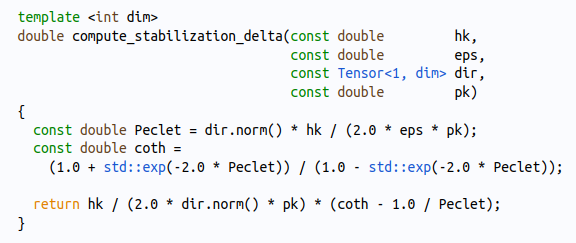
\includegraphics[width=8cm]{images/supg/step63}\\
{\captionfont Taken from step-63 webpage 
at \url{https://www.dealii.org/current/doxygen/deal.II/step_63.html}}
\end{center}

The expression above is also found at p. 617 in \textcite{lomw12}.
Note that Hughes \& Brooks \cite{hubr82} replace the costly 'coth' term by an asymptotic curve:

\begin{center}
\includegraphics[width=8cm]{images/supg/hubr82}\\
{\captionfont Taken from \cite{hubr82}. Here $\alpha$ is the Peclet number and the vertical axis
is the term $ \coth (\Penb) -1/\Penb$.}
\end{center}


\item
Codina (2000) (see Eq.39 of \cite{codi00}, see also Eq.2.64 of \textcite{dohu03}) defines $\tau$ as follows:
\[
\tau_2= \left( \frac{2 |\vec\upnu|}{h} + \frac{4 \kappa}{h^2} + \sigma   \right)^{-1}
\]
where $\sigma$ is a reaction term (which we neglect in what follows). This equation 
can be re-written:
\[
\tau_2= \frac{h}{2 |\vec\upnu|} \left( 1 + \frac{1}{\Penb} \right)^{-1}
\]



\item In \textcite{dohu03} we find the expression proposed by Shakib and co-workers (see Eq. 3.59 of \cite{shhj91}):
\[
\tau_3=\left( \left(\frac{2|\vec\upnu|}{h} \right)^2 
+9 \left(\frac{4\kappa}{h^2} \right)^2 + \sigma^2  \right)^{-1/2}
= \frac{h}{2|\vec\upnu|} \left(  1 + \frac{9}{\Penb^2} 
+ \left(\frac{h}{2|\vec\upnu|} \sigma  \right)^2 \right)^{-1/2}
\]

\item
Braun \cite{brau03} uses 
\[
\tau_4 = \frac{h}{|\vec\upnu| \sqrt{15}} = \frac{h}{2|\vec\upnu|} \frac{2}{\sqrt{15}} 
\]
This formula is independent of $\Penb$ and is also in \textcite{bogs04} (2004).
It is also used in Hughes \& Brooks (1982) \cite{hubr82} for pure advection problems in 1D
and this value is attributed to Raymond \& Garder (1976)  \cite{raga76}.

\item Following \textcite{teos00} (see also Appendix A of Thieulot (2011) \cite{thie11}):
\[
\tau_5 = \left( \frac{2 |\vec{\upnu}|}{h} + \frac{1}{\theta \delta t} + \frac{\kappa}{h^2} \right)^{-1}  
\]
Crank-Nicolson: $\theta=1/2$, CFL condition yields $\delta t = C \frac{h}{|\vec\upnu|}$ so 
\[
\tau_5 = \left( \frac{2 |\vec{\upnu}|}{h} + \frac{2}{\delta t}+  \frac{\kappa}{h^2}  \right)^{-1}  
= \left( \frac{2 |\vec{\upnu}|}{h} + \frac{2 v}{C h} +  \frac{\kappa}{h^2}  \right)^{-1}  
= \frac{h}{2 |\vec{\upnu}|}  \left( 1 + \frac{1}{C} + \frac{1}{4 \Penb} \right)^{-1} \nn 
\]
Note that the velocity in the CFL criterion is the maximum velocity in the domain, while 
in all other expressions above for $\tau_i$ it is the velocity in the cell/element. 
By doing so, the relationship  for $\tau_5$ is actually only valid for the cell with the 
highest velocity. 
Also, this has been used in the context of SUPG methods for the Navier-Stokes equations, 
not advection-diffusion equations! This approach is then not considered further.

\item \textcite{frhm04} (2004) use the following formula which originates from 
\textcite{frfh92} (1992): if $0\le \Penb < 1$ then
$\tau = \frac{h}{2 |\vec\upnu|} \Penb$ and if $\Penb \ge 1$ then $\tau = \frac{h}{2 |\vec\upnu|}$.
Note however that their definition of the Peclet number includes a scalar parameter $m$ which is 
the minimum between 1/3 and and 2$C_k$ where the calculation of this parameter is discussed in 
Remarks 4 and 5 of \cite{frfh92}. The authors conclude that for linear quadrilaterals the value
1/3 should be used while for biquadratic elements 1/12 should be preferred.
The same approach is found in \textcite{brbf92} (1992). 

\item Knobloch \cite{knob08} discusses other choices of $\tau$.


\end{enumerate}

Quoting Donea \& Huerta: "It is obvious that $\tau$ must vanish when the mesh is refined (no stabilisation
is necessary for a fine enough mesh)" and "Numerical experiments seem to indicate that for 
finite elements of order $p$ the value of the stabilisation parameter should be approximately 
$\tau/p$."

Let us define the dimensionless coefficient 
$\gamma_j=\frac{\tau_j}{h/2|\vec\upnu|}$ and 
plot this quantity against the Peclet number:

\begin{center}
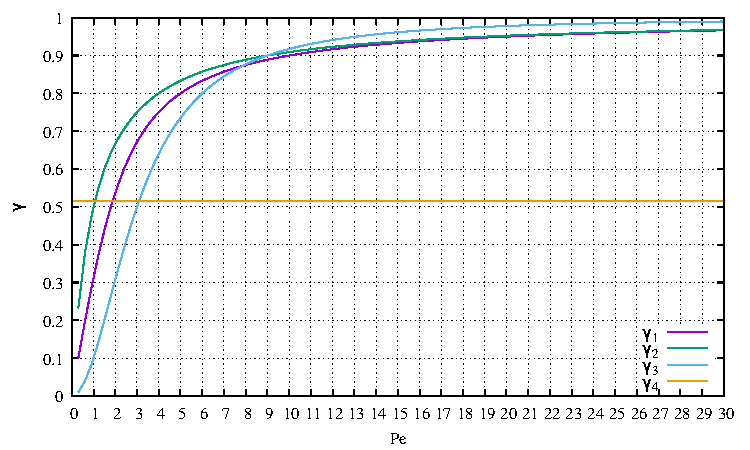
\includegraphics[width=10cm]{images/supg/gamma} 
\end{center}

In the case when the equation to be stabilised is a pure advection equation, 
then $\Penb\rightarrow \infty$ so 
\[
\gamma_1 \rightarrow 1/p  \quad
\gamma_2 \rightarrow 1 \quad
\gamma_3 \rightarrow 1 \quad
\gamma_4 \simeq 0.52 \quad
\gamma_5 \rightarrow (1+C^{-1})^{-1} 
\]
Note that in most versions above (except $\tau_1$) 
$\tau$ does not depend on the order $p$ of the basis functions.
Is it an omission?

Finally it is worth mentioning that \textcite{dohu03} argue that $\tau$ should 
ideally take different values at the corners and at the mid-side nodes for quadratic elements (p.~61).

%------------------------------
\subsection{Some remarks about Appendix A of Thieulot (2011) \cite{thie11}}
\label{ss:appAthie11}

In the \douar paper \cite{brtf08} or the \fantom paper \cite{thie11},
The advection matrix is simply modified and computed as follows:
\[
({\K}_a^e)_{SUPG}
=
\int_{x_k}^{x_{k+1}}   ({\vec \bN}^\star)^T \rho C_p \vec\upnu \cdot {\bm B} dx  
\quad\quad
{\text with}
\quad\quad
{\vec \bN}^\star= {\vec \bN} + \tau \vec \upnu \cdot {\bm B}
\]
Note that we can also write 
\[
({\K}_a^e)_{SUPG}
=
\int_{x_k}^{x_{k+1}}   {\vec \bN}^T \rho C_p \vec\upnu \cdot {\bm B} dx  
+
\int_{x_k}^{x_{k+1}}  \tau (\vec \upnu \cdot {\bm B})^T   \rho C_p (\vec\upnu \cdot {\bm B}) dx  
\]
and we see that the SUPG method introduces and additional term that is akin to 
a diffusion term in the direction of the flow.
This can be seen by looking at the advection matrix a regular grid of 1D 
elements of size $h$:
\[
({\K}_a^e)_{SUPG}=
{\K}_a^e
+
\rho C_p
\frac{\tau u^2}{h}
\left(
\begin{array}{cc}
1 & -1 \\ \\
-1 & 1
\end{array}
\right)
\]
The additional matrix has the same structure as the 1D diffusion matrix matrix in \ref{sec:diff1D}.

The parameter $\tau$ is chosen as follows \cite{teos00}:
\begin{equation}
\tau= \left(\frac{1}{\tau_1} + \frac{1}{\tau_2} + \frac{1}{\tau_3} \right)^{-1}
\qquad
\tau_1=\frac{h}{2 |\vec\upnu|},
\quad
\tau_2 = \theta \; \delta t,
\quad
\tau_3 = \frac{h^2 \rho C_p}{k}
\label{tausupg}
\end{equation}
where $h$ is a measure of the element size and $\theta$ is related to the time
discretisation scheme ($\theta$ = 1/2 corresponds to a mid-point implicit scheme),
and we can define $\gamma=\tau |\vec\upnu|/h$ (see Appendix A of \cite{thie11}). 

A typical test case for testing an advection scheme is the step advection benchmark 
(see for instance Donea \& Huerta (2003) \cite{dohu03}). At $t=0$, 
a field $T(x)$ is prescribed in a 1D domain of unit length. For $x\le 1/4$ we have $T(x)=1$ and 
$T(x)=0$ everywhere else as shown on the following figure:
\begin{center}
\includegraphics[width=8cm]{images/supg/fantom3}\\
{\captionfont Taken and modified from Thieulot (2011) \cite{thie11}}
\end{center}
The prescribed velocity is $\upnu=1$, 50 elements are used ($h=0.02$) and 250 time steps are 
carried out with $\delta t=0.1h/\upnu=0.002$ (CFL number of 0.1).
Then it follows that $\tau_3=\infty$ (no diffusion, i.e. $k=0$) and 
\[
\tau
= \left(\frac{2}{0.02} + \frac{2}{0.002} \right)^{-1}
= \left(\frac{1}{0.01} + \frac{1}{0.001} \right)^{-1}
= \left(\frac{1}{0.01} (1 + \frac{1}{10})  \right)^{-1}
= 0.01 \left(\frac{11}{10}  \right)^{-1}
\simeq 0.009091
\]
which yields $\gamma = 0.00909/0.02=0.4545...$
Using this value leads to a desired removal of the oscillations through a small
amount of numerical diffusion. Braun \cite{brau03} argues for a constant
$\gamma=1/\sqrt{15}=0.258$ (citing Hughes \& Brooks (1982) \cite{hubr82}), 
which effect is also shown in the figure above. This 
value is arguably too large and introduces an undesirable diffusion. Note that this same value is 
to be found in \textcite{bogs04} (2004). The authors then state that 
"for 1D pure advection problems, this choice maximizes the phase accuracy in the semidiscrete
equation" and cite Raymond \& Gardner (1976) \cite{raga76} as source. 

Another classic example of advection testing is a 2d problem where (for example) a cylinder, a Gaussian 
and a cone are prescribed and advected with a velocity field (see for instance \cite{dohu03}). 

\begin{center}
\includegraphics[width=0.45\textwidth]{images/supg/supg1}
\includegraphics[width=0.45\textwidth]{images/supg/supg2}\\
{\captionfont After a $2\pi$ rotation and in the absence of stabilisation we see that the temperature field
showcases clearly visible ripples.}
\end{center}

\begin{remark}
Note that \aspect{} originally did not rely on the SUPG formulation to stabilise the 
advection(-diffusion) equations\cite{krhb12}. It instead relied on the Entropy Viscosity
formulation \cite{gupp10,gupp11}.
It is only during the 6th Hackathon in May 2019 that the SUPG was introduced on the code.
Note that the \aspect{} implementation is based on the deal.II step 
63\footnote{\url{https://www.dealii.org/developer/doxygen/deal.II/step_63.html}}.
\end{remark}


%-----------------------------------------------------
\subsection{A note about linear elements - artificial diffusion}

We have seen in Section~\ref{ss:femvsfdm} that the discretised advection-diffusion equation 
in 1D can be written in a manner akin to the Finite Difference method:
\[
\frac{u}{2h}
\left[
\left(1-\frac{1}{\Penb}\right) T_{i+1} + \frac{2}{\Penb} T_i - \left(1+\frac{1}{\Penb}\right)T_{i-1} 
\right] = f
\]
and we show in \stone~65 that the solution is far from accurate for $\Penb>1$ (i.e. systems where advection 
dominates over diffusion). Let us ask ourselves the 
following question: could we come up with a modified version of the equation above which 
guarantees an exact solution on a uniform mesh of linear elements?

Essentially, we are looking for $A$, $B$ and $C$ such that 
{\color{red} not sure I understand this sentence} 
\[
A T_{i+1} + BT_i + C T_{i-1} = f
\]
One can show (see Donea \& Huerta \cite{dohu03}) that a successful 
candidate formulation is\footnote{where we have used $\coth(x)=(\exp(x)-\exp(-x))/(\exp(x)+\exp(-x))$}:
\[
\frac{u}{2h}
\left[
\left(1-\coth(\Penb) \right) T_{i+1} + 2 \coth(\Penb) T_i - \left(1+\coth(\Penb)\right) T_{i-1} 
\right] = f
\]
\todo[inline]{I need to better understand this!}
which can be arranged into the following form:
\begin{equation}
u
\frac{T_{i+1}-T_{i-1}}{2h_x}
-
(\kappa+ \tilde{\kappa})
\frac{T_{i-1}-2T_i+T_{i+1}}{h_x^2}
= \frac{f}{\rho_0 C_p}
\end{equation}
where 
$\tilde{\kappa}$ is known as artificial (numerical) diffusion (dissipation) given by
\[
\tilde{\kappa}=\beta \frac{u h}{2} = \beta \kappa \Penb
\qquad
\text{with}
\qquad
\beta = \coth (\Penb) - \frac{1}{\Penb}
\]
where $\Penb$ is the (dimensionless) Peclet number defined as: \index{general}{Peclet Number}
\[
\boxed{
\Penb= \frac{u h }{2 \kappa}
}
\]
If $\Penb>1$ we say the problem is advection-dominated, 
else if $\Penb<1$ we say the problem is diffusion-dominated.

The $\beta(\Penb)$ factor is shown in the following figure:
\begin{center}
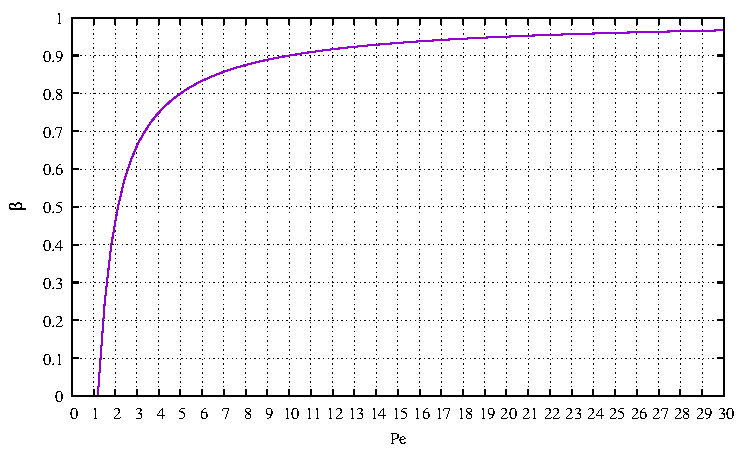
\includegraphics[width=10cm]{images/supg/beta}\\
{\captionfont Note that the value of $\beta$ is positive only for $\Penb>1$.}
\end{center}


One can also define $\tilde{k}=\rho_0 C_p \tilde{\kappa}$ so that 
the discretised 1D advection-diffusion becomes:
\begin{equation}
\rho_0 C_p u \frac{T_{i+1}-T_{i-1}}{2h_x}
- (k+ \tilde{k}) \frac{T_{i-1}-2T_i+T_{i+1}}{h_x^2}
= f 
\end{equation}
or, in its continuous formulation:
\begin{eqnarray}
\rho_0 C_p u \frac{dT}{dx} - (k+ \tilde{k}) \frac{d^2T}{dx^2} &=& f \nn\\
\rho_0 C_p u \frac{dT}{dx}
- \tilde{k} \frac{d^2T}{dx^2} 
- k \frac{d^2T}{dx^2} &=& f \nn\\
\rho_0 C_p u \frac{dT}{dx}
- \rho_0 C_p \beta \frac{u h}{2} \frac{d^2T}{dx^2} 
- k \frac{d^2T}{dx^2} &=& f
\end{eqnarray}





%-----------------------------------------------------
\subsection{A note about linear elements - bubble functions \& Petrov-Galerkin formulation}

Let us assume that $u>0$, i.e. advection goes from left to right. 
Node $i-1$ is said to be on the upstream side of node $i$, and node $i+1$
is on the downstream side of node . In Petrov FEM, instead of selecting the weight functions to be the
same as the standard basis functions, we distort them as shown below.

\index{general}{Bubble Function}
The distortion is based on so-called bubble functions since they have zero
values on the nodes and they are nonzero on elements' interiors.
For instance one can take
\begin{eqnarray}
{\bN}^\star_1(r)&=&\frac{1}{2}(1-r)-\frac{3}{4}\beta(1-r^2) \\
{\bN}^\star_2(r)&=&\frac{1}{2}(1+r)+\frac{3}{4}\beta(1-r^2) 
\end{eqnarray}
as test/weight functions
where $\beta$ is a parameter that controls the amount of upwinding. 

The elemental advection matrix is then given by:
\begin{center}
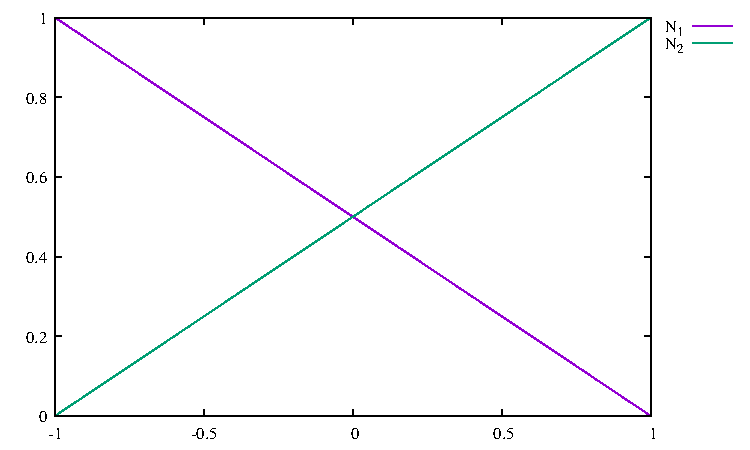
\includegraphics[width=6cm]{images/supg/bubble1}
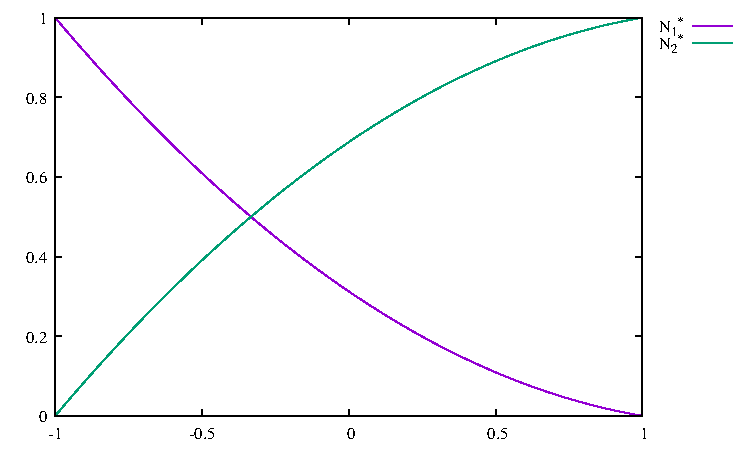
\includegraphics[width=6cm]{images/supg/bubble2}\\
{\captionfont Left: standard $Q_1$ test functions; Right: modified ($Q_1$+bubble) functions
for $\beta=0.25$}
\end{center}

\[
r = 2(x-x_k)/(x_{k+1}-x_{k}) -1 =2(x-x_k)/h  -1
\]
then 
\[
dr = \frac{2}{h} dx
\]
or
\[
dx=\frac{h}{2} dr
\]


\begin{eqnarray}
{\K}_a^e 
&=& \int_{x_k}^{x_{k+1}}   ({\vec \bN}^\star)^T \rho C_p \vec\upnu \cdot {\bm B} \; dx  \nn\\
&=& \frac{h}{2} \int_{-1}^{+1}   ({\vec \bN}^\star)^T \rho C_p \vec\upnu \cdot {\bm B} \; dr  \nn\\
&=& \frac{h}{2} \int_{-1}^{+1} 
\left(\begin{array}{c}
{\bN}_1^\star \\ {\bN}_2^\star 
\end{array}\right)
\rho C_p u \left( \frac{d\bN_1}{dr} \; \frac{d\bN_2}{dr} \right)  dr \nn\\
&=& 
\frac{h}{2} \rho C_p u \int_{-1}^{+1} 
\left(\begin{array}{c}
{\bN}_1 \\ {\bN}_2
\end{array}\right)
\left( \frac{d\bN_1}{dr} \; \frac{d\bN_2}{dr} \right)  dr
+
\frac{h}{2} \rho C_p u \int_{-1}^{+1} 
\left(\begin{array}{c}
-\frac{3}{4}\beta(1-r^2) \\ +\frac{3}{4}\beta(1-r^2) 
\end{array}\right)
\left( \frac{d\bN_1}{dr} \; \frac{d\bN_2}{dr} \right)  dr 
\nn\\
&=& 
\frac{h}{2} \rho C_p u \int_{-1}^{+1} 
\left(\begin{array}{c}
\frac12 (1-r) \\ \frac12(1+r)
\end{array}\right)
\left( -\frac12 \; \frac12 \right)  dr
+
\frac{h}{2} \rho C_p u \int_{-1}^{+1} 
\left(\begin{array}{c}
-\frac{3}{4}\beta(1-r^2) \\ +\frac{3}{4}\beta(1-r^2) 
\end{array}\right)
\left( -\frac12 \; \frac12 \right)  dr  
\nn\\
&=& \rho C_p u \frac{h}{8}\int_{-1}^{+1} 
\left(\begin{array}{cc}
-(1-r) & (1-r)  \\
-(1+r) & (1+r)
\end{array}\right)  dr
+
\frac{3h}{16}\beta
\rho C_p u \int_{-1}^{+1} 
\left(\begin{array}{cc}
(1-r^2) & -(1-r^2) \\
-(1-r^2) & (1-r^2) 
\end{array}\right)  dr
\nn\\
&=& \rho C_p u \frac{h}{8}
\left(\begin{array}{cc}
-2 & 2 \\
-2 & 2
\end{array}\right)  
+
\frac{3h}{16}\beta
\rho C_p u 
\left(\begin{array}{cc}
4/3 & -4/3 \\
-4/3 & 4/3 
\end{array}\right)   \nn\\
&=& \rho C_p u \frac{h}{4}
\left(\begin{array}{cc}
-1 & 1 \\
-1 & 1
\end{array}\right) 
+
\frac{h}{4}\beta
\rho C_p u 
\left(\begin{array}{cc}
1 & -1 \\
-1 & 1 
\end{array}\right)  
\end{eqnarray}
We see that this additional matrix is akin to ${\K}_d^e$ (albeit with a 
different diffusion coefficient).

 %-----------
\newpage %-----------------------------------------------------------------------------------------
\section{Assigning values to quadrature points \label{ss:averagings}} \input{averagings} %------
\newpage %-----------------------------------------------------------------------------------------
\section{Matrix (Sparse) storage} \begin{flushright} {\tiny {\color{gray} storage.tex}} \end{flushright}
%~~~~~~~~~~~~~~~~~~~~~~~~~~~~~~~~~~~~~~~~~~~~~~~~~~~~~~~~~~~~~~~~~~~~~~~~~~~~~~~~~~~~~~~~~~~~~~~~~~

The FE matrix (or the blocks which compose it) 
is the result of the assembly process of all elemental matrices. 
Its size can become quite large when the resolution is being increased (from thousands
of lines/columns to tens of millions).

One important property of the matrix is its sparsity. Typically mush less than 1\% of the 
matrix terms is not zero and this means that the matrix storage can and {\it should} be optimised. 
Clever storage formats were designed early on since the amount of RAM memory in computers
was the limiting factor 3 or 4 decades ago \cite{saad}.

There are several standard formats, e.g.:
\begin{itemize}
\item compressed sparse row format (CSR) \index{general}{CSR} \index{general}{Compressed Sparse Row}
\item compressed sparse column format (CSC) \index{general}{CSC} \index{general}{Compressed Sparse Column}
\item the Coordinate Format (COO)
\item Skyline Storage Format
\end{itemize}

I focus on  the CSR format in what follows since it is the most common format 
and it is the one used in \elefant. 

%..............................................................................
\subsection{2D domain - $Q_1$ - One degree of freedom per node}

Let us consider again the  $3\times2$ element grid which counts 12 nodes.

\begin{center}
\begin{flushright} {\tiny {\color{gray} (tikz\_3x2.tex)}} \end{flushright}
%~~~~~~~~~~~~~~~~~~~~~~~~~~~~~~~~~~~~~~~~~~~~~~~~~~~~~~~~~~~~~~~~~~~~~~~~~~~~~~~~~~~~~~~~~~~~~~~~~~

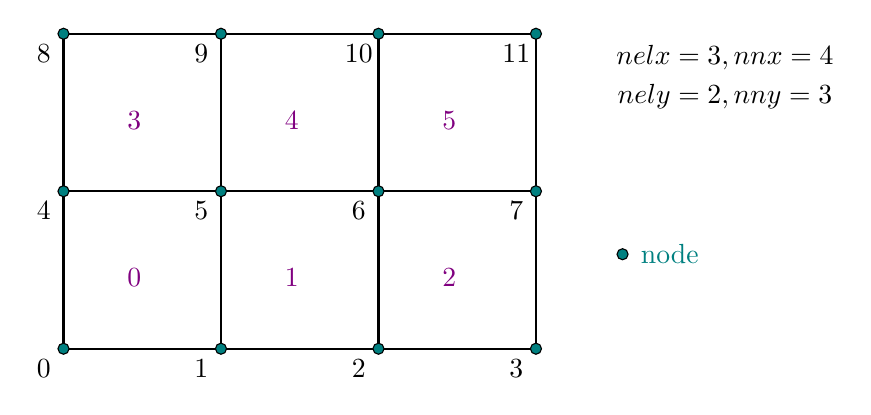
\begin{tikzpicture}
%\draw[step=0.5cm,gray,very thin] (0,0) grid (9,5); %background grid

\draw[thick] (1,1) -- (7,1) -- (7,5) -- (1,5) -- cycle;  
\draw[thick] (1,3) -- (7,3) ;
\draw[thick] (3,1) -- (3,5) ;
\draw[thick] (5,1) -- (5,5) ;

\draw[black,fill=teal] (1,1)     circle (2pt); 
\draw[black,fill=teal] (3,1)     circle (2pt); 
\draw[black,fill=teal] (5,1)     circle (2pt); 
\draw[black,fill=teal] (7,1)     circle (2pt); 

\draw[black,fill=teal] (1,3)     circle (2pt); 
\draw[black,fill=teal] (3,3)     circle (2pt); 
\draw[black,fill=teal] (5,3)     circle (2pt); 
\draw[black,fill=teal] (7,3)     circle (2pt); 

\draw[black,fill=teal] (1,5)     circle (2pt); 
\draw[black,fill=teal] (3,5)     circle (2pt); 
\draw[black,fill=teal] (5,5)     circle (2pt); 
\draw[black,fill=teal] (7,5)     circle (2pt); 

\node[] at (0.75,0.75) {0};
\node[] at (2.75,0.75) {1};
\node[] at (4.75,0.75) {2};
\node[] at (6.75,0.75) {3};

\node[] at (0.75,2.75) {4};
\node[] at (2.75,2.75) {5};
\node[] at (4.75,2.75) {6};
\node[] at (6.75,2.75) {7};

\node[] at (0.75,4.75) {8};
\node[] at (2.75,4.75) {9};
\node[] at (4.75,4.75) {10};
\node[] at (6.75,4.75) {11};

\node[violet] at (1.9,1.9) {0};
\node[violet] at (3.9,1.9) {1};
\node[violet] at (5.9,1.9) {2};
\node[violet] at (1.9,3.9) {3};
\node[violet] at (3.9,3.9) {4};
\node[violet] at (5.9,3.9) {5};

\draw[black,fill=teal] (8.1,2.2) circle (2pt); 
\node[] at (8.7,2.2) {{\color{teal}node}};

\node[] at (9.4,4.7) {$nelx=3, nnx=4$};
\node[] at (9.4,4.2) {$nely=2, nny=3$};

\end{tikzpicture}

\end{center}

\noindent In the case there is only a single degree of freedom per node, the 
assembled FEM matrix ${\bm M}$ will look like this:
\[
{\bm M}=
\left(
\begin{array}{cccccccccccc}
\Box & \Box &      &      & \Box & \Box &      &      &      &      &      &      \\
\Box & \Box & \Box &      & \Box & \Box & \Box &      &      &      &      &      \\
     & \Box & \Box & \Box &      & \Box & \Box & \Box &      &      &      &      \\
     &      & \Box & \Box &      &      & \Box & \Box &      &      &      &      \\
\Box & \Box &      &      & \Box & \Box &      &      & \Box & \Box &      &      \\
\Box & \Box & \Box &      & \Box & \Box & \Box &      & \Box & \Box & \Box &      \\
     & \Box & \Box & \Box &      & \Box & \Box & \Box &      & \Box & \Box & \Box \\
     &      & \Box & \Box &      &      & \Box & \Box &      &      & \Box & \Box \\
     &      &      &      & \Box & \Box &      &      & \Box & \Box &      &      \\
     &      &      &      & \Box & \Box & \Box &      & \Box & \Box & \Box &      \\
     &      &      &      &      & \Box & \Box & \Box &      & \Box & \Box & \Box \\
     &      &      &      &      &      & \Box & \Box &      &      & \Box & \Box 
\end{array}
\right)
\]
where the $\Box$ stand for non-zero terms.
This matrix structure stems from the fact that
\begin{itemize}
\item node 0 sees nodes 0,1,4,5 (1st line/column of the matrix)
\item node 1 sees nodes 0,1,2,4,5,6 (2nd line/column of the matrix)
\item node 2 sees nodes 1,2,3,5,6,7 (3rd line/column of the matrix)
\item node 3 sees nodes 2,3,6,7
\item node 4 sees nodes 0,1,4,5,8,9
\item node 5 sees nodes 0,1,2,4,5,6,8,9,10 
\item node 6 sees nodes 1,2,3,5,6,7,9,10,11
\item node 7 sees nodes 2,3,6,7,10,11
\item node 8 sees nodes 4,5,8,9
\item node 9 sees nodes 4,5,6,8,9,10
\item node 10 sees nodes 5,6,7,9,10,11 
\item node 11 sees nodes 6,7,10,11 (last line/column of the matrix)
\end{itemize}
In light thereof, we have
\begin{itemize}
\item 4 corner nodes which have 4 neighbours (counting themselves) 
\item 2(nnx-2) nodes which have 6 neighbours
\item 2(nny-2) nodes which have 6 neighbours
\item (nnx-2)$\times$(nny-2) nodes which have 9 neighbours
\end{itemize}
In total, the number of non-zero terms in the matrix above is then:
\[
NZ=4\times4+4\times6+2\times6+2\times9=70
\]
and in general, we would then have:
\[
NZ=4\times4+[2(nnx-2)+2(nny-2)]\times6 + (nnx-2)(nny-2)\times9
\]
Let us temporarily assume $nnx=nny=n$. The matrix size (total
number of unknowns) is then $N=n^2$ and  
\[
NZ=16+24(n-2)+9(n-2)^2
\]
A full matrix array would contain $N^2=n^4$ terms. 
The ratio of $NZ$ (the actual number of reals to store)
to the full matrix size (the number of reals a full matrix contains) is then 
\[
R = \frac{16+24(n-2)+9(n-2)^2}{n^4}
\]
It is then obvious that when $n$ is large enough $R \sim 1/n^2$.

CSR stores the nonzeros of the matrix row by row, in a
single indexed array A of double precision  numbers.
Another array COLIND contains the column index of each
corresponding entry in the A array. A third integer array RWPTR
contains pointers to the beginning of each row, which an additional pointer to
the first index following the nonzeros of the matrix A.
A and COLIND have length NZ and RWPTR has length N+1.

In the case of the here-above matrix, the arrays COLIND and RWPTR will look like:
\begin{eqnarray}
COLIND&=&(0,1,4,5, \; 0,1,2,4,5,6, \; 1,2,3,5,6,7, ..., 6,7,10,11) \nn\\
RWPTR &=&(0,4,10,16, ... )   \nn
\end{eqnarray}


%..............................................................................
\subsection{2D domain - $Q_1$ - Symmetric matrix CSR storage} \label{ss:symmcsrss}

If the matrix is symmetric, i.e. ${\bm M}={\bm M}^T$, then we may wish to 
only store half of it, always in the interest of saving memory. 
Only the following remaining $\Box$ entries are relevant now:
\[
{\bm M}=
\left(
\begin{array}{cccccccccccc}
\Box & \Box &      &      & \Box & \Box &      &      &      &      &      &      \\
     & \Box & \Box &      & \Box & \Box & \Box &      &      &      &      &      \\
     &      & \Box & \Box &      & \Box & \Box & \Box &      &      &      &      \\
     &      &      & \Box &      &      & \Box & \Box &      &      &      &      \\
     &      &      &      & \Box & \Box &      &      & \Box & \Box &      &      \\
     &      &      &      &      & \Box & \Box &      & \Box & \Box & \Box &      \\
     &      &      &      &      &      & \Box & \Box &      & \Box & \Box & \Box \\
     &      &      &      &      &      &      & \Box &      &      & \Box & \Box \\
     &      &      &      &      &      &      &      & \Box & \Box &      &      \\
     &      &      &      &      &      &      &      &      & \Box & \Box &      \\
     &      &      &      &      &      &      &      &      &      & \Box & \Box \\
     &      &      &      &      &      &      &      &      &      &      & \Box 
\end{array}
\right)
\]
We see that the number of nonzeros is now 
\[
NZ_{symm}= \frac{NZ-n}{2}+n
\]
and in this case $NZ_{symm}=(70-12)/2+12=41$.
Then 
\begin{eqnarray}
COLIND&=&(0,1,4,5, \; 1,2,4,5,6, \; 3,5,6,7, ..., ,11) \nn\\
RWPTR &=&(0,4,9,14, ... )   \nn
\end{eqnarray}

In case the numbering is Fortran-like, then 
\begin{eqnarray}
ja=COLIND&=&(
1, 2, 5, 6, \quad  2, 3, 5, 6, 7, \quad 3, 4, 6, 7, 8, \quad      
4, 7, 8, \quad  5, 6, 9, 10, \quad 6, 7, 9, 10, 11, \nn\\
&& 7, 8, 10, 11, 12, \quad 8, 11, 12, \quad 9, 10, \quad 10, 11, \quad  11, 12, \quad 12) \nn\\
ia=RWPTR &=&(1, 5, 10, 15, 18, 22, 27, 32, 35, 37, 39, 41, 42)  \nn
\end{eqnarray}

%..............................................................................
\subsection{2D domain - $Q_1$ - Two degrees of freedom per node}

When there are now two degrees of freedom per node, such as in the case 
of the Stokes equation in two-dimensions, the size of the $\K$ matrix 
is given $NfemV=nnx*nny*ndofV$ where $NfemV$ is the total number of 
velocity degrees of freedom.

\begin{center}
\input{tikz/tikz_3x2_two}
\end{center}

In the case of the small grid above, we have then $NfemV=24$ and
elemental matrices are now $8\times8$ in size.

We still have
\begin{itemize}
\item $4$ corner nodes which have 4 neighbours
\item $2(nnx-2)$ nodes which have 6 neighbours
\item $2(nny-2)$ nodes which have 6 neighbours
\item $(nnx-2)\cdot(nny-2)$ nodes which have 9 neighbours,
\end{itemize}
but now each degree of freedom from a node sees the other two
degrees of freedom of another node too.
In that case, the number of nonzeros has been multiplied by four
and the assembled FEM matrix looks like:
\begin{equation}
\left(
\begin{array}{cccccccccccccccccccccccc}
\Box&\Box & \Box&\Box &  &  &  &  & \Box&\Box & \Box&\Box &  &  &  &  &  &  &  &  &  &  &  &  \\
\Box&\Box & \Box&\Box &  &  &  &  & \Box&\Box & \Box&\Box &  &  &  &  &  &  &  &  &  &  &  &  \\
\Box&\Box & \Box&\Box & \Box&\Box &  &  & \Box&\Box & \Box&\Box & \Box&\Box &  &  &  &  &  &  &  &  &  &  \\
\Box&\Box & \Box&\Box & \Box&\Box &  &  & \Box&\Box & \Box&\Box & \Box&\Box &  &  &  &  &  &  &  &  &  &  \\
 &  & \Box&\Box & \Box&\Box & \Box&\Box &  &  & \Box&\Box & \Box&\Box & \Box&\Box &  &  &  &  &  &  &  &  \\
 &  & \Box&\Box & \Box&\Box & \Box&\Box &  &  & \Box&\Box & \Box&\Box & \Box&\Box &  &  &  &  &  &  &  &  \\
 &  &  &  & \Box&\Box & \Box&\Box &  &  &  &  & \Box&\Box & \Box&\Box &  &  &  &  &  &  &  &  \\
 &  &  &  & \Box&\Box & \Box&\Box &  &  &  &  & \Box&\Box & \Box&\Box &  &  &  &  &  &  &  &  \\
\Box&\Box & \Box&\Box &  &  &  &  & \Box&\Box & \Box&\Box &  &  &  &  & \Box&\Box & \Box&\Box &  &  &  &  \\
\Box&\Box & \Box&\Box &  &  &  &  & \Box&\Box & \Box&\Box &  &  &  &  & \Box&\Box & \Box&\Box &  &  &  &  \\
\Box&\Box & \Box&\Box & \Box&\Box &  &  & \Box&\Box & \Box&\Box & \Box&\Box &  &  & \Box&\Box & \Box&\Box & \Box&\Box &  &  \\
\Box&\Box & \Box&\Box & \Box&\Box &  &  & \Box&\Box & \Box&\Box & \Box&\Box &  &  & \Box&\Box & \Box&\Box & \Box&\Box &  &  \\
 &  & \Box&\Box & \Box&\Box & \Box&\Box &  &  & \Box&\Box & \Box&\Box & \Box&\Box &  &  & \Box&\Box & \Box&\Box & \Box&\Box \\
 &  & \Box&\Box & \Box&\Box & \Box&\Box &  &  & \Box&\Box & \Box&\Box & \Box&\Box &  &  & \Box&\Box & \Box&\Box & \Box&\Box \\
 &  &  &  & \Box&\Box & \Box&\Box &  &  &  &  & \Box&\Box & \Box&\Box &  &  &  &  & \Box&\Box & \Box&\Box \\
 &  &  &  & \Box&\Box & \Box&\Box &  &  &  &  & \Box&\Box & \Box&\Box &  &  &  &  & \Box&\Box & \Box&\Box \\
 &  &  &  &  &  &  &  & \Box&\Box & \Box&\Box &  &  &  &  & \Box&\Box & \Box&\Box &  &  &  &  \\
 &  &  &  &  &  &  &  & \Box&\Box & \Box&\Box &  &  &  &  & \Box&\Box & \Box&\Box &  &  &  &  \\
 &  &  &  &  &  &  &  & \Box&\Box & \Box&\Box & \Box&\Box &  &  & \Box&\Box & \Box&\Box & \Box&\Box &  &  \\
 &  &  &  &  &  &  &  & \Box&\Box & \Box&\Box & \Box&\Box &  &  & \Box&\Box & \Box&\Box & \Box&\Box &  &  \\
 &  &  &  &  &  &  &  &  &  & \Box&\Box & \Box&\Box & \Box&\Box &  &  & \Box&\Box & \Box&\Box & \Box&\Box \\
 &  &  &  &  &  &  &  &  &  & \Box&\Box & \Box&\Box & \Box&\Box &  &  & \Box&\Box & \Box&\Box & \Box&\Box \\
 &  &  &  &  &  &  &  &  &  &  &  & \Box&\Box & \Box&\Box &  &  &  &  & \Box&\Box & \Box&\Box \\
 &  &  &  &  &  &  &  &  &  &  &  & \Box&\Box & \Box&\Box &  &  &  &  & \Box&\Box & \Box&\Box 
\end{array}
\right)\nonumber
\end{equation}
Note that the degrees of freedom are organised as follows: 
\[
(u_0,v_0,u_1,v_1,u_2,v_2, ... u_{11},v_{11})
\]
In general, we would then have:
\[
NZ=4 \left[4\times4+[2(nnx-2)+2(nny-2)]\times6 + (nnx-2)(nny-2)\times9 \right]
\]
and in the case of the small grid,
the number of non-zero terms in the matrix is then:
\[
NZ=4\left[4\times4+4\times6+2\times6+2\times9\right]=280
\]
In the case of the here-above matrix, the arrays COLIND and RWPTR will look like:
\begin{eqnarray}
COLIND&=&(0,1,2,3,8,9,10,11, \; 0,1,2,3,8,9,10,11,\; ...) \nn\\
RWPTR &=&(0,8,16,28, ... ) \nn
\end{eqnarray}

Assuming we are using $Q_1\times P_0$ elements, the structure of the matrix $\G_{el}^T$ is as follows
(the 6 pressure dofs are connected to 24 velocity dofs):

\begin{scriptsize}
\begin{equation}
\left(
\begin{array}{ccccccccccccccccccccccccc}
&0 & 1 & 2 & 3 & 4 & 5 & 6 & 7 & 8 & 9 & 10 & 11 & 12 & 13 & 14 & 15 & 16 & 17 & 18 & 19 & 20 & 21 & 22 & 23     \\
\Box&\Box & \Box&\Box &  &  &  &  & \Box&\Box & \Box&\Box &  &  &  &  &  &  &  &  &  &  &  &  \\
    &     & \Box&\Box & \Box&\Box &  &  &  &  & \Box&\Box & \Box&\Box &  &  &  &  &  &  &  &  &  &  \\
 & &     &     & \Box&\Box & \Box&\Box &  &  &  &  & \Box&\Box & \Box&\Box &  &  &  &  &  &  &  &    \\
 & & & &  & &     &     & \Box&\Box & \Box&\Box &  &  &  &  & \Box&\Box & \Box&\Box &  &  &  &      \\
 & & & & & &  & &     &     & \Box&\Box & \Box&\Box &  &  &  &  & \Box&\Box & \Box&\Box &  &       \\
 & &  & & & & & &  & &     &     & \Box&\Box & \Box&\Box &  &  &  &  & \Box&\Box & \Box&\Box        
\end{array}
\right)
\end{equation} 
\end{scriptsize}

\begin{center}
\input{tikz/csrStokes_3x2_ELEFANT}
\input{tikz/csrStokes_4x3_ELEFANT}
\input{tikz/csrStokes_5x4_ELEFANT}\\
{\captionfont From left to right: Nonzero structures of the assembled Stokes matrix for a 
$3\times 2$, $4\times 3$ and $5\times 4$ mesh of $Q_1\times P_0$ elements.}
\end{center}


Assuming we are now using $Q_1\times Q_1$ elements (without bubble), 
the structure of the matrix $\G_{el}^T$ is different: we now have 12 pressure dofs 
which are coupled to 24 velocity dofs:
\begin{scriptsize}
\begin{equation}
\left(
\begin{array}{ccccccccccccccccccccccccc}
 & 1 & 2 & 3 & 4 & 5 & 6 & 7 & 8 & 9 & 10 & 11 & 12 & 13 & 14 & 15 & 16 & 17 & 18 & 19 & 20 & 21 & 22 & 23 & 24    \\
0 &\Box&\Box & \Box&\Box &  &  &  &  & \Box&\Box & \Box&\Box &  &  &  &  &  &  &  &  &  &  &  &  \\
1 & \Box&\Box & \Box&\Box & \Box  & \Box  &  &  & \Box&\Box & \Box&\Box & \Box  & \Box  &  &  &  &  &  &  &  &  &  & \\
2 &  & & \Box&\Box & \Box  & \Box  & \Box  & \Box  & & & \Box&\Box & \Box  & \Box  & \Box  &\Box  &  &  &  &  &  &  &  & \\ 
3 &  & & &  & \Box  & \Box  & \Box  & \Box  & & & & & \Box  & \Box  & \Box  &\Box  &  &  &  &  &  &  &  & \\ 
\\
... \\
\\
9 & & & & & & & & &\Box &\Box &\Box &\Box & \Box  & \Box &  &  & & &\Box &\Box & \Box &\Box & &  \\
10 & & & & & & & & & & &\Box &\Box & \Box  & \Box & \Box & \Box & & &\Box &\Box & \Box &\Box &\Box & \Box \\
11 & & & & & & & & & & & & & \Box  & \Box & \Box & \Box & & & & & \Box &\Box &\Box & \Box \\
\end{array}
\right)
\end{equation} 
\end{scriptsize}

%..............................................................................
\subsection{2D domain - $Q_2$ - Two degrees of freedom per node}


When there are now two degrees of freedom per node, such as in the case 
of the Stokes equation in two-dimensions, the size of the $\K$ matrix 
is given $NfemV=nnx*nny*ndofV$ where $NfemV$ is the total number of 
velocity degrees of freedom. What is different here is that for $Q_2$
elements we have $nnx=2*nelx+1$ and $nny=2*nely+1$.

\begin{center}
\begin{flushright} {\tiny {\color{gray} (tikz\_3x2\_two\_Q2.tex)}} \end{flushright}
%~~~~~~~~~~~~~~~~~~~~~~~~~~~~~~~~~~~~~~~~~~~~~~~~~~~~~~~~~~~~~~~~~~~~~~~~~~~~~~~~~~~~~~~~~~~~~~~~~~

\begin{tikzpicture}
%\draw[step=0.5cm,gray,very thin] (0,0) grid (8,6); %background grid

\draw[thick] (1,1) -- (7,1) -- (7,5) -- (1,5) -- cycle;  
\draw[thick] (1,3) -- (7,3) ;
\draw[thick] (3,1) -- (3,5) ;
\draw[thick] (5,1) -- (5,5) ;

\draw[black,fill=teal] (1,1)     circle (2pt); 
\draw[black,fill=teal] (2,1)     circle (2pt); 
\draw[black,fill=teal] (3,1)     circle (2pt); 
\draw[black,fill=teal] (4,1)     circle (2pt); 
\draw[black,fill=teal] (5,1)     circle (2pt); 
\draw[black,fill=teal] (6,1)     circle (2pt); 
\draw[black,fill=teal] (7,1)     circle (2pt); 

\draw[black,fill=teal] (1,2)     circle (2pt); 
\draw[black,fill=teal] (2,2)     circle (2pt); 
\draw[black,fill=teal] (3,2)     circle (2pt); 
\draw[black,fill=teal] (4,2)     circle (2pt); 
\draw[black,fill=teal] (5,2)     circle (2pt); 
\draw[black,fill=teal] (6,2)     circle (2pt); 
\draw[black,fill=teal] (7,2)     circle (2pt); 

\draw[black,fill=teal] (1,3)     circle (2pt); 
\draw[black,fill=teal] (2,3)     circle (2pt); 
\draw[black,fill=teal] (3,3)     circle (2pt); 
\draw[black,fill=teal] (4,3)     circle (2pt); 
\draw[black,fill=teal] (5,3)     circle (2pt); 
\draw[black,fill=teal] (6,3)     circle (2pt); 
\draw[black,fill=teal] (7,3)     circle (2pt); 

\draw[black,fill=teal] (1,4)     circle (2pt); 
\draw[black,fill=teal] (2,4)     circle (2pt); 
\draw[black,fill=teal] (3,4)     circle (2pt); 
\draw[black,fill=teal] (4,4)     circle (2pt); 
\draw[black,fill=teal] (5,4)     circle (2pt); 
\draw[black,fill=teal] (6,4)     circle (2pt); 
\draw[black,fill=teal] (7,4)     circle (2pt); 

\draw[black,fill=teal] (1,5)     circle (2pt); 
\draw[black,fill=teal] (2,5)     circle (2pt); 
\draw[black,fill=teal] (3,5)     circle (2pt); 
\draw[black,fill=teal] (4,5)     circle (2pt); 
\draw[black,fill=teal] (5,5)     circle (2pt); 
\draw[black,fill=teal] (6,5)     circle (2pt); 
\draw[black,fill=teal] (7,5)     circle (2pt); 

\node[] at (0.85,0.7) {\tiny 0,1};
\node[] at (1.85,0.7) {\tiny 2,3};
\node[] at (2.85,0.7) {\tiny 4,5};
\node[] at (3.85,0.7) {\tiny 6,7};
\node[] at (4.85,0.7) {\tiny 8,9};
\node[] at (5.85,0.7) {\tiny 10,11};
\node[] at (6.85,0.7) {\tiny 12,13};

\node[] at (0.85,1.7) {\tiny 14,15};
\node[] at (1.85,1.7) {\tiny 16,17};
\node[] at (2.85,1.7) {\tiny 18,19};
\node[] at (3.85,1.7) {\tiny 20,21};
\node[] at (4.85,1.7) {\tiny 22,23};
\node[] at (5.85,1.7) {\tiny 24,25};
\node[] at (6.85,1.7) {\tiny 26,27};

\node[] at (0.85,2.7) {\tiny 28,29}; 
\node[] at (1.85,2.7) {\tiny 30,31}; 
\node[] at (2.85,2.7) {\tiny 32,33}; 
\node[] at (3.85,2.7) {\tiny 34,35}; 
\node[] at (4.85,2.7) {\tiny 36,37}; 
\node[] at (5.85,2.7) {\tiny 38,39}; 
\node[] at (6.85,2.7) {\tiny 40,41}; 

\node[] at (0.85,3.7) {\tiny 42,43}; 
\node[] at (1.85,3.7) {\tiny 44,45}; 
\node[] at (2.85,3.7) {\tiny 46,47}; 
\node[] at (3.85,3.7) {\tiny 48,49}; 
\node[] at (4.85,3.7) {\tiny 50,51}; 
\node[] at (5.85,3.7) {\tiny 52,53}; 
\node[] at (6.85,3.7) {\tiny 54,55}; 

\node[] at (0.85,4.7) {\tiny 56,57}; 
\node[] at (1.85,4.7) {\tiny 58,59}; 
\node[] at (2.85,4.7) {\tiny 60,61}; 
\node[] at (3.85,4.7) {\tiny 62,63}; 
\node[] at (4.85,4.7) {\tiny 64,65}; 
\node[] at (5.85,4.7) {\tiny 66,67}; 
\node[] at (6.85,4.7) {\tiny 68,69}; 

\node[violet] at (1.29,1.29) {0};
\node[violet] at (3.29,1.29) {1};
\node[violet] at (5.29,1.29) {2};
\node[violet] at (1.29,3.29) {4};
\node[violet] at (3.29,3.29) {5};
\node[violet] at (5.29,3.29) {6};

\draw[black,fill=teal] (8.1,2.2) circle (2pt); 
\node[] at (8.4,2.2) {$\vec\upnu$};

\end{tikzpicture}


\end{center}

In the case of the small grid above, we have then 
$nelx=3$, $nely=2$, so that $nnx=7$ and $nny=5$, and then
$NfemV=7*5*2=70$ and elemental matrices are now $18\times18$ in size.


\begin{center}
\begin{flushright} {\tiny {\color{gray} (tikz\_3x2\_Q2.tex)}} \end{flushright}
%~~~~~~~~~~~~~~~~~~~~~~~~~~~~~~~~~~~~~~~~~~~~~~~~~~~~~~~~~~~~~~~~~~~~~~~~~~~~~~~~~~~~~~~~~~~~~~~~~~

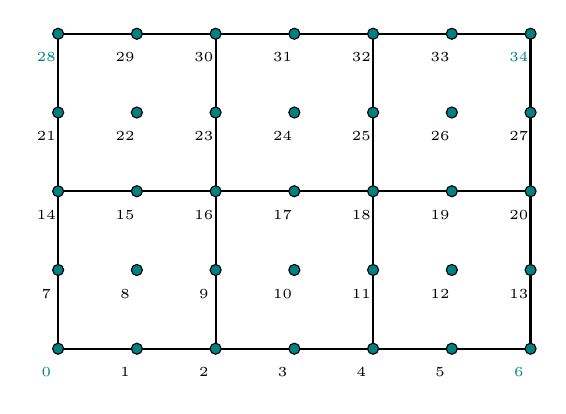
\begin{tikzpicture}
%\draw[step=0.5cm,gray,very thin] (0,0) grid (8,6); %background grid

\draw[thick] (1,1) -- (7,1) -- (7,5) -- (1,5) -- cycle;  
\draw[thick] (1,3) -- (7,3) ;
\draw[thick] (3,1) -- (3,5) ;
\draw[thick] (5,1) -- (5,5) ;

\draw[black,fill=teal] (1,1)     circle (2pt); 
\draw[black,fill=teal] (2,1)     circle (2pt); 
\draw[black,fill=teal] (3,1)     circle (2pt); 
\draw[black,fill=teal] (4,1)     circle (2pt); 
\draw[black,fill=teal] (5,1)     circle (2pt); 
\draw[black,fill=teal] (6,1)     circle (2pt); 
\draw[black,fill=teal] (7,1)     circle (2pt); 

\draw[black,fill=teal] (1,2)     circle (2pt); 
\draw[black,fill=teal] (2,2)     circle (2pt); 
\draw[black,fill=teal] (3,2)     circle (2pt); 
\draw[black,fill=teal] (4,2)     circle (2pt); 
\draw[black,fill=teal] (5,2)     circle (2pt); 
\draw[black,fill=teal] (6,2)     circle (2pt); 
\draw[black,fill=teal] (7,2)     circle (2pt); 

\draw[black,fill=teal] (1,3)     circle (2pt); 
\draw[black,fill=teal] (2,3)     circle (2pt); 
\draw[black,fill=teal] (3,3)     circle (2pt); 
\draw[black,fill=teal] (4,3)     circle (2pt); 
\draw[black,fill=teal] (5,3)     circle (2pt); 
\draw[black,fill=teal] (6,3)     circle (2pt); 
\draw[black,fill=teal] (7,3)     circle (2pt); 

\draw[black,fill=teal] (1,4)     circle (2pt); 
\draw[black,fill=teal] (2,4)     circle (2pt); 
\draw[black,fill=teal] (3,4)     circle (2pt); 
\draw[black,fill=teal] (4,4)     circle (2pt); 
\draw[black,fill=teal] (5,4)     circle (2pt); 
\draw[black,fill=teal] (6,4)     circle (2pt); 
\draw[black,fill=teal] (7,4)     circle (2pt); 

\draw[black,fill=teal] (1,5)     circle (2pt); 
\draw[black,fill=teal] (2,5)     circle (2pt); 
\draw[black,fill=teal] (3,5)     circle (2pt); 
\draw[black,fill=teal] (4,5)     circle (2pt); 
\draw[black,fill=teal] (5,5)     circle (2pt); 
\draw[black,fill=teal] (6,5)     circle (2pt); 
\draw[black,fill=teal] (7,5)     circle (2pt); 

\node[] at (0.85,0.7) {\tiny \color{teal} 0};
\node[] at (1.85,0.7) {\tiny 1};
\node[] at (2.85,0.7) {\tiny 2};
\node[] at (3.85,0.7) {\tiny 3};
\node[] at (4.85,0.7) {\tiny 4};
\node[] at (5.85,0.7) {\tiny 5};
\node[] at (6.85,0.7) {\tiny \color{teal} 6};

\node[] at (0.85,1.7) {\tiny 7};
\node[] at (1.85,1.7) {\tiny 8};
\node[] at (2.85,1.7) {\tiny 9};
\node[] at (3.85,1.7) {\tiny 10};
\node[] at (4.85,1.7) {\tiny 11};
\node[] at (5.85,1.7) {\tiny 12};
\node[] at (6.85,1.7) {\tiny 13};

\node[] at (0.85,2.7) {\tiny 14}; 
\node[] at (1.85,2.7) {\tiny 15}; 
\node[] at (2.85,2.7) {\tiny 16}; 
\node[] at (3.85,2.7) {\tiny 17}; 
\node[] at (4.85,2.7) {\tiny 18}; 
\node[] at (5.85,2.7) {\tiny 19}; 
\node[] at (6.85,2.7) {\tiny 20}; 

\node[] at (0.85,3.7) {\tiny 21}; 
\node[] at (1.85,3.7) {\tiny 22}; 
\node[] at (2.85,3.7) {\tiny 23}; 
\node[] at (3.85,3.7) {\tiny 24}; 
\node[] at (4.85,3.7) {\tiny 25}; 
\node[] at (5.85,3.7) {\tiny 26}; 
\node[] at (6.85,3.7) {\tiny 27}; 

\node[] at (0.85,4.7) {\tiny \color{teal} 28}; 
\node[] at (1.85,4.7) {\tiny 29}; 
\node[] at (2.85,4.7) {\tiny 30}; 
\node[] at (3.85,4.7) {\tiny 31}; 
\node[] at (4.85,4.7) {\tiny 32}; 
\node[] at (5.85,4.7) {\tiny 33}; 
\node[] at (6.85,4.7) {\tiny \color{teal} 34}; 

\end{tikzpicture}


\end{center}


Concretely here:
\begin{itemize}
\item nodes {\color{teal} 0,6,28,34} see 9 nodes (corners)
\item nodes 1,3,5,7,8,10,12,13,21,22,24,26,27,29,31,33 see 9 nodes
\item nodes 2,4,9,11,14,15,17,19,20,23,25,30,32, see 15 nodes
\item nodes 16,18 see 25 nodes
\end{itemize}

If there was only one dof per node, we would find 
the number of non zeros as follow:
\[
NZ=4*9 + 16*9 + 13*15 + 2*25 = 36+144 + 195 + 50 = 425
\]
But since there are two velocity dofs per node, we find that 
the total number of nonzeros is 4 times higher, i.e.
\[
NZ=1700
\] 
And if we choose for a symmetric CSR storage:
\[
NZ_{symm} = \frac{NZ-n}{2}+n = \frac{1700-70}{2} + 70 = 885 
\]

Let us now turn to the real case of 2 dofs per node and establish 
who sees who:

\begin{tabular}{lp{14.5cm}l}
dof &  sees other dofs & total\\
\hline
0 & 0,1,2,3,4,5,14,15,16,17,18,19,28,29,30,31,32,33 & 18 \\
1 & 0,1,2,3,4,5,14,15,16,17,18,19,28,29,30,31,32,33 & 18 \\
2 & 0,1,2,3,4,5,14,15,16,17,18,19,28,29,30,31,32,33 & 18 \\
3 & 0,1,2,3,4,5,14,15,16,17,18,19,28,29,30,31,32,33 & 18 \\
4 & 0,1,2,3,4,5,6,7,8,9,14,15,16,17,18,19,20,21,22,23,28,29,30,31,32,33,34,35,36,37 & 30 \\
5 & 0,1,2,3,4,5,6,7,8,9,14,15,16,17,18,19,20,21,22,23,28,29,30,31,32,33,34,35,36,37 & 30 \\
6 & 4,5,6,7,8,9,18,19,20,21,22,23,32,33,34,35,36,37 & 18 \\
7 & 4,5,6,7,8,9,18,19,20,21,22,23,32,33,34,35,36,37 & 18 \\
8 & 4,5,6,7,8,9,10,11,12,13,18,19,20,21,22,23,24,25,26,27,32,33,34,35,36,37,38,39,40,41 & 30 \\
9 & 4,5,6,7,8,9,10,11,12,13,18,19,20,21,22,23,24,25,26,27,32,33,34,35,36,37,38,39,40,41 & 30 \\
10 & 8,9,10,11,12,13,22,23,24,25,26,27,36,37,38,39,40,41 & 18\\
11 & 8,9,10,11,12,13,22,23,24,25,26,27,36,37,38,39,40,41 & 18\\
12 & 8,9,10,11,12,13,22,23,24,25,26,27,36,37,38,39,40,41 & 18\\
13 & 8,9,10,11,12,13,22,23,24,25,26,27,36,37,38,39,40,41 & 18\\
14 & 0,1,2,3,4,5,14,15,16,17,18,19,28,29,30,31,32,33 & 18 \\
15 & 0,1,2,3,4,5,14,15,16,17,18,19,28,29,30,31,32,33 & 18 \\
16 & 0,1,2,3,4,5,14,15,16,17,18,19,28,29,30,31,32,33 & 18 \\
17 & 0,1,2,3,4,5,14,15,16,17,18,19,28,29,30,31,32,33 & 18 \\
 ... & ... & ... \\
68 & 36,37,38,39,50,51,52,53,54,55,64,65,66,67,68,69 & 18 \\
69 & 36,37,38,39,50,51,52,53,54,55,64,65,66,67,68,69 & 18 \\
\hline
\end{tabular}

The second column of this array is the content of the ja array.


In order establish a pattern we will need a bigger mesh:

\begin{center}
\begin{flushright} {\footnotesize {\color{gray} (tikz\_4x3\_Q2.tex)}} \end{flushright}
%~~~~~~~~~~~~~~~~~~~~~~~~~~~~~~~~~~~~~~~~~~~~~~~~~~~~~~~~~~~~~~~~~~~~~~~~~~~~~~~~~~~~~~~~~~~~~~~~~~

\begin{tikzpicture}
%\draw[step=0.5cm,gray,very thin] (0,0) grid (10,8); %background grid

\draw[thick] (1,1) -- (9,1) -- (9,7) -- (1,7) -- cycle;  
\draw[thick] (1,3) -- (9,3) ;
\draw[thick] (1,5) -- (9,5) ;
\draw[thick] (3,1) -- (3,7) ;
\draw[thick] (5,1) -- (5,7) ;
\draw[thick] (7,1) -- (7,7) ;

\draw[black,fill=teal] (1,1)     circle (2pt);  %0
\draw[black,fill=violet] (2,1)     circle (2pt); 
\draw[black,fill=chestnut] (3,1)     circle (2pt); 
\draw[black,fill=violet] (4,1)     circle (2pt); 
\draw[black,fill=chestnut] (5,1)     circle (2pt); 
\draw[black,fill=violet] (6,1)     circle (2pt); 
\draw[black,fill=chestnut] (7,1)     circle (2pt); 
\draw[black,fill=violet] (8,1)     circle (2pt); 
\draw[black,fill=teal] (9,1)     circle (2pt); %8

\draw[black,fill=violet] (1,2)     circle (2pt); %9
\draw[black,fill=green] (2,2)     circle (2pt); 
\draw[black,fill=carrotorange] (3,2)     circle (2pt); 
\draw[black,fill=green] (4,2)     circle (2pt); 
\draw[black,fill=carrotorange] (5,2)     circle (2pt); 
\draw[black,fill=green] (6,2)     circle (2pt); 
\draw[black,fill=carrotorange] (7,2)     circle (2pt); 
\draw[black,fill=green] (8,2)     circle (2pt); 
\draw[black,fill=violet] (9,2)     circle (2pt); %17

\draw[black,fill=chestnut] (1,3)     circle (2pt); %18
\draw[black,fill=carrotorange] (2,3)     circle (2pt); 
\draw[black,fill=blue] (3,3)     circle (2pt); 
\draw[black,fill=carrotorange] (4,3)     circle (2pt); 
\draw[black,fill=blue] (5,3)     circle (2pt); 
\draw[black,fill=carrotorange] (6,3)     circle (2pt); 
\draw[black,fill=blue] (7,3)     circle (2pt); 
\draw[black,fill=carrotorange] (8,3)     circle (2pt); 
\draw[black,fill=chestnut] (9,3)     circle (2pt); %26

\draw[black,fill=violet] (1,4)     circle (2pt); %27
\draw[black,fill=green] (2,4)     circle (2pt); 
\draw[black,fill=carrotorange] (3,4)     circle (2pt); 
\draw[black,fill=green] (4,4)     circle (2pt); 
\draw[black,fill=carrotorange] (5,4)     circle (2pt); 
\draw[black,fill=green] (6,4)     circle (2pt); 
\draw[black,fill=carrotorange] (7,4)     circle (2pt); 
\draw[black,fill=green] (8,4)     circle (2pt); 
\draw[black,fill=violet] (9,4)     circle (2pt); %35

\draw[black,fill=chestnut] (1,5)     circle (2pt); %36
\draw[black,fill=carrotorange] (2,5)     circle (2pt); 
\draw[black,fill=blue] (3,5)     circle (2pt); 
\draw[black,fill=carrotorange] (4,5)     circle (2pt); 
\draw[black,fill=blue] (5,5)     circle (2pt); 
\draw[black,fill=carrotorange] (6,5)     circle (2pt); 
\draw[black,fill=blue] (7,5)     circle (2pt); 
\draw[black,fill=carrotorange] (8,5)     circle (2pt); 
\draw[black,fill=chestnut] (9,5)     circle (2pt); %44

\draw[black,fill=violet] (1,6)     circle (2pt); %45 
\draw[black,fill=green] (2,6)     circle (2pt); 
\draw[black,fill=carrotorange] (3,6)     circle (2pt); 
\draw[black,fill=green] (4,6)     circle (2pt); 
\draw[black,fill=carrotorange] (5,6)     circle (2pt); 
\draw[black,fill=green] (6,6)     circle (2pt); 
\draw[black,fill=carrotorange] (7,6)     circle (2pt); 
\draw[black,fill=green] (8,6)     circle (2pt); 
\draw[black,fill=violet] (9,6)     circle (2pt); %53

\draw[black,fill=teal] (1,7)     circle (2pt); %54
\draw[black,fill=violet] (2,7)     circle (2pt); 
\draw[black,fill=chestnut] (3,7)     circle (2pt); 
\draw[black,fill=violet] (4,7)     circle (2pt); 
\draw[black,fill=chestnut] (5,7)     circle (2pt); 
\draw[black,fill=violet] (6,7)     circle (2pt); 
\draw[black,fill=chestnut] (7,7)     circle (2pt); 
\draw[black,fill=violet] (8,7)     circle (2pt); 
\draw[black,fill=teal] (9,7)     circle (2pt); %62

\node[] at (0.825,0.7) {\footnotesize \color{teal} 0};
\node[] at (1.825,0.7) {\footnotesize \color{violet} 1};
\node[] at (2.825,0.7) {\footnotesize \color{chestnut} 2};
\node[] at (3.825,0.7) {\footnotesize \color{violet} 3};
\node[] at (4.825,0.7) {\footnotesize \color{chestnut} 4};
\node[] at (5.825,0.7) {\footnotesize \color{violet} 5};
\node[] at (6.825,0.7) {\footnotesize \color{chestnut} 6};
\node[] at (7.825,0.7) {\footnotesize \color{violet} 7};
\node[] at (8.825,0.7) {\footnotesize \color{teal} 8};

\node[] at (0.825,1.7) {\footnotesize \color{violet} 9};
\node[] at (1.825,1.7) {\footnotesize \color{green} 10};
\node[] at (2.825,1.7) {\footnotesize \color{carrotorange}11};
\node[] at (3.825,1.7) {\footnotesize \color{green} 12};
\node[] at (4.825,1.7) {\footnotesize \color{carrotorange}13};
\node[] at (5.825,1.7) {\footnotesize \color{green} 14};
\node[] at (6.825,1.7) {\footnotesize \color{carrotorange}15};
\node[] at (7.825,1.7) {\footnotesize \color{green} 16};
\node[] at (8.825,1.7) {\footnotesize \color{violet} 17};

\node[] at (0.825,2.7) {\footnotesize \color{chestnut} 18}; 
\node[] at (1.825,2.7) {\footnotesize \color{carrotorange} 19}; 
\node[] at (2.825,2.7) {\footnotesize \color{blue} 20}; 
\node[] at (3.825,2.7) {\footnotesize \color{carrotorange} 21}; 
\node[] at (4.825,2.7) {\footnotesize \color{blue} 22}; 
\node[] at (5.825,2.7) {\footnotesize \color{carrotorange} 23}; 
\node[] at (6.825,2.7) {\footnotesize \color{blue} 24}; 
\node[] at (7.825,2.7) {\footnotesize \color{carrotorange} 25}; 
\node[] at (8.825,2.7) {\footnotesize \color{chestnut} 26}; 

\node[] at (0.825,3.7) {\footnotesize \color{violet} 27}; 
\node[] at (1.825,3.7) {\footnotesize \color{green} 28}; 
\node[] at (2.825,3.7) {\footnotesize \color{carrotorange} 29}; 
\node[] at (3.825,3.7) {\footnotesize \color{green} 30}; 
\node[] at (4.825,3.7) {\footnotesize \color{carrotorange} 31}; 
\node[] at (5.825,3.7) {\footnotesize \color{green} 32}; 
\node[] at (6.825,3.7) {\footnotesize \color{carrotorange} 33}; 
\node[] at (7.825,3.7) {\footnotesize \color{green} 34}; 
\node[] at (8.825,3.7) {\footnotesize \color{violet} 35};

\node[] at (0.825,4.7) {\footnotesize \color{chestnut} 36}; 
\node[] at (1.825,4.7) {\footnotesize \color{carrotorange}37}; 
\node[] at (2.825,4.7) {\footnotesize \color{blue} 38}; 
\node[] at (3.825,4.7) {\footnotesize \color{carrotorange}39}; 
\node[] at (4.825,4.7) {\footnotesize \color{blue} 40}; 
\node[] at (5.825,4.7) {\footnotesize \color{carrotorange}41}; 
\node[] at (6.825,4.7) {\footnotesize \color{blue} 42};
\node[] at (7.825,4.7) {\footnotesize \color{carrotorange}43};
\node[] at (8.825,4.7) {\footnotesize \color{chestnut} 44};

\node[] at (0.825,5.7) {\footnotesize \color{violet} 45}; 
\node[] at (1.825,5.7) {\footnotesize \color{green} 46}; 
\node[] at (2.825,5.7) {\footnotesize \color{carrotorange}47}; 
\node[] at (3.825,5.7) {\footnotesize \color{green} 48}; 
\node[] at (4.825,5.7) {\footnotesize \color{carrotorange}49}; 
\node[] at (5.825,5.7) {\footnotesize \color{green} 50}; 
\node[] at (6.825,5.7) {\footnotesize \color{carrotorange}51};
\node[] at (7.825,5.7) {\footnotesize \color{green} 52};
\node[] at (8.825,5.7) {\footnotesize \color{violet} 53};

\node[] at (0.825,6.7) {\footnotesize \color{teal}54}; 
\node[] at (1.825,6.7) {\footnotesize \color{violet} 55}; 
\node[] at (2.825,6.7) {\footnotesize \color{chestnut} 56}; 
\node[] at (3.825,6.7) {\footnotesize \color{violet} 57}; 
\node[] at (4.825,6.7) {\footnotesize \color{chestnut} 58}; 
\node[] at (5.825,6.7) {\footnotesize \color{violet} 59}; 
\node[] at (6.825,6.7) {\footnotesize \color{chestnut} 60};
\node[] at (7.825,6.7) {\footnotesize \color{violet} 61};
\node[] at (8.825,6.7) {\footnotesize \color{teal} 62};

\end{tikzpicture}

\end{center}



We have
\begin{itemize}
\item {\color{teal} 4} corner nodes which have 9 neighbours
\item {\color{green} $nel$} mid-element nodes which have 9 neighbours
\item {\color{violet} $2*nelx+2*nely$} mid-edge nodes on sides which have 9 neighbours
\item {\color{carrotorange} $(nelx-1)*nely+nelx*(nely-1)$} internal mid-edges nodes which have 15 neighbours
\item {\color{chestnut} $2*(nelx-1)+2*(nely-1)$} side nodes that have 15 neighbours 
\item {\color{blue} $(nelx-1)*(nely-1)$} nodes which have 25 neighbours
\end{itemize}
In the end, the number of non-zeros ($Q_1$) is given by
\begin{eqnarray}
NZ 
&=& {\color{teal} 4 }*9 \nn\\
&+& {\color{green} nel }*9 \nn\\
&+& {\color{violet} (2*nelx+2*nely) }*9 \nn\\
&+& {\color{carrotorange} [(nelx-1)*nely+nelx*(nely-1)] }*15 \nn\\
&+& {\color{chestnut} [2*(nelx-1)+2*(nely-1)] }*15 \nn\\
&+& {\color{blue} (nelx-1)*(nely-1) }*25 \nn
\end{eqnarray}
Verification: $nelx=3$, $nely=2$:
\begin{eqnarray}
NZ
&=& 4*9 + 6*9 + (2*3+2*2)*9 + [(3-1)*2+3*(2-1)]*15
+ [2*(3-1)+2*(2-1)]*15 + (3-1)*(2-1)*25 \nn\\
&=& 36 + 54 + 10*9 + 7*15 + 6*15 + 2*25 \nn\\
&=& 36 + 54 + 90 + 105 + 90 + 50  \nn\\
&=& 425 \nn
\end{eqnarray}
as expected.








%..............................................................................
\subsection{3D domain - $Q_1$ - CSR storage - One degree of freedom}

Let us consider a $3\times4\times2$ grid which counts 
$nnx\cdot nny \cdot nnz = 5 \cdot 4\cdot 3=60$ nodes.
The assembled FEM matrix $\K$ size is then 
$N=nnx\times nny\times nnz \times ndof=180$.

\begin{center}
\input{tikz/tikz_4x3x2.tex}
\end{center}



The total number of nonzeros in the case $ndof=1$ would be decomposed as follows:
\begin{itemize}
\item 8 corners 'see' 8 neighbours
\item 4 edges with $(nnx-2)$ nodes in the x direction see 12 nodes
\item 4 edges with $(nny-2)$ nodes in the y direction see 12 nodes
\item 4 edges with $(nnz-2)$ nodes in the z direction see 12 nodes
\item $2(nnx-2)(nny-2)$ nodes see 18 nodes
\item $2(nnx-2)(nnz-2)$ nodes see 18 nodes
\item $2(nny-2)(nnz-2)$ nodes see 18 nodes
\item $(nnx-2)(nny-2)(nnz-2)$ interior nodes see 27 nodes
\end{itemize}

%..............................................................................
\subsection{3D domain - $Q_2$ - CSR storage - one degree of freedom}


\begin{center}
\input{tikz/tikz_4x3x2_q2.tex}
\end{center}





%..............................................................................
\subsection{Matrix Storage in fieldstone}

The majority of the early codes have the FE matrix being a full array
\begin{lstlisting}
a_mat = np.zeros((Nfem,Nfem),dtype=np.float64) 
\end{lstlisting}
and it is converted to CSR format on the fly in the solve phase:
\begin{lstlisting}
sol = sps.linalg.spsolve(sps.csr_matrix(a_mat),rhs)
\end{lstlisting}

Note that linked list storages can be used (lil\_matrix). Substantial memory savings 
but much longer compute times since it takes longer to write in such arrays.
A conversion to CSR format is still necessary before calling the solver.




%..............................................................................
\subsection{About Sparse Matrix-Vector multiplication} \label{ss:spmv}
\index{general}{SpMV} \index{general}{Sparse Matrix-Vector Multiplication}

When/if the matrix ${\bm M}$ is stored in a two-dimensional array, 
its (left or right) multiplication by a vector is trivial. 
Either one resorts to writing a double for loop (not recommended), 
either one uses {\tt numpy.dot}\footnote{\url{https://numpy.org/doc/stable/reference/generated/numpy.dot.html}}
in python, or {\tt matmul} in Fortran.

However, when the matrix is stored as a single continuous array, say CSR, how does this work?
This question is {\it very important} since iterative solvers such as the Conjugate Gradient solver
(see Section~\ref{ss:itsolvers}) rely extensively on multiplying the matrix by many different vectors. 

The Sparse Matrix-Vector multiplication operation is often abbreviated SpMV.
To quote Knepley \cite{knepley}: "The Sparse Matrix-Vector Product (SpMV) is today 
a workhorse of scientific computing. It is a central kernel is iterative linear and 
nonlinear solvers for PDE, and now for many graph algorithms."
As explained in Williams \etal (2007) \cite{wiov07} (and in many 
other sources on the topic), the algorithm for 
a basic SpMV implementation is rather simple in its naive form. 

\begin{center}
\includegraphics[width=17cm]{images/spmv/widc08}\\
{\captionfont Taken from Williams \etal (2008) \cite{widc08}. 
Sparse Matrix Vector Multiplication (SpMV). 
(a) visualization of the algebra: $\vec{y} \leftarrow {\bm A}\cdot \vec{x}$.\\
(b) Standard compressed sparse row (CSR) representation of the matrix.  \\
(c) The standard implementation of SpMV for a matrix stored in CSR. 
The outer loop is trivially parallelized without any data dependencies.}
\end{center}

Let us assume that we wish to compute $\vec{y}={\bm A}\cdot \vec{x}$ where ${\bm A}$ 
is in CSR format. The pseudo code then goes as follows:
\begin{verbatim}
for i in range(0,m):
    y0=0
    for k in range(ROWPTR[i],ROWPTR[i+1]):
        y0 += VAL[k] * x[COLIND[k]]
    y[i]=y0
\end{verbatim} 
Although technically correct, this algorithm is problematic because the vector x array
is accessed indirectly and this causes a non-optimal use of the processor, which 
in the end makes the calculation take longer than it should.


The following piece of code comes from \elefant. Note that here (ROWPTR=ia, COLIND=ja, VAL=mat)
\begin{lstlisting}[language=Fortran]
subroutine spmv (nr,nc,nz,x,y,mat,ja,ia)
implicit none
integer, intent(in)  :: nr,nc,nz
real(8), intent(in)  :: x(nc), mat(nz)
real(8), intent(out) :: y(nr)
integer, intent(in)  :: ja(nz),ia(nr+1)
real(8) t
integer i, k

do i = 1,nr
   t = 0.0d0
   do k=ia(i), ia(i+1)-1
      t = t + mat(k)*x(ja(k))
   end do
   y(i) = t 
end do

end subroutine
\end{lstlisting}


How to make this calculation as efficiently as possible on CPUs and GPUs, on one thread 
or multiple threads has given rise to a lot of literature.

\Literature Krotkiewski \& Dabrowski \cite{krda10}, Section 9.4 of Kepley \cite{knepley}, 
Williams \etal (2008) \cite{widc08}

%..............................................................................
\subsection{SpMV and SpMV-T with the CSR format - a concrete example}

(What follows was orignally written for \elefant so that code excerpts and loop indexing 
are those of Fortran.)

Let us consider a simple matrix $\mathbb{G}$ which is not square (size is $3\times5$):
\[
\G^T=
\left(
\begin{array}{ccccc}
{\color{teal} 1} & {\color{teal}0}& {\color{teal}4}& {\color{teal}1}& {\color{teal}2}\\
{\color{violet}0}& {\color{violet}1}& {\color{violet}1}& {\color{violet}1}& {\color{violet}0}\\
{\color{orange}3}& {\color{orange}0} & {\color{orange}0}& {\color{orange}7}& {\color{orange}1}
\end{array}
\right)
\]

The number of rows is $nr=3$, the number of columns is $nc=5$ and the number of nonzeros is 
$nz=10$.

Let us consider two vectors $\vec{\cal V}^T=(1,1,1,1,1)$ and $\vec{\cal P}^T=(1,1,1)$.
Obviously, we have:
\[
{\G}^T \cdot \vec{\cal V} = 
\left(
\begin{array}{c}
8\\3\\11
\end{array}
\right)
\qquad
\text{and}
\qquad
{\G} \cdot \vec{\cal P} = 
\left(
\begin{array}{c}
4 \\ 1\\ 5\\ 9\\ 3
\end{array}
\right)
\]

The CSR storage of ${\G}^T$ requires three arrays:
$ia$ (integer, size $nr+1$), $ja$ (integer, size $nz$) and $mat$ (real, size $nz$). 
In the case of the small matrix above:
\begin{eqnarray}
ia &=&(1,5,8,11)  \nn\\
ja &=&(1,3,4,5,2,3,4,1,4,5) \nn\\
mat&=&({\color{teal} 1,4,1,2},{\color{violet}1,1,1},{\color{orange}3,7,1}) \nn
\end{eqnarray}
The sparse matrix vector multiplication kernel SpMV for $\vec{y} = {\bm A}\cdot \vec{x}$ 
has been explained above, and it is trivial to carry out this algorithm by hand 
and verify that the vector $y$ is given by $y^T=(8,3,11)$.

Let us now turn to an interesting problem. Is it possible with the same arrays $ia,ja,mat$ to compute the 
multiplication of the transpose of the matrix with a vector? 
The answer is of course positive and the code is given hereunder:

\begin{lstlisting}[language=Fortran]
y=0.d0
do i = 1,nr
   do k=ia(i), ia(i+1)-1
      y(ja(k))=y(ja(k))+mat(k)*x(i)
   end do
end do
\end{lstlisting}

Let us take $i=1$. The variable $k$ then goes from 1 to 4. 
The inner loop does:
\begin{verbatim}
y(1)=y(1)+mat(1)*x(1)
y(3)=y(3)+mat(2)*x(1)
y(4)=y(4)+mat(3)*x(1)
y(5)=y(5)+mat(4)*x(1)
\end{verbatim}

Let us take $i=2$. The variable $k$ then goes from 5 to 7. 
The inner loop does:
\begin{verbatim}
y(2)=y(2)+mat(5)*x(2)
y(3)=y(3)+mat(6)*x(2)
y(4)=y(4)+mat(7)*x(2)
\end{verbatim}

Let us take $i=3$. The variable $k$ then goes from 8 to 10. 
The inner loop does:
\begin{verbatim}
y(1)=y(1)+mat(8)*x(3)
y(4)=y(4)+mat(9)*x(3)
y(5)=y(5)+mat(10)*x(3)
\end{verbatim}

So in total, we have:
\begin{verbatim}
y(1)=mat(1)*x(1)+mat(8)*x(3)
y(2)=mat(5)*x(2)
y(3)=mat(2)*x(1)+mat(6)*x(2)
y(4)=mat(3)*x(1)+mat(7)*x(2)+mat(9)*x(3)
y(5)=mat(4)*x(1)+mat(10)*x(3)
\end{verbatim}
which is indeed the result of the transposed of the matrix multiplied by a vector $\vec{x}$.

\vspace{0.6cm}

Let us consider a simple matrix $\K$ which is square (size is $5\times5$):
\[
\K=
\left(
\begin{array}{ccccc}
1&0&4&1&2\\
0&1&0&1&0\\
4&0&0&7&1\\
1&1&7&4&0\\
2&0&1&0&5
\end{array}
\right)
\]

In this case , NZ=16.
\begin{eqnarray}
ia &=&(1,5,7,10,14,17) \nn\\
ja &=&(1,3,4,5,\;\; 2,4, \;\; 1,4,5, \;\; 1,2,3,4, \;\; 1,3,5) \nn\\
mat&=&(1,4,1,2,1,1,4,7,1,1,1,7,4,2,1,5) \nn
\end{eqnarray}
The sparse matrix vector multiplication kernel SpMV for $\vec{y} = {\bm A}\cdot \vec{x}$ 
is given  as follows in its simplest form.
Since the matrix is symmetric, there is no use to store the whole matrix. Its upper half (for instance) will do. 
In this case, NZ=
and then 
\begin{eqnarray}
ia &=&(1,5,7,9,10,11) \nn\\
ja &=&(1,3,4,5,\;\; 2,4, \;\; 4,5, \;\; 4, \;\; 5) \nn\\
mat&=&(1,4,1,2,\;\; 1,1, \;\; 7,1, \;\; 4,\;\; 5) \nn
\end{eqnarray}

All is good and well until one wishes to multiply the real matrix by a vector. 
The SpMV routines described above will not work since it will return the upper half of the matrix 
multiplied by the vector.

One can then write a decicated algorithm:
\begin{verbatim}
do i = 1,nr

   ! multiply the upper half by the vector

   do k=ia(i), ia(i+1)-1
      y(i) = y(i) + mat(k)*x(ja(k))
   end do

   ! multiply the transpose of matrix by vector
   ! but omit diagonal 

   do k=ia(i), ia(i+1)-1
      if (i/=ja(k)) then
         y(ja(k))=y(ja(k))+mat(k)*x(i)
      end if
   end do

end do
\end{verbatim}


Example:

\begin{verbatim}
y(1)
=y(1) + mat(1)*x(ja(1)) + mat(2)*x(ja(2)) + mat(3)*x(ja(3)) + mat(4)*x(ja(4)) 
=y(1) + mat(1)*x(1) + mat(2)*x(3) + mat(3)*x(4) + mat(4)*x(5) 
\end{verbatim}
etc ...

Finish?

 




 %---------------------------------------------
\newpage %-----------------------------------------------------------------------------------------
\section{Mesh generation} \label{sec:meshes} \begin{flushright} {\tiny {\color{gray} meshes.tex}} \end{flushright}
%~~~~~~~~~~~~~~~~~~~~~~~~~~~~~~~~~~~~~~~~~~~~~~~~~~~~~~~~~~~~~~~~~~~~~~~~~~~~~~~~~~~~~~~~~~~~~~~~~~

Before basis functions can be defined and PDEs can be discretised and solved 
we must first tesselate the domain with polygons, e.g. triangles and 
quadrilaterals in 2D, tetrahedra, prisms and hexahedra in 3D. \index{general}{Convex Polygon} 

When the domain is itself simple (e.g. a rectangle, a sphere, ...) the mesh (or grid) can 
be (more or less) easily produced and the connectivity array filled with straightforward 
algorithms \cite{thie18}.
However, real life applications can involve extremely complex geometries (e.g. a bridge, 
a human spine, a car chassis and body, etc ...) and dedicated algorithms/softwares 
must be used (see \cite{thsw,frge,xiyz09,koko15}). 

We usually distinguish between two broad classes of grids: structured grids (with a regular 
connectivity) and unstructured grids (with an irregular connectivity).
\index{general}{Structured Grid} \index{general}{Unstructured Grid}

\begin{center}
\includegraphics[width=5cm]{images/meshes/structured_grid}
\includegraphics[width=5cm]{images/meshes/unstructured_grid}
\end{center}

\begin{remark}
\index{general}{Meshless}
Various families of so-called meshless methods exist and are commonly employed in Computational 
Fluid Dynamics \cite{liugu,liliu,grliu,liuliu}. They are however very rarely used in 
Computational geodynamics, with a noticeable exception \cite{hans03}.
\end{remark}

%............................................
\subsection{Quadrilateral-based meshes}

Let us now focus on the case of a rectangular computational domain of size 
{\tt Lx} $\times$ {\tt Ly} with a regular mesh composed of {\tt nelx}$\times${\tt nely}={\tt nel}
   quadrilaterals.  
There are then {\tt nnx}$\times${\tt nny}={\tt nnp} grid points.
The elements are of size {\tt hx}$\times${\tt hy} with {\tt hx}={\tt Lx}/{\tt nelx}.

We have no reason to come up with an irregular/illogical node numbering so 
we can number nodes row by row or column by column as shown on the example 
hereunder of a 3$\times$2 grid:

\begin{verbatim}
8=======9======10======11       2=======5=======8======11
|       |       |       |       |       |       |       |
|  (3)  |  (4)  |  (5)  |       |  (1)  |  (3)  |  (5)  |
|       |       |       |       |       |       |       |
4=======5=======6=======7       1=======4=======7======10
|       |       |       |       |       |       |       |
|  (0)  |  (1)  |  (2)  |       |  (0)  |  (2)  |  (4)  |
|       |       |       |       |       |       |       |
0=======1=======2=======3       0=======3=======6=======9

     "row by row"                  "column by column"
\end{verbatim}

The numbering of the elements themselves could be done in a somewhat chaotic 
way but we follow the numbering of the nodes for simplicity.
The row by row option is the adopted one in fieldstone and the coordinates of the 
points are computed as follows:

\begin{lstlisting}
x = np.empty(nnp, dtype=np.float64)
y = np.empty(nnp, dtype=np.float64)
counter = 0
for j in range(0,nny):
    for i in range(0,nnx):
        x[counter]=i*hx
        y[counter]=j*hy
        counter += 1
\end{lstlisting}
The inner loop has {\tt i} ranging from {\tt 0} to {\tt nnx-1} first for {\tt j}=0, 1, ...
up to {\tt nny-1} which indeed corresponds to the row by row numbering.

\index{general}{Connectivity Array} 
We now turn to the connectivity. As mentioned before, this is a structured mesh so that the so-called
connectivity array, named {\tt icon} in our case, can be filled easily. For each element we need
to store the node identities of its vertices. Since there are {\tt nel} elements and {\tt m=4} corners, 
this is a {\tt m}$\times${\tt nel} array. The algorithm goes as follows:

\begin{lstlisting}
icon =np.zeros((m,nel),dtype=np.int16)
counter = 0
for j in range(0,nely):
    for i in range(0,nelx):
        icon[0,counter] = i + j * nnx 
        icon[1,counter] = i + 1 + j * nnx 
        icon[2,counter] = i + 1 + (j + 1) * nnx 
        icon[3,counter] = i + (j + 1) * nnx 
        counter += 1
\end{lstlisting}

In the case of the 3$\times$2 mesh, the {\tt icon} is filled as follows:
\begin{center}
\begin{tabular}{ccccccc}
element id$\rightarrow$ &0 &1&2&3&4&5 \\
node id$\downarrow$ \\
0& 0& 1& 2& 4& 5  &6\\
1& 1& 2& 3& 5& 6  &7\\
2& 5& 6& 7& 9& 10 &11\\
3& 4& 5& 6& 8& 9  &10\\
\end{tabular}
\end{center}
It is to be understood as follows: element $\#4$ is composed of nodes 5, 6, 10 and 9.
Note that nodes are always stored in a counter clockwise manner, starting at the bottom left.
This is very important since the corresponding basis functions and their derivatives 
will be labelled accordingly.

In three dimensions things are very similar. The mesh now counts 
{\tt nelx}$\times${\tt nely}$\times${\tt nelz}={\tt nel} elements which represent 
a cuboid of size {\tt Lx}$\times${\tt Ly}$\times${\tt Lz}.
The position of the nodes is obtained as follows:
\begin{lstlisting}
x = np.empty(nnp,dtype=np.float64)
y = np.empty(nnp,dtype=np.float64)
z = np.empty(nnp,dtype=np.float64)
counter=0
for i in range(0,nnx):
    for j in range(0,nny):
        for k in range(0,nnz):
            x[counter]=i*hx
            y[counter]=j*hy
            z[counter]=k*hz
            counter += 1
\end{lstlisting}
The connectivity array is now of size {\tt m}$\times${\tt nel} with {\tt m=8}:
\begin{lstlisting}
icon =np.zeros((m,nel),dtype=np.int16)
counter = 0
for i in range(0,nelx):
    for j in range(0,nely):
        for k in range(0,nelz):
            icon[0,counter]=nny*nnz*(i  )+nnz*(j  )+k
            icon[1,counter]=nny*nnz*(i+1)+nnz*(j  )+k
            icon[2,counter]=nny*nnz*(i+1)+nnz*(j+1)+k
            icon[3,counter]=nny*nnz*(i  )+nnz*(j+1)+k
            icon[4,counter]=nny*nnz*(i  )+nnz*(j  )+k+1
            icon[5,counter]=nny*nnz*(i+1)+nnz*(j  )+k+1
            icon[6,counter]=nny*nnz*(i+1)+nnz*(j+1)+k+1
            icon[7,counter]=nny*nnz*(i  )+nnz*(j+1)+k+1
            counter += 1
\end{lstlisting}

\todo[inline]{produce drawing of node numbering}

Although it is not very common in geosciences, quadrilateral meshes are sometimes 
employed in a boundary-fitted way, as shown hereunder:

\begin{center}
\includegraphics[width=7cm]{images/meshes/gukt16}\\
{\captionfont Taken from \textcite{gukt16} (2016).}
\end{center}

\Literature: \textcite{jole97} (1997)

%...................................................
\subsection{Delaunay triangulation and Voronoi cells, and triangle-based meshes} \label{ss:delaunay}

The topic of Delaunay\footnote{The triangulation is named after 
Boris Delaunay for his work on this topic from 1934.}
triangulation is vast, but a simple definition can be written 
as follows:
``a Delaunay triangulation for a set P 
of points in a plane is a triangulation DT(P) such that no point in P is  
inside the circumcircle of any triangle in DT(P).'' [wikipedia]
Other properties of such triangulations are that they 
maximize the minimum angle of all the angles of the 
triangles in the triangulation.
Note that for four or more points on the same circle (e.g., the 
vertices of a rectangle) the Delaunay triangulation is  
not unique and that points on a line also cannot yield a valid triangulation
(for the simple reason that they do not form a triangle).

\begin{center}
\includegraphics[width=4cm]{images/meshes/delaunay}
\includegraphics[width=4cm]{images/meshes/delaunay3}\\
{\captionfont a) A Delaunay triangulation in the plane with circumcircles shown.
b) The Delaunay triangulation of a random set of 100 points in a plane.}
\end{center}

The Delaunay triangulation of a discrete point set P in general corresponds 
to the dual graph of the Voronoi diagram for P. 
A Voronoi diagram is composed of non-overlapping Voronoi cells which make a partition 
of the plane. 
For each point there is a corresponding region consisting of all points closer to that 
point than to any other: this region is the Voronoi cell of that point.

\begin{center}
a)\includegraphics[width=4cm]{images/meshes/delaunay2}
b)\includegraphics[width=4cm]{images/meshes/voronoi}\\
{\captionfont a) The Delaunay triangulation with all the circumcircles and their centers (in red).
b) Connecting the centers of the circumcircles produces the Voronoi diagram (in red). }
\end{center}

The Delaunay triangulation is used in the \douar code which is based on a particle levelset 
function to track materials. These particles are connected by means of a Delaunay 
triangulation (usually in a plane at startup, and then in a local Euclidean geometry once 
the surface is deformed) \cite{brtf08}.

Note that sometimes the Delaunay or Voronoi structures are at the core of 
numerical methods to solve the Stokes equations \cite{brsa95,hust08b}

\Literature: \textcite{gebo}\\
\textcite{vemm09}


Once a Delaunay triangulation has been obtained it can be used as a FEM mesh.  
Triangle-based meshes are obviously better suited for simulations of complex geometries:
\begin{center}
\includegraphics[height=4cm]{images/meshes/tr1}
\includegraphics[height=4cm]{images/meshes/dolfin}\\
\includegraphics[height=3.8cm]{images/meshes/rost05a}
\includegraphics[height=3.8cm]{images/meshes/gebk12}\\
{\captionfont Bottom row. Left: \textcite{rost05a} (2005),
Right: \textcite{gebk12} (2012).}
\end{center}

A very practical 2D triangle mesher is the 
code {\sl Triangle}\footnote{\url{https://www.cs.cmu.edu/~quake/triangle.html}}
written by J.R. Shewchuk \cite{shew96,shew02,shew14}.
Triangle is specialized for creating two-dimensional finite element meshes, but can 
also perform simpler related tasks such as forming Delaunay triangulations under various assumptions.
Another very common mesher tool is Gmsh \cite{gere09}.

\begin{center}
\includegraphics[width=15cm]{images/meshes/bugw01}\\
{\captionfont Taken from Buiter \etal \cite{bugw01}. Finite element grid. 
The subducting plate initially extends to 1226 km in the horizontal direction and 
is not completely shown here. Discretization in the subducting plate is slightly coarser 
towards the right edge.}
\end{center}

\begin{center}
\includegraphics[width=13cm]{images/meshes/bafl16}\\
{\captionfont Taken from \textcite{bafl16} (2016). 
Numerical model setup of the 2D axisymmetric half-space with all applied 
boundary conditions to study the effects of ice-cap unloading
on shallow volcanic systems.}
\end{center}

\begin{center}
\includegraphics[width=13cm]{images/meshes/fegh14}\\
{\captionfont Taken from \textcite{fegh14} (2014). Modelling of slow
landslides. Finite element mesh in the initial and excavated configuration.}
\end{center}

Although it is rarely used in practice it is possible to produce meshes which contain 
both quadrilateral and triangular elements:
\begin{center}
\includegraphics[width=13cm]{images/meshes/fige95}\\
{\captionfont Taken from \textcite{fige95}. 
Mesh used to analayse the stress distribution around a pressurized crack in a layered 
elastic medium.}
\end{center}


\paragraph{Mesh quality} 
In \textcite{cibo19} (2019) the authors check the mesh quality of their triangulation
by computing the following mesaures per element 
(they also refer to \textcite{fiel00}):
\[
q_1 = \frac{(b+c-a)(c+a-b)(a+b-c)}{abc}
\]
\[
q_2 = \frac{4\sqrt{3} A_T}{a^2+b^2+c^2}
\]
where $a$, $b$, $c$ are the triangle side lengths and $A_T$ is the triangle area. 
An equilateral triangle has $q_1 = q_2 = 1$ while a
degenerate, zero area triangle has $q_1 = q_2 = 0$. 
As a rule-of-thumb, in a good quality mesh all triangles should have $q_1$ , $q_2$
above about 0.4-0.5.

\vspace{1cm}

\Literature: \fullcite{musd15}\fullcite{vemm09}

\begin{remark} 
The Natural Neighbour Interpolation method of Sambridge \etal \cite{sabm95,sabm96} 
is based on the Delaunay triangulation.
\end{remark}

\begin{remark} 
Moresi \& Mather \cite{moma19} have released Stripy, a A Python module for (constrained) triangulation
in Cartesian coordinates and on a sphere, which is based on Stripack \cite{renk96,renk97}.
\end{remark}

\todo[inline]{write about gmesh}

\begin{center}
\includegraphics[width=6cm]{images/meshes/gusa98a}
\includegraphics[width=6cm]{images/meshes/gusa98b}\\
{\captionfont Taken from Gudmundsson \& Sambridge (1998) \cite{gusa98}.
Boundaries of Voronoi cells around 4100 of the original 16,200 2x2 degree cells
selected to sample the details of the regionalization.}
\end{center}


%...........................
\subsection{Tetrahedra}

\begin{center}
\includegraphics[width=5cm]{images/meshes/glacier}
\includegraphics[width=10cm]{images/meshes/gowo05}\\
{\captionfont 
Left: Example of 3D mesh \textcite{yash15} (2015);
Right: Normalized velocities of a STEP subduction model \textcite{gowo05} (2005).
}
\end{center}

\begin{center}
\includegraphics[width=7cm]{images/meshes/guyr16}
\includegraphics[width=8cm]{images/meshes/tokv09}\\
{\captionfont 
Left: 3D finite element grid in Damintun area, including prescribed faults, \textcite{guyr16} (2016);
Right: Structural reactivation in plate tectonics controlled by olivine 
crystal anisotropy, \textcite{tokv09} (2009) - based on $\P_1^+\times P_1$ elements.
}
\end{center}

\begin{center}
\includegraphics[width=6cm]{images/meshes/paml14b}
\includegraphics[width=6.3cm]{images/meshes/codh08}\\
{\captionfont 
Left: Mesh used for the three-dimensional model. A high resolution mesh is used in
the wedge and subslab domains, while the mesh resolution decays to lower values
toward the edge of the model. All elements are quadratic, allowing for twice the
resolution visualized here, \textcite{paml14b} (2014);
Right: Mid-Ocean Ridge Hydrothermal System: 3D mesh consisting of $2.5~\si{\meter}$ tetrahedron elements. 
Resolution is refined toward the axial center, with the finest resolution between the dashed
lines, and colors indicate computational domains assigned to separate processors, 
\textcite{codh08} (2008).}
\end{center}

\begin{center}
\includegraphics[width=3cm]{images/meshes/imal18}\\
{\captionfont Grains of sand before a compression experiment with FEM \textcite{imal18} (2018).}
\end{center}

Check TetGen mesher \fullcite{si15}. 

\begin{center}
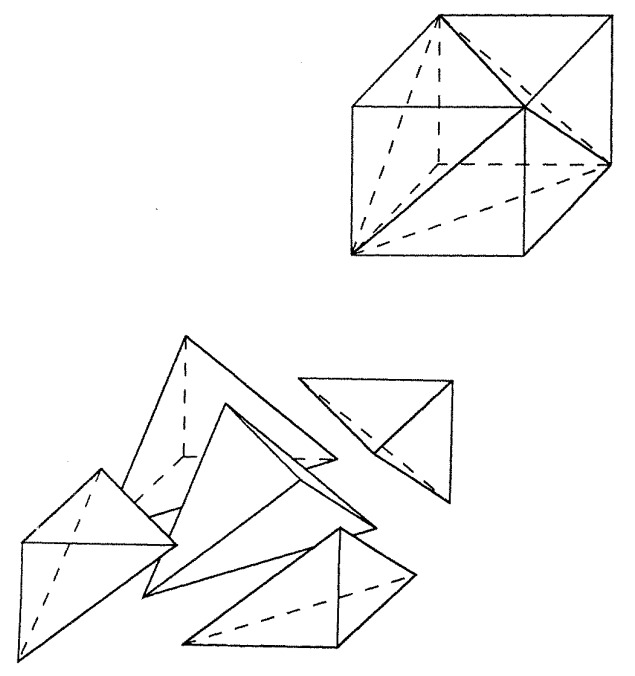
\includegraphics[width=7cm]{images/meshes/cube_division}\\
{\captionfont Decomposition of a hexahedron into five tetrahedra. Taken from \cite{begt92}.}
\end{center}

%............................................
\subsection{Hexahedra}

A hexahedron is a convex polytope isomorphic to the cube $[0,1]^3$.
Edges are line segments, facets are strictly {\bf planar} convex polygons.

\begin{center}
\includegraphics[width=5cm]{images/meshes/hexa.jpg}
\includegraphics[width=6cm]{images/meshes/hexa2}
\end{center}

\Literature Efficient Volume computation for Three- Dimensional hexahedral Cells \cite{duko88,gran97}

%.......................................
\subsection{Adaptive Mesh Refinement}
\index{general}{AMR} \index{general}{Adaptive Mesh Refinement}

Let us do a simple calculation and assume we wish to model mantle convection on Earth. 
The inner radius is $R_1=3485~\si{\km}$ and the bottom of the lithosphere is at $R_2=6250~\si{\km}$. 
The volume of fluid is then 
\[
V = \frac{4}{3}\pi (R_2^3-R_1^3) \simeq 8.5\times 10^{11}~\si{\km}^3
\]
Let us further assume that we are satisfied with an average resolution of $10~\si{\km}$. 
Each element/cell is then $10^3~\si{\km}^3$ and the total number of elements/cell is then 
\[
N \simeq 8.5 \times 10^8 \sim {\cal O}(10^9)
\]
This is a very large number. The resulting linear systems from the discretisation of the 
equations on such a mesh will be very even larger for the Stokes equations and solving 
these systems will require {\it very} large numbers of CPUs and long compute times. 

Aside from these considerations it is quite obvious that a high resolution mesh is not needed 
in parts of the mantle where large scale upwellings and downwellings occur, but 
probably even higher resolution will be needed in the vicinity of thin plumes and boundary layers. 
This means that a uniform mesh is a sub-optimal way of discretising space for such problems. 

The same reasoning also holds in the lithosphere where for instance narrow plate boundaries need to 
be adequately resolved while the inside of rigid plates can be modelled with coarser meshes. 

Finally, although one could employ meshing software to arrive at well balanced meshes in space, the 
dynamic character of the geodynamics modelling renders this approach cumbersome. A subduction zone, 
a mid-ocean rift or an ascending plume will evolve in time and the mesh will have to evolve in time too. 

In light of all this, it was only a matter of time before Adaptive Mesh Refinement was adopted 
in computatinal geodynamics. However, since the use and update of such meshes is somewhat 
complex in terms of numerical algorithms, its introduction came somewhat late (00's and later).
The \douar code (see Section~\ref{app:codes}) developed originally by J. Braun and Ph. Fullsack 
is a prime example of an early multi-purpose code relying on a self-written Octree library \cite{brtf08}.
More recently the \aspect{} code was developed on top of the Octree library p4est \cite{buwg11}.
Note the 2007 and 2008 papers by Davies et al \cite{dadh07,dadh08} which explore adaptive mesh 
refinement with the ConMan code (see Appendix~\ref{app:codes}).

For further reading I suggest you read the review by May, Schellart \& Moresi on this topic \cite{masm13}.

\begin{center}
\includegraphics[height=6cm]{images/meshes/bugg08.jpg}
\includegraphics[height=6cm]{images/meshes/bugg10.jpg}\\
{\captionfont Taken from \cite{bugg08} and \cite{bugg10}}
\end{center}

\begin{center}
\includegraphics[height=3.8cm]{images/meshes/gltf18.jpg}\\
{\captionfont Taken from \cite{gltf18}}
\end{center}

\Literature: 
\begin{itemize}
\item \fullcite{bugg08}
\item \fullcite{bugs09}
\item \fullcite{bugg10}
\item \fullcite{lezh11}
\item \fullcite{mish11}
\item \fullcite{svna18}
\item \fullcite{feba23}
\end{itemize}

\newpage
\paragraph{A short illustrative exercise}.

\input{amr_exercise}


%.......................................
\subsection{Conformal Mesh Refinement \label{ss:cmr}}
\index{general}{Conformal Mesh Refinement}

The quadtree/octree mesh refinement presented above is one option
when it comes to mesh refinement (or $h$-refinement). However their 
massive drawback is the presence of hanging notes which require 
special attention. 
Another approach to mesh refinement is conformal mesh refinement
as best exemplified on the following figures: 

\begin{center}
\includegraphics[height=4.5cm]{images/meshes/amrnew}\\
{\captionfont Taken from Deb \etal (1996) \cite{depl96}.
A typical instance of the outcome of the refinement procedure. 
Notice that the `spill-over' is reduced to one row on each side of the `localized' elements.}
\end{center}

\begin{center}
\includegraphics[height=4.5cm]{images/meshes/vaks15}
\includegraphics[height=4.5cm]{images/meshes/depl96}
\includegraphics[height=4.5cm]{images/meshes/habo04}\\
\includegraphics[height=4.5cm]{images/meshes/kott05}
\includegraphics[height=4.5cm]{images/meshes/specfem}\\
\includegraphics[height=4.5cm]{images/meshes/conf3D}\\
{\captionfont 
Top row, From left to right: 
van Driel \etal (2015) \cite{vaks15}; 
Deb \etal (1996) \cite{depl96}; 
Harris \etal (2004) \cite{habo04}; 
Komatitsch \etal (2005) \cite{kott05}; 
Middle row: Specfem manual;
Bottom row: I don't know anymore.}
\end{center}

\begin{center}
\includegraphics[height=5cm]{images/meshes/gari09_a}
\includegraphics[height=5cm]{images/meshes/gari09_b}\\
{\captionfont Taken from \textcite{gari09} (2009).}
\end{center}

\begin{center}
\includegraphics[height=4cm]{images/meshes/newmeshref1}
\includegraphics[height=4cm]{images/meshes/newmeshref2}
\end{center}


\begin{center}
\includegraphics[height=4cm]{images/meshes/refine_mesh_sheet_directional1}
\includegraphics[height=4cm]{images/meshes/refine_mesh_sheet_directional2}
\includegraphics[height=4cm]{images/meshes/refine_mesh_sheet_directional4}\\
\url{https://cubit.sandia.gov/public/14.0/help_manual/WebHelp/mesh_generation/mesh_modification/mesh_refinement.htm}
\end{center}

\Literature:
\begin{itemize}
\item D{\"u}ster \& Rank \cite{dura01},
\item Harris \etal (2004) \cite{habo04},
\item Anderson \etal (2009) \cite{anbo09},
\item Anderson \cite{ande09}, 
\item Garimella (2009) \cite{gari09},
\item Nicolas \& Fouquet (2013) \cite{nifo13,nifo13b}.
\item Parrish \cite{parr07}, 
\item Schneiders \cite{schn00,schn96,schn96b,schn99},
\item Schneiders \etal \cite{scde95},
\item Staten \& Canann \cite{stca97},
\item book by Ramm \etal \cite{rarr03}.
\end{itemize}

%.......................................
\subsection{Stretching the mesh}

In some cases the topology of the mesh can be regular but one can for instance stretch 
the mesh such that (for instance) the vertical resolution is higher at the top than at the bottom, 
or higher in the middle than on the sides.

The idea behind the transformation is a piecewise-linear function which maps [0,L] to [0,L] where 
$L$ is the length of the domain in the $x$-direction. For instance, this transformation can take the following form:

\begin{center}
\includegraphics[width=8cm]{images/meshes/stretching/stretch_towards_center}\\
{\captionfont Parameters $\beta_1$ and $\beta_2$ control the shape of the lines.\\ 
The kinks in the line occur at $\beta_1 L$ and $(1-\beta_1)L$ (see code here under).}
\end{center}

The (minimal) code to transform the mesh is as follows:
\begin{lstlisting}
def stretch_towards_center(x,L,beta1,beta2):
    if x<beta1*L: 
       val = beta2/beta1*x
    elif x<(1.-beta1)*L: 
       val = (1-2*beta2)/(1-2*beta1)*(x-beta1*L)+beta2*L
    else:
       val=beta2/beta1*(x-(1-beta1)*L)+(1-beta2)*L
    return val

[...]

beta1=0.25
beta2=0.375

for i in range(0,NV):
    x[i]=stretch_towards_center(x[i],Lx,beta1,beta2)
\end{lstlisting}

The following meshes count 64x16 elements. The top one is a regular mesh, with square elements, 
while the second one has been stretched by means of the transformation above:

\begin{center}
\includegraphics[width=8cm]{images/meshes/stretching/stretch_x}
\end{center}

Concerning the stretching towards the top of the model domain, the transformation line is as follows:

\begin{center}
\includegraphics[width=8cm]{images/meshes/stretching/stretch_towards_top}\\
{\captionfont Parameters $\beta_1$ and $\beta_2$ control the shape of the lines. The kinks in the 
line occur at $\beta_1 L$ and $(1-\beta_1)L$.\\ The slope of the left line is $\beta_2/\beta_1 x$.}
\end{center}

The (minimal) code to transform the mesh is as follows:
\begin{lstlisting}
def stretch_towards_top(x,L,beta1,beta2):
    if x<beta1*L: 
       val=beta2/beta1*x
    else:
       val=(1-beta2)/(1-beta1)*(x-beta1*L)+beta2*L
    return val

[...]

beta1=0.25
beta2=0.5
for i in range(0,NV):
    y[i]=stretch_towards_top(y[i],Ly,beta1,beta2)
\end{lstlisting}


The following meshes count 64x16 elements. The top one is a regular mesh, with square elements, 
while the second one has been stretched by means of the transformation above.
\begin{center}
\includegraphics[width=8cm]{images/meshes/stretching/stretch_y}
\end{center}

Finally both transformations can be applied to the same mesh:
\begin{center}
\includegraphics[width=8cm]{images/meshes/stretching/stretch_xy}
\end{center}

This approach is used in \stone 67.

%.......................................
\subsection{Meshes in an annulus}


\begin{center}
\includegraphics[width=6.8cm]{images/meshes/brhv08}
\includegraphics[width=6.8cm]{images/meshes/brva07a}\\
{\captionfont The quadratic finite element mesh as used in 
Brandenburg \etal \cite{brhv08,brva07a}}
\end{center}


%.......................................
\subsection{Meshes in/on a hollow sphere}

The following is for the most part published in Thieulot (2018) \textcite{thie18} (2018).

To a first approximation the Earth is a sphere: the Earth's polar diameter is 
about 43 kilometers shorter than its equatorial diameter, a negligible difference of 
about 0.3\%. As a consequence, modelling physical processes 
which take place in the planet require the discretisation of a sphere. 
Furthermore, because core dynamics occur on vastly difference time scales than mantle dynamics, mantle 
modelling usually leaves the core out, thereby requiring simulations to be run on a hollow sphere mesh
(with the noticeable exception of \textcite{geyu07}).

Although so-called latitude-longitude grids would seem appealing, 
they suffer from the convergence of meridians at the poles
(resulting in over sampling at poles) and the juxtaposition of triangles 
near the poles and quadrilaterals elsewhere. 
As a consequence more regular, but more complex, grids have been designed 
over the years which tesselate the surface of the 
sphere into triangles or quadrilaterals (sometimes overlapping).
There is the 'cubed sphere' \cite{roip96,heta03,chob05,sthh06,chcc07,brmw10,yiym19},
the Yin-Yang grid \cite{kasa04,yoka04,yoka06,kaks08,tack08,crta14,crta16},
the Yin-Yang-zhong grid \cite{haka16}, the Yin-yang grid of 
Shahnas \& Peltier \cite{shpe15}, the spiral grid \cite{hust08}, 
an icosahedron-based grid \cite{bafr85,malp02},
or a grid composed of 12 blocks further subdivided into quadrilaterals \cite{zhzm00} 
as used in the CitcomS code.
Note that \cite{oldp12} have also presented a method for generating a numerical 
grid on a spherical surface which 
allows the grid to be based on several different regular polyhedrons (including octahedron, 
cube, icosahedron, and rhombic dodecahedron). 
Ideally, one wishes to generate a mesh that is regular,
i.e. angles between edges/faces as close to $90^\circ$ as possible, 
of approximately similar volumes.


\begin{center}
\includegraphics[width=12cm]{images/meshes/kaks08}\\
{\captionfont Example of Yin-Yang grid. Taken from \textcite{kaks08} (2008).}
\end{center}

How such meshes are built is often not discussed in the literature. It is 
a tedious exercise of three-dimensional geometry and it can be time-consuming, especially 
the connectivity array generation. In Thieulot (2018) \cite{thie18} I present an open source 
mesh generator for three hollow sphere meshes: the 'cubed sphere' mesh, the CitcomS mesh and the 
icosahedral mesh:

\begin{itemize}
\item 
The cubed sphere ('HS06'), composed of 6 blocks which 
are themselves subdivided into $N_b \times N_b$ quadrilateral shaped cells  \cite{sado72,roip96,heta03,busa13}.
Four types of cubed spheres meshes have been proposed: the conformal, elliptic, gnomonic and spring types \cite{puli07}:


\begin{center}
\includegraphics[width=6.5cm]{images/meshes/puli07}
\includegraphics[width=8.5cm]{images/meshes/cubed_nair}\\
{\captionfont 
Left: The cubed-sphere grids at $2^\circ$ resolution displaying cells on the sphere,
 the image focuses on the distribution of grid cells near one corner of the grid;
 (a) conformal mapping \cite{rapm96,mcgr96}, (b) the gnomonic grid modified by elliptic solver,
 (c) equiangular gnomonic mapping and (d) the gnomonic grid modified by spring dynamics. \cite{puli07}.
Right: Taken from presentation by R. Nair, see Nair2008.pdf
}
\end{center}

However only gnomonic meshes are considered in Thieulot (2018): these 
are obtained by inscribing a cube within a sphere and expanding to the surface
of the sphere.
The cubed sphere has been used in large-scale mantle convection simulation in conjunction with 
Adaptive Mesh Refinement \cite{algs12,busa13}.  

\begin{center}
\includegraphics[width=4cm]{images/ghost/hs06}
\end{center}



\item 
The CitcomS mesh ('HS12') composed of 12 blocks also subdivided 
into $N_b \times N_b$ quadrilateral shaped cells
\cite{zhzm00,sthh06,zhmt08,arfw14}.
Note that \aspect{} \cite{krhb12,hedg17}, a relatively new code aimed at 
superseeding CitcomS can generate and use 
this type of mesh \cite{thie17} but is not limited to it.

\begin{center}
\includegraphics[width=4cm]{images/ghost/citcom12}
\end{center}


\item The icosahedral mesh ('HS20') composed of 20 triangular blocks \cite{bafr85,baum85} subdivided into triangles, which is 
used in the TERRA code \cite{burb96,burb97,burl98,dadb13}.
\end{itemize}


\begin{center}
\includegraphics[width=8cm]{images/meshes/spherical_choices1}
\includegraphics[width=8cm]{images/meshes/spherical_choices2}\\
{\captionfont source?}
\end{center}



Given the regularity and symmetry of these meshes determining the location of the 
mesh nodes in space is a relatively straightforward task. Building the mesh connectivity in an 
efficient manner is where the difficulty lies.

The approach to building all three meshes is identical:
\begin{enumerate}
\item A reference square or triangle is populated with cells,
parametrised by a level $l$: the square is subdivided into $l\times l$ quadrilaterals while 
the triangle is subdivided into $l^2$ triangles.
\begin{center}
\includegraphics[width=8cm]{images/ghost/f01_basics}\\
{\captionfont Reference square and triangles meshes at level 5.}
\end{center}

\item This reference square or triangle is then replicated {\sl nblock} times (6, 12 or 20) and mapped
onto a portion of a unit sphere. The blocks are such that their union covers a full sphere
but they cannot overlap except at the edges:
\begin{center}
\includegraphics[width=.8\linewidth]{images/ghost/f02}\\
{\captionfont From left to right: HS06, HS12 and HS20 shells coloured by block number.}
\end{center}

\item All block meshes are then merged together to generate a shell mesh. This task is rather 
complex as duplicate nodes must be removed and all connectivity arrays of the blocks must then 
be mended accordingly. 

\item Shell meshes are replicated {\sl nlayer+1} times outwards with increasing radii. 
The {\sl nlayer} shells are then merged together to form a hollow sphere mesh:
\begin{center}
\includegraphics[width=10cm]{images/ghost/f03_3HS}\\
{\captionfont a) HS06 mesh composed of 6 blocks containing each $6^3$ cells; 
b) HS12 mesh composed of 12 blocks containing each 
$6^3$ cells; e) HS20 mesh composed of 20 blocks containing each $6^3$ cells.}
\end{center}

\end{enumerate}



More information on these steps is available in the manual of the code.
In the following table the number of nodes and cells for a variety of resolutions 
for all three mesh types is reported. Looking at the CitcomS literature of the past 20 years, we find that 
the mesh data presented in this table cover the various resolutions used, e.g.
$12\times48^3$ \cite{mczh04,arfw14}, $12\times64^3$ \cite{budt14}
$12\times96^3$ \cite{bumb10}, $12\times128^3$ \cite{beck06,wele16,welm16}.
Note that in the case of the HS06 and HS12 meshes the mesh nodes are mapped out to the 6 or 12 blocks 
following either an equidistant or equiangle approach (see \cite{puli07}
for details on both approaches). 

\begin{center}
\begin{tabular}{lrrrl}
\hline
type & level & $N$ & $N_{el}$ & structure\\
\hline
\hline
HS06 & 
2   &  78        &  48         &$6\times 2^3$    \\
HS06 & 
4   &  490       &  384        &$6\times 4^3$    \\
HS06 & 
8   &  3,474      &  3,072       &$6\times 8^3$    \\
HS06 & 
16  &  26,146     &  24,576      &$6\times 16^3$    \\
HS06 & 
32  &  202,818    &  196,608     &$6\times 32^3$    \\
HS06 & 
64  &  1,597,570   &  1,572,864    &$6\times 64^3$    \\
HS06 & 
128 &  12,681,474  &  12,582,912   &$6\times 128^3$    \\
HS06 & 
256 &  101,057,026 &  100,663,296  &$6\times 256^3$    \\
\hline
HS12 & 2    &          150  &          96  &  $12\times 2^3$ \\
HS12 & 4    &          970  &         768  &  $12\times 4^3$ \\
HS12 & 8    &        6,930  &       6,144  &  $12\times 8^3$ \\
HS12 & 16   &       52,258  &      49,152  &  $12\times 16^3$ \\
HS12 & 32   &      405,570  &     393,216  &  $12\times 32^3$ \\
HS12 & 48   &    1,354,850  &   1,327,104  &  $12\times 48^3$ \\
HS12 & 64   &    3,195,010  &   3,145,728  &  $12\times 64^3$ \\
HS12 & 128  &   25,362,690  &  25,165,824  &  $12\times 128^3$ \\
HS12 & 256  &  202,113,538  & 201,326,592  &  $12\times 256^3$ \\
\hline
HS20 & 
2     &         126  &         160   & $20 \times 2^3$ \\
HS20 & 
4     &         810  &       1,280   & $20 \times 4^3$ \\
HS20 & 
8     &       5,778  &      10,240   & $20 \times 8^3$ \\
HS20 & 
16    &      43,554  &      81,920   & $20 \times 16^3$ \\
HS20 & 
32    &     337,986  &     655,360   & $20 \times 32^3$ \\
HS20 & 
64    &   2,662,530  &   5,242,880   & $20 \times 64^3$ \\
HS20 & 
128   &  21,135,618  &  41,943,040   & $20 \times 128^3$ \\
HS20 & 
256   & 168,428,034  & 335,544,320   & $20 \times 256^3$ \\
\hline
\end{tabular}\\
{\captionfont Number of nodes $N$ and elements/cells $N_{el}$ for the three types of meshes and for various 
levels.\\ HS06: cubed sphere; HS12: CitcomS mesh; HS20: icosahedral mesh.}
\end{center}

There are also many possibilities offered by the use of tetrahedral cells/elements:


\begin{center}
\includegraphics[height=4.5cm]{images/meshes/oebm09}
\includegraphics[height=4.5cm]{images/meshes/geotess}\\
{\captionfont Left: Grid of a global neo-tectonic SHELLS model coupled to a global mantle
circulation model; colours represent temperatures (red=hot, blue=cold)
at a depth of $200\si{km}$ below the surface. Taken from Oeser \etal (2009) \cite{oebm09}.
Right: Taken from the GeoTess software \footnote{\url{https://www.sandia.gov/geotess/}} manual.}
\end{center}


\begin{center}
\includegraphics[width=7cm]{images/meshes/htm}\\
{\captionfont Example of a Hierarchical Triangular Mesh}
\end{center}


\begin{center}
\includegraphics[width=7cm]{images/meshes/bafr85}
\includegraphics[width=7cm]{images/meshes/simj12}\\
{\captionfont \textcite{bafr85} (1985), \textcite{simj12} (2012)}
\end{center}


\Literature: 
\begin{itemize}
\item \textcite{phdo19} (2019) present an algorithm which builds 
polyhedral-based grids.
\item \textcite{upsm11} (2011) on icosahedral-hexagonal grids on 
a sphere for CFD applications.
\item \textcite{saku97} (1997) on distributing many points on a sphere.
\item \textcite{swpu06} (2006) on Fibonacci grids which possess virtually 
uniform and isotropic resolution, with an equal area for each grid point.
\item \textcite{hasa04} (2004) on discretizing manifolds via Minimum Energy Points.
Element Software
\end{itemize}


 %-----------------------------------
%\newpage %----------------------------------------------------------------------------------------
%\section{Visco-Plasticity} \input{viscoplasticity} %-------------------------------------------
\newpage %-----------------------------------------------------------------------------------------
\section{Pressure smoothing/filtering for $Q_1\times P_0$ elements \label{psmoothing}} \begin{flushright} {\tiny {\color{gray} \tt pressure\_smoothing.tex}} \end{flushright}
%~~~~~~~~~~~~~~~~~~~~~~~~~~~~~~~~~~~~~~~~~~~~~~~~~~~~~~~~~~~~~~~~~~~~~~~~~~~~~~~~~~~~~~~~~~~~~~~~~~

It has been widely documented that the use of the $Q_1 \times P_0$ element is 
not without problems. Aside from the 
consequences it has on the FE matrix properties, we will here focus on another unavoidable side effect: 
the spurious pressure checkerboard modes. 
\index{general}{Pressure Smoothing} 
\index{general}{Checkerboard mode}

These modes have been thoroughly analysed decades ago, see for instance
\textcite{hulb79} (1979), 
\textcite{sagl81a,sagl81b} (1981),
\textcite{grsi94} (1994).
They can be filtered out (\textcite{chpc95} (1995)) 
or simply smoothed (\textcite{legs79} (1979)), as we will see later.
Nodes on edges and corners may need special treatment as documented in \textcite{sagl81a} (1981) 
or \textcite{legs79} (1979).
The list of 8 schemes is not exhaustive with regards to the above mentioned publications. 
There has been considerable amount of work on the topic and this section is 
unfortunately not representing the literature appropriately.

On the following figure (a,b), pressure fields for the lid driven cavity experiment 
are presented for both an even and un-even number of elements. We see that 
the amplitude of the modes can sometimes be so large that the `real' pressure signal is 
not visible under the checkerboard and that something as simple as the number of elements in the 
domain can trigger those or not at all.

\begin{center}
a)\includegraphics[width=4cm]{images/checkerboard/p_el}
\includegraphics[width=4cm]{images/checkerboard/p_el_33x33}
b)\includegraphics[width=5cm]{images/checkerboard/press_doneahuerta}
c)\includegraphics[width=7cm]{images/checkerboard/douarpunch}\\
{\captionfont a) element pressure for a 32x32 grid and for a 33x33 grid;\\ 
b) image from \cite[p307]{dohu03} for a manufactured solution;
c) elemental pressure and smoothed pressure for the punch experiment \cite{thfb08}}
\end{center}

%----------------------------------------------------------------------
\subsection{Scheme 1}

The easiest post-processing step that can be used (especially when a regular grid is used) 
is explained in \textcite{thfb08} (2008): ``The element-to-node interpolation is performed by
averaging the elemental values from elements common to each node; 
the node-to-element interpolation is performed
by averaging the nodal values element-by-element. This
method is not only very efficient but produces a smoothing
of the pressure that is adapted to the local density of the
octree. Note that these two steps can be repeated until a
satisfying level of smoothness (and diffusion) of the pressure field is attained.''

\begin{center}
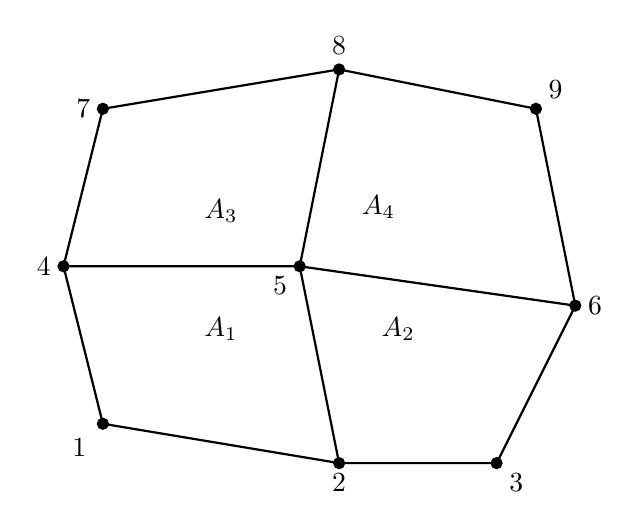
\begin{tikzpicture}
%\draw[fill=gray!5,gray!5](0,0) rectangle (9,7);
%\draw[step=0.5cm,gray,very thin] (0,0) grid (9,7); %background grid
\draw[thick](1.5,1.5) -- (4.5,1) -- (6.5,1) -- (7.5,3) -- (7,5.5) -- (4.5,6) --(1.5,5.5) -- (1,3.5) -- cycle;  
\draw[thick](4.5,1)--(4,3.5)--(4.5,6);
\draw[thick](1,3.5)--(4,3.5)--(7.5,3);
\draw[black,fill=black] (1.5,1.5) circle (2pt); \node[] at (1.2,1.2){1}; %1
\draw[black,fill=black] (4.5,1)   circle (2pt); \node[] at (4.5,0.75){2}; %2
\draw[black,fill=black] (6.5,1)   circle (2pt); \node[] at (6.75,0.75){3}; %3
\draw[black,fill=black] (1,3.5)   circle (2pt); \node[] at (0.75,3.5){4}; %4
\draw[black,fill=black] (4,3.5)   circle (2pt); \node[] at (3.75,3.25){5}; %5
\draw[black,fill=black] (7.5,3)   circle (2pt); \node[] at (7.75,3){6}; %6
\draw[black,fill=black] (1.5,5.5) circle (2pt); \node[] at (1.25,5.5){7}; %7
\draw[black,fill=black] (4.5,6)   circle (2pt); \node[] at (4.5,6.3){8}; %8
\draw[black,fill=black] (7,5.5)   circle (2pt); \node[] at (7.25,5.75){9}; %9
%\draw[thin,dashed](1,3.5)--(4.5,1)--(7.5,3)--(4.5,6)--cycle;
\node[] at (3,2.7){$A_1$}; %8
\node[] at (5.25,2.7){$A_2$}; %8
\node[] at (5,4.25){$A_4$}; %8
\node[] at (3,4.2){$A_3$}; %8
\end{tikzpicture}
\end{center}
\[
q_5^{(1)} = \frac{1}{4}\sum_{e=1}^4 p_e
\] 

In the codes which rely on the $Q_1 \times P_0$ element, the (elemental) pressure
is simply defined as 
\begin{lstlisting}
p=np.zeros(nel,dtype=np.float64)  
\end{lstlisting}
while the nodal pressure is then defined as\footnote{In virtually all stones $p$
stands for the 'raw' pressure and $q$ stands for its projection onto the velocity mesh.} 
\begin{lstlisting}
q=np.zeros(nnp,dtype=np.float64)  
\end{lstlisting}
The element-to-node algorithm is then simply (in 2D):

\begin{lstlisting}
count=np.zeros(nnp,dtype=np.int32)  
for iel in range(0,nel):
    q[icon[0,iel]]+=p[iel]
    q[icon[1,iel]]+=p[iel]
    q[icon[2,iel]]+=p[iel]
    q[icon[3,iel]]+=p[iel]
    count[icon[0,iel]]+=1
    count[icon[1,iel]]+=1
    count[icon[2,iel]]+=1
    count[icon[3,iel]]+=1
q=q/count
\end{lstlisting}

%----------------------------------------------------------------------
\subsection{Schemes 2,3}

{\sl Schemes 2,3} are very similar and are presented in \textcite{sagl81a,sagl81b} (1981).
Scheme 2 uses the areas of the surrounding elements as weights for the arithmetic averaging
while scheme 3 uses the area of the triangles:

\begin{multicols}{2}

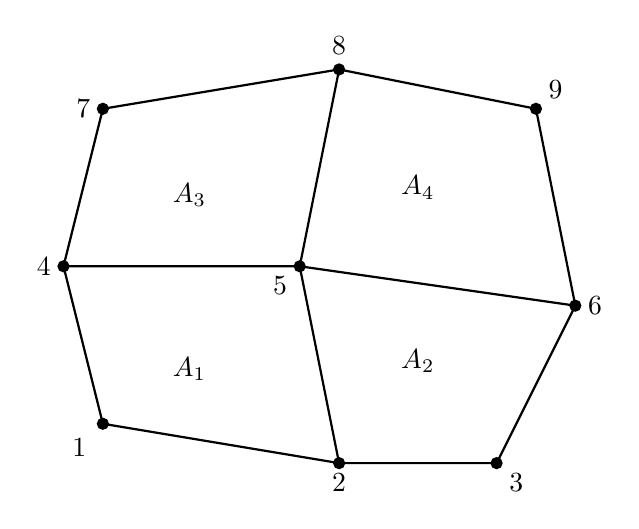
\begin{tikzpicture}
%\draw[fill=gray!5,gray!5](0,0) rectangle (9,7);
%\draw[step=0.5cm,gray,very thin] (0,0) grid (9,7); %background grid
\draw[thick](1.5,1.5) -- (4.5,1) -- (6.5,1) -- (7.5,3) -- (7,5.5) -- (4.5,6) --(1.5,5.5) -- (1,3.5) -- cycle;  
\draw[thick](4.5,1)--(4,3.5)--(4.5,6);
\draw[thick](1,3.5)--(4,3.5)--(7.5,3);
\draw[black,fill=black] (1.5,1.5) circle (2pt); \node[] at (1.2,1.2){1}; %1
\draw[black,fill=black] (4.5,1)   circle (2pt); \node[] at (4.5,0.75){2}; %2
\draw[black,fill=black] (6.5,1)   circle (2pt); \node[] at (6.75,0.75){3}; %3
\draw[black,fill=black] (1,3.5)   circle (2pt); \node[] at (0.75,3.5){4}; %4
\draw[black,fill=black] (4,3.5)   circle (2pt); \node[] at (3.75,3.25){5}; %5
\draw[black,fill=black] (7.5,3)   circle (2pt); \node[] at (7.75,3){6}; %6
\draw[black,fill=black] (1.5,5.5) circle (2pt); \node[] at (1.25,5.5){7}; %7
\draw[black,fill=black] (4.5,6)   circle (2pt); \node[] at (4.5,6.3){8}; %8
\draw[black,fill=black] (7,5.5)   circle (2pt); \node[] at (7.25,5.75){9}; %9
\node[] at (2.6,2.2){$A_1$}; %8
\node[] at (5.5,2.3){$A_2$}; %8
\node[] at (2.6,4.4){$A_3$}; %8
\node[] at (5.5,4.5){$A_4$}; %8
\end{tikzpicture}

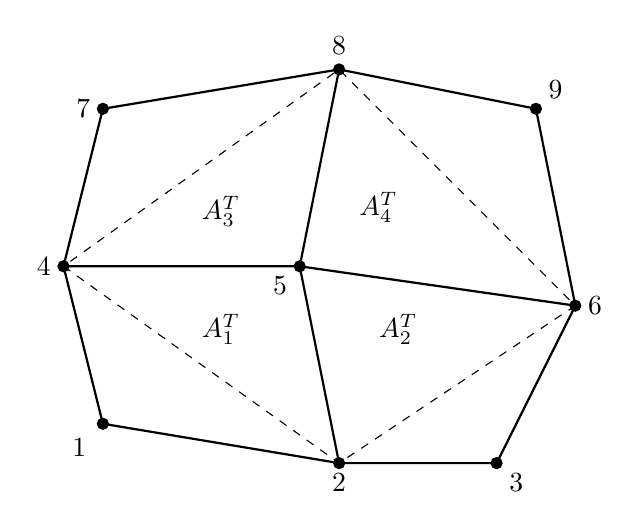
\begin{tikzpicture}
%\draw[fill=gray!5,gray!5](0,0) rectangle (9,7);
%\draw[step=0.5cm,gray,very thin] (0,0) grid (9,7); %background grid
\draw[thick](1.5,1.5) -- (4.5,1) -- (6.5,1) -- (7.5,3) -- (7,5.5) -- (4.5,6) --(1.5,5.5) -- (1,3.5) -- cycle;  
\draw[thick](4.5,1)--(4,3.5)--(4.5,6);
\draw[thick](1,3.5)--(4,3.5)--(7.5,3);
\draw[black,fill=black] (1.5,1.5) circle (2pt); \node[] at (1.2,1.2){1}; %1
\draw[black,fill=black] (4.5,1)   circle (2pt); \node[] at (4.5,0.75){2}; %2
\draw[black,fill=black] (6.5,1)   circle (2pt); \node[] at (6.75,0.75){3}; %3
\draw[black,fill=black] (1,3.5)   circle (2pt); \node[] at (0.75,3.5){4}; %4
\draw[black,fill=black] (4,3.5)   circle (2pt); \node[] at (3.75,3.25){5}; %5
\draw[black,fill=black] (7.5,3)   circle (2pt); \node[] at (7.75,3){6}; %6
\draw[black,fill=black] (1.5,5.5) circle (2pt); \node[] at (1.25,5.5){7}; %7
\draw[black,fill=black] (4.5,6)   circle (2pt); \node[] at (4.5,6.3){8}; %8
\draw[black,fill=black] (7,5.5)   circle (2pt); \node[] at (7.25,5.75){9}; %9
\draw[thin,dashed](1,3.5)--(4.5,1)--(7.5,3)--(4.5,6)--cycle;
\node[] at (3,2.7){$A_1^T$}; %8
\node[] at (5.25,2.7){$A_2^T$}; %8
\node[] at (5,4.25){$A_4^T$}; %8
\node[] at (3,4.2){$A_3^T$}; %8
\end{tikzpicture}

\end{multicols}

\[
q_5^{(2)} = \frac{\sum\limits_{e=1}^4 A_e p_e}{\sum\limits_{e=1}^4 A_e}
\qquad
\qquad
q_5^{(3)} = \frac{\sum\limits_{e=1}^4 A_e^T p_e}{\sum\limits_{e=1}^4 A_e^T}
\] 


\begin{remark} Although Schemes 1,2,3 are similar, scheme 1 is the simplest and fastest
to implement since the areas of neighbouring elements/triangles are not needed.
\end{remark}

\begin{remark} 
Schemes 1,2,3 are identical if all elements are rectangles of identical dimensions.
\end{remark}


%----------------------------------------------------------------------
\subsection{Scheme 4} 

This scheme has been designed by me. 
It resembles the last three ones, but the weighing is in this case different.

Let us consider a 1D problem:
\begin{center}
\includegraphics[width=0.5\linewidth]{images/pressure_smoothing/newalgo.png}
\end{center}

Elemental pressures $p_1$ and $p_2$ corresponding to elements 1 and 2 respectively are known at
locations $x_1$ and $x_2$. The two elements have a different size, characterised in this case
by the distances $d_1$ and $d_2$ to their common edge.

The equation of the line passing through points $(x_1,p_1)$ and $(x_2,p_2)$ is 
\[
p(x)=\frac{p_2-p_1}{x_2-x_1}(x-x_1)+p_1
\]
The $x$ coordinate of the common edge is given by $x=x_1+d_1/2$, 
and since $x_2-x_1=(d_1+d_2)/2$, the 
pressure at this location writes:
\[
p(x_M)= \frac{p_2-p_1}{d_1+d_2}d_1+p_1 = \frac{\frac{p_1}{d_1} + \frac{p_2}{d_2}}{\frac{1}{d_1} + \frac{1}{d_2}}
\]
Extrapolating this formula to 2D, $d_1$ and $d_2$ are in fact the element volumes, so that
\[
q_5^{(4)} = 
\frac{\sum\limits_{j=1}^4 \frac{p_j^e}{A_j^e}}{\sum\limits_{j=1}^4 \frac{1}{A_j^e}}
=
\frac{
\frac{p_1^e}{A_1^e}+
\frac{p_2^e}{A_2^e}+
\frac{p_3^e}{A_3^e}+
\frac{p_4^e}{A_4^e}
}{
\frac{1}{A_1^e}+
\frac{1}{A_2^e}+
\frac{1}{A_3^e}+
\frac{1}{A_4^e}
}\]

There remains a problem, due to the presence of the boundary nodes for which 
the sums present in the above equation do not run up to 4. A boundary
node only has three neighbours and a corner node only two. Additional measures
are required for these nodes. 

\begin{center}
\includegraphics[width=0.5\linewidth]{images/pressure_smoothing/newalgo_corner.png}
\end{center}

The pressure value $p_N$ is obtained as follows:
\[
q_N = \frac{ 
 \frac{p_2^e}   {A_2^e}
+\frac{p_3^e}   {A_3^e}
+\frac{p_{2'}^e}{A_{2'}^e}
+\frac{p_{3'}^e}{A_{3'}^e}
}{
 \frac{1}{A_2^e}
+\frac{1}{A_3^e}
+\frac{1}{A_{2'}^e}
+\frac{1}{A_{3'}^e}
}
\]
The areas and pressures of the mirrored elements 2' and 3' are extrapolated from the areas of elements 2 and 6, and 3 and 7 respectively. 
Likewise the pressure $p_M$ at the corner node is obtained through the pressures of its surrounding elements.


%------------------------------------------------------------------------------
\subsection{Scheme 5 - Least squares} 

This scheme is presented (among other places) in Lee \etal (1979)
\cite{legs79}. 
Let us start from the patch of 4 $Q_1$ elements counting 9 nodes: 

\begin{center}
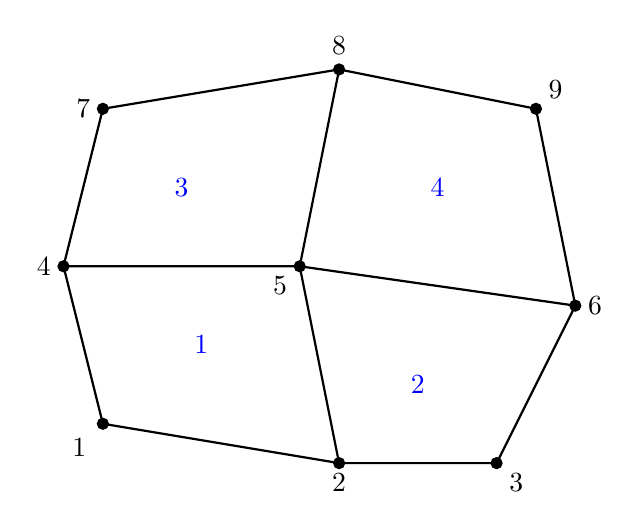
\begin{tikzpicture}
%\draw[fill=gray!5,gray!5](0,0) rectangle (9,7);
%\draw[step=0.5cm,gray,very thin] (0,0) grid (9,7); %background grid
\draw[thick](1.5,1.5) -- (4.5,1) -- (6.5,1) -- (7.5,3) -- (7,5.5) -- (4.5,6) --(1.5,5.5) -- (1,3.5) -- cycle;  
\draw[thick](4.5,1)--(4,3.5)--(4.5,6);
\draw[thick](1,3.5)--(4,3.5)--(7.5,3);

\node[] at (2.75,2.5) {\color{blue}1};
\node[] at (5.5,2) {\color{blue}2};
\node[] at (2.5,4.5) {\color{blue}3};
\node[] at (5.75,4.5) {\color{blue}4};

\draw[black,fill=black] (1.5,1.5) circle (2pt); \node[] at (1.2,1.2){1}; %1
\draw[black,fill=black] (4.5,1)   circle (2pt); \node[] at (4.5,0.75){2}; %2
\draw[black,fill=black] (6.5,1)   circle (2pt); \node[] at (6.75,0.75){3}; %3
\draw[black,fill=black] (1,3.5)   circle (2pt); \node[] at (0.75,3.5){4}; %4
\draw[black,fill=black] (4,3.5)   circle (2pt); \node[] at (3.75,3.25){5}; %5
\draw[black,fill=black] (7.5,3)   circle (2pt); \node[] at (7.75,3){6}; %6
\draw[black,fill=black] (1.5,5.5) circle (2pt); \node[] at (1.25,5.5){7}; %7
\draw[black,fill=black] (4.5,6)   circle (2pt); \node[] at (4.5,6.3){8}; %8
\draw[black,fill=black] (7,5.5)   circle (2pt); \node[] at (7.25,5.75){9}; %9

\end{tikzpicture}
\end{center}



We are looking for a field $q$ living on the nodes.
We build the quantity
\[
J=\iint_\Omega (q-p)^2 dV
\]
where $p$ is the elemental field. To make things clearer we split the integral into 
the sum of elemental integrals:
\[
J=
\iint_{\Omega_1} (q(x,y)-p_1)^2 dV+
\iint_{\Omega_2} (q(x,y)-p_2)^2 dV+
\iint_{\Omega_3} (q(x,y)-p_3)^2 dV+
\iint_{\Omega_4} (q(x,y)-p_4)^2 dV
\]
Inside each element the field $q(x,y)$ is given by a bilinear interpolation so that:
\begin{eqnarray}
J
&=& \iint_{\Omega_1} (\bN_1(x,y) q_1 + \bN_2(x,y)q_2 + \bN_5(x,y)q_5 + \bN_4(x,y)q_4 -p_1)^2 dV \nn\\
&+& \iint_{\Omega_2} (\bN_2(x,y) q_2 + \bN_3(x,y)q_3 + \bN_6(x,y)q_6 + \bN_5(x,y)q_5 -p_2)^2 dV \nn\\
&+& \iint_{\Omega_3} (\bN_4(x,y) q_4 + \bN_5(x,y)q_5 + \bN_8(x,y)q_8 + \bN_7(x,y)q_7 -p_3)^2 dV \nn\\
&+& \iint_{\Omega_4} (\bN_5(x,y) q_5 + \bN_6(x,y)q_6 + \bN_9(x,y)q_9 + \bN_8(x,y)q_8 -p_4)^2 dV 
\end{eqnarray}
where the $N_i$ functions are the basis functions (unusually expressed in $x,y$ coordinates).
The least square procedure looks for the set of $q_i$ such that 
\[
\frac{\partial J}{\partial q_i} =0 \qquad \forall i=1,...9
\]
and this yields 9 equations/constraints for 9 unknowns.
\begin{eqnarray}
\frac{\partial J}{\partial q_1} 
&=& \iint_{\Omega_1} 2 (\bN_1(x,y) q_1 + \bN_2(x,y)q_2 + \bN_5(x,y)q_5 + \bN_4(x,y)q_4 -p_1) \bN_1(x,y) dV \nn\\
\frac{\partial J}{\partial q_2}
&=& \iint_{\Omega_1} 2(\bN_1(x,y) q_1 + \bN_2(x,y)q_2 + \bN_5(x,y)q_5 + \bN_4(x,y)q_4 -p_1) \bN_2(x,y) dV \nn\\
&+& \iint_{\Omega_2} 2(\bN_2(x,y) q_2 + \bN_3(x,y)q_3 + \bN_6(x,y)q_6 + \bN_5(x,y)q_5 -p_2) \bN_2(x,y) dV \nn\\
\frac{\partial J}{\partial q_3}
&=& \iint_{\Omega_2} 2(\bN_2(x,y) q_2 + \bN_3(x,y)q_3 + \bN_6(x,y)q_6 + \bN_5(x,y)q_5 -p_2) \bN_3(x,y) dV \nn\\
\frac{\partial J}{\partial q_4}
&=& \iint_{\Omega_1} 2(\bN_1(x,y) q_1 + \bN_2(x,y)q_2 + \bN_5(x,y)q_5 + \bN_4(x,y)q_4 -p_1) \bN_4(x,y) dV \nn\\
&+& \iint_{\Omega_3} 2(\bN_4(x,y) q_4 + \bN_5(x,y)q_5 + \bN_8(x,y)q_8 + \bN_7(x,y)q_7 -p_3) \bN_4(x,y) dV \nn\\
\frac{\partial J}{\partial q_5}
&=& \iint_{\Omega_1} 2(\bN_1(x,y) q_1 + \bN_2(x,y)q_2 + \bN_5(x,y)q_5 + \bN_4(x,y)q_4 -p_1) \bN_5(x,y) dV \nn\\
&+& \iint_{\Omega_2} 2(\bN_2(x,y) q_2 + \bN_3(x,y)q_3 + \bN_6(x,y)q_6 + \bN_5(x,y)q_5 -p_2) \bN_5(x,y) dV \nn\\
&+& \iint_{\Omega_3} 2(\bN_4(x,y) q_4 + \bN_5(x,y)q_5 + \bN_8(x,y)q_8 + \bN_7(x,y)q_7 -p_3) \bN_5(x,y) dV \nn\\
&+& \iint_{\Omega_4} 2(\bN_5(x,y) q_5 + \bN_6(x,y)q_6 + \bN_9(x,y)q_9 + \bN_8(x,y)q_8 -p_4) \bN_5(x,y) dV \nn\\
\frac{\partial J}{\partial q_6}
&=& \iint_{\Omega_2} 2(\bN_2(x,y) q_2 + \bN_3(x,y)q_3 + \bN_6(x,y)q_6 + \bN_5(x,y)q_5 -p_2) \bN_6(x,y) dV \nn\\
&+& \iint_{\Omega_4} 2(\bN_5(x,y) q_5 + \bN_6(x,y)q_6 + \bN_9(x,y)q_9 + \bN_8(x,y)q_8 -p_4) \bN_6(x,y) dV \nn\\
\frac{\partial J}{\partial q_7}
&=& \iint_{\Omega_3} 2(\bN_4(x,y) q_4 + \bN_5(x,y)q_5 + \bN_8(x,y)q_8 + \bN_7(x,y)q_7 -p_3) \bN_7(x,y) dV \nn\\
\frac{\partial J}{\partial q_8}
&=& \iint_{\Omega_3} 2(\bN_4(x,y) q_4 + \bN_5(x,y)q_5 + \bN_8(x,y)q_8 + \bN_7(x,y)q_7 -p_3) \bN_8(x,y)dV \nn\\
&+& \iint_{\Omega_4} 2(\bN_5(x,y) q_5 + \bN_6(x,y)q_6 + \bN_9(x,y)q_9 + \bN_8(x,y)q_8 -p_4) \bN_8(x,y)dV \nn\\ 
\frac{\partial J}{\partial q_9}
&=& \iint_{\Omega_4} 2(\bN_5(x,y) q_5 + \bN_6(x,y)q_6 + \bN_9(x,y)q_9 + \bN_8(x,y)q_8 -p_4) \bN_9(x,y)dV 
\end{eqnarray}
The factor 2 are removed and the terms $\int p_i N_j $ are known so they end up in the right hand side.
\begin{eqnarray}
 \iint_{\Omega_1} (\bN_1 \bN_1 q_1 + \bN_1 \bN_2 q_2 + \bN_1 \bN_5 q_5 + \bN_1 \bN_4 q_4) dV 
&=& \iint_{\Omega_1} p_1 N_1 dV \nn\\
 \iint_{\Omega_1} (\bN_2 \bN_1 q_1 + \bN_2 \bN_2 q_2 + \bN_2 \bN_5 q_5 + \bN_2 \bN_4 q_4) dV \nn\\
+\iint_{\Omega_2} (\bN_2 \bN_2 q_2 + \bN_3 \bN_2 q_3 + \bN_6 \bN_2 q_6 + \bN_5 \bN_2 q_5) dV 
&=& \iint_{\Omega_1} p_1N_2 dV + \iint_{\Omega_2}  p_2 \bN_2 dV \nn\\
\nn\\
\dots &=& \dots \nn\\
\nn\\
 \iint_{\Omega_4} (\bN_9\bN_5 q_5 + \bN_9\bN_6q_6 + \bN_9\bN_9q_9 + \bN_9\bN_8q_8) dV &=&  \iint_{\Omega_4} p_4 \bN_9 dV 
\end{eqnarray}

The mass matrices corresponding to the four elements are 
\[
{\bm M}_1 = \int_{\Omega_1} \left( \begin{array}{cccc}
 \bN_1 \bN_1 & \bN_1 \bN_2 & \bN_1 \bN_5 & \bN_1 \bN_4 \\
 \bN_2 \bN_1 & \bN_2 \bN_2 & \bN_2 \bN_5 & \bN_2 \bN_4 \\
 \bN_5 \bN_1 & \bN_5 \bN_2 & \bN_5 \bN_5 & \bN_5 \bN_4 \\
 \bN_4 \bN_1 & \bN_4 \bN_2 & \bN_4 \bN_5 & \bN_4 \bN_4 
\end{array}\right) dV
\qquad
{\bm M}_2 = \int_{\Omega_2} \left( \begin{array}{cccc}
 \bN_2 \bN_2 & \bN_2 \bN_3 & \bN_2 \bN_6 & \bN_2 \bN_5 \\
 \bN_3 \bN_2 & \bN_3 \bN_3 & \bN_3 \bN_6 & \bN_3 \bN_5 \\
 \bN_6 \bN_2 & \bN_6 \bN_3 & \bN_6 \bN_6 & \bN_6 \bN_5 \\
 \bN_5 \bN_2 & \bN_5 \bN_3 & \bN_5 \bN_6 & \bN_5 \bN_5 
\end{array}\right) dV
\]
\[
{\bm M}_3 = \int_{\Omega_3} \left( \begin{array}{cccc}
 \bN_4 \bN_4 & \bN_4 \bN_5 & \bN_4 \bN_8 & \bN_4 \bN_7 \\
 \bN_5 \bN_4 & \bN_5 \bN_5 & \bN_5 \bN_8 & \bN_5 \bN_7 \\
 \bN_8 \bN_4 & \bN_8 \bN_5 & \bN_8 \bN_8 & \bN_8 \bN_7 \\
 \bN_7 \bN_4 & \bN_7 \bN_5 & \bN_7 \bN_8 & \bN_7 \bN_7 
\end{array}\right) dV
\qquad
{\bm M}_4 = \int_{\Omega_4} \left( \begin{array}{cccc}
 \bN_5 \bN_5 & \bN_5 \bN_6 & \bN_5 \bN_9 & \bN_5 \bN_8 \\
 \bN_6 \bN_5 & \bN_6 \bN_6 & \bN_6 \bN_9 & \bN_6 \bN_8 \\
 \bN_9 \bN_5 & \bN_9 \bN_6 & \bN_9 \bN_9 & \bN_9 \bN_8 \\
 \bN_8 \bN_5 & \bN_8 \bN_6 & \bN_8 \bN_9 & \bN_8 \bN_8 
\end{array}\right) dV
\]
so that the 9 equations above are actually the result of the assembly process of these four 
elemental systems:
\[
\left( \iint_{\Omega_e} \vec{\bN}^T\vec{\bN} dV \right) \cdot \vec{q}_e = \iint_{\Omega_i} \vec{\bN}^T p_e dV 
\qquad\qquad e=1,2,3,4
\]

Also check section 4.5.4 of \textcite{glte87} (1987), in which the authors 
present a two-step algorithm: 1) pressure is averaged over each element.
2) the nodal values of the pressure are recovered through a least-squares approach.


%------------------------------------------------------------------------------
\subsection{Scheme 6 - Consistent pressure recovery (penalty formulation) \label{ss:cpr}}

This is the method presented in \textcite{zina82} (1982). In the second part 
of this publication the authors wish to establish a simple and effective 
numerical method to calculate variables eliminated by the penalisation process. 
The method involves an additional finite element solution for the nodal 
pressures using the same finite element basis and numerical quadrature 
as used for the velocity.

Let us start with\footnote{I here voluntarily use $q$ instead of $p$}:
\[
q = -\lambda \vec\nabla\cdot \vec\upnu
\]
We are going to treat this equation like any other PDE in the context 
of the FE method, i.e. we are going to establish its weak form. 
We assume that the pressure is given inside an element by
\[
q(x,y) = \sum_{i=1}^{m_\upnu} \bN_i(x,y) q_i = \vec{\bN} \cdot \vec{q}
\]
and the velocity:
\[
\vec\upnu = (u,v) 
\qquad 
\qquad 
u(x,y)  = \sum_{i=1}^{m_\upnu} \bN_i(x,y) u_i
\qquad 
\qquad 
v(x,y)  = \sum_{i=1}^{m_\upnu} \bN_i(x,y) v_i
\]
where the $\bN_i$ are the $Q_1$ basis functions and $q_i$ are the sought after nodal values. 
We multiply the equation above by a $Q_1$ basis function $\bN_i$ and integrate over the whole domain:
\[
\iint_\Omega \bN_i(x,y) q(x,y) \; dxdy 
= -\lambda \iint_\Omega \bN_i \vec\nabla\cdot \vec\upnu  \; dx dy
\]
As before we now focus on the above expression inside a single element $e$:
\[
\iint_{\Omega_e} \bN_i(x,y) q(x,y) \; dxdy = -\lambda \iint_{\Omega_e} \bN_i \vec\nabla\cdot \vec\upnu \; dx dy
\]
After $\bN_i \rightarrow \vec{\bN}=(\bN_1,\bN_2,\bN_3,\bN_4)^T$, the left hand side term becomes:
\[
\iint _{\Omega_e} \vec{\bN}^T q(x,y) \; dxdy 
=
\iint _{\Omega_e} \vec{\bN}^T \vec{\bN} \cdot \vec{q} \; dxdy 
=
\left(\underbrace{\iint _{\Omega_e} \vec{\bN}^T \vec{\bN} dxdy}_{{\bm M}_e} \right) \cdot \vec{q}  
\]
where ${\bm M}_e$ is the elemental mass matrix.
We now turn to the right hand side. We have
\[
\vec\nabla\cdot \vec\upnu
= \frac{\partial u}{\partial x}+\frac{\partial v}{\partial y}
= \sum_i \frac{\partial \bN_i}{\partial x} u_i + \sum_i \frac{\partial \bN_i}{\partial y} v_i 
\]
We here too define $\vec{V}_e=(u_1,v_1,u_2,v_2,u_3,v_3,u_4,v_4)^T$ so that 

\begin{eqnarray}
&& \iint_{\Omega_e} \vec{\bN} {\vec \nabla}\cdot {\vec \upnu} \; dV \nn\\
&=& \iint_{\Omega_e} \vec{\bN}^T \sum_{i=1}^{m_\upnu} 
\left( \frac{\partial \bN_i}{\partial x} u_i + \frac{\partial \bN_i}{\partial y} v_i 
\right)  
dV \label{eq:psmoth6}\\
&=& 
\iint_{\Omega_e} 
\left(
\begin{array}{c}
\bN_1 \left(
\sum\limits_{i=1}^{4} \frac{\partial \bN_i}{\partial x} u_i +
\sum\limits_{i=1}^{4} \frac{\partial \bN_i}{\partial y} v_i \right) \\
\bN_2 \left(
\sum\limits_{i=1}^{4} \frac{\partial \bN_i}{\partial x} u_i +
\sum\limits_{i=1}^{4} \frac{\partial \bN_i}{\partial y} v_i \right) \\
\bN_3 \left(
\sum\limits_{i=1}^{4} \frac{\partial \bN_i}{\partial x} u_i +
\sum\limits_{i=1}^{4} \frac{\partial \bN_i}{\partial y} v_i \right) \\
\bN_4 \left(
\sum\limits_{i=1}^{4} \frac{\partial \bN_i}{\partial x} u_i +
\sum\limits_{i=1}^{4} \frac{\partial \bN_i}{\partial y} v_i \right) 
\end{array}
\right) dV \nonumber \\  %%%%%%%%%%%%%%%%%%%%%%%%%%
&=& 
\int_{\Omega_e} 
\left(
\begin{array}{ccc}
{\bN}_1& {\bN}_1 &  0 \\\\
{\bN}_2& {\bN}_2 &  0 \\\\
{\bN}_3& {\bN}_3 &  0 \\\\
{\bN}_4& {\bN}_4 &  0 
\end{array}
\right)
\cdot
\left(
\begin{array}{c}
\sum\limits_i \frac{\partial \bN_i}{\partial x} u_i \\ \\
\sum\limits_i \frac{\partial \bN_i}{\partial y} v_i \\ \\
\sum\limits_i (\frac{\partial \bN_i}{\partial y} u_i\! +\! \frac{\partial \bN_i}{\partial x} v_i) 
\end{array}
\right)
\; dV \nonumber\\ %%%%%%%%%%%%%%%%%%%%%%%%%%
&=& 
\int_{\Omega_e} 
\underbrace{
\left(
\begin{array}{cccccc}
{\bN}_1 & {\bN}_1 &  0 \\
{\bN}_2 & {\bN}_2 &  0 \\
{\bN}_3 & {\bN}_3 &  0 \\
{\bN}_4 & {\bN}_4 &  0 
\end{array}
\right)
}_{{\bm N}}
\cdot
\underbrace{
\left(\begin{array}{cccccccc}
\partial_x \bN_1 & 0 &  
\partial_x \bN_2 & 0 &  
\partial_x \bN_3 & 0 &  
\partial_x \bN_4 & 0 \\ \\
0 & \partial_y \bN_1 &   
0 & \partial_y \bN_2 &   
0 & \partial_y \bN_3 &   
0 & \partial_y \bN_4 \\ \\
\partial_y \bN_1 & \partial_x \bN_1 &  
\partial_y \bN_2 & \partial_x \bN_2 &  
\partial_y \bN_3 & \partial_x \bN_3 &  
\partial_y \bN_4 & \partial_x \bN_4 
\end{array}\right)}_{{\bm B}}
\cdot \vec{V}_e
\; dV  \nonumber \\
&=& 
\left(\int_{\Omega_e} {\bm N} \cdot {\bm B} \; dV \right) \cdot \vec{V}_e \nonumber\\
&=& -\G_e^T \cdot {\vec V}_e
\end{eqnarray}
This makes sense since $\G^T$ is the discrete divergence operator. However, it is not very efficient to 
build $\G_e$ only to multiply it with a vector of already known quantities. 
In practice we implement Eq.~\eqref{eq:psmoth6} which implmentation resembles the buoyancy term of the 
Stokes equation.

After assembly we arrive at
\[
{\bm M} \cdot \vec{q} = \lambda \G^T \cdot {\vec V} 
\qquad
\text{with}
\qquad
\G_e = -\int_{\Omega_e} {\bm N} \cdot {\bm B} \; dV
\]
where ${\bm M}$ is the global mass matrix, $\vec{q}$ the vector of all 
nodal pressures, $\G$ the discrete gradient matrix and $\vec{V}$
the (velocity) solution vector. 
The system can be easily solved since the mass matrix is a friendly matrix.
The vector ${\vec q}$ contains the nodal pressure values directly, with 
no need for a smoothing scheme! 

\begin{remark}
Very importantly, the mass matrix ${\bm M}$ is to be evaluated at the full integration points, 
while the constraint part (the right hand side of the equation) is to be evaluated at 
the reduced integration point, i.e. in the middle of the element.  
\end{remark}

\begin{remark}
As noted in \cite{zina82}, it is interesting to note that when linear elements are used 
and the lumped matrices are used for the ${\bm M}$ the resulting algebraic equation is identical 
to the smoothing scheme 1 only if a uniform square finite element 
mesh is used. In this respect this method is expected to yield different results when elements 
are not square or even rectangular.
\end{remark}

\begin{remark}
The third column of the matrix ${\bm N}$
and the last line of the ${\bm B}$ matrix could be removed altogether.
If your code is based on the mixed formulation, then you already 
have built matrix $\G$ so you can easily re-use this piece of code 
to compute $\G$ again, this time with a reduced integration quadrature.
If you are using the penalty formulation then you need to program 
all from scratch and then simply do away with these unnecessary terms, or 
you can direcly build the rhs as $\int_{\Omega_e} \vec{\bN}^T p_e$ (assuming
you have previously computed the pressure in the middle of each element 
by means of $p=-\lambda\vec\nabla\cdot\vec\upnu$).
\end{remark}

\begin{remark}
This  scheme is identical to the least square scheme!
\end{remark}


%--------------------------------------------------------------
\subsection{Scheme 7}

Same as scheme 6, but with lumped mass matrix.  


%--------------------------------------------------------------
\subsection{Scheme 8 - bilinear interpolation} 

Let us assume that the centers of the 
four elements make a $Q_1$ quadrilateral element, as shown on this figure:

\input{tikz/tikz_pscheme8}

The values at the corners are $p_1$,
$p_2$, $p_3$ and $p_4$. Assuming that the pressure inside this element 
can be represented by a bilinear field, we have 
\[
p(x,y)= a+ bx +cy +dxy
\]
where the coefficients will be determined by ensuring that 
$p(x_i,y_i)=p_i$ for $i=1,2,3,4$, or:
\begin{eqnarray}
a+bx_1+cy_1+dx_1y_1 &=& p_1 \\
a+bx_2+cy_2+dx_2y_2 &=& p_2 \\
a+bx_3+cy_3+dx_3y_3 &=& p_3 \\
a+bx_4+cy_4+dx_4y_4 &=& p_4 
\end{eqnarray}
i.e.
\[
\left(
\begin{array}{cccc}
1 & x_1 & y_1 & x_1y_1 \\
1 & x_2 & y_2 & x_2y_2 \\
1 & x_3 & y_3 & x_3y_3 \\
1 & x_4 & y_4 & x_4y_4
\end{array}
\right)\cdot
\left(
\begin{array}{c}
a \\b\\c\\d
\end{array}
\right)
=
\left(
\begin{array}{c}
p_1\\p_2\\p_3\\p_4
\end{array}
\right)
\]

There remains an issue with nodes which are on the boundaries of the 
domain. These are of course not 'surrounded' by four pressure values 
so the above algorithm does not apply directly. However, looking 
at the above figure, and assuming that node 1 is a lower left corner 
of a 2D domain, we can use the bilinear interpolation based on elements 
1,2,3,4 to extrapolate a nodal pressure value at node 1. 
The same would apply for nodes 2 and 4 for example. 

\begin{remark}
This scheme is not applicable to quadtree-based meshed.
\end{remark}





\newpage %-----------------------------------------------------------------------------------------
\section{Pressure scaling \label{pscaling}} \index{general}{pressure scaling}
\begin{flushright} {\tiny {\color{gray} pressure\_scaling.tex}} \end{flushright}
%~~~~~~~~~~~~~~~~~~~~~~~~~~~~~~~~~~~~~~~~~~~~~~~~~~~~~~~~~~~~~~~~~~~~~~~~~~~~~~~~~~~~~~~~~~~~~~~~~~

As nicely explained in the 
step 32 of deal.ii\footnote{\url{https://www.dealii.org/9.0.0/doxygen/deal.II/step\_32.html}},
we often need to scale the $\G$ block since it is many orders of magnitude smaller than $\K$ (especially in geodynamics where viscosities are $\sim 10^{22}$), 
which introduces large inaccuracies in the solving process to the point that the solution is nonsensical. 
This scaling coefficient is $\eta/L$ where $\eta$ and $L$ are representative viscosities and lengths. 
We start from 
\[
\left(
\begin{array}{cc}
\K & \G \\ \G^T & -\C 
\end{array}
\right)
\cdot
\left(
\begin{array}{c}
\vec{\cal V} \\ \vec{\cal P}
\end{array}
\right)
=
\left(
\begin{array}{c}
\vec{f} \\ \vec{h}
\end{array}
\right)
\]
and introduce the scaling coefficient as follows (which in fact does not alter the solution at all):
\[
\left(
\begin{array}{cc}
\K & \frac{\eta}{L}\G \\ \frac{\eta}{L}\G^T & - \frac{\eta^2}{L^2} \C 
\end{array}
\right)
\cdot
\left(
\begin{array}{c}
\vec{\cal V} \\\frac{L}{\eta} \vec{\cal P}
\end{array}
\right)
=
\left(
\begin{array}{c}
 \vec{f} \\ \frac{\eta}{L} \vec{h}
\end{array}
\right)
\]
We then end up with the modified Stokes system:
\[
\left(
\begin{array}{cc}
\K & \underline{\G} \\ \underline{\G}^T & \underline{\C} 
\end{array}
\right)
\cdot
\left(
\begin{array}{c}
\vec{\cal V} \\ \underline{\vec{\cal P}}
\end{array}
\right)
=
\left(
\begin{array}{c}
\vec{f} \\ \underline{\vec{h}}
\end{array}
\right)
\]
where 
\[
\underline{\G}=\frac{\eta}{L}\G
\quad\quad
\quad\quad
\underline{\vec{\cal P}}=\frac{L}{\eta} \vec{\cal P}
\quad\quad
\quad\quad
\underline{\C}=\frac{\eta^2}{L^2} \C
\quad\quad
\quad\quad
\underline{\vec{h}}=\frac{\eta}{L}\vec{h}
\]
After the solve phase, we recover the real pressure with $\vec{\cal P}=\frac{\eta}{L}\underline{\vec{\cal P}}$.





 %--------------------------
\newpage %-----------------------------------------------------------------------------------------
\section{Pressure normalisation, nullspace\label{ss_pnorm}} \begin{flushright} {\tiny {\color{gray} pressure\_normlisation.tex}} \end{flushright}
%~~~~~~~~~~~~~~~~~~~~~~~~~~~~~~~~~~~~~~~~~~~~~~~~~~~~~~~~~~~~~~~~~~~~~~~~~~~~~~~~~~~~~~~~~~~~~~~~~~


%..................................................
\subsubsection{Basic idea and naive implementation}

When Dirichlet boundary conditions are imposed everywhere on the boundary, 
pressure is only present by its gradient in 
the equations. It is thus determined up to an arbitrary constant (one speaks then 
of a nullspace of size 1).  \index{general}{Nullspace}
In such a case, one commonly impose the average of the pressure over the whole domain or on 
a subset of the boundary 
to have a zero average, i.e.
\begin{equation}
\int_\Omega p\; dV = 0
\end{equation}

Let us assume for example/simplicity that we are using \QonePzero elements. The pressure is constant 
inside each element so the integral above becomes:
\begin{equation}
\int_\Omega p\; dV = 
\sum_e  \int_{\Omega_e} p\; dV = 
\sum_e  p_e \int_{\Omega_e}\; dV = 
\sum_e  p_e V_e = 0
\end{equation}
where the sum runs over all elements $e$ of volume $V_e$.
This can be rewritten 
\[
\vec{L} \cdot \vec{\cal P}=0
\] 
and it is a constraint on the pressure solution which couples {\it all} pressure dofs. 
We can associate to it a Lagrange multiplier $\lambda$ so that we must solve the modified Stokes system:
\[
\left(
\begin{array}{ccc}
\K & \G & 0\\ 
\G^T & 0 & \vec{L}^T \\
0 & \vec{L} & 0
\end{array}
\right)
\cdot
\left(
\begin{array}{c}
\vec{\cal V} \\ \vec{\cal P} \\ \lambda
\end{array}
\right)
=
\left(
\begin{array}{c}
\vec{f} \\ \vec{h} \\ 0
\end{array}
\right)
\]
When higher order spaces are used for pressure (continuous or discontinuous)
one must then carry out the above integration numerically by means of (usually)
a Gauss-Legendre quadrature.

Although valid, this approach has one main disadvantage: it makes the Stokes matrix larger (although
marginally so -- only one row and column are added), but more importantly it prevents the use of some
of the solving strategies of Section \ref{sec:solvers}.


%..................................................
\subsubsection{Implementation -- the real deal}

Here is what Bochev and Gunzburger \cite[Section 7.6.4]{bogu09} have to say about this:
"[...] practical implementations cheat by substituting enforcement of the true zero mean constraint by using
procedures collectively known as setting the pressure datum. These procedures essentially 
amount to removing one degree of freedom from the pressure space.
Setting the pressure datum can be accomplished in many different ways, ranging
from specifying a pressure value at a grid node to more complicated approaches in
which a boundary traction is specified at a single node in lieu of the velocity condition; 
see [16, 24, 191] and the references cited therein for more details. Not surprisingly, 
in practice, the simplest approach of fixing the pressure value at a node also
happens to be the most widely used in practice."




The idea is actually quite simple and requires two steps:
\begin{enumerate}
\item remove the null space by prescribing the pressure at one location and solve the system;
\item post-process the pressure so as to arrive at a pressure field which fulfils the required normalisation (surface, volume, ...)
\end{enumerate}

The reason why it works is as follows: a constant pressure value lies in the null space, so that one can 
add or delete any value to the pressure field without consequence. As such I can choose said constant such that 
the pressure at a given node/element is zero. All other computed pressures are then relative to that one. 
The post-processing step will redistribute a constant value to all pressures (it will shift them up or down)
so that the normalising condition is respected. 


\Literature

In \url{https://scicomp.stackexchange.com/questions/27645/pressure-boundary-condition-in-lid-driven-cavity-using-finite-element-method}
we find:
{\it 
Zero mean pressure space is used for convenience when one is interested in FEA theory (basically, we cannot 
enforce $p(x_0)=p_0$ for $p \in L^2$ since it does not make sense); from the computational point of view, 
it is easier to fix one of the pressure DOFs (although you can subtract mean value at the post–processing step 
if you want to). When you are working w/ polynomial spaces—and this is exactly what you do in FEM 
-it is perfectly fine to enforce $p(x_0)=p_0$. Handle this constraint like you usually handle Dirichlet 
BCs (e.g., via modifying your matrix). It is also fine to ignore this constraint in some 
cases (e.g., Krylov solvers can do fine with this).
}


\url{
https://scicomp.stackexchange.com/questions/25134/mixed-finite-element-method-for-the-stokes-system-some-implementation-details}





 %----
\newpage %-----------------------------------------------------------------------------------------
\section{Solving the Stokes system \label{sec:solvers}} \begin{flushright} {\tiny {\color{gray} solvers.tex}} \end{flushright}
%~~~~~~~~~~~~~~~~~~~~~~~~~~~~~~~~~~~~~~~~~~~~~~~~~~~~~~~~~~~~~~~~~~~~~~~~~~~~~~~~~~~~~~~~~~~~~~~~~~

Let us start again from the (full) Stokes system:
\begin{equation}
\underbrace{
\left(
\begin{array}{cc}
\K & \G \\ \G^T & -\C 
\end{array}
\right)
}_{\cal A}
\cdot
\left(
\begin{array}{c}
\vec{\cal V} \\ \vec{\cal P}
\end{array}
\right)
=
\left(
\begin{array}{c}
\vec{f} \\ \vec{h}
\end{array}
\right)
\label{StokesSyst}
\end{equation}
We need to solve this system in order to obtain the solution, i.e. the $\vec{\cal V}$ 
and $\vec{\cal P}$ vectors. But how? 
Unfortunately, this question is not simple to answer and the appropriate method depends on many 
parameters, but mainly on how big the matrix blocks are and what the condition number of the matrix $\K$ is. 

First let us start with an obvious question: couldn't we just compute the inverse of the matrix ${\cal A}$?
Under the assumption that the inverse of $\K$ and $\SSS$ exists, we can and we find\footnote{The matrix 
$\C$ is here omitted but it bears no consequences on the conclusion.}
\[
{\cal A}^{-1} = 
\left(
\begin{array}{cc}
\K & \G \\ \G^T & 0
\end{array}
\right)^{-1}
=
\left(
\begin{array}{cc}
\K^{-1} + \K^{-1} \cdot \G \cdot\SSS^{-1} \cdot\G^T \cdot\K^{-1} & -\K^{-1} \cdot\G \cdot\SSS^{-1} \\ 
-\SSS^{-1} \cdot\G^T \cdot\K^{-1}  &  \SSS^{-1}
\end{array}
\right)
\]
However, such an expression is of limited interest in the numerical solution of saddle
point problems since it showcases 5 times the inverse of $\K$ and more importantly
the inverse of the Schur complement matrix $\S$ which is likely to be a full matrix so 
that we never want to compute it explicitely.


As concisely explained in Clevenger \& Heister (2021) \cite{clhe21}, 
there are three common approaches used in the literature for solving the above equation on large scales:
\begin{itemize}
\item a pressure corrected, Schur complement CG scheme, using multigrid as an 
approximation to the velocity block;
\item a block-preconditioned Krylov
method, also using multigrid on the velocity block.
For this method, there are two main types:
\begin{itemize}
\item GMRES\cite{mabl15,rumi15} (or any Krylov method not requiring symmetry) with
block-triangular preconditioner (This is what \aspect does):
\[
{\bm P} = \left(
\begin{array}{cc}
\K & \G \\
0 & - \SSS
\end{array}
\right)
\]

\item MINRES\cite{gmhj16} with block-diagonal preconditioner
\[
{\bm P} = \left(
\begin{array}{cc}
\K & 0 \\
0 & - \SSS
\end{array}
\right)
\]

\end{itemize}


\item an all-at-once multigrid performed on the entire Stokes
system, using Uzawa-type smoothers.
\end{itemize}


\Literature: Preconditioners for Incompressible Navier-Stokes Solvers \cite{seuv10}

Saddle point preconditioners have been extensively discussed and studied \cite{bewa08}, \cite{dewu04}

Diagonal preconditioners in \cite{shrb01}, \cite{babc94}.

Pragmatic solvers for 3D Stokes problems with heterogeneous coefficients \cite{samb20}

%...................................................
\subsection{When using the penalty formulation}

In this case we are only solving for 
velocity since pressure has been eliminated and is later recovered in a post-processing step:
\[
(\K_\eta+\K_\lambda) \cdot \vec {\cal V} = \vec f
\]
 We also know that 
the penalty factor $\lambda$ is many orders of magnitude higher than the viscosity and 
in combination with the use of the $Q_1 \times P_0$ element the resulting matrix 
condition number is very high so that the use of iterative solvers is precluded. 
Indeed codes such as \sopale \cite{full95}, \douar \cite{brtf08}, \fantom \cite{thie11} 
or \sulec \cite{qube11} relying on the penalty formulation all use direct solvers.
The most popular are BLKFCT\footnote{\url{http://dm.unife.it/blkfclt/}}, 
MUMPS\footnote{\url{http://mumps.enseeiht.fr/}}\cite{amdu89,amdl00,amdk01,amgl06,ambl19}, 
PasTiX \cite{herr02},
WSMP\footnote{\url{http://www.research.ibm.com/projects/wsmp}} \cite{GUPTA94ieee,GUPTA09sc-long},
UMFPACK and CHOLMOD\footnote{\url{http://faculty.cse.tamu.edu/davis/suitesparse.html}}
, SuperLU\footnote{\url{https://portal.nersc.gov/project/sparse/superlu/}}, 
PARDISO\footnote{\url{https://www.pardiso-project.org/}}
\cite{pardiso-6.0a,pardiso-6.0b,pardiso-6.0c}, or those inside 
PETSc\footnote{\url{https://www.mcs.anl.gov/petsc/}}.

Braun \etal (2008) \cite{brtf08} list the following features of direct solvers:
\begin{itemize}
\item Robust
\item Black-box operation
\item Difficult to parallelize
\item Memory consumption
\item Limited scalability
\end{itemize}

The main advantage of direct solvers is used in this case: They can solve ill-conditioned 
matrices. However, memory requirements for the storage of number of nonzeros in the 
Cholesky matrix grow very fast as the number of equations/grid size increases, especially in 3D,
to the point that even modern computers with tens of Gb of RAM cannot deal with a $\sim 100^3$ element mesh.
This explains why direct solvers are often used for 2D problems and rarely in 3D with noticeable 
exceptions \cite{thfb08,yahb09,brya10,lobh10,alht11,alht12,alhf13,whbb14,neew18}. 

%....................................................................
\subsection{Uzawa algorithms and the Schur complement approach }

\index{general}{Uzawa algorithm}

Let us write the above system as two equations:
\begin{eqnarray}
\K \cdot \vec{\cal V} + \G \cdot \vec{\cal P} &=& \vec{f} \\
\G^T \cdot  \vec{\cal V} - \C \cdot \vec{\cal P} &=& \vec{h} 
\end{eqnarray}
The first line can be re-written 
$\vec{\cal V}=\K^{-1}\cdot (\vec{f} - \G \cdot \vec{\cal P})$ and can be inserted in the second:
\begin{equation}
\G^T\cdot \vec{\cal V} =\G^T \cdot  [ \K^{-1} \cdot  (\vec{f} - \G \cdot  \vec{\cal P}) ] - \C\cdot \vec{\cal P} = \vec{h} 
\end{equation}
or, 
\begin{mdframed}[backgroundcolor=blue!5]
\begin{equation}
(\G^T \cdot \K^{-1} \cdot \G + \C) \cdot \vec{\cal P} = \G^T \cdot \K^{-1}\cdot \vec{f} - \vec{h} 
\end{equation}
\end{mdframed}
The matrix $\SSS= \G^T \cdot \K^{-1} \cdot \G + \C$ is called the Schur complement. 
\index{general}{Schur Complement} 
It is Symmetric (since $\K$ is symmetric) and  Positive-Definite\footnote{$M$ 
positive definite $\iff$ $x^TMx>0$ $\forall \; x\in \mathbb{R}^n \setminus {\bm 0}$ }
(SPD) \index{general}{SPD} if $Ker({\G})=0$. 
Having solved this equation (i.e. we have obtained $\vec{\cal P}$), the velocity can be recovered by solving 
$\K\cdot \vec{\cal V} =\vec{f}- \G \cdot \vec{\cal P}$. 

\begin{remark}
The Schur complement matrix naturally occurs when the Stokes matrix is decomposed using 
a LDU block-factorisation. Indeed, we have 
\[
\left(
\begin{array}{cc}
\K & \G \\ 
\G^T & 0
\end{array}
\right)
=
\left(
\begin{array}{cc}
{\bm I} & 0 \\ 
\G^T \cdot \K^{-1} & {\bm I}
\end{array}
\right)
\cdot
\left(
\begin{array}{cc}
\K & 0 \\ 
0 & -\SSS
\end{array}
\right)
\cdot
\left(
\begin{array}{cc}
{\bm I} & \K^{-1} \cdot \G \\ 
0 & {\bm I}
\end{array}
\right)
\]
\end{remark}

For now, let us assume that we have built the $\SSS$ matrix\footnote{We will 
revisit this topic later on, but be aware that we never build $\SSS$ in practice.} 
and the right hand 
side $\underline{\vec{f}}=\G^T \cdot \K^{-1} \cdot \vec{f} - \vec{h}$.
We must solve $\SSS\cdot \vec{\cal P} = \underline{\vec{f}}$.
It is easy to see that $\SSS$ is actually a full matrix (i.e. not sparse) and 
aside from the costs of building it explicitly using a direct solver would require 
a lot of memory so that we must then turn to iterative methods. 

\index{general}{Richardson Iterations}
One can resort to so-called Richardson iterations, defined as follows 
(e.g., see Varga \cite{varga}, p141):
in solving the matrix equation ${\bm A}\cdot {\vec X}={\vec b}$,
the Richardson iterative method is defined by: 
\begin{equation}
{\vec X}_{k+1} = {\vec X}_k + \alpha_k (-{\bm A} \cdot {\vec X}_k + {\vec b})
\quad\quad
m\geq 0 
\end{equation}
where the $\alpha_k$'s are real scalars. 
It is easy to see that when the method converges then ${\vec X}_{k+1} \simeq {\vec X}_k$  and then 
for $\alpha_k\neq 0$ then ${\bm A}\cdot {\vec X}={\vec b}$ is satisfied. 
In our case, it writes:
\begin{eqnarray}
\vec {\cal P}_{k+1} 
&=& \vec {\cal P}_{k} + \alpha_k ( - \SSS \cdot \vec{\cal P}_{k}  +  \underline{\vec{f}}) \nonumber\\
&=& \vec {\cal P}_{k} + \alpha_k \left[ - (\G^T \cdot \K^{-1} \cdot \G + \C)  \cdot \vec{\cal P}_{k} 
+  (\G^T \cdot \K^{-1} \cdot \vec{f} - \vec{h}   ) \right] \nonumber\\
&=& \vec {\cal P}_{k} + \alpha_k \left[ \G^T \cdot \K^{-1} \cdot ( - \G \cdot \vec{\cal P}_{k} + \vec{f}) 
-\C \cdot \vec{\cal P}_{k} - \vec{h} 
\right] \nonumber\\
&=& \vec {\cal P}_{k} + \alpha_k \left[ \G^T \cdot \K^{-1} \cdot ( \K\cdot \vec{\cal V}_k)
-\C \cdot \vec{\cal P}_{k}  - \vec{h} \right] \nonumber\\
&=& \vec {\cal P}_{k} + \alpha_k \left( \G^T \cdot \vec{\cal V}_k -\C \cdot \vec{\cal P}_{k} - \vec{h} \right) 
\end{eqnarray}
The above iterations are then carried out and for each new pressure field the associated velocity field 
is computed. The method of using Richardson iterations applied to the Schur complement 
is commonly called the Uzawa algorithm (see Braess \cite[p221]{braess}
\footnote{I have slightly 
altered the indices of the velocities wrt the book}).

\begin{mdframed}[backgroundcolor=blue!5]
\underline{\bf Uzawa algorithm (1)}: assume $\vec{\cal P}_0$ known
\begin{eqnarray}
\text{solve} \qquad \mathbb{K} \cdot \vec{\cal V}_k &=& \vec f - \mathbb{G}\cdot \vec {\cal P}_{k} \\
\vec{\cal P}_{k+1} &=& 
\vec{\cal P}_{k}  + \alpha_k (\mathbb{G}^T\cdot \vec{\cal V}_k  -\C \cdot \vec{\cal P}_{k} -\vec h)
\quad
\quad
\quad
\quad
k=0,1,2, ... \label{uzaa2}
\end{eqnarray}
\end{mdframed}


This method is rather simple to implement, although
what makes an appropriate set of $\alpha_k$ values is not straightforward, which is why 
the conjugate gradient is often preferred, as detailed in the next section. 

It is known that such iterations will converge for $0< \alpha < \rho(\SSS)= \lambda_{max}(\SSS)$ 
where $\rho(\SSS)$ is the spectral radius of the matrix $\SSS$
which is essentially the largest, in absolute value, eigenvalue of $\SSS$ (neither of which 
can be computed easily).  
It can also be proven that the rate of convergence depends on the condition number of the matrix.

Richardson iterations are part of the family of stationary iterative 
methods\footnote{\url{https://mathworld.wolfram.com/StationaryIterativeMethod.html}}, 
since it can be rewritten 
\begin{equation}
{\vec X}_{k+1} = ({\bm I} - \alpha_k {\bm A} ) \cdot {\vec X}_k + \alpha_k {\vec b}
\end{equation}
which is the definition of a stationary method. 
The four main stationary methods are the Jacobi method, 
Gauss-Seidel method, successive overrelaxation method (SOR), 
and symmetric successive overrelaxation method (SSOR)
\index{general}{Jacobi Iterative Method}
\index{general}{Gauss-Seidel Iterative Method}
\index{general}{SOR Iterative Method}
\index{general}{SSOR Iterative Method}


Since the $\alpha$ parameter is the key to a successful Uzawa algorithm, 
this issue has of course been looked into. What follows is 
presented in p221 of Braess \cite{braess}.
For the analysis of the Uzawa algorithm, we define the residue
\[
\vec {\cal R}_k = \vec h - \mathbb{G}^T \cdot \vec{\cal V}_k  +\C \cdot \vec{\cal P}_{k}
\]
In addition, suppose the solution of the saddle point problem is denoted
by $(\vec{\cal V}^\star,\vec{\cal P}^\star)$ so that we have
\[
\vec{f} = \K \cdot \vec{\cal V}^\star + \G \cdot \vec{\cal P}^\star
\qquad
{\rm and}
\qquad
\vec{h} = \G^T \cdot \vec{\cal V}^\star - \C \cdot \vec{\cal P}^\star 
\]

Now substituting the iteration formula for ${\cal V}_k$, and inserting $\vec{f}$ and $\vec{h}$ from above,
we get
\begin{eqnarray}
\vec{\cal R}_k 
&=& \vec{h} -\G^T  \cdot \vec{\cal V}_k  +\C \cdot \vec{\cal P}_{k} \nn\\
&=& \vec{h} -\mathbb{G}^T\cdot \mathbb{K}^{-1} (\vec f - \mathbb{G}\cdot \vec{\cal P}_{k})  +\C \cdot \vec{\cal P}_{k}\\
&=& (\G^T\cdot\vec{\cal V}^\star - \C \cdot \vec{\cal P}^\star) -\mathbb{G}^T\cdot \mathbb{K}^{-1} (\K\cdot\vec{\cal V}^\star 
+ \G\cdot\vec{\cal P}^\star - {\G}\cdot \vec{\cal P}_{k})+\C \cdot \vec{\cal P}_{k} \\
&=& ({\G}^T \cdot \mathbb{K}^{-1} \cdot \mathbb{G} + \C)\cdot (\vec {\cal P}_{k} - \vec{\cal P}^\star) 
\end{eqnarray}
From Eq.~\eqref{uzaa2} it follows that:
\begin{eqnarray}
\vec{\cal P}_{k+1} - \vec{\cal P}_{k}  
&=& \alpha\; (\mathbb{G}^T\cdot \vec{\cal V}_k -\C \cdot \vec{\cal P}_{k} -\vec h) \\
&=& -\alpha\; \vec{\cal R}_k \\ 
&=& -\alpha\; ( \mathbb{G}^T \cdot \mathbb{K}^{-1} \cdot \mathbb{G} + \C )
\cdot (\vec {\cal P}_{k} -\vec{\cal P}^\star)\\ 
&=& \alpha\; (\mathbb{G}^T \cdot \mathbb{K}^{-1} \cdot \mathbb{G} + \C) \cdot 
(\vec{\cal P}^\star - \vec {\cal P}_{k} ) 
\end{eqnarray}
Thus the Uzawa algorithm is equivalent to applying the gradient method 
to the reduced equation using a fixed step size. 
In particular, the iteration converges for
$
\alpha < 2 || \G^T \cdot \K^{-1} \cdot \G + \C||^{-1}
$
and one can show that the good step size $\alpha_k$ is given by 
\begin{equation}
\alpha_k = \frac{\vec{\cal R}_k \cdot \vec{\cal R}_k}
{(\G \cdot \vec{\cal R}_k)\cdot (\K^{-1}\cdot \G \cdot \vec{\cal R}_k)}
\label{uzaa3}
\end{equation}
\todo[inline]{include matrix $\C$!}


However, if we were to use this rule formally, we would 
need an additional multiplication by $\K^{-1}$ in every step 
of the iteration. This can be avoided by storing an 
auxiliary vector. 
Note that this algorithm is presented in Zienkiewicz \etal (1985) \cite{zivt85} 
in the context of viscoplastic flow.

%Note that in \cite{glow} it is stated: the convergence of this algorithm is proved for 
%$\alpha \in (0,2\mu/d)$ (where $d$ is the number of dimensions).
%\todo[inline]{check this, and report page number}

As mentioned above, there is a way to rework the original Uzawa algorithm 
to include Eq. (\ref{uzaa3}). It is yields a modified 
Uzawa algorithm (see p222 of Braess \cite{braess}
\footnote{I have slightly 
altered the indices of the velocities wrt the book}):


\begin{mdframed}[backgroundcolor=blue!5]
\underline{\bf Uzawa algorithm (2)}: assume $\vec{\cal P}_0$ known. 
Solve $\mathbb{K}\cdot \vec{\cal V}_0 = \vec f - \mathbb{G}\cdot  \vec{\cal P}_0$. 
For $k=0,1,2,...$, compute 
\begin{eqnarray}
\vec{\cal R}_k=\vec q_k &=& \vec h-\mathbb{G}^T \cdot \vec{\cal V}_k + \C \cdot \vec{\cal P}_{k}\\
\vec{p}_k &=& {\G}\cdot q_k \\
\vec H_k &=& {\K}^{-1}\cdot \vec{p}_k \\
\alpha_k &=& \frac{\vec q_k \cdot \vec q_k}{\vec{p}_k \cdot \vec H_k} \\
\vec {\cal P}_k &=& \vec {\cal P}_{k-1} - \alpha_k  \vec q_k \\
\vec {\cal V}_{k} &=& \vec {\cal V}_{k-1} + \alpha_k  \vec H_k
\end{eqnarray}
\end{mdframed}


\Literature: Cahouet \& Chabard (1988) \cite{cach88}, Cao (2003) \cite{cao03}.





%...................................................
\subsection{Conjugate gradient and the Schur complement approach }
\label{ss:schurpcg}

\index{general}{CG} \index{general}{Conjugate Gradient}
Since the Schur matrix $\SSS$ is Symmetric Positive Definite, 
the Conjugate Gradient (CG) method\footnote{\url{https://en.wikipedia.org/wiki/Conjugate_gradient_method}} \cite{hest52} 
is very appropriate to solve this system. 

Indeed, looking at the definition of Wikipedia: "{\it In mathematics, the conjugate gradient method is an algorithm 
for the numerical solution of particular systems of linear equations, namely those whose matrix is symmetric and positive-definite. 
The conjugate gradient method is often implemented as an iterative algorithm, applicable to sparse systems that are too large 
to be handled by a direct implementation or other direct methods such as the Cholesky decomposition. 
Large sparse systems often arise when numerically solving partial differential equations or optimization problems.}"

A simple Google search tells us that the Conjugate Gradient algorithm is as follows:

\begin{minipage}{0.40\textwidth}
\centering
{\captionfont Algorithm as obtained from Wikipedia.}\\
\frame{\includegraphics[width=7cm]{images/solvers/cgwiki}}
\end{minipage}\hfill
\begin{minipage}{0.50\textwidth}
The same algorithm with our notations:\\
$\vec{r}_0 = \underline{\vec{f}} - \SSS \cdot \vec{\cal P}_0$\\
$\vec{p}_0 = \vec{r}_0$\\
$k=0$ \\
repeat\\
\hspace{8mm} $\alpha_k = (\vec{r}_k^T\cdot \vec{r}_k )/(\vec{p}_k^T \cdot \SSS\cdot  \vec{p}_k )$\\
\hspace{8mm} $\vec{\cal P}_{k+1} = \vec{\cal P}_k+\alpha_k \vec{p}_k$\\
\hspace{8mm} $\vec{r}_{k+1} = \vec{r}_k - \alpha_k \; \SSS \cdot \vec{p}_k $ \\
\hspace{8mm} $\beta_k=(\vec{r}_{k+1}^T \cdot \vec{r}_{k+1})/(\vec{r}_k^T \cdot \vec{r}_k)$ \\
\hspace{8mm} $\vec{p}_{k+1} =\vec{r}_{k+1}+ \beta_k \vec{p}_k$ \\
$k=k+1$ \\
end repeat\\
return $\vec{\cal P}_{k+1}$ as the result
\end{minipage}

\vspace{.5cm}

This algorithm is of course explained in detail in many textbooks such as Saad \cite{saad},
in Zhong, Yuen, Moresi \& Knepley (2012) \cite{zhym12}, and in Section~\ref{ss:itsolvers}.

Let us look at this algorithm more closely. The parts which may prove to be somewhat tricky 
are those involving the matrix the Schur complement matrix since we wish never to build 
it explicitely. We start the iterations with a guess pressure $\vec{\cal P}_0$ (and an initial guess velocity 
which could be obtained by 
solving $\K\cdot \vec{\cal V}_0 =\vec{f}- \G\cdot \vec{\cal P}_0$).
\begin{eqnarray}
\vec{r}_0 
&=& \underline{\vec{f}}-\SSS \cdot \vec{\cal P}_0 \\
&=& \G^T\cdot \K^{-1}\cdot \vec{f} - \vec{h} - (\G^T\cdot \K^{-1}\cdot \G + \C)\cdot \vec{\cal P}_0 \\ 
&=& \G^T\cdot \K^{-1}\cdot (\vec{f} - \G\cdot \vec{\cal P}_0) - \vec{h} \\
&=& \G^T\cdot \K^{-1}\cdot \K\cdot \vec{\cal V}_0 -\C \cdot \vec{\cal P}_0 - \vec{h} \\ 
&=& \G^T\cdot \vec{\cal V}_0  -\C \cdot \vec{\cal P}_0   - \vec{h} 
\end{eqnarray}
We see that we were able to compute $\SSS \cdot \vec{\cal P}_0$ without ever forming the 
Schur complement matrix explicitely. We now turn to the $\alpha_k$ coefficient:
\[
\alpha_k 
= \frac{\vec{r}_k^T\cdot \vec{r}_k }{\vec{p}_k \cdot \SSS\cdot  \vec{p}_k } 
= \frac{\vec{r}_k^T \cdot \vec{r}_k }{\vec{p}_k\cdot (\G^T \cdot \K^{-1} \cdot \G +\C )\cdot \vec{p}_k } 
= \frac{\vec{r}_k^T \cdot \vec{r}_k }{(\G\cdot \vec{p}_k)^T \cdot  \K^{-1} \cdot (\G \cdot \vec{p}_k) + \vec{p}_k\cdot \C\cdot \vec{p}_k } 
\]
We then define $\tilde{\vec{p}}_k = \G \cdot \vec{p}_k$, so that $\alpha_k$ can be computed as follows:
\begin{enumerate}
\item compute $\tilde{\vec{p}}_k = \G \cdot  \vec{p}_k$
\item solve $\K\cdot  \vec{d}_k = \tilde{\vec{p}}_k$
\item compute 
\[
\alpha_k=\frac{\vec{r}_k^T \cdot \vec{r}_k}{\tilde{\vec{p}}_k^T \cdot \vec{d}_k 
+ \vec{p}_k\cdot^T \C\cdot \vec{p}_k }
\]
\end{enumerate}
Then we need to look at the term $\SSS\cdot \vec{p}_k$:
\[
\SSS\cdot \vec{p}_k = (\G^T\cdot \K^{-1}\cdot \G\cdot +\C )\vec{p}_k 
= \G^T\cdot \K^{-1}\cdot \tilde{\vec{p}}_k  + \C\cdot \vec{p}_k= \G^T\cdot  \vec{d}_k + \C \cdot \vec{p}_k
\]
We can then rewrite the CG algorithm as follows: 
\begin{itemize}
\item choose $\vec{\cal P}_0$
\item compute $\vec{\cal V}_0$ solution of $\K\cdot \vec{\cal V}_0 =\vec{f}- \G\cdot \vec{\cal P}_0$ 
\item $\vec{r}_0 = \G^T\cdot \vec{\cal V}_0 - \C \cdot \vec{\cal P}_0 - \vec{h}$ 
\item if $\vec{r}_0$ is sufficiently small, then return $(\vec{\cal V}_0,\vec{\cal P}_0)$ as the result
\item $\vec{p}_0=\vec{r}_0$
\item $k=0$
\item repeat
\begin{itemize}
\item compute $\tilde{\vec{p}}_k = \G\cdot \vec{p}_k$
\item solve $\K\cdot  \vec{d}_k = \tilde{\vec{p}}_k$
\item compute $\alpha_k=(\vec{r}_k^T \cdot  \vec{r}_k)/
              (\tilde{\vec{p}}_k^T\cdot \vec{d}_k + \vec{p}_k^T\cdot \C\cdot\vec{p}_k)$
\item $\vec{\cal P}_{k+1} = \vec{\cal P}_k+\alpha_k \vec{p}_k$
\item $\vec{r}_{k+1} = \vec{r}_k - \alpha_k (\G^T \cdot \vec{d}_k + \C \cdot \vec{p}_k) $
\item if $\vec{r}_{k+1}$ is sufficiently small, then exit loop
\item $\beta_k=(\vec{r}_{k+1}^T \cdot \vec{r}_{k+1})/(\vec{r}_k^T \cdot \vec{r}_k)$
\item $\vec{p}_{k+1} =\vec{r}_{k+1}+ \beta_k \vec{p}_k$
\item $k=k+1$
\end{itemize}
\item return $\vec{\cal P}_{k+1}$ as result
\end{itemize}
We see that we have managed to solve the Schur complement equation with the Conjugate Gradient method
without ever building the matrix $\SSS$. Having obtained the pressure solution $\vec{\cal P}_{k+1}$, 
we can easily recover 
the corresponding velocity with $\K\cdot \vec{\cal V}_{k+1} =\vec{f}- \G\cdot \vec{\cal P}_{k+1}$. 
However, this is rather unfortunate because it requires yet another solve with the $\K$ matrix. 
As it turns out, we can slightly alter the above algorithm to have it update the velocity 
as well so that this last solve is unnecessary.

We have 
\begin{eqnarray}
\vec{\cal V}_{k+1} 
&=& \K^{-1}\cdot (f - \G\cdot \vec{\cal P}_{p+1} )\\
&=& \K^{-1}\cdot (f - \G\cdot (\vec{\cal P}_k+\alpha_k \vec{p}_k) ) \\
&=& \K^{-1}\cdot (f - \G\cdot \vec{\cal P}_k) - \alpha_k \K^{-1}\cdot \G \cdot \vec{p}_k \\
&=& \vec{\cal V}_k - \alpha_k \K^{-1}\cdot \tilde{\vec{p}}_k  \\
&=& \vec{\cal V}_k - \alpha_k \vec{d}_k 
\end{eqnarray}
and we can insert this minor extra calculation inside the algorithm and get the velocity solution 
nearly for free. The final CG algorithm is then 

\begin{mdframed}[backgroundcolor=blue!5]
\underline{\bf solver\_cg}: assume $\vec{\cal P}_0$ known
\begin{itemize}
\item compute $\vec{\cal V}_0=\K^{-1}\cdot (\vec{f}-\G \cdot \vec{\cal P}_0)$
\item $\vec{r}_0 = \G^T\cdot \vec{\cal V}_0 -\C \cdot \vec{\cal P}_0 - \vec{h}$ 
\item if $\vec{r}_0$ is sufficiently small, then return $(\vec{\cal V}_0,\vec{\cal P}_0)$ as the result
\item $\vec{p}_0=\vec{r}_0$
\item $k=0$
\item repeat
\begin{itemize}
\item compute $\tilde{\vec{p}}_k = \G \cdot \vec{p}_k$
\item solve $\K\cdot \vec{d}_k = \tilde{p}_k$
\item compute $\alpha_k=(\vec{r}_k^T \cdot  \vec{r}_k)/(\tilde{\vec{p}}_k^T \cdot \vec{d}_k 
      + \vec{p}_k^T \cdot \C\cdot \vec{p}_k)$
\item $\vec{\cal P}_{k+1} = \vec{\cal P}_k+\alpha_k \vec{p}_k$
\item $ \vec{\cal V}_{k+1} = \vec{\cal V}_k - \alpha_k \vec{d}_k$
\item $\vec{r}_{k+1} = \vec{r}_k - \alpha_k (\G^T \cdot \vec{d}_k + \C \cdot \vec{p}_k) $
\item if $\vec{r}_{k+1}$ is sufficiently small ($||\vec{r}_{k+1}||_2/||\vec{r}_0||_2 <tol$), then exit loop
\item $\beta_k=(r_{k+1}^T r_{k+1})/(r_k^T r_k)$
\item $\vec{p}_{k+1} =\vec{r}_{k+1}+ \beta_k \vec{p}_k$
\item $k=k+1$
\end{itemize}
\item return $\vec{\cal P}_{k+1}$ as result
\end{itemize}
\end{mdframed}

\begin{remark}
The matrix $\C$ is rarely present unless for example when stabilised elements are used 
such as the stabilised $Q_1\times P_0$ or the stabilised $Q_1\times Q_1$ elements.
\end{remark}

This iterative algorithm will converge to the solution with a rate which depends on 
the condition number of the $\SSS$ matrix, which is not easy to compute since 
$\SSS$ is never built. However, it has been established that large viscosity contrasts in the domain 
will have a negative impact on the convergence. 

\begin{remark} 
This algorithm requires one solve with matrix $\K$ per iteration 
but says nothing about the method employed to do so (direct or iterative solver)
nor the corresponding preconditioner.
\end{remark} 

\index{general}{Preconditioned Conjugate Gradient}  
One thing we know improves the convergence of any iterative solver is the use of a 
preconditioner matrix and therefore now focus on the Preconditioned Conjugate Gradient (PCG) method.
Once again we turn to Wikipedia\footnote{\url{https://en.wikipedia.org/wiki/Conjugate_gradient_method}}:

\begin{minipage}{0.40\textwidth}
\centering
{\captionfont Algorithm as obtained from Wikipedia.}\\
\frame{\includegraphics[width=7cm]{images/solvers/pcgwiki}}
\end{minipage}\hfill
\begin{minipage}{0.50\textwidth}
The same algorithm with our notations:\\
$\vec{r}_0 = \underline{\vec{f}} - \SSS \cdot \vec{\cal P}_0$\\
$\vec{z}_0= {\bm M}^{-1} \cdot \vec{r}_0$ \\
$\vec{p}_0 = \vec{z}_0$\\
$k=0$ \\
repeat\\
\hspace{8mm} $\alpha_k = (\vec{r}_k^T\cdot \vec{z}_k )/(\vec{p}_k^T \cdot \SSS\cdot  \vec{p}_k )$\\
\hspace{8mm} $\vec{\cal P}_{k+1} = \vec{\cal P}_k+\alpha_k \vec{p}_k$\\
\hspace{8mm} $\vec{r}_{k+1} = \vec{r}_k - \alpha_k \; \SSS \cdot \vec{p}_k $ \\
\hspace{8mm} $\vec{z}_{k+1} = {\bm M}^{-1} \cdot \vec{r}_{k+1}$ \\
\hspace{8mm} $\beta_k=(\vec{z}_{k+1}^T \cdot \vec{r}_{k+1})/(\vec{z}_k^T \cdot \vec{r}_k)$ \\
\hspace{8mm} $\vec{p}_{k+1} =\vec{z}_{k+1}+ \beta_k \vec{p}_k$ \\
$k=k+1$ \\
end repeat\\
return $\vec{\cal P}_{k+1}$ as the result
\end{minipage}

\vspace{.5cm}

Unsurprisingly we find the same algorithm in Saad \cite{saad}:

\frame{\includegraphics[width=7cm]{images/solvers/saad}}

Note that in the algorithm above the preconditioner matrix ${\bm M}$ 
has to be symmetric positive-definite and fixed, i.e., cannot change from iteration to iteration. 
We see that this algorithm introduces an additional vector $\vec{z}$ and a solve with the 
matrix ${\bm M}$ at each iteration, which means that ${\bm M}$ must 
be such that solving ${\bm M}\cdot \vec{x}= \vec{f}$ 
where $\vec{f}$ is a given rhs vector must be cheap. Ultimately, the PCG algorithm applied to 
the Schur complement equation takes the form:

\begin{mdframed}[backgroundcolor=blue!5]
\underline{\bf solver\_pcg}: assume $\vec{\cal P}_0$ known
\begin{itemize}
\item compute ${\cal V}_0=\K^{-1}(f-\G{\cal P}_0)$
\item $\vec{r}_0 = \G^T {\cal V}_0 - \C \cdot \vec{\cal P}_0 - \vec{h}$
\item if $\vec{r}_0$ is sufficiently small, then return $(\vec{\cal V}_0,\vec{\cal P}_0)$ as the result
\item $\vec{z}_0= M^{-1} \cdot \vec{r}_0$ 
\item $\vec{p}_0=\vec{z}_0$
\item $k=0$
\item repeat
\begin{itemize}
\item compute $\tilde{\vec{p}}_k = \G \cdot \vec{p}_k$
\item solve $\K\cdot  \vec{d}_k = \tilde{\vec{p}}_k$
\item compute $\alpha_k=(\vec{r}_k^T \cdot \vec{z}_k)/(\tilde{\vec{p}}_k^T \cdot \vec{d}_k
      + \vec{p}_k^T\cdot\C \cdot \vec{p}_k$)
\item $\vec{\cal P}_{k+1} = {\cal P}_k+\alpha_k \vec{p}_k$
\item $\vec{\cal V}_{k+1} = {\cal V}_k - \alpha_k \vec{d}_k$
\item $\vec{r}_{k+1} = \vec{r}_k - \alpha_k (\G^T \cdot \vec{d}_k + \C \cdot \vec{p}_k) $
\item if $\vec{r}_{k+1}$ is sufficiently small (i.e. $||\vec{r}_{k+1}||_2/||\vec{r}_0||_2 <tol$), 
      then exit loop
\item $\vec{z}_{k+1}=M^{-1} \cdot \vec{r}_{k+1}$
\item $\beta_k=(\vec{z}_{k+1}^T \cdot  \vec{r}_{k+1})/(\vec{z}_k^T \cdot  \vec{r}_k)$
\item $\vec{p}_{k+1} =\vec{z}_{k+1}+ \beta_k \vec{p}_k$
\item $k=k+1$
\end{itemize}
\item return $\vec{\cal P}_{k+1}$ as result
\end{itemize}
\end{mdframed}

Following Zhong \etal \cite{zhym12} one can define the following matrix as preconditioner:
\[
{\bm M} = diag \left[ \G^T (diag [\K]  )^{-1} \G \right]
\]
which is the preconditioner used for the Citcom codes (see appendix \ref{app:codes}). It 
can be constructed while the FEM matrix is being built/assembled
and it is trivial to invert. The entries in
$diag[\K]$ are the average viscosity in the elements associated
with a given degree of freedom.

Another very cheap way of building ${\bm M}$ for $Q_1\times P_0$ lements 
is to realise that the matrix $\SSS$ has dimensions element surface/volume 
divided by viscosity. We can then postulate 
\[
M_{e,e} = \frac{|\Omega|_e}{\eta_e} 
\]
where $e$ is an element and $\eta_e$ is the (average viscosity) inside the element.
For higher order elements, we need to use the pressure mass matrix.

These two preconditioners and two other variants are implemented in \stone 16 for 
$Q_1\times P_0$ elements.

%......................................................
\subsection{Generalized Conjugate Residual approach (Geenen \etal (2009))}

This approach is presented in Geenen \etal (2009) \cite{geum09}. 
The saddle point problem arising from the constrained Stokes equation is 
solved with a Krylov method, GCR \cite{vavu94}, right preconditioned (postconditioned) 
with a block triangular preconditioner (BTR) \cite{brpa88}.

The preconditioner ${\bm P}$ is given by
\[
{\bm P} = \left(
\begin{array}{cc}
\K & \G \\
0 & - \tilde{\SSS}
\end{array}
\right)
\]

The GCR algorithm \cite{eies83} in this case is taken from Vuik \etal (2000) \cite{vusb00}
and makes use of the block triangular preconditioner as follows:
\begin{itemize}
\item[] $\vec{r}_0 = \vec{b} - {\bm A}\cdot \vec{x}^0$
\item[] for $k$=0,1,2,...
\begin{itemize}
\item $\vec{s}^{k+1}={\bm P}^{-1} \cdot \vec{r}^k$
\item $\vec{v}^{k+1} = {\bm A}\cdot \vec{s}^{k+1}$
\item for i=0,1,...$k$
\begin{itemize}
\item $\vec{v}^{k+1}=\vec{v}^{k+1} - (\vec{v}^{k+1},\vec{v}^{i}) \vec{v}^i$
\item $\vec{s}^{k+1}=\vec{s}^{k+1} - (\vec{v}^{k+1},\vec{v}^{i}) \vec{s}^i$
\end{itemize}
\item end for
\item $\vec{v}^{k+1}=\vec{v}^{k+1} / \| \vec{v}^{k+1} \|_2$
\item $\vec{s}^{k+1}=\vec{s}^{k+1} / \| \vec{v}^{k+1} \|_2$  
\item $\vec{x}^{k+1} = \vec{x}^k + (\vec{v}^{k+1},\vec{r}^k) \vec{s}^{k+1} $
\item $\vec{r}^{k+1} = \vec{r}^k - (\vec{v}^{k+1}, \vec{r}^k) \vec{v}^{k+1}$
\end{itemize}
\item[] end for
\end{itemize}

As explained in Geenen \etal, instead of constructing ${\bm P}^{-1}$
explicitely and applying it to $\vec{r}$, we instead solve the system 
${\bm P}\cdot \vec{s} = \vec{r}$. We first decompose $\vec{r}$ and $\vec{s}$
as follows:
\[
\vec{r}^k = \left( \begin{array}{c} \vec{r}_\upnu^k \\ \vec{r}_p^k   \end{array} \right)
\qquad
\vec{s}^{k+1} = \left( \begin{array}{c} \vec{s}_\upnu^{k+1} \\ \vec{s}_p^{k+1}   \end{array} \right)
\]
so that we have to solve 
\[
\left(
\begin{array}{cc}
\K & \G \\
0 & - \tilde{\SSS}
\end{array}
\right)
\cdot
\left( \begin{array}{c} \vec{s}_\upnu^{k+1} \\ \vec{s}_p^{k+1}   \end{array} \right)
=
\left( \begin{array}{c} \vec{r}_\upnu^k \\ \vec{r}_p^k   \end{array} \right)
\]
This is actually rather trivial because of the upper triangular nature of the preconditioner ${\bm P}$.
It immediately follows:
\begin{eqnarray}
\tilde{\SSS}\cdot  \vec{s}_p^{k+1} &=& -\vec{r}_p^k   \\
\K \cdot \vec{s}_\upnu^{k+1} &=& \vec{r}_\upnu^k - \G \cdot \vec{s}_p^{k+1}
\end{eqnarray}
As before we now must specify how we solve the above two equations (and we must therefore
make a choice about the approximate Schur complement $\tilde{\SSS}$).

In the paper they take ${\bm  M}_p$, the pressure mass matrix scaled with the inverse of viscosity 
as an approximation to the Schur complement $\tilde{\SSS}$, which is spectrally equivalent.
Note that sometimes this mass matrix can be lumped which makes solving with it trivial and fast.

The inner solve with $\K$ is carried out with a CG solvers preconditioned with AMG. They 
state that ``Using AMG as a preconditioner to CG for the subsystem solution
guarantees $h$-independent convergence of the solver during the preconditioner construction phase.''

%......................................................
\subsection{Using MINRES a la Burstedde \etal (2008)}

This approach is presented in Burstedde \etal (2008) \cite{bugg08}.
They state that neglecting the off-diagonal blocks motivates use of the symmetric
positive definite preconditioner:
\[
{\bm P} = \left(
\begin{array}{cc}
\tilde{\K} & 0 \\
0 & \tilde{\SSS}
\end{array}
\right)
\]
where $\tilde{\K}$ is a variable-viscosity discrete vector Laplacian
approximation of $\K$ (see explanations in \cite{bugs09}), 
which is motivated by the fact that
for constant viscosity and Dirichlet boundary conditions,
$\K$ and $\tilde\K$ are equivalent. 
$\tilde{\SSS}$ is an approximation of
the Schur complement given by a lumped mass matrix
weighted by the inverse viscosity $\eta^{-1}$. The resulting
diagonal matrix $\tilde{\SSS}$ is spectrally equivalent to $\SSS$ \cite{elsw}.
They also use AMG as preconditioner for the inner solves. 

Note that Burstedde \etal  (2008) \cite{bugg08} relies on stabilised 
$Q_1\times Q_1$ elements from Dohrmann \& Bochev \cite{dobo04} 
so that their Stokes matrix does feature the associated $-\C$ block.
Subsequent papers do so too, see Burstedde \etal (2009) \cite{bugs09}, 
Burstedde \etal (2013) \cite{busa13}.
The same solver structure based on MINRES is used in these articles too.

%---------------------------------------------
\subsection{The Augmented Lagrangian approach}
\index{general}{Augmented Lagrangian}

see LaCoDe paper \cite{demh19}.

We start from the saddle point Stokes system:
\begin{equation}
\left(
\begin{array}{cc}
\K & \G \\ \G^T & 0 
\end{array}
\right)
\cdot
\left(
\begin{array}{c}
\vec{\cal V} \\ \vec{\cal P}
\end{array}
\right)
=
\left(
\begin{array}{c}
\vec{f} \\ \vec{h}
\end{array}
\right)
\label{StokesSyst2}
\end{equation}
The AL method consists of subtracting $\lambda^{-1} \mathbb{M}_p \cdot \vec{\cal P}$ from the left and 
right-side of the mass conservation equation (where $\mathbb{M}_p$ is the pressure mass matrix) 
and introducing the following iterative scheme:
\begin{equation}
\left(
\begin{array}{cc}
\K & \G \\ \G^T & -\lambda^{-1} \mathbb{M}_p
\end{array}
\right)
\cdot
\left(
\begin{array}{c}
\vec{\cal V}^{k+1} \\ \vec{\cal P}^{k+1}
\end{array}
\right)
=
\left(
\begin{array}{c}
\vec{f} \\ \vec{h} - \lambda^{-1} \mathbb{M}_p \cdot \vec{\cal P}^k
\end{array}
\right)
\label{ALStokes}
\end{equation}
where $k$ is the iteration counter and $\lambda$ is an artificial compressibility term which has 
the dimensions of dynamic viscosity. 
The choice of $\lambda$ can be difficult as too low or too high a value yields either erroneous results and/or terribly ill-conditioned matrices. LaCoDe paper (!!) use such a method and report that $\lambda=\max_\Omega({\eta})$
works well. 
Note that at convergence we have $||\vec{\cal P}^{k+1}-\vec{\cal P}^k||<\epsilon$ and then Eq.(\ref{ALStokes}) converges to Eq.(\ref{StokesSyst2}) and the velocity and pressure fields are solution of the unmodified system Eq.(\ref{StokesSyst2}).

The introduction of this term serves one purpose: allowing us to solve the system in a segregated manner (i.e. computing successive iterates of the velocity and pressure fields until convergence is reached).
The second line of Eq.~(\ref{ALStokes}) is 
\[
\G^T \cdot \vec{\cal V}^{k+1} - \lambda^{-1} \mathbb{M}_p \cdot \vec{\cal P}^{k+1} = \vec{h} - \lambda^{-1} \mathbb{M}_p \cdot \vec{\cal P}^k
\]
and can therefore be rewritten
\[
\vec{\cal P}^{k+1} = \vec{\cal P}^k + \lambda \mathbb{M}_p^{-1} \cdot (\G^T \cdot \vec{\cal V}^{k+1} - \vec h)
\]
We can then substitute this expression of $\vec{\cal P}^{k+1}$ in the first equation. This yields:
\begin{eqnarray}
\K \cdot \vec{\cal V}^{k+1}  
&=& \vec f - \G \cdot {\cal P}^{k+1}) \\
\K \cdot \vec{\cal V}^{k+1}  
&=& \vec f - \G \cdot ( \vec{\cal P}^k + \lambda \mathbb{M}_p^{-1} \cdot  (\G^T \cdot \vec{\cal V}^{k+1} - \vec h)  ) \\
\K \cdot \vec{\cal V}^{k+1} + \lambda \G \cdot \mathbb{M}_p^{-1} \cdot \G^T \cdot \vec{\cal V}^{k+1} 
&=& \vec f - \G \cdot ( \vec{\cal P}^k - \lambda \mathbb{M}_p^{-1}\vec h)  ) \\
\underbrace{  \left(  \K  + \lambda \G \cdot \mathbb{M}_p^{-1} \cdot \G^T \right)   }_{\tilde{\K}  } \cdot \vec{\cal V}^{k+1} 
&=& \underbrace{ \vec f - \G \cdot ( \vec{\cal P}^k - \lambda \mathbb{M}_p^{-1}\vec h)  )}_{\vec{f}^{k+1}} \\
\end{eqnarray}
The iterative algorithm goes as follows:
\begin{mdframed}[backgroundcolor=blue!5]
\begin{enumerate}
\item if it is the first timestep, set $\vec{\cal P}^0=0$ , otherwise set it to the pressure of the previous timestep.
\item calculate $\tilde{\K}$
\item calculate $\vec{f}^{k+1}$
\item solve $\tilde{\K} \cdot \vec{\cal V}^{k+1} = \vec{f}^{k+1}$
\item update pressure with 
$\vec{\cal P}^{k+1} = \vec{\cal P}^k + \lambda \mathbb{M}_p^{-1} \cdot (\G^T \cdot \vec{\cal V}^{k+1} - \vec h)$
\end{enumerate}
\end{mdframed}

\begin{remark} 
If discontinuous pressures are used, the pressure mass matrix can be inverted element by element which is 
cheaper than inverting $\mathbb{M}_p$ as a whole.
\end{remark}

\begin{remark} 
This method has obvious ties with the penalty method. 
\end{remark}

\begin{remark} 
If $\lambda >> \max_\Omega{\eta}$ then the matrix $\tilde{\K}$ is ill-conditioned and an iterative solver must be used.
\end{remark}

\newpage
%------------------------------------------------------------------------------
\subsection{The SIMPLE method}


{\tiny {\color{gray} I have no idea where I got what follows ...}} 

The SIMPLE method (Semi-Implicit Method for Pressure-Linked Equations)
has been introduced by Patankar \& Spalding (1972) \cite{pasp72} as an iterative method to solve
the finite volume discretized incompressible Navier-Stokes equations. 
%The algorithm
%is based on the following steps:
%\begin{itemize}
%\item First the pressure is assumed to be known from the previous iteration.
%\item Then the velocity is solved from the momentum equations. The newly obtained
%velocities do not satisfy the continuity equation since the pressure is only a
%guess.
%\item In the next substeps the velocities and pressures are corrected in order to
%satisfy the discrete continuity equation.
%\end{itemize}
In a nutshell, the algorithm follows from a block LU decomposition
\begin{equation}
\left(
\begin{array}{cc}
\K & \G \\ \G^T & -\C 
\end{array}
\right)
\cdot
\left(
\begin{array}{c}
\vec{\cal V} \\ \vec{\cal P}
\end{array}
\right)
=
\left(
\begin{array}{cc}
\K & 0 \\ 
\G^T & -\SSS
\end{array}
\right)
\cdot
\left(
\begin{array}{cc}
{\bm I} & \K^{-1} \cdot \G \\
0 & {\bm I} 
\end{array}
\right)
\cdot
\left(
\begin{array}{c}
\vec{\cal V} \\ \vec{\cal P}
\end{array}
\right)
=
\left(
\begin{array}{c}
\vec{f} \\ \vec{h}
\end{array}
\right)
\end{equation}
The approximation $\K^{-1}$ as ${\bm D}_\K^{-1} = (diag(\K))^{-1}$ leads to the 
SIMPLE algorithm. In this case the approximation of the Schur complement matrix is given by
$\tilde{\SSS} = \G^T\cdot  {\bm D}_\K^{-1} \cdot \G$  and the decomposition looks like
\[
\left(
\begin{array}{cc}
\K & \G \\ \G^T & -\C 
\end{array}
\right)
\simeq
\left(
\begin{array}{cc}
\K & 0 \\ 
\G^T & -\tilde{\SSS}
\end{array}
\right)
\cdot
\left(
\begin{array}{cc}
{\bm I} & {\bm D}_\K^{-1} \cdot \G \\
0 & {\bm I} 
\end{array}
\right)
\]

Before we can write out the SIMPLE algorithm, we must first take a small detour via so-called
distributive iterative methods \cite{vusb00,tack10}. \index{general}{Distributive Iterative Method}
Let us consider the linear system 
\[
{\bm A}\cdot \vec{x}=\vec{b}
\] 
A stationary iterative method is defined as follows:
\[
\vec{x}^{k+1}= {\bm B}\cdot \vec{x}^{k}+ \vec{c}
\]
where $\vec{c}=({\bm I}-{\bm B})\cdot {\bm A}^{-1}\cdot \vec{b}$. 
Left-multiplying all terms by $({\bm I}-{\bm B})^{-1}$ first and then left-multiplying again 
by ${\bm A}$  we arrive at:
\[
{\bm A}\cdot ({\bm I}-{\bm B})^{-1}\cdot \vec{x}^{k+1}
={\bm A}\cdot ({\bm I}-{\bm B})^{-1}\cdot {\bm B}\cdot 
\vec{x}^{k} + {\bm A}\cdot ({\bm I}-{\bm B})^{-1} \cdot \vec{c}
\]
We define ${\bm M}={\bm A}\cdot ({\bm I}-{\bm B})^{-1} $ so that now
\[
{\bm M}\cdot\vec{x}^{k+1}={\bm M}\cdot {\bm B}\cdot \vec{x}^{k}+\vec{b} 
\]
We define ${\bm N}={\bm M}\cdot {\bm B}$
and finally 
\[
{\bm M}\cdot\vec{x}^{k+1}={\bm N}\cdot \vec{x}^{k}+\vec{b} 
\]
Note that ${\bm M}-{\bm N}={\bm M}-{\bm M}\cdot {\bm B}
= {\bm M}\cdot  ({\bm I}-{\bm B}) 
= {\bm A}\cdot ({\bm I}-{\bm B})^{-1}\cdot ({\bm I}-{\bm B}) 
= {\bm A}$. 
Let us now write the original system 
${\bm A}\cdot \vec{x}=\vec{b}$ as $({\bm A}\cdot {\bm B})\cdot ({\bm B}^{-1}\cdot \vec{x})=\vec{b}$
or, $ \underline{\bm A}\cdot  \underline{\vec{x}}=\vec{b} $
with 
$\vec{x}={\bm B}\cdot \underline{\vec{x}}$
and 
$\underline{\bm A}={\bm A}\cdot {\bm B}$.
Splitting $\underline{\bm A}={\bm M}-{\bm N}$ again yields 
\[
{\bm M}\cdot \underline{\vec{x}}^{k+1}={\bm N}\cdot \underline{\vec{x}}^{k}+\vec{b} 
\]
Using $\vec{x}={\bm B}\cdot \underline{\vec{x}}$, we get 
\[
{\bm M}\cdot {\bm B}^{-1}\cdot \vec{x}^{k+1} = {\bm N}\cdot {\bm B}^{-1}\cdot  \vec{x}^{k}+\vec{b} 
\]
We then have 
\begin{eqnarray}
\vec{x}^{k+1}
&=&  {\bm B}\cdot {\bm M}^{-1} \cdot[ {\bm N} \cdot  {\bm B}^{-1}  \cdot \vec{x}^{k}+ \vec{b}  ] \\
&=&  {\bm B}\cdot {\bm M}^{-1} \cdot[ ({\bm M} - \underline{\bm A}) \cdot  {\bm B}^{-1}\cdot \vec{x}^{k}+\vec{b}  ]\\
&=&  {\bm B}\cdot {\bm M}^{-1} \cdot[ ({\bm M} - {\bm A}\cdot {\bm B}) \cdot  {\bm B}^{-1}\cdot  \vec{x}^{k}+ \vec{b}  ]\\
&=&  {\bm B}\cdot {\bm M}^{-1} \cdot[ {\bm M}\cdot {\bm B}^{-1} \cdot \vec{x}^{k} - {\bm A}\cdot {\bm B}\cdot  {\bm B}^{-1} \cdot \vec{x}^{k}+\vec{b}  ]\\
&=&  {\bm B}\cdot {\bm M}^{-1} \cdot[ {\bm M}\cdot {\bm B}^{-1} \cdot \vec{x}^{k} - {\bm A}\cdot \vec{x}^{k}+ \vec{b}  ]\\
&=&  \vec{x}^k + {\bm B}\cdot {\bm M}^{-1}\cdot [ \vec{b}    - {\bm A} \cdot \vec{x}^{k}  ]
\end{eqnarray}
Finally, we have the following recursion:
\begin{equation}
\boxed{\vec{x}^{k+1} = \vec{x}^k +{\bm B} \cdot {\bm M} ^{-1}\cdot (\vec{b} -{\bm A}\cdot \vec{x}^{k}  ) }
\label{eq:simplerec}
\end{equation}
Coming back to the SIMPLE algorithm, we start from 
\[
{\bm A}=
\left(
\begin{array}{cc}
\K & \G \\
\G^T & 0
\end{array}
\right)
\]
The matrix ${\bm B}$ is then chosen to be 
\[
{\bm B}=
\left(
\begin{array}{cc}
{\bm I} & -\K^{-1} \G \\
0 & {\bm I}
\end{array}
\right)
\]
We then have 
\[
{\bm A}\cdot  {\bm B} = 
\left(
\begin{array}{cc}
\K & \G \\
\G^T & 0
\end{array}
\right)
\cdot 
\left(
\begin{array}{cc}
{\bm I} & -\K^{-1} \G \\
0 & {\bm I}
\end{array}
\right)
=
\left(
\begin{array}{cc}
\K & 0 \\
\G^T & -\SSS
\end{array}
\right)
\]
where $\SSS=\G^T\K^{-1}\G$.
Let us recall that we define ${\bm D}_\K =diag(\K)$ and $\hat{\SSS}=\G^T \cdot {\bm D}_\K^{-1} \cdot \G$. 
We further define 
\[
{\bm M}=
\left(
\begin{array}{cc}
\K & 0 \\
\G^T & -\hat{\SSS}
\end{array}
\right)
\]
and ${\bm N}$ follows from the splitting ${\bm A}\cdot {\bm B}= {\bm M} - {\bm N}$. 
(Note that we do not need to form nor use ${\bm N}$).

The standard SIMPLE algorithm also replaces $\K^{-1}$  by  ${\bm D}_\K^{-1}$ in ${\bm B}$ so that 
${\bm B}$ is approximated by:
\[
{\bm B}=
\left(
\begin{array}{cc}
{\bm I} & -{\bm D}_\K^{-1} \G \\
0 & {\bm I}
\end{array}
\right)
\]
in the iterations.
We can define 
\[
\vec{r}^k=
\vec{b}-{\bm A}\cdot \vec{x}^k = 
\left(
\begin{array}{c}
\vec{f} \\ \vec{h}
\end{array}
\right)
-
\left(
\begin{array}{cc}
\K & \G \\
\G^T & 0
\end{array}
\right)
\cdot
\left(
\begin{array}{c}
\vec{\cal V}^k \\ \vec{\cal P}^k
\end{array}
\right)
=
\left(
\begin{array}{c}
\vec{r}_{\cal V}^k \\ \vec{r}_{\cal P}^k
\end{array}
\right)
\]

The iteration loop of Eq.~\eqref{eq:simplerec} then takes the form 
\[
\left(
\begin{array}{c}
\vec{\cal V}^{k+1} \\ 
\vec{\cal P}^{k+1}
\end{array}
\right)
=
\left(
\begin{array}{c}
V^k \\ P^k
\end{array}
\right)
+ 
{\bm B}  {\bm M} ^{-1}
\left(
\begin{array}{c}
r_V^k \\ r_P^k
\end{array}
\right)
=
\left(
\begin{array}{c}
V^k \\ P^k
\end{array}
\right)
+ 
\left(
\begin{array}{c}
\delta V^k \\ \delta P^k
\end{array}
\right)
\quad\quad
\textrm{with}\quad\quad
\left(
\begin{array}{c}
\delta V^k \\ \delta P^k
\end{array}
\right)
=
{\bm B}  {\bm M} ^{-1}
\left(
\begin{array}{c}
\vec{r}_{\cal V}^k \\ 
\vec{r}_{\cal P}^k
\end{array}
\right)
\]
This last equation can be rewritten\footnote{Remember 
that $({\bm A}\cdot {\bm B})^{-1}={\bm B}^{-1}\cdot {\bm A}^{-1}$}:
\[
{\bm M} \cdot 
\left[ {\bm B}^{-1} \cdot 
\left(
\begin{array}{c}
\delta \vec{\cal V}^k \\ 
\delta \vec{\cal P}^k
\end{array}
\right)
\right]
=
\left(
\begin{array}{c}
\vec{r}_{\cal V}^k \\ 
\vec{r}_{\cal P}^k
\end{array}
\right)
\]
We then have to solve 
\begin{equation}
{\bm M} 
\cdot
\left(
\begin{array}{c}
\delta^\star \vec{\cal V}^k \\ 
\delta^\star \vec{\cal P}^k
\end{array}
\right)
=
\left(
\begin{array}{cc}
\K & 0 \\
\G^T & -\hat{\SSS}
\end{array}
\right)
\cdot
\left(
\begin{array}{c}
\delta^\star \vec{\cal V}^k \\ 
\delta^\star \vec{\cal P}^k
\end{array}
\right)
=
\left(
\begin{array}{c}
\vec{r}_{\cal V}^k \\ 
\vec{r}_{\cal P}^k
\end{array}
\right)
\label{simple1aa}
\end{equation}
and then compute
\begin{equation}
\left(
\begin{array}{c}
\delta \vec{\cal V}^k \\ 
\delta \vec{\cal P}^k
\end{array}
\right)
=
{\bm B}  
\left(
\begin{array}{c}
\delta^\star \vec{\cal V}^k \\ 
\delta^\star \vec{\cal P}^k
\end{array}
\right)
\label{simple2aa}
\end{equation}
Fortunately Eq.~\eqref{simple1aa} translates into:
\begin{eqnarray}
\K \cdot \delta^\star \vec{\cal V}^k &=&  \vec{r}_{\cal V}^k   \\
\hat{\SSS} \cdot  \delta^\star \vec{\cal P}^k &=&  - \vec{r}_P^k + \G^T \cdot \delta^\star \vec{V}^k 
\end{eqnarray}
and Eq.~\eqref{simple2aa} translates into:
\[
\left(
\begin{array}{c}
\delta \vec{\cal V}^k \\ 
\delta \vec{\cal P}^k
\end{array}
\right)
=
\left(
\begin{array}{cc}
{\bm I} & -{\bm D}_\K^{-1}\cdot \G \\
0 & {\bm I}
\end{array}
\right)
\cdot
\left(
\begin{array}{c}
\delta^\star \vec{\cal V}^k \\ 
\delta^* \vec{\cal P}^k
\end{array}
\right)
\]
or, 
\begin{eqnarray}
\delta \vec{\cal V}_k &=& \delta^\star \vec{\cal V}^k 
-{\bm D}_\K^{-1}\cdot \G \cdot\delta^\star \vec{\cal P}_k \\
\delta \vec{\cal P}_k &=& \delta^\star \vec{\cal P}^k
\end{eqnarray}


The final algorithm will then look as follows:

\begin{mdframed}[backgroundcolor=blue!5]
\begin{enumerate}
\item compute the residuals 
\begin{eqnarray}
\vec{r}_{\cal V} &=& \vec{f} - \K \cdot \vec{\cal V}^{(k)} - \G \cdot \vec{\cal P}^{(k)} \nn\\
\vec{r}_{\cal P} &=& \vec{h} - \G^T \cdot \vec{\cal V}^{(k)}
\end{eqnarray}
\item Solve $\K  \cdot \delta^\star \vec{\cal V}^k =  \vec{r}_{\cal V}^k  $
\item Solve $\hat{\SSS} \cdot \delta^\star \vec{\cal P}^k =  \vec{r}_{\cal P}^k - \G^T \cdot  \delta^\star V^k $
\item Compute $\delta \vec{\cal V}^k = \delta^\star \vec{\cal V}^k -{\bm D}_\K^{-1} \cdot \G \cdot \delta^\star \vec{\cal P}_k $
\item Update $\delta \vec{\cal P}^k = \delta^\star \vec{\cal P}^k$
\item Update 
\begin{eqnarray}
\vec{\cal V}^{(k+1)} &=& \vec{\cal V}^{(k)} + \omega_{\cal V} \delta \vec{\cal V}^{(k)} \nn\\
\vec{\cal P}^{(k+1)} &=& \vec{\cal P}^{(k)} + \omega_{\cal P} \delta \vec{\cal P}^{(k)} 
\end{eqnarray}
\end{enumerate}
\end{mdframed}
where the parameters $\omega_{\cal V}$ and $\omega_{\cal P}$ are between 0 and 1. 

\Literature: 
\begin{itemize}
\item \fullcite{eche13}, 
\item \fullcite{brsa97b}, 
\item \fullcite{urvs09} for SIMPLE(R) algorithm, 
\item \fullcite{tack10}
\item \fullcite{john16}, page 666. 
\end{itemize}















\newpage
%...................................................
\subsection{The GMRES approach - NOT FINISHED}

The Generalized Minimal Residual method \cite{sasc86} 
is an extension of MINRES (which is only applicable to symmetric systems) 
to unsymmetric systems. 
Like MINRES, it generates a sequence of orthogonal vectors and 
combines these through a least-squares solve and update. However, 
in the absence of symmetry this can no longer be done with short recurrences. As a consequence, 
all previously computed vectors in the orthogonal sequence have to be retained and 
for this reason ''restarted'' versions of the method are used.

It must be said that the (preconditioned) GMRES method is actually 
much more difficult to implement 
than the (preconditioned) Conjugate Gradient method.
However, since it can deal with unsymmetric matrices, it means that it can be applied 
directly to the Stokes system matrix (as opposed to the CG method which 
is used on the Schur complement equation).

 
%In what follows we wish to solve the linear system ${\bm A}\cdot \vec x = \vec b$ and use the preconditioner 
%matrix ${\bm M}$.

\Literature: \cite[p208]{eijkhout} \cite{saad,saad93} \cite{babc94} \cite{ayac03}

\todo[inline]{finish GMRES algo description. not sure what to do, hard to explain, not easy to code.}

%Let $\vec x^{(0)}$ be an initial guess of the solution.

%for j=1,2,...

%    solve $\vec r$ from ${\bm M}\cdot \vec r = \vec b - {\bm A}\cdot \vec x^{(0)}$

%    $\vec v^{(1)}=\vec{r}/||\vec r||_2$

%    $\vec s = ||\vec r||_2 \; \vec e_1$

%    for i=1,2,...m
 
%        solve $\vec w$ from $\bm M \cdot \vec w = \bm A \cdot \vec v^{(i)}$

%        for k=1,...i

%            $h_{k,i}=(\vec w,\vec v^{(k)})$

%            $\vec w=\vec w-h_{k,i} \vec v^{(k)}$

%        end 

%        $h_{i+1,i}=||\vec w||_2$

%        $\vec v^{(i+1)} = \vec w/h_{i+1,i}$

%end 


\begin{center}
\includegraphics[width=8cm]{images/solvers/GMRESR}\\
{\captionfont Taken from ur Rehman, vuik \& Segal.}
\end{center}

the FGMRES approach \cite{deit13}

\Literature \cite{pasa75,mamo08,fumt11,knke04,kool00,kopo93} 

 %-----------------------
\newpage %-----------------------------------------------------------------------------------------
\section{The consistent boundary flux (CBF) \label{ss:cbf}} \begin{flushright} {\tiny {\color{gray} cbf.tex}} \end{flushright}

The Consistent Boundary Flux technique was devised to 
alleviate the problem of the accuracy of primary variables 
derivatives (mainly velocity and temperature) on boundaries.
These derivatives are important since they are needed to compute
the heat flux (and therefore the Nusselt number) or 
dynamic topography and geoid. 

The idea was first introduced in Mizukami (1986) \cite{mizu86} and later used 
in geodynamics in Zhong \etal (1993) \cite{zhgh93}. It was finally implemented 
in the \citcoms code \cite{zhmt08,mole97} and more recently
in the \aspect code (dynamic topography postprocessor).
Note that the CBF should be seen as a post-processor step 
as it does not alter the primary variables values.

The CBF method is implemented and used in \stone~27.
It is also discussed but not explicitely named in Reddy's book \cite[p309]{reddybook2}.
Also see Larock \& Herrmann (1976) \cite{lahe76}, Gresho \etal (1987) \cite{grls87}, Marshall \etal \cite{mahz78}.


%---------------------------------------------------------------
\subsection{The CBF applied to the Stokes equation}
We start from the strong form:
\begin{equation}
{\vec \nabla}\cdot {\bm \sigma} + {\vec b} = {\vec 0} 
\end{equation}
and then write the weak form on an element $e$:
\begin{equation}
\int_{\Omega_e} N_i^\upnu {\vec \nabla}\cdot {\bm \sigma}\; dV
+ \int_{\Omega_e} N_i^\upnu  {\vec b} \; dV
= \vec 0 
\end{equation}
We then use the two equations: 
\index{general}{Chain Rule} 
\index{general}{Divergence Theorem}
\[
\vec \nabla \cdot ( N  \bm \sigma ) = N \vec{\nabla} \cdot \bm \sigma + \vec{\nabla} N \cdot  \bm \sigma  
\qquad \text{(chain rule)}
\]
\[
\int_\Omega (\vec \nabla \cdot {\bm \sigma} )\; dV = \int_\Gamma {\bm \sigma} \cdot \vec{n} \; dS
\qquad \text{(divergence theorem)}
\]
and integrate by parts in order to obtain:
\begin{eqnarray}
\int_\Gamma N_i^\upnu {\bm \sigma}\cdot\vec{n} \; dS - 
\int_{\Omega_e} {\vec \nabla } N_i^\upnu \cdot {\bm \sigma} \; dV 
+ \int_{\Omega_e} N_i^\upnu  {\vec b} \; dV =\vec{0}
\end{eqnarray}
and since the traction vector ${\vec t}$ is given by $\vec{t}={\bm \sigma}\cdot\vec{n}$ we have:
\begin{eqnarray}
\int_{\Gamma_e}  N_i^\upnu {\vec t} \; dS 
&=& \int_{\Omega_e} {\vec \nabla } N_i^\upnu \cdot {\bm \sigma}\; dV 
- \int_{\Omega_e} N_i^\upnu  {\vec b} \; dV   \label{eq:cbf1}
\end{eqnarray}
The core idea of the method lies in considering the traction vector as an unknown 
living on the nodes on the boundary, and assuming we have already solved the Stokes 
equation and therefore have obtained the velocity and pressure.

Finally, since the traction vector can be expressed as a function of the velocity 
basis functions on the edge i.e.
\[
\vec{t} = \sum_{i=1}^m N_i^\upnu \vec{t}_i
\]
the left hand term yields an edge (1D) mass matrix $\M'$ (see Section~\ref{app:mm}).

\begin{remark}
In \stone~27 an alternative to equation \ref{eq:cbf1} is used. Although
somewhat inefficient, the elemental matrices $\K$ and $\G$ and the corresponding 
body force rhs are built and the rhs of the traction equation is computed as follows:
\[
\M' \cdot \vec{\cal T} = -\K \cdot \vec{\cal V} - \G \cdot\vec{\cal P} + \vec{f}
\]
where $\vec{\cal T}$ is the vector of assembled tractions which we want to compute 
and $\vec{\cal V}$ and $\vec{\cal T}$ are the solutions of the Stokes problem. 
\end{remark}

\begin{remark} 
The assembled mass matrix is tri-diagonal and can be easily solved with 
a Conjugate Gradient method. 
\end{remark}

\begin{remark} 
With a trapezoidal integration rule 
(i.e. Gauss-Lobatto - see Section~\ref{sec:loba}) the matrix can even be diagonalised and the resulting 
matrix is simply diagonal, which results in a very cheap solve as mentioned in Zhong \etal (1993) \cite{zhgh93}.
\end{remark}







\subsubsection{Some implementation details for the Stokes equation}

What follows is relevant for \stone~27 which relies on $Q_1$ shape 
functions for the velocity. 
Let us start with a small example, a 3x2 element FE grid:
\begin{center}
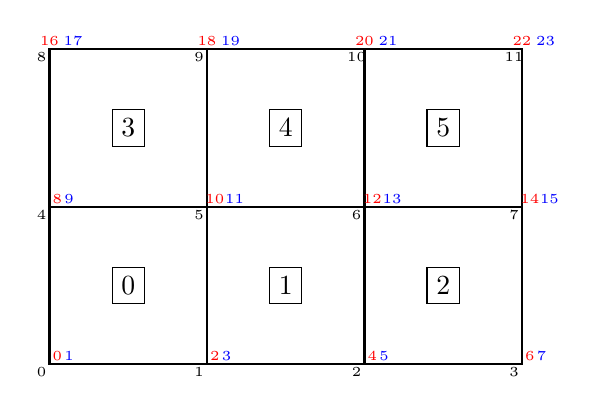
\begin{tikzpicture}
%\draw[step=0.5cm,gray,very thin] (0,0) grid (8,6); %background grid
\draw[thick] (1,1) -- (3,1) -- (3,3) -- (1,3) -- cycle;  
\draw[thick] (3,1) -- (5,1) -- (5,3) -- (3,3) -- cycle; 
\draw[thick] (5,1) -- (7,1) -- (7,3) -- (5,3) -- cycle; 
\draw[thick] (1,3) -- (3,3) -- (3,5) -- (1,5) -- cycle;  
\draw[thick] (3,3) -- (5,3) -- (5,5) -- (3,5) -- cycle; 
\draw[thick] (5,3) -- (7,3) -- (7,5) -- (5,5) -- cycle; 
\node[draw] at (2,2) {0};
\node[draw] at (4,2) {1};
\node[draw] at (6,2) {2};
\node[draw] at (2,4) {3};
\node[draw] at (4,4) {4};
\node[draw] at (6,4) {5};
%pressure dofs
\node at (0.9,0.9) {\tiny 0};
\node at (2.9,0.9) {\tiny 1};
\node at (4.9,0.9) {\tiny 2};
\node at (6.9,0.9) {\tiny 3};
\node at (0.9,2.9) {\tiny 4};
\node at (2.9,2.9) {\tiny 5};
\node at (4.9,2.9) {\tiny 6};
\node at (6.9,2.9) {\tiny 7};
\node at (0.9,4.9) {\tiny 8};
\node at (2.9,4.9) {\tiny 9};
\node at (4.9,4.9) {\tiny 10};
\node at (6.9,4.9) {\tiny 11};
%velocity dofs
\node[red] at (1.1,1.1) {\tiny 0};  \node[blue] at (1.25,1.1) {\tiny 1};
\node[red] at (3.1,1.1) {\tiny 2};  \node[blue] at (3.25,1.1) {\tiny 3};
\node[red] at (5.1,1.1) {\tiny 4};  \node[blue] at (5.25,1.1) {\tiny 5};
\node[red] at (7.1,1.1) {\tiny 6};  \node[blue] at (7.25,1.1) {\tiny 7};
\node[red] at (1.1,3.1) {\tiny 8};  \node[blue] at (1.25,3.1) {\tiny 9};
\node[red] at (3.1,3.1) {\tiny 10}; \node[blue] at (3.35,3.1) {\tiny 11};
\node[red] at (5.1,3.1) {\tiny 12}; \node[blue] at (5.35,3.1) {\tiny 13};
\node[red] at (7.1,3.1) {\tiny 14}; \node[blue] at (7.35,3.1) {\tiny 15};
\node[red] at (1.,5.1) {\tiny 16}; \node[blue] at (1.3,5.1) {\tiny 17};
\node[red] at (3.,5.1) {\tiny 18}; \node[blue] at (3.3,5.1) {\tiny 19};
\node[red] at (5.,5.1) {\tiny 20}; \node[blue] at (5.3,5.1) {\tiny 21};
\node[red] at (7.,5.1) {\tiny 22}; \node[blue] at (7.3,5.1) {\tiny 23};
\end{tikzpicture}\\
{\tiny Red color corresponds to the dofs in the x direction, blue color indicates a dof in the y direction.}
\end{center}

We have nnp=12, nel=6, NfemV=24. Let us assume that free slip boundary conditions are applied. 
The boundary conditions {\tt fix\_bc} array is then:
\begin{center}
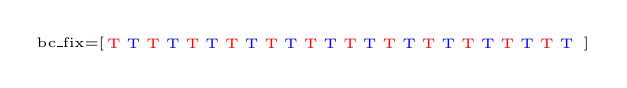
\begin{tikzpicture}
%\draw[step=0.5cm,gray,very thin] (0,0) grid (9,0.7); %background grid
\node  at (0.45,.1) {\tiny bc\_fix=[};

\node[red]  at (1.00,.1) {\tiny T};
\node[blue] at (1.25,.1) {\tiny T};
\node[red]  at (1.50,.1) {\tiny T};
\node[blue] at (1.75,.1) {\tiny T};
\node[red]  at (2.00,.1) {\tiny T};
\node[blue] at (2.25,.1) {\tiny T};
\node[red]  at (2.50,.1) {\tiny T};
\node[blue] at (2.75,.1) {\tiny T};
\node[red]  at (3.00,.1) {\tiny T};
\node[blue] at (3.25,.1) {\tiny T};
\node[red]  at (3.50,.1) {\tiny T};
\node[blue] at (3.75,.1) {\tiny T};
\node[red]  at (4.00,.1) {\tiny T};
\node[blue] at (4.25,.1) {\tiny T};
\node[red]  at (4.50,.1) {\tiny T};
\node[blue] at (4.75,.1) {\tiny T};
\node[red]  at (5.00,.1) {\tiny T};
\node[blue] at (5.25,.1) {\tiny T};
\node[red]  at (5.50,.1) {\tiny T};
\node[blue] at (5.75,.1) {\tiny T};
\node[red]  at (6.00,.1) {\tiny T};
\node[blue] at (6.25,.1) {\tiny T};
\node[red]  at (6.50,.1) {\tiny T};
\node[blue] at (6.75,.1) {\tiny T};

\node  at (7,.1) {\tiny ]};

\end{tikzpicture}\\
\end{center}
Note that since corners belong to two edges, we effectively prescribed 
no-slip boundary conditions on those. 
\todo[inline]{why does array contain only T??}


We wish to compute the tractions on the boundaries, and more precisely for the dofs for which 
a Dirichlet velocity boundary condition has been prescribed.
The number of (traction) unknowns NfemTr is then the number of {\tt T} in the {\tt bc\_fix} array.
In our specific case, we wave NfemTr= .
\todo{finish}
This means that we need for each targeted dof to be able to find its identity/number
between 0 and NfemTr-1. We therefore create the array {\tt bc\_nb} which is 
filled as follows: 
 
\begin{center}
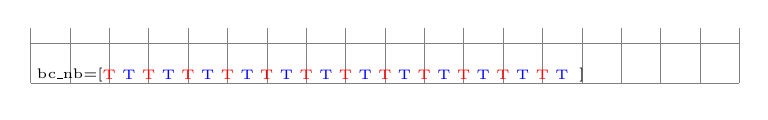
\begin{tikzpicture}
\draw[step=0.5cm,gray,very thin] (0,0) grid (9,0.7); %background grid

\node  at (0.5,.1) {\tiny bc\_nb=[};

\node[red]  at (1.00,.1) {\tiny T};
\node[blue] at (1.25,.1) {\tiny T};
\node[red]  at (1.50,.1) {\tiny T};
\node[blue] at (1.75,.1) {\tiny T};
\node[red]  at (2.00,.1) {\tiny T};
\node[blue] at (2.25,.1) {\tiny T};
\node[red]  at (2.50,.1) {\tiny T};
\node[blue] at (2.75,.1) {\tiny T};
\node[red]  at (3.00,.1) {\tiny T};
\node[blue] at (3.25,.1) {\tiny T};
\node[red]  at (3.50,.1) {\tiny T};
\node[blue] at (3.75,.1) {\tiny T};
\node[red]  at (4.00,.1) {\tiny T};
\node[blue] at (4.25,.1) {\tiny T};
\node[red]  at (4.50,.1) {\tiny T};
\node[blue] at (4.75,.1) {\tiny T};
\node[red]  at (5.00,.1) {\tiny T};
\node[blue] at (5.25,.1) {\tiny T};
\node[red]  at (5.50,.1) {\tiny T};
\node[blue] at (5.75,.1) {\tiny T};
\node[red]  at (6.00,.1) {\tiny T};
\node[blue] at (6.25,.1) {\tiny T};
\node[red]  at (6.50,.1) {\tiny T};
\node[blue] at (6.75,.1) {\tiny T};
\node  at (7,.1) {\tiny ]};
\end{tikzpicture}\\
\end{center}

This translates as follows in the code:
\begin{lstlisting}
NfemTr=np.sum(bc_fix)
bc_nb=np.zeros(NfemV,dtype=np.int32)
counter=0
for i in range(0,NfemV):
    if (bc_fix[i]):
       bc_nb[i]=counter
       counter+=1
\end{lstlisting}


The algorithm is then as follows

\begin{itemize}
\item[A] Prepare two arrays to store the matrix $M_{cbf}$ and its right hand side $rhs_{cbf}$  

\item[B] 
Loop over all elements 

\item[C] 
For each element touching a boundary, compute the residual vector 
$R_{el}=-f_{el} + \K_{el}{\cal V}_{el} + \G_{el} {\cal P}_{el}$

\item[D]
Loop over the four edges of the element using the connectivity array

\item[E]
For each edge loop over the number of degrees of freedom (2 in 2D)

\item[F] 
For each edge assess whether the dofs on both ends are target dofs. 

\item[G]
If so, compute the mass matrix $M_{edge}$ for this edge 

\item[H] extract the 2 values off the element residual vector and assemble these
in $rhs_{cbf}$

\item[I] Assemble $M_{edge}$ into NfemTrxNfemTr matrix using bc\_nb
\end{itemize}


\begin{lstlisting}
M_cbf = np.zeros((NfemTr,NfemTr),np.float64)         # A
rhs_cbf = np.zeros(NfemTr,np.float64)

for iel in range(0,nel):                             # B

    ... compute elemental residual ...               # C

    #boundary 0-1                                    # D
    for i in range(0,ndofV):                         # E
        idof0=2*icon[0,iel]+i
        idof1=2*icon[1,iel]+i
        if (bc_fix[idof0] and bc_fix[idof1]):        # F
           idofTr0=bc_nb[idof0]   
           idofTr1=bc_nb[idof1]
           rhs_cbf[idofTr0]+=res_el[0+i]             # H
           rhs_cbf[idofTr1]+=res_el[2+i]              
           M_cbf[idofTr0,idofTr0]+=M_edge[0,0]       # 
           M_cbf[idofTr0,idofTr1]+=M_edge[0,1]       # I
           M_cbf[idofTr1,idofTr0]+=M_edge[1,0]       # 
           M_cbf[idofTr1,idofTr1]+=M_edge[1,1]       #

    #boundary 1-2                                    #[D]

    ...

    #boundary 2-3                                    #[D]

    ...

    #boundary 3-0                                    #[D]

    ...


\end{lstlisting}










%---------------------------------------------------------------
\subsection{The CBF applied to the heat transport equation}

We start from the strong form of the heat transfer equation (without the source terms for simplicity):
\[
\rho C_p
\left(\frac{\partial T}{\partial t} + \vec{\upnu}\cdot \vec{\nabla}T\right)
=
\vec{\nabla} \cdot k\vec{\nabla} T
\]
The weak form then writes:
\[
\int_\Omega \bN^\uptheta
\rho C_p
\frac{\partial T}{\partial t} dV 
+
\int_\Omega \bN^\uptheta
\rho C_p
\vec{\upnu}\cdot \vec{\nabla}T  dV
=
\int_\Omega \bN^\uptheta
\vec{\nabla} \cdot k\vec{\nabla} T dV
\]
Using once again integration by parts and divergence theorem:
\[
\int_\Omega \bN^\uptheta
\rho C_p
\frac{\partial T}{\partial t} dV 
+
\int_\Omega \bN^\uptheta
\rho C_p
\vec{\upnu}\cdot \vec{\nabla}T  dV
=
\int_\Gamma \bN^\uptheta k \vec{\nabla} T \cdot \vec{n} d\Gamma
-
\int_\Omega  \vec{\nabla} \bN^\uptheta \cdot k \vec{\nabla} T dV
\]
On the boundary we are interested in the heat flux $\vec{q}=-k \vec{\nabla} T$
\[
\int_\Omega \bN^\uptheta
\rho C_p
\frac{\partial T}{\partial t} dV 
+
\int_\Omega \bN^\uptheta
\rho C_p
\vec{\upnu}\cdot \vec{\nabla} T  dV
=
-\int_\Gamma \bN^\uptheta {\bm q} \cdot {\bm n} d\Gamma
- \int_\Omega  \vec{\nabla} \bN^\uptheta \cdot k \vec{\nabla} T dV
\]
or,
\[
\int_\Gamma \bN^\uptheta {\bm q} \cdot {\bm n} d\Gamma
=
-\int_\Omega \bN^\uptheta
\rho C_p
\frac{\partial T}{\partial t} dV 
-
\int_\Omega \bN^\uptheta
\rho C_p  {\bm v}\cdot \vec{\nabla} T  dV
- \int_\Omega  \vec{\nabla} \bN^\uptheta \cdot k \vec{\nabla} T dV
\]
Considering the normal heat flux $q_n = \vec{q} \cdot \vec{n}$ as an unknown 
living on the nodes on the boundary, 
\[
q_n = \sum_{i=1}^2 q_{n|i} N_i
\]
so that the left hand term becomes a mass matrix for the basis functions living on 
the boundary.
We have already covered the right hand side terms when building the FE system 
to solve the heat transport equation, so that in the end 
\[
\M' \cdot \vec{\cal Q}_n =
- \M \cdot \frac{\partial \bm T}{\partial t} -K_a \cdot {\bm T} - K_d \cdot {\bm T} 
\]
where $\vec{\cal Q}_n$ is the assembled vector of normal heat flux components.
Note that in all terms the assembly only takes place over the elements along the boundary.


Note that the resulting matrix is symmetric.


 %-----------------------
\newpage %-----------------------------------------------------------------------------------------
\section{The value of the timestep}\label{ss:cfl} \input{cfl} %---------------------------------
\newpage %-----------------------------------------------------------------------------------------
\section{Mappings \& Jacobians \label{ss:mappings}} \begin{flushright} {\tiny {\color{gray} mappings.tex}} \end{flushright}
%~~~~~~~~~~~~~~~~~~~~~~~~~~~~~~~~~~~~~~~~~~~~~~~~~~~~~~~~~~~~~~~~~~~~~~~~~~~~~~~~~~~~~~~~~~~~~~~~~~

\index{general}{Isoparametric}
\index{general}{Subparametric} 
\index{general}{Superparametric}

The name {\sl isoparametric} derives from the fact that the same ('iso') 
functions are used as basis functions and for the mapping to the reference element.

More generally, if $n_e$ denotes the number of nodes of an element and $n_g$ denotes the 
number of nodes describing the geometry of the element, 
then the element is termed {\sl subparametric} when $n_g<n_e$ and 
{\sl superparametric} when $n_g>n_e$.

%...........................................
\subsubsection{Linear mapping on a triangle}

\begin{verbatim}
2
|\     s
| \    |_r
|  \
3===1
\end{verbatim}

Let us assume that the coordinates of the vertices are 
$(x_1,y_1)$,  
$(x_2,y_2)$, and 
$(x_3,y_3)$.
The coordinates inside the reference element are $(r,s)$ with 
$0\le r \le 1$ and $0 \le s \le 1$. We then simply have the 
following relationship, i.e. any point of the reference element 
can be mapped to the physical triangle as follows:
\begin{eqnarray}
x&=& r x_1 + s x_2 + (1-r-s) x_3 \\
y&=& r y_1 + s y_2 + (1-r-s) y_3 
\end{eqnarray} 
Note that the functions $r$, $s$ and $1-r-s$ are in fact the 
$P_1$ basis functions (see Section~\ref{ss:p1}).
There is also an inverse map, which is easily computed:
\begin{eqnarray}
r&=& \frac{(y_2-y_3)(x-x_3)-(x_2-x_3)(y-y_3)}{(x_1-x_3)(y_2-y_3)-(y_1-y_3)(x_2-x_3)} \\
s&=& \frac{-(y_1-y_3)(x-x_3)+(x_1-x_3)(y-y_3)}{(x_1-x_3)(y_2-y_3)-(y_1-y_3)(x_2-x_3)} 
\end{eqnarray} 
\begin{remark}
The denominator will not vanish, because it is a multiple of the area of the 
triangle. If the three points
are distinct then the area cannot be zero.
\end{remark}

%................................................
\subsubsection{Bilinear mapping on a quadrilateral}

The \index{general}{reference element} reference element 
is in the $(r,s)$ space. It is a square of size $2\times2$ 
centered around the origin, i.e. $(r,s)\in[-1,1]\times[-1,1]$. 
We wish to map it to the quadrilateral in the $(x,y)$ space 
(and vice versa):

\begin{center}
\includegraphics[width=8cm]{images/mappings/bilinear/mapping_bilinear.png}
\end{center}

The coordinates of the vertices are 
$(x_1,y_1)$, $(x_2,y_2)$, $(x_3,y_3)$ and $(x_4,y_4)$.
We then simply have the 
following relationship, i.e. any point of the reference element 
can be mapped to the physical quadrilateral as follows:
\begin{eqnarray}
x&=& \bN_1(r,s) x_1 + \bN_2(r,s) x_2 + \bN_3(r,s) x_3 + \bN_4(r,s) x_4 \\
y&=& \bN_1(r,s) y_1 + \bN_2(r,s) y_2 + \bN_3(r,s) y_3 + \bN_4(r,s) y_4 
\end{eqnarray} 
where the $Q_1$ basis functions $\bN_i(r,s)$ are defined in Section~\ref{sec:elts1D}.

In the following example the program randomly generates 10000 points 
inside the reference 
element and computes their mapping into the $(x,y)$ space. 

\begin{lstlisting}
x1=-1 ; y1=-2
x2=3  ; y2=-1
x3=2  ; y3=2
x4=-3 ; y4=1

npts=10000
r=np.zeros(npts,dtype=np.float64)   
s=np.zeros(npts,dtype=np.float64)   
x=np.zeros(npts,dtype=np.float64)   
y=np.zeros(npts,dtype=np.float64)   

for i in range(0,npts):
    # compute random r,s coordinates
    r[i]=random.uniform(-1.,+1)
    s[i]=random.uniform(-1.,+1)
    # compute basis function values at r,s
    N1=0.25*(1-r[i])*(1-s[i])
    N2=0.25*(1+r[i])*(1-s[i])
    N3=0.25*(1+r[i])*(1+s[i])
    N4=0.25*(1-r[i])*(1+s[i])
    # compute x,y coordinates
    x[i]=N1*x1+N2*x2+N3*x3+N4*x4
    y[i]=N1*y1+N2*y2+N3*y3+N4*y4

np.savetxt('rs.ascii',np.array([r,s]).T)
np.savetxt('xy.ascii',np.array([x,y]).T)
\end{lstlisting}

\begin{center}
\includegraphics[width=7cm]{images/mappings/bilinear/rs.pdf}
\includegraphics[width=7cm]{images/mappings/bilinear/xy.pdf}
\end{center}

There is also an inverse map, which is not so easily computed (see Section~\ref{sec:amiin}).
However, if the quadrilateral in the $(x,y)$ space is a rectangle of size $(h_x,h_y)$, 
the inverse mapping is trivial:
\begin{eqnarray}
r&=&\frac{x-x_1}{x_2-x_1} \\
s&=&\frac{y-y_1}{y_4-y_1} 
\end{eqnarray}
Also in the case of rectangular elements of size $(h_x,h_y)$
the basis functions can easily be written as functions of $(x,y)$:
\begin{eqnarray}
\bN_1(x,y) &=& \left( \frac{x_3 -x }{h_x}  \right) \left( \frac{y_3 -y }{h_y}  \right) \nn\\
\bN_2(x,y) &=& \left( \frac{x - x_1}{h_x}  \right) \left( \frac{y_3 -y }{h_y}  \right) \nn\\
\bN_3(x,y) &=& \left( \frac{x - x_1}{h_x}  \right) \left( \frac{y - y_1}{h_y}  \right) \nn\\
\bN_4(x,y) &=& \left( \frac{x_3 -x }{h_x}  \right) \left( \frac{y - y_1}{h_y}  \right) \nn 
\end{eqnarray}
On the one hand, any variable defined on the element can be approximated using the basis functions:
\begin{equation}
f^h(r,s)=\sum_i \bN_i(r,s) f_i.
\end{equation}
If we treat the coordinate variables $x$ and $y$ themselves as functions, 
then the basis functions can be used to construct the mapping:
\begin{equation}
x(r,s)=\sum_i \bN_i(r,s) x_i 
\qquad
y(r,s)=\sum_i \bN_i(r,s) y_i,  \label{eqxy}
\end{equation}
leading to write
\begin{eqnarray}
\frac{\partial x}{\partial r} &=& \sum_i \frac{\partial \bN_i}{\partial r} x_i \\
\frac{\partial x}{\partial s} &=& \sum_i \frac{\partial \bN_i}{\partial s} x_i \\
\frac{\partial y}{\partial r} &=& \sum_i \frac{\partial \bN_i}{\partial r} y_i \\
\frac{\partial y}{\partial s} &=& \sum_i \frac{\partial \bN_i}{\partial s} y_i 
\end{eqnarray}
On the other hand we also have 
\begin{eqnarray}
\frac{\partial f}{\partial r} &=&
\frac{\partial f}{\partial x}\frac{\partial x}{\partial r}
+\frac{\partial f}{\partial y}\frac{\partial y}{\partial r} \\
\frac{\partial f}{\partial s} &=&
\frac{\partial f}{\partial x}\frac{\partial x}{\partial s}
+\frac{\partial f}{\partial y}\frac{\partial y}{\partial s}
\end{eqnarray}
or in matrix form:
\begin{equation}
\left(
\begin{array}{c}
\frac{\partial f}{\partial r} \\ \\
\frac{\partial f}{\partial s}
\end{array}
\right)
=
\underbrace{
\left(
\begin{array}{cc}
\frac{\partial x}{\partial r} & \frac{\partial y}{\partial r} \nonumber\\ \\
\frac{\partial x}{\partial s} & \frac{\partial y}{\partial s} \nonumber
\end{array}
\right)
}_{\bm J}
\cdot
\left(
\begin{array}{c}
\frac{\partial f}{\partial x} \\ \\
\frac{\partial f}{\partial y}
\end{array}
\right)
\end{equation}
where ${\bm J}$ is called the Jacobian of the transformation
By inverting the Jacobian matrix, the desired derivatives with respect to $x$
and $y$ can be obtained:

We have:
\[
\left(
\begin{array}{c}
\frac{\partial f}{\partial x} \\ \\
\frac{\partial f}{\partial y}
\end{array}
\right)
=
{\bm J}^{-1} \cdot 
\left(
\begin{array}{c}
\frac{\partial f}{\partial r} \\ \\
\frac{\partial f}{\partial s}
\end{array}
\right)
\]
The inverse of the Jacobian matrix can be simply obtained in 
2D (Cramer's rule for $2\times2$ matrices\footnote{\url{https://en.wikipedia.org/wiki/Cramers_rule}}):
\[
{\bm J}^{-1} = \frac{1}{|{\bm J}|} 
\left(
\begin{array}{cc}
\frac{\partial y}{\partial s} & -\frac{\partial y}{\partial r} \nonumber\\ \\
-\frac{\partial x}{\partial s} & \frac{\partial x}{\partial r} \nonumber
\end{array}
\right)
\]
The presence of the determinant in the denominator implies that it cannot 
be zero anywhere, or in other words: the mapping is not valid if $|{\bm J}|$
is zero anywhere over the element.

\begin{remark}
\textcite{hua90} (1990) has published analytical inverse transformation 
for quadrilateral isoparametric elements, i.e. how to compute ${\bm J}^{-1}$ 
as a function of space coordinates and not just at the quadrature points. 
\end{remark}

Let us look at this by means of a simple example and let us consider the following 
element:
\begin{center}
\includegraphics[width=4cm]{images/mappings/fournode/ex1}
\end{center}
Then a $Q_1$ mapping yields:
\begin{eqnarray}
x(r,s) &=& \sum_i \bN_i(r,s) x_i = \bN_2 + 2\bN_3 = \frac{1}{4} (3+3r+ s+rt) \nn\\
y(r,s) &=& \sum_i \bN_i(r,s) y_i = 2\bN_3 + \bN_4 = \frac{1}{4} (3+r+ 3s+rt) 
\end{eqnarray}
The Jacobian matrix is then
\begin{equation}
{\bm J} = 
\left(
\begin{array}{cc}
\frac{\partial x}{\partial r} & \frac{\partial y}{\partial r} \nonumber\\ \\
\frac{\partial x}{\partial s} & \frac{\partial y}{\partial s} \nonumber
\end{array}
\right)
=
\frac{1}{4}
\left(
\begin{array}{cc}
3+s & 1+s \\
1+r & 3+r
\end{array}
\right)
\end{equation}
and its determinant is 
\begin{equation}
|{\bm J}|=\frac{1}{4} [(3+s)(3+r)-(1+s)(1+r)]=\frac{1}{2}+\frac{1}{8}r+\frac{1}{8}s
\end{equation}
It is clear that $|{\bm J}|>0$ for $-1\leq r \leq +1$ and $-1\leq s \leq +1$. 

Let us now consider another example, the following element:
\begin{center}
\includegraphics[width=3.5cm]{images/mappings/fournode/ex2}
\end{center}
It follows that
\begin{eqnarray}
x(r,s) &=& \sum_i \bN_i(r,s) x_i = \frac{1}{4}(1+r)(7+5s) \\ 
y(r,s) &=& \sum_i \bN_i(r,s) y_i = \frac{1}{4}(17+5r+7s-5rs)
\end{eqnarray}
and the determinant:
\[
|{\bm J}|=\frac{3}{2}-\frac{15r}{4}+\frac{15s}{4}
\]
is zero for $r-s=2/5$. This mapping is invalid!

\begin{remark}
Problems also arise when the Jacobian matrix is nearly singular due to round-off errors.
To avoid problems linked to badly shaped elements, it is recommended that the inside
angles of an element are larger than $15\degree$ and less than $165\degree$.
\end{remark}

From Eq.~\eqref{eqxy}, we can also write:
\begin{eqnarray}
dx &=& \frac{\partial x}{\partial r} dr + \frac{\partial x}{\partial s} ds \\
dy &=& \frac{\partial y}{\partial r} dr + \frac{\partial y}{\partial s} ds 
\end{eqnarray}
or, 
\begin{equation}
\left(
\begin{array}{c}
dx \\ dy
\end{array}
\right)
={\bm J}\cdot
\left(
\begin{array}{c}
dr \\ ds
\end{array}
\right)
\end{equation}
This means that integrating over the 'real' element in $(x,y)$ space
can be simply done by integrating of the reference element in the 
$(r,s)$ space. This is the cornerstone of most of the implementation of the 
Finite Element Method, the second integral being carried out by means 
of the Gauss-Legendre quadrature.

\begin{equation}
\iint_{\Omega_e} ... \; dx dy = \int_{-1}^{+1} \int_{-1}^{+1} ...|{\bm J}| \; dr ds
\end{equation}


%.................................................................
\subsubsection{Biquadratic mapping of a straight-edge face $Q_2$ element }

\begin{center}
\includegraphics[width=8cm]{images/mappings/biquadratic/mapping1}
\end{center}

The reference element now contains 9 nodes: 1,3,7,9 are the corners, nodes
2,4,6,8 are the mid-face points and node 5 is in the middle\footnote{Note that 
this numbering is quite arbitrary}.
The mapping from the $(r,s)$ space to the $(x,y)$ space is then as follows:

\begin{eqnarray}
\left(
\begin{array}{c}
x(r,s) \\ y(r,s)
\end{array}
\right)
&=&
\bN_1(r,s)
\left(
\begin{array}{c}
x_1 \\ y_1
\end{array}
\right)
+
\bN_2(r,s)
\left(
\begin{array}{c}
x_2 \\ y_2
\end{array}
\right)
+
\bN_3(r,s)
\left(
\begin{array}{c}
x_3 \\ y_3
\end{array}
\right)
+
\bN_4(r,s)
\left(
\begin{array}{c}
x_4 \\ y_4
\end{array}
\right) \nonumber\\
&+&
\bN_5(r,s)
\left(
\begin{array}{c}
x_5 \\ y_5
\end{array}
\right)
+
\bN_6(r,s)
\left(
\begin{array}{c}
x_6 \\ y_6
\end{array}
\right)
+
\bN_7(r,s)
\left(
\begin{array}{c}
x_7 \\ y_7
\end{array}
\right)
+
\bN_8(r,s)
\left(
\begin{array}{c}
x_4 \\ y_8
\end{array}
\right) \nonumber\\
&+&
\bN_9(r,s)
\left(
\begin{array}{c}
x_9 \\ y_9
\end{array}
\right) 
\nonumber
\end{eqnarray}
where the $Q_2$ basis functions have been obtained in Section~\ref{ss:q22d}:
\begin{eqnarray}
\bN_1(r,t)&=& 0.5r(r-1)  0.5t(t-1) \nonumber\\
\bN_2(r,t)&=&      (1-r^2)  0.5t(t-1) \nonumber\\
\bN_3(r,t)&=& 0.5r(r+1)  0.5t(t-1) \nonumber\\
\bN_4(r,t)&=& 0.5r(r-1)       (1-t^2) \nonumber\\
\bN_5(r,t)&=&      (1-r^2)       (1-t^2) \nonumber\\
\bN_6(r,t)&=& 0.5r(r+1)       (1-t^2) \nonumber\\
\bN_7(r,t)&=& 0.5r(r-1)  0.5t(t+1) \nonumber\\
\bN_8(r,t)&=&      (1-r^2)  0.5t(t+1) \nonumber\\
\bN_9(r,t)&=& 0.5r(r+1)  0.5t(t+1) \nonumber
\end{eqnarray}


\begin{lstlisting}
x1=-1                 ; y1=-2
x3=3                  ; y3=-1
x9=2                  ; y9=2
x7=-3                 ; y7=1
x2=0.5*(x1+x3)        ; y2=0.5*(y1+y3)
x4=0.5*(x1+x7)        ; y4=0.5*(y1+y7)
x6=0.5*(x3+x9)        ; y6=0.5*(y3+y9)
x8=0.5*(x7+x9)        ; y8=0.5*(y7+y9)
x5=0.25*(x1+x3+x7+x9) ; y5=0.25*(y1+y3+y7+y9)

npts=10000
r=np.zeros(npts,dtype=np.float64)   
s=np.zeros(npts,dtype=np.float64)   
xQ1=np.zeros(npts,dtype=np.float64)   
yQ1=np.zeros(npts,dtype=np.float64)   
xQ2=np.zeros(npts,dtype=np.float64)   
yQ2=np.zeros(npts,dtype=np.float64)   

for i in range(0,npts):
    # compute random r,s coordinates
    r[i]=random.uniform(-1.,+1)
    s[i]=random.uniform(-1.,+1)
    # compute Q2 basis function values at r,s
    N1= 0.5*r[i]*(r[i]-1.) * 0.5*s[i]*(s[i]-1.)
    N2=       (1.-r[i]**2) * 0.5*s[i]*(s[i]-1.)
    N3= 0.5*r[i]*(r[i]+1.) * 0.5*s[i]*(s[i]-1.)
    N4= 0.5*r[i]*(r[i]-1.) *       (1.-s[i]**2)
    N5=       (1.-r[i]**2) *       (1.-s[i]**2)
    N6= 0.5*r[i]*(r[i]+1.) *       (1.-s[i]**2)
    N7= 0.5*r[i]*(r[i]-1.) * 0.5*s[i]*(s[i]+1.)
    N8=       (1.-r[i]**2) * 0.5*s[i]*(s[i]+1.)
    N9= 0.5*r[i]*(r[i]+1.) * 0.5*s[i]*(s[i]+1.)
    # compute x,y coordinates
    xQ2[i]=N1*x1+N2*x2+N3*x3+N4*x4+N5*x5+N6*x6+N7*x7+N8*x8+N9*x9
    yQ2[i]=N1*y1+N2*y2+N3*y3+N4*y4+N5*y5+N6*y6+N7*y7+N8*y8+N9*y9
    # compute Q1 basis function values at r,s
    N1=0.25*(1-r[i])*(1-s[i])
    N2=0.25*(1+r[i])*(1-s[i])
    N3=0.25*(1+r[i])*(1+s[i])
    N4=0.25*(1-r[i])*(1+s[i])
    # compute x,y coordinates
    xQ1[i]=N1*x1+N2*x3+N3*x9+N4*x7
    yQ1[i]=N1*y1+N2*y3+N3*y9+N4*y7

np.savetxt('rs.ascii',np.array([r,s]).T)
np.savetxt('xyQ1.ascii',np.array([xQ1,yQ1]).T)
np.savetxt('xyQ2.ascii',np.array([xQ2,yQ2]).T)
\end{lstlisting}

The code is available in {\tt /images/mappings/biquadratic}
Note that the coordinates of point 5 are defined being those of the barycenter
of the quadrilateral. More on this choice later.

\begin{center}
a)\includegraphics[width=5.6cm]{images/mappings/biquadratic/rs.pdf}
b)\includegraphics[width=5.6cm]{images/mappings/biquadratic/xyQ1.pdf}
c)\includegraphics[width=5.6cm]{images/mappings/biquadratic/xyQ2.pdf}\\
{\captionfont a) 10,000 random points in the reference element; 
b,c) image of these points by means of a bilinear and biquadratic mapping 
respectively.\\ When the sides of the element
are straight we see that a $Q_1$ mapping is sufficient.}
\end{center}

%.................................................................
\subsubsection{Biquadratic mapping of a not-so straight-line face $Q_2$ element }

We now carry out the same exercise as before but nodes 2 and 8 are no more 
in the middle of nodes 1-3 and 7-9 respectively.
The code is available in {\tt /images/mappings/biquadratic2}.

\begin{center}
a)\includegraphics[width=4.5cm]{images/mappings/biquadratic2/rs.pdf}
b)\includegraphics[width=4.5cm]{images/mappings/biquadratic2/xyQ1.pdf}
c)\includegraphics[width=4.5cm]{images/mappings/biquadratic2/xyQ2.pdf}\\
{\captionfont a) 10,000 random points in the reference element; 
b,c) image of these points by means of a bilinear and biquadratic mapping 
respectively.} 
\end{center}

In this case we see that 
the $Q_2$ mapping manages to better capture the 'real' shape of the element.
Since nodes 2 and 8 have moved, we could now ask ourselves 
where we should place node 5? In this example we set it as follows
but it is somewhat arbitrary.
\begin{lstlisting}
x5=(x1+x2+x3+x4+x6+x7+x8+x9)/8. 
y5=(y1+y2+y3+y4+y6+y7+y8+y9)/8.
\end{lstlisting}
We will come back to this later.

%.......................................................................
\subsubsection{Bilinear, biquadratic and bicubic mapping in an annulus }

In the light of what precedes, we can now ask ourselves how this translates to 
a real geodynamic case. Let us then consider the case of an annular domain, 
a cross section of a hollow sphere. 
When using quadrilateral elements, the mesh will look similar to this:

\begin{center}
\includegraphics[width=6cm]{images/mappings/curved/annulus_mesh}
\end{center}

We here focus on $Q_1$, $Q_2$ and $Q_3$ mappings. We single out an element, 
and arbitrarily define it as follows in polar coordinates:
\begin{lstlisting}
theta1=23./180.*np.pi
theta2=52./180.*np.pi
R1=1.
R2=1.5
\end{lstlisting}
The $Q_1$ mapping requires four points, the $Q_2$ nine points and the $Q_3$
sixteen points. 
The code used in the following is available at {\tt ./images/mappings/curved/}.
These are placed equidistantly in the $r,\theta$ coordinate
system, as shown hereunder:

\begin{center}
\includegraphics[width=5.7cm]{images/mappings/curved/nodesQ1.pdf}
\includegraphics[width=5.7cm]{images/mappings/curved/nodesQ2.pdf}
\includegraphics[width=5.7cm]{images/mappings/curved/nodesQ3.pdf}\\
{\captionfont Left to right: position of the nodes for the $Q_1$, $Q_2$ and $Q_3$ mappings.
$Q_4$ is not shown.}
\end{center}

As before, we randomly shoot 10,000 points inside the reference element 
and map these out in the $x,y$ space. Resulting swarms of points are shown 
in the following figures:

\begin{center}
\includegraphics[width=5.7cm]{images/mappings/curved/xy1_keep.pdf}
\includegraphics[width=5.7cm]{images/mappings/curved/xy2_keep.pdf}
\includegraphics[width=5.7cm]{images/mappings/curved/xy3_keep.pdf}\\
{\captionfont Left to right: position of the mapped points for the $Q_1$, $Q_2$ and $Q_3$ mappings.
$Q_4$ is not shown.}
\end{center}

The image of a square with a $Q_1$ mapping is obviously a quadrilateral
so that it looks like quite a few points land outside of the domain $R_1\leq r\leq R_2$.
Note that points are well within $23\degree \leq \theta \leq 52\degree$, which can 
simply be explained by the fact that the faces of the element joining $R_1$
to $R_2$ are straight lines.

However, it looks like the biquadratic and bicubic mappings are doing a much better 
job at mapping the region of space $R_1\leq r\leq R_2$. In order to characterise 
this better, we now place 10,000 points on the bottom face of 
the reference element (i.e. $s=-1$)
and once again compute their coordinates in the the $x,y$ space:

\begin{center}
\includegraphics[width=8cm]{images/mappings/curved/xy1.pdf}
\includegraphics[width=8cm]{images/mappings/curved/xy2.pdf}\\
\includegraphics[width=8cm]{images/mappings/curved/xy3.pdf}
\includegraphics[width=8cm]{images/mappings/curved/xy4.pdf}\\
{\captionfont Position of the mapped points for the $Q_1$, $Q_2$, $Q_3$ and $Q_4$ mappings.}
\end{center}

For each point $i$ we now compute the distance $r_i$ 
to the origin, which, if the 
mapping was perfect, would be exactly equal to $R_1=1$. 
On the following plots are shown the error $r_i-1$ for all 
points, from $r=-1$ to $r=+1$.

\begin{center}
\includegraphics[width=8cm]{images/mappings/curved/innerline_error_Q1mapping.pdf}
\includegraphics[width=8cm]{images/mappings/curved/innerline_error_Q2mapping.pdf}\\
\includegraphics[width=8cm]{images/mappings/curved/innerline_error_Q3mapping.pdf}
\includegraphics[width=8cm]{images/mappings/curved/innerline_error_Q4mapping.pdf}\\
{\captionfont Radius error of the mapped points for the $Q_1$, $Q_2$, $Q_3$ and $Q_4$ mappings.}
\end{center}

We see that the amplitude of the error decreases with the order of the mapping used, 
which is why for instance \aspect uses a $Q_4$ mapping by default\footnote{I find it also quite striking 
that the $Q_4$ mapping outperforms the $Q_3$ one by two orders of magnitude...}.
Actually, in this particular case, the equation which describes the circle is not a 
polynomial so that no high-order mapping will ever be able to {\it exactly} 
represent the curved boundary of the element!

Another interesting point to keep in mind is that the location of the quadrature points
in the $x,y$ space is also determined by the mapping used, which can have consequences
on the accuracy of the integration and it will be reflected (for instance) on the 
error convergence rate.

As already mentioned previously, 
the coordinates of the nodes of the element in the $x,y$ are 
uniquely determined when they are on the convex hull of the element (
for instance nodes 0-7 for $Q_2$) but we need to choose the position 
of the last nodes which are inside the element. Unfortunately, this choice is 
not neutral. 

Finally, we can explore the importance of the mapping in combination with 
numerical quadrature. For each mapping we compute the area of the element
by means of a 3x3, 4x4 or 5x5 quadrature.

\begin{verbatim}
**********Q1*********
nqperdim= 3 0.3030060126539606 rel. error -0.04215361698430029
nqperdim= 4 0.3030060126539606 rel. error -0.04215361698430012 ~ 4%
nqperdim= 5 0.3030060126539606 rel. error -0.04215361698430012
**********Q2*********
nqperdim= 3 0.3162980025394154 rel. error -0.00013569026611326453
nqperdim= 4 0.3162980025394155 rel. error -0.00013569026611308905 ~ 0.01%
nqperdim= 5 0.3162980025394154 rel. error -0.00013569026611326453
**********Q3*********
nqperdim= 3 0.3163472223929359 rel. error 1.9900899402587318e-05
nqperdim= 4 0.316347222392936  rel. error 1.9900899402938278e-05 ~ 0.002%
nqperdim= 5 0.316347222392936  rel. error 1.9900899402938278e-05
**********Q4*********
nqperdim= 3 0.3163409410866220 rel. error 4.477021014282521e-08
nqperdim= 4 0.3163409541901677 rel. error 8.619243716974044e-08 ~ 0.000008%
nqperdim= 5 0.316340954190168  rel. error 8.619243804713484e-08
\end{verbatim}

Here again the $Q_4$ mapping makes quite the difference. 

\newpage

%..................................................................
\subsubsection{Biquadratic mapping - the middle node conundrum}

Python code at {\tt images/mappings/biquadratic3}.

As mentioned before, unless the element is a straight-edge quadrilateral, 
determining the (best) position of the middle node is not trivial. Or is it?


\begin{verbatim}

4--7--3
|     |
8  9  6   (reference element)
|     |
1--5--2

\end{verbatim}

We will here consider 5 different elements:

\begin{center}
\includegraphics[width=3.5cm]{images/mappings/biquadratic3/elt0/element0}
\includegraphics[width=3.5cm]{images/mappings/biquadratic3/elt1/element1}
\includegraphics[width=3.5cm]{images/mappings/biquadratic3/elt2/element2}
\includegraphics[width=3.5cm]{images/mappings/biquadratic3/elt3/element3}
\includegraphics[width=3.5cm]{images/mappings/biquadratic3/elt4/element4}\\
{\captionfont From left to right: element 0,1,2,3,4.}
\end{center}

We can think of multiple ways to come up with the 'center' of the element, 
i.e. the location of point I.

\begin{itemize}
\item {\python center=0}: 
\[
x_9=(x_1+x_2+x_3+x_4)/4 
\qquad
y_9=(y_1+y_2+y_3+y_4)/4
\]

\item {\python center=1}: 
\[
x_9=(x_1+x_2+x_3+x_4+x_5+x_6+x_7+x_8)/8 
\qquad
y_9=(y_1+y_2+y_3+y_4+y_5+y_6+y_7+y_8)/8
\]
\item {\python center=2}:
\[
x_9=(x_1+x_2+x_3+x_4+3x_5+3x_6+3x_7+3x_8)/16. 
\qquad
y_9=(y_1+y_2+y_3+y_4+3y_5+3y_6+3y_7+3y_8)/16.
\]
\item {\python center=3}: (only element=4)
\[
x_9=\frac12(R_1+R_2)\cos(3\pi/8) 
\qquad
y_9=\frac12(R_1+R_2)\sin(3\pi/8)
\]
\item {\python center=4}: I is the center of mass. 
The element is defined by $R_1<r<R_2$ and $\theta_1<\theta<\theta_2$.

We need to compute\footnote{\url{https://en.wikipedia.org/wiki/Center_of_mass}}
\begin{eqnarray}
\vec{R} 
&=&\frac{1}{M} \int \vec{r} \rho(\vec r) dV \nn\\
&=&\frac{1}{M} \rho_0 \int \vec{r} dV\nn\\
&=&\frac{1}{M} \frac{M}{V} \int \vec{r} dV\nn\\
&=&\frac{1}{V} \int \vec{r} dV\nn\\
&=&\frac{1}{V} \int \left(\begin{array}{c} x \\ y \end{array}\right)  dV\nn\\
&=&\frac{1}{V} \int \left(\begin{array}{c} r \cos \theta \\ r \sin\theta \end{array}\right)dV\nn\\
&=&\frac{1}{V} \int_{R_1}^{R_2} \int_{\theta_1}^{\theta_2} \left(\begin{array}{c} r \cos \theta 
\\ r \sin\theta \end{array}\right)  r dr d\theta\nn\\
&=&\frac{1}{\frac12 (R_2^2-R_1^2) (\theta_2-\theta_1)} \frac13(R_2^3-R_1^3) 
\left(
\begin{array}{c}
\sin\theta_2-\sin\theta_1 \\
-\cos\theta_2+\cos\theta_1 
\end{array}
\right) \nn\\
&\simeq& 
\left(
\begin{array}{c}
0.5801028000103104\\
1.4004920473554983
\end{array}
\right) 
\end{eqnarray}
which corresponds to $r=1.5158816686291174$ and $\theta=67.5^o=3\pi/8$.

\item {\python center=5}: variable position
\end{itemize}


isoparametric mapping. 


At each point $(r,s)$ we compute the error $|\sum_i N_i(r,s) x_i^2 - (\sum_i N_i(r,s) x_i)^2|$.

position of edges (setting r=+- 1, s=+-1) independent of position of middle node since shape functions are zero there

area indep of position middle node ?



%....................
\paragraph{Element 0}

In this case all only {\python center=0,1,2,4} are applicable but they all 
lead to the same point I with $x_I=0,y_I=0$. This means that the position of 
quadrature points is also independent of the {\python center} parameter.
 
\begin{center}
\includegraphics[width=5.7cm]{images/mappings/biquadratic3/elt0/jcob}
\includegraphics[width=5.7cm]{images/mappings/biquadratic3/elt0/error_posx2}
\includegraphics[width=5.7cm]{images/mappings/biquadratic3/elt0/error_posy2}\\
{\captionfont 10,000 points at random.} 
\end{center}

%....................
\paragraph{Element 1}

In this case all only {\python center=0,1,2,4} are applicable but they all 
lead to the same point I with $x_I=0,y_I=0$. This means that the position of 
quadrature points is also independent of the {\python center} parameter.
 
\begin{center}
\includegraphics[width=5.7cm]{images/mappings/biquadratic3/elt1/jcob}
\includegraphics[width=5.7cm]{images/mappings/biquadratic3/elt1/error_posx2}
\includegraphics[width=5.7cm]{images/mappings/biquadratic3/elt1/error_posy2}\\
{\captionfont 10,000 points at random.} 
\end{center}


%....................
\paragraph{Element 2} .

\begin{center}
\includegraphics[width=5.7cm]{images/mappings/biquadratic3/elt2/jcob_0}
\includegraphics[width=5.7cm]{images/mappings/biquadratic3/elt2/jcob_1}
\includegraphics[width=5.7cm]{images/mappings/biquadratic3/elt2/jcob_2}\\
\includegraphics[width=5.7cm]{images/mappings/biquadratic3/elt2/error_posx2_0}
\includegraphics[width=5.7cm]{images/mappings/biquadratic3/elt2/error_posx2_1}
\includegraphics[width=5.7cm]{images/mappings/biquadratic3/elt2/error_posx2_2}\\
\includegraphics[width=5.7cm]{images/mappings/biquadratic3/elt2/error_posy2_0}
\includegraphics[width=5.7cm]{images/mappings/biquadratic3/elt2/error_posy2_1}
\includegraphics[width=5.7cm]{images/mappings/biquadratic3/elt2/error_posy2_2}\\
{\captionfont 50,000 points at random. From left to right: center=0,1,2.} 
\end{center}




%....................
\paragraph{Element 3} .

\begin{center}
\includegraphics[width=5.7cm]{images/mappings/biquadratic3/elt3/jcob_0}
\includegraphics[width=5.7cm]{images/mappings/biquadratic3/elt3/jcob_1}
\includegraphics[width=5.7cm]{images/mappings/biquadratic3/elt3/jcob_2}\\
{\captionfont 50,000 points at random. From left to right: center=0,1,2.} 
\end{center}




%....................
\paragraph{Element 4}


\begin{center}
\includegraphics[width=5.7cm]{images/mappings/biquadratic3/elt4/jcob_0}
\includegraphics[width=5.7cm]{images/mappings/biquadratic3/elt4/jcob_1}
\includegraphics[width=5.7cm]{images/mappings/biquadratic3/elt4/jcob_2}\\
\includegraphics[width=5.7cm]{images/mappings/biquadratic3/elt4/jcob_3}
\includegraphics[width=5.7cm]{images/mappings/biquadratic3/elt4/jcob_4}\\
{\captionfont 50,000 points at random. From left to right: center=0,1,2,3,4.} 
\end{center}




\begin{center}
\includegraphics[width=8.5cm]{images/mappings/biquadratic3/elt4/nodes}
\includegraphics[width=8.5cm]{images/mappings/biquadratic3/elt4/quads}\\
{\captionfont Left: position of the nodes. Right position of quadrature points with 
nqperdim=3.}
\end{center}

\begin{verbatim}

\end{verbatim}

Area does not depend on position of middle node?!




\vspace{1cm}

\Literature 
\begin{itemize}
\item \fullcite{yuhy94}
\end{itemize}








 
 %--------------------------
\newpage %-----------------------------------------------------------------------------------------
\section{Exporting data to vtk/vtu format} 
This format seems to be the universally accepted format for 2D and 3D visualisation in 
Computational Geodynamics (and even CFD ?). Such files can be opened with open source 
softwares such as 
Paraview \footnote{https://www.paraview.org/}, 
MayaVi \footnote{https://docs.enthought.com/mayavi/mayavi/}
or Visit \footnote{https://wci.llnl.gov/simulation/computer-codes/visit/}.

Unfortunately it is my experience that no simple tutorial exists about how to build 
such files. There is an official document which describes the vtk 
format\footnote{https://www.vtk.org/wp-content/uploads/2015/04/file-formats.pdf}
but it delivers the information in a convoluted way. I therefore describe hereafter 
how fieldstone builds the vtk files. 

I hereunder show vtk file corresponding to a 3x2 grid made of linear elements.
In this particular example there are:
\begin{itemize}
\item 12 nodes and 6 elements
\item 1 elemental field (the pressure {\tt p}
\item 2 nodal fields: 1 scalar (the smoothed pressure {\tt q}), 1 vector (the velocity field {\tt u,v,0})
\end{itemize}
Note that vtk files are inherently 3D so that even in the case of a 2D simulation the $z$-coordinate 
of the points and for instance their $z$-velocity component must be provided.
The file, usually called {\filenamefont solution.vtk} starts with a header:

\lstinputlisting[language=python,firstline=1,lastline=3]{images/vtk/solution.vtu}

We then proceed to write the node coordinates as follows:

\lstinputlisting[language=python,firstline=4,lastline=19]{images/vtk/solution.vtu}

These are followed by the elemental field(s):

\lstinputlisting[language=python,firstline=20,lastline=29]{images/vtk/solution.vtu}

Nodal quantities are written next:

\lstinputlisting[language=python,firstline=30,lastline=59]{images/vtk/solution.vtu}

To these informations we must append 3 more datasets. The first one is the connectivity, 
the second one is the offsets and the third one is the type. The first one is trivial
since the required connectivity array is the same as the one needed for the Finite Elements. 
The second must be understood as follows:
when reading the connectivity information in a linear manner the offset values 
indicate the beginning of each element (omitting the zero value). The third is simply the type of element 
as given in the vtk format document (9 corresponds to a generic quadrilateral with an 
internal numbering consistent with ours). 

\lstinputlisting[language=python,firstline=60,lastline=85]{images/vtk/solution.vtu}

The file is then closed with

\lstinputlisting[language=python,firstline=86,lastline=88]{images/vtk/solution.vtu}

The {\sl solution.vtu}\footnote{\url{https://raw.githubusercontent.com/cedrict/fieldstone/master/images/vtk/solution.vtu}}  
can then be opened with ParaView, MayaVi or Visit and the reader 
is advised to find tutorials online on how to install and use these softwares. Also check Appendix~\ref{app:paraview}.

\begin{center}
\includegraphics[width=4cm]{images/vtk/grid}
\includegraphics[width=4cm]{images/vtk/vel}
\includegraphics[width=4cm]{images/vtk/press}
\end{center}

In the same folder {\tt images/vtk} there is the python script 
{\pythonfile makevtu.py}\footnote{\url{https://raw.githubusercontent.com/cedrict/fieldstone/master/images/vtk/makevtu.py}} which produces 3 different vtu files. The first one {\sl solution1.vtu} is a similar to the one above: an \lstinline{nelx*nely} quadrilateral-based mesh in a unit square. 
The second one ({\sl solution2.vtu}) looks identical when opened in Paraview but it is rather different: each element is exported as its own sub-mesh, so that if the mesh counts nel elements the number of vertices is \lstinline{4*nel}, and not \lstinline{(nelx+1)(nely+1)}. As such this file is larger. The icon array is needed to write down the positions of the four vertices of each element but not to write down the connectivity since the first 4 points are making the 1st element, the next four points are making the second element, etc ...

\begin{lstlisting}
vtufile.write("<Points> \n")
vtufile.write("<DataArray type='Float32' NumberOfComponents='3' Format='ascii'> \n")
for iel in range(0,nel):
    if not flag[iel]:
       for k in range(0,m):
           vtufile.write("%10e %10e %10e \n" %(x[icon[k,iel]],y[icon[k,iel]],0.))
vtufile.write("</DataArray>\n")
vtufile.write("</Points> \n")
vtufile.write("<Cells>\n")
vtufile.write("<DataArray type='Int32' Name='connectivity' Format='ascii'> \n")
for iel in range (0,nel_left):
    vtufile.write("%d %d %d %d \n" %(iel*4,iel*4+1,iel*4+2,iel*4+3))
vtufile.write("</DataArray>\n")
...
vtufile.write("</Cells>\n")
\end{lstlisting}

This format is rather practical in the case of linear or higher order discontinuous fields. For example, in the case of the $Q_2\times P_{-1}$ element pair, the pressure is linear inside each element and discontinuous across element edges. One can then assign pressure values at the four vertices of each element.

Finally a third mesh {\sl solution3.vtu} is produced. It is based on the 2nd one, but since elements are now somewhat de-coupled, then one can export only a subset of the mesh. For instance one could not show elements which are two distorted, or below a certain line, or outside a certain volume, etc ... In {\pythonfile makevtu.py} all elements which center is inside a circle are flagged and will not be exported into the vtu file:
\begin{lstlisting}
for iel in range(0,nel):
    flag[iel]= (xc[iel]-0.333*Lx)**2+(yc[iel]-0.666*Ly)**2<0.234**2
nel_flagged=np.sum(flag)
nel_left=nel-nel_flagged
\end{lstlisting}

\begin{center}
\includegraphics[width=11cm]{images/vtk/mesh3}
\end{center}





 %---------------------------
\newpage %-----------------------------------------------------------------------------------------
\section{Runge-Kutta methods}\label{ss:rkm} These methods were developed around 1900 by the German mathematicians Carl Runge and Martin Kutta.
The RK methods are methods for the numerical integration of 
ODEs\footnote{\url{https://en.wikipedia.org/wiki/Runge-Kutta_methods}}. These methods are well 
documented in any numerical analysis textbook and the reader is referred to \cite{gery10,tack10}.
Any Runge-Kutta method is uniquely identified by its Butcher tableau (REF?) which contains 
all necessary coefficients to build the algorithm.\todo{missing refs for Butcher tableau}

You will find here\footnote{\url{https://en.wikipedia.org/wiki/List_of_Runge-Kutta_methods}}
a complete list of RK methods.

The simplest Runge-Kutta method is the (forward) Euler method. Its tableau is:

\begin{mdframed}[backgroundcolor=blue!5]
\begin{tabular}{c|c}
0 & \\
\hline
 & 1
\end{tabular}
\end{mdframed}

\index{general}{Midpoint Method} \index{general}{RK2}
The standard second-order RK method method (also called midpoint method) is:

\begin{mdframed}[backgroundcolor=blue!5]
\begin{tabular}{c|cccccc}
0 & \\
1/2 & 1/2 \\
\hline
 & 0 & 1 
\end{tabular}
\end{mdframed}

\index{general}{Heun's emthod}
Another second-order RK method, called Heun's 
method\footnote{\url{https://en.wikipedia.org/wiki/Heun's_method}} is follows:

\begin{mdframed}[backgroundcolor=blue!5]
\begin{tabular}{c|cccccc}
0 & \\
1 & 1 \\
\hline
 & 1/2 & 1/2 
\end{tabular}
\end{mdframed}

A third-order RK method is as follows:\index{general}{RK3}

\begin{mdframed}[backgroundcolor=blue!5]
\begin{tabular}{c|ccccc}
0 & \\
1/2 & 1/2 \\
1 & -1 & 2 \\ 
\hline
 & 1/6 & 4/6  & 1/6
\end{tabular}
\end{mdframed}


\index{general}{RK4}
The RK4 method falls in this framework. Its tableau is:

\begin{mdframed}[backgroundcolor=blue!5]
\begin{tabular}{c|cccccc}
0 & \\
1/2 & 1/2 \\
1/2 & 0 & 1/2 \\
1 & 0 & 0 & 1 \\
\hline
 & 1/6 & 1/3 & 1/3 & 1/6 
\end{tabular}
\end{mdframed}

A slight variation of the standard RK4 method is also due to Kutta in 1901 and is called the 3/8-rule. 
Almost all of the error coefficients are smaller than in the standard method but it requires 
slightly more FLOPs per time step. Its Butcher tableau is

\begin{mdframed}[backgroundcolor=blue!5]
\begin{tabular}{c|cccccc}
0 & \\
1/3 & 1/3 \\
2/3 & -1/3 & 1 \\
1 & 1 & -1 & 1 \\
\hline
 & 1/8 & 3/8 & 3/8 & 1/8 
\end{tabular}
\end{mdframed}


\index{general}{RK45} \index{general}{Runge-Kutta-Fehlberg method}
The following method is called the Runge-Kutta-Fehlberg method and is 
commonly abbreviated 
RKF45\footnote{\url{https://en.wikipedia.org/wiki/Runge-Kutta-Fehlberg_method}}. 
Its Butcher tableau is as follows: 

\begin{mdframed}[backgroundcolor=blue!5]
\begin{tabular}{c|cccccc}
0 & \\
1/4 	&1/4\\ 
3/8 	&3/32 		&9/32 \\
12/13 	&1932/2197 	&-7200/2197 &	7296/2197\\
1 	&439/216 	&-8 	&3680/513 &	-845/4104\\
1/2 	&-8/27 		&2 	&-3544/2565& 	1859/4104 &	-11/40 	\\
\hline
&16/135 	&0 		&6656/12825 	&28561/56430 	&-9/50& 	2/55\\
&25/216 	&0 	&1408/2565 	&2197/4104 	&-1/5 	&0 
\end{tabular}
\end{mdframed}


The first row of coefficients at the bottom of the table gives the fifth-order 
accurate method, and the second row gives the fourth-order accurate method. 

The particularity of this method is that from the same Butcher Tableau one 
can produce a 4th-order approximation $\tilde{A}$ and a 5th-order approximation $A$:
\begin{eqnarray}
\tilde{A}_{n+1}&=&A_n + \frac{25}{216}A_1 + \frac{1408}{2565}A_3+\frac{2197}{4101}A_4 -\frac15 A_5 \nn\\
A_{n+1}&=&A_n + \frac{16}{135}A_1 + \frac{6656}{12825}A_3+\frac{28561}{56430}A_4 \nn
-\frac{9}{50} A_5 + \frac{2}{55} A_6
\end{eqnarray}
One can define 
\[
R=\frac{1}{h} | \tilde{A}_{n+1} - A_{n+1} | \nn\\
\qquad\qquad
\delta = \left( \frac{tol}{R \sqrt 2} \right)^{1/4}
\]
where $h$ is the current step.
If $R \le tol$ keep $A$ as the current step solution and move to the next step with step size $\delta  \cdot h$.
If $R > tol$ recalculate the current step with step size $\delta  \cdot h$. 



In the literature we can also find even higher order methods 
based on the same principle:

\begin{center}
\includegraphics[width=8cm]{images/rungekutta/fe7}\\
\includegraphics[width=10cm]{images/rungekutta/prdo81a}\\
\includegraphics[width=14cm]{images/rungekutta/prdo81b}\\
{\captionfont Top: 7th order Fehlberg method; 
Middle and bottom: 6/5th and 8/7th order Dormand-Prince methods from \cite{prdo81}.}
\end{center}

\Literature:
\textcite{dopr80} (1980),
\textcite{fehl85} (1985),
\textcite{dopr86} (1986),
\textcite{caka90} (1990),
\textcite{hanw93} (1993),
\textcite{butcher03}.


%....................................................................................
\subsubsection{Using RK methods to advect particles/markers \label{sec:rkparticles}}

In the context of geodynamical modelling, one is usually faced with the following problem:
now that I have a velocity field on my FE (or FD) mesh, how can I use it to advect the Lagrangian 
markers?

Runge-Kutta methods are used to this effect but only their spatial component is used:
the velocity solution is not recomputed at the intermediate fractional timesteps, i.e. 
only the coefficients of the right hand side of the tableaus is used.

\begin{itemize}
\item The RK1 method is simple.

\begin{tabular}{c|c}
0 & \\
\hline
 & 1
\end{tabular}

\noindent Carry out a loop over markers and 
\begin{enumerate}
\item interpolate velocity $\vec\upnu_{m}$ onto each marker $m$
\item compute new position as follows: $\vec r_m(t+\delta t)=\vec r_m(t) + \vec\upnu_m \delta t$
\end{enumerate}

\item The RK2 method is also simple but requires a bit more work.

\begin{tabular}{c|cccccc}
0 & \\
1 & 1 \\
\hline
 & 1/2 & 1/2 
\end{tabular}

\noindent Carry out a loop over markers and 
\begin{enumerate}
\item interpolate velocity $\vec\upnu_{m}$ onto each marker $m$ at position $\vec r_m$
\item compute new intermediate position as follows: $\vec r_m^{(1)}(t+\delta t)=\vec r_m(t) + \vec\upnu_m \delta t/2$
\item compute velocity $\vec\upnu_{m}^{(1)}$ at position $\vec r_m^{(1)}$
\item compute new position: $\vec r_m(t+\delta t)=\vec r_m(t) + \vec\upnu_m^{(1)} \delta t$ 
\end{enumerate}
Note that the intermediate positions could be in a different element of the mesh so extra 
care must be taken when computing intermediate velocities. 

\item 
The RK3 method introduces two intermediate steps. 

\begin{tabular}{c|ccccc}
0 & \\
1/2 & {\color{chestnut} $\frac{1}{2}$ } \\
1 & {\color{violet}-1} & {\color{violet}2} \\ 
\hline
 & {\color{carrotorange} $\frac16$} & {\color{carrotorange} $\frac46$}  & {\color{carrotorange} $\frac16$}
\end{tabular}

Carry out a loop over markers and 
\begin{enumerate}
\item interpolate velocity $\vec\upnu_{m}$ onto each marker $m$ at position $\vec r_m$
\item compute new intermediate position as follows: 
$\vec r_m^{(1)}(t+\delta t)=\vec r_m(t) + {\color{chestnut} \frac{1}{2}} \vec\upnu_m \delta t$
\item compute velocity $\vec\upnu_{m}^{(1)}$ at position $\vec r_m^{(1)}$
\item compute new intermediate position as follows: 
$\vec r_m^{(2)}(t+\delta t)=\vec r_m(t) + ( {\color{violet}-1} \vec\upnu_m 
+ {\color{violet}2} \vec\upnu_m^{(1)} ) \delta t$
\item compute velocity $\vec\upnu_{m}^{(2)}$ at position $\vec r_m^{(2)}$
\item compute new position: 
$\vec r_m(t+\delta t)=\vec r_m(t) + ( 
{\color{carrotorange} \frac16} \vec\upnu_m + 
{\color{carrotorange} \frac46} \vec\upnu_m^{(1)} + 
{\color{carrotorange} \frac16} \vec\upnu_m^{(2)}    )\delta t$ 
\end{enumerate}

\end{itemize}

The following example is borrowed from \cite{maie12}, itself borrowed from Fullsack \cite[Section 5.4]{full95}.
It is a whirl flow \cite{otti89}, a flow with rotational symmetry in which concentric layers of material
rotate around  a centre with an angular velocity:
\[
\omega(r)= \omega_0 \frac{r}{r_0} \exp\left(-\frac{r}{r_0}  \right)
\]  
The box is $[-0.5,0.5]\times[-0.5,0.5]$, $r_0=0.25$, $\omega_0=0.3$ and $\delta t=1$. 
$60\times 60$ particles are regularly positioned inside the $[-0.3,0.3]\times[-0.3,0.3]$ square.
Maierova \cite{maie12} has carried out this experiment for the above Runge-Kutta methods.

\begin{center}
\includegraphics[height=4cm]{images/rk/maie12a}\\
{\captionfont Model domain with particles colored at three
different time-steps: (A) t = 0 (initial position of particles), (B) t = 50, and (C) t = 200.
The advection is computed using the fourth-order Runge-Kutta scheme. Taken from \cite{maie12}}
\end{center}

\begin{center}
\includegraphics[height=4cm]{images/rk/maie12b}
\includegraphics[height=4cm]{images/rk/maie12c}\\
{\captionfont The same plot as above, but for different advection schemes at t = 100.
Advection was computed using (A) the fourth-order Runge-Kutta scheme, (B) the mid-
point method, (C) Heun's method and (D) the explicit Euler method. Taken from \cite{maie12}}
\end{center}


 %--------------------------------
\newpage %-----------------------------------------------------------------------------------------
\section{Am I in or not? - finding reduced coordinates}\label{sec:amiin}
It is quite common that at some point one must answer the question:
"Given a mesh and its connectivity on the one hand, and the coordinates of a 
point on the other, how do I accurately and quickly determine in which element 
the point resides?"

One typical occurence of such a problem is linked to the use of the Particle-In-Cell 
technique: particles are advected and move through the mesh, and need to be localised 
at every time step. This question could arise in the context of a benchmark where 
certain quantities need to be measured at specific locations inside the domain. 

%-------------------------------------------
%-------------------------------------------
\subsubsection{Two-dimensional space}

We shall first focus on quadrilaterals. There are many kinds of quadrilaterals as shown 
hereunder: 

\begin{center}
\includegraphics[width=12cm]{images/quadrilaterals} \\
{\captionfont Taken from Wikipedia 
\url{https://en.wikipedia.org/wiki/Quadrilateral#/media/File:Quadrilaterals.svg}}
\end{center}

%..................................................
\paragraph{The trivial case of rectangular elements} 

Testing whether the point $M$ is inside the element is trivial. 
For $x_0 \leq x_M \leq x_2$ and $y_0 \leq y_M \leq y_2$, its reduced coordinates
are given by
\begin{eqnarray}
r_M &=& \frac{2}{x_2-x_0}(x_M-x_0) -1 = \frac{2}{h_x}(x_M-x_0)-1  \nn\\
s_M &=& \frac{2}{y_2-y_0}(y_M-y_0) -1 = \frac{2}{h_y}(y_M-y_0)-1  
\end{eqnarray}

\begin{center}
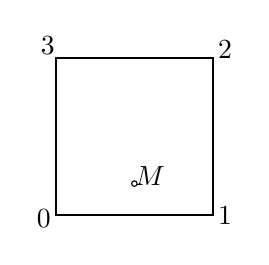
\begin{tikzpicture}
%\draw[step=0.5cm,gray,very thin] (0,0) grid (4,4); %background grid
\draw[thick] (1,1) -- (3,1) -- (3,3) -- (1,3) -- cycle;  
\node[] at (0.85,0.95) {0};
\node[] at (3.15,1) {1};
\node[] at (3.15,3.1) {2};
\node[] at (0.9,3.15) {3};
\node[] at (2.2,1.5) {$M$};
\draw (2.,1.4) circle (1pt);
\end{tikzpicture}\\
\end{center}


%..................................................
\paragraph{An intermediate case} We make the following assumption that the lateral sides of the  
element are vertical while the bottom and top are not necessarily horizontal:

\begin{center}
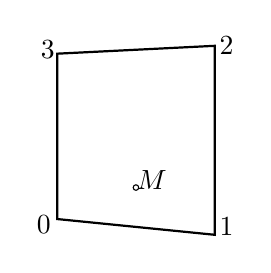
\begin{tikzpicture}
%\draw[step=0.5cm,gray,very thin] (0,0) grid (4,4); %background grid
\draw[thick] (1,1) -- (3,0.8) -- (3,3.2) -- (1,3.1) -- cycle;  
\node[] at (0.83,0.93) {0};
\node[] at (3.15,0.9) {1};
\node[] at (3.15,3.2) {2};
\node[] at (0.88,3.15) {3};
\node[] at (2.2,1.5) {$M$};
\draw (2.,1.4) circle (1pt);
\end{tikzpicture}\\
\end{center}

\noindent Because the sides are verical then if $x_0 \leq x_M \leq x_2$ then 
\[
r_M = \frac{2}{x_2-x_0}(x_M-x_0) -1 
\]
Then, if $M$ is inside the element then its $y$ coordinate is given by
\[
y_M = \sum_i \bN_i(r_M,s_M) y_i
\]
where $\bN_i$ are the four $Q_1$ basis functions associated to the vertices.
Assuming we know $r_M$ then we can solve for $s_M$:
\begin{eqnarray}
y_M &=&  
\frac{1}{4}(1-r_M)(1-s_M) y_0+
\frac{1}{4}(1+r_M)(1-s_M) y_1+
\frac{1}{4}(1+r_M)(1+s_M) y_2+
\frac{1}{4}(1-r_M)(1+s_M) y_3 \nn\\
&=& 
\frac{1}{4} \left[
(1-r)y_0+(1+r)y_1+(1+r)y_2+(1-r)y_3 +s_M [ -(1-r)y_0 - (1+r)y_1+(1+r)y_2+(1-r)y_3  ] 
\right] \nn 
\end{eqnarray}
or, 
\[
s_M = \frac{ 4y_M - [(1-r_M)y_0+(1+r_M)y_1+(1+r_M)y_2+(1-r_M)y_3]  }{ -(1-r_M)y_0 -(1+r_M)y_1+(1+r_M)y_2+(1-r_M)y_3 } 
\]
If the obtained value is in $[-1,1]$ then the point $M$ is in the element.
Verification: when $y_1=y_0$ and $y_2=y_3$ then 
\begin{eqnarray}
s_M 
&=& \frac{4 y_M - [(1-r_M)y_0+(1+r_M)y_0+(1+r_M)y_3+(1-r_M)y_3]  }{ -(1-r_M)y_0 - (1+r_M)y_0+(1+r_M)y_3+(1-r_M)y_3 } \nn\\
&=& \frac{4 y_M - [ 2 y_0 + 2 y_3]  }{ -2 y_0 + 2 y_3    }  \nn\\
&=& \frac{1}{y_3-y_0} [2 y_M - (  y_0 +  y_3) ] \nn\\ 
&=& \frac{1}{y_3-y_0} [2 y_M -  2 y_0 +y_0 -  y_3)  ] \nn\\ 
&=& \frac{2}{y_3-y_0} (y_M - y_0) - 1 
\end{eqnarray}
which is the expression that corresponds to a rectangular element as seen previously.

%..................................................
\paragraph{A generic quadrilateral}

We wish to arrive at a single algorithm which is applicable to all quadrilaterals and we now focus  
on an irregular quadrilateral (no face is parallel to the axis of the coordinate system). 

\begin{center}
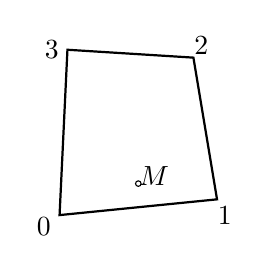
\begin{tikzpicture}
%\draw[step=0.5cm,gray,very thin] (0,0) grid (4,4); %background grid
\draw[thick] (1,1) -- (3,1.2) -- (2.7,3) -- (1.1,3.1) -- cycle;  
\node[] at (0.8,0.85) {0};
\node[] at (3.1,1) {1};
\node[] at (2.8,3.15) {2};
\node[] at (0.9,3.1) {3};
\node[] at (2.2,1.5) {$M$};
\draw (2.,1.4) circle (1pt);
\end{tikzpicture}\\
\end{center}

\noindent Several rather simple options exist:
\begin{itemize}
\item we could subdivide the quadrilateral into two triangles and check whether point $M$ is inside any of them (as it turns out, this problem is rather straightforward for triangles. Simply google it.)
\item We could check that point $M$ is always on the left side of segments $0\rightarrow 1$, $1\rightarrow 2$, $2\rightarrow 3$, $3\rightarrow 0$.
\item ...  
\end{itemize}

Any of these approaches will work although some might be faster than others. 
In three-dimensions all will however become 
cumbersome to implement and might not even work at all. 
Fortunately, there is an elegant way to answer the question, as 
detailed in the following subsection, which works both in 2D and 3D.

%-------------------------------------------
\subsubsection{Three-dimensional space}

If point $M$ is inside the quadrilateral, there exist a set of reduced 
coordinates $r,s,t\in[-1:1]^3$ such that 

\[
\sum_{i=1}^4 \bN_i(r_M,s_M,t_M) x_i = x_M
\quad\quad\quad
\sum_{i=1}^4 \bN_i(r_M,s_M,t_M) y_i = y_M
\quad\quad\quad
\sum_{i=1}^4 \bN_i(r_M,s_M,t_M) z_i = z_M
\]
This can be cast as a system of three equations and three unknowns. 
Unfortunately, each basis function $\bN_i$ 
contains a term $rst$ (as well as $rs$, $rt$, and $st$) 
so that it is not a linear system.
We must then use an iterative technique: the algorithm starts with 
a guess for values $r_M,s_M,t_M$ and 
improves on their value iteration after iteration. 
In what follows the subscript $M$ is dropped from $r,s,t$.

The classical way of solving nonlinear systems of equations is Newton's method. 
\index{general}{Newton's method}
We can rewrite the equations above as ${\bm F}(r,s,t)=0$:
\begin{eqnarray}
\sum_{i=1}^8 \bN_i(r,s,t) x_i - x_M&=&0 \nonumber\\
\sum_{i=1}^8 \bN_i(r,s,t) y_i - y_M&=&0 \nonumber\\
\sum_{i=1}^8 \bN_i(r,s,t) z_i - z_M&=&0
\end{eqnarray}
or,
\begin{eqnarray}
F_r(r,s,t)&=&0 \nonumber\\
F_s(r,s,t)&=&0 \nonumber\\
F_t(r,s,t)&=&0 \nonumber
\end{eqnarray}
so that we now have to find the zeroes of continuously differentiable 
functions ${\bm F}:\mathbb{R} \rightarrow \mathbb{R}$.
The recursion is simply:
\[
\left(
\begin{array}{c}
r_{k+1} \\s_{k+1} \\ t_{k+1}
\end{array}
\right)
=
\left(
\begin{array}{c}
r_{k} \\s_{k} \\ t_{k}
\end{array}
\right)
- J_F(r_k,s_k,t_k) ^{-1} 
\left(
\begin{array}{c}
F_r(r_k,s_k,t_k) \\
F_s(r_k,s_k,t_k)\\
F_t(r_k,s_k,t_k)
\end{array}
\right)
\]
where $J$ the Jacobian matrix:
\begin{eqnarray}
J_F(r_k,s_k,t_k)
&=&
\left(
\begin{array}{ccc}
\frac{\partial F_r}{\partial r}(r_k,s_k,t_k) & \frac{\partial F_r}{\partial s}(r_k,s_k,t_k) & \frac{\partial F_r}{\partial t}(r_k,s_k,t_k) \\\\
\frac{\partial F_s}{\partial r}(r_k,s_k,t_k) & \frac{\partial F_s}{\partial s}(r_k,s_k,t_k) & \frac{\partial F_s}{\partial t}(r_k,s_k,t_k) \\\\
\frac{\partial F_t}{\partial r}(r_k,s_k,t_k) & \frac{\partial F_t}{\partial s}(r_k,s_k,t_k) & \frac{\partial F_t}{\partial t}(r_k,s_k,t_k) 
\end{array}
\right) \nonumber\\
&=&
\left(
\begin{array}{ccc}
\sum\limits_{i=1}^8 \frac{\partial \bN_i}{\partial r}(r_k,s_k,t_k) x_i &
\sum\limits_{i=1}^8 \frac{\partial \bN_i}{\partial s}(r_k,s_k,t_k) x_i &
\sum\limits_{i=1}^8 \frac{\partial \bN_i}{\partial t}(r_k,s_k,t_k) x_i \\
\sum\limits_{i=1}^8 \frac{\partial \bN_i}{\partial r}(r_k,s_k,t_k) y_i &
\sum\limits_{i=1}^8 \frac{\partial \bN_i}{\partial s}(r_k,s_k,t_k) y_i &
\sum\limits_{i=1}^8 \frac{\partial \bN_i}{\partial t}(r_k,s_k,t_k) y_i \\
\sum\limits_{i=1}^8 \frac{\partial \bN_i}{\partial r}(r_k,s_k,t_k) z_i &
\sum\limits_{i=1}^8 \frac{\partial \bN_i}{\partial s}(r_k,s_k,t_k) z_i &
\sum\limits_{i=1}^8 \frac{\partial \bN_i}{\partial t}(r_k,s_k,t_k) z_i 
\end{array}
\right) \nonumber 
\end{eqnarray}
In practice, we solve the following system:
\[
J_F(r_k,s_k,t_k) 
\left[  
\left(
\begin{array}{c}
r_{k+1} \\s_{k+1} \\ t_{k+1}
\end{array}
\right)
-
\left(
\begin{array}{c}
r_{k} \\s_{k} \\ t_{k}
\end{array}
\right)
\right]=-
\left(
\begin{array}{c}
F_r(r_k,s_k,t_k) \\
F_s(r_k,s_k,t_k)\\
F_t(r_k,s_k,t_k)
\end{array}
\right)
\]
Finally, the algorithm goes as follows:
\begin{itemize}
\item set guess values for $r,s,t$ (typically 0)
\item loop over k=0,...
\item Compute rhs= $-{\bm F}(r_k,s_k,t_k)$ 
\item Compute matrix $J_F(r_k,s_k,t_k)$
\item solve system for $(dr_k,ds_k,dt_k)$
\item update $r_{k+1}=r_k+dr_k$, $s_{k+1}=s_k+ds_k$, $t_{k+1}=t_k+dt_k$ 
\item stop iterations when $(dr_k,ds_k,dt_k)$ is small
\item if $r_k,s_k,t_k\in[-1,1]^3$ then $M$ is inside.
\end{itemize}
This method converges quickly but involves iterations, and multiple 
solves of $3\times 3$ systems which, when carried out for each marker 
and at each time step can prove to be expensive. 
A simple modification can be added to the above algorithm: 
iterations should be carried out {\it only}
when the point $M$ is inside of a cuboid of 
size $[\min\limits_i{x_i}:\max\limits_i{x_i}]\times[\min\limits_i{y_i}:\max\limits_i{y_i} ]
\times[\min\limits_i{z_i}:\max\limits_i{z_i}]$ where the sums run over the vertices of the element. 
In 2D this translates as follows: only carry out Newton iterations when $M$ is inside the red rectangle!
\begin{center}
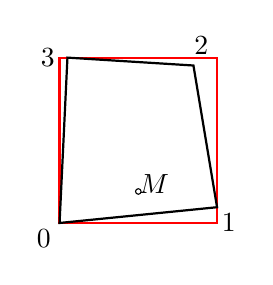
\begin{tikzpicture}
%\draw[step=0.5cm,gray,very thin] (0,0) grid (4,4); %background grid
\draw[thick,red] (1,1) -- (3,1) -- (3,3.1) -- (1,3.1) -- cycle;  
\draw[thick] (1,1) -- (3,1.2) -- (2.7,3) -- (1.1,3.1) -- cycle;  
\node[] at (0.8,0.8) {0};
\node[] at (3.15,1) {1};
\node[] at (2.8,3.25) {2};
\node[] at (0.85,3.1) {3};
\node[] at (2.2,1.5) {$M$};
\draw (2.,1.4) circle (1pt);
\end{tikzpicture}\\
\end{center}

Note that the algorithm above extends to high degree elements 
such as $Q_2$ and higher, even with curved sides.
As shown in the 2D case if the element is a cuboid or 
if all its lateral faces are vertical then one can 
compute the reduced coordinates without using an iterative method.


%-----------------------------------------------------
\subsubsection{Three-dimensional space - special case}

We assume that the mesh is such that the cross section of all $Q_1$ elements 
is a rectangle in the $xy$-plane. 

Let $(x,y,z)$ be a point inside the element. 
The global coordinates $x,y,z$ are obtained from the 
reduced coordinates $r,s,t$ via the basis the basis functions:
\begin{eqnarray}
x=\sum_{i=1}^8 \bN_i (r,s,t) x_i \qquad 
y=\sum_{i=1}^8 \bN_i (r,s,t) y_i  \qquad 
z=\sum_{i=1}^8 \bN_i (r,s,t) z_i \label{xyz}
\end{eqnarray}
Let 
\begin{eqnarray}
{\vec v}_1 &=& (+1,+1,+1,+1,+1,+1,+1,+1) \nn\\
{\vec v}_2 &=& (-1,+1,+1,-1,-1,+1,+1,-1) \nn\\
{\vec v}_3 &=& (-1,-1,+1,+1,-1,-1,+1,+1) \nn\\
{\vec v}_4 &=& (-1,-1,-1,-1,+1,+1,+1,+1) \nn\\
{\vec v}_5 &=& (+1,-1,+1,-1,+1,-1,+1,-1) \nn\\
{\vec v}_6 &=& (+1,-1,-1,+1,-1,+1,+1,-1) \nn\\
{\vec v}_7 &=& (+1,+1,-1,-1,-1,-1,+1,+1) \nn
\end{eqnarray}
and 
\begin{eqnarray}
{\vec x} &=& (x_1,x_2,x_3,x_4,x_5,x_6,x_7,x_8) \nn\\
{\vec y} &=& (y_1,y_2,y_3,y_4,y_5,y_6,y_7,y_8) \nn\\
{\vec z} &=& (z_1,z_2,z_3,z_4,z_5,z_6,z_7,z_8) \nn
\end{eqnarray}
then Eqs.~\eqref{xyz} can also be written
\begin{eqnarray}
x&=&\frac{1}{8} \left( {\vec v}_1 + r  {\vec v}_2 + s  {\vec v}_3 + t  {\vec v}_4 
                 + rs  {\vec v}_5 + rt {\vec v}_6 + st {\vec v}_7 \right) \cdot {\vec x} \nn\\ 
y&=&\frac{1}{8} \left( {\vec v}_1 + r  {\vec v}_2 + s  {\vec v}_3 + t  {\vec v}_4 
                 + rs  {\vec v}_5 + rt {\vec v}_6 + st {\vec v}_7 \right) \cdot {\vec y} \nn\\
z&=&\frac{1}{8} \left( {\vec v}_1 + r  {\vec v}_2 + s  {\vec v}_3 + t  {\vec v}_4 
                 + rs  {\vec v}_5 + rt {\vec v}_6 + st {\vec v}_7 \right) \cdot {\vec z} \label{zzz}
\end{eqnarray}
If the element has a rectangular cross-section $s_x \times s_y$ then 
\begin{eqnarray}
{\vec x} &=& (x_0,x_0+s_x,x_0+s_x,x_0,x_0,x_0+s_x,x_0+s_x,x_0) \nn\\
{\vec y} &=& (y_0,y_0,y_0+s_y,y_0+s_y,y_0,y_0,y_0+s_y,y_0+s_y) \nn
\end{eqnarray}
which yields
\begin{eqnarray}
r&=& 2\frac{x-x_0}{s_x}-1  \nn\\
s&=& 2\frac{y-y_0}{s_y}-1  \nn
\end{eqnarray}
Since the local coordinates $r$ and $s$ can be easily computed, one can use Eq.~\eqref{zzz} to obtain $t$:
\[
t=\frac{8z - ({\vec v}_1 + r {\vec v}_2 + s {\vec v}_3 + rs  {\vec v}_5 ) \cdot {\vec z}} 
{ ({\vec v}_4  + r  {\vec v}_6 + s  {\vec v}_7)  \cdot {\vec z} }
\]







 %---------
\newpage %-----------------------------------------------------------------------------------------
\section{Error measurements and convergence rates} \index{general}{$L_1$ norm}
\index{general}{$L_2$ norm}
\index{general}{$H^1$ norm}
\begin{flushright} {\tiny {\color{gray} errors.tex}} \end{flushright}

What follows is written in the case of a two-dimensional model. Generalisation to
3D is trivial. What follows is mostly borrowed from \cite{thmk14}.

When measuring the order of accuracy of the primitive variables $\vec{v}$ and $p$,
it is standard to report errors in both the $L_1$ and the $L_2$ norm.
For a scalar quantity $\Psi$, the $L_1$ and $L_2$ norms are computed as
\begin{equation}
\norm{\Psi}_1 = \int_V |\Psi| dV
\quad\quad
\quad\quad
\norm{\Psi}_2 = \sqrt{ \int_V \Psi^2 dV }
\end{equation}
For a vector quantity $\vec{k}=(k_x,k_y)$ in a two-dimensional space,
the $L_1$ and $L_2$ norms are defined as:
\begin{equation}
\norm{\vec{k}}_1 = \int_V (|k_x|+|k_y|) dV
\quad\quad
\quad\quad
\norm{\vec{k}}_2 = \sqrt{ \int_V (k_x^2+k_y^2) dV }
\end{equation}
To compute the respective norms
the integrals in the above norms can be approximated by splitting them
into their element-wise contributions. The element volume integral can then
be easily computed by numerical integration using Gauss-Legendre quadrature.

The respective $L_1$ and $L_2$ norms for the pressure error can be evaluated via
\begin{equation}
e_p^h|_1 = \sum_{i=1}^{n_e} \sum_{q=1}^{n_q} |e_p^h(\vec{r}_q)| w_q |J_q|
\quad\quad
\quad\quad
e_p^h|_2=\sqrt{ \sum_{i=1}^{n_e} \sum_{q=1}^{n_q} |e_p^h(\vec{r}_q)|^2 w_q |J_q| }
\end{equation}
where $e_p^h(\vec{r}_q)=p^h(\vec{r}_q) - p(\vec{r}_q)$ 
is the pressure error evaluated at the $q$-th quadrature associated with
the $i$th element. $n_e$ and $n_q$ refer to the number of elements and
the number of quadrature points per element.
$w_q$ and $J_q$ are the quadrature weight and the Jacobian associated with
point $q$.

The velocity error $e_{\vec v}^h$ is evaluated using the following two norms
\begin{equation}
e_{\vec{v}}^h|_1 = \sum_{i=1}^{n_e} \sum_{q=1}^{n_q} [ |e_u^h(\vec{r}_q)| + |e_v^h(\vec{r}_q)| ]    w_q |J_q|
\quad\quad
\quad\quad
e_{\vec v}^h|_2=\sqrt{ \sum_{i=1}^{n_e} \sum_{q=1}^{n_q} \left[ |e_u^h({\bm r}_q)|^2 +  e_v^h({\bm r}_q)|^2 \right] w_q |J_q| }
\end{equation}
where $e_u^h(\vec{r}_q)=u^h(\vec{r}_q) - u(\vec{r}_q)$ and $e_v^h(\vec{r}_q)=v^h(\vec{r}_q)-v(\vec{r}_q)$.


\index{general}{$H^1(\Omega)$ space} 
\index{general}{$H^1$ norm} 
\index{general}{$H^1$ semi-norm}
Another norm is very rarely used in the geodynamics literature but is preferred in the 
Finite Element literature: the $H^1$ norm. The mathematical basis for this
norm and the nature of the $H^1(\Omega)$ Hilbert space is to be found in many FE books \cite{dohu03,john16,hugh}.
This norm is expressed as follows for a function $f$ such that $f,|\nabla f|\in L^2(\Omega)$
\footnote{\url{https://en.wikipedia.org/wiki/Sobolev_space}}
\begin{equation}
\norm{f}_{H^1} = \left( \int_\Omega ( |f|^2 + |\nabla f|^2  ) d\Omega   \right)^{1/2}
\end{equation}
We then have 
\begin{equation}
e_{\vec v}^h|_{H^1} = \norm{\vec{v}^h-\vec{v}}_{H^1} = \sqrt{
\sum\limits_{i=1}^d 
\int_\Omega  
\left[
({v}_i^h-{v}_i)^2
+
\vec\nabla(v_i^h-v_i)\cdot\vec\nabla(v_i^h-v_i) 
\right] d\Omega   
}
\end{equation}
where $d$ is the number of dimensions.
Note that sometimes the following semi-norm is used \cite{dobo04,bodg06}:
\begin{equation}
e_{\vec v}^h|_{H^1} = \norm{\vec{v}^h-\vec{v}}_{H^1} = \sqrt{
\sum\limits_{i=1}^d 
\int_\Omega  
\left[
\vec\nabla(v_i^h-v_i)\cdot\vec\nabla(v_i^h-v_i) 
\right] d\Omega   
}
\end{equation}

When computing the different error norms for $e_p$ and $e_{\vec v}$ for a set of numerical experiments with
varying resolution $h$ we expect the error norms to follow the following relationships:
\begin{equation}
e_{\vec v}^h|_1 = C h^{rvL_1} 
\quad\quad\quad\quad
e_{\vec v}^h|_2 = C h^{rvL_2} 
\quad\quad\quad\quad 
e_{\vec v}^h|_{H^1} = C h^{rvH^1}
\end{equation}
\begin{equation}
e_p^h|_1 = C h^{rpL_1} 
\quad\quad\quad 
e_p^h|_2 = C h^{rpL_2}
\end{equation}
where $C$ is a resolution-independent constant
and $rpXX$ and $rvXX$ are the convergence rates for
pressure and velocity in various norms, respectively. 
Using linear regression on the logarithm of the respective error norm and the resolution $h$,
one can compute the convergence rates of the numerical solutions.

As mentioned in \cite{dobo04}, when finite element solutions converge at
the same rates as the interpolants we say that the method is optimal, i.e.:
\index{general}{optimal rate}

\begin{equation}
e_{\vec v}^h|_{L_2} = {\cal O}(h^3)
\quad\quad\quad\quad
e_{\vec v}^h|_{H^1} = {\cal O}(h^2)
\quad\quad\quad\quad
e_{p}^h|_{L_2} = {\cal O}(h^2)
\end{equation}

%\begin{itemize}
%\item For $Q_1P_0$, the theoretical lower bound for $r_v'$ is 2 and for $r_p'$ it is 1
%\item For $Q_2P_{-1}$, the theoretical lower bound for $r_v'$ is 3 and for $r_p'$ it is 2
%\end{itemize}
We note that when using discontinuous pressure space
(e.g., $P_0$, $P_{-1}$), these bounds remain valid even
when the viscosity is discontinuous provided that the element boundaries conform to the discontinuity.

%------------------------------------------------------------------------------ 
\subsubsection{About extrapolation}\label{ss:extrapolation}
\index{general}{Extrapolation}

Section contributed by W. Bangerth and part of \textcite{thba22} (2022) 
but it was ultimately not used. 

In a number of numerical benchmarks we
want to estimate the error $X_h-X^\ast$ between a quantity $X_h$ computed
from the numerical solution $\vec{\upnu}_h,p_h$ and the corresponding value
$X$ computed from the exact solution $\vec{\upnu},p$. Examples of such quantities
$X$ are the root mean square velocity $\upnu_{rms}$, but it could also be a mass flux
across a boundary, an average horizontal velocity at the top boundary, or
any other scalar quantity.

If the exact solution is known, then one can of course compute $X$ from it.
On the other hand, we would of course like to assess convergence also in
cases where the exact solution is not known. In that case, one can compute
an \textit{estimate} $X^\ast$ for $X$ by way of \textit{extrapolation}.
To this end, we make the assumption that asymptotically, $X_h$ converges to
$X$ at a fixed (but unknown) rate $r$, so that
\begin{equation}
  \label{eq:extrapolation-1}
  e_h=|X_h-X| \approx C h^r.
\end{equation}
Here, $X$, $C$ and $r$ are all unknown constants to be determined, although
we are not really interested in $C$.
We can evaluate $X_h$ from the numerical solution
on successively refined meshes with mesh sizes $h$, $h/2$, and $h/4$. Then,
in addition to \eqref{eq:extrapolation-1} we also have
\begin{eqnarray}
  \label{eq:extrapolation-2}
  e_{h/2}=|X_{h/2}-X| \approx C \left(\frac h2\right)^r,
  \\
  \label{eq:extrapolation-3}
  e_{h/4} =|X_{h/4}-X| \approx C \left(\frac h4\right)^r.
\end{eqnarray}
Taking ratios of equations \eqref{eq:extrapolation-1}--\eqref{eq:extrapolation-3},
and replacing the unknown $X$ by an \textit{estimate} $X^\ast$, we then
arrive at the following equation:
\begin{equation*}
\frac{|X_h-X^\star|}{|X_{h/2}-X^\star|}
=
\frac{|X_{h/2}-X^\star|}{|X_{h/4}-X^\star|}=2^r.
\end{equation*}
If one assumes that $X_h$ converges to $X$ uniformly either from above or
below (rather than oscillate around $X$), then this equation allows us
to solve for $X^\ast$ and $r$:

\[
(X_h-X^\star)(X_{h/4}-X^\star)=(X_{h/2}-X^\star)(X_{h/2}-X^\star)
\]

\[
X_h X_{h/4} -X^\star  X_{h/4} - X_h X^\star  + (X^\star)^2
=X_{h/2}^2 -2 X^\star X_{h/2} + (X^\star)^2 
\]

\[
X_h X_{h/4} -X^\star  X_{h/4} - X_h X^\star 
=X_{h/2}^2 -2 X^\star X_{h/2} 
\]

\[
X_h X_{h/4} -X_{h/2}^2 =-2 X^\star X_{h/2} +X^\star  X_{h/4} + X_h X^\star 
\]

\[
X_h X_{h/4} -X_{h/2}^2  = X^\star ( -2  X_{h/2}  +   X_{h/4} + X_h )
\]

and finally:
\begin{equation*}
X^\star = \frac{X_h X_{h/4}-X_{h/2}^2}{X_h - 2 X_{h/2} + X_{h/4}}, \qquad\qquad
r = \log_2 \frac{X_{h/2}-X^\star}{X_{h/4}-X^\star}.
\end{equation*}
In the determination of $r$, we could also have used $X_h$ and $X_{h/2}$,
but using $X_{h/2}$ and $X_{h/4}$ is generally more reliable because
the higher order terms we have omitted in \eqref{eq:extrapolation-1} are less
visible on finer meshes.

In some cases, however, halving the mesh size multiple times 
is not really tractable (memory problem, or cpu time).
Let us now start again from 
\begin{equation}
  e_h=|X_h-X| \approx C h^r.
\end{equation}
and assume that we run two other models at a resolution $\alpha h$
and $\beta h$, such that $1>\alpha>\beta>0$. 
In the example above we of course had $\alpha=1/2$ and $\beta=1/4$.
Then we have 
\begin{eqnarray}
e_{\alpha h}=|X_{\alpha h}-X| \approx C \left(\alpha h\right)^r,  \\
e_{\beta  h}=|X_{\beta h} -X| \approx C \left(\beta  h\right)^r.
\end{eqnarray}
which leads to 
\begin{equation*}
\frac{|X_h-X^\star|}{|X_{\alpha h}-X^\star|}
= \frac{C h^r}{C (\alpha h)^r} = (1/\alpha)^{r}
\qquad
\text{and}
\qquad
\frac{|X_{\alpha h}-X^\star|}{|X_{\beta h}-X^\star|}
= \frac{C (\alpha h)^r}{C(\beta h)^r} = (\alpha/\beta)^r
\end{equation*}
In order for both to be equal we must have
\[
(1/\alpha)^{r} = (\alpha/\beta)^r
\qquad
\Rightarrow
\qquad
1/\alpha = \alpha/\beta
\qquad
\Rightarrow
\qquad
\beta=\alpha^2
\]
So of course if $\alpha=1/2$ then $\beta=1/4$, but now we can also take 
$\alpha=3/4$ and then $\beta=9/16$. Etc ...

In the end, this approach might not be that useful since the mesh sizes would
then be $h,3h/4,9h/16,27h/64,...$ which may be hard to achieve in practice.

 %-----------------------------
\newpage %-----------------------------------------------------------------------------------------
\section{The initial temperature field} 
\Literature: 
\begin{itemize}
\item
Thermal gradients in the continental crust \cite{chap86}
\item
Simple analytical approximation to the temperature structure in
subduction zones \cite{enwi04}
\item 
Thermal structure of subduction zone back arcs \cite{cuhy06}
\item 
Thermal Structure of Oceanic Lithosphere \cite{rihc18}
\item thermal structure of a subducting plate with finite length \cite{hstt90}
\end{itemize}


%.............................................................
\subsubsection{Single layer with imposed temperature b.c.}

Let us take a single layer of material characterised by
a heat capacity $C_p$, a heat conductivity $k$
and a heat production term $H$.

\begin{center}
\includegraphics[width=5cm]{images/initial_temperature/tempcond.png}
\end{center}

The Heat transport equation writes
\begin{equation}
\rho C_p \left( \frac{\partial T}{\partial t} + {\vec v} \cdot {\vec \nabla} { T} \right) = 
{\vec \nabla} \cdot (k {\vec \nabla} T) + \rho H
\end{equation}
At steady state and in the absence of a velocity field, assuming
that the material properties to be independent of time and space, and 
assuming that
there is no heat production ($H=0$), this equation
simplifies to
\begin{equation}
\Delta T =0 
\end{equation}
Assuming the layer to be parallel to the $x$-axis, the temperature is
$T(x,y)=T(y)=\alpha T+ \beta$. 
In order to specify the constants $\alpha$ and $\beta$, we need two constraints.

At the bottom of the layer $y=y_b$ a temperature $T_b$ is prescribed while a temperature
$T_t$ is prescribed at the top with $y=y_t$. This ultimately yields a temperature field in
the layer given by
\begin{mdframed}[backgroundcolor=blue!5]
\[
T(y) = \frac{T_t-T_b}{y_t-y_b}(y-y_b) + T_b
\]
\end{mdframed}

If now the heat production coefficient is not zero, the differential equation
reads
\begin{equation}
 k \Delta T + H = 0 
\end{equation}
The temperature field is then expected to be of the form
\begin{equation}
T(y)= - \frac{H}{2k} y^2 + \alpha y + \beta 
\end{equation}
Supplied again with the same boundary conditions, this leads to
\[
\beta=T_b + \frac{H}{2k} y_b^2 - \alpha y_b
\]
ie,
\[
T(y) = -\frac{H}{2k} (y^2-y_b^2) + \alpha (y-y_b) + T_b
\]
and finally
\[
\alpha =  \frac{T_t-T_b}{y_t-y_b}  + \frac{H}{2k}(y_b+y_t)
\]
or,
\[
T(y) = -\frac{H}{2k} (y^2-y_b^2) + \left( \frac{T_t-T_b}{y_t-y_b}  + \frac{H}{2k}(y_b+y_t)   \right) (y-y_b) + T_b
\]

Taking $H=0$ in this equation obviously yields the temperature field obtained previously.
Taking $k=2.25$, $T_t=0C$, $T_b=550C$, $y_t=660km$, $y_b=630km$ yields the following
temperature profiles and heat fluxes when the heat production $H$ varies:
\begin{center}
\includegraphics[width=5cm]{images/initial_temperature/temperature1.pdf}
\includegraphics[width=5cm]{images/initial_temperature/heatflux1.pdf}
\end{center}
Looking at the values at the top, which are somewhat estimated to be
about $55-65mW/m^2$ \cite[table 8.6]{jama}, one sees that value $H=0.8e-6$ yields a very acceptable
heat flux.
Looking at the bottom, the heat flux is then about $0.03W/m^2$
which is somewhat problematic since the heat flux at the Moho
is reported to be somewhere between 10 and 20 $mW/m^2$ in \cite[table 7.1]{jama}.


%-----------------------------------------------------
\subsubsection{Single layer with imposed heat flux b.c.}

Let us now assume that heat fluxes are imposed at the top and bottom of the layer:
\begin{center} 
\includegraphics[width=5cm]{images/initial_temperature/tempcond2.png}
\end{center}

We start again from the ODE
\[
k \Delta T + H = 0 
\]
but only integrate it once:
\[
k \frac{dT}{dy}  + H y + \alpha  = 0 
\]
At the bottom $q=k(dT/dy)|_{y=y_b} = q_b$ and at the top
$q=k(dT/dy)|_{y=y_t} = q_t$ so that 

\todo[inline]{to finish}


 
%-----------------------------------------------------
\subsubsection{Single layer with imposed heat flux and temperature b.c. }

\begin{center}
\includegraphics[width=5cm]{images/initial_temperature/tempcond3.png}
\end{center}

\todo[inline]{to finish}


%---------------------------------------------------------------
\subsubsection{Half cooling space}

TODO. 

\Literature \cite{fagm12} 

%---------------------------------------------------------------
\subsubsection{Plate model}

\cite{mcke67}

%.................................
\subsubsection{McKenzie slab}

When doing thermo-mechanical modelling, the initial temperature
field in the domain is of prime importance. This is 
especially true for the temperature in the slab for subduction 
modelling as its rheological behaviour is strongly temperature-dependent. 
One could easily design a simple geometrical initial field but it is 
unlikely to be close to the field of a slowly subducting slab at an angle 
in a hot mantle. 

McKenzie \cite{mcke69} derived such approximate initial field from the 
steady-state energy equation in two dimensions:
\begin{equation}
\rho C_p \vec v \cdot \vec\nabla T = k \vec\nabla^2 T
\end{equation}
We denote by $T_l$ the temperature at the base of the lithosphere
and $l$ its thickness (i.e. the thickness of the slab).

Assuming $\vec v=(v_x,0)$ yields
\[
\rho C_p v_x \frac{\partial T}{\partial x} = k \frac{\partial^2 T}{\partial x^2}
\]
and substitution of $T'=T/T_l$, $x'=x/l$ and $z'=z/l\in[0,1]$ in this equation leads to
\[
\rho C_p v_x \frac{T_l}{l}\frac{\partial T'}{\partial x'} = k \frac{T_l}{l^2}
\left( \frac{\partial^2 T'}{\partial x'^2}
+ \frac{\partial^2 T'}{\partial z'^2} \right)
\]
or 
\[
\frac{\rho C_p v_x l }{k}\frac{\partial T'}{\partial x'} = 
\frac{\partial^2 T'}{\partial x'^2}
+ \frac{\partial^2 T'}{\partial z'^2} 
\]
and finally (see Eq. 2.3 of \cite{mcke69}): 
\[
\frac{\partial^2 T'}{\partial x'^2}
- 2 R \frac{\partial T'}{\partial x'} 
+ \frac{\partial^2 T'}{\partial z'^2} =0
\]
where $R$ is the thermal Reynolds number
\[
R=\frac{\rho C_p v_x l}{2 k}
\] 
The general solution to this PDE with $T'=1$ on the top, left and right boundary is 
\[
T'(x',z')= 1 + \sum_n C_n \exp \left[ \left( R-(R^2+n^2\pi^2)^{1/2} \right) x' \right] \sin (n \pi z')
\]
We now must make an assumption about the temperature on the left boundary ($x'=0$), 
which is the temperature of the lithosphere. 
For simplicity McKenzie assumes that $T'(x'=0,z')=1-z'$ so that $C_n=2(-1)^n/n\pi$ and finally
\begin{mdframed}[backgroundcolor=blue!5]
\begin{equation}
T'(x',z')= 1 + 2\sum_n \frac{(-1)^n}{n \pi} \exp \left[ \left( R-(R^2+n^2\pi^2)^{1/2} \right) x' \right] \sin (n \pi z')
\end{equation}
\end{mdframed}

Let us build a simple temperature model for a $250\text{km}\times 50\text{km}$ slab, 
with $\rho=3000$, $C_p=1250$, $k=3$. The python code is available in {\tt images/mckenzie/mckenzie1.py}.

\begin{center}
\includegraphics[width=0.32\textwidth]{images/mckenzie/temperature_vel0p5.pdf}
\includegraphics[width=0.32\textwidth]{images/mckenzie/temperature_vel1.pdf}
\includegraphics[width=0.32\textwidth]{images/mckenzie/temperature_vel2.pdf}\\
{\captionfont Left to right: Dimensionless temperature $T'$ in a $250\text{km}\times 50\text{km}$ slab 
for $v_x={0.5,1,2}\text{cm/year}$}
\end{center}

We logically recover the fact that the slower the slab penetrates the mantle the more 
temperature diffusion dominates over temperature advection. For $v=0.5\text{cm/year}$ we see that 
that the slab assumes a constant temperature $T'=1$ at all depthes $0\leq z' \leq 1$ for 
$x'\geq 125\text{km}$. 

Note that this field is a steady-state field, valid for a constant density, heat conductivity and 
heat capacity, zero heat production, that it implies that the velocity is constant and that the 
lithosphere temperature is linear. 

One can also embed the slab in a more realistic context, a subduction zone, involving a 
subducting lithosphere, an over-riding plate and a mantle. The domain is $1000\text{km}\times 250\text{km}$.
The mantle temperature is set to $1300~\si{\celsius}$. The slab dip can be varied and so can the 
velocity. The python code is available in {\tt images/mckenzie/mckenzie2.py}.

\begin{center}
\includegraphics[width=0.32\textwidth]{images/mckenzie/temperature2_vel0p5_phi30.pdf}
\includegraphics[width=0.32\textwidth]{images/mckenzie/temperature2_vel1_phi30.pdf}
\includegraphics[width=0.32\textwidth]{images/mckenzie/temperature2_vel2_phi30.pdf}\\
{\captionfont Left to right: temperature $T$ for $v_x={0.5,1,2}\text{cm/year}$ and $\phi=30\degree$.}
\end{center}

\begin{center}
\includegraphics[width=0.32\textwidth]{images/mckenzie/temperature2_vel1_phi15.pdf}
\includegraphics[width=0.32\textwidth]{images/mckenzie/temperature2_vel1_phi30.pdf}
\includegraphics[width=0.32\textwidth]{images/mckenzie/temperature2_vel1_phi45.pdf}\\
{\captionfont Left to right: temperature $T$ for $v_x=1\text{cm/year}$ and $\phi={15,30,45}\degree$.}
\end{center}




%\newpage

%From \cite{mcke70}, Eq. 26:
%\[
%T(r_0) = \theta_1 \exp \left(  \frac{\alpha g}{C_p} (r_1-r_0) \right)
%\]
%where $\theta_1$ is the potential temperature of any piece of the mantle 
%at the earth's surface.
%If $x$ is measured from a depth equal to the thickness of the lithosphere down the
%dip of the slab and $z$ is measured along the normal to the slab from its lower 
%surface, then the dimensionless potential temperature in the slab is 
%\begin{eqnarray}
%\theta'(x',z')
%&=& 1+2\frac{\theta_1-273}{\theta_1} \sum_{n=1}^\infty \frac{(-1)^n}{n \pi}
%\exp \left[ \left( R-(R^2+n^2\pi^2)^{1/2} \right) x' \right] \sin n\pi z' \\
%&=& \frac{1}{\theta_1} \left\{ \theta_1+ 2 (\theta_1-273) \sum_{n=1}^\infty \frac{(-1)^n}{n \pi}
%\exp \left[ \left( R-(R^2+n^2\pi^2)^{1/2} \right) x' \right] \sin n\pi z' \right\}
%\end{eqnarray}
%where $\theta' = \theta/\theta_1$, $x'=x/l$, $z'=z/l$ and 
%with $l$ the thickness of the slab and $v$ its velocity measured down its dip.
%We denote by $\phi$ the dip of the slab so that the depth below the surface $r_1-r_0$ is given by
%$l (x' \sin \phi-z' \cos\phi)$ so that 
%\[
%T(r_0) = \theta_1 \exp \left(  \frac{\alpha g}{C_p} l (x' \sin \phi-z' \cos\phi) \right)
%\]
%The dimensionless scale height $h'$ is defined by $h'=C_p/\alpha g l$ so that
%\[
%T(r_0) = \theta_1 \exp \left[  (x' \sin \phi-z' \cos\phi)/h' \right]
%\]

%Finally,
%\[
%T(x',z')=\exp \left[  (x' \sin \phi-z' \cos\phi)/h' \right] 
%\left\{ \theta_1+ 2 (\theta_1-273) \sum_{n=1}^\infty \frac{(-1)^n}{n \pi}
%\exp \left[ \left( R-(R^2+n^2\pi^2)^{1/2} \right) x' \right] \sin n\pi z' \right\}
%\]

%\todo[inline]{BSc: create mckenzie slab temperature setup}

%......................................................................
\subsubsection{Initial temperature for global mantle convection models}

This is a difficult topic, and Gottschaldt \etal \cite{gows09} list a few issues or 
facts to take into account:
\begin{itemize}
\item Frequent  impacts  may  have  determined  the  heat structure of the outer layers (Arrhenius and Lepland 2000), leading to an early thermally stable stratification. 
\item A global magma ocean (Solomatov 2000)  or  several  large  scale  melting events  (Kleine \etal. 2004)  
are also conceivable. 
\item Fractional crystallisation and subsequent overturn has the potential to result in 
compositionally or thermally stable layering, too (Elkins-Tanton \etal 2003; Zaranek and Parmentier 2004)
\end{itemize}


 %---------------------------
\newpage %-----------------------------------------------------------------------------------------
\section{Kinematic boundary conditions}\label{kin_bc} \index{general}{Essential Boundary Conditions}
\index{general}{Natural Boundary Conditions}
\begin{flushright} {\tiny {\color{gray} kinematic\_bc.tex}} \end{flushright}


\begin{center}
\includegraphics[width=8cm]{images/boundary_conditions/bc1}
\end{center}


\begin{center}
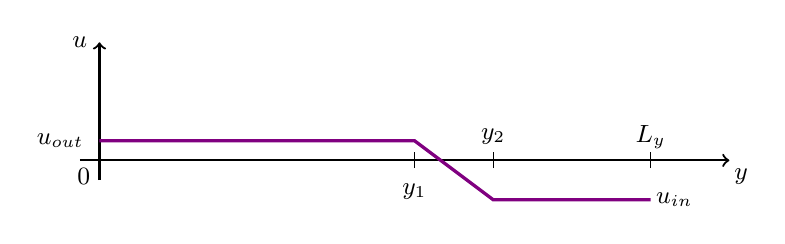
\begin{tikzpicture}
%\draw[fill=gray!23,gray!23](0,0) rectangle (10,3);
%\draw[step=0.5cm,gray,very thin] (0,0) grid (10,3); %background grid
\draw[thick,->] (0.75,1) -- (9,1)  ; 
\draw[thick,->] (1,0.75) -- (1,2.5)  ; 
\draw[-] (5,0.9) -- (5,1.1)  ; 
\draw[-] (6,0.9) -- (6,1.1)  ; 
\draw[-] (8,0.9) -- (8,1.1)  ; 
\draw[very thick, violet] (1,1.25)--(5,1.25) -- (6,0.5) -- (8,0.5) ; 
\node[] at (0.8,0.8) {\small $0$};
\node[] at (9.15,0.8) {\small $y$};
\node[] at (5,0.6) {\small $y_1$};
\node[] at (6,1.3) {\small $y_2$};
\node[] at (8,1.3) {\small $L_y$};
\node[] at (8.3,0.5) {\small $u_{in}$};
\node[] at (0.5,1.25) {\small $u_{out}$};
\node[] at (0.75,2.5) {\small $u$};
\end{tikzpicture}
\end{center}



The velocity on the side is given by
\begin{eqnarray}
u(y) &=& u_{out} \quad\quad y<y_1 \nn\\
u(y) &=& \frac{u_{in}-u_{out}}{y_2-y_1}(y-y_1) + u_{out} \quad\quad y_1<y<y_2 \nn\\
u(y) &=& u_{in} \quad\quad y>y_2 \nn
\end{eqnarray}
Note that $u_{in}$ and $u_{out}$ can be positive or negative, but 
of opposite signs.
The requirement for volume conservation is:
\[
\Phi=\int_{0}^{L_y} u(y) dy = 0
\]
Having chosen $u_{in}$ (the velocity of the plate), one can then compute $v_{out}$
as a function of $y_1$ and $y_2$.

\begin{eqnarray}
\Phi
&=&
\underbrace{\int_{0}^{y_1} u(y) dy}_{\Phi_1}  +
\underbrace{\int_{y_1}^{y_2} u(y) dy }_{\Phi_2}  +
\underbrace{\int_{y_2}^{L_y} u(y) dy }_{\Phi_3}\nn
\end{eqnarray}
with
\begin{eqnarray}
\Phi_1 &=& u_{out} y_1 \nn\\
\Phi_2 
&=& \int_{y_1}^{y_2} u(y) dy \nn\\
&=& \int_{y_1}^{y_2} \left[ \frac{u_{in}-u_{out}}{y_2-y_1}(y-y_1) + u_{out}   \right] dy \nn\\
&=& \int_{y_1}^{y_2} \frac{u_{in}-u_{out}}{y_2-y_1}(y-y_1)  dy  +   \int_{y_1}^{y_2}  u_{out} dy \nn\\
&=& \frac{u_{in}-u_{out}}{y_2-y_1} \int_{y_1}^{y_2} (y-y_1)  dy  +   (y_2-y_1) u_{out}  \nn\\
&=& \frac{u_{in}-u_{out}}{y_2-y_1} \left[ \frac12 y^2 - y_1y   \right]_{y_1}^{y_2} +   (y_2-y_1) u_{out}  \nn\\
&=& \frac{u_{in}-u_{out}}{y_2-y_1} ( \frac12 y_2^2 - y_1y_2 - \frac12y_1^2 + y_1^2 ) +   (y_2-y_1) u_{out}  \nn\\
&=& \frac{u_{in}-u_{out}}{y_2-y_1} \frac12 ( y_2^2 - 2y_1y_2 + y_1^2 ) +   (y_2-y_1) u_{out}  \nn\\
&=& \frac{u_{in}-u_{out}}{y_2-y_1} \frac12 ( y_2-y_1 )^2 +   (y_2-y_1) u_{out}  \nn\\
&=& (u_{in}-u_{out}) \frac12 ( y_2-y_1 ) +   (y_2-y_1) u_{out}  \nn\\
&=& \frac{1}{2}(u_{in}+u_{out})(y_2-y_1)  \nn\\
\Phi_3 &=& (L_y-y_2) u_{in} \nn
\end{eqnarray}
so that in the end
\begin{eqnarray}
\Phi &=& \Phi_1+\Phi_2+\Phi_3 \nn\\
&=& u_{out} [y_1 + \frac{1}{2}(y_2-y_1) ] + u_{in} [ \frac{1}{2}(y_2-y_1)  + (L_y-y_2) ] \nn\\
&=& u_{out}\frac{1}{2} (y_1 + y_2 ) + u_{in} [ L_y - \frac{1}{2}(y_1+y_2) ] \nn
\end{eqnarray}
and finally, solving for $u_{out}$
\begin{mdframed}[backgroundcolor=blue!5]
\[
u_{out} = -u_{in} \frac{ L_y - \frac{1}{2}(y_1+y_2)}{ \frac{1}{2} (y_1 + y_2 ) }
\]
\end{mdframed}


In some cases one may wish to prescribe a zero velocity 
below the 660 discontinuity (given by $y=y_1$) on the following 
figure:

\begin{center}
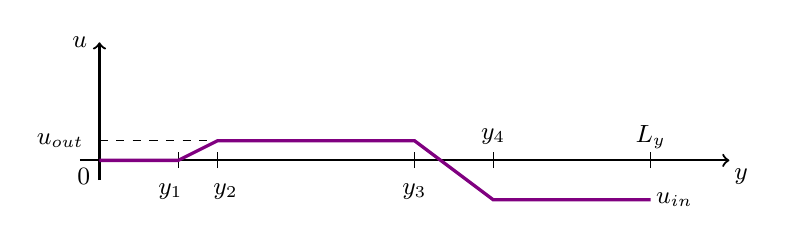
\begin{tikzpicture}
%\draw[fill=gray!23,gray!23](0,0) rectangle (10,3);
%\draw[step=0.5cm,gray,very thin] (0,0) grid (10,3); %background grid
\draw[thick,->] (0.75,1) -- (9,1)  ; 
\draw[thick,->] (1,0.75) -- (1,2.5)  ; 
\draw[-] (2,0.9) -- (2,1.1)  ; 
\draw[-] (2.5,0.9) -- (2.5,1.1)  ; 
\draw[-] (5,0.9) -- (5,1.1)  ; 
\draw[-] (6,0.9) -- (6,1.1)  ; 
\draw[-] (8,0.9) -- (8,1.1)  ; 
\draw[thin, dashed] (1,1.25) -- (2.5,1.25)  ; 
\draw[very thick, violet] (1,1)--(2,1)--(2.5,1.25)--(5,1.25) -- (6,0.5) -- (8,0.5) ; 
\node[] at (0.8,0.8) {\small $0$};
\node[] at (9.15,0.8) {\small $y$};
\node[] at (1.9,0.6) {\small $y_1$};
\node[] at (2.6,0.6) {\small $y_2$};
\node[] at (5,0.6) {\small $y_3$};
\node[] at (6,1.3) {\small $y_4$};
\node[] at (8,1.3) {\small $L_y$};
\node[] at (8.3,0.5) {\small $u_{in}$};
\node[] at (0.5,1.25) {\small $u_{out}$};
\node[] at (0.75,2.5) {\small $u$};
\end{tikzpicture}
\end{center}

 %--------------------
\newpage %-----------------------------------------------------------------------------------------
\section{Computing gradients - the recovery process} \begin{flushright} {\tiny {\color{gray} \tt recovery.tex}} \end{flushright}
%~~~~~~~~~~~~~~~~~~~~~~~~~~~~~~~~~~~~~~~~~~~~~~~~~~~~~~~~~~~~~~~~~~~~~~~~~~~~~~~~~~~~~~~~~~~~~~~~~~

write about recovering accurate strain rate components and heat flux components on the nodes.

Let $\vec g(\vec r)$  be the desired nodal 
field which we want to be the continuous (for example $Q_1$) 
representation of the field $\vec \nabla f^h$.
Since the derivative of the basis function does not uniquely exist on the nodes we need to design
an algorithm to do so. This problem is well known and has been investigated 
\todo{refs!}.
The main standard techniques are listed hereafter.

\Literature: check \fullcite{zibz98}

%..............................
\subsubsection{Global recovery}

The global recovery approach is rather simple: we wish to find $\vec g^h$
such that it satisfies
\[
\int_\Omega \phi \vec g^h \; d\Omega  = \int_\Omega \phi \vec\nabla f^h \; d\Omega 
\quad\quad \forall \phi
\] 
We will then successively replace $\phi$ by all the basis functions $N_i$ 
and since we have $g^h=\sum_j N_i g_i$ we then obtain
\[
\sum_j \int N_i N_j d\Omega g_i = \int N_i  \vec\nabla f^h \; d\Omega 
\]
or, 
\[
\mathbb{M} \cdot \vec{\cal G} = \vec f
\]



%..................................................
\subsubsection{Local recovery - centroid average over patch}





%..................................................
\subsubsection{Local recovery - nodal average over patch}

Let $j$ be the node at which we want to compute $\vec g$.
Then 
\[
\vec g_j = \vec g(\vec r_j) = 
\frac{\sum\limits_{ e \text{ adj. to }j} |\Omega_e| (\vec\nabla f)_e(\vec r_j) }{\sum |\Omega_e|}
\]
where $|\Omega_e|$ is the volume of the element and $(\vec\nabla f^h)_e(\vec r_j)$
is the gradient of $f$ as obtained with the basis functions inside element $e$ and 
computed at location $\vec r_j$.

%........................................................
\subsubsection{Local recovery - least squares over patch}



%........................................................
\subsubsection{Link to pressure smoothing}

When the penalty method is used to solve the Stokes equation, the pressure
is then given by $p=-\lambda \vec\nabla \cdot \vec v$. As explained in 
section \ref{sec:penalty}, the velocity is first obtained and the pressure 
is recovered by using this equation as a postprocessing step. Since the divergence 
cannot be computed easily at the nodes, the pressure is traditionally computed 
in the middle of the elements, yielding an elemental pressure field (remember, 
we are talking about $Q_1P_0$ elements here -- bi/tri-linear velocity, discontinuous
constant pressure)


 %-------------------------
\newpage %-----------------------------------------------------------------------------------------
\section{Tracking materials and/or interfaces} \begin{flushright} {\tiny {\color{gray} \tt tracking.tex}} \end{flushright}

Unless using a fully Lagrangian formulation, one needs an additional numerical method to represent/track
the various materials present in an undeformable (Eulerian) mesh.
The figure below (by B. Hillebrand) illustrates the three main methods used in geodynamics.

\begin{center}
\includegraphics[width=15cm]{images/tracking/tracking}
\end{center}

Note that what follows is applicable to FEM, FDM, etc ...

A typical test for advection algorithm is the Zalesak disk \cite{zale79}. It is a two dimensional test 
problem of solid body rotation with a constant angular velocity $\omega$ (in rad/sec):

\begin{center}
\includegraphics[width=6cm]{images/tracking/zale79a}
\includegraphics[width=6cm]{images/tracking/zale79b}\\
{\captionfont Taken from \textcite{zale79} (1979). Left: Schematic representation of two dimensional 
solid body rotation problem. The field inside the cut out has value 3 and it is 1
outside. The rotational speed is such that one full revolution is effected in 
628 cycles. The width of the gap separating the two halves of the cylinder,
as well as the maximum extent of the "bridge" connecting the two halves, is 5 cells.
Right: Perspective view of initial conditions for the two dimensional! solid body rotation
problem. Note that only a $50\times50$ portion of the mesh centered on the cylinder is displayed.}
\end{center}

This benchmark is widely used in the literature, see for instance \cite{stco91,supu00,vasv05,dilp06,basd08,zhbl14}.
Note that the Zalesak disc is often supplemented with a cone and a Gaussian features:

\begin{center}
\includegraphics[width=7cm]{images/tracking/leve96}\\
{\captionfont Taken from \textcite{leve96} (1996). Initial data for solid rotation tests}
\end{center}

%..............................................
\section{The Particle-in-cell technique}\label{ss:pic}
\index{general}{Particle-in-Cell}  
\index{general}{Marker-and-Cell} 
\index{general}{PIC} 
\index{general}{MAC}

\begin{flushright} {\tiny \tt {\color{gray} pic.tex}} \end{flushright}
%~~~~~~~~~~~~~~~~~~~~~~~~~~~~~~~~~~~~~~~~~~~~~~~~~~~~~~~~~~~~~~~~~~~~~~~~~~~~~~~~~~~~~~~~~~~~~~~~~~

\begin{remark}
The terms 'particle' and 'marker' are commonly (and unfortunately) interchangeably used in the literature 
in the context of the particle-in-cell technique. However, one should be aware that the marker-and-cell (MAC) 
technique is something different: it was invented in the early 60's at the Los Alamos Laboratories by 
\textcite{hawe65} (1965). For more information on the MAC technique see the excellent review paper 
by McKee \textcite{mctf08} (2008). 
Also, \textcite{taki03} (2003) talk about the tracer-ratio method in the context of PIC... 
\end{remark}

The Particle-in-cell method is by far the most widely used in computational geodynamics. 
In its most basic form it is a rather simple method to implement and this probably owes to its success
and early adoption (e.g. \textcite{popo92} (1992))  in non-parallel codes such as \sopale \cite{full95}, 
I2VIS \cite{geyu03} or \citcoms \cite{mczh04}.
It has been implemented in \aspect{} \cite{galh18} and the inherent load balancing issues arising from the 
parallel implementation as well as from the use of Adaptive Mesh Refinement are discussed. 
It has also been implemented in the MILAMIN code \cite{daks08} to study LLSVPs \cite{musd15}.

\begin{center}
\includegraphics[width=8cm]{images/tracking/crsg12}\\
{\captionfont One of the main problems of the PIC method is the fact that the interface 
between the fluid is not tracked explicitely, and if one uses a random distribution of 
particles the black dotted line reprensents the 'real' interface between the fluids 
while the red line is liekly to be the interface one would obtain based on the 
distribution of particles. Taken from Crameri \etal (2012) \cite{crsg12}.}
\end{center}

\textcite{samu18} (2018) does a great job at explaining the core problem with PIC: 
\begin{displayquote}
{\color{darkgray}
The method requires the method requires particle-mesh 
and mesh-particle mappings to be specified. These critical operations constitute a
major source of inaccuracy in the PIC solution \cite{mona85,dumg11,thmk14}. 
Indeed, while the Lagrangian advection alone is not prone
to significant numerical diffusion, particle-mesh mappings can introduce 
important amounts of dissipation. This is particularly true
when the spatial distribution of particles is not homogeneous, leading 
to areas in the vicinity of gridpoints that are not sufficiently
well sampled by particles, and other regions where the domain is
oversampled by particles. This recurrent sampling problem develops 
in regions characterized by strong deformation, and concerns
both compressible and incompressible flow \cite{waav15,pukp16}. 
The non-homogeneous sampling has two main origins. 
\begin{itemize}
\item The first one corresponds to inaccuracies in advecting the
Lagrangian particles \cite{meje04}. This aspect has drawn
the attention of a few recent studies \cite{waav15,pukp16}, 
which have proposed the use of conservative schemes to
map velocity components from the Eulerian grid to the Lagrangian
particles during their advection. Such schemes have shown to significantly 
improve the accuracy of the interpolation, and result in
a considerably more homogeneous spatial sampling. \\
\item The second origin, which has received less attention, is related to the deforming
nature of the flow \cite{modm03}, and is completely independent 
of the accuracy of the numerical methods for interpolating
the velocities at particles' locations. In fact, for a given velocity
field, particles should travel along their characteristics, and even in
the case of incompressible flows, the distance between characteristics 
can vary in general, and can strongly diverge or converge in
regions characterized by strong deformation. This naturally leads to
the development of a non-homogeneous spatial distribution of the
Lagrangian particles, even if the particles locations are perfectly
known.
\end{itemize}
}
\end{displayquote}

A basic implementation of the PIC goes as follows:
\begin{enumerate}
\item distribute particles in the domain at startup,
\item assign a material identity (and/or any other quantity) to each particle,
\item project particle quantities on the  nodes and/orelements of the mesh,
\item solve the Stokes equations for a new velocity field,
\item interpolate the velocity onto the particles,
\item move the particles with their respective velocities, 
\item go back to step 3.
\end{enumerate}  

As it turns out each step above needs to be carefully executed and is more difficult 
than it first looks. 

%___________________________________________________
\subsection{Distributing particles in the domain} 
Let us assume we wish to distribute $N_p$ particles
in the domain. How large must $N_p$ be? To simplify, one end member could be 'as many particles as possible that fit in memory' 
while the other end member could be 'one per element/cell on average'. While the former does not necessarily guarantee a 
desired accuracy while being CPU and memory intensive, the latter will certainly lead to zones in the domain void 
of particles which will be problematic since the projection onto the mesh might yield zero values or very inaccurate values.
How many particles (per element/cell) will be enough?
Also, should the particles be randomly distributed in the domain or on some kind of regular grid? 
See \stone 13.

Taken from Tackley and King (2003) \cite{taki03}: "Tracers are initialized on a regular grid 
with each tracer perturbed from its grid position by a random amount of up to
$\pm$ half a grid spacing, in order to eliminate artifacts due to tracer alignment."


%_______________________________________
\subsection{Averaging and projection} 
This is a very critical step. Unfortunately, there is no community-wide
agreed-upon method. The problem at hand boils down to: at a given location $(\vec r)$ in space I need a
the value of a field which is carried by the particles. 
The first step is to find the particle(s) close to this point. If done naively, this is a very costly affair, 
and begs the question what 'close' means. Finding all particles within a radius $R$ of point $\vec r$ can 
be done very efficiently (e.g. with linked lists, Verlet lists, ...) but the choice 
of $R$ proves to be critical:
if too small, there may not be any particle inside the circle, and if too large there may be many particles 
inside the circle and the averaging over so many particles in space will prove to be over diffusive. 
In practice, the FD or FE mesh is used to provide an indication of $R$. 
In FDM, the four cells (or quarter cells) around
a node represent the volume of space containing the particles whose properties are to be averaged \cite{dumg11} 
as illustrated in the following figure:

\begin{center}
\includegraphics[width=12cm]{images/dumg11}\\
{\captionfont Taken from \cite{dumg11}. The "4-cell" and "1-cell" schemes for projecting 
properties defined on the markers (denoted by stars) onto a node (denoted by the solid circle). 
(A) The 4-cell scheme. The support of the interpolating function $N_i$ associated
with node $i$ is indicated by the shaded region. Only markers within the support of node $i$ 
contribute to the projection operation used to define the nodal value at $i$. The shape of 
the bilinear interpolation function for node $i$ is indicated in the lower frame. 
(B) The 1-cell scheme. The thick lines in the lower frame indicate the grid used to discretize the
Stokes equations, while the thin lines indicate the grid onto which marker properties are projected. 
The 1-cell scheme utilizes a compact support of size $\Delta x \times  \Delta y$. The support 
for nodes $r$, $s$, $t$ are indicated by the shaded regions. Only markers within the nodal 
support contribute to the projection operation for that node.}
\end{center}

Given that the FEM requires to compute integrals over each element, one could assume that 
only the particles inside the element will contribute 
to the average values assigned to the quadrature points (which I coin 'elemental approach'). 

However, one could also decide to first average the properties onto the nodes
before using these nodal values to assign values to the quadrature points (which I coin 'nodal approach'). 
In this case the FDM approach seen above could apply. 

Finally, in both FDM and FEM bi/trilinear basis functions are used for the interpolation as 
they can be interpreted as weighing functions. Higher order basis functions could also be used 
but the standard $Q_2$ basis functions (Section~\ref{sec:shpfct2d})
are 2-nd order polynomials which can take negative values (as opposed to the $Q_1$ 
basis functions which are strictly positive)
and this can pose problems: in some cases, although all values to be averaged are positive, 
their weighed average can be negative.
See Section~\ref{ss:bern} for concrete examples.

\underline{nodal approach}

\underline{elemental approach (1) - piece-wise constant interpolation} 

What follows is written with simplicity in mind, although more mathematical formulations 
can be found in the literature \cite{galh18}.

Assuming that we have established a list of particles tracking a field $f(\vec r)$ inside the 
element 
%and that each particle has an 
%associated weight $w_i$ (function of the location where the average is to be computed or not), 
we must now compute their average value $<f>$. 
The simplest approach which comes to mind is the arithmetic mean ($am$):
\[
\langle f\rangle_{am} = \frac{\sum\limits_{i=1}^n f_i}{n}
\]  
where $n$ is the number of particles inside the element.
In the case where $f$ is the (mass) density $\rho$, it is indeed what should be used. 
However, turning now to viscosity $\eta$, we know that its value can vary by many orders of magnitude 
over very short distances.
It is then likely that the average runs over values spanning values between 
$10^{18}\text{Pa s}$ and $10^{25} \text{Pa s}$.
As explained in \cite{scbe08} the arithmetic averaging tends to 'favour' large values: 
if the sum runs over 
10 particles, 9 carrying the value $10^{25}$ and 1 carrying the value $10^{19}$, 
the average value is then
\[
\langle\eta\rangle = \frac{9\cdot 10^{25}+1\cdot 10^{19}}{10} \simeq 0.9\cdot 10^{25}
\]
which is much much closer to $10^{25}$ than to $10^{19}$.
Other averagings are then commonly used, namely the geometric mean ($gm$)  and the 
harmonic mean ($hm$), defined as follows:
\[
\langle f\rangle_{gm} = \left( \prod_i f_i \right)^{1/n} 
\qquad
\text{or, }
\qquad
\log_{10} \langle f \rangle_{gm} = \frac{\sum\limits_{i=1}^{n} \log_{10} f_i }{n}  
\]
and 
\[
\langle f\rangle_{hm} = \left( \frac{\sum\limits_{i=1}^n \frac{1}{f_i} }{n}  \right)^{-1}
\qquad
\text{or, }
\qquad
\frac{1}{\langle f\rangle_{hm} } = \frac{\sum\limits_{i=1}^n  \frac{1}{f_i} }{n}  
\]
The geometric mean can be seen as a form of arithmetic mean of $\log_{10}$ values, 
while the harmonic mean can be seen as 
a form of arithmetic mean of the inverse values.

Looking back at the above example, the geometric mean of the viscosities is given by 
\[
\log \langle \eta\rangle_{gm} = \frac{9\cdot 25+1\cdot 19}{10} = 24.4 
\qquad \text{or,} \qquad 
\langle \eta\rangle_{gm} \simeq 2.5 \cdot 10^{24}
\]
and the harmonic mean:
\[
\langle\eta\rangle_{hm} \simeq \left( \frac{1}{10 \cdot  10^{19}} \right)^{-1} = 10^{20}
\]
We see that the harmonic mean tends to favour the small values. Also we recover the known property:
\begin{equation}
\langle f \rangle_{am}\quad  \geq \quad
\langle f \rangle_{gm}\quad  \geq \quad
\langle f \rangle_{hm} 
\end{equation}

%When all $f_i$ are equal to $f_0$ their computed average should also be equal to $f_0$. As a consequence the 
%weights $N_i$ should fulfil the condition $\sum\limits_{i=1}^n N_i=1$.
%If all weights are equal, then $N_i=1/n$ and the averagings become:

%\begin{equation}
%\langle f\rangle_{am} = \frac{1}{n} \sum\limits_{i=1}^n f_i
%\qquad
%\langle f\rangle_{gm} = \prod_i f_i^{1/n} 
%\qquad
%\langle f\rangle_{hm} = \left( \frac{1}{n}\sum_i^n \frac{1}{\phi_i} \right)^{-1}
%\end{equation}

Once a single average value has been computed for the whole element, then 
all quadrature points are assigned this value. 


\underline{elemental approach (2) - Least Squares Interpolation } 
One can revisit this topic on the grounds that 
with high(er) order elements optimal convergence is unlikely to be reached 
if viscosity (and density) are assumed to be constant inside each element (see  
Gassm\"oller \etal (2019) \cite{galb19}). 
One could therefore use the least-square method to arrive at 
a functional representation of the field inside the element which is as 
close as possible (in the least-squares sense, then) to the particle-based field. 

Thielmann \etal (2014) \cite{thmk14} use the $Q_2P_{-1}$ element and introduce an 
element-wise interpolation
scheme based on a least squares fitting of the particle properties and choose the functional to 
be a linear function to match the pressure space. 
They define the error $\epsilon$ such that 
\[
\epsilon^2 = \sum_{i=1}^n ( \tilde{f}(x_i,y_i)-f_i)^2
\]
with $\tilde{f}(x,y)=a+bx+cy$ and proceed to  
look for the minimum of $\epsilon^2$, i.e. $\vec\nabla(\epsilon^2)=0$ in the $\{a,b,c\}$ space:
\begin{eqnarray}
0=\frac{\partial \epsilon^2}{\partial a} 
&=& 2\sum\limits_i ( \tilde{f}(x_i,y_i)-f_i) \nn\\
&=& 2\sum\limits_i ( a + bx_i +cy_i -f_i) \nn\\
&=& 2 \left[ a \sum\limits_i 1 + b \sum\limits_i x_i + c \sum y_i - \sum\limits_i f_i \right] \nn\\
0=\frac{\partial \epsilon^2}{\partial b} &=& 2\sum\limits_i ( \tilde{f}(x_i,y_i)-f_i) x_i \nn\\
&=& 2\sum\limits_i ( a + bx_i +cy_i -f_i) x_i \nn\\
&=& 2 \left[ a \sum\limits_i x_i  + b \sum\limits_i x_i^2 + c \sum x_i y_i - \sum\limits_i x_i f_i \right]\nn\\
0=\frac{\partial \epsilon^2}{\partial c} &=& 2\sum\limits_i ( \tilde{f}(x_i,y_i)-f_i) y_i \nn\\ 
&=& 2\sum\limits_i ( a + bx_i +cy_i -f_i) y_i \nn\\
&=& 2 \left[ a \sum\limits_i y_i + b \sum\limits_i x_i y_i + c \sum y_i^2 - \sum\limits_i y_if_i \right] \nn
\end{eqnarray}
so 
\[
\left( 
\begin{array}{ccc}
\sum\limits_i 1 & \sum\limits_i x_i & \sum\limits_i y_i \\
\sum\limits_i x_i & \sum\limits_i x_i^2 & \sum\limits_i x_iy_i \\
\sum\limits_i y_i & \sum\limits_i x_i y_i & \sum\limits_i y_i^2 
\end{array}
\right)
\cdot
\left(
\begin{array}{c}
a\\ \\
b\\ \\
c
\end{array}
\right)
=
\left(
\begin{array}{c}
\sum\limits_i f_i \\
\sum\limits_i x_i f_i \\
\sum\limits_i y_i f_i 
\end{array}
\right)
\]
This method can trivially be extended to three dimensions. It must also be noted that 
it is not cheap: for each element the matrix and rhs above must be formed and the system 
solved for $a,b,c$. 


We could also then decide to use a bi-linear function $\tilde{f}$, i.e.
\[
\tilde{f}(x,y)=a+bx+cy+dxy
\]
which lies in the $Q_1$ space of Taylor-Hood quadrilateral elements. In this case the error is 
\[
\epsilon^2 
= \sum_{i=1}^n ( \tilde{f}(x_i,y_i)-f_i)^2
= \sum_{i=1}^n (a+bx_i+cy_i + dx_iy_i -f_i)^2
\]
and one has to solve a $4\times 4$ system this time:
\[
\left( 
\begin{array}{cccc}
\sum\limits_i 1 & \sum\limits_i x_i & \sum\limits_i y_i & \sum\limits_i x_iy_i\\
\sum\limits_i x_i & \sum\limits_i x_i^2 & \sum\limits_i x_iy_i & \sum\limits_i x_i^2 y_i\\
\sum\limits_i y_i & \sum\limits_i x_i y_i & \sum\limits_i y_i^2 & \sum\limits_i x_iy_i^2\\ 
\sum\limits_i x_iy_i & \sum\limits_i x_i y_i & \sum\limits_i y_i^2 & \sum\limits_i x_i^2y_i^2  
\end{array}
\right)
\cdot
\left(
\begin{array}{c}
a\\
b\\
c\\
d
\end{array}
\right)
=
\left(
\begin{array}{c}
\sum\limits_i f_i \\
\sum\limits_i x_i f_i \\
\sum\limits_i y_i f_i \\
\sum\limits_i x_i y_i f_i 
\end{array}
\right)
\]
which we write ${\bm A}\cdot \vec{c}={\bm b}$. Note that 
the matrix ${\bm A}$ is symmetric.
We see that this is a potentially numerically problematic equation. 
Distances/coordinates in geodynamic calculations are of the order of 100-1000\si{\km} and 
viscosities are between $10^{19}$ and $10^{26}$\si{\pascal\second}. 
The matrix would contain very large terms, which may compromise the accuracy of the system solve.

Once this linear system (or the previous one) has been solved we have obtained the coefficients $a,b,c(,d)$ 
which allow us to compute $\tilde{f}$ anywhere inside the element, and especially 
at the quadrature points. Once these coefficients have been obtained one can compute $\tilde{f}$
anywhere in the element, and in particular at the quadrature points.  

\begin{remark}
Using a different (bi)linear function $\tilde{f}$ for each element 
means that it is likely to be discontinuous 
from one element to another in regions of high gradients. 
\end{remark}

There is however one drawback with this approach (linear or bi-linear alike):
in the areas of steep gradients the computed coefficients can be such that 
the function $\tilde{f}$ evaluated on a quadrature point 
is negative  which 1) would be wrong but not numerically 
dramatic for density, 2) would be wrong and physically and numerically 
problematic for viscosity (a viscosity cannot be negative, and this would 
automatically destroy the SPD nature of the viscous block of the Stokes matrix).

\begin{center}
\includegraphics[width=7cm]{images/tracking/rho_ls}\\
{\captionfont Least square fit of the density field for the 
sinking sphere experiment of Section~\ref{ss:stokes_sphere_fs2D}.\\
Resolution is $33\times33$, 100 markers per element.
}
\end{center}


This problem is discussed in Thielmann \etal (2014) in Section 3.2.1 and they 
call this "Over- and Under-shooting". A simple (iterative) 
fix is then designed which insures that the computed value is within user-defined 
acceptable bounds. This is also mentioned in \cite{galb19} but the authors 
explain that this problem was not encountered in the context of the publication.

\begin{remark}
One could consider the above least-square approach with $\tilde{f}=a$, i.e. $\tilde{f}$ is
a zero-th order polynomial. In this case
\[
\epsilon^2 = \sum_{i=1}^n ( \tilde{f}(x_i,y_i)-f_i)^2 = \sum_{i=1}^n (a-f_i)^2 
\]
The gradient becomes
\[
\vec\nabla(\epsilon^2)= \frac{d \epsilon^2}{da} = \sum_{i=1}^n 2 (a-f_i) = 0
\]
or $a=\frac1n \sum_i f_i$. We here recover the arithmetic averaging!
\end{remark}





\begin{remark}
Two variants of the PIC methods have been proposed: the Deformable PIC (DPIC) 
by Samuel (2018) \cite{samu18}, and the multiscale PIC in \cite{asmo12}.
\end{remark}

\begin{remark}
TO BE WRITTEN.
A word about the tracer ratio method. \cite{taki03}. 
Trim \etal (2020) show a modified method 
with a tracer repositioning algorithm designed to promote even tracer
coverage \cite{trlb20}. 
\end{remark}

Also look at \textcite{yamm21} and \textcite{bolc17}.


See \stone 67 for a concrete example of Particle-In-Cell use and a detailed 
explanation of its implementation. See also \stone 41 for an implementation of the 
least square method. 



%.....................................................................
\subsection{Interpolation of the velocity onto particles}.

Once the particle $i$ has been localised inside a given element (Section~\ref{sec:amiin}) 
and its reduced coordinates $(r,s,t)$ determined, the velocity at this location can 
be computed through the basis functions:
\[
\vec\upnu_i=\sum_{k=1}^m N_i(r,s,t) \vec\upnu_k
\]
This approach is not without problem: while the nodal velocities $\vec\upnu_k$ are such 
that\footnote{for incompressible flows, of course} 
$\vec\nabla\cdot\vec\upnu=0$ (in the weak sense), the computed velocity $\vec\upnu_i$ 
is not necessarily divergence-free! In order to remedy this, a 
Conservative Velocity Interpolation (CVI) has been proposed in \cite{waav15}.
Because the complete derivations for the CVI algorithm is quite large I 
have decided to make a new section about it (Section~\ref{sec:cvi}) rather than include it 
here.

%.....................................................................
\subsection{Moving the particles}

This is discussed in the context of the Runge-Kutta Methods, see Section~\ref{sec:rkparticles}.













%..............................................
\section{The Particle-in-cell technique - CVI style}\label{sec:cvi}
\begin{flushright} {\tiny {\color{gray} cvi.tex}} \end{flushright}
%~~~~~~~~~~~~~~~~~~~~~~~~~~~~~~~~~~~~~~~~~~~~~~~~~~~~~~~~~~~~~~~~~~~~~~~~~~~~~~~~~~~~~~~~~~~~~~~~~~


To my knowledge the conservative velocity interpolation (CVI) was introduced to 
the computational geodynamics community in \textcite{waav15} (2015). 
As mentioned in the paper  ``An improved velocity interpolation scheme that conserves the divergence 
of the flow field has been developed by \textcite{jepm01} (2001) and the simplified scheme for incompressible 
flow (i.e., divergence free) has been demonstrated that it largely eliminates the spurious 
distribution of particles for 2D incompressible flow problem (see \textcite{meje04} (2004)).''

Additional more recent publications on the topic of accurate marker 
advection: \textcite{simw21} (2021), \textcite{siwv22} (2022).

%-------------------------------------------------------------
\subsection{A few remarks about Wang \etal (2015)}

The article by \textcite{waav15} (2015) comes with supplementary material with more details 
on the derivation of the corrective velocities but that material is a Word
document printed to pdf with an annoying layout of equations, different font sizes,
lack of alignment, etc ... Also, Fig.~1 of the paper is reproduced here:
\begin{center}
\includegraphics[width=4cm]{images/cvi/wang15}
\end{center}
Why the authors chose to label nodes a,b,...h and not 1,2,...8 shall forever remain 
a mystery, but it is not as problematic as the labelling of the axes:
indeed, if $X_1$ is the $x$-axis then $X_3$ should be the $y$-axis 
and $X_2$ the $z$-axis. That is quite illogical. Or is it a mistake in 
the drawing only? In any case this sheds some confusion on the equations 
presented in the paper so I have decided to carry out all the CVI derivations 
in this chapter.

Their paper does not seem to consider cases where the element is not a 
cuboid (so what about CitcomS, or ALE formulations?), nor does it address higher order elements. 
Finally many details of the setups in the paper are just not there and I had to 
email the author(s) multiple time regarding:

\begin{itemize}
\item the setup of the couette flow in section 3.1 is 
incomplete: for instance, size of the box ? velocity value ? exact 
formula for the vel field (couette flow, I know, but how thick are the 
layers before rotation)? etc ...\\
Wang answered me: ``The box is a unit box (nondimentional 1*1). I attached the function for 
the analytical solution for the exact formula for the velocity field that you asked. I didn't 
find the models file yet, so I can't tell you what it is the value of the velocity. 
But I think it can be: 1m*1m box with 1m/s on the surface (V0).
In Citcom, the timestep is chosen to let any material in one cell not to move more than half
of the cell length (CFL=0.5). Then we have this parameter "finetunedt" ($<1$) to multiply it. I remember
I usually use 0.9 or 0.7.  So the CFL=0.45 or 0.35. 
Concerning the Couette flow we used a viscosity of 1e3, 
which make very sharp velocity contrast across the diagonal line.''
\begin{small}
\begin{verbatim}
for (i=1;i<=E->lmesh.nno;i++)
{     
x =  E->X[1][i]; 
z =  E->X[2][i];
eta1=E->control.testvelval[1];
eta2=E->control.testvelval[2];
alpha=E->control.testvelval[3]*PI/180;  /*coordinate rotation angle */
V0=E->control.testvelval[4];
h=sqrt(2.0)*sin(alpha+PI/4); /*WHL: h (with analytical solution) is a function of the rotation angle */
V1=(x*sin(alpha)+z*cos(alpha))*2*V0*eta2/(eta1+eta2)/h;
V2=(x*sin(alpha)+z*cos(alpha))*2*V0*eta1/(eta1+eta2)/h+(eta2-eta1)*V0/(eta1+eta2);
if (x*sin(alpha)+z*cos(alpha)<0.5*h)          
{
E->V[1][i]=V1*cos(alpha);
E->V[2][i]=-V1*sin(alpha);
}
else
{
E->V[1][i]=V2*cos(alpha);
E->V[2][i]=-V2*sin(alpha);
}
if (E->mesh.nsd == 3)
E->V[3][i]=0.;
}
\end{verbatim}
\end{small}

\item which advection scheme was used and 
I am worried that at no point in the publication the timestep size is 
either mentioned nor its importance discussed.\\
Wang answered: ``About the timestep, my experience is that using smaller timestep 
would't solve this kind of problem. Otherwise we probably
would not need to use this new velocity interpolation.  I could not remember that I tested 
the effects of timestep for this model. So it would be nice to know the result if you test it.  
The advection scheme is the 2nd Runge Kutta. ''

\item Agrusta wrote: "here the input values for the couette flow: 
testvelval=100000,1,45,0.01    \# eta1,eta2,angle,velocity. mesh = 33x33. 
initial tracers 100X100, random distribution"

\end{itemize}

Looking at their Fig.~2a,b we see black arrow tips in the blue region where 
velocity should be zero. Velocity is indeed zero and the authors confirmed that 
the arrow tips are an artefact of their visualisation software (!).

\Literature: 
McNally (2011) \cite{mcna11} proposed
a divergence-free interpolation of vector fields from point values in the context 
of magnetohydrodynamics. \textcite{pukp16} (2016) has applied the CVI to staggered grid FDM.

 
%-------------------------------------------------------------
\subsection{In 2D with $Q_1$ basis functions - Naive approach}

Let us start directly in reduced coordinates $(r,s)\in [-1:1]^2$ (i.e. the reference element).
The velocity components inside of the element are given by:
\begin{eqnarray}
u^h(r,s)&=&\sum_i \bN_i(r,s) u_i \nn\\
v^h(r,s)&=&\sum_i \bN_i(r,s) v_i \nn
\end{eqnarray}
where $\bN_i$ are the four $Q_1$ basis functions defined as follows:
\begin{eqnarray}
\bN_1(r,s)&=& \frac{1}{4}(1-r)(1-s)  \nonumber\\ 
\bN_2(r,s)&=& \frac{1}{4}(1+r)(1-s)  \nonumber\\ 
\bN_3(r,s)&=& \frac{1}{4}(1+r)(1+s)  \nonumber\\ 
\bN_4(r,s)&=& \frac{1}{4}(1-r)(1+s)  \nonumber
\end{eqnarray}
The incompressibility constraint in the $(r,s)-$coordinate system reads
\[
(\vec\nabla\cdot\vec\upnu)^h=
\frac{\partial u^h}{\partial r}+
\frac{\partial v^h}{\partial s}
=
\sum_i \left(  
\frac{\partial \bN_i}{\partial r} u_i+
\frac{\partial \bN_i}{\partial s} v_i
\right)
=0.
\]
However, it is trivial to verify that the incompressibility 
condition is not and \textit{can not} be verified for all values of  
$r,s \in [-1,1]^2$.
It would then make sense to think of a corrective term to the interpolation
which would add just enough degrees of freedoms so as to insure an exact\footnote{more
on this later} incompressibility in the element. 
Let us then write:
\begin{eqnarray}
u^h(r,s)&=&\sum_i \bN_i(r,s) u_i + (a s + b)(1-r)(1+r) \nn\\
v^h(r,s)&=&\sum_i \bN_i(r,s) v_i + (c r + d)(1-s)(1+s) \nn
\end{eqnarray}
Note that in this way the correction is zero on the $x=-1$ and $x=+1$ sides 
of the element for $u$, and likewise for $v$ on the top and bottom sides (in 
other words the velocity remains continuous from one element to another).
In this case,
\begin{eqnarray}
\frac{\partial u^h}{\partial r}&=&\sum_i \frac{\partial \bN_i}{\partial r} u_i + (a s + b) (-2r) \nn\\
\frac{\partial v^h}{\partial s}&=&\sum_i \frac{\partial \bN_i}{\partial s} v_i + (c r + d)(-2s) \nn
\end{eqnarray}
We have introduced 4 coefficients  $(a,b,c,d)$ which remain to be determined. 
We start with:
\begin{eqnarray}
\sum_i \frac{\partial N_i}{\partial r} u_i 
&=& -\frac{1}{4} (1-s) u_1 + \frac{1}{4} (1-s) u_2 +\frac{1}{4} (1+s) u_3 -\frac{1}{4} (1+s) u_4 \nn\\
&=& (1-s) \frac{u_2-u_1}{4} + (1+s) \frac{u_3-u_4}{4} \nn\\
&=& (1-s) u_{21} + (1+s) u_{34} \nn\\
\sum_i \frac{\partial N_i}{\partial s} v_i 
&=& -\frac{1}{4} (1-r) v_1 - \frac{1}{4} (1+r) v_2 +\frac{1}{4} (1+r) v_3 +\frac{1}{4} (1-r) v_4 \nn\\
&=& (1-r) \frac{v_4-v_1}{4} + (1+r)\frac{v_3-v_2}{4} \nn\\
&=& (1-r) v_{41} + (1+r) v_{32} \nn
\end{eqnarray}
where $u_{ij}=(u_i-u_j)/4$ and $v_{ij}=(v_i-v_j)/4$, so that in the end
\begin{eqnarray}
\frac{\partial u^h}{\partial r} &=& (1-s) u_{21} + (1+s) u_{34} + (a s + b)(-2r) \\
\frac{\partial v^h}{\partial s} &=& (1-r) v_{41} + (1+r) v_{32} + (c r + d)(-2s)
\end{eqnarray}
The incompressibility condition is now:
\[
(\vec\nabla\cdot\vec\upnu)^h =
(1-s) u_{21} + (1+s) u_{34} 
+ (a s + b) (-2r) +
(1-r) v_{41} + (1+r) v_{32}
+ (c r + d)(-2s)
=0
\]
This can be rewritten as
\[
(\vec\nabla\cdot\vec\upnu)^h =
C_0  + C_1 r + C_2 s + C_3 rs = 0
\]
where the four $C_i$ coefficients are functions of the velocities and the other coefficients.
In order for this expression to be exactly zero {\it everywhere}, each $C$ coefficient has
to be independently zero.

\begin{eqnarray}
C_0   &(.)  &  u_{21} + u_{34} + v_{41} + v_{32} =0\nn\\ 
C_1   &(r)  &  -v_{41} + v_{32} -2b =0\nn\\ 
C_2   &(s)  &  -u_{21} + u_{34} -2d =0 \nn\\ 
C_3   &(rs) &  -2a -2c =0\nn 
\end{eqnarray}

The first line is simply the incompressibility condition
expressed in the center of the element (i.e. $r=s=0$),
so we set it aside for now (I will come back to it later!)
and focus on the remaining three.

At this stage it is important to note that in the absence of corrective terms (i.e. $a=b=c=d=0$)
then only $C_3=0$ and the divergence inside the element is a linear field.

We obtain
\[
c=-a
\qquad
b=\frac{1}{2}(-v_{41} + v_{32})
\qquad
d=\frac{1}{2} (-u_{21} + u_{34})
\]
Since $a$ and $c$ are not otherwise constrained, we can set them to zero, and we then have:
\[
b=\frac{1}{2}(v_{14} + v_{32})
\quad\quad
d=\frac{1}{2} (u_{12} + u_{34})
\]
and finally
\begin{eqnarray}
u^h(r,s)
&=&\sum_i \bN_i(r,s) u_i + b(1-r)(1+r) 
=\sum_i \bN_i(r,s) u_i + \frac{1}{2}(v_{14} + v_{32})(1-r)(1+r) \nn\\
v^h(r,s)
&=&\sum_i \bN_i(r,s) v_i + d(1-s)(1+s) 
=\sum_i \bN_i(r,s) v_i + \frac{1}{2} (u_{12} + u_{34})(1-s)(1+s) \nn
\end{eqnarray}

By using these corrected interpolations for both components 
of the velocity then one ensures that a point-wise divergence free
velocity field anywhere in the element.
However, these derivations were carried out in the reference element. 
In fact they would work also for rectangular elements with minimal 
changes, but not for generic quadrilaterals.

To be clear, let us now compute the velocity divergence of the corrected 
velocity field above:
\begin{eqnarray}
(\vec\nabla\cdot\vec\upnu)^h 
&=&
\frac{\partial u^h}{\partial r}+
\frac{\partial v^h}{\partial s}
\nn\\
&=& (1-s) u_{21} + (1+s) u_{34} +  \frac{1}{2}(v_{14} + v_{32})(-2r)
+ (1-r) v_{41} + (1+r) v_{32}  + \frac{1}{2} (u_{12} + u_{34})(-2s) \nn\\
&=& u_{21} + u_{34} + v_{41} + v_{32}
-s u_{21} + s u_{34} -r v_{14} -r v_{32} 
-r v_{41} + r v_{32} -s u_{12} -s u_{34} \nn\\
&=& u_{21} + u_{34} + v_{41} + v_{32} 
\end{eqnarray}
A point must then be made crystal clear: the divergence is
{\it not} zero. The quantity above is constant inside the element 
(it does not depend on $r$ nor $s$). 
{\bf All what the CVI algorithm does is to remove the spatial dependence
of the velocity divergence inside the element}.

%-------------------------------------------------------------------
\subsection{In 2D with $Q_1$ basis functions - better approach}

We now consider a generic quadrilateral in the $x,y$-coordinate space and its equivalent in the 
reference space $r,s$. One can easily show that the gradient of a field $f$ verifies 
\[
\left(
\begin{array}{c}
\frac{\partial f}{\partial x} \\ \\
\frac{\partial f}{\partial y} 
\end{array}
\right)
=
\tilde{\bm J} \cdot
\left(
\begin{array}{c}
\frac{\partial f}{\partial r} \\ \\
\frac{\partial f}{\partial s} 
\end{array}
\right)
\]
where $\tilde{\bm J}$ in the inverse of the Jacobian matrix.
We then postulate again
\begin{eqnarray}
u^h(r,s)&=&\sum_i \bN_i(r,s) u_i + (a s + b)(1-r)(1+r) \nn\\
v^h(r,s)&=&\sum_i \bN_i(r,s) v_i + (c r + d)(1-s)(1+s) \nn
\end{eqnarray}
In this case,
\begin{eqnarray}
\frac{\partial u^h}{\partial r}&=&\sum_i \frac{\partial \bN_i}{\partial r} u_i + (a s + b) (-2r)   \nn\\
\frac{\partial u^h}{\partial s}&=&\sum_i \frac{\partial \bN_i}{\partial s} u_i + a (1-r^2) \nn\\
\frac{\partial v^h}{\partial r}&=&\sum_i \frac{\partial \bN_i}{\partial s} v_i + c (1-s^2) \nn\\
\frac{\partial v^h}{\partial s}&=&\sum_i \frac{\partial \bN_i}{\partial s} v_i + (c r + d)(-2s) \nn
\end{eqnarray}
We have introduced 4 coefficients  $(a,b,c,d)$ which remain to be determined.
In order to compute the velocity divergence inside the element we will need 
\begin{eqnarray}
\frac{\partial u}{\partial x} 
&=& \tilde{J}_{xx} \frac{\partial u}{\partial r} +  \tilde{J}_{xy} \frac{\partial u}{\partial s}  \nn\\
&=& \tilde{J}_{xx} \left( \sum_i \frac{\partial \bN_i}{\partial r} u_i + (a s + b) (-2r)  \right) 
 +  \tilde{J}_{xy} \left( \sum_i \frac{\partial \bN_i}{\partial s} u_i + a (1-r^2) \right)  \nn\\
&=& \tilde{J}_{xx} \left(  -(1-s) u_{12} + (1+s) u_{34} + (a s + b) (-2r)  \right) \nn\\ 
&+&  \tilde{J}_{xy} \left(  -(1-r) u_{14} - (1+r) u_{23} + a (1-r^2) \right)
\nn\\
\frac{\partial v}{\partial y} 
&=& \tilde{J}_{yx} \left(  -(1-s) v_{12} + (1+s) v_{34} + c (1-s^2)   \right)  \nn\\
&+&  \tilde{J}_{yy} \left(  -(1-r) v_{14} - (1+r) v_{23} + (cr+d) (-2s) \right) \nn
\end{eqnarray}
where $u_{ij}=(u_i-u_j)/4$ and $v_{ij}=(v_i-v_j)/4$.
The velocity divergence can be written as follows
\[
\frac{\partial u}{\partial x} 
+\frac{\partial v}{\partial y} = C_0 +C_1 r + C_2 s + C_3 rs + C_4 r^2 + C_5 s^2 =0
\]
with
\begin{eqnarray}
C_0 &=& J_{xx} (-u_{12} + u_{34} ) + J_{xy} (- u_{14} - u_{23} )  + J_{yx}  (-v_{12} + v_{34}) + J_{yy} (-v_{14} - v_{23} )  \nn\\ 
C_1 &=& J_{xy} (u_{14} - u_{23}) + J_{yy} (v_{14} - v_{23}) - 2 b J_{xx}   \nn\\ 
C_2 &=& J_{xx} (u_{12} + u_{34}) + J_{yx} ( v_{12} + v_{34} )  - 2 d J_{yy}    \nn\\ 
C_3 &=& -2 a J_{xx}  -2 c J_{yy} \nn\\ 
C_4 &=& -a J_{xy}  \nn\\
C_5 &=& -c J_{yx}  \nn\\
\end{eqnarray}
where the six $C_i$ coefficients are functions of the velocities and the other coefficients.
In order for this expression to be exactly null {\it everywhere}\footnote{We know by now 
that this is not possible}, each $C$ coefficient has
to be independently null.

This immediately yields $a=c=0$ (since the components of the $\tilde{\bm J}$ tensor
are not necessarily zero - and if $J_{xy}$ and $J_{yx}$ are zero then the equation 
for $C_3$ remains and we would still take $a=c=0$ for simplicity) 
and the equation for $C_3$ is immediately satisfied.
We then have:
\begin{eqnarray}
b&=&\frac{1}{2J_{xx}} ( J_{xy} (u_{14} - u_{23}) + J_{yy} (v_{14} - v_{23})  )  \nn\\
d&=&\frac{1}{2J_{yy}} ( J_{xx} (u_{12} + u_{34}) + J_{yx} ( v_{12} + v_{34} ) ) \nn
\end{eqnarray}
These expressions contain the same ingredients as before but also 
introduce more coupling between the velocity components. 
If the element is rectangular then $J_{xy}=J_{yx}=0$ and 
\begin{eqnarray}
b&=&\frac{J_{yy}}{2J_{xx}} ( v_{14} - v_{23} ) \nn\\
d&=&\frac{J_{xx}}{2J_{yy}} ( u_{12} + u_{34} ) \nn
\end{eqnarray}
If the element is square then $J_{xx}=J_{yy}=0$ so 
\begin{eqnarray}
b&=&\frac{1}{2} ( v_{14} - v_{23} ) \nn\\
d&=&\frac{1}{2} ( u_{12} + u_{34} ) \nn
\end{eqnarray}
and finally the velocity correction is 
\begin{eqnarray}
\delta u&=&\frac{1}{2} ( v_{14} - v_{23} ) (1-r)(1+r)\nn\\
\delta v&=&\frac{1}{2} ( u_{12} + u_{34} ) (1-s)(1+s)\label{eq:cvi_corr1}
\end{eqnarray}

%-------------------------------------------------------------------
\subsection{Comparison with Wang \etal (2015) for 2D}

Rather annoyingly Wang \etal (2015) use a reference element that is $[0,1]\times[0,1]$
as opposed to the standard $[-1,1]\times[-1,1]$:
\begin{center}
\fbox{\includegraphics[width=12cm]{images/cvi/wang15_b}}\\
{\captionfont Taken from the supplementary material of Wang \etal (2015).}
\end{center}
Since basis functions must be 1 on their node, then the numbering must be as follows:
\begin{verbatim}
c--d            4--3
|  |     <=>    |  |
a--b            1--2
\end{verbatim}
Setting $\Delta x_1=\Delta x_2=1$, replacing $a$ by $1$, $b$ by 2, 
$c$ by 4 and $d$ by 3, $x_1$ by $r'$ and $x_2$ by $s'$, $U_1$ by $u$
and $U_2$ by $v$, we arrive at 
(in order to render the notations a bit lighter I have set $U=U_1$ and $V=U_2$)
\begin{eqnarray}
\Delta U &=& \frac12 r'(1-r')(v_1-v_2-v_4+v_3) = \frac12 r'(1-r')(4v_{14}-4v_{23}) \nn\\
\Delta V &=& \frac12 s'(1-s')(u_1-u_2-u_4+u_3) = \frac12 s'(1-s')(4u_{12}+4u_{34}) \nn
\end{eqnarray}
Since $r=2r'-1$ and $s=2s'-1$ then we find that 
\begin{eqnarray}
\Delta U &=& \frac12 (1-r^2)(v_{14}-v_{23}) \nn\\
\Delta V &=& \frac12 (1-s^2)(u_{12}+u_{34})
\end{eqnarray}
which is Eq.~\eqref{eq:cvi_corr1}. In the case of the reference element then 
my velocity corrections are identical to theirs.

Let us look at the equations of the figure above. 
Since the authors state that they ``transform the rectangular cells into unit squares'' 
we do away with $\Delta x_1 = \Delta x_2 = 1$. Eqs. 3 and 1 together yield:
\begin{eqnarray}
U&=&(1-x_1)(1-x_2) U^a+x_1(1-x_2)U^b + (1-x_1)x_2 U^c + x_1x_2 U^d
+ \frac12 x_1(1-x_1)(V^a-V^b-V^c+V^d) \nn\\
V&=&(1-x_1)(1-x_2) V^a+x_1(1-x_2)V^b + (1-x_1)x_2 V^c + x_1x_2 V^d
+ \frac12 x_2(1-x_2)(U^a-U^b-U^c+U^d) \nn
\end{eqnarray}
Then 
\begin{eqnarray}
\frac{\partial U}{\partial x_1} 
&=& -(1-x_2) U^a+(1-x_2)U^b -x_2 U^c + x_2 U^d + \frac12 (1-2x_1)(V^a-V^b-V^c+V^d) \nn\\
\frac{\partial V}{\partial x_2}
&=& -(1-x_1) V^a - x_1V^b + (1-x_1) V^c + x_1 V^d + \frac12 (1-2x_2)(U^a-U^b-U^c+U^d) \nn
\end{eqnarray}
So 
\begin{eqnarray}
\frac{\partial U}{\partial x_1} \! + \! \frac{\partial V}{\partial x_2} 
&=&
-(1-x_2) U^a+(1-x_2)U^b -x_2 U^c + x_2 U^d + \frac12 (1-2x_1)(V^a-V^b-V^c+V^d) \nonumber\\
&&-(1-x_1) V^a - x_1V^b + (1-x_1) V^c + x_1 V^d + \frac12 (1-2x_2)(U^a-U^b-U^c+U^d) \nonumber\\
&=& -U^a + U^b + x_2(U^a-U^b-U^c+U^d) + \frac12 (V^a-V^b-V^c+V^d)
-x_1 (V^a-V^b-V^c+V^d) \nonumber\\
&& -V^a+V^c + x_1(V^a-V^b-V^c+V^d) + \frac12 (U^a-U^b-U^c+U^d)
-x_2 (U^a-U^b-U^c+U^d) \nonumber\\
&=& -U^a + U^b  + \frac12 (V^a-V^b-V^c+V^d)
 -V^a+V^c  + \frac12 (U^a-U^b-U^c+U^d) \nonumber\\
 &\neq & 0
\end{eqnarray}
Unfortunately, the authors seem to be under the impression that 
this quantity is zero since they talk of ``2D divergence-free interpolation'' 
and ``the divergence of the vector field need to be
zero''. Their own equations prove that this is not the case.


%-----------------------------------------------------------------
\subsection{In 3D with $Q_1$ basis functions - Naive approach}

In this case we are addressing the case of the divergence being as close 
to zero as possible in the reference element. We'll treat the  
case of a generic hexahedron in the next section. 

Let us start directly in reduced coordinates $(r,s,t)\in [-1:1]^3$:
\begin{eqnarray}
u^h(r,s,t)&=&\sum_i \bN_i(r,s,t) u_i\nn\\
v^h(r,s,t)&=&\sum_i \bN_i(r,s,t) v_i\nn\\
w^h(r,s,t)&=&\sum_i \bN_i(r,s,t) w_i\nn
\end{eqnarray}
with
\begin{eqnarray}
\bN_1&=&\frac{1}{8} (1-r)(1-s)(1-t) \nonumber\\ 
\bN_2&=&\frac{1}{8} (1+r)(1-s)(1-t) \nonumber\\ 
\bN_3&=&\frac{1}{8} (1+r)(1+s)(1-t) \nonumber\\ 
\bN_4&=&\frac{1}{8} (1-r)(1+s)(1-t) \nonumber\\ 
\bN_5&=&\frac{1}{8} (1-r)(1-s)(1+t) \nonumber\\ 
\bN_6&=&\frac{1}{8} (1+r)(1-s)(1+t) \nonumber\\ 
\bN_7&=&\frac{1}{8} (1+r)(1+s)(1+t) \nonumber\\ 
\bN_8&=&\frac{1}{8} (1-r)(1+s)(1+t) \nn
\end{eqnarray}
The incompressibility constraint imposes:
\[
\frac{\partial u^h}{\partial r}+
\frac{\partial v^h}{\partial s}+
\frac{\partial w^h}{\partial t}=0
=
\sum_i \left(  
\frac{\partial \bN_i}{\partial r} u_i+
\frac{\partial \bN_i}{\partial s} v_i+
\frac{\partial \bN_i}{\partial t} w_i
\right)
=0
\]
However, once again it is trivial to verify that the incompressibility
condition is not and can not be verified for all values of
$r,s,t \in [-1,1]^3$.

It would then make sense to think of a corrective term to the interpolation
which would add just enough degrees of freedoms so as to insure an exact
incompressibility in the element.
Let us then write:
\begin{eqnarray}
u^h(r,s,t)&=&\sum_i \bN_i(r,s,t) u_i + (a s + b t +c)(1-r)(1+r) \nn\\
v^h(r,s,t)&=&\sum_i \bN_i(r,s,t) v_i + (d r + e t +f)(1-s)(1+s) \nn\\
w^h(r,s,t)&=&\sum_i \bN_i(r,s,t) w_i + (g r + h s +i)(1-t)(1+t) \nn
\end{eqnarray}
We thereby make sure that the corrections are zero on the edges 
so that velocity remains continuous from one element to another.
In this case,
\begin{eqnarray}
\frac{\partial u^h}{\partial r}&=&\sum_i \frac{\partial \bN_i}{\partial r} u_i + (a s + b t +c)(-2r)\nn\\
\frac{\partial v^h}{\partial s}&=&\sum_i \frac{\partial \bN_i}{\partial s} v_i + (d r + e t +f)(-2s)\nn\\
\frac{\partial w^h}{\partial t}&=&\sum_i \frac{\partial \bN_i}{\partial t} w_i + (g r + h s +i)(-2t)\nn
\end{eqnarray}
We have introduced 9 coefficients  $(a,b,c,d,e,f,g,h,i)$ which remain to be determined.
The incompressibility condition is now:
\[
\sum_i \left(  
\frac{\partial \bN_i}{\partial r} u_i+
\frac{\partial \bN_i}{\partial s} v_i+
\frac{\partial \bN_i}{\partial t} w_i
\right)
+ (a s + b t +c) (-2r) + (d r + e t +f)(-2s) + (g r + h s +i)(-2t) 
=0
\]
This can be rewritten as
\[
C_0  + C_1 r + C_2 s + C_3 t + C_4 rs + C_5 st + C_6 rt = 0
\]
where the seven $C_i$ coefficients are functions of the velocities and the other coefficients.
In order for this expression to be exactly zero {\it everywhere}\footnote{By now we know 
this is not possible -- see 2D}, each $C$ coefficient has
to be independently zero.

We start with:
\begin{eqnarray}
8\sum_i \frac{\partial \bN_i}{\partial r} u_i 
&=& (1-s)(1-t)(u_2-u_1)
+ (1+s)(1-t)(u_3-u_4)
+ (1-s)(1+t)(u_6-u_5)
+ (1+s)(1+t)(u_7-u_8) \nn\\
8\sum_i \frac{\partial \bN_i}{\partial s} v_i 
&=& (1-r)(1-t)(v_4-v_1)
+ (1+r)(1-t)(v_3-v_2)
+ (1-r)(1+t)(v_8-v_5)
+ (1+r)(1+t)(v_7-v_6) \nn\\
8\sum_i \frac{\partial \bN_i}{\partial t} w_i 
&=& (1-r)(1-s)(w_5-w_1)
+ (1+r)(1-s)(w_6-w_2)
+ (1+r)(1+s)(w_7-w_3)
+ (1-r)(1+s)(w_8-w_4) \nn
\end{eqnarray}

Let us denote $u_{ij}=(u_i-v_j)/8$ (same for $v$, $w$), so that:
\begin{eqnarray}
\sum_i \frac{\partial \bN_i}{\partial r} u_i 
&=& (1-s)(1-t)u_{21}
+ (1+s)(1-t)u_{34}
+ (1-s)(1+t)u_{65}
+ (1+s)(1+t)u_{78} \nn\\
\sum_i \frac{\partial \bN_i}{\partial s} v_i 
&=& (1-r)(1-t)v_{41}
+ (1+r)(1-t)v_{32}
+ (1-r)(1+t)v_{85}
+ (1+r)(1+t)v_{76} \nn\\
\sum_i \frac{\partial \bN_i}{\partial t} w_i 
&=& 
  (1-r)(1-s)w_{51}
+ (1+r)(1-s)w_{62}
+ (1+r)(1+s)w_{73}
+ (1-r)(1+s)w_{84} \nn
\end{eqnarray}
We finally arrive at:
\begin{eqnarray}
C_0   &(.)  &  u_{21} + u_{34} + u_{65} + u_{78} + v_{41} + v_{32} + v_{85} + v_{76} + w_{51} + w_{62} + w_{73} + w_{84} =0  \nn\\
C_1   &(r)  &  -v_{41} +v_{32} -v_{85} + v_{76} - w_{51} + w_{62} + w_{73} -w_{84} -2c =0\nn\\ 
C_2   &(s)  &  -u_{21} +u_{34} -u_{65} + u_{78} - w_{51} - w_{62} + w_{73} +w_{84} -2f =0 \nn\\ 
C_3   &(t)  &  -u_{21} -u_{34} +u_{65} + u_{78} - v_{41} - v_{32} + v_{85} +v_{76} -2i =0 \nn\\ 
C_4   &(rs) &  w_{51} -w_{62} +w_{73} - w_{84}  -2a -2d =0  \nn\\
C_5   &(st) &  u_{21} -u_{34} -u_{65} + u_{78}  -2e -2h =0  \nn\\
C_6   &(rt) &  v_{41} -v_{32} -v_{85} + v_{76}  -2b -2g =0  \nn
\end{eqnarray}

I leave $C_0$ alone but I still unfortunately end up with 6 equations and 9 unknowns $a,b,c,d,e,f,g,h$.
Coming up with additional constraints is not trivial, so I will instead further assume 
$\alpha_r=b=a$, $\alpha_s=e=d$ and $\alpha_t=h=g$, and rename 
$\beta_r=c$, $\beta_s=f$ and $\beta_t=i$ so that
I have now six unknowns $\alpha_r,\alpha_s,\alpha_t,\beta_r,\beta_s,\beta_t$ for six equations
\begin{eqnarray}
C_1   &(r)  &  -v_{41} +v_{32} -v_{85} + v_{76} - w_{51} + w_{62} + w_{73} -w_{84} -2\beta_r \nn\\ 
C_2   &(s)  &  -u_{21} +u_{34} -u_{65} + u_{78} - w_{51} - w_{62} + w_{73} +w_{84} -2\beta_s \nn\\ 
C_3   &(t)  &  -u_{21} -u_{34} +u_{65} + u_{78} - v_{41} - v_{32} + v_{85} +v_{76} -2\beta_t \nn\\ 
C_4   &(rs) &  w_{51} -w_{62} +w_{73} - w_{84}  -2\alpha_r -2\alpha_s   \nn\\
C_5   &(st) &  u_{21} -u_{34} -u_{65} + u_{78}  -2\alpha_s -2\alpha_t   \nn\\
C_6   &(rt) &  v_{41} -v_{32} -v_{85} + v_{76}  -2\alpha_r -2\alpha_t   \nn
\end{eqnarray}


This naturally yields:
\begin{eqnarray}
\beta_r
&=& \frac{1}{2} ( -v_{41} +v_{32} -v_{85} + v_{76} - w_{51} + w_{62} + w_{73} -w_{84}  ) \nn\\
&=& \frac{1}{16} (v_1-v_2+v_3-v_4+v_5-v_6+v_7-v_8  +w_1-w_2 - w_3 + w_4 - w_5 + w_6 +w_7  - w_8    )  \nn\\
\beta_s&=& \frac{1}{2} ( -u_{21} +u_{34} -u_{65} + u_{78} - w_{51} - w_{62} + w_{73} +w_{84}  ) \nn\\
&=& \frac{1}{16} (u_1-u_2+u_3-u_4+u_5-u_6+u_7-u_8  +w_1 + w_2 - w_3 - w_4 - w_5 - w_6 +w_7 + w_8   )  \nn\\
\beta_t&=& \frac{1}{2} ( -u_{21} -u_{34} +u_{65} + u_{78} - v_{41} - v_{32} + v_{85} +v_{76}   ) \nn\\
&=& \frac{1}{16} ( u_1-u_2-u_3+u_4 -u_5 + u_6 + u_7 - u_8 +v_1 +v_2 - v_3 - v_4 - v_5 - v_6 + v_7 + v_8  )  \nn
\end{eqnarray}
and we need to solve
\begin{eqnarray}
\tilde{w} -2\alpha_r -2\alpha_s&=&0\nn\\
\tilde{u} -2\alpha_s -2\alpha_t&=&0\nn\\
\tilde{v} -2\alpha_r -2\alpha_t&=&0\nn
\end{eqnarray}
where
\begin{eqnarray}
\tilde{u} 
&=& u_{21} -u_{34} -u_{65} + u_{78} 
=\frac{1}{8}(-u_1 + u_2-u_3+u_4 + u_5-u_6 + u_7-u_8  )
\nn\\
\tilde{v} 
&=& v_{41} -v_{32} -v_{85} + v_{76}
= \frac{1}{8} (-v_1 + v_2 - v_3 + v_4 + v_5 - v_6 + v_7 - v_8    )
  \nn\\ 
\tilde{w} 
&=&  w_{51} -w_{62} +w_{73} - w_{84} 
=\frac{1}{8} (-w_1+w_2-w_3+w_4 + w_5 - w_6 + w_7 -w_8  )
\nn
\end{eqnarray}
which yields:
\[
\alpha_r=\frac{1}{4} ( -\tilde{u} + \tilde{v} + \tilde{w} ) 
\quad\quad
\alpha_s=\frac{1}{4} ( \tilde{u} - \tilde{v} + \tilde{w} ) 
\quad\quad
\alpha_t=\frac{1}{4} ( \tilde{u} + \tilde{v} - \tilde{w} ) 
\]

So finally:

\begin{eqnarray}
u^h(r,s,t)&=&\sum_i \bN_i(r,s,t) u_i + [\alpha_r (s+t) +\beta_r](1-r)(1+r) \nn\\
v^h(r,s,t)&=&\sum_i \bN_i(r,s,t) v_i + [\alpha_s (r+t) +\beta_s](1-s)(1+s) \nn\\
w^h(r,s,t)&=&\sum_i \bN_i(r,s,t) w_i + [\alpha_t (r+s) +\beta_t](1-t)(1+t) \nn
\end{eqnarray}


%-------------------------------------------------------------------
\subsection{In 3D with $Q_1$ basis functions - better approach}

We start again from 
\[
\left(
\begin{array}{c}
\frac{\partial f}{\partial x} \\ \\
\frac{\partial f}{\partial y} \\ \\
\frac{\partial f}{\partial z} 
\end{array}
\right)
=
\tilde{\bm J} \cdot
\left(
\begin{array}{c}
\frac{\partial f}{\partial r} \\ \\
\frac{\partial f}{\partial s} \\ \\ 
\frac{\partial f}{\partial t} 
\end{array}
\right)
\]
where $\tilde{\bm J}$ is the inverse of the Jacobian matrix ${\bm J}$. We then postulate 
\begin{eqnarray}
u^h(r,s,t)&=&\sum_i \bN_i(r,s,t) u_i + (a s + b t +c)(1-r)(1+r) \nn\\
v^h(r,s,t)&=&\sum_i \bN_i(r,s,t) v_i + (d r + e t +f)(1-s)(1+s) \nn\\
w^h(r,s,t)&=&\sum_i \bN_i(r,s,t) w_i + (g r + h s +i)(1-t)(1+t) \nn
\end{eqnarray}
so that:
\begin{eqnarray}
\frac{\partial u}{\partial x} 
&=& \tilde{J}_{xx} \frac{\partial u^h}{\partial r} 
+\tilde{J}_{xy} \frac{\partial u}{\partial s}
+\tilde{J}_{xz} \frac{\partial u}{\partial t} \nn\\
&=&  \tilde{J}_{xx} \left[\sum_i \frac{\partial \bN_i}{\partial r} u_i + (a s + b t +c)(-2r)  \right]\! %\nn\\
+\tilde{J}_{xy} \left[\sum_i \frac{\partial \bN_i}{\partial s} u_i + a (1-r^2)  \right]\! %\nn\\
+\tilde{J}_{xz} \left[\sum_i \frac{\partial \bN_i}{\partial t} u_i + b (1-r^2)  \right]
\nn\\
\frac{\partial v}{\partial y} 
&=& \tilde{J}_{yx} \frac{\partial v^h}{\partial r} 
+\tilde{J}_{yy} \frac{\partial v}{\partial s}
+\tilde{J}_{yz} \frac{\partial v}{\partial t} \nn\\
&=&  \tilde{J}_{yx} \left[\sum_i \frac{\partial \bN_i}{\partial r} v_i + d (1-s^2)  \right]\!
+\tilde{J}_{yy} \left[\sum_i \frac{\partial \bN_i}{\partial s} v_i + (d r + e t +f)(-2s) \right]\!
+\tilde{J}_{yz} \left[\sum_i \frac{\partial \bN_i}{\partial t} v_i + e (1-s^2)  \right] 
\nn\\
\frac{\partial w}{\partial z} 
&=& \tilde{J}_{zx} \frac{\partial w^h}{\partial r} 
+\tilde{J}_{zy} \frac{\partial w}{\partial s}
+\tilde{J}_{zz} \frac{\partial w}{\partial t} \nn\\
&=&  \tilde{J}_{zx} \left[\sum_i \frac{\partial \bN_i}{\partial r} w_i + g (1-t^2)  \right]\! 
+\tilde{J}_{zy} \left[\sum_i \frac{\partial \bN_i}{\partial s} w_i + h (1-t^2) \right] \! 
+\tilde{J}_{zz} \left[\sum_i \frac{\partial \bN_i}{\partial t} w_i + (g r + h s +i)(-2t)  \right] \nn
\end{eqnarray}

where for any function $f$:
\begin{eqnarray}
\sum_i
\frac{\partial \bN_i}{\partial r} f_i 
%&=&
% (1-s)(1-t)(f_{2}-f_1)
%+(1-s)(1+t)(f_{6}-f_5)
%+(1+s)(1-t)(f_{3}-f_4)
%+(1+s)(1+t)(f_{7}-f_8) \nn\\
&=&
 (1-s)(1-t)f_{21}
+(1-s)(1+t)f_{65}
+(1+s)(1-t)f_{34}
+(1+s)(1+t)f_{78} 
\nn\\
&=& ( f_{21}+f_{65}+f_{34}+f_{78}) \nn\\
&+& (-f_{21}-f_{65}+f_{34}+f_{78})s \nn\\
&+& (-f_{21}+f_{65}-f_{34}+f_{78})t \nn\\
&+& ( f_{21}-f_{65}-f_{34}+f_{78})st 
\nn\\
&=& f_{r1} + f_{r2}s + f_{r3}t + f_{r4} st \nn\\ 
\sum_i
\frac{\partial \bN_i}{\partial s} f_i 
%&=&
% (1-r)(1-t)(f_4-f_1)
%+(1+r)(1-t)(f_3-f_2)
%+(1-r)(1+t)(f_8-f_5)
%+(1+r)(1+t)(f_7-f_6) \nn\\
&=&
 (1-r)(1-t)f_{41}
+(1+r)(1-t)f_{32}
+(1-r)(1+t)f_{85}
+(1+r)(1+t)f_{76} \nn\\
&=&
   ( f_{41}+f_{32}+f_{85}+f_{76})  \nn\\
&+&(-f_{41}+f_{32}-f_{85}+f_{76})r \nn\\
&+&(-f_{41}-f_{32}+f_{85}+f_{76})t \nn\\
&+&( f_{41}-f_{32}-f_{85}+f_{76})rt
\nn\\
&=& f_{s1} + f_{s2}r + f_{s3}t + f_{s4} rt \nn\\ 
\sum_i
\frac{\partial \bN_i}{\partial t} f_i 
&=&
 (1-r)(1-s)f_{51}
+(1+r)(1-s)f_{62}
+(1+r)(1+s)f_{73}
+(1-r)(1+s)f_{84} \nn\\
&=&( f_{51}+f_{62}+f_{73}+f_{84}) \nn\\ 
&+&(-f_{51}+f_{62}+f_{73}-f_{84})r\nn\\
&+&(-f_{51}-f_{62}+f_{73}+f_{84})s\nn\\
&+&( f_{51}-f_{62}+f_{73}-f_{84})rs
\nn\\
&=& f_{t1} + f_{t2}r + f_{t3}s + f_{t4} rs \nn
\end{eqnarray}
The velocity divergence is then 
\begin{eqnarray}
&& \frac{\partial u}{\partial x} 
+\frac{\partial v}{\partial y} 
+\frac{\partial w}{\partial z} \nn\\ 
&=&  
\tilde{J}_{xx} \left[\sum_i \frac{\partial \bN_i}{\partial r} u_i + (a s + b t +c)(-2r)  \right]
+\tilde{J}_{xy} \left[\sum_i \frac{\partial \bN_i}{\partial s} u_i + a (1-r^2)  \right]
+\tilde{J}_{xz} \left[\sum_i \frac{\partial \bN_i}{\partial t} u_i + b (1-r^2)  \right] \nn\\
&+& 
\tilde{J}_{yx} \left[\sum_i \frac{\partial \bN_i}{\partial r} v_i + d (1-s^2)  \right]
+\tilde{J}_{yy} \left[\sum_i \frac{\partial \bN_i}{\partial s} v_i + (d r + e t +f)(-2s) \right]
+\tilde{J}_{yz} \left[\sum_i \frac{\partial \bN_i}{\partial t} v_i + e (1-s^2)  \right]  \nn\\
&+&
\tilde{J}_{zx} \left[\sum_i \frac{\partial \bN_i}{\partial r} w_i + g (1-t^2)  \right]
+\tilde{J}_{zy} \left[\sum_i \frac{\partial \bN_i}{\partial s} w_i + h (1-t^2) \right]  
+\tilde{J}_{zz} \left[\sum_i \frac{\partial \bN_i}{\partial t} w_i + (g r + h s +i)(-2t)  \right] \nn\\
&=&\tilde{J}_{xx} \left[ u_{r1} + u_{r2}s + u_{r3}t + u_{r4} st + (a s + b t +c)(-2r)  \right] \nn\\
&+&\tilde{J}_{xy} \left[ u_{s1} + u_{s2}r + u_{s3}t + u_{s4} rt  + a (1-r^2)  \right] \nn\\
&+&\tilde{J}_{xz} \left[ u_{t1} + u_{t2}r + u_{t3}s + u_{t4} rs  + b (1-r^2)  \right] \nn\\
&+&\tilde{J}_{yx} \left[ v_{r1} + v_{r2}s + v_{r3}t + v_{r4} st    + d (1-s^2)  \right] \nn\\
&+&\tilde{J}_{yy} \left[ v_{s1} + v_{s2}r + v_{s3}t + v_{s4} rt   + (d r + e t +f)(-2s) \right] \nn\\
&+&\tilde{J}_{yz} \left[ v_{t1} + v_{t2}r + v_{t3}s + v_{t4} rs   + e (1-s^2)  \right]  \nn\\
&+&\tilde{J}_{zx} \left[ w_{r1} + w_{r2}s + w_{r3}t + w_{r4} st   + g (1-t^2)  \right] \nn\\
&+&\tilde{J}_{zy} \left[ w_{s1} + w_{s2}r + w_{s3}t + w_{s4} rt   + h (1-t^2) \right] \nn\\ 
&+&\tilde{J}_{zz} \left[ w_{t1} + w_{t2}r + w_{t3}s + w_{t4} rs   + (g r + h s +i)(-2t)  \right] \nn\\
&=& C_0 +C_1 r + C_2 s + C_3 t + C_4 rs + C_5 st + C_6 rt + C_7r^2 + C_8 s^2 + C_9 t ^2 =0 
\end{eqnarray}
with:
\begin{eqnarray}
C_0 &=&
\tilde{J}_{xx} u_{r1} + \tilde{J}_{xy} u_{s1} + \tilde{J}_{xz} u_{t1} + 
\tilde{J}_{yx} v_{r1} + \tilde{J}_{yy} v_{s1} + \tilde{J}_{yz} v_{t1} + 
\tilde{J}_{zx} w_{r1} + \tilde{J}_{zy} w_{s1} + \tilde{J}_{zz} w_{t1} \nn\\
&+&\tilde{J}_{xy} a+\tilde{J}_{xz} b + \tilde{J}_{yx} d + \tilde{J}_{yz} e + \tilde{J}_{zx} g + \tilde{J}_{zy} h \nn\\
C_1 &=& 
\tilde{J}_{xy} u_{s2} + \tilde{J}_{xz} u_{t2} + 
\tilde{J}_{yy} v_{s2} + \tilde{J}_{yz} v_{t2} + 
\tilde{J}_{zy} w_{s2} + \tilde{J}_{zz} w_{t2} -\tilde{J}_{xx} 2c \nn \\ % r
C_2 &=&
\tilde{J}_{xx} u_{r2} + \tilde{J}_{xz} u_{t3} +
\tilde{J}_{yx} v_{r2} + \tilde{J}_{yz} v_{t3} +
\tilde{J}_{zx} w_{r2} + \tilde{J}_{zz} w_{t3} -\tilde{J}_{yy} 2f \nn\\ % s 
C_3 &=&
\tilde{J}_{xx} u_{r3} + \tilde{J}_{xy} u_{s3} +
\tilde{J}_{yx} v_{r3} + \tilde{J}_{yy} v_{s3} +
\tilde{J}_{zx} w_{r3} + \tilde{J}_{zy} w_{s3} -\tilde{J}_{zz} 2i \nn\\ % t 
C_4 &=& \tilde{J}_{xz} u_{t4} + \tilde{J}_{yz} v_{t4} + \tilde{J}_{zz} w_{t4} -\tilde{J}_{xx} 2a - \tilde{J}_{yy} 2d  \nn\\ % rs
C_5 &=& \tilde{J}_{xx} u_{r4} + \tilde{J}_{yx} v_{r4} + \tilde{J}_{zx} w_{r4} -\tilde{J}_{yy} 2e - \tilde{J}_{zz} 2h  \nn\\ % st
C_6 &=& \tilde{J}_{xy} u_{s4} + \tilde{J}_{yy} v_{s4} + \tilde{J}_{zy} w_{s4} -\tilde{J}_{xx} 2b - \tilde{J}_{zz} 2g  \nn\\ % rt
C_7 &=& - \tilde{J}_{xy} a - \tilde{J}_{xz} b  \nn\\ % r^2 
C_8 &=& - \tilde{J}_{yx} d - \tilde{J}_{yz} e  \nn\\ % s^2 
C_9 &=& - \tilde{J}_{zx} g - \tilde{J}_{zy} h  \nn   % t^2
\end{eqnarray}
Of course what we want is a point-wise zero velocity divergence so we would 
need $C_0=C_1=...C_9=0$.
However we have 10 $C$ coefficients/equations  and only 9 variables $a,b,c,d,e,f,g,h,i$.
We leave the $C_0$ equation alone and hope for the best (see 2D case). In other words we hope that 
if/when we have found $a,b,c,d,e,f,g,h,i$ so that $C_1=...C_9=0$ then $C_0$ is 'small' 
(whatever that means). As mentioned earlier, the CVI only removes the 
spatial dependence of the velocity divergence inside an element, it does not zero it.

It is then trivial to obtain $c,f,i$ from the equations of $C_1,C_2,C_3$:
\begin{eqnarray}
C_1=0 &\Rightarrow&
\tilde{J}_{xy} u_{s2} + \tilde{J}_{xz} u_{t2} + 
\tilde{J}_{yy} v_{s2} + \tilde{J}_{yz} v_{t2} + 
\tilde{J}_{zy} w_{s2} + \tilde{J}_{zz} w_{t2} -\tilde{J}_{xx} 2c =0 \nn\\
&& c= \frac{1}{2 \tilde{J}_{xx}} (
\tilde{J}_{xy} u_{s2} + \tilde{J}_{xz} u_{t2} + 
\tilde{J}_{yy} v_{s2} + \tilde{J}_{yz} v_{t2} + 
\tilde{J}_{zy} w_{s2} + \tilde{J}_{zz} w_{t2} ) \nn\\
C_2=0 &\Rightarrow&
\tilde{J}_{xx} u_{r2} + \tilde{J}_{xz} u_{t3} +
\tilde{J}_{yx} v_{r2} + \tilde{J}_{yz} v_{t3} +
\tilde{J}_{zx} w_{r2} + \tilde{J}_{zz} w_{t3} -\tilde{J}_{yy} 2f =0 \nn\\
&& f= \frac{1}{2 \tilde{J}_{yy}} (  
\tilde{J}_{xx} u_{r2} + \tilde{J}_{xz} u_{t3} +
\tilde{J}_{yx} v_{r2} + \tilde{J}_{yz} v_{t3} +
\tilde{J}_{zx} w_{r2} + \tilde{J}_{zz} w_{t3} ) \nn\\
C_3=0 &\Rightarrow&
\tilde{J}_{xx} u_{r3} + \tilde{J}_{xy} u_{s3} +
\tilde{J}_{yx} v_{r3} + \tilde{J}_{yy} v_{s3} +
\tilde{J}_{zx} w_{r3} + \tilde{J}_{zy} w_{s3} -\tilde{J}_{zz} 2i =0 \nn\\
&& i= \frac{1}{2 \tilde{J}_{zz}} (  
\tilde{J}_{xx} u_{r3} + \tilde{J}_{xy} u_{s3} +
\tilde{J}_{yx} v_{r3} + \tilde{J}_{yy} v_{s3} +
\tilde{J}_{zx} w_{r3} + \tilde{J}_{zy} w_{s3} ) \nn
\end{eqnarray}

Concerning $a,b,d,e,g,h$ we are left with 6 equations for 6 unknowns, which can be cast as follows:
\[
\left(
\begin{array}{cccccc}
\tilde{J}_{xx} & & \tilde{J}_{yy} & & & \\
 & & & \tilde{J}_{yy} & &  \tilde{J}_{zz}\\ 
 & \tilde{J}_{xx} & & & \tilde{J}_{zz} & \\ 
 \tilde{J}_{xy} &  \tilde{J}_{xz} & & & & \\ 
 & & \tilde{J}_{yx} & \tilde{J}_{yz} & \\ 
 & & & & \tilde{J}_{zx} & \tilde{J}_{zy} \\ 
\end{array}
\right)
\left(
\begin{array}{c}
a \\b\\ d\\ e\\ g\\ h
\end{array}
\right)
=
\frac{1}{2}
\left(
\begin{array}{c}
 \tilde{J}_{xz} u_{t4} + \tilde{J}_{yz} v_{t4} + \tilde{J}_{zz} w_{t4} \\
 \tilde{J}_{xx} u_{r4} + \tilde{J}_{yx} v_{r4} + \tilde{J}_{zx} w_{r4} \\
 \tilde{J}_{xy} u_{s4} + \tilde{J}_{yy} v_{s4} + \tilde{J}_{zy} w_{s4} \\
 0 \\ 0 \\  0
\end{array}
\right)
\]
At this stage we can only hope that the system is not ill-posed and that 
a solution exists.
Obviously solving a $6\times 6$ linear system for every marker/particle/etc ... 
will turn out to be costly. Let's see if we cannot do better.

From the last three equations for $C_7,C_8,C_9$ we have 
\[
b=-\frac{\tilde{J}_{xy}}{\tilde{J}_{xz}} a \quad\quad
d=-\frac{\tilde{J}_{yz}}{\tilde{J}_{yx}} e \quad\quad
h=-\frac{\tilde{J}_{zx}}{\tilde{J}_{zy}} g
\]
At this stage we have determined $c,f,i$ entirely and have expressed 
$b,d,h$ as functions of $a,e,g$. There only remain three unknowns $a,e,g$
and the equations involving $C_4$, $C_5$, $C_6$ become:
\begin{eqnarray}
0=C_4 
&=& \underbrace{\tilde{J}_{xz}u_{t4}+\tilde{J}_{yz}v_{t4}+\tilde{J}_{zz}w_{t4}}_{2T} 
-\tilde{J}_{xx} 2a - \tilde{J}_{yy} 2d  
= 2T  -\tilde{J}_{xx} 2a + \tilde{J}_{yy} 2\frac{\tilde{J}_{yz}}{\tilde{J}_{yx}} e  \nn\\ % rs
0=C_5 
&=& \underbrace{\tilde{J}_{xx}u_{r4}+\tilde{J}_{yx}v_{r4}+\tilde{J}_{zx}w_{r4}}_{2R} 
-\tilde{J}_{yy} 2e - \tilde{J}_{zz} 2h  
= 2R -\tilde{J}_{yy} 2e + \tilde{J}_{zz} 2\frac{\tilde{J}_{zx}}{\tilde{J}_{zy}} g  \nn\\ % st
0=C_6 
&=& \underbrace{\tilde{J}_{xy}u_{s4}+\tilde{J}_{yy}v_{s4}+\tilde{J}_{zy}w_{s4}}_{2S} 
-\tilde{J}_{xx} 2b - \tilde{J}_{zz} 2g  
= 2S +\tilde{J}_{xx} 2\frac{\tilde{J}_{xy}}{\tilde{J}_{xz}} a - \tilde{J}_{zz} 2g   % rt
\end{eqnarray}
This is much more manageable:
\[
\left(
\begin{array}{ccc}
\tilde{J}_{xx} & - \tilde{J}_{yy} \tilde{J}_{yz}/\tilde{J}_{yx} & 0 \\
0 & \tilde{J}_{yy} & - \tilde{J}_{zz} \tilde{J}_{zx}/\tilde{J}_{zy} \\
- \tilde{J}_{xx} \tilde{J}_{xy} / \tilde{J}_{xz} & 0 & \tilde{J}_{zz}
\end{array}
\right)
\cdot
\left(
\begin{array}{c}
a \\ e \\ g
\end{array}
\right)
=
\left(
\begin{array}{c}
T \\ R \\ S
\end{array}
\right)
\]
or,
\[
\left(
\begin{array}{ccc}
A_{11} & A_{12} & 0 \\
0 & A_{22} & A_{23} \\
A_{31} & 0 & A_{33}
\end{array}
\right)
\cdot
\left(
\begin{array}{c}
a \\ e \\ g
\end{array}
\right)
=
\left(
\begin{array}{c}
T \\ R \\ S
\end{array}
\right)
\]
The solution is not super-elegant, so I stop here 
and we might solve the 3x3 system on the fly.

Could there be a case where some off-diagonal $\tilde{J}$ terms
are zero and some are not?


Summary
\begin{mdframed}[backgroundcolor=blue!5]
\begin{eqnarray}
u^h(r,s,t)&=&\sum_i \bN_i(r,s,t) u_i + (a s + b t +c)(1-r)(1+r) \nn\\
v^h(r,s,t)&=&\sum_i \bN_i(r,s,t) v_i + (d r + e t +f)(1-s)(1+s) \nn\\
w^h(r,s,t)&=&\sum_i \bN_i(r,s,t) w_i + (g r + h s +i)(1-t)(1+t) \nn\\
a&=& ... \\
b&=&-\frac{\tilde{J}_{xy}}{\tilde{J}_{xz}} a \nn\\ 
c&=& \frac{1}{2 \tilde{J}_{xx}} (
\tilde{J}_{xy} u_{s2} + \tilde{J}_{xz} u_{t2} + 
\tilde{J}_{yy} v_{s2} + \tilde{J}_{yz} v_{t2} + 
\tilde{J}_{zy} w_{s2} + \tilde{J}_{zz} w_{t2} ) \nn\\
d&=&-\frac{\tilde{J}_{yz}}{\tilde{J}_{yx}} e \nn\\
e&=& ... \\
f&=& \frac{1}{2 \tilde{J}_{yy}} (  
\tilde{J}_{xx} u_{r2} + \tilde{J}_{xz} u_{t3} +
\tilde{J}_{yx} v_{r2} + \tilde{J}_{yz} v_{t3} +
\tilde{J}_{zx} w_{r2} + \tilde{J}_{zz} w_{t3} ) \nn\\
g&=& ... \\
h&=&-\frac{\tilde{J}_{zx}}{\tilde{J}_{zy}} g \nn\\
i&=& \frac{1}{2 \tilde{J}_{zz}} (  
\tilde{J}_{xx} u_{r3} + \tilde{J}_{xy} u_{s3} +
\tilde{J}_{yx} v_{r3} + \tilde{J}_{yy} v_{s3} +
\tilde{J}_{zx} w_{r3} + \tilde{J}_{zy} w_{s3} ) \nn
\end{eqnarray}
\end{mdframed}

%-------------------------------------------------
\paragraph{Case of a regular grid made of cuboids}

In the case of a regular grid with nodes aligned with the $x,y,z$ axis, the $6\times 6$ 
system above is indefinite as $\tilde{J}_{xy}=\tilde{J}_{yx}=\tilde{J}_{xz}=...=0$.
Let us then rewrite the $C$ equations again in this specific case:

\begin{eqnarray}
C_0 &=& \tilde{J}_{xx} u_{r1} + \tilde{J}_{yy} v_{s1} +\tilde{J}_{zz} w_{t1} \nn\\
C_1 &=& \tilde{J}_{yy} v_{s2} + \tilde{J}_{zz} w_{t2} -\tilde{J}_{xx} 2c \nn \\ % r
C_2 &=& \tilde{J}_{xx} u_{r2} + \tilde{J}_{zz} w_{t3} -\tilde{J}_{yy} 2f \nn\\ % s 
C_3 &=& \tilde{J}_{xx} u_{r3} + \tilde{J}_{yy} v_{s3} -\tilde{J}_{zz} 2i \nn\\ % t 
C_4 &=& \tilde{J}_{zz} w_{t4} - \tilde{J}_{xx} 2a - \tilde{J}_{yy} 2d  \nn\\ % rs
C_5 &=& \tilde{J}_{xx} u_{r4} - \tilde{J}_{yy} 2e - \tilde{J}_{zz} 2h  \nn\\ % st
C_6 &=& \tilde{J}_{yy} v_{s4} - \tilde{J}_{xx} 2b - \tilde{J}_{zz} 2g  \nn\\ % rt
C_7 &=& 0  \nn\\ 
C_8 &=& 0  \nn\\ 
C_9 &=& 0  \nn\
\end{eqnarray}
We see that the condition $C_7=C_8=C_9=0$ are automatically satisfied.
The $c,f,i$ coefficients are obtained as in the general case above. We are left with the 
equations for $C_4,C_5,C_6$ (we leave the $C_0$ equation alone - note that 
it does not contain any coefficient $a,b,c...$ anymore anyways).

Also, elements are cuboids of size $h_x\times h_y \times h_z$, 
so that their Jacobian matrix is 
\[
{\bm J} =
\left(
\begin{array}{ccc}
h_x/2 & 0 & 0 \\
0 & h_y/2 & 0 \\
0 & 0 & h_z/2
\end{array}
\right) 
\]
and its inverse:
\[
\tilde{\bm J} = 
\left(
\begin{array}{ccc}
2/h_x & 0 & 0 \\
0 & 2/h_y & 0 \\
0 & 0 & 2/h_z
\end{array}
\right) 
\]
Then the $C_4$,$C_5$,$C_6$ equations become 
\begin{eqnarray}
0=C_4 &=& \frac{2}{h_z} w_{t4} - \frac{2}{h_x} 2a - \frac{2}{h_y}  2d  \nn\\ 
0=C_5 &=& \frac{2}{h_x} u_{r4} - \frac{2}{h_y} 2e - \frac{2}{h_z}  2h  \nn\\ 
0=C_6 &=& \frac{2}{h_y} v_{s4} - \frac{2}{h_x} 2b - \frac{2}{h_z}  2g  
\end{eqnarray}

This is problematic since we are left with 6 unknowns and 3 equations
So we should probably go back to the original definition of 
\begin{eqnarray}
u^h(r,s,t)&=&\sum_i \bN_i(r,s,t) u_i + (a s + b t +c)(1-r)(1+r) \nn\\
v^h(r,s,t)&=&\sum_i \bN_i(r,s,t) v_i + (d r + e t +f)(1-s)(1+s) \nn\\
w^h(r,s,t)&=&\sum_i \bN_i(r,s,t) w_i + (g r + h s +i)(1-t)(1+t) \nn
\end{eqnarray}
and simply choose 3 of the 6 coefficients $a,b,d,e,g,h$ to be zero ? 
May be better, as proposed earlier: take $\alpha_r=a=b$, 
$\alpha_s=d=e$ and $\alpha_t=g=h$? Then, keeping only $\alpha_r,\alpha_s,\alpha_t$:
\begin{eqnarray}
u^h(r,s,t)&=&\sum_i \bN_i(r,s,t) u_i + (\alpha_r (s + t) +c)(1-r)(1+r) \nn\\
v^h(r,s,t)&=&\sum_i \bN_i(r,s,t) v_i + (\alpha_s (r + t) +f)(1-s)(1+s) \nn\\
w^h(r,s,t)&=&\sum_i \bN_i(r,s,t) w_i + (\alpha_t (r + s) +i)(1-t)(1+t) \nn
\end{eqnarray}
The $C_4$,$C_5$,$C_6$ equations become 
\begin{eqnarray}
0=C_4 &=& \frac{2}{h_z} w_{t4} - \frac{2}{h_x} 2\alpha_r - \frac{2}{h_y}  2\alpha_s  \nn\\ % rs
0=C_5 &=& \frac{2}{h_x} u_{r4} - \frac{2}{h_y} 2\alpha_s - \frac{2}{h_z}  2\alpha_t  \nn\\ % st
0=C_6 &=& \frac{2}{h_y} v_{s4} - \frac{2}{h_x} 2\alpha_r - \frac{2}{h_z}  2\alpha_t  \nn % rt
\end{eqnarray}
and we have 3 equations and 3 unknowns:
\[
\left(
\begin{array}{ccc}
2h_z/h_x & 2h_z/h_y & 0 \\
0        & 2h_x/h_y & 2h_x/h_z \\
2h_y/h_x & 0        & 2h_y/h_z
\end{array}
\right)
\cdot
\left(
\begin{array}{c}
\alpha_r \\ \alpha_s \\ \alpha_t
\end{array}
\right)
=
\left(
\begin{array}{c}
w_{t4} \\
u_{r4} \\
v_{s4} 
\end{array}
\right)
\]

multiply last line by $h_z/h_y$:
\[
\left(
\begin{array}{ccc}
2h_z/h_x & 2h_z/h_y & 0 \\
0        & 2h_x/h_y & 2h_x/h_z \\
h_z/h_y \cdot 2h_y/h_x & 0        & h_z/h_y \cdot 2h_y/h_z
\end{array}
\right)
\cdot
\left(
\begin{array}{c}
\alpha_r \\ \alpha_s \\ \alpha_t
\end{array}
\right)
=
\left(
\begin{array}{c}
w_{t4} \\
u_{r4} \\
h_z/h_y \cdot v_{s4} 
\end{array}
\right)
\]
\[
\left(
\begin{array}{ccc}
2h_z/h_x & 2h_z/h_y & 0 \\
0        & 2h_x/h_y & 2h_x/h_z \\
2h_z/h_x & 0        & 2 
\end{array}
\right)
\cdot
\left(
\begin{array}{c}
\alpha_r \\ \alpha_s \\ \alpha_t
\end{array}
\right)
=
\left(
\begin{array}{c}
w_{t4} \\
u_{r4} \\
h_z/h_y \cdot v_{s4} 
\end{array}
\right)
\]
subtract line 3 from line 1 and put in in line 3:
\[
\left(
\begin{array}{ccc}
2h_z/h_x & 2h_z/h_y & 0 \\
0        & 2h_x/h_y & 2h_x/h_z \\
0        & -2h_z/h_y & 2
\end{array}
\right)
\cdot
\left(
\begin{array}{c}
\alpha_r \\ \alpha_s \\ \alpha_t
\end{array}
\right)
=
\left(
\begin{array}{c}
w_{t4} \\
u_{r4} \\
h_z/h_y \cdot v_{s4} - w_{t4}
\end{array}
\right)
\]
now multiply 3rd line by $h_x/h_z$
\[
\left(
\begin{array}{ccc}
2h_z/h_x & 2h_z/h_y & 0 \\
0        & 2h_x/h_y & 2h_x/h_z \\
0        &h_x/h_z \cdot -2h_z/h_y & h_x/h_z 2
\end{array}
\right)
\cdot
\left(
\begin{array}{c}
\alpha_r \\ \alpha_s \\ \alpha_t
\end{array}
\right)
=
\left(
\begin{array}{c}
w_{t4} \\
u_{r4} \\
h_x/h_z (h_z/h_y \cdot v_{s4} - w_{t4})
\end{array}
\right)
\]
\[
\left(
\begin{array}{ccc}
2h_z/h_x & 2h_z/h_y & 0 \\
0        & 2h_x/h_y & 2h_x/h_z \\
0        & -2h_x/h_y & 2h_x/h_z 
\end{array}
\right)
\cdot
\left(
\begin{array}{c}
\alpha_r \\ \alpha_s \\ \alpha_t
\end{array}
\right)
=
\left(
\begin{array}{c}
w_{t4} \\
u_{r4} \\
h_x/h_y \cdot v_{s4} - h_x/h_z w_{t4}
\end{array}
\right)
\]
Add line 2 to line 3:
\[
\left(
\begin{array}{ccc}
2h_z/h_x & 2h_z/h_y & 0 \\
0        & 2h_x/h_y & 2h_x/h_z \\
0        & 0 & 4h_x/h_z 
\end{array}
\right)
\cdot
\left(
\begin{array}{c}
\alpha_r \\ \alpha_s \\ \alpha_t
\end{array}
\right)
=
\left(
\begin{array}{c}
w_{t4} \\
u_{r4} \\
u_{r4} + h_x/h_y \cdot v_{s4} - h_x/h_z w_{t4}
\end{array}
\right)
\]
From the third line we obtain:
\[
\alpha_t = \frac14 \frac{h_z}{h_x} \left(u_{r4} + \frac{h_x}{h_y} v_{s4} - \frac{h_x}{h_z} w_{t4} \right)
= \frac14 \left(  \frac{h_z}{h_x} u_{r4} +\frac{h_z}{h_y} v_{s4}-  w_{t4}  \right)
\]
Then
\[
2 \frac{h_x}{h_y} \alpha_s + 2\frac{h_x}{h_z} \alpha_t = u_{r4}
\]
\begin{eqnarray}
\alpha_s  
&=& \frac{h_y}{h_x} \left( \frac12 u_{r4} -  \frac{h_x}{h_z} \alpha_t \right) \nn \\
&=& \frac12 \frac{h_y}{h_x} u_{r4} - \frac{h_y}{h_z} \alpha_t \nn\\ 
&=& \frac12 \frac{h_y}{h_x} u_{r4} - \frac{h_y}{h_z} \frac14 \left(  \frac{h_z}{h_x} u_{r4} +\frac{h_z}{h_y} v_{s4}-  w_{t4}  \right)\nn \\
&=& \frac12 \frac{h_y}{h_x} u_{r4} -  \frac14 \left(  \frac{h_y}{h_x} u_{r4} + v_{s4}-  \frac{h_y}{h_z} w_{t4}  \right) \nn\\
&=& \frac14 \frac{h_y}{h_x} u_{r4} - \frac14 v_{s4} + \frac14 \frac{h_y}{h_z} w_{t4}  \nn\\
&=& \frac14 \left( \frac{h_y}{h_x} u_{r4} - v_{s4} +  \frac{h_y}{h_z} w_{t4}  \right) \nn
\end{eqnarray}
and finally:
\[
2 \frac{h_z}{h_x} \alpha_r + 2 \frac{h_z}{h_y} \alpha_s = w_{t4}
\]
\begin{eqnarray}
\alpha_r 
&=& \frac{h_x}{h_z} \left(\frac12 w_{t4} -  \frac{h_z}{h_y} \alpha_s\right) \nn\\
&=& \frac12 \frac{h_x}{h_z} w_{t4} - \frac{h_x}{h_y} \alpha_s \nn \\
&=& \frac12 \frac{h_x}{h_z} w_{t4} - \frac{h_x}{h_y} \left(
\frac14 \frac{h_y}{h_x} u_{r4} - \frac14 v_{s4} + \frac14 \frac{h_y}{h_z} w_{t4}  \right)\nn \\
&=& \frac12 \frac{h_x}{h_z} w_{t4} -  \left(
\frac14  u_{r4} - \frac14 \frac{h_x}{h_y}v_{s4} + \frac14 \frac{h_x}{h_z} w_{t4}  \right)\nn \\
&=& -\frac14 u_{r4} + \frac14 \frac{h_x}{h_y}v_{s4} + \frac14\frac{h_x}{h_z} w_{t4} \nn\\
&=& \frac14 \left( - u_{r4} +  \frac{h_x}{h_y}v_{s4} + \frac{h_x}{h_z} w_{t4}    \right) \nn
\end{eqnarray}


\begin{eqnarray}
\beta_r 
&=& \frac{1}{2 \tilde{J}_{xx}} ( \tilde{J}_{yy} v_{s2} + \tilde{J}_{zz} w_{t2} ) \nn\\
&=& \frac{h_x}{4} \left( \frac{2}{h_y} v_{s2} + \frac{2}{h_z} w_{t2} \right) \nn\\
&=& \frac{1}{2} \left( \frac{h_x}{h_y} v_{s2} + \frac{h_x}{h_z} w_{t2} \right) \nn\\
\beta_s 
&=& \frac{1}{2 \tilde{J}_{yy}} ( \tilde{J}_{xx} u_{r2} + \tilde{J}_{zz} w_{t3} ) \nn\\
&=& \frac{h_y}{4} \left(\frac{2}{h_x} u_{r2} + \frac{2}{h_z}  w_{t3} \right) \nn\\
&=& \frac{1}{2} \left(\frac{h_y}{h_x} u_{r2} + \frac{h_y}{h_z}  w_{t3} \right) \nn\\
\beta_t 
&=& \frac{1}{2 \tilde{J}_{zz}} ( \tilde{J}_{xx} u_{r3} + \tilde{J}_{yy} v_{s3} ) \nn\\
&=& \frac{h_z}{4} \left( \frac{2}{h_x} u_{r3} + \frac{2}{h_y}  v_{s3} \right) \nn\\
&=& \frac{1}{2} \left( \frac{h_z}{h_x} u_{r3} + \frac{h_z}{h_y}  v_{s3} \right) \nn
\end{eqnarray}


To recap,
\begin{mdframed}[backgroundcolor=blue!5]
\begin{eqnarray}
u^h(r,s,t)&=&\sum_i \bN_i(r,s,t) u_i + (\alpha_r (s + t) +\beta_r)(1-r)(1+r) \nn\\
v^h(r,s,t)&=&\sum_i \bN_i(r,s,t) v_i + (\alpha_s (r + t) +\beta_s)(1-s)(1+s) \nn\\
w^h(r,s,t)&=&\sum_i \bN_i(r,s,t) w_i + (\alpha_t (r + s) +\beta_t)(1-t)(1+t) \nn\\
\alpha_r &=& \frac14 \left( - u_{r4} +  \frac{h_x}{h_y}v_{s4} + \frac{h_x}{h_z} w_{t4}    \right) \nn\\
\alpha_s &=& \frac14 \left( \frac{h_y}{h_x} u_{r4} - v_{s4} +  \frac{h_y}{h_z} w_{t4}  \right) \nn\\
\alpha_t &=& \frac14 \left(  \frac{h_z}{h_x} u_{r4} +\frac{h_z}{h_y} v_{s4}-  w_{t4}  \right) \nn\\
\beta_r &=& \frac{1}{2} \left( \frac{h_x}{h_y} v_{s2} + \frac{h_x}{h_z} w_{t2} \right) \nn\\
\beta_s &=& \frac{1}{2} \left(\frac{h_y}{h_x} u_{r2} + \frac{h_y}{h_z}  w_{t3} \right) \nn\\
\beta_t &=& \frac{1}{2} \left( \frac{h_z}{h_x} u_{r3} + \frac{h_z}{h_y}  v_{s3} \right) \nn
\end{eqnarray}
\end{mdframed}




%-------------------------------------------------------------------
\subsection{Comparison with Wang \etal (2015) for 3D}

The following is taken from the supplementary material of Wang \etal (2015):
\begin{center}
\fbox{\includegraphics[width=11cm]{images/cvi/wang15_c}}\\
\fbox{\includegraphics[width=11cm]{images/cvi/wang15_d}}\\
\fbox{\includegraphics[width=11cm]{images/cvi/wang15_e}}\\
{\captionfont Taken from the supplementary material of Wang \etal (2015).}
\end{center}
In my opinion, it is quite unbelievable that such a document was accepted for publication
(even as supplementary material). 
There is not much justification for why their equation 7 only contains $x_2$ and not also 
$x_3$, same for the other two equations. 
Rather surprising is also the fact that although equations 3,6,7,8,9 do not contain 
any $\Delta x_{\{1,2,3\}}$term  then equations 11,12,13 do feature them. 
Nevertheless, we must make sense of this mess. 

Since the authors state that they ``transform the rectangular cells into unit squares'' 
I do away with $\Delta x_1 = \Delta x_2 = \Delta x_3 =1$ altogether. 
Also, $U_1,U_2,U_3$ have become $U,V,W$.

The polynomial representation of $U,V,W$ on the element including the correction factors is
\begin{eqnarray}
U 
&=&(1-x_1)(1-x_2)(1-x_3) U^a 
+(1-x_1)(1-x_2)x_3 U^e \nonumber\\
&+&x_1(1-x_2)(1-x_3) U^b 
+x_1(1-x_2)x_3 U^f \nonumber\\
&+&(1-x_1)x_2(1-x_3) U^c 
+(1-x_1)x_2 x_3 U^g \nonumber\\
&+&x_1 x_2(1-x_3) U^d 
+ x_1 x_2 x_3 U^h \nonumber\\
&+& x_1(1-x_1)(C_{10}+x_2 C_{12})\\
V 
&=&(1-x_1)(1-x_2)(1-x_3) V^a 
+(1-x_1)(1-x_2)x_3 V^e \nonumber\\
&+&x_1(1-x_2)(1-x_3) V^b
+x_1(1-x_2)x_3 V^f \nonumber\\
&+&(1-x_1)x_2(1-x_3) V^c 
+(1-x_1)x_2 x_3 V^g \nonumber\\
&+&x_1 x_2(1-x_3) V^d 
+x_1 x_2 x_3 V^h \nonumber\\
&+& x_2(1-x_2)(C_{20}+x_3 C_{23})\\
W 
&=&(1-x_1)(1-x_2)(1-x_3) W^a 
+(1-x_1)(1-x_2)x_3 W^e \nonumber\\
&+&x_1(1-x_2)(1-x_3) W^b
+x_1(1-x_2)x_3 W^f \nonumber\\
&+&(1-x_1)x_2(1-x_3) W^c 
+(1-x_1)x_2 x_3 W^g \nonumber\\
&+&x_1 x_2(1-x_3) W^d 
+ x_1 x_2 x_3 W^h \nonumber\\
&+& x_3(1-x_3)(C_{30}+x_1 C_{31})
\end{eqnarray}


Then 
\begin{eqnarray}
\frac{\partial U}{\partial x_1}  
&=&-(1-x_2)(1-x_3) U^a 
-(1-x_2)x_3 U^e 
+(1-x_2)(1-x_3) U^b
+(1-x_2)x_3 U^f \nonumber\\
&+&-x_2(1-x_3) U^c 
-x_2 x_3 U^g 
+ x_2(1-x_3) U^d 
+  x_2 x_3 U^h \nonumber\\
&+& (1-2x_1)(C_{10}+x_2 C_{12})
\\
\frac{\partial V}{\partial x_2}
&=&-(1-x_1)(1-x_3) V^a 
-(1-x_1)x_3 V^e 
-x_1(1-x_3) V^b
-x_1x_3 V^f \nonumber\\
&+&(1-x_1)(1-x_3) V^c
+(1-x_1) x_3 V^g 
+x_1 (1-x_3) V^d 
+x_1  x_3 V^h \nonumber\\
&+& (1-2x_2)(C_{20}+x_3 C_{23})
\\
\frac{\partial W}{\partial x_3} 
&=&-(1-x_1)(1-x_2) W^a 
+(1-x_1)(1-x_2) W^e 
-x_1(1-x_2) W^b
+x_1(1-x_2) W^f \nonumber\\
&-&(1-x_1)x_2 W^c 
+(1-x_1)x_2  W^g 
-x_1 x_2 W^d 
+ x_1 x_2  W^h \nonumber\\
&+& (1-2x_3)(C_{30}+x_1 C_{31})
\end{eqnarray}
So the velocity divergence can be written 
\begin{eqnarray}
\frac{\partial U}{\partial x_1}
+
\frac{\partial V}{\partial x_2} 
+
\frac{\partial W}{\partial x_3} 
= A + Bx_1 + Cx_2 + Dx_3 + E x_1x_2 + Fx_2x_3 + G x_3x_1
\end{eqnarray}
with
\begin{eqnarray}
A &=& -U^a + U^b  + C_{10} -V^a + V^c + C_{20} -W^a + W^e + C_{30}
\\
B &=& -2 C_{10} + V^a -V^b -V^c +V^d  + W^a -W^e -W^b +W^f +C_{31}
\\
C &=& U^a -U^b -U^c +U^d + C_{12} -2 C_{20} +W^a -W^e -W^c +W^g
\\
D &=& U^a -U^e -U^b +U^f + V^a -V^e -V^c +V^g + C_{23} -2C_{30}
\\
E &=& -2C_{12}  -W^a +W^e +W^b -W^f + W^c -W^g -W^d +W^h
\\
F &=& -U^a +U^e +U^b -U^f +U^c -U^g -U^d +U^h   -2C_{23}
\\
G &=&   -V^a +V^e +V^b -V^f +V^c -V^g -V^d + V^h -2C_{31}
\end{eqnarray}
A term by term comparison of these equations shows that these are identical to the 
7 equations in the supplementary material between Eq.~13 and Eq.~14 (why are these not 
numbered in the supplementary material?).

Ideally we wish to have all 7 coefficients $A$ to $G$ equal to zero. 
This leaves us with 7 equations involving 6 unknowns.
In other words the system is over constrained and cannot be solved. 
However the authors seem to interprete this in the exact opposite way by offering 
yet one more constraint (Eq.~14) which a) is irrelevant b) is not justified (it is 
indeed related to Eq.~10 but only by taking all $C_{ij}$ coefficients equal to zero and expressed 
for $x_1=x_2=x_3=1/2$). Funny enough, that constraint of Eq.~14 is not used further... 

From $E=0,F=0,G=0$ we get:
\begin{eqnarray}
C_{12} &=& \frac12 ( -W^a +W^e +W^b -W^f + W^c -W^g -W^d +W^h )\\
C_{23} &=& \frac12 (-U^a +U^e +U^b -U^f +U^c -U^g -U^d +U^h  ) \\
C_{31} &=& \frac12 ( -V^a +V^e +V^b -V^f +V^c -V^g -V^d + V^h )
\end{eqnarray}
and from $B=0,C=0,D=0$ we get 
\begin{eqnarray}
C_{10} &=& \frac12 ( V^a -V^b -V^c +V^d  + W^a -W^e -W^b +W^f +C_{31} ) \\
C_{20} &=& \frac12 ( U^a -U^b -U^c +U^d + C_{12} +W^a -W^e -W^c +W^g ) \\
C_{30} &=& \frac12 (U^a -U^e -U^b +U^f + V^a -V^e -V^c +V^g + C_{23} )
\end{eqnarray}
These 6 expressions are identical to the ones in the paper. 
However, let us now turn to $A$:
\begin{eqnarray}
A 
&=& -U^a + U^b  + C_{10} -V^a + V^c + C_{20} -W^a + W^e + C_{30} \\
&=& -U^a + U^b +\frac12 ( V^a -V^b -V^c +V^d  + W^a -W^e -W^b +W^f +C_{31} ) \\
&&-V^a + V^c + \frac12 ( U^a -U^b -U^c +U^d + C_{12} +W^a -W^e -W^c +W^g ) \\
&&-W^a + W^e + \frac12 (U^a -U^e -U^b +U^f + V^a -V^e -V^c +V^g + C_{23} ) \\
&=& -U^a + U^b +\frac12 ( V^a -V^b -V^c +V^d  + W^a -W^e -W^b +W^f ) \\
&&+\frac12 \frac12 ( -V^a +V^e +V^b -V^f +V^c -V^g -V^d + V^h ) \\
&&-V^a + V^c + \frac12 ( U^a -U^b -U^c +U^d  +W^a -W^e -W^c +W^g ) \\
&&+\frac12 \frac12 ( -W^a +W^e +W^b -W^f + W^c -W^g -W^d +W^h ) \\
&&-W^a + W^e + \frac12 (U^a -U^e -U^b +U^f + V^a -V^e -V^c +V^g +  ) \\ 
&& +\frac12 \frac12 (-U^a +U^e +U^b -U^f +U^c -U^g -U^d +U^h  ) \\
&\neq& 0
\end{eqnarray}
(easy to prove: for example $W^h$ appears only once)

Once again, we find that the divergence is not identically zero in the element, thereby refuting the 
statement ``Adding these corrections does not improve the order of accuracy of 
the interpolation (it remains a second-order accurate scheme), but they ensure 
a divergence-free velocity field over the cell'' on page 3 of the article. 
Their entire paper is based on a false premise.

%------------------------------------------------------------------------
\subsection{In 2D with $P_1$ basis functions - what about triangles?}


The reference linear element is: 
\begin{verbatim}
s
|
3
|\
|  \
|    \
1-----2 ->r
\end{verbatim}

The basis functions are 
\begin{eqnarray}
\bN_1(r,s) &=& 1-r-s \nn\\
\bN_2(r,s) &=& r \nn\\
\bN_3(r,s) &=& s 
\end{eqnarray}
and the velocity vector is $\vec\upnu=(u,v)$. 
Its representation inside the element is 
\begin{eqnarray}
u^h(r,s)&=&\sum_i \bN_i(r,s) u_i \nn\\
v^h(r,s)&=&\sum_i \bN_i(r,s) v_i \nn
\end{eqnarray}
and the velocity divergence in the element is given by
\[
(\vec\nabla\cdot\vec\upnu)^h = 
\frac{\partial u^h}{\partial r}
+
\frac{\partial v^h}{\partial s}
=(-u_1+u_2)+(-v_1+v_3)
\]
which is evidently not zero everywhere in the element.
There is however a fundamental difference with regards to quadrilaterals
for which the same quantity still contains $r$ and $s$ terms which 
opens the door to a correction in order to cancel them.
In this case, not so much: this term is exactly the one
we could not get rid off for quads!

The following consists of a few misguided attempts at designing a 
CVI scheme for triangles despite the above observation.

%_______________________________
\paragraph{approach 1}
As we have seen before the CVI approach consists in adding polynomial 
terms to the expressions of $u^h$ and $v^h$.
In what follows I assume that the additional terms are of the form 
(I here use only two basis functions per line, similarly to the quadrilateral counterpart):
\begin{eqnarray}
u^h(r,s)&=&\sum_i N_i(r,s) u_i + f(r,s) r(1-r-s) \\
v^h(r,s)&=&\sum_i N_i(r,s) v_i + g(r,s) s(1-r-s) 
\end{eqnarray}
Note that we thereby ensure that $u$ is continuous across edges, and so is $v$.

The velocity divergence requirement is then
\begin{eqnarray}
0=\vec\nabla\cdot\vec\upnu_h 
&=& 
  -u_1+u_2 + \partial_r f r(1-r-s) + f(r,s)(1-2r-s) \\
&&-v_1+v_3 + \partial_s g s(1-r-s) + g(r,s)(1-2s-r)
\end{eqnarray}

\begin{itemize}
\item
We start simple and postulate $f(r,s)=a$, $g(r,s)=b$, so then 
\begin{eqnarray}
0=\vec\nabla\cdot\vec\upnu_h 
&=&   -u_1+u_2 +  a(1-2r-s) -v_1+v_3 +  b(1-2s-r) \\
&=&  (-u_1+u_2-v_1+v_3 +a +b ) + (-2a-b)r + (-a-2b)s
\end{eqnarray}
It is impossible to find $a$ and $b$ such that this expression is zero everywhere inside the element.

\item
We then turn to linear functions and postulate then $f(r,s)=a+br+cs$, $g(r,s)=d+er+fs$, so  
\begin{eqnarray}
0=\vec\nabla\cdot\vec\upnu_h 
&=& -u_1+u_2 + \partial_r f r(1-r-s) + f(r,s)(1-2r-s) \nn\\
&&  -v_1+v_3 + \partial_s g s(1-r-s) + g(r,s)(1-2s-r) \nn\\
&=& -u_1+u_2 + b r(1-r-s) + (a+br+cs) (1-2r-s) \nn\\
&&  -v_1+v_3 + f s(1-r-s) + (d+er+fs)(1-2s-r) \nn\\
&=& -u_1+u_2  -v_1+v_3 + a + d \nn\\
&& +(b-2a+b-d+e)r \nn\\
&& +(f-a+c-2d+f)s \nn\\
&& +(-b-2b-e)r^2 \nn\\
&& +(-f-c-2f)s^2 \nn\\
&& +(-b-f-b-2c-2e-f)rs \nn\\
&=& -u_1+u_2  -v_1+v_3 + a + d \nn\\
&& +(2b-2a-d+e)r \nn\\
&& +(2f-a+c-2d)s \nn\\
&& +(-3b-e)r^2 \nn\\
&& +(-3f-c)s^2 \nn\\
&& +(-2b-2f-2c-2e)rs  \nn
\end{eqnarray}
Immediately $e=-3b$ and $c=-3f$. Inserting these in the last line yields
$-2b-2f-2c-2e=-2b-2f+6f+6b=4b+4f=0$, i.e. $b=-f$.
Inserting these in the remaining lines:
\begin{eqnarray}
a+d &=& u_1-u_2  +v_1-v_3 \nn\\
2b-2a-d+(-3b) &=& 0 \nn\\
2(-b)-a+(3b)-2d &=& 0 \nn
\end{eqnarray}
or,
\begin{eqnarray}
a+d &=& u_1-u_2  +v_1-v_3 \nn\\
-2a-b-d &=& 0 \nn\\
-a + b-2d &=& 0 \nn
\end{eqnarray}
or, 
\[
\left(
\begin{array}{ccc}
1 &0 & 1 \\
-2 & -1 & -1 \\
-1 & 1 & -2 
\end{array}
\right)
\cdot
\left(
\begin{array}{c}
a \\ b  \\d 
\end{array}
\right)
=
\left(
\begin{array}{c}
u_1-u_2+v_1-v_3 \\
0 \\ 0 
\end{array}
\right)
\]
Determinant= 3 -2 -1 = 0. Matrix is singular ... !! 

\item We now try bilinear functions and 
postulate $f(r,s)=a+br+cs+hrs$, $g(r,s)=d+er+fs+krs$, so then 

\begin{eqnarray}
0=\vec\nabla\cdot\vec\upnu_h 
&=& -u_1+u_2 + \partial_r f r(1-r-s) + f(r,s)(1-2r-s) \nn\\
&&  -v_1+v_3 + \partial_s g s(1-r-s) + g(r,s)(1-2s-r) \nn\\
&=& -u_1+u_2 + (b+hs) r(1-r-s) + (a+br+cs+hrs) (1-2r-s) \nn\\
&&  -v_1+v_3 + (f+kr) s(1-r-s) + (d+er+fs+krs)(1-2s-r) \nn\\
&=& -u_1+u_2  -v_1+v_3 + a + d \nn\\
&& +(b-2a+b-d+e)r \nn\\
&& +(f-a+c-2d+f)s \nn\\
&& +(-b-2b-e)r^2 \nn\\
&& +(-f-c-2f)s^2 \nn\\
&& +(-b-f-b-2c-2e-f+2h+2k)rs \nn\\
&& +(-h-k-2k-h)rs^2 \nn\\
&& +(-h-k-2h-k)r^2s \nn\\
&=& -u_1+u_2  -v_1+v_3 + a + d \nn\\
&& +(b-2a+b-d+e)r \nn\\
&& +(f-a+c-2d+f)s \nn\\
&& +(-3b-e)r^2 \nn\\
&& +(-3f-c)s^2 \nn\\
&& +(-2b-2f-2c-2e+2h+2k)rs \nn\\
&& +(-2h-3k)rs^2 \nn\\
&& +(-3h-2k)r^2s 
\end{eqnarray}
Immediately we see that the last 2 lines yield $k=h=0$ which are the coefficients 
in front of the new terms (with regards to linear $f$ and $g$). This is a dead end too. 

I {\it could} keep adding high order terms but I suspect it is a doomed effort 
and even if it would work, the cost would be prohibitive.

\end{itemize}


%_______________________________
\paragraph{approach 2} This time I include all three basis functions $r$ , $s$ and $1-r-s$, 
not just two. Then

\begin{eqnarray}
u^h(r,s)&=&\sum_i N_i(r,s) u_i + f(r,s) rs(1-r-s) \\
v^h(r,s)&=&\sum_i N_i(r,s) v_i + g(r,s) rs(1-r-s) 
\end{eqnarray}

\begin{eqnarray}
0=\vec\nabla\cdot\vec\upnu^h
&=& 
  -u_1+u_2 + \partial_r f \; rs(1-r-s) + f(r,s)s(1-2r-s) \\
&&-v_1+v_3 + \partial_s g \; rs(1-r-s) + g(r,s)r(1-2s-r)
\end{eqnarray}


We postulate $f(r,s)=a$, $g(r,s)=b$, so then 
\begin{eqnarray}
0=\vec\nabla\cdot\vec\upnu^h 
&=&   -u_1+u_2 +  as(1-2r-s) -v_1+v_3 +  br(1-2s-r) \\
&=&  (-u_1+u_2 -v_1+v_3) + ...
\end{eqnarray}
This is also a dead end and this will not change with high order 
terms in $f$ and $g$. Because of the presence of all three 
basis functions in the additional terms we see that no 
coefficient will enter the parenthesis above and therefore it is doomed. 


%_______________________________
\paragraph{approach 3} 

We start from
\[
\left(
\begin{array}{c}
\frac{\partial u}{\partial x} \\ \\
\frac{\partial u}{\partial y} 
\end{array}
\right)
=
\tilde{\bm J} \cdot
\left(
\begin{array}{c}
\frac{\partial u}{\partial r} \\ \\
\frac{\partial u}{\partial s} 
\end{array}
\right)
\]
where $\tilde{\bm J}$ in the inverse of the Jacobian matrix.
We then postulate again
\begin{eqnarray}
u(r,s)&=&\sum_i \bN_i(r,s) u_i + (a_x + b_xr + c_xs + d_xrs + e_xr^2 + f_xs^2) \nn\\ 
v(r,s)&=&\sum_i \bN_i(r,s) v_i + (a_y + b_yr + c_ys + d_yrs + e_yr^2 + f_ys^2) \nn
\end{eqnarray}
In this case,
\begin{eqnarray}
\frac{\partial u}{\partial r}&=&\sum_i \frac{\partial \bN_i}{\partial r} u_i + (b_x + d_xs + 2e_xr ) \\
\frac{\partial u}{\partial s}&=&\sum_i \frac{\partial \bN_i}{\partial s} u_i + (c_x + d_xr + 2f_xs ) \\
\frac{\partial v}{\partial r}&=&\sum_i \frac{\partial \bN_i}{\partial s} v_i + (b_y + d_ys + 2e_yr ) \\
\frac{\partial v}{\partial s}&=&\sum_i \frac{\partial \bN_i}{\partial s} v_i + (c_y + d_yr + 2f_ys ) 
\end{eqnarray}


We have
\begin{eqnarray}
\frac{\partial u}{\partial x} 
&=& \tilde{J}_{xx} \frac{\partial u}{\partial r} +  \tilde{J}_{xy} \frac{\partial u}{\partial s}  \nn\\
&=& \tilde{J}_{xx} \left( \sum_i \frac{\partial \bN_i}{\partial r} u_i + (b_x + d_xs + 2e_xr )  \right) 
 +  \tilde{J}_{xy} \left( \sum_i \frac{\partial \bN_i}{\partial s} u_i + (c_x + d_xr + 2f_xs )  \right)  \nn\\
&=& \tilde{J}_{xx} \left( - u_{12} + b_x + d_xs + 2e_xr \right) \nn\\ 
&+& \tilde{J}_{xy} \left( - u_{13} + c_x + d_xr + 2f_xs \right) \nn\\ 
\nn\\
\frac{\partial v}{\partial y} 
&=& \tilde{J}_{yx} \frac{\partial v}{\partial r} +  \tilde{J}_{yy} \frac{\partial v}{\partial s} \nn\\
&=& \tilde{J}_{yx} \left(  \sum_i \frac{\partial \bN_i}{\partial r} v_i + (b_y + d_ys + 2e_yr ) \right)  
+  \tilde{J}_{yy} \left( \sum_i \frac{\partial \bN_i}{\partial s} v_i + (c_y + d_yr + 2f_ys ) \right) \nn\\
&=& \tilde{J}_{yx} \left( -u_{12} + b_y + d_ys + 2e_yr  \right)  \nn\\
&+& \tilde{J}_{yy} \left( -v_{13} + c_y + d_yr + 2f_ys  \right) \nn
\end{eqnarray}
where $u_{ij}=(u_i-u_j)$ and $v_{ij}=(v_i-v_j)$.

Then 
\begin{eqnarray}
\frac{\partial u^h}{\partial x}
+
\frac{\partial v^h}{\partial y}
&=& \tilde{J}_{xx} \left( - u_{12} + b_x + d_xs + 2e_xr \right) 
+ \tilde{J}_{xy} \left( - u_{13} + c_x + d_xr + 2f_xs \right) \nn\\
&+& \tilde{J}_{yx} \left( -u_{12} + b_y + d_ys + 2e_yr  \right) 
+ \tilde{J}_{yy} \left( -v_{13} + c_y + d_yr + 2f_ys  \right) \nn
\end{eqnarray}

We see that yet again velocity components never multiply $r$ nor $s$ so that 
no space dependent correction can be designed. 



%-------------------------------------------------------------
\subsection{In 2D with $Q_2$ basis functions - Naive approach}

\begin{verbatim}
 03===06===02  
 ||   ||   ||  
 ||   ||   ||  
 07===08===05  
 ||   ||   ||  
 ||   ||   ||  
 00===04===01  
\end{verbatim}

The basis functions are given by:
\begin{eqnarray}
N_{0}(r,s) &=& \frac{1}{2}r(r-1)\frac12 s(s-1)\nonumber\\
N_{1}(r,s) &=& \frac{1}{2}r(r+1)\frac12 s(s-1)\nonumber\\
N_{2}(r,s) &=& \frac{1}{2}r(r+1)\frac12 s(s+1)\nonumber\\
N_{3}(r,s) &=& \frac{1}{2}r(r-1)\frac12 s(s+1)\nonumber\\
N_{4}(r,s) &=& \frac{1}{2}(1-r^2)  s(s-1)\nonumber\\
N_{5}(r,s) &=& \frac{1}{2}r(r+1)(1-s^2) \nonumber\\
N_{6}(r,s) &=& \frac{1}{2}(1-r^2)  s(s+1)\nonumber\\
N_{7}(r,s) &=& \frac{1}{2}r(r-1)(1-s^2) \nonumber\\
N_{8}(r,s) &=& (1-r^2)  (1-s^2) \nonumber
\end{eqnarray}
and their partial derivatives with respect to the reduced coordinates by
\begin{eqnarray}
\frac{\partial \bN_0}{\partial r}&=& \frac{1}{2}(2r-1)  \frac{1}{2}s(s-1) \nonumber\\
\frac{\partial \bN_1}{\partial r}&=& \frac{1}{2}(2r+1)  \frac{1}{2}s(s-1) \nonumber\\
\frac{\partial \bN_2}{\partial r}&=& \frac{1}{2}(2r+1)  \frac{1}{2}s(s+1) \nonumber\\
\frac{\partial \bN_3}{\partial r}&=& \frac{1}{2}(2r-1)  \frac{1}{2}s(s+1) \nonumber\\
\frac{\partial \bN_4}{\partial r}&=&       (-2r)  \frac{1}{2}s(s-1) \nonumber\\
\frac{\partial \bN_5}{\partial r}&=& \frac{1}{2}(2r+1)     (1-s^2)\nonumber\\
\frac{\partial \bN_6}{\partial r}&=&       (-2r)  \frac{1}{2}s(s+1)\nonumber\\
\frac{\partial \bN_7}{\partial r}&=& \frac{1}{2}(2r-1)     (1-s^2)\nonumber\\
\frac{\partial \bN_8}{\partial r}&=&       (-2r)     (1-s^2)\nonumber\\ \nonumber\\
\frac{\partial \bN_0}{\partial s}&=& \frac{1}{2}r(r-1)  \frac{1}{2}(2s-1)\nonumber\\
\frac{\partial \bN_1}{\partial s}&=& \frac{1}{2}r(r+1)  \frac{1}{2}(2s-1)\nonumber\\
\frac{\partial \bN_2}{\partial s}&=& \frac{1}{2}r(r+1)  \frac{1}{2}(2s+1)\nonumber\\
\frac{\partial \bN_3}{\partial s}&=& \frac{1}{2}r(r-1)  \frac{1}{2}(2s+1)\nonumber\\
\frac{\partial \bN_4}{\partial s}&=&     (1-r^2)  \frac{1}{2}(2s-1)\nonumber\\
\frac{\partial \bN_5}{\partial s}&=& \frac{1}{2}r(r+1)        (-2s)\nonumber\\
\frac{\partial \bN_6}{\partial s}&=&     (1-r^2)  \frac{1}{2}(2s+1)\nonumber\\
\frac{\partial \bN_7}{\partial s}&=& \frac{1}{2}r(r-1)        (-2s)\nonumber\\
\frac{\partial \bN_8}{\partial s}&=&     (1-r^2)        (-2s) \nonumber
\end{eqnarray}

We then have
\begin{eqnarray}
\frac{\partial u^h}{\partial r} 
&=& \sum_i \frac{\partial \bN_i}{\partial r} u_i \nonumber\\
&=& 
\left[ \frac{1}{2}(2r-1)  \frac{1}{2}s(s-1) \right]u_0
+\left[ \frac{1}{2}(2r+1)  \frac{1}{2}s(s-1) \right]u_1
+\left[ \frac{1}{2}(2r+1)  \frac{1}{2}s(s+1) \right]u_2
+\left[ \frac{1}{2}(2r-1)  \frac{1}{2}s(s+1) \right]u_3 \nonumber\\
&&+\left[       (-2r)  \frac{1}{2}s(s-1) \right]u_4
+\left[ \frac{1}{2}(2r+1)     (1-s^2)\right]u_5
+\left[       (-2r)  \frac{1}{2}s(s+1)\right]u_6
+\left[ \frac{1}{2}(2r-1)     (1-s^2)\right]u_7 \nonumber\\
&&+\left[       (-2r)     (1-s^2)\right]u_8 \nonumber\\
\frac{\partial v^h}{\partial s} 
&=& \sum_i \frac{\partial \bN_i}{\partial s} v_i \nonumber\\
&=& 
\left[ \frac{1}{2}r(r-1)  \frac{1}{2}(2s-1) \right] v_0
+\left[ \frac{1}{2}r(r+1)  \frac{1}{2}(2s-1) \right] v_1
+\left[ \frac{1}{2}r(r+1)  \frac{1}{2}(2s+1) \right] v_2
+\left[ \frac{1}{2}r(r-1)  \frac{1}{2}(2s+1) \right] v_3 \nonumber\\
&&+\left[     (1-r^2)  \frac{1}{2}(2s-1) \right] v_4
+\left[ \frac{1}{2}r(r+1)        (-2s) \right] v_5
+\left[     (1-r^2)  \frac{1}{2}(2s+1) \right] v_6
+\left[ \frac{1}{2}r(r-1)        (-2s) \right] v_7 \nonumber\\
&&+\left     (1-r^2)        (-2s) \right] v_8 \nonumber
\end{eqnarray}
or, multiplying each side by 4:
\begin{eqnarray}
4\frac{\partial u^h}{\partial r} 
&=& 
\left[ (2r-1)  s(s-1) \right]u_0
+\left[ (2r+1) s(s-1) \right]u_1
+\left[ (2r+1)  s(s+1) \right]u_2
+\left[ (2r-1) s(s+1) \right]u_3 \nonumber\\
&&+\left[       -4rs(s-1) \right]u_4
+\left[ 2(2r+1)     (1-s^2)\right]u_5
+\left[       -4rs(s+1)\right]u_6
+\left[ 2(2r-1)     (1-s^2)\right]u_7 \nonumber\\
&&+\left[       -8r     (1-s^2)\right]u_8 \nonumber\\
&=& 
\left[ (2r-1)  (s^2-s) \right]u_0
+\left[ (2r+1) (s^2-s) \right]u_1
+\left[ (2r+1)  (s^2+s) \right]u_2
+\left[ (2r-1) (s^2+s) \right]u_3 \nonumber\\
&&+\left[       -4rs(s-1) \right]u_4
+\left[ 2(2r+1)     (1-s^2)\right]u_5
+\left[       -4rs(s+1)\right]u_6
+\left[ 2(2r-1)     (1-s^2)\right]u_7 \nonumber\\
&&+\left[       -8r     (1-s^2)\right]u_8 \nonumber\\
4\frac{\partial v^h}{\partial s} 
&=& 
\left[ r(r-1)  (2s-1) \right] v_0
+\left[ r(r+1)  (2s-1) \right] v_1
+\left[ r(r+1)  (2s+1) \right] v_2
+\left[ r(r-1)  (2s+1) \right] v_3 \nonumber\\
&&+\left[  2   (1-r^2) (2s-1) \right] v_4
+\left[ -4rs(r+1)      \right] v_5
+\left[   2  (1-r^2)  (2s+1) \right] v_6
+\left[ -4rs(r-1)     \right] v_7 \nonumber\\
&&+\left[  -8s   (1-r^2)  \right] v_8 \nonumber\\
&=& 
\left[ (r^2-r)  (2s-1) \right] v_0
+\left[ (r^2+r)  (2s-1) \right] v_1
+\left[ (r^2+r)  (2s+1) \right] v_2
+\left[ (r^2-r)  (2s+1) \right] v_3 \nonumber\\
&&+\left[  2   (1-r^2) (2s-1) \right] v_4
+\left[ -4rs(r+1)      \right] v_5
+\left[   2  (1-r^2)  (2s+1) \right] v_6
+\left[ -4rs(r-1)     \right] v_7 \nonumber\\
&&+\left[  -8s   (1-r^2)  \right] v_8 \nonumber
\end{eqnarray}
We then have
\begin{eqnarray}
4(\vec\nabla\cdot\vec\upnu)^h 
&=& 4\frac{\partial u^h}{\partial r} + 4\frac{\partial v^h}{\partial s} \nonumber\\
&=& \left( 2u_5 -2u_7 -2v_4 +2v_6                                      \right) 1    \nonumber\\
&+& \left( 4u_5 +4u_7 -8u_8 +v_0 -v_1 +v_2 -v_3                        \right) r    \nonumber\\
&+& \left( u_0 -u_1 +u_2 -u_3 +4v_4 +4v_6 -8v_8                        \right) s    \nonumber\\
&+& \left( -2u_0 -2u_1 +2u_2 +2u_3 +4u_4 -4u_6 -2v_0 +2v_1 +2v_2 -2v_3 -4v_5 +4v_7   \right) rs   \nonumber\\
&+& \left( -v_0 -v_1 +v_2 +v_3 +2v_4 -2v_6                             \right) r^2  \nonumber\\
&+& \left( -u_0 + u_1 +u_2 -u_3 -2u_5 +2u_7                         \right) s^2  \nonumber\\
&+& \left( 2v_0 +2v_1 +2v_2 +2v_3 -4v_4 -4v_5 -4v_6 -4v_7 +8v_8        \right) r^2s \nonumber\\
&+& \left( 2u_0 +2u_1 +2u_2 +2u_3 -4u_4 -4u_5 -4u_6 -4u_7 +8u_8     \right) rs^2 \nonumber
\end{eqnarray}
i.e.
\begin{eqnarray}
(\vec\nabla\cdot\vec\upnu)^h 
&=& C_0 + C_1 r + C_2 s + C_3 rs + C_4 r^2 + C_5 s^2 + C_6 r^2s + C_7 rs^2 \label{eq:cviQ2raw}
\end{eqnarray}
with
\begin{eqnarray}
C_0 &=& \frac{1}{4}(2u_5 -2u_7 -2v_4 +2v_6)  \nonumber\\ 
C_1 &=& \frac{1}{4}( 4u_5 +4u_7 -8u_8 +v_0 -v_1 +v_2 -v_3  ) \nonumber\\ 
C_2 &=& \frac{1}{4}( u_0 -u_1 +u_2 -u_3 +4v_4 +4v_6 -8v_8  ) \nonumber\\
C_3 &=& \frac{1}{4}(  -2u_0 -2u_1 +2u_2 +2u_3 +4u_4 -4u_6 -2v_0 +2v_1 +2v_2 -2v_3 -4v_5 +4v_7  )   \nonumber \\ 
C_4 &=& \frac{1}{4}(-v_0 -v_1 +v_2 +v_3 +2v_4 -2v_6 )           \nonumber \\ 
C_5 &=& \frac{1}{4}(-u_0 + u_1 +u_2 -u_3 -2u_5 +2u_7   )           \nonumber \\ 
C_6 &=& \frac{1}{4}(  2v_0 +2v_1 +2v_2 +2v_3 -4v_4 -4v_5 -4v_6 -4v_7 +8v_8)     \nonumber   \\ 
C_7 &=& \frac{1}{4}(  2u_0 +2u_1 +2u_2 +2u_3 -4u_4 -4u_5 -4u_6 -4u_7 +8u_8  )     \nonumber 
\end{eqnarray}

Looking at $C_0$, we see that it is effectively $(u_5-u_7)/2+(v_6-v_4)/2$ which 
is the divergence expressed in the middle of the element using only the mid-edges 
velocity components (as in a staggered FD grid).

Looking now at $C_4$ we can write it
\[
C_4 = \frac{1}{4}(-(v_0 -2v_4 +v_1) + (v_3 -2v_6 +v_2) )   
\]
Since the reference element is of size $2\times 2$, then the 
distance between nodes 0 and 4, and 4 and 1 respectively is $h=1$.
We then recognise
\[
\frac{v_0 -2v_4 +v_1}{h^2} \sim v_4''
\]
and likewise
\[
\frac{v_3 -2v_6 +v_2}{h^2} \sim v_6''
\]
Can we recognize more FD stencils?









The divergence inside an element is a polynomial, and as before 
we then need to design a CVI so that we can get rid of the terms 
containing the $C_{1-7}$ coefficients (while keeping $C_0$ as low
as possible, although we don't have much control over this).

Because we need that the correction term are zero on the edges ($r=\pm 1$  and $s=\pm 1$), 
we postulate
\begin{eqnarray}
\delta u(r,s) &=& (1-r^2) f(r,s) \nonumber\\
\delta v(r,s) &=& (1-s^2) g(r,s) \nonumber
\end{eqnarray}
with 
\begin{eqnarray}
f(r,s) 
&=& \sum_{i=0}^m\sum_{j=0}^n a_{ij} r^is^j 
=a_{00}+ a_{10}r + a_{01}s + a_{11}rs + a_{20}r^2 + a_{02}s^2 + a_{12}rs^2 + a_{21}r^2s + a_{22}r^2s^2 
+ \dots \nonumber\\
g(r,s) 
&=& \sum_{k=0}^p\sum_{l=0}^q b_{kl} r^ks^l 
=b_{00}+ b_{10}r + b_{01}s + b_{11}rs + b_{20}r^2 + b_{02}s^2 + b_{12}rs^2 + b_{21}r^2s + b_{22}r^2s^2 
+ \dots \nonumber
\end{eqnarray}
Then the partial derivatives of the velocity corrections are 
given by: 
\begin{eqnarray}
\frac{\partial}{\partial r} \delta u(r,s)
&=&-2r f(r,s) + (1-r^2) \frac{\partial f}{\partial r}  \nonumber\\
&=& -2r (a_{00}+ a_{10}r + a_{01}s + a_{11}rs + a_{20}r^2 + a_{02}s^2 + a_{12}rs^2 + a_{21} r^2s + a_{22}r^2s^2 + \dots) \nonumber\\
&+& (1-r^2) (a_{10} + a_{11}s + 2a_{20}r + a_{12}s^2 + 2a_{21} rs + 2a_{22}rs^2 + \dots) \nonumber\\
\frac{\partial }{\partial s} \delta v(r,s)
&=&-2s g(r,s) + (1-s^2) \frac{\partial g}{\partial s} \nonumber\\ 
&=&-2s(b_{00}+ b_{10}r + b_{01}s + b_{11}rs + b_{20}r^2 + b_{02}s^2 + b_{12}rs^2 + b_{21} r^2s + b_{22}r^2s^2 + \dots) \nonumber\\
&+& (1-s^2)(b_{01} + b_{11}r + 2b_{02}s + 2b_{12}rs + b_{21} r^2 + 2b_{22}r^2s + \dots)\nonumber
\end{eqnarray}
We immediately see that $a_{12}$, $a_{22}$, $a_{20}$, $a_{21}$,
$b_{02}$, $b_{12}$, $b_{21}$ and $b_{22}$ must be zero, as well as all 
higher order terms because these $r^\alpha s^\beta$ are not present in \eqref{eq:cviQ2raw}. Then 
\begin{eqnarray}
f(r,s) &=& a_{00} + a_{10} r + a_{01} s + a_{11} rs + a_{02} s^2  \nonumber\\
g(r,s) &=& b_{00} + b_{10} r + b_{01} s + b_{11} rs + b_{20} r^2 \nonumber\\
\delta u(r,s) &=& (1-r^2) (a_{00} + a_{10} r + a_{01} s + a_{11} rs + a_{02} s^2) \nonumber\\
\delta v(r,s) &=& (1-s^2) (b_{00} + b_{10} r + b_{01} s + b_{11} rs + b_{20} r^2) \nonumber\\
\frac{\partial}{\partial r} \delta u(r,s)
&=& -2r (a_{00}+ a_{10}r + a_{01}s + a_{11}rs + a_{02}s^2 ) + (1-r^2) (a_{10} + a_{11}s ) \nonumber\\
\frac{\partial}{\partial s} \delta v(r,s)
&=&-2s(b_{00}+ b_{10}r + b_{01}s + b_{11}rs + b_{20}r^2  ) + (1-s^2)(b_{01} + b_{11}r  )\nonumber
\end{eqnarray}
And we have 10 $a_{ij}$ and $b_{kl}$ coefficients to determine.
Let us write the corrected velocity divergence:
\begin{eqnarray}
(\vec\nabla\cdot\vec\upnu)^h_{CVI} 
&=&
(\vec\nabla\cdot\vec\upnu)^h 
+
\frac{\partial}{\partial r} \delta u(r,s)
+
\frac{\partial}{\partial s} \delta v(r,s) \nonumber\\
&=& C_0 + C_1 r + C_2 s + C_3 rs + C_4 r^2 + C_5 s^2 + C_6 r^2s + C_7 rs^2 \nonumber\\
&& -2r (a_{00}+ a_{10}r + a_{01}s + a_{11}rs + a_{02}s^2 ) + (1-r^2) (a_{10} + a_{11}s ) \nonumber\\
&&-2s(b_{00}+ b_{10}r + b_{01}s + b_{11}rs + b_{20}r^2  ) + (1-s^2)(b_{01} + b_{11}r  )\nonumber
\end{eqnarray}
If we want to cancel all first and second-order polynomial terms we need to have
\begin{eqnarray}
C_0 + a_{10} + b_{01} &=& 0 \nn\\
C_1 -2a_{00}  +b_{11} &=& 0 \nn\\ 
C_2 + a_{11} -2b_{00} &=& 0 \nn\\ 
C_3 -2a_{01} -2b_{10} &=& 0 \nn\\ 
C_4 -3a_{10}          &=& 0 \label{cvi:aaa1}\\ 
C_5 -3b_{01}          &=& 0 \label{cvi:aaa2}\\ 
C_6 -3a_{11} -2b_{20} &=& 0 \nn\\ 
C_7 -2a_{02} -3b_{11} &=& 0 \nn 
\end{eqnarray}
In total there are 10 coefficients and 8 only equations. Interestingly, 
we see that this time around we also do not really stand a chance to 
actually have $C_0 +a_{10}+b_{01}=0$ 
because $a_{10}$ and $b_{01}$ are actually given by \eqref{cvi:aaa1} and \eqref{cvi:aaa2}:
\begin{eqnarray}
a_{10} &=& C_4/3 \nn\\
b_{01} &=& C_5/3 \nn
\end{eqnarray}
I am then left with
\begin{eqnarray}
C_1 -2a_{00}  +b_{11} &=& 0 \label{cvi:aaa5} \\ 
C_2 + a_{11} -2b_{00} &=& 0 \label{cvi:aaa6} \\ 
C_3 -2a_{01} -2b_{10} &=& 0 \label{cvi:aaa7} \\ 
C_6 -3a_{11} -2b_{20} &=& 0 \label{cvi:aaa3} \\ 
C_7 -2a_{02} -3b_{11} &=& 0 \label{cvi:aaa4} 
\end{eqnarray}
I now have 8 unknowns and 5 equations.
Since the system is overconstrained, we could further  
zero $b_{20}$ and $a_{02}$ (thereby removing quadratic terms altogether from $f$ and $g$). 
Then  \eqref{cvi:aaa3} and \eqref{cvi:aaa4} give
\begin{eqnarray}
a_{11} &=& C_6/3 \nn\\
b_{11} &=& C_7/3 \nn
\end{eqnarray}
and then  \eqref{cvi:aaa5} and \eqref{cvi:aaa6} yield 
\begin{eqnarray}
a_{00} &=& \frac12 (C_1+b_{11}) = \frac12 (C_1 + C_7/3) \nonumber\\
b_{00} &=& \frac12 (C_2+a_{11}) = \frac12 (C_2 + C_6/3) \nonumber
\end{eqnarray}
Finally, we are left with \eqref{cvi:aaa7} and we assume for simplicity $a_{01}=b_{10}$ so 
\[
a_{01}=b_{10}=C_3/4
\]
It must be noted that this is only {\it one} possible approach. 

In the end, chosing the $a_{ij}$'s and $b_{kl}$'s coefficients as obtained above will yield
\begin{eqnarray}
(\vec\nabla\cdot\vec\upnu)^h_{CVI} 
&=& C_0 + a_{10} + b_{01} \nonumber\\ 
&=& C_0 + \frac{C_4}{3} + \frac{C_5}{3} \nonumber\\
&=& 
\frac{1}{4}(2u_5 -2u_7 -2v_4 +2v_6)  
+\frac13\frac{1}{4}(-v_0 -v_1 +v_2 +v_3 +2v_4 -2v_6 ) 
+\frac13\frac{1}{4}(-u_0 + u_1 +u_2 -u_3 -2u_5 +2u_7) \nonumber \\
&=&  
\frac{1}{12}\left(6u_5 -6u_7 -6v_4 +6v_6  
-v_0 -v_1 +v_2 +v_3 +2v_4 -2v_6  
-u_0 + u_1 +u_2 -u_3 -2u_5 +2u_7 \right) \nonumber \\
&=& \frac{1}{12}(-(u_0+u_3    +u_1+u_2 -u_3 + 4u_5 -4u_7  -v_0-v_1+v_2+v_3  -4v_4 +4v_6    ) \nn 
\end{eqnarray}
Finish? What can we say there? what do we recognise?

Finally:

\begin{eqnarray}
\delta u(r,s) 
&=& (1-r^2) (a_{00} + a_{10} r + a_{01} s + a_{11} rs + a_{02} s^2) \nonumber\\
&=& (1-r^2) \left(\frac12 (C_1 + \frac{C_7}{3})  + \frac{C_4}{3} r + \frac{C_3}{4}  s 
+ \frac{C_6}{3} rs \right) \nonumber\\
&=& \frac{1}{12} (1-r^2) ( 6C_1 + 2C_7 + 4C_4 r+ 3C_3s + 4C_6 rs   ) \nonumber\\
\delta v(r,s) 
&=& (1-s^2) (b_{00} + b_{10} r + b_{01} s + b_{11} rs ) \nonumber\\
&=& (1-s^2) \left(\frac12 (C_2 + \frac{C_6}{3}) + \frac{C_3}{4} r + \frac{C_5}{3}s + \frac{C_7}{3} rs \right) \nonumber\\
&=& \frac{1}{12} (1-s^2) \left(6 C_2 + 2 C_6 + 3 C_3 r + 4 C_5s + 4 C_7 rs \right) \nonumber
\end{eqnarray}

Let us verify one more time:
\begin{eqnarray}
12\frac{\partial}{\partial r} \delta u(r,s) 
&=& (-2r) ( 6C_1 + 2C_7 + 4C_4 r+ 3C_3s + 4C_6 rs   )
+  (1-r^2) ( 4C_4 + 4C_6 s   )\nn \\
12\frac{\partial}{\partial s} \delta v(r,s) 
&=&  (-2s) \left(6 C_2 + 2 C_6 + 3 C_3 r + 4 C_5s + 4 C_7 rs \right)
+ 
 (1-s^2) \left(4 C_5 + 4 C_7 r \right) \nn
\end{eqnarray}
so that
\begin{eqnarray}
\frac{\partial}{\partial r} \delta u(r,s) 
+\frac{\partial}{\partial s} \delta v(r,s) 
&=&\frac{1}{12}\left( -12C_1 r -4 C_7r -8C_4r^2 -6C_3rs -8C_6 r^2s 
+4C_4 + 4C_6s-4C_4r^2 - 4C_6 r^2s \right) \nn\\
&&\frac{1}{12}\left( -12C_2s -4C_6s -6C_3rs -8C_5 s^2 -8C_7rs^2
+4C_5 + 4C_7r-4C_5s^2 -4C_7 rs^2 \right)\nn\\
&=&\frac{1}{12}\left( 4C_4 + 4C_5  -12C_1r -12C_2s  -12C_3 rs -12C_4 r^2 -12C_5 s^2
-12C_6 r^2s -12 C_7rs^2  \right) \nn\\
&=& \frac13 C_4 + \frac13 C_5  -C_1r -C_2s  -C_3 rs -C_4 r^2 -C_5 s^2
-C_6 r^2s - C_7rs^2 \nn
\end{eqnarray}
it adds up!

\newpage
Recap:

\begin{mdframed}[backgroundcolor=blue!5]
\begin{eqnarray}
\delta u(r,s) 
&=& \frac{1}{12} (1-r^2) ( 6C_1 + 2C_7 + 4C_4 r+ 3C_3s + 4C_6 rs   ) \nonumber\\
\delta v(r,s) 
&=& \frac{1}{12} (1-s^2) \left(6 C_2 + 2 C_6 + 3 C_3 r + 4 C_5s + 4 C_7 rs \right) \nonumber\\
C_0 &=& \frac{1}{4}(2u_5 -2u_7 -2v_4 +2v_6)  \nonumber\\ 
C_1 &=& \frac{1}{4}( 4u_5 +4u_7 -8u_8 +v_0 -v_1 +v_2 -v_3  ) \nonumber\\ 
C_2 &=& \frac{1}{4}( u_0 -u_1 +u_2 -u_3 +4v_4 +4v_6 -8v_8  ) \nonumber\\
C_3 &=& \frac{1}{4}(  -2u_0 -2u_1 +2u_2 +2u_3 +4u_4 -4u_6 -2v_0 +2v_1 +2v_2 -2v_3 -4v_5 +4v_7  )   \nonumber \\ 
C_4 &=& \frac{1}{4}(-v_0 -v_1 +v_2 +v_3 +2v_4 -2v_6 )           \nonumber \\ 
C_5 &=& \frac{1}{4}(-u_0 + u_1 +u_2 -u_3 -2u_5 +2u_7   )           \nonumber \\ 
C_6 &=& \frac{1}{4}(  2v_0 +2v_1 +2v_2 +2v_3 -4v_4 -4v_5 -4v_6 -4v_7 +8v_8)     \nonumber   \\ 
C_7 &=& \frac{1}{4}(  2u_0 +2u_1 +2u_2 +2u_3 -4u_4 -4u_5 -4u_6 -4u_7 +8u_8  )     \nonumber 
\end{eqnarray}
\end{mdframed}

or 


\begin{mdframed}[backgroundcolor=blue!5]
\begin{eqnarray}
\delta u(r,s) &=& (1-r^2) (a_{00} + a_{10} r + a_{01} s + a_{11} rs ) \nonumber\\
\delta v(r,s) &=& (1-s^2) (b_{00} + b_{10} r + b_{01} s + b_{11} rs ) \nonumber\\
a_{00} &=& \frac12 (C_1 + C_7/3) \nonumber\\
a_{01} &=& C_3/4 \nonumber\\
a_{10} &=& C_4/3 \nonumber\\
a_{11} &=& C_6/3 \nonumber\\
b_{00} &=& \frac12 (C_2 + C_6/3) \nonumber\\
b_{01} &=& C_5/3 \nonumber\\
b_{10} &=& C_3/4 \nonumber\\
b_{11} &=& C_7/3\nonumber 
\end{eqnarray}
\end{mdframed}











%..............................................
\section{The level set function technique}
\index{general}{Level-set Method} 
\index{general}{Level-set Function} 
\index{general}{LSM} 
\index{general}{LSF} 
\index{general}{ENO}

\begin{flushright} {\tiny \tt {\color{gray} lsf.tex}} \end{flushright}
%~~~~~~~~~~~~~~~~~~~~~~~~~~~~~~~~~~~~~~~~~~~~~~~~~~~~~~~~~~~~~~~~~~~~~~~~~~~~~~~~~~~~~~~~~~~~~~~~~~

This method was developed in the 80's by Stanley Osher and James Sethian \cite{lofo06}.

The Level-set Method (LSM), as it is commonly used in Computational Fluid Dynamics -- and especially 
in Computational Geodynamics -- represents a close curve $\Gamma$ (say, in our case, the 
interface between two fluids or layers) by means of a function $\phi$ (called the level-set function, or LSF).
$\Gamma$ is then the zero level-set of $\phi$:
\begin{equation}
\Gamma = \left\{ (x,y) \; |\; \phi(x,y)=0 \right\}
\end{equation}
The convention is that $\phi>0$ inside the region delimited by $\Gamma$ and $\phi<0$ outside.
The function value indicates on which side of the
interface a point is located (negative or positive) and this is
used to identify materials. 

Furthermore, if the curve $\Gamma$ moves with a velocity $\vec \upnu$, 
then it satisfies the following equation:
\begin{equation}
\frac{\partial \phi}{\partial t} + \vec\upnu \cdot \vec\nabla \phi = 0 
\end{equation}

The level set function is generally chosen to
be a signed distance function, i.e. $|\vec\nabla \phi| = 1$ everywhere 
and its value is also the distance to the interface.
The function value indicates on which side of the interface a
point is located (negative or positive) and this is used to identify materials.

As explained in \textcite{hitg14} (2014), the level-set function $\phi$ is advected 
with the velocity $\vec\upnu$ which is obtained by solving the Stokes equations.
This velocity does not guarantee that after an advection step the signed 
distance quality of the LSF is preserved. 
The LSF then needs to be corrected, which is also called reinitialisation. 
Finally, solving the advection equation must be done in an accurate manner both in time and space,
so that so-called ENO (essentially non-oscillatory) schemes are often employed for the 
space derivative \cite{ossh91,saev10}.


The level set method has not often been used in the geodynamics 
community with some notable exceptions.
Bourgouin and co-workers use this method combined with Finite Differences to model 
lava flows \cite{bomh06,bomh07,habm07,grbh07}.
\textcite{brtf08} (2008) use a so-called particle based level set methodology in their 
FEM code in conjunction with Adaptive Mesh Refinement.
Zlotnik \etal coupled the X-FEM method with level set functions to model 
slab break-off and Rayleigh-Taylor Diapirism \cite{zlfd08}.
This same particle level sets are studied by Samuel and Evonuk and applied to geophysical flows \cite{saev10}. 
In Suckale \etal (2010) \cite{sunh10,suhe10} the authors investigate simulating 
buoyancy-driven flow in the presence of large viscosity contrasts.
Hale \etal (2010) \cite{hagr10} use the LSM in 3D and sudy the dynamics of slab tear faults.
An overview of the method and applications can
be found in \cite{osfe01}.

Several improvements upon the original LSM have been proposed, 
such as for instance the conservative level set of \textcite{zhbl14} (2014).
The most notable difference between CLS method originally proposed by 
Olsson \etal \cite{olkr05,olkz07}
and standard LS method lies in the choice of LS function. Instead of the signed distance function, the
CLS methods employ the Heaviside function $H(\phi)$ 
\[
H(\phi)=
\left\{
\begin{array}{ll}
1 & \phi>0 \\
1/2 & \phi=0 \\
0 & \phi<0
\end{array}
\right.
\]
where $\phi$ is the signed distance function as in the LSM. 
In practice, a hyperbolic tangent function is used:
\[
H(\phi) = \frac{1}{2} (1+\tan (\phi/2\epsilon))
\]
where $\epsilon$ defines the spreading width of $H$. In the case where there are only 
two fluids (i.e. a single level set is sufficient), the material properties such as density and viscosity
are computed as follows:
\[
\rho=\rho_1+(\rho_2-\rho_1)H(\phi)
\]
\[
\eta=\eta_1+(\eta_2-\eta_1)H(\phi)
\]

\Literature:
\begin{itemize}
\item Review of level-set methods: \fullcite{gifo18}
\item Interactive 3-D computation of fault surfaces using level sets: \fullcite{kadt08}
\item \fullcite{vasv05}
\item \fullcite{vasv08}
\item \fullcite{migi07}
\item \fullcite{vasv05b} 
\end{itemize}







%..............................................
\section{The field/composition technique \label{sec:compfield}}
\index{general}{Compositional Field}

This is the approach taken by the \aspect{} developers \cite{krhb12,hedg17}. 
Each material $i$ is represented by a compositional field $c_i$, 
which takes values between 0 and 1.
Each compositional field is then advected with the (prescribed or computed) Stokes velocity \cite{chri92}:
\begin{equation}
\frac{\partial c_i}{\partial t} + {\bm v}\cdot {\bm \nabla }c_i = 0
\end{equation}
The value at a point (Finite element node or quadrature point) is 1 if it is in the 
domain covered by the material $i$, and 0 otherwise.
In one dimension, each compositional field is a Heavyside function. 
This approach is somewhat similar to the LSM but the field is essentially 
discontinuous across the interface, which makes it very difficult to advect.  
On the plus side, compositional fields need not be reinitialised, as opposed to LSF's.

Accurate numerical advection is a notoriously difficult problem. Unless very specialised 
techniques are used it often yields undershoot ($c_i<0$) and overshoot ($c_i>0$), which 
ultimately yields mass conservation issues. Also, unless special care is taken, 
compositional fields tend to become more and more diffuse over time: the SUPG method (Section~\ref{sec:supg})
and the entropy viscosity method \cite{krhb12,ropu19} add small amounts of diffusion to dampen the under- and 
overshoots. This means that at a given point two or more compositions may have values, 
which require some form of averaging. If under- and overshoots are present, these averagings
can become very problematic and even yield meaningless quantities (e.g. negative viscosities).

One rather old and popular filtering approach is the so-called Lenardic and Kaula (1993) \cite{leka93}
filter:

\begin{center}
\includegraphics[width=6cm]{images/compositions/leka93_filter1}\\
\includegraphics[width=6cm]{images/compositions/leka93_filter2}\\
{\captionfont Taken from Lenardic and Kaula \cite{leka93}}
\end{center}

\begin{center}
\includegraphics[width=16cm]{images/compositions/leka93_filter3}\\
{\captionfont From FENICS book}
\end{center}


\begin{center}
\includegraphics[width=8cm]{images/compositions/plth13}\\
{\captionfont 
Filtering approach proposed by Lenardic and Kaula (1993). 
The composition field $C$ is assumed to vary between 0 and 1. Grid points with $C$-values 
lower than 0 and greater than 1 are set to 0 and 1, respectively (red). 
$C_{min}$ and $C_{max}$ are the minimum and maximum spurious values observed. 
Grid points whose $C$-value is lower than $|C_{min}|$ or greater than ($2-C_{max}$) 
are also set to 0 and 1, respectively (blue). 
The $C$-value of all grid points that do not exhibit spurious oscillations (green) is then corrected
according to the difference between the original average composition and that computed after the reset-
ting of the spurious values.
Taken from Plesa \etal (2013) \cite{plth13}.}
\end{center}











\Literature: \cite{vyrc13}

Entropy viscosity method \cite{gupa11}

\todo[inline]{write about DG approach}






%=======================================
\section{The Volume-of-Fluid method} 
\index{general}{Volume-of-Fluid Method}
\index{general}{VOF}

%from Napoleon \etal
The Volume-Of-Fluid (VOF) method is a fixed-grid approach based on the one-fluid model 
and considers that the various immiscible fluids (or `phases') can be described as a 
single fluid whose local physical properties, namely density and viscosity, vary in space 
and time depending on the volume fraction $C_i$ of each phase $i$ 
\cite{hini81,youn82}. 

The volume fraction of each fluid intrinsically obeys $\sum \limits_{{i=1}}^n C_i = 1$ where $n$ is the number of phases. 
Typically, $C_i=1$ in grid cells filled only with fluid $i$, and $0<C_i<1$ in grid cells cross--cut by an interface. 
There are two main classes of VOF methods: methods that try to reconstruct exactly the interface between fluids (e.g. \cite{puth18}), which requires significant computational time, and methods that do not, such as in JADIM and OpenFOAM. 
With no interface reconstruction, the thickness of the interfacial region is defined by $0<C_i<1$, and typically occupies two to three grid cells. 

\Literature:\\
\textcite{hini81}\citetitle{hini81}\\
\textcite{dusm13}\citetitle{dusm13}\\
\textcite{ropu19}\citetitle{ropu19}\\
\textcite{logb20}\citetitle{logb20}\\
\textcite{lobg22}\citetitle{lobg22}\\

See review of the method in Robey's phd thesis \cite{robe19}.

%==============================================================================
\section{The method of characteristics}

\todo[inline]{ask Arie to write something}

\cite{devv00a}

%==============================================================================
\section{The Marker Chain method}
\index{general}{Marker Chain method} 

In two dimensions, the idea is quite simple: each interface is discretised by means of a number
of Lagrangian points (which may or may not vary in time). The points are numbered and 
connected (think of the connectivity array of a 1D FEM code). In the case of small deformations, 
and in the absence of in/out-flow boundaries, the method is reasonably trivial to implement, and 
each couple of point defines a segment (and therefore its normal vector too) which can then be used
to answer the question: "at this location, am I above or below this interface" or "am I this domain our
outside this domain" (in the case that the interface does not reach any of the boundaries).

This method becomes somewhat impractical when large deformation occurs or, for example, 
when a domain splits into two (e.g. slab break off). One interface must then become two, 
and it requires an algorithm capable of detecting the breakup of the surface and capable 
of rebuilding/patching the new ones so that they can still be used further. 
Note that in case of large deformation some markers may get further and further apart 
from each other which makes for a poor representation of the surface. New markers should then 
be added but the question of when and where must then be addressed.

Also, switching to three dimensions can prove to be very difficult or simply very 
costly: the generation of the inital marker position is trivial but their connectivity 
can be complicated to establish at startup: for instance, a Stokes sphere will require
a mesh made of triangles which maps exactly the surface of the sphere (see \cite{thie18,moma19} 
for methods on how to efficiently produce such meshes). In the case of more complex 3D geometries
this may prove nearly impossible to do. So will the problem of splitting a surface into two 
(or merging two domains). \todo{I still have pics from the old days using \douar- include} 

This method is usually coupled to Eulerian meshes (typically with FDM, but not only). 
It was used in \cite{woid78} in the context of salt domes analysis and later in \cite{chri82,chyu84}.
It is also used in \cite{vaks97} but little details are given about the algorithms used
to track and update the chain in the presence of such large deformation.
It is also used (athough coupled to level set functions) in the \douar code\cite{brtf08} 
(see Section~\ref{app:codes}). Having worked myself on this code and having had to produce 
complex initial triangulated surfaces for simulations (see for example \cite{lobh10}) it is 
easy to understand why later users of this code did implement the marker-in-cell technique.
More recently, it is used to track the free surface position in a FDM code \cite{dumy16,chmd19}.

Finally, Christensen \cite{chri92} makes the following interesting comment:  
"One might assume that different methods 
of representing the discontinuity, for example, by a tracer chain \cite{chyu84} or a cloud of 
tracers, would solve these problems. However, the difficulties 
arise not only from the way in which material boundaries are 
represented. Physically, the rate of shear strain parallel to a 
rheological boundary is discontinuous. Within the finite ele-
ment scheme such jump can only be realized at an element 
boundary. In an Eulerian scheme, where the discontinuity will 
crosscut the elements, the jump in strain rate must be approx- 
imated by a continuous variation, and effectively, the rheolog-
ical properties on both sides of the discontinuity will be 
averaged in some way within the element."

It is also used in Tan \& Gurnis (tagu07) \cite{tagu07}: "
The composition field is computed using the marker
chain method \cite{dagu86,vaks97}. The marker chain is advected using a fourth-order
predictor-corrector scheme. If the distance between two
adjacent markers is greater than a predefined threshold, a
new marker is inserted in between them. The marker chain
defines the material interface. Because of material entrain-
ment, the length of the marker chain grows exponentially
with time. The computational efficiency of the marker chain
method severely deteriorates if there is substantial material
entrainment, in which case we halt the computation. For
some halted models, the marker chain is trimmed to remove
excess entrainment, and the computation restarted in order
to proceed further. The trimming of the marker chain
introduces error in the composition field, but the magnitude
of the error is estimated to be small and does not influence
the stability of the chemical layer."

\Literature: 
\textcite{zhha03},
\textcite{liva05},
\textcite{liva06a},
\textcite{liva06b},
\textcite{kaus05},
\textcite{mulyukova}.

%==============================================================================
\section{Hybrid methods}

In \textcite{brtf08} (2008) a level set method is presented which is based on a 3-D set
of triangulated points, which makes it a hybrid between tracers and level set functions:
in the \douar code the interface is then explicitely tracked by means of the tracers while the LSF is computed 
on the FE nodes. Although very promising in theory, this method proved to be difficult to use in practice
since it requires a) a triangulation of the interfaces at $t=0$ which is not trivial if the geometries
are complex (think about a slab in 3D); b) the addition or removal of tracers because of the interface deformation
and the patching of the triangulation; c) the calculation of the distance to the interfaces for each 
FE node based on the triangle normal vectors. 
This probably explains why the Particle-In-Cell method was later implemented in this code (pers. comm.).
Note that another very similar approach is used in \cite{saev10}.

%==============================================================================
\section{Boundary fitted mesh}

This method is rather simple to implement and works well for small deformations. It is 
for instance used by Frehner \cite{freh14} (see online supplementary material) in which it is 
stated: "The numerical grid is set up in such a way that the interface
between different material phases (two layers in this case) coincides with element boundaries. Hence, each
element belongs to a unique material phase and no interpolation is necessary."
With such a method, each element is initally attributed a material phase/number and its material
properties do not change. 


\vspace{2cm} 

\Literature: three-dimensional front tracking method using a triangular mesh \cite{sclo03}.

%==============================================================================
\section{Runge-Kutta methods \label{ss:rkm}}
These methods were developed around 1900 by the German mathematicians Carl Runge and Martin Kutta.
The RK methods are methods for the numerical integration of 
ODEs\footnote{\url{https://en.wikipedia.org/wiki/Runge-Kutta_methods}}. These methods are well 
documented in any numerical analysis textbook and the reader is referred to \cite{gery10,tack10}.
Any Runge-Kutta method is uniquely identified by its Butcher tableau (REF?) which contains 
all necessary coefficients to build the algorithm.\todo{missing refs for Butcher tableau}

You will find here\footnote{\url{https://en.wikipedia.org/wiki/List_of_Runge-Kutta_methods}}
a complete list of RK methods.

The simplest Runge-Kutta method is the (forward) Euler method. Its tableau is:

\begin{mdframed}[backgroundcolor=blue!5]
\begin{tabular}{c|c}
0 & \\
\hline
 & 1
\end{tabular}
\end{mdframed}

\index{general}{Midpoint Method} \index{general}{RK2}
The standard second-order RK method method (also called midpoint method) is:

\begin{mdframed}[backgroundcolor=blue!5]
\begin{tabular}{c|cccccc}
0 & \\
1/2 & 1/2 \\
\hline
 & 0 & 1 
\end{tabular}
\end{mdframed}

\index{general}{Heun's emthod}
Another second-order RK method, called Heun's 
method\footnote{\url{https://en.wikipedia.org/wiki/Heun's_method}} is follows:

\begin{mdframed}[backgroundcolor=blue!5]
\begin{tabular}{c|cccccc}
0 & \\
1 & 1 \\
\hline
 & 1/2 & 1/2 
\end{tabular}
\end{mdframed}

A third-order RK method is as follows:\index{general}{RK3}

\begin{mdframed}[backgroundcolor=blue!5]
\begin{tabular}{c|ccccc}
0 & \\
1/2 & 1/2 \\
1 & -1 & 2 \\ 
\hline
 & 1/6 & 4/6  & 1/6
\end{tabular}
\end{mdframed}


\index{general}{RK4}
The RK4 method falls in this framework. Its tableau is:

\begin{mdframed}[backgroundcolor=blue!5]
\begin{tabular}{c|cccccc}
0 & \\
1/2 & 1/2 \\
1/2 & 0 & 1/2 \\
1 & 0 & 0 & 1 \\
\hline
 & 1/6 & 1/3 & 1/3 & 1/6 
\end{tabular}
\end{mdframed}

A slight variation of the standard RK4 method is also due to Kutta in 1901 and is called the 3/8-rule. 
Almost all of the error coefficients are smaller than in the standard method but it requires 
slightly more FLOPs per time step. Its Butcher tableau is

\begin{mdframed}[backgroundcolor=blue!5]
\begin{tabular}{c|cccccc}
0 & \\
1/3 & 1/3 \\
2/3 & -1/3 & 1 \\
1 & 1 & -1 & 1 \\
\hline
 & 1/8 & 3/8 & 3/8 & 1/8 
\end{tabular}
\end{mdframed}


\index{general}{RK45} \index{general}{Runge-Kutta-Fehlberg method}
The following method is called the Runge-Kutta-Fehlberg method and is 
commonly abbreviated 
RKF45\footnote{\url{https://en.wikipedia.org/wiki/Runge-Kutta-Fehlberg_method}}. 
Its Butcher tableau is as follows: 

\begin{mdframed}[backgroundcolor=blue!5]
\begin{tabular}{c|cccccc}
0 & \\
1/4 	&1/4\\ 
3/8 	&3/32 		&9/32 \\
12/13 	&1932/2197 	&-7200/2197 &	7296/2197\\
1 	&439/216 	&-8 	&3680/513 &	-845/4104\\
1/2 	&-8/27 		&2 	&-3544/2565& 	1859/4104 &	-11/40 	\\
\hline
&16/135 	&0 		&6656/12825 	&28561/56430 	&-9/50& 	2/55\\
&25/216 	&0 	&1408/2565 	&2197/4104 	&-1/5 	&0 
\end{tabular}
\end{mdframed}


The first row of coefficients at the bottom of the table gives the fifth-order 
accurate method, and the second row gives the fourth-order accurate method. 

The particularity of this method is that from the same Butcher Tableau one 
can produce a 4th-order approximation $\tilde{A}$ and a 5th-order approximation $A$:
\begin{eqnarray}
\tilde{A}_{n+1}&=&A_n + \frac{25}{216}A_1 + \frac{1408}{2565}A_3+\frac{2197}{4101}A_4 -\frac15 A_5 \nn\\
A_{n+1}&=&A_n + \frac{16}{135}A_1 + \frac{6656}{12825}A_3+\frac{28561}{56430}A_4 \nn
-\frac{9}{50} A_5 + \frac{2}{55} A_6
\end{eqnarray}
One can define 
\[
R=\frac{1}{h} | \tilde{A}_{n+1} - A_{n+1} | \nn\\
\qquad\qquad
\delta = \left( \frac{tol}{R \sqrt 2} \right)^{1/4}
\]
where $h$ is the current step.
If $R \le tol$ keep $A$ as the current step solution and move to the next step with step size $\delta  \cdot h$.
If $R > tol$ recalculate the current step with step size $\delta  \cdot h$. 



In the literature we can also find even higher order methods 
based on the same principle:

\begin{center}
\includegraphics[width=8cm]{images/rungekutta/fe7}\\
\includegraphics[width=10cm]{images/rungekutta/prdo81a}\\
\includegraphics[width=14cm]{images/rungekutta/prdo81b}\\
{\captionfont Top: 7th order Fehlberg method; 
Middle and bottom: 6/5th and 8/7th order Dormand-Prince methods from \cite{prdo81}.}
\end{center}

\Literature:
\textcite{dopr80} (1980),
\textcite{fehl85} (1985),
\textcite{dopr86} (1986),
\textcite{caka90} (1990),
\textcite{hanw93} (1993),
\textcite{butcher03}.


%....................................................................................
\subsubsection{Using RK methods to advect particles/markers \label{sec:rkparticles}}

In the context of geodynamical modelling, one is usually faced with the following problem:
now that I have a velocity field on my FE (or FD) mesh, how can I use it to advect the Lagrangian 
markers?

Runge-Kutta methods are used to this effect but only their spatial component is used:
the velocity solution is not recomputed at the intermediate fractional timesteps, i.e. 
only the coefficients of the right hand side of the tableaus is used.

\begin{itemize}
\item The RK1 method is simple.

\begin{tabular}{c|c}
0 & \\
\hline
 & 1
\end{tabular}

\noindent Carry out a loop over markers and 
\begin{enumerate}
\item interpolate velocity $\vec\upnu_{m}$ onto each marker $m$
\item compute new position as follows: $\vec r_m(t+\delta t)=\vec r_m(t) + \vec\upnu_m \delta t$
\end{enumerate}

\item The RK2 method is also simple but requires a bit more work.

\begin{tabular}{c|cccccc}
0 & \\
1 & 1 \\
\hline
 & 1/2 & 1/2 
\end{tabular}

\noindent Carry out a loop over markers and 
\begin{enumerate}
\item interpolate velocity $\vec\upnu_{m}$ onto each marker $m$ at position $\vec r_m$
\item compute new intermediate position as follows: $\vec r_m^{(1)}(t+\delta t)=\vec r_m(t) + \vec\upnu_m \delta t/2$
\item compute velocity $\vec\upnu_{m}^{(1)}$ at position $\vec r_m^{(1)}$
\item compute new position: $\vec r_m(t+\delta t)=\vec r_m(t) + \vec\upnu_m^{(1)} \delta t$ 
\end{enumerate}
Note that the intermediate positions could be in a different element of the mesh so extra 
care must be taken when computing intermediate velocities. 

\item 
The RK3 method introduces two intermediate steps. 

\begin{tabular}{c|ccccc}
0 & \\
1/2 & {\color{chestnut} $\frac{1}{2}$ } \\
1 & {\color{violet}-1} & {\color{violet}2} \\ 
\hline
 & {\color{carrotorange} $\frac16$} & {\color{carrotorange} $\frac46$}  & {\color{carrotorange} $\frac16$}
\end{tabular}

Carry out a loop over markers and 
\begin{enumerate}
\item interpolate velocity $\vec\upnu_{m}$ onto each marker $m$ at position $\vec r_m$
\item compute new intermediate position as follows: 
$\vec r_m^{(1)}(t+\delta t)=\vec r_m(t) + {\color{chestnut} \frac{1}{2}} \vec\upnu_m \delta t$
\item compute velocity $\vec\upnu_{m}^{(1)}$ at position $\vec r_m^{(1)}$
\item compute new intermediate position as follows: 
$\vec r_m^{(2)}(t+\delta t)=\vec r_m(t) + ( {\color{violet}-1} \vec\upnu_m 
+ {\color{violet}2} \vec\upnu_m^{(1)} ) \delta t$
\item compute velocity $\vec\upnu_{m}^{(2)}$ at position $\vec r_m^{(2)}$
\item compute new position: 
$\vec r_m(t+\delta t)=\vec r_m(t) + ( 
{\color{carrotorange} \frac16} \vec\upnu_m + 
{\color{carrotorange} \frac46} \vec\upnu_m^{(1)} + 
{\color{carrotorange} \frac16} \vec\upnu_m^{(2)}    )\delta t$ 
\end{enumerate}

\end{itemize}

The following example is borrowed from \cite{maie12}, itself borrowed from Fullsack \cite[Section 5.4]{full95}.
It is a whirl flow \cite{otti89}, a flow with rotational symmetry in which concentric layers of material
rotate around  a centre with an angular velocity:
\[
\omega(r)= \omega_0 \frac{r}{r_0} \exp\left(-\frac{r}{r_0}  \right)
\]  
The box is $[-0.5,0.5]\times[-0.5,0.5]$, $r_0=0.25$, $\omega_0=0.3$ and $\delta t=1$. 
$60\times 60$ particles are regularly positioned inside the $[-0.3,0.3]\times[-0.3,0.3]$ square.
Maierova \cite{maie12} has carried out this experiment for the above Runge-Kutta methods.

\begin{center}
\includegraphics[height=4cm]{images/rk/maie12a}\\
{\captionfont Model domain with particles colored at three
different time-steps: (A) t = 0 (initial position of particles), (B) t = 50, and (C) t = 200.
The advection is computed using the fourth-order Runge-Kutta scheme. Taken from \cite{maie12}}
\end{center}

\begin{center}
\includegraphics[height=4cm]{images/rk/maie12b}
\includegraphics[height=4cm]{images/rk/maie12c}\\
{\captionfont The same plot as above, but for different advection schemes at t = 100.
Advection was computed using (A) the fourth-order Runge-Kutta scheme, (B) the mid-
point method, (C) Heun's method and (D) the explicit Euler method. Taken from \cite{maie12}}
\end{center}


 

%==============================================================================
\section{Am I in or not? - finding reduced coordinates}\label{sec:amiin}

It is quite common that at some point one must answer the question:
"Given a mesh and its connectivity on the one hand, and the coordinates of a 
point on the other, how do I accurately and quickly determine in which element 
the point resides?"

One typical occurence of such a problem is linked to the use of the Particle-In-Cell 
technique: particles are advected and move through the mesh, and need to be localised 
at every time step. This question could arise in the context of a benchmark where 
certain quantities need to be measured at specific locations inside the domain. 

%-------------------------------------------
%-------------------------------------------
\subsubsection{Two-dimensional space}

We shall first focus on quadrilaterals. There are many kinds of quadrilaterals as shown 
hereunder: 

\begin{center}
\includegraphics[width=12cm]{images/quadrilaterals} \\
{\captionfont Taken from Wikipedia 
\url{https://en.wikipedia.org/wiki/Quadrilateral#/media/File:Quadrilaterals.svg}}
\end{center}

%..................................................
\paragraph{The trivial case of rectangular elements} 

Testing whether the point $M$ is inside the element is trivial. 
For $x_0 \leq x_M \leq x_2$ and $y_0 \leq y_M \leq y_2$, its reduced coordinates
are given by
\begin{eqnarray}
r_M &=& \frac{2}{x_2-x_0}(x_M-x_0) -1 = \frac{2}{h_x}(x_M-x_0)-1  \nn\\
s_M &=& \frac{2}{y_2-y_0}(y_M-y_0) -1 = \frac{2}{h_y}(y_M-y_0)-1  
\end{eqnarray}

\begin{center}
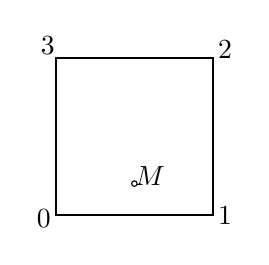
\begin{tikzpicture}
%\draw[step=0.5cm,gray,very thin] (0,0) grid (4,4); %background grid
\draw[thick] (1,1) -- (3,1) -- (3,3) -- (1,3) -- cycle;  
\node[] at (0.85,0.95) {0};
\node[] at (3.15,1) {1};
\node[] at (3.15,3.1) {2};
\node[] at (0.9,3.15) {3};
\node[] at (2.2,1.5) {$M$};
\draw (2.,1.4) circle (1pt);
\end{tikzpicture}\\
\end{center}


%..................................................
\paragraph{An intermediate case} We make the following assumption that the lateral sides of the  
element are vertical while the bottom and top are not necessarily horizontal:

\begin{center}
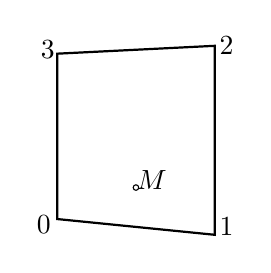
\begin{tikzpicture}
%\draw[step=0.5cm,gray,very thin] (0,0) grid (4,4); %background grid
\draw[thick] (1,1) -- (3,0.8) -- (3,3.2) -- (1,3.1) -- cycle;  
\node[] at (0.83,0.93) {0};
\node[] at (3.15,0.9) {1};
\node[] at (3.15,3.2) {2};
\node[] at (0.88,3.15) {3};
\node[] at (2.2,1.5) {$M$};
\draw (2.,1.4) circle (1pt);
\end{tikzpicture}\\
\end{center}

\noindent Because the sides are verical then if $x_0 \leq x_M \leq x_2$ then 
\[
r_M = \frac{2}{x_2-x_0}(x_M-x_0) -1 
\]
Then, if $M$ is inside the element then its $y$ coordinate is given by
\[
y_M = \sum_i \bN_i(r_M,s_M) y_i
\]
where $\bN_i$ are the four $Q_1$ basis functions associated to the vertices.
Assuming we know $r_M$ then we can solve for $s_M$:
\begin{eqnarray}
y_M &=&  
\frac{1}{4}(1-r_M)(1-s_M) y_0+
\frac{1}{4}(1+r_M)(1-s_M) y_1+
\frac{1}{4}(1+r_M)(1+s_M) y_2+
\frac{1}{4}(1-r_M)(1+s_M) y_3 \nn\\
&=& 
\frac{1}{4} \left[
(1-r)y_0+(1+r)y_1+(1+r)y_2+(1-r)y_3 +s_M [ -(1-r)y_0 - (1+r)y_1+(1+r)y_2+(1-r)y_3  ] 
\right] \nn 
\end{eqnarray}
or, 
\[
s_M = \frac{ 4y_M - [(1-r_M)y_0+(1+r_M)y_1+(1+r_M)y_2+(1-r_M)y_3]  }{ -(1-r_M)y_0 -(1+r_M)y_1+(1+r_M)y_2+(1-r_M)y_3 } 
\]
If the obtained value is in $[-1,1]$ then the point $M$ is in the element.
Verification: when $y_1=y_0$ and $y_2=y_3$ then 
\begin{eqnarray}
s_M 
&=& \frac{4 y_M - [(1-r_M)y_0+(1+r_M)y_0+(1+r_M)y_3+(1-r_M)y_3]  }{ -(1-r_M)y_0 - (1+r_M)y_0+(1+r_M)y_3+(1-r_M)y_3 } \nn\\
&=& \frac{4 y_M - [ 2 y_0 + 2 y_3]  }{ -2 y_0 + 2 y_3    }  \nn\\
&=& \frac{1}{y_3-y_0} [2 y_M - (  y_0 +  y_3) ] \nn\\ 
&=& \frac{1}{y_3-y_0} [2 y_M -  2 y_0 +y_0 -  y_3)  ] \nn\\ 
&=& \frac{2}{y_3-y_0} (y_M - y_0) - 1 
\end{eqnarray}
which is the expression that corresponds to a rectangular element as seen previously.

%..................................................
\paragraph{A generic quadrilateral}

We wish to arrive at a single algorithm which is applicable to all quadrilaterals and we now focus  
on an irregular quadrilateral (no face is parallel to the axis of the coordinate system). 

\begin{center}
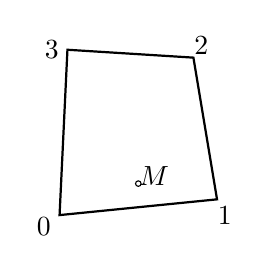
\begin{tikzpicture}
%\draw[step=0.5cm,gray,very thin] (0,0) grid (4,4); %background grid
\draw[thick] (1,1) -- (3,1.2) -- (2.7,3) -- (1.1,3.1) -- cycle;  
\node[] at (0.8,0.85) {0};
\node[] at (3.1,1) {1};
\node[] at (2.8,3.15) {2};
\node[] at (0.9,3.1) {3};
\node[] at (2.2,1.5) {$M$};
\draw (2.,1.4) circle (1pt);
\end{tikzpicture}\\
\end{center}

\noindent Several rather simple options exist:
\begin{itemize}
\item we could subdivide the quadrilateral into two triangles and check whether point $M$ is inside any of them (as it turns out, this problem is rather straightforward for triangles. Simply google it.)
\item We could check that point $M$ is always on the left side of segments $0\rightarrow 1$, $1\rightarrow 2$, $2\rightarrow 3$, $3\rightarrow 0$.
\item ...  
\end{itemize}

Any of these approaches will work although some might be faster than others. 
In three-dimensions all will however become 
cumbersome to implement and might not even work at all. 
Fortunately, there is an elegant way to answer the question, as 
detailed in the following subsection, which works both in 2D and 3D.

%-------------------------------------------
\subsubsection{Three-dimensional space}

If point $M$ is inside the quadrilateral, there exist a set of reduced 
coordinates $r,s,t\in[-1:1]^3$ such that 

\[
\sum_{i=1}^4 \bN_i(r_M,s_M,t_M) x_i = x_M
\quad\quad\quad
\sum_{i=1}^4 \bN_i(r_M,s_M,t_M) y_i = y_M
\quad\quad\quad
\sum_{i=1}^4 \bN_i(r_M,s_M,t_M) z_i = z_M
\]
This can be cast as a system of three equations and three unknowns. 
Unfortunately, each basis function $\bN_i$ 
contains a term $rst$ (as well as $rs$, $rt$, and $st$) 
so that it is not a linear system.
We must then use an iterative technique: the algorithm starts with 
a guess for values $r_M,s_M,t_M$ and 
improves on their value iteration after iteration. 
In what follows the subscript $M$ is dropped from $r,s,t$.

The classical way of solving nonlinear systems of equations is Newton's method. 
\index{general}{Newton's method}
We can rewrite the equations above as ${\bm F}(r,s,t)=0$:
\begin{eqnarray}
\sum_{i=1}^8 \bN_i(r,s,t) x_i - x_M&=&0 \nonumber\\
\sum_{i=1}^8 \bN_i(r,s,t) y_i - y_M&=&0 \nonumber\\
\sum_{i=1}^8 \bN_i(r,s,t) z_i - z_M&=&0
\end{eqnarray}
or,
\begin{eqnarray}
F_r(r,s,t)&=&0 \nonumber\\
F_s(r,s,t)&=&0 \nonumber\\
F_t(r,s,t)&=&0 \nonumber
\end{eqnarray}
so that we now have to find the zeroes of continuously differentiable 
functions ${\bm F}:\mathbb{R} \rightarrow \mathbb{R}$.
The recursion is simply:
\[
\left(
\begin{array}{c}
r_{k+1} \\s_{k+1} \\ t_{k+1}
\end{array}
\right)
=
\left(
\begin{array}{c}
r_{k} \\s_{k} \\ t_{k}
\end{array}
\right)
- J_F(r_k,s_k,t_k) ^{-1} 
\left(
\begin{array}{c}
F_r(r_k,s_k,t_k) \\
F_s(r_k,s_k,t_k)\\
F_t(r_k,s_k,t_k)
\end{array}
\right)
\]
where $J$ the Jacobian matrix:
\begin{eqnarray}
J_F(r_k,s_k,t_k)
&=&
\left(
\begin{array}{ccc}
\frac{\partial F_r}{\partial r}(r_k,s_k,t_k) & \frac{\partial F_r}{\partial s}(r_k,s_k,t_k) & \frac{\partial F_r}{\partial t}(r_k,s_k,t_k) \\\\
\frac{\partial F_s}{\partial r}(r_k,s_k,t_k) & \frac{\partial F_s}{\partial s}(r_k,s_k,t_k) & \frac{\partial F_s}{\partial t}(r_k,s_k,t_k) \\\\
\frac{\partial F_t}{\partial r}(r_k,s_k,t_k) & \frac{\partial F_t}{\partial s}(r_k,s_k,t_k) & \frac{\partial F_t}{\partial t}(r_k,s_k,t_k) 
\end{array}
\right) \nonumber\\
&=&
\left(
\begin{array}{ccc}
\sum\limits_{i=1}^8 \frac{\partial \bN_i}{\partial r}(r_k,s_k,t_k) x_i &
\sum\limits_{i=1}^8 \frac{\partial \bN_i}{\partial s}(r_k,s_k,t_k) x_i &
\sum\limits_{i=1}^8 \frac{\partial \bN_i}{\partial t}(r_k,s_k,t_k) x_i \\
\sum\limits_{i=1}^8 \frac{\partial \bN_i}{\partial r}(r_k,s_k,t_k) y_i &
\sum\limits_{i=1}^8 \frac{\partial \bN_i}{\partial s}(r_k,s_k,t_k) y_i &
\sum\limits_{i=1}^8 \frac{\partial \bN_i}{\partial t}(r_k,s_k,t_k) y_i \\
\sum\limits_{i=1}^8 \frac{\partial \bN_i}{\partial r}(r_k,s_k,t_k) z_i &
\sum\limits_{i=1}^8 \frac{\partial \bN_i}{\partial s}(r_k,s_k,t_k) z_i &
\sum\limits_{i=1}^8 \frac{\partial \bN_i}{\partial t}(r_k,s_k,t_k) z_i 
\end{array}
\right) \nonumber 
\end{eqnarray}
In practice, we solve the following system:
\[
J_F(r_k,s_k,t_k) 
\left[  
\left(
\begin{array}{c}
r_{k+1} \\s_{k+1} \\ t_{k+1}
\end{array}
\right)
-
\left(
\begin{array}{c}
r_{k} \\s_{k} \\ t_{k}
\end{array}
\right)
\right]=-
\left(
\begin{array}{c}
F_r(r_k,s_k,t_k) \\
F_s(r_k,s_k,t_k)\\
F_t(r_k,s_k,t_k)
\end{array}
\right)
\]
Finally, the algorithm goes as follows:
\begin{itemize}
\item set guess values for $r,s,t$ (typically 0)
\item loop over k=0,...
\item Compute rhs= $-{\bm F}(r_k,s_k,t_k)$ 
\item Compute matrix $J_F(r_k,s_k,t_k)$
\item solve system for $(dr_k,ds_k,dt_k)$
\item update $r_{k+1}=r_k+dr_k$, $s_{k+1}=s_k+ds_k$, $t_{k+1}=t_k+dt_k$ 
\item stop iterations when $(dr_k,ds_k,dt_k)$ is small
\item if $r_k,s_k,t_k\in[-1,1]^3$ then $M$ is inside.
\end{itemize}
This method converges quickly but involves iterations, and multiple 
solves of $3\times 3$ systems which, when carried out for each marker 
and at each time step can prove to be expensive. 
A simple modification can be added to the above algorithm: 
iterations should be carried out {\it only}
when the point $M$ is inside of a cuboid of 
size $[\min\limits_i{x_i}:\max\limits_i{x_i}]\times[\min\limits_i{y_i}:\max\limits_i{y_i} ]
\times[\min\limits_i{z_i}:\max\limits_i{z_i}]$ where the sums run over the vertices of the element. 
In 2D this translates as follows: only carry out Newton iterations when $M$ is inside the red rectangle!
\begin{center}
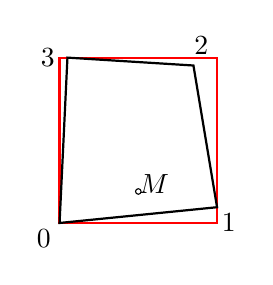
\begin{tikzpicture}
%\draw[step=0.5cm,gray,very thin] (0,0) grid (4,4); %background grid
\draw[thick,red] (1,1) -- (3,1) -- (3,3.1) -- (1,3.1) -- cycle;  
\draw[thick] (1,1) -- (3,1.2) -- (2.7,3) -- (1.1,3.1) -- cycle;  
\node[] at (0.8,0.8) {0};
\node[] at (3.15,1) {1};
\node[] at (2.8,3.25) {2};
\node[] at (0.85,3.1) {3};
\node[] at (2.2,1.5) {$M$};
\draw (2.,1.4) circle (1pt);
\end{tikzpicture}\\
\end{center}

Note that the algorithm above extends to high degree elements 
such as $Q_2$ and higher, even with curved sides.
As shown in the 2D case if the element is a cuboid or 
if all its lateral faces are vertical then one can 
compute the reduced coordinates without using an iterative method.


%-----------------------------------------------------
\subsubsection{Three-dimensional space - special case}

We assume that the mesh is such that the cross section of all $Q_1$ elements 
is a rectangle in the $xy$-plane. 

Let $(x,y,z)$ be a point inside the element. 
The global coordinates $x,y,z$ are obtained from the 
reduced coordinates $r,s,t$ via the basis the basis functions:
\begin{eqnarray}
x=\sum_{i=1}^8 \bN_i (r,s,t) x_i \qquad 
y=\sum_{i=1}^8 \bN_i (r,s,t) y_i  \qquad 
z=\sum_{i=1}^8 \bN_i (r,s,t) z_i \label{xyz}
\end{eqnarray}
Let 
\begin{eqnarray}
{\vec v}_1 &=& (+1,+1,+1,+1,+1,+1,+1,+1) \nn\\
{\vec v}_2 &=& (-1,+1,+1,-1,-1,+1,+1,-1) \nn\\
{\vec v}_3 &=& (-1,-1,+1,+1,-1,-1,+1,+1) \nn\\
{\vec v}_4 &=& (-1,-1,-1,-1,+1,+1,+1,+1) \nn\\
{\vec v}_5 &=& (+1,-1,+1,-1,+1,-1,+1,-1) \nn\\
{\vec v}_6 &=& (+1,-1,-1,+1,-1,+1,+1,-1) \nn\\
{\vec v}_7 &=& (+1,+1,-1,-1,-1,-1,+1,+1) \nn
\end{eqnarray}
and 
\begin{eqnarray}
{\vec x} &=& (x_1,x_2,x_3,x_4,x_5,x_6,x_7,x_8) \nn\\
{\vec y} &=& (y_1,y_2,y_3,y_4,y_5,y_6,y_7,y_8) \nn\\
{\vec z} &=& (z_1,z_2,z_3,z_4,z_5,z_6,z_7,z_8) \nn
\end{eqnarray}
then Eqs.~\eqref{xyz} can also be written
\begin{eqnarray}
x&=&\frac{1}{8} \left( {\vec v}_1 + r  {\vec v}_2 + s  {\vec v}_3 + t  {\vec v}_4 
                 + rs  {\vec v}_5 + rt {\vec v}_6 + st {\vec v}_7 \right) \cdot {\vec x} \nn\\ 
y&=&\frac{1}{8} \left( {\vec v}_1 + r  {\vec v}_2 + s  {\vec v}_3 + t  {\vec v}_4 
                 + rs  {\vec v}_5 + rt {\vec v}_6 + st {\vec v}_7 \right) \cdot {\vec y} \nn\\
z&=&\frac{1}{8} \left( {\vec v}_1 + r  {\vec v}_2 + s  {\vec v}_3 + t  {\vec v}_4 
                 + rs  {\vec v}_5 + rt {\vec v}_6 + st {\vec v}_7 \right) \cdot {\vec z} \label{zzz}
\end{eqnarray}
If the element has a rectangular cross-section $s_x \times s_y$ then 
\begin{eqnarray}
{\vec x} &=& (x_0,x_0+s_x,x_0+s_x,x_0,x_0,x_0+s_x,x_0+s_x,x_0) \nn\\
{\vec y} &=& (y_0,y_0,y_0+s_y,y_0+s_y,y_0,y_0,y_0+s_y,y_0+s_y) \nn
\end{eqnarray}
which yields
\begin{eqnarray}
r&=& 2\frac{x-x_0}{s_x}-1  \nn\\
s&=& 2\frac{y-y_0}{s_y}-1  \nn
\end{eqnarray}
Since the local coordinates $r$ and $s$ can be easily computed, one can use Eq.~\eqref{zzz} to obtain $t$:
\[
t=\frac{8z - ({\vec v}_1 + r {\vec v}_2 + s {\vec v}_3 + rs  {\vec v}_5 ) \cdot {\vec z}} 
{ ({\vec v}_4  + r  {\vec v}_6 + s  {\vec v}_7)  \cdot {\vec z} }
\]







 
 %-------------------------------
\newpage %-----------------------------------------------------------------------------------------
\section{Static condensation} \input{static_condensation} %-------------------------------------
\newpage %-----------------------------------------------------------------------------------------
\section{Measuring incompressibility \label{ss_incomp}} 
The velocity divergence error integrated over the whole element is given by
\begin{equation}
e_{div}= \int_\Omega (\vec\nabla\cdot \vec v^h - \underbrace{\vec\nabla\cdot \vec v}_{=0}  ) \; d\Omega
= \int_\Omega (\vec\nabla\cdot \vec v^h) \; d\Omega
\end{equation}
where $\Gamma_e$ is the boundary of element $e$ and $\vec{n}$ is the unit 
outward normal of $\Gamma_e$.

Furthermore, one can show that \cite{dobo04}:
\[
e_{div} = \int_{\Gamma_e} \vec{v}^h\cdot\vec{n} \;  d\Gamma
\]
The reason is as follows and is called the divergence 
theorem\footnote{\url{https://en.wikipedia.org/wiki/Divergence_theorem}}:
suppose a volume $V$ subset of $\mathbb{R}^d$ which is compact
and has a piecewise smooth boundary $S$, and if $\vec F$ is
a continuously differentiable vector field then
\[
\int_V ( \vec\nabla\cdot\vec F)\; dV = \int_S (\vec F \cdot \vec n)\; dS
\]
The left side is a volume integral while the right side is a surface integral.
Note that sometimes the notation $d\vec S = \vec n \; dS $ is used so that 
$\vec F \cdot \vec n \; dS = \vec F \cdot d\vec S$.

The average velocity divergence over an element can be defined as 
\[
<\vec \nabla \cdot \vec v>_e 
= \frac{1}{V_e} \int_{\Omega_e}  (\vec\nabla\cdot\vec v) \; d\Omega
= \frac{1}{V_e} \int_{\Gamma_e} \vec{v}\cdot\vec{n} \; d\Gamma
\]
Note that for elements using discontinuous pressures we shall 
recover a zero divergence element per element (local mass conservation)
while for continuous pressure elements the mass conservation 
is guaranteed only globally (i.e. over the whole domain), see section 3.13.2 of \cite{grsa}.

Note that one could instead compute $<|\vec\nabla\cdot \vec v|>_e$. Either volume or 
surface integral can be computed by means of an appropriate Gauss-Legendre quadrature algorithm.



 %------------------------
\newpage %-----------------------------------------------------------------------------------------
\section{Periodic boundary conditions\label{ss_periodic}}\input{periodic} %---------------------
\newpage %-----------------------------------------------------------------------------------------
\section{Removing rotational nullspace\label{ss_nullspace}} \input{nullspace} %-----------------
\newpage %-----------------------------------------------------------------------------------------
\section{Picard and Newton \label{ss_nonlinear}} \index{general}{Nonlinear PDE} 
\index{general}{Picard Iterations} 
\index{general}{Relaxation}

\todo[inline]{explain why our eqs are nonlinear}

\Literature Quasi Newton methods \cite{ensb81}

%--------------------------------
\subsubsection{Picard iterations} \label{ss:picard}

Let us consider the following system of nonlinear algebraic equations:
\[
\mathbb{A}(\vec X) \cdot \vec X = \vec b(\vec X)
\]
Both matrix and right hand side depend on the solution vector $\vec X$.

For many mildly nonlinear problems, a simple successive substitution 
iteration scheme (also called Picard method) will converge to the solution
and it is given by the simple relationship:
\[
\mathbb{A}(\vec X^n) \cdot \vec X^{n+1} = \vec b(\vec X^n)
\]
where $n$ is the iteration number. 
It is easy to implement:
\begin{enumerate}
\item guess $\vec X^0$ or use the solution from previous time step
\item compute $\mathbb{A}$ and $\vec b$ with current solution vector $\vec X^{old}$
\item solve system, obtain $T^{new}$
\item check for convergence (are $\vec X^{old}$ and $\vec X^{new}$ close enough?)
\item $\vec X^{old} \leftarrow \vec X^{new}$
\item go back to 2.
\end{enumerate}

There are various ways to test whether iterations have converged. The simplest
one is to look at $\norm{\vec X^{old}-\vec X^{new} }$ (in the $L_1$, $L_2$ or maximum norm)
and assess whether this term is smaller than a given tolerance $\epsilon$. 
However this approach poses a problem: in geodynamics, if two consecutively obtained 
temperatures do not change by more than a thousandth of a Kelvin (say $\epsilon=10^{-3}$K )
we could consider that iterations have converged but looking now at velocities which 
are of the order of a cm/year (i.e. $\sim 3\cdot 10^{-11}$m/s) we would need a tolerance 
probably less than $10^{-13}$m/s. We see that using absolute values for a convergence 
criterion is a potentially dangerous affair, which is why one uses a relative 
formulation (thereby making $\epsilon$ a dimensionless parameter):
\[
\frac{\norm{\vec X^{old}-\vec X^{new}}}{\norm{\vec X^{new}}} < \epsilon
\]
Another convergence criterion is proposed by Reddy (section 3.7.2) \cite{reddybook2}:
\[
\left(
\frac{ (\vec X^{old}-\vec X^{new})\cdot(\vec X^{old}-\vec X^{new} ) }{ X^{new}\cdot X^{new}  } 
\right)^{1/2} < \epsilon
\]
Yet another convergence criterion is used in \cite{thie11}: the means $<\vec X^{old}>$, $<\vec X^{new}>$
as well as the variances $\sigma^{old}$ and $\sigma^{new}$ are computed, followed by the 
correlation factor $R$:
\[
R= \frac{ <  (\vec X^{old}-<\vec X^{old}>)\cdot( \vec X^{new}-<\vec X^{new}> )>  }{\sqrt{\sigma^{old}\sigma^{new}}}
\]
Since the correlation is normalised, it takes values between 0
(very dissimilar velocity fields) and 1 (very similar fields). The
following convergence criterion is then used: $1-R < \epsilon$.

\todo[inline]{write about nonlinear residual}


Note that in some instances and improvement in convergence rate can be obtained by use of a 
relaxation formula where one first solves
\[
\mathbb{A}(\vec X^n) \cdot \vec X^{\star} = \vec b(\vec X^n)
\]
and then updates $\vec X^n$ as follows:
\[
\vec X^n = \gamma \vec X^n + (1-\gamma) \vec X^\star 
\quad\quad\quad
0 < \gamma \leq 1
\]
When $\gamma=1$ we recover the standard Picard iterations formula above.

%------------------------------------------
\subsection{Defect correction formulation}
\index{general}{Defect Correction Formulation}

Work in progress. 

We start from the system to solve:
\[
{\bm A}(\vec X) \cdot \vec X = \vec b(\vec X)
\]
with the associated residual vector $\vec F$ 
\[
\vec F(\vec X) = {\bm A}(\vec X) \cdot \vec X - \vec b(\vec X)
\]
The Newton-Raphson algorithm consists of two steps:
\begin{enumerate}
\item solve $\bm J_k \cdot \delta \vec X_k = -\vec F(\vec X_k)$, or in the 
case of the incompressible Stokes equation FEM system:
\[
\left(
\begin{array}{cc}
\bm J^{{\cal V}{\cal V}}_k & \bm J^{{\cal V}{\cal P}}_k \\
\bm J^{{\cal P}{\cal V}}_k & 0
\end{array}
\right)
\cdot
\left(
\begin{array}{c}
\delta \vec {\cal V}_k \\ \delta \vec {\cal P}_k
\end{array}
\right)
=
\left(
\begin{array}{c}
- \vec F_k^{\cal V} \\ -\vec F_k^{\cal P}
\end{array}
\right)
\]

\item update $\vec X_{k+1} = \vec X_k + \alpha_k \delta \vec X_k$
\end{enumerate}
The defect correction Picard approach consists of neglecting the derivative terms present 
in the $J$ terms (Eqs. 16,17,18 of \cite{frbt19}) so that 
\[
\bm J^{{\cal V}{\cal V}}_k \simeq \K_k 
\quad\quad
\bm J^{{\cal V}{\cal P}}_k \simeq \G 
\quad\quad
\bm J^{{\cal P}{\cal V}}_k \simeq \G^T
\]
and step 1 of the above iterations become:
\[
\left(
\begin{array}{cc}
\K_k & \G \\ \G^T & 0
\end{array}
\right)
\cdot
\left(
\begin{array}{c}
\delta \vec {\cal V}_k \\ \delta \vec {\cal P}_k
\end{array}
\right)
=
\left(
\begin{array}{c}
- \vec F_k^{\cal V} \\ -\vec F_k^{\cal P}
\end{array}
\right)
\]


\mscthesis: implement a simple Newton solver and apply it to a few nonlinear 
benchmarks. \index{general}{MSc Thesis} 

\vspace{1cm}

\todo[inline]{explain picard, defect picard, Newton, line search, ....}


\begin{itemize}
\item \fullcite{erka81}
\item \fullcite{ensb81}
\item \fullcite{knke04}
\item \fullcite{yiha10}
\item \fullcite{sara16}
\item \fullcite{frbt19}
\item \fullcite{russ20}
\end{itemize}

 %----------------------------
\newpage %-----------------------------------------------------------------------------------------
\section{Parallel or not?} \label{sec:parallel} \input{parallel} %------------------------------
\newpage %-----------------------------------------------------------------------------------------
\section{Stream function} \label{sec:streamfunction} \index{general}{Stream Function}
\begin{flushright} {\tiny {\color{gray} streamfunction.tex}} \end{flushright}

\Literature 
\textcite{scja81} (1981),
\textcite{chyu84} (1984),
\textcite{chri84} (1984),
\textcite{hayu94} (1994),
\textcite{olwh97} (1997),
\textcite{giju98} (1998),
\textcite{vanv08} (2008),
\textcite{vanj11} (2011).

\vspace{0.5cm}

The Stream function (commonly denoted by $\Phi$ or $\Psi$) approach is a useful approach in 
fluid dynamics as it 
can provide relatively quick solutions to 2D incompressible flow problems.
Using a stream function
formulation is numerically convenient because velocity information is contained in a single scalar equation
and pressure vanishes from the solution process.
The stream function is a function of coordinates and time of an inviscid liquid.
It allows to determine the components of velocity by differentiating the stream function 
with respect to the space coordinates. 
A family of curves $\Psi = constant$ represent {\color{olive} streamlines}, i.e. 
the stream function remains constant along a streamline. 
Although also valid in 3D, this approach is mostly used in 2D because of its 
relative simplicity.

%............................................
\subsubsection{In Cartesian coordinates - 2D}

In two dimensions the velocity is obtained as follows:
\begin{equation}
{\vec \upnu} = (u,v) = \left( \frac{\partial \Psi}{\partial y},-\frac{\partial \Psi}{\partial x} \right) 
\end{equation}
Provided the function $\Psi$ is a smooth enough function, 
this automatically insures that the flow is incompressible:
\begin{equation}
{\vec \nabla}\cdot {\vec \upnu} = 
\frac{\partial u}{\partial x} + \frac{\partial v}{\partial y}
=
\frac{\partial^2 \Psi}{\partial xy} - \frac{\partial^2 \Psi}{\partial xy} =0 
\end{equation}
Assuming constant viscosity, the Stokes equation writes:
\begin{equation}
-{\vec \nabla}p + \eta \Delta {\vec \upnu} + \rho {\vec g} = \vec{0}
\end{equation}
Let us introduce the vector $\vec{W}=(W_x,W_y)$ for convenience such that in each dimension:
\begin{eqnarray}
W_x&=&-\frac{\partial p}{\partial x} 
+ \eta\left( \frac{\partial^2 u}{\partial x^2} + \frac{\partial^2 u}{\partial x^y} \right) \\
W_y&=&-\frac{\partial p}{\partial y} 
+ \eta \left(\frac{\partial^2 v}{\partial x^2} + \frac{\partial^2 v}{\partial x^y} \right) 
\end{eqnarray}
Taking the curl of the vector ${\vec{W}}$ and only considering the component 
perpendicular to the $xy$-plane:
\begin{equation}
\frac{\partial W_y}{\partial x} - \frac{\partial W_x}{\partial y}  = 
-\frac{\partial \rho g_y}{\partial x} + \frac{\partial \rho g_x}{\partial y}   
\end{equation}
The advantage of this approach is that the pressure terms cancel out 
(the curl of a gradient is always zero\footnote{\url{https://mathinsight.org/curl_gradient_zero}}), 
so that:
\begin{equation}
\frac{\partial}{\partial x}\eta\left( \frac{\partial^2 v}{\partial x^2} + \frac{\partial^2 v}{\partial x^y}  \right) 
- \frac{\partial }{\partial y} \eta \left( \frac{\partial^2 u}{\partial x^2} + \frac{\partial^2 u}{\partial x^y} \right) = 
-\frac{\partial \rho g_y}{\partial x} + \frac{\partial \rho g_x}{\partial y}   
\end{equation}
and then replacing $u,v$ by the their stream function derivatives yields (for a constant viscosity):
\begin{equation}
\eta \left(\frac{\partial^4 \Psi}{\partial x^4} + 
\frac{\partial^4 \Psi}{\partial y^4} + 
2\frac{\partial^4 \Psi}{\partial x^2y^2} \right)
=
-\frac{\partial \rho g_y}{\partial x} + \frac{\partial \rho g_x}{\partial y}   
\end{equation}
or, 
\begin{equation}
\eta {\vec \nabla}^4 \Psi 
=
\left(\frac{\partial^2 }{\partial x^2} + \frac{\partial^2 }{\partial y^2} \right) 
\left(\frac{\partial^2 }{\partial x^2} + \frac{\partial^2 }{\partial y^2} \right) \Psi
=
-\frac{\partial \rho g_y}{\partial x} + \frac{\partial \rho g_x}{\partial y}   
\label{eq:sf1}
\end{equation}
Note that $\vec\nabla^2 \vec\nabla^2 = \vec\nabla^4 $ is known as the {\color{olive}Biharmonic operator}.
\index{general}{Biharmonic Operator} 
These equations are also to be found in the geodynamics literature, 
see \textcite[eq. 1.43]{tack10} or \textcite[p 70-71]{gery10}.

In the presence of temperature variations and multiple compositions, 
\textcite{trlb20} (2020)  use the  following nondimensional equation:
\[
\left(
\frac{\partial^2 }{\partial x^2} - 
\frac{\partial^2 }{\partial y^2}  
\right)
\left[ \eta
\left(
\frac{\partial^2 \Psi}{\partial x^2} - 
\frac{\partial^2 \Psi}{\partial y^2}  
\right)
\right]
+4
\frac{\partial^2 }{\partial xy} 
\left[
\eta 
\frac{\partial^2 \Psi}{\partial xy} 
\right]
=
Ra_T \frac{\partial T}{\partial x}-
Ra_C \frac{\partial C}{\partial x}
\]
\todo[inline]{check/rederive this formula!}

%........................................
%\subsubsection{In Cylindrical coordinates}

%TODO

%VERIFY THOSE! minus signs ?
%\[
%\upnu_r=\frac{1}{r}\frac{\partial \Phi}{\partial \theta} 
%\]
%\[
%\upnu_\theta=-\frac{\partial \Phi}{\partial r} 
%\]


%............................................
\subsubsection{In Cartesian coordinates - 3D}

See for example \textcite{hous90} (1990) and refs therein.


 %-------------------
\newpage %-----------------------------------------------------------------------------------------
\section{Corner flow} \label{sec:cornerflow} \input{cornerflow} %-------------------------------
\newpage %-----------------------------------------------------------------------------------------
\section{Surface processes \label{sec:surfaceprocesses}} \begin{flushright} {\tiny {\color{gray} surfaceprocesses.tex}} \end{flushright}

%.......................................................................
\subsubsection{In 1D - simple nonlinear diffusion a la Burov \& Cloetingh (1997)}

This approach comes from \textcite{bucl97} (1997).
The tectonic-scale transport equations describe long term changes
in topography $h(x,y,t)$ as a result of simultaneous short- and long-range
mass transport processes \cite{befh92,kobe94}.

The short-range surface processes are represented by cumulative effects of hillslope 
processes (soil creep, rainsplash, slides) that remove material from uplifted areas 
down to the valleys. 
It is then assumed that the horizontal material flux $\vec{q}_s$ is related to 
local slope $\vec\nabla h$ by $\vec{q}_s=-K_s \vec{\nabla}h$ 
where $K_s$ is the effective diffusivity. Assumption of conservation of mass 
volume leads to the linear diffusion equation for erosion:
\[
\frac{\partial h}{\partial t} = K_s \Delta h
\]
This equation can be solved with constant-elevation (fixed $h$ value)
boundary conditions simulating local base levels of erosion. 

Note that is practice the coefficient $K_s$ might depend on slope and curvature, 
i.e.
\[
\frac{\partial h}{\partial t} = K_s(x,y,h,\vec\nabla h)\Delta h
\]
Following \cite{goss76}, Burov \& Cloetingh use an empirical non linear 
expression $K_s=k_s(x) (\vec\nabla h)^n$. 




%...........................................................
\subsubsection{In 1D - not so simple, a la Andr\`es-Martinez \etal (2019)}

This approach comes from \textcite{anpa19} (2019). 
The change in surface elevation rate due to surface processes is equal
to the divergence of the sediment flux 
(assuming there is no density difference between the bedrock and
sediment and ignoring the effects of compaction):
\[
\frac{\partial h}{\partial t} = -\frac{\partial q_s}{\partial x}
\]
where $h$ is the topography, $t$ is the time, $q_s$ represents the sediment flux, 
and $x$ is the horizontal coordinate. 

The next step consists in a formulation for the sediment flux. Still following \cite{anpa19}, 
in the subaerial environment, it is possible to define the sediment transport 
flux $q_s$ in terms of the water flux $q_w$ as
\[
q_s=-(K+c q_w^n) \frac{\partial h}{\partial x}
\]
where $K$ is the slope diffusivity, $c$ is the transport coefficient, 
and $n \geq 1$ is the power law that defines the type
of relationship between the sediment transport and the water flux 
(Simpson \& Schlunegger, 2003; Smith \& Bretherton, 1972).
\todo[inline]{get these papers}
This model accounts for hillslope diffusion processes where the topography will tend to
a dispersive diffusion (Culling, 1960) and fluvial transport processes that result in concentrative diffusion
due to water run off (Graf, 1984). For a simple parameterization we choose a linear relationship between
sediment transport and water flux $(n=1)$.

The water flux can be related to the water discharge/effective rainfall $\alpha$ as
\[
\frac{\partial}{\partial x} (\vec{n} q_w) = -\alpha
\]
where $\vec n$ is a unit vector directed down the surface gradient (Smith \& Bretherton, 1972). 
By assuming a constant $\alpha$ and integrating equation (12) over the surface in the downstream direction, we obtain

\[
q_w = \alpha x_d
\]
where $x_d$ is the downstream distance from the drainage divide. By substituting equations (11) and
(13) into (10) we obtain the 1-D sediment mass conservation equation for combined hillslope and
discharge-dependent fluvial transport
\[
\frac{\partial h}{\partial t} = \frac{\partial}{\partial x} \left( (K+k \alpha x_d) 
\frac{\partial h}{\partial x}   \right)
\]
where the downstream distance $x_d$ is calculated at each time step as the distance from the topographic highs
to the valley floors. Because $q_w$ is dependent on the length of the drainage, the model mimics 1-D landscapes
similar to river profiles in which fluvial processes are dominant.

%...........................................................
\subsubsection{Examples in the literature}

\begin{center}
\includegraphics[width=7cm]{images/surfaceprocesses/fuwf06a}
\includegraphics[width=7cm]{images/surfaceprocesses/fuwf06b}\\
{\captionfont Application to Taiwan. Taken from Fuller \etal (2006) \cite{fuwf06}}
\end{center}


 %-------------
\newpage %-----------------------------------------------------------------------------------------
\section{Geometric multigrid} \input{gmg} %-----------------------------------------------------
\newpage %-----------------------------------------------------------------------------------------
\section{Algebraic multigrid} \input{amg} %-----------------------------------------------------
\newpage %-----------------------------------------------------------------------------------------
\section{Computing depth \label{ss:depth}} \input{computing_depth} %----------------------------
\newpage %-----------------------------------------------------------------------------------------
\section{Imposing boundary conditions \label{ss:howtobc}} 
\begin{flushright} {\tiny {\color{gray} howtobc.tex}} \end{flushright}

Let us consider a quadrilateral element with one degree of freedom per node and let us assume that we are solving the temperature equation. The local matrix and right-hand side vector are given by 
\[
A_{el}(4\times 4) \quad\quad {\text and} \quad\quad B_{el}(4)
\]
Let us assume that we want to impose $\tilde{T}=10$ on the third node (local coordinates numbering). For instance, having built $A_{el}$ and $B_{el}$, the system looks like :
\[
\left(
\begin{array}{cccc}
3 & 1 & 6  & 9 \\
5 & 2 & 2  & 8 \\
7 & 4 & 11 & 2 \\
9 & 6 & 4  & 3
\end{array}
\right)
\left(
\begin{array}{c}
T_1 \\ T_2 \\ T_3 \\ T_4
\end{array}
\right)
=
\left(
\begin{array}{c}
4 \\ 3 \\ 1 \\ 2
\end{array}
\right)
\]

\begin{itemize}

\item \underline{Technique 1:} Penalty approach. Replace the hereabove system by
\[
\left(
\begin{array}{cccc}
3 & 1 & 6  & 9 \\
5 & 2 & 2  & 8 \\
7 & 4 & 11 +  10^{12} & 2 \\
9 & 6 & 4  & 3
\end{array}
\right)
\left(
\begin{array}{c}
T_1 \\ T_2 \\ T_3 \\ T_4
\end{array}
\right)
=
\left(
\begin{array}{c}
4 \\ 3 \\ \tilde{T}\times (11 + 10^{12}) \\ 2
\end{array}
\right)
\]




\item \underline{Technique 2:} One can choose not to solve for $T_3$ anymore, i.e. not to consider it as a degree of freedom, remove the corresponding 
equation and therefore write the linear system as follows:

\begin{eqnarray}
3 T_1 + T_2 + 6 T_3 + 9 T_4 &=& 4 \nn\\
5 T_1 + 2T_2 + 2 T_3 + 8 T_4 &=& 3 \nn\\
7 T_1 + 4T_2 + 11 T_3 + 2 T_4 &=& 1 \nn\\
9 T_1 + 6T_2 + 4 T_3 + 3 T_4 &=& 2\nn
\end{eqnarray}
or, 
\[
3 T_1 + T_2 + \quad  + 9 T_4 = 4 - 6T_3
\]
\[
5 T_1 + 2T_2 + \quad + 8 T_4 = 3 - 2T_3
\]
\[
7 T_1 + 4T_2 + 11T_3 + 2 T_4 = 1 
\]
\[
9 T_1 + 6T_2 + \quad + 3 T_4 = 2 - 4T_3
\]
and in the end:
\[
3 T_1 + T_2 + 9 T_4 = 4 - 6T_3
\]
\[
5 T_1 + 2T_2 + 8 T_4 = 3 - 2T_3
\]
\[
9 T_1 + 6T_2 +  3 T_4 = 2 - 4T_3
\]


\item \underline{Technique 3:} Since we want to impose $T_3=10$, then we can write 
\[
3 T_1 + T_2 + \quad  + 9 T_4 = 4 - 6T_3
\]
\[
5 T_1 + 2T_2 + \quad + 8 T_4 = 3 - 2T_3
\]
\[
0 + 0 + T_3 + 0 = 10
\]
\[
9 T_1 + 6T_2 + \quad + 3 T_4 = 2 - 4T_3
\]
and in matrix form :
\[
\left(
\begin{array}{cccc}
3 & 1 & 0  & 9 \\
5 & 2 & 0  & 8 \\
0 & 0 & 1 & 0 \\
9 & 6 & 0  & 3
\end{array}
\right)
\left(
\begin{array}{c}
T_1 \\ T_2 \\ T_3 \\ T_4
\end{array}
\right)
=
\left(
\begin{array}{c}
4 - A_{13} T_3\\ 3 - A_{23}T_3 \\ 10 \\ 2-A_{43} T_3
\end{array}
\right)
\]

\end{itemize}

The first technique is not a good idea in practice as it introduces very large 
values and will likely derail the solver. The second option is somewhat difficult
to implement as it means that elemental matrix and rhs sizes will change from 
element to element and it therefore requires more book-keeping.
The third technique is the one adopted throughout this document. 

As shown in \textcite{wuxl08} (2008), it is better to replace the 1 on the diagonal 
by the former diagonal term as it reduces the condition number of the matrix. 
The rhs must then be modified accordingly.

\Literature Behr (2004) \cite{behr04}

\todo{ASK DAVE for permission} This is an excerpt of an email sent to me by Dave May in May 2014: 
{\it 
Never ever ever impose bc's using a penalty approach.
For problems with a fixed mesh topology and time dependent Dirichlet domain (e.g. the segment 
of the boundary with Dirichlet bc's 
maybe change size/shape over time - for example with a true stick/slip type interface), it's nice to define the matrix 
with the dimension associated with the mesh+basis and leave all bc's in the operator. 
Leaving the bc's in the operator can be implemented in a manner which still retains the operators symmetry (assuming 
it was symmetric to begin with). This leaves the choice of what to stick on the diagonal. Simply using "1" could 
screw up the spectrum of the matrix and kill the iterative solver performance. A better choice would be to insert 
a diagonal entry closely related to the operator; e.g. something that looks like the diagonal entry 
of $\int 2 \eta \epsilon(u) : \epsilon(v) dV$ (for the discrete stress tensor term). 

Removing Dirichlet bc's entirely for the discrete operator sounds attractive. The code will like the FE theory 
and you will only be solving for variables which are "unknowns" (compared with the above). 
However, introducing a time dependent Dirichlet domain means the matrix must be re-sized, as should its non-zero structure 
be re-allocated. Also, implemented multi-grid is annoying when the Dirichlet entries are removed. In fact, most of  
the code associated with stripping out Diriclet bc's is annoying and ugly. However, removing the bcs ensures symmetry, 
it ensures the discrete operator will have a nice spectrum (c.f. the above option). Also, stripping out bcs usually 
increases overall storage as you have one representation of the discrete vectors given to the solver which will be  
of size (N-n) and in your mesh you will have a repsentation of length N. ``N'' being the total number of dofs in your 
system, ``n'' being the number of Dirichlet constrained dofs in your system. }
 
 %---------------------
\newpage %-----------------------------------------------------------------------------------------
\section{The Geoid} \label{ss:geoid} 
%---------------------------------
\subsubsection{What is the geoid?}
\index{general}{Geoid}


There is an infinity of equipotential surfaces of the gravitational potential $U$.
However, there is a particular surface on the Earth that is "easy" to locate: 
the mean sea level. This is a somewhat arbitrary choice  
but it makes sense because the oceans are made of water (!): 
the surface of a fluid in equilibrium must follow an equipotential.

\begin{center}
\includegraphics[width=6cm]{images/geoid/geoid1}
\end{center}

The geoid is usually defined in two ways:
\begin{itemize}
\item it is the particular equipotential surface that coincides with the mean sea level
 (easy to define in the oceans -assuming no currents, waves,... - but harder on land since 
it is not the topographic surface).
\item A gravitational equipotential surface. This means that everywhere at sea level experiences the same value of gravity potential, so there is no tendency for water to flow downhill since all points in the vicinity have the same value of gravity potential, pointed toward the center of the earth.
\end{itemize}

\begin{center}
\includegraphics[width=13cm]{images/geoid/ww15mgh}\\
{\captionfont Data Max value: 85.4 meters, east of New Guinea. Data Min value:-107.0 meters, south of India. 
This image shows 15'x15' geoid undulations covering the planet Earth 
from the NIMA/GSFC WGS-84 EGM96 15' Geoid Height File. The undulations refer to 
the differences from the WGS-84(G873) reference ellipsoid. 
Map and description from National Geodetic Survey
\footnote{\url{https://www.usna.edu/Users/oceano/pguth/md_help/geology_course/geoid.htm}}
}
\end{center}

From Wikipedia: The geoid surface is irregular, unlike the reference ellipsoid 
(which is a mathematical idealized representation of the physical Earth), but 
is considerably smoother than Earth's physical surface. Although the physical Earth has 
excursions of +8,848 m (Mount Everest) and -11,034 m (Marianas Trench), 
the geoid's deviation from an ellipsoid ranges from +85 m (Iceland) to -106 m (southern India), 
less than 200 \si{metre} total.


\begin{center}
\includegraphics[width=8cm]{images/geoid/Geoid}\\
{\captionfont 1. Ocean
2. Reference ellipsoid
3. Local plumb line
4. Continent
5. Geoid\\
Taken from \url{https://en.wikipedia.org/wiki/Geoid}}
\end{center}


%----------------------------------------
\subsubsection{the (reference) ellipsoid}

First evidence that the Earth is round Erathostene (275-195 B.C.)

First hypothesis that the Earth is flattened at the poles: Newton

First measurement of the Earth's flattening at the poles: Clairaut (1736) and Bouguer (1743)

The shape of the Earth can be mathematically represented as an ellipsoid defined by:
\begin{itemize}
\item Semi-major axis = equatorial radius = $a$
\item Semi-minor axis = polar radius = $c$
\item Flattening (the relationship between equatorial and polar radius): $f = (a-c)/a$
\item Eccentricity: $e^2 =2f-f^2$
\end{itemize}

Many different reference ellipsoids have been defined and are in use.
We define the {\it reference ellipsoid} = the ellipsoid that best fits the geoid.
It is totally arbitrary, but practical. 
The most common reference ellipsoid is the WGS-84 one\footnote{\url{https://confluence.qps.nl/qinsy/latest/en/world-geodetic-system-1984-wgs84-182618391.html}}:

\begin{center}
\includegraphics[width=6cm]{images/geoid/ellipsoid_wgs84}\\
Taken from \url{https://en.wikipedia.org/wiki/Reference_ellipsoid}
\end{center}


Geoid undulations = differences, in meters, between
the geoid reference ellipsoid
(= geoid ``height'').

To clarify:
\begin{itemize}
\item Geoid = the equipotential surface of the Earth's gravity field that
best fits (in a least squares sense) the mean sea level.
The gravitational potential is constant on the geoid (by definition) but 
the gravitational acceleration is not! 

\item Reference Ellipsoid = the ellipsoid that best fits the geoid 
\item Geoid = the (actual) figure of the Earth 
\item Ellipsoid = the (theoretical) shape of the Earth
\end{itemize}



%---------------------------------
\subsubsection{How to compute it?}

From \textcite{lizh16} (2016): ``
The geoid is computed by $\phi/g$, where $\phi$ is the surface gravitational potential anomaly 
and can be solved from the Poisson equation,
$ \nabla^2 \phi = -4\pi {\cal G} \delta\rho$ 
where ${\cal G}$ is the gravitational constant, and $\delta\rho$ 
includes both density variations in the mantle [...]
and those associated with dynamic topographies at the surface and CMB. 
Dynamic topographies are determined from solving [the Stokes] equations 
under free-slip boundary conditions at the surface and CMB.''


%---------------------------------
\subsubsection{Interesting modelling}

\begin{center}
\includegraphics[width=15cm]{images/geoid/mogu96}
{\scriptsize Idealized 2D slab calculations for each viscosity model: geoid and geoid filtered 
to pass only the longest wavelengths ($\sim$ 4000 km).
(a) Cold slab extends to 500 km depth in the upper mantle, 
(b) Slab extends to 750 km so that it is partly supported by the high viscosity lower mantle at 670 km. 
(c) Slab tilted at 45\degree to the vertical extending to the top of the lower mantle. 
Taken from \cite{mogu96}}
\end{center}
 %--------------------------------------------
\newpage %-----------------------------------------------------------------------------------------
\section{The Lyapunov time/exponent, mixing stirring}\label{ss:lyapunov}\index{general}{Lyapunov Time}
\begin{flushright} {\tiny {\color{gray} lyapunov.tex}} \end{flushright}

%from wiki

Simply put, the Lyapunov time is the characteristic timescale on which a dynamical system is chaotic.
 It is defined as the inverse of a system's largest Lyapunov exponent.

The Lyapunov time mirrors the limits of the predictability of the system. By convention, it is defined 
as the time for the distance between nearby trajectories of the system to increase by a factor of $e$. 
However, measures in terms of 2-foldings and 10-foldings are sometimes found, since they correspond to 
the loss of one bit of information or one digit of precision respectively.

The Lyapunov exponent or Lyapunov characteristic exponent of a dynamical system is a quantity 
that characterizes the rate of separation of infinitesimally close trajectories. 
Quantitatively, two trajectories in phase space with initial separation $\delta \mathbf{Z}_0$ 
diverge (provided that the divergence can be treated within the linearized approximation) at a rate given by
\[
|\delta \mathbf{Z} (t)|\approx e^{\lambda t}|\delta \mathbf {Z} _{0}| 
\]
where $\lambda$ is the Lyapunov exponent. 

Measuring the Lyapunov exponent or time (or related quantities) is relevant in the context of mantle stirring. 
On the one hand it is argued that the mantle is convecting and very efficient at mixing resulting in a 
somewhat homogenous composition. On the other hand, there is are modeling studies that suggest that
whole-mantle convection can preserve heterogeneity in the presence of well-mixed mantle. 

%from vazh99
Mixing takes place by the repeated stretching
and folding of interfaces. A measure of the
mixing efficiency is the time evolution of the area of
the mixing surface. Maximum efficiency of mixing
is reached with turbulent mixing behavior where
One can formally show whether mixing is laminar or turbulent by evaluating the Luyaponov exponents $\sigma$ .
These are of the form:
\[
\sigma = \lim_{t\rightarrow \infty} \lim_{X\rightarrow 0} \left[  \frac{1}{t} \ln \left( \frac{X(t)}{X(t=0)} \right)   \right]
\]
where $X(t)$ is the length of this segment at time t.
Non-zero Luyaponov exponents indicate that
stretching is exponential and the larger the exponent,
the more efficient mixing is.
However, the limits in the above equation are difficult to evaluate and the interpretation 
of the 'finite-time' Luyaponov exponent, where both limits are truncated, is difficult to formalize.


Two approaches are taken in the literature when it comes to studying mixing/stirring and/or measuring Lyapunov quantities::

\begin{itemize}
\item using marker advection: in \textcite{vazh99} (1999) the authors use a steady state velocity
pattern obtained for a model of present-day mantle convection. The velocity model is
based on the solution of the Stokes equations in a 3D spherical model with variable rheology.
To study mixing, they release particles in the velocity model and follow 
these by numerical integration. 

\begin{center}
\includegraphics[width=6cm]{images/mixing/vazh99}\\
{\captionfont a) The three particles in this plot were
selected for their relatively regular pattern. 
b) Three other particles that traverse a large portion of the model. These particles feel 
the strong toroidal motion and their paths form corkscrew-like patterns. 
They indicate that certain parts of the model can exhibit strong mixing. 
Taken from \textcite{vazh99} (1999).}
\end{center}

Rather than calculating the exponents explicitly, the authors 
use an approximation to the finite-time,
finite-length Luyaponov exponent by evaluating the distance between two points that are closely spaced
at time $t=0$. For this they compute the advection of a
large number of 10 km long line segments that were
originally at 1500 km depth. The length of these segments is approximated by the distance between the
endpoints and the results are summarized in the following figure:

\begin{center}
\includegraphics[width=7cm]{images/mixing/vazh99b}\\
{\captionfont Length
of the line segment after 4 billion years. Approximately 14,000 line segments were released with 
regular spacing at 1500 km depth. The length of the segment is indicated by the colored symbols 
that are plotted at the initial position. The results indicate that there is a strong
diversity in mixing behavior. In some regions (north Pacific, parts under the Indian/Australian plate) 
stretching is very limited, indicating laminar and consequently inefficient mixing. Regions that 
are under strong toroidal surface motion (western Pacific, Nazca and South
America) show very efficient stretching of up to the maximum length of the diameter of the Earth. 
Taken from \textcite{vazh99} (1999).}
\end{center}


\item twin experiments: \fullcite{becr14} (2014)
\end{itemize}

Talk about configurational entropy \fullcite{gobo02},\fullcite{nake07} (2007), van der Wiel et al.
\fullcite{cakm06} 

Talk about retrodiction (reconstructions of past states of Earth's mantle obtained using present information)
\textcite{cobs15} (2015),
\textcite{cogb18} (2018).

\Literature: 
\textcite{scha94} (1994),
\textcite{schh96} (1996),
\textcite{vazh99} (1999),
\textcite{falt02} (2002),

\textcite{fasa03} (2003),
\textcite{saad11} (2011),

\textcite{sato12} (2012) measure the convective stirring efficiency using two Lagrangian methods: 
the first determines the mixing time associated with
different wavelengths of heterogeneity following the approach of
Ferrachat and Ricard (2001). The second determines the value of
the maximum Finite Time Lyapunov Exponents (FTLE) as de-
scribed in Farnetani and Samuel (2003), and measures the rate at
which heterogeneities are stretched by mantle motions.

Investigating the initial condition
of mantle models using data assimilation. PhD thesis. \textcite{pric16} (2016).

Reconstruction of mantle convection and surface tectonics with (ensemble) Kalman filter:
\fullcite{bocf16} (2016),
\fullcite{bofc18} (2018).

Stirring: \fullcite{gowh06} 

 %------
\newpage %-----------------------------------------------------------------------------------------
\section{Phase transitions}\label{ss:phasetransitions}\input{phasetransitions} %----------------
\newpage %-----------------------------------------------------------------------------------------
\section{Open boundary conditions}\label{ss:openbc}\begin{flushright} {\tiny {\color{gray} openbc.tex}} \end{flushright}
%~~~~~~~~~~~~~~~~~~~~~~~~~~~~~~~~~~~~~~~~~~~~~~~~~~~~~~~~~~~~~~~~~~~~~~~~~~~~~~~~~~~~~~~~~~~~~~~~~~

So-called open boundary conditions have a special meaning in computational geodynamics. 
They usually refer to the boundary conditions on the sides of Cartesian models, 
usually looking at subduction or rifting processes. 

In the literature boundary conditions on the vertical sidewalls are usually 
\begin{itemize}
\item no-slip (no flow at the boundary), 
\item free slip (impermeable); 
\item open to some particular form of through-flow.
\end{itemize}

Free slip is the most commonly used boundary condition while prescribed in- and outflow 
or periodic boundary conditions are also common. (REF?)

Taken from \textcite{chgv12} (2012):
``Open boundaries for which the horizontal in- and outflow are defined by a fully 
internally developed flow, have hardly been used [...]. 
Such open boundaries basically prescribe a hydrostatic pressure condition on 
the boundary preventing the model to collapse while horizontal in and outflow is free, 
in the sense that it is driven by the internal dynamics and the usual condition of 
incompressible flow. 
Among the range of boundary conditions used, open boundaries may fit best to 
real-mantle flow conditions surrounding subduction zones.''

Two examples of the use of such boundary conditions were found in 
the literature: \textcite{qusp10} (2010) and \textcite{chgv12} (212).

We start again from the variational form of the momentum equation, and focus on the term containing 
the full stress tensor ${\bm \sigma}$. 
Let us look at the stress tensor gradient, multiplied by the basis function $\bN$, integrated over the domain:
\begin{eqnarray}
\int_V \bN {\vec \nabla}\cdot {\bm \sigma} \; dV 
&=&\int_V \left[ {\vec \nabla}\cdot(\bN {\bm \sigma}) -{\vec \nabla} \bN \cdot {\bm \sigma}\right] \; dV \nonumber\\
&=& \int_V  {\vec \nabla}\cdot(\bN {\bm \sigma})\;  dV -\int_V  {\vec \nabla}\bN \cdot {\bm \sigma} \; dV
\end{eqnarray}
The right term yields the $\K$ and $\G$ matrices after discretisation, as seen in Section~\ref{XXX}.
Turning to the left term, we then make use of the Green-Gauss divergence 
theorem\footnote{\url{https://en.wikipedia.org/wiki/Divergence_theorem}} which states that for 
a continuously differentiable vector field $\vec{F}$:
\[
\int_V ({\vec \nabla} \cdot {\vec F})\; dV = \int _S {\vec F}\cdot {\vec n} \; dS
\]
so that (applying it now to tensors):
\[
\int_V  {\vec \nabla}\cdot(\bN {\bm \sigma})\;  dV =\int_S  \bN {\bm \sigma} \cdot {\vec n} \;  dS
\]
This right hand side term is responsible for the surface 
boundary conditions and cannot be neglected if one 
wishes to implement stress boundary conditions, 
such as the so-called open boundary conditions. 

Note that in \textcite{lige17} (2017) the authors describe an iterative algorithm that 
allows them to control the actual force applied at the boundary by 
scaling the kinematical boundary conditions

%.................................................................
\subsection{Two-dimensional case - $Q_1 \times P_0$ elements}

On the following figure two elements are represented, one on the 
left boundary, one on the right boundary:
\begin{center}
\includegraphics[width=5cm]{images/openbc/drawing.png}
\end{center}

The prescribed traction on the leftt boundary is
\[
{\vec t}={\bm \sigma}\cdot {\vec n}=
\left(
\begin{array}{cc}
-p_{bc} & 0 \\
0 & -p_{bc}
\end{array}
\right)
\cdot
\left(
\begin{array}{c}
-1 \\ 0
\end{array}
\right)
=
\left(
\begin{array}{c}
p_{bc} \\ 0
\end{array}
\right)
\]
The integral on the side of the element is then 
\[
\int_\Gamma \bN_i {\vec t} \; dS
\]
for $i=1,2,3,4$, which yields the following elemental rhs vector:
\[
\vec{F}_{el}=
\int_{\Gamma_{14}} 
\left(
\begin{array}{c}
\bN_1(x,y) t_x(x,y)\\
\bN_1(x,y) t_y(x,y)\\
\bN_2(x,y) t_x(x,y)\\
\bN_2(x,y) t_y(x,y)\\
\bN_3(x,y) t_x(x,y)\\
\bN_3(x,y) t_y(x,y)\\
\bN_4(x,y) t_x(x,y)\\
\bN_4(x,y) t_y(x,y)
\end{array}
\right)
\; dS
\]
It is worth noting that the integral takes place on the edge $\Gamma_{14}$ 
so that $\bN_2$ and $\bN_3$ are identically zero on this edge
and also $t_y=0$ 
so 
\[
\vec{F}_{el}=
\left(
\begin{array}{c}
\int_{\Gamma_{14}}  \bN_1(x,y) t_x(x,y) dS\\
0 \\
0 \\ 0 \\ 0 \\ 0 \\
\int_{\Gamma_{14}} \bN_4(x,y) t_x(x,y) dS\\
0
\end{array}
\right)
\]
If the traction (applied pressure) is constant over the element, 
then  
\[
\vec{F}_{el}=
t_x
\left(
\begin{array}{c}
\int_{\Gamma_{14}}  \bN_1(x,y)  dS\\
0 \\
0 \\ 0 \\ 0 \\ 0 \\
\int_{\Gamma_{14}} \bN_4(x,y)  dS\\
0
\end{array}
\right)
=
t_x
\left(
\begin{array}{c}
\int_{y_1}^{y_4} \bN_1(x,y) dy\\
0 \\
0 \\ 0 \\ 0 \\ 0 \\
\int_{y_1}^{y_4} \bN_4(x,y) dy\\
0
\end{array}
\right)
=
\frac{t_x h_y}{2}
\left(
\begin{array}{c}
1 \\
0 \\
0 \\ 0 \\ 0 \\ 0 \\
1 \\
0
\end{array}
\right)
\]
where $h_y$ is the height of the element along the segment. 



On the right boundary, we have $\bN_2=0$ and $\bN_3=0$, and since $t_y=0$ then 
the corresponding additional elemental right hand side vector writes:
\[
\vec{F}_{el} =
-\frac{t_x h_y}{2}
\left(
\begin{array}{c}
0\\
0\\
1 \\
0\\
1 \\
0\\
0\\
0
\end{array}
\right)
\] 

In the case where the traction is not constant over the edge, a numerical quadrature rule 
must be employed to integrate $\int_\Gamma \bN_i t_x dS$.



%....................................................................
\subsection{Three-dimensional case - $Q_1 \times P_0$ elements}

The right hand side is $ndof \times ndim = 8\times 3 = 24$ long. 

\begin{center}
\includegraphics[width=5.5cm]{images/openbc/drawing3D.png}
\end{center}

\begin{itemize}
\item The face $r=-1$ is made of nodes 1,4,5,8, so $\vec{n}=(-1,0,0)$.
Since $t_y=0$ and $t_z=0$ and $\bN_2=\bN_3=\bN_6=\bN_7$ on this face:
{\tiny
\[
\vec{F}_{el}=
\int_{\Gamma_{1458}} 
\left(
\begin{array}{c}
\bN_1(x,y,z) t_x(x,y,z)\\
\bN_1(x,y,z) t_y(x,y,z)\\
\bN_1(x,y,z) t_z(x,y,z)\\
\bN_2(x,y,z) t_x(x,y,z)\\
\bN_2(x,y,z) t_y(x,y,z)\\
\bN_2(x,y,z) t_z(x,y,z)\\
\bN_3(x,y,z) t_x(x,y,z)\\
\bN_3(x,y,z) t_y(x,y,z)\\
\bN_3(x,y,z) t_z(x,y,z)\\
\bN_4(x,y,z) t_x(x,y,z)\\
\bN_4(x,y,z) t_y(x,y,z)\\
\bN_4(x,y,z) t_z(x,y,z)\\
\bN_5(x,y,z) t_x(x,y,z)\\
\bN_5(x,y,z) t_y(x,y,z)\\
\bN_5(x,y,z) t_z(x,y,z)\\
\bN_6(x,y,z) t_x(x,y,z)\\
\bN_6(x,y,z) t_y(x,y,z)\\
\bN_6(x,y,z) t_z(x,y,z)\\
\bN_7(x,y,z) t_x(x,y,z)\\
\bN_7(x,y,z) t_y(x,y,z)\\
\bN_7(x,y,z) t_z(x,y,z)\\
\bN_8(x,y,z) t_x(x,y,z)\\
\bN_8(x,y,z) t_y(x,y,z)\\
\bN_8(x,y,z) t_z(x,y,z)
\end{array}
\right)
\; dS
=
\int_{\Gamma_{1458}} 
\left(
\begin{array}{c}
\bN_1(x,y,z) t_x\\
0 \\
0 \\
0\\
0\\
0\\
0\\
0\\
0\\
\bN_4(x,y,z) t_x\\
0\\
0\\
\bN_5(x,y,z) t_x\\
0\\
0\\
0\\
0\\
0\\
0\\
0\\
0\\
\bN_8(x,y,z) t_x\\
0 \\
0
\end{array}
\right)
\; dS
=
t_x
\left(
\begin{array}{c}
\int_{\Gamma_{1458}} \bN_1(x,y,z) dS\\ 
0\\
0\\
0\\
0\\
0\\
0\\
0\\
0\\
\int_{\Gamma_{1458}} \bN_4(x,y,z) dS\\ 
0\\
0\\
\int_{\Gamma_{1458}} \bN_5(x,y,z) dS\\
0\\
0\\
0\\
0\\
0\\
0\\
0\\
0\\
\int_{\Gamma_{1458}}  \bN_8(x,y,z) dS\\
0\\
0
\end{array}
\right)
=
\frac{h_yh_y t_x}{4}
\left(
\begin{array}{c}
1 \\
0\\
0\\
0\\
0\\
0\\
0\\
0\\
0\\
1\\
0\\
0\\
1\\
0\\
0\\
0\\
0\\
0\\
0\\
0\\
0\\
1\\
0\\
0
\end{array}
\right)
\]
}


\item
The face $r=+1$ is made of nodes 2,3,6,7, so $\vec{n}=(1,0,0)$.
so the non-zero terms are in positions $(4,7,16,19)$.

\item
The face $s=-1$ is made of nodes 1,2,5,6, so $\vec{n}=(0,-1,0)$.
so the non-zero terms are in positions $(2,5,14,17)$.

\item
The face $s=+1$ is made of nodes 3,4,7,8, so $\vec{n}=(0,+1,0)$.
so the non-zero terms are in positions $(8,11,20,23)$.

\end{itemize}


%.................................................................
\subsection{Two-dimensional case - $Q_2 \times Q_1$ elements}

We here too assume that we wish to prescribe a traction on the sides of a 2D domain
which are aligned with the vertical axis.

\subsubsection{constant traction}

It is not fundamentally different, except that the element counts 9 nodes, 
so the vector is $9\times 2=18$ long. 
The internal numbering of the nodes is as follows:
\begin{verbatim}
 velocity    pressure
 3---6---2   3-------2
 |       |   |       |
 7   8   5   |       |
 |       |   |       |
 0---4---1   0-------1
\end{verbatim}

On the left boundary nodes 0,3,7 are involved while on the right 
boundary nodes 1,2,5 are.
Assuming once again $t_x$ constant over the edge and $t_y=0$, we
have on the left side:

\[
\vec{F}_{el}=
\int_{\Gamma_{073}} 
\left(
\begin{array}{c}
\bN_0(x,y) t_x(x,y)\\
\bN_0(x,y) t_y(x,y)\\
\bN_1(x,y) t_x(x,y)\\
\bN_1(x,y) t_y(x,y)\\
\bN_2(x,y) t_x(x,y)\\
\bN_2(x,y) t_y(x,y)\\
\bN_3(x,y) t_x(x,y)\\
\bN_3(x,y) t_y(x,y)\\
\bN_4(x,y) t_x(x,y)\\
\bN_4(x,y) t_y(x,y)\\
\bN_5(x,y) t_x(x,y)\\
\bN_5(x,y) t_y(x,y)\\
\bN_6(x,y) t_x(x,y)\\
\bN_6(x,y) t_y(x,y)\\
\bN_7(x,y) t_x(x,y)\\
\bN_7(x,y) t_y(x,y)\\
\bN_8(x,y) t_x(x,y)\\
\bN_8(x,y) t_y(x,y)
\end{array}
\right)
dS
=
t_x 
\left(
\begin{array}{c}
\int_{\Gamma_{073}} \bN_0(x,y) dS\\
0 \\ 0 \\ 0 \\ 0 \\ 0 \\
\int_{\Gamma_{073}} \bN_3(x,y) dS \\
0 \\ 0 \\ 0 \\ 0 \\ 0 \\ 0 \\ 0 \\
\int_{\Gamma_{073}}  \bN_7(x,y) dS \\
0 \\ 0 \\ 0
\end{array}
\right)
=
t_x  \frac{h_y}{2}
\left(
\begin{array}{c}
\int_{-1}^{+1} \bN_0(r=-1,s) ds\\
0 \\ 0 \\ 0 \\ 0 \\ 0 \\
\int_{-1}^{+1} \bN_3(r=-1,s) ds \\
0 \\ 0 \\ 0 \\ 0 \\ 0 \\ 0 \\ 0 \\
\int_{-1}^{+1}  \bN_7(r=-1,s) ds \\
0 \\ 0 \\ 0
\end{array}
\right)
\]
We then compute
\begin{eqnarray}
\int_{-1}^{+1} \bN_0(r=-1,s) ds 
&=& \int_{-1}^{+1} \frac{1}{2}s(s-1) ds = \frac{1}{3} \\
\int_{-1}^{+1} \bN_3(r=-1,s) ds 
&=& \int_{-1}^{+1} \frac{1}{2}s(s+1) ds = \frac{1}{3} \\
\int_{-1}^{+1} \bN_7(r=-1,s) ds 
&=& \int_{-1}^{+1} (1-s^2) ds = \frac{4}{3} 
\end{eqnarray}
Note that the sum of the three terms is 2, as expected: on the edge
we have $\bN_0+\bN_3+\bN_7 =1$ so that the integral of the sum over the 
interval [-1,1] yields 2. Finally 
\[
\vec{F}_{el}
=
\frac{t_x  h_y}{6}
\left(
\begin{array}{c}
1 \\
0 \\
0 \\
0 \\
0 \\
0 \\
1 \\
0 \\
0 \\
0 \\
0 \\
0 \\
0 \\
0 \\
4 \\
0 \\
0 \\
0
\end{array}
\right)
\]
This is implemented in \stone 61, 64, 146, 148.





On the right boundary, we need to compute (careful with sign when implementing!)
\[
\vec{F}_{el}=
\int_{\Gamma_{152}} 
\left(
\begin{array}{c}
\bN_0(x,y) t_x(x,y)\\
\bN_0(x,y) t_y(x,y)\\
\bN_1(x,y) t_x(x,y)\\
\bN_1(x,y) t_y(x,y)\\
\bN_2(x,y) t_x(x,y)\\
\bN_2(x,y) t_y(x,y)\\
\bN_3(x,y) t_x(x,y)\\
\bN_3(x,y) t_y(x,y)\\
\bN_4(x,y) t_x(x,y)\\
\bN_4(x,y) t_y(x,y)\\
\bN_5(x,y) t_x(x,y)\\
\bN_5(x,y) t_y(x,y)\\
\bN_6(x,y) t_x(x,y)\\
\bN_6(x,y) t_y(x,y)\\
\bN_7(x,y) t_x(x,y)\\
\bN_7(x,y) t_y(x,y)\\
\bN_8(x,y) t_x(x,y)\\
\bN_8(x,y) t_y(x,y)
\end{array}
\right)
dS
=
t_x 
\left(
\begin{array}{c}
0 \\ 0 \\
\int_{\Gamma_{125}} \bN_1(x,y) dS \\ 0 \\ 
\int_{\Gamma_{125}} \bN_2(x,y) dS \\ 0 \\
0 \\ 0 \\
0 \\ 0 \\ 
\int_{\Gamma_{125}} \bN_5(x,y) dS \\
0 \\ 0 \\ 
0 \\ 0 \\ 
0 \\ 0
\end{array}
\right)
=
t_x  \frac{h_y}{2}
\left(
\begin{array}{c}
0 \\ 0 \\
\int_{-1}^{+1} \bN_1(-1,s) ds \\ 0 \\ 
\int_{-1}^{+1} \bN_2(-1,s) ds \\ 0 \\
0 \\ 0 \\
0 \\ 0 \\
\int_{-1}^{+1} \bN_5(-1,s) ds \\
0 \\ 0 \\
0 \\ 0 \\
0 \\ 0 
\end{array}
\right)
=
\frac{t_x h_y}{6}
\left(
\begin{array}{c}
0 \\ 0 \\
1 \\ 0 \\
1 \\ 0 \\
0 \\ 0 \\
0 \\ 0 \\
4 \\ 0 \\
0 \\ 0 \\
0 \\ 0 \\
0 \\ 0
\end{array}
\right)
\]

%---------------------------------------------------------------
\subsubsection{linear traction}

Let us now turn to the case where the traction we wish to apply 
on the boundary is not piecewise constant but linear.
We set $t_x(y)=ay+b$, so that on the right side (nodes, 1,2,5), we have to compute

\begin{eqnarray}
\int_{\Gamma_{125}} \bN_1(x,y) t_x(y) dS 
&=&\int_{\Gamma_{125}} \bN_1(x,y) (ay+b) dy \nn\\
&=&\frac{h_y}{2} \int_{-1}^1 \bN_1(r=1,s) [ay(s)+b] ds \nn
\end{eqnarray}
We have 
\[
s(y)=\frac{2}{h_y}(y-y_1)-1 
\qquad
\text{or}
\qquad
y(s)= \frac{h_y}{2}(s+1) +y_1
\]
and
\[
\bN_1(r,s) 
= \frac{1}{2}r(r+1)\frac{1}{2}s(s-1)
\qquad
\Rightarrow
\qquad
\bN_1(r=1,s) 
= \frac{1}{2}1(1+1)\frac{1}{2}s(s-1) 
= \frac{1}{2}s(s-1) 
\]
Then
\begin{eqnarray}
\int_{\Gamma_{125}} \bN_1(x,y) t_x(y) dS 
&=&\frac{h_y}{2} \int_{-1}^1 \bN_1(r=1,s) \left[ a \left(\frac{h_y}{2}(s+1) +y_1\right) +b \right] ds \nn\\
&=&\frac{h_y}{2} \int_{-1}^1 \frac12 s(s-1) \left[ a \left(\frac{h_y}{2}(s+1) +y_1\right) +b \right] ds \nn\\
&=&\frac{h_y}{4} \int_{-1}^1 s(s-1) \left[ \frac{a h_y}{2}(s+1) + (ay_1+b) \right] ds \nn\\
&=& \frac{h_y}{4} \left[
\frac{a h_y}{2} \int_{-1}^1 s(s-1) (s+1)  ds 
+(ay_1+b) \int_{-1}^1 s(s-1)   ds 
\right] \nn\\
&=& \frac{h_y}{4} 
\frac{a h_y}{2} \underbrace{\int_{-1}^1 s(s^2-1)  ds}_{=0} 
+\frac{h_y}{4} (ay_1+b) \underbrace{\int_{-1}^1 s(s-1)   ds}_{=2/3} \nn\\
&=& \frac{h_y}{6} (ay_1+b)
\end{eqnarray}

Let us now turn to $\bN_2$:
\[
\bN_2(r,s) = \frac12 r(r+1) \frac12 s(s+1)
\qquad
\Rightarrow
\qquad
\bN_2(r=1,s) = \frac12 s(s+1)
\]
Then
\begin{eqnarray}
\int_{\Gamma_{125}} \bN_2(x,y) t_x(y) dS 
&=&\frac{h_y}{2} \int_{-1}^1 \bN_2(r=1,s) \left[ a \left(\frac{h_y}{2}(s+1) +y_1\right) +b \right] ds \nn\\
&=&\frac{h_y}{2} \int_{-1}^1 \frac12 s(s+1) \left[ a \left(\frac{h_y}{2}(s+1) +y_1\right) +b \right] ds \nn\\
&=&\frac{h_y}{4} \int_{-1}^1 s(s+1) \left[ \frac{a h_y}{2}(s+1) + (ay_1+b) \right] ds \nn\\
&=& \frac{h_y}{4} \left[
\frac{a h_y}{2} \int_{-1}^1 s(s+1) (s+1)  ds 
+(ay_1+b) \int_{-1}^1 s(s+1)   ds 
\right] \nn\\
&=& \frac{h_y}{4} 
\frac{a h_y}{2} \underbrace{\int_{-1}^1 s(s+1)^2  ds}_{=4/3} 
+\frac{h_y}{4} (ay_1+b) \underbrace{\int_{-1}^1 s(s+1)  ds}_{=2/3} \nn \\
&=& \frac{h_y}{6} \left( a h_y + ay_1+b   \right)
\end{eqnarray}



And finally let us turn to $\bN_5$:
\[
\bN_5(r,s) = \frac12 r(r+1) (1-s^2)
\qquad
\Rightarrow
\qquad
\bN_5(r=1,s) =  (1-s^2)
\]
then
\begin{eqnarray}
\int_{\Gamma_{125}} \bN_5(x,y) t_x(y) dS 
&=&\frac{h_y}{2} \int_{-1}^1 \bN_2(r=1,s) \left[ a \left(\frac{h_y}{2}(s+1) +y_1\right) +b \right] ds \nn\\
&=&\frac{h_y}{2} \int_{-1}^1  (1-s^2) \left[ a \left(\frac{h_y}{2}(s+1) +y_1\right) +b \right] ds \nn\\
&=&\frac{h_y}{2} \int_{-1}^1 (1-s^2) \left[ \frac{a h_y}{2}(s+1) + (ay_1+b) \right] ds \nn\\
&=& \frac{h_y}{2} \left[
\frac{a h_y}{2} \int_{-1}^1 (1-s^2) (s+1)  ds 
+(ay_1+b) \int_{-1}^1 (1-s^2)   ds 
\right] \nn\\
&=& \frac{h_y}{2} \frac{a h_y}{2} \underbrace{\int_{-1}^1 (1-s^2)(1+s)  ds}_{=4/3} 
+\frac{h_y}{2} (ay_1+b) \underbrace{\int_{-1}^1 (1-s^2)  ds}_{=4/3} \nn \\
&=& \frac{h_y}{6} \left( 2 a h_y + 4ay_1+4 b   \right)
\end{eqnarray}
Note that by setting $a=0$ and $b=t_x$ we recover the expressions above for a 
piecewise constant value.

If we know $p_1$ and $p_2$ (say, for example that the lithostatic pressure has been computed on these nodes
and we wish to prescribe it on the side) then 
\[
t_y=ay+b = \underbrace{\frac{p_2-p_1}{y_2-y_1}}_{=a} y + \underbrace{p_1-\frac{p_2-p_1}{y_2-y_1} y_1}_{=b}
\]

On the left side (nodes 0,7,3), we have to compute
\begin{eqnarray}
\int_{073} \bN_0(x,y) (ay+b) dS
&=& \frac{h_y}{2} \int_{-1}^{+1} \bN_0(r=-1,s) [ay(s)+b] ds \\
\int_{073} \bN_3(x,y) (ay+b) dS 
&=& \frac{h_y}{2} \int_{-1}^{+1} \bN_3(r=-1,s) [ay(s)+b] ds  \\
\int_{073} \bN_7(x,y) (ay+b) dS 
&=& \frac{h_y}{2} \int_{-1}^{+1} \bN_7(r=-1,s) [ay(s)+b] ds  
\end{eqnarray}
with 
\begin{align}
\bN_0 (r,s) &= \frac12 r(r-1) \frac12 s(s-1)  \rightarrow  \bN_0 (-1,s) &=  \frac12 s(s-1) \nonumber\\  
\bN_3 (r,s) &= \frac12 r(r-1) \frac12 (1-s^2) \rightarrow  \bN_3 (-1,s) &=  (1-s^2) \nonumber\\
\bN_7 (r,s) &= \frac12 r(r-1) \frac12 s(s+1)  \rightarrow  \bN_7 (-1,s) &=  \frac12 s(s+1) \nonumber
\end{align}


If we know $p_0$ and $p_3$ then 
\[
t_x=ay+b = \underbrace{\frac{p_3-p_0}{y_3-y_0}}{=a} y + \underbrace{p_0-\frac{p_3-p_0}{y_3-y_0} y_0}_{=b}
\]










%\begin{center}
%\includegraphics[width=4cm]{FEM/openbc/openbc1.png}
%\includegraphics[width=4cm]{FEM/openbc/openbc2.png}\\
%{\small Example of a Stokes sphere sinking when 
%both $y=0$ and $y=L_y$ walls are subjected to
%open boundary conditions.}
%\end{center}


%.................................................................
\subsection{Two-dimensional case - Linear triangle elements}

Let us assume we want to apply a stress on the face 13 of the following element:
\begin{verbatim}
   1-------------3
    \           /
     \         /
      \       /
       \     /
        \   /
         \ /
          2
\end{verbatim}

The integral on the side of the element is $\int_\Gamma \bN_i {\vec t} \; dS$
for $i=1,2,3$, which yields the following elemental rhs vector:
\[
\vec{F}_{el}=
\int_{\Gamma_{13}} 
\left(
\begin{array}{c}
\bN_1(x,y) t_x(x,y)\\
\bN_1(x,y) t_y(x,y)\\
\bN_2(x,y) t_x(x,y)\\
\bN_2(x,y) t_y(x,y)\\
\bN_3(x,y) t_x(x,y)\\
\bN_3(x,y) t_y(x,y)
\end{array}
\right)
\; dS
=
\int_{\Gamma_{13}} 
\left(
\begin{array}{c}
0\\
\bN_1(x,y) t_y(x,y)\\
0\\
0\\
0\\
\bN_3(x,y) t_y(x,y)
\end{array}
\right)
\; dS
\]
since $t_x=0$ and there function $\bN_2$ will be zero on the edge.

We also arbitrarily set $y_1=y_3=0$. We have seen in Section~\ref{shpfct2d} that 
the basis functions (expressed as a function of the real coordinates $x,y$) 
for a linear triangle are given by:
\begin{eqnarray}
\bN_1(x,y) &=& \frac{1}{D}[(x_2y_3-x_3y_2) + (y_2-y_3)x + (x_3-x_2)y] \nn\\
\bN_2(x,y) &=& \frac{1}{D}[(x_3y_1-x_1y_3) + (y_3-y_1)x + (x_1-x_3)y] \nn\\
\bN_3(x,y) &=& \frac{1}{D}[(x_1y_2-x_2y_1) + (y_1-y_2)x + (x_2-x_1)y] \nn
\end{eqnarray}
with 
\[
D = 
\left|
\begin{array}{ccc}
1 & x_1 & y_1 \\
1 & x_2 & y_2 \\
1 & x_3 & y_3 
\end{array}
\right|
=
\left|
\begin{array}{ccc}
1 & x_1 & 0 \\
1 & x_2 & y_2 \\
1 & x_3 & 0 
\end{array}
\right|
=
-x_3y_2+x_1y_2
= y_2(x_1-x_3)
\]


\begin{eqnarray}
\int_{x_1}^{x_3} \bN_1(x,y=0) dx 
&=& \frac{1}{D} \int_{x_1}^{x_3} [(x_2y_3-x_3y_2) + (y_2-y_3)x ] \nn\\
&=& \frac{1}{D} \int_{x_1}^{x_3} [-x_3y_2 + y_2 x ] \qquad \text{since} y_1=y_3=0 \nn\\
&=& \frac{y_2}{D} \int_{x_1}^{x_3} (-x_3 +  x ) dx \nn\\
&=& \frac{y_2}{y_2(x_1-x_3)  } [ -x_3 x + \frac{1}{2}x^2]_{x_1}^{x_3} \nn\\ 
&=& \frac{1}{x_1-x_3 } [ -x_3 (x_3-x_1) + \frac{1}{2}(x_3^2-x_1^2)] \nn\\
&=& \frac{1}{x_1-x_3 } [ x_3 (x_1-x_3) + \frac{1}{2}(x_3-x_1)(x_3+x_1)] \nn\\
&=&  x_3 - \frac{1}{2}(x_3+x_1) \nn\\
&=&  \frac{1}{2} (x_3-x_1) \\
\int_{x_1}^{x_3} \bN_3(x,y=0) dx
&=& \frac{1}{D} \int_{x_1}^{x_3}    [(x_1y_2-x_2y_1) + (y_1-y_2)x ] dx \nn\\
&=& \frac{1}{D} \int_{x_1}^{x_3}    [x_1y_2 - y_2x ] dx \nn\\
&=& \frac{y_2}{D} \int_{x_1}^{x_3}    [x_1 - x ] dx \nn\\
&=& \frac{y_2}{y_2(x_1-x_3) } [x_1 x - \frac{1}{2} x^2]_{x_1}^{x_3}  \nn\\
&=& \frac{1}{x_1-x_3} [x_1 (x_3-x_1) - \frac{1}{2} (x_3^2-x_1^2)] \nn\\
&=& -x_1  + \frac{1}{2} (x_3+ x_1) \nn\\
&=& \frac{1}{2}( x_3 -x_1 )
\end{eqnarray}
Finally
\[
\vec{F}_{el}=
\frac{h t_y}{2}
\left(
\begin{array}{c}
0\\
1 \\
0\\
0\\
0\\
1 
\end{array}
\right)
\]





 %-----------------------------
\newpage %-----------------------------------------------------------------------------------------
\section{Free-slip boundary conditions on annulus}\label{ss:fsbc_annulus}\begin{flushright} {\tiny {\color{gray} fsbc\_annulus.tex}} \end{flushright}
%~~~~~~~~~~~~~~~~~~~~~~~~~~~~~~~~~~~~~~~~~~~~~~~~~~~~~~~~~~~~~~~~~~~~~~~~~~~~~~~~~~~~~~~~~~~~~~~~~~

In the context of geodynamical modelling we often wish to prescribed free-slip 
boundary conditions on a given boundary of the domain. If the domain is a rectangle
which sides align with the Cartesian axis, then fixing $\upnu_x=0$ or $\upnu_y=0$
is simple and does indeed insure free-slip boundary conditions. 

However the situation is much more complicated in the case of a curved boundary, 
such as for instance the inner and outer boundaries of an annulus or spherical shell.

If the curved boundary is a circular, the procedure is as follows:
\begin{enumerate}
\item identify the node on the boundary which is to be fixed. 
\item compute its coordinate angle $\theta$ (and $\phi$ in 3D) 
\item do a rotation so as to bring it back onto the x-axis (2D) or z-axis (3D)
\item apply free slip boundary condition (now easy since parallel or perpendicular to axis)
\item rotate back
\end{enumerate}

This technique is implemented in \stone~\ref{f33}, \stone~\ref{f96} and \stone~\ref{f151}.

\paragraph{A few remarks about rotation matrices} 
In a given plane, the counter-clockwise rotation matrix by and angle $\theta$ is defined by 
\[
{\cal R}=
\left(
\begin{array}{cc}
\cos\theta & \sin\theta \\
-\sin\theta & \cos\theta
\end{array}
\right)
\]
The image of vector $\vec{V}$ by a rotation of angle $\theta$ is given by
\[
\vec{V}'={\cal R}\cdot \vec{V}
\]

Coordinate transformations of second-rank tensors involve the very same   
matrix as vector transforms. A transformation of the stress tensor ${\bm \sigma}$ ,
from the reference $xy$-coordinate system to ${\bm \sigma}'$ in a new $x'y'-$system is done as follows:
\[
{\bm \sigma}'={\cal R}\cdot {\bm \sigma}\cdot{\cal R}^T
\]



[from Wikipedia] A basic rotation (also called elemental rotation) is a rotation about one of the axes of a Coordinate system. 
The following three basic rotation matrices rotate vectors by an angle $\alpha$ 
about the x-, y-, or z-axis, in three dimensions, using the right-hand rule which codifies their 
alternating signs. 

\[
{\cal R}_x(\alpha)=
\left(
\begin{array}{ccc}
1 & 0 & 0 \\
0 & \cos\alpha & -\sin\alpha \\
0 & \sin\alpha & \cos\alpha
\end{array}
\right)
\]

\[
{\cal R}_y(\alpha)=
\left(
\begin{array}{ccc}
\cos\alpha & 0 & \sin\alpha \\
0 & 1 & 0 \\
-\sin\alpha & 0 &\cos\alpha
\end{array}
\right)
\]

\[
{\cal R}_z(\alpha)=
\left(
\begin{array}{ccc}
\cos\alpha & -\sin\alpha & 0\\
\sin\alpha & \cos\alpha & 0 \\
0 & 0 & 1 
\end{array}
\right)
\]

In my \elefant code
I first rotate around the $z$ axis by and angle $-\phi$ and then 
around axis $y$ by an angle $-\theta$ in the case of a spherical shell.

\[
{\cal R}_y(-\theta)=
\left(
\begin{array}{ccc}
\cos(-\theta) & 0 & \sin(-\theta) \\
0 & 1 & 0 \\
-\sin(-\theta) & 0 &\cos(-\theta)
\end{array}
\right)
=
\left(
\begin{array}{ccc}
\cos\theta & 0 & -\sin\theta \\
0 & 1 & 0 \\
\sin\theta & 0 &\cos\theta
\end{array}
\right)
\]

\[
{\cal R}_z(-\phi)
=
\left(
\begin{array}{ccc}
\cos(-\phi)& -\sin(-\phi) & 0\\
\sin(-\phi)& \cos(-\phi) & 0 \\
0 & 0 & 1 
\end{array}
\right)
=
\left(
\begin{array}{ccc}
\cos\phi& \sin\phi & 0\\
-\sin\phi& \cos\phi & 0 \\
0 & 0 & 1 
\end{array}
\right)
\]

These are the {\tt Rott} and {\tt Rotp} matrices in the routines.


\Literature
\begin{itemize}
\item 
Note that in some cases applying free slip boundary conditions on a curved boundary with a triangular mesh 
can be problematic as explained in \textcite{ditu13} (2013).
\item \fullcite{ensg82}
\item \fullcite{behr04} in which it is stated:\\
{\it 1. If the slip boundary coincides with a Cartesian coordinate plane, the implementation is trivial,
with the equations corresponding to the normal component of velocity simply being dropped
from the equation system.
2. If the slip boundary does not coincide with a Cartesian coordinate plane, the equations
corresponding to the velocity components at the boundary are locally aligned with the normal-
tangent-bi-tangent coordinate system, and the normal component of velocity is set to zero.
This procedure is described by \textcite{ensg82} (1982), who also advocate the use of consistent
normals for proper mass conservation.}
\end{itemize}
 %-
\newpage %-----------------------------------------------------------------------------------------
\section{Implementation of an elasto-viscous rheology} \label{ss:evrheo} \input{evrheo.tex} %--
\newpage %-----------------------------------------------------------------------------------------
\section{The PREM model} \label{ss:prem} \input{prem} %----------------------------------------- 
\newpage %-----------------------------------------------------------------------------------------
\section{Interpolation inside an element} \label{ss:bern} \begin{flushright} {\tiny {\color{gray} bernstein.tex}} \end{flushright}


The $n+1$ Bernstein basis polynomials of degree $n$ on the interval $[0,1]$
are defined as \footnote{\url{https://en.wikipedia.org/wiki/Bernstein_polynomial}}
\index{general}{Bernstein Polynomials}
\[
b_{m,n}(x) = \left( \begin{array}{c} n \\ m \end{array}\right) x^m(1-x)^{n-m}
\qquad m=0,1,...n
\]
The first few Bernstein polynomials are 
\begin{eqnarray}
b_{0,0}(x) &=& 1 \\
b_{0,1}(x) &=& 1-x \nn\\
b_{1,1}(x) &=& x \\
b_{0,2}(x) &=& (1-x)^2 \nn\\
b_{1,2}(x) &=& 2x(1-x) \nn\\
b_{2,2}(x) &=& x^2 
\end{eqnarray}

\includegraphics[width=5cm]{images/bernstein/b0.pdf}
\includegraphics[width=5cm]{images/bernstein/b1.pdf}
\includegraphics[width=5cm]{images/bernstein/b2.pdf}

We see that the zero-th and first order polynomials are the same as the linear basis functions defined in 
Section~\ref{sec:elts1D}. However the second order polynomials (and higher) differ from the second-order
basis functions. 

Also, the Bernstein polynomials have a lot of properties, but one that is of importance to us
is the following: $b_{m,n}(x) \geq 0 \quad  \forall x\in [0,1]$, i.e. the polynomials 
are positive. This is however not true for basis functions for $n\geq 2$.
Another important property shared with basis functions is that their sum over the interval is 
exactly 1, i.e. $\sum_m b_{m,n}(x)=1$.

In order to facilitate the comparison between the 2nd-order basis functions and Bernstein 
polynomials, I will express the latter as a function of the reduced coordinate
$r\in[-1,1]=2(x-1/2)$ (or $x=(r+1)/2$). We have then:

\begin{eqnarray}
b_{0,2}(r) &=& \frac{1}{4}(1-r)^2 \nn\\
b_{1,2}(r) &=& \frac{1}{2}(1-r^2) \nn\\
b_{2,2}(r) &=& \frac{1}{4}(1+r)^2
\end{eqnarray}

Both 2nd-order Bernstein polynomials and basis functions are plotted here under:
\begin{center}
\includegraphics[width=7cm]{images/bernstein/b2_.pdf}
\includegraphics[width=7cm]{images/bernstein/N2_.pdf}\\
{\captionfont Left: Second-order Bernstein polynomials; right: 2nd-order basis functions.}
\end{center}

Having reached this point, the burning question is why should we care?

\paragraph{Example 1}
In order to answer this question, let us carry out the following 
experiment: each node $i$ in the element carries a field value $f_i$ and for simplicity, 
we choose $f_0=f(r=-1)=1$, $f_1=f(r=0)=0$, $f_2=f(r=+1)=0$.
Then, we can compute the value of the field inside of the element 
as we usually do in the FE methodology:
\[
f^h(r) = \sum_{i=0}^2 \bN_i(r) f_i = f_0 \bN_0(r) = \bN_0(r) = \frac{1}{2}r(r-1)
\]
This means that although the field $f$ is always positive (or null) inside the element
its representation with the basis functions is negative over half (!) of the element
(see purple curve on the right panel above).
If we now turn to the Bernstein polynomials:
\[
f^h(r) = \sum_{i=0}^2 b_{i,2} f_i = b_{0,2} = \frac{1}{4}(1-r)^2
\]
which is {\it always} positive over the interval $[-1,+1]$, 
and looking at the purple curve on the left panel above, 
we see that the value decreases monotonously when we go away from node 1, and reaches 
zero at the other end of the element. 

Also:
\[
\text{Shape function: } \int_{-1}^{+1} f^h(r)dr = \int_{-1}^{+1} \frac{1}{2}r(r-1) dr = \frac{1}{3}  
\]
\[
\text{Bernstein polynomial: } \int_{-1}^{+1} f^h(r)dr =  \int_{-1}^{+1} \frac{1}{4}(1-r)^2 dr=  \frac{2}{3}  
\]
Analytical value for the integral can be obtained by splitting the integral as $\int_{-1}^0 + \int_0^{+1}$.
The left part can be represented by a line of equation $-r$ and the right part simply by 0, so that the 
integral is equal to 1/2. We then see that the Shape function-based interpolation underestimates
the integral while the Bernstein polynomial-based interpolation overestimates it.


\paragraph{Example 2}

We now choose $f_0=f(r=-1)=1$, $f_1=f(r=0)=1$, $f_2=f(r=1)=0$. Then 
\[
f^h(r) 
= \sum_{i=0}^2 f_i \bN_i(r) 
= f_0 \bN_0(r) + f_1 \bN_1(r) 
= \bN_0(r) + \bN_1(r) 
= \frac{1}{2}r(r-1) + 1-r^2 = -\frac{1}{2}r^2 -\frac{1}{2}r +1  
\]
Looking now at the Bernstein polynomials:
\[
f^h(r) 
= \sum_{i=0}^2 b_{i,2} f_i 
= b_{0,2} + b_{1,2} = \frac{1}{4}(1-r)^2 + \frac{1}{2}(1-r^2)
= -\frac{1}{4}r^2-\frac{1}{2}r+\frac{3}{4}
\]
If we now plot both approximations:
\begin{center}
\includegraphics[width=7cm]{images/bernstein/N2__.pdf}
\end{center}
We see that in this case the $Q_2$ basis function-based approximation yields values 
above 1 over half of the element while the Bernstein polynomial-based 
approximation remains between 0 and 1 as expected.

\paragraph{Approximation of polynomials}
Let us now explore another aspect of such an interpolation based on the Bernstein polynomials
and assume that $f(r)=C$. Then 
\[
f^h(r) = \sum_{i=0}^2 f_i b_{i,2}(r) = C \sum_{i=0}^2 b_{i,2}(r) = C \cdot 1 = C
\]
Such interpolation can exactly represent a constant field. 
Let us assume that $f(r)=ar+b$. Then 
\begin{eqnarray}
f^h(r) 
&=& \sum_{i=0}^2 f(r_i) b_{i,2}(r)  \nn\\
&=& \sum_{i=0}^2 (ar_i+b) b_{i,2}(r) \nn\\
&=& a\sum_{i=0}^2 r_i b_{i,2}(r) + b \sum_{i=1}^3 b_{i,2}(r) \nn\\
&=& a (-b_{0,2}(r)+b_{2,2}(r)) + b \cdot 1 \nn\\
&=& ar+b 
\end{eqnarray}
Such interpolation can exactly represent a linear field. 

Let us assume that $f(r)=ar^2+br+c$. Then 
\begin{eqnarray}
f^h(r) 
&=& \sum_{i=0}^2 f(r_i) b_{i,2}(r) \nn \\
&=& \sum_{i=0}^2 (ar^2+br+c) b_{i,2}(r) \nn\\
&=& \sum_{i=0}^2 r_i^2 b_{i,2}(r) + b \sum_{i=0}^2 r_i b_{i,2}(r) + c \sum_{i=0}^2 b_{i,2}(r) \nn\\
&=& a\sum_{i=0}^2 r_i^2 b_{i,2}(r) + br + c \nn\\
&=& a (b_{0,2}(r) + b_{2,2}(r)) + br + c \nn\\
&=& a\frac{1}{2}(1+r^2)  + br + c 
\end{eqnarray}
which is not equal to $f(r)$.

On the other hand it is trivial to show that 
\begin{eqnarray}
f^h(r) 
&=&  \sum_{i=0}^2 f(r_i) \bN_i(r) \nn \\
&=&  \sum_{i=0}^2   (ar_i^2+br_i+c)  \bN_i(r) \nn \\
&=&  a \sum_{i=0}^2  r_i^2 \bN_i(r) + b \sum_{i=0}^2 r_i  \bN_i(r) +  c \sum_{i=0}^2  \bN_i(r) \nn \\
&=&  a \sum_{i=0}^2  r_i^2 \bN_i(r) + b \sum_{i=0}^2 r_i  \bN_i(r) +  c \nn\\
&=&  a (N_0(r)+N_2(r)) + b (-\bN_0(r) +\bN_2(r)) +  c \nn\\
&=&  a r^2  + b r+ c 
\end{eqnarray}

To hammer the point once more: let $f(r)=r^2+r+1$.
Then 
\begin{eqnarray}
f^h_{Q_1} 
&=& f(-1) \frac{1}{2}(1-r) + f(+1) \frac{1}{2}(1+r) \nn\\
&=&  \frac{1}{2}(1-r) + 3 \frac{1}{2}(1+r) \nn\\
&=& 2-r \\
f^h_{Q_2} &=& r^2+r+1 \\
f^h_{B_2} &=& \frac{1}{2} (1+r^2)+r+1 
\end{eqnarray}
We see on the following figure that although Bernstein polynomials cannot 
represent $f(r)$ exactly they still do a better job than first order basis functions
($Q_1$ projection).
\begin{center}
\includegraphics[width=7cm]{images/bernstein/hammer.pdf}
\end{center}

As a conclusion there is a trade-off: 2nd-order Bernstein polynomials {\it always} yield positive 
values when the field is positive (as opposed to 2nd-order basis functions) but they cannot 
represent exactly a 2nd-order polynomial field (while basis functions can).

The positivity can be really critical in geodynamical simulations: a negative density makes no sense, 
and a negative viscosity even less!

%...............................................................................
\paragraph{Example 3}

The 2nd-order Bernstein polynomials are used in \stone~64. The actual context of this stone is not 
important. Fields such as density and viscosity are known on the 
9 nodes of the $Q_2$ element and need to be projected onto the 9 quadrature points. 
For instance, these nodal fields are given by:
\begin{center}
\includegraphics[width=7cm]{images/bernstein/rhonodal.png}
\includegraphics[width=7cm]{images/bernstein/etaeffnodal.png}
\end{center}
The resulting fields on the quadrature points are shown:
\begin{center}
\includegraphics[width=7cm]{images/bernstein/qrho.png}
\includegraphics[width=7cm]{images/bernstein/qetaeff.png}
\end{center}
The bottom row is obtained with the basis functions while the top row is obtained with the Bernstein 
polynomials as interpolants. The thin blue line actually indicated points with negative viscosity and 
on the left the colour bar shows densities below the value of 1890 (lowest density in the domain).

%...............................................................................
\paragraph{Example 4}

In this example I have created a small python code (in {\tt /images/bernstein})
which creates a single $Q_2$ element in 2D, i.e. it consists of 9 nodes.
9 different scenarios are created by assigning some of the nodes either a 
density value of 1 or 0. 
The internal numbering is as follows:
\begin{verbatim}
3--6--2
|     |
7  8  5
|     |
0--4--1
\end{verbatim}

I then proceed to generate 100,000 random points inside the element
and I use either the $Q_2$ basis functions to interpolate the density onto them
or the 2nd order Bernstein polynomials.
The basis functions used are as follows:
\begin{lstlisting}
def NNN(r,s):
    val = np.zeros(9,dtype=np.float64)
    val[0]= 0.5*r*(r-1.) * 0.5*s*(s-1.)
    val[1]= 0.5*r*(r+1.) * 0.5*s*(s-1.)
    val[2]= 0.5*r*(r+1.) * 0.5*s*(s+1.)
    val[3]= 0.5*r*(r-1.) * 0.5*s*(s+1.)
    val[4]=    (1.-r**2) * 0.5*s*(s-1.)
    val[5]= 0.5*r*(r+1.) *    (1.-s**2)
    val[6]=    (1.-r**2) * 0.5*s*(s+1.)
    val[7]= 0.5*r*(r-1.) *    (1.-s**2)
    val[8]=    (1.-r**2) *    (1.-s**2)
    return val 

def BBB(r,s):
    val = np.zeros(9,dtype=np.float64)
    val[0]= 0.25*(1-r)**2  * 0.25*(1-s)**2  
    val[1]= 0.25*(1+r)**2  * 0.25*(1-s)**2  
    val[2]= 0.25*(1+r)**2  * 0.25*(1+s)**2  
    val[3]= 0.25*(1-r)**2  * 0.25*(1+s)**2  
    val[4]= 0.5*(1-r**2)   * 0.25*(1-s)**2  
    val[5]= 0.25*(1+r)**2  * 0.5*(1-s**2) 
    val[6]= 0.5*(1-r**2)   * 0.25*(1+s)**2  
    val[7]= 0.25*(1-r)**2  * 0.5*(1-s**2) 
    val[8]= 0.5*(1-r**2)   * 0.5*(1-s**2) 
    return val 
\end{lstlisting}


 
In the following table I report the min/max values of the density on the 
swarm of points for both methods and all 9 cases:

\begin{center}
\begin{tabular}{lllll}
\hline
case & min($\rho^h_{Q_2}$) & max($\rho^h_{Q_2}$)  & min($\rho^h_{B_2}$) & max($\rho^h_{B_2}$)  \\ 
\hline
\hline
1 &-0.124978 &0.994484 &0.000000 &0.996320  \\
2 &-0.124999 &0.998679 &0.000000 &0.499537  \\
3 &-0.140625 &1.124868 &0.000000 &0.999317  \\
4 &-0.125000 &0.999997 &0.000000 &0.999998  \\
5 &-0.187699 &1.124808 &0.000000 &0.999978  \\
6 & 0.000000 &1.265620 &0.000000 &0.999980  \\
7 &-0.225000 &1.124911 &0.000000 &0.999996  \\
8 &-0.124418 &1.224999 &0.000000 &1.000000  \\
9 & 1.000000 &1.000000 &1.000000 &1.000000  \\
\hline
\end{tabular}
\end{center}

We find that using $Q_2$ basis functions yields values 
either above 1 or less than 0, which makes little sense, 
while the $B_2$ functions produce values exactly between 0 and 1. 
Only case 2 with $B_2$ produces values up to 0.5, which is understandable 
since the function $B_{2,7}$ (i.e. at node 7) reaches a maximum value of 1/2.

Also, the last case 9 corresponds to assigning all nodes $\rho=1$,
so that we expect the min/max values to be exactly 1 (sanity check).

I show below from left to right: the nodal values, the $Q_2$-based field,
where it is negative, and the $B_2$-based field for all nine cases:

\begin{itemize}
\item Case 1:
\begin{center}
\includegraphics[width=4cm]{images/bernstein/nodes0000.png}
\includegraphics[width=4cm]{images/bernstein/rhoQ2_0.png}
\includegraphics[width=4cm]{images/bernstein/rhoQ2neg_0.png}
\includegraphics[width=4cm]{images/bernstein/rhoB2_0.png}\\
\end{center}
\item Case 2:
\begin{center}
\includegraphics[width=4cm]{images/bernstein/nodes0001.png}
\includegraphics[width=4cm]{images/bernstein/rhoQ2_1.png}
\includegraphics[width=4cm]{images/bernstein/rhoQ2neg_1.png}
\includegraphics[width=4cm]{images/bernstein/rhoB2_1.png}\\
\end{center}
\item Case 3:
\begin{center}
\includegraphics[width=4cm]{images/bernstein/nodes0002.png}
\includegraphics[width=4cm]{images/bernstein/rhoQ2_2.png}
\includegraphics[width=4cm]{images/bernstein/rhoQ2neg_2.png}
\includegraphics[width=4cm]{images/bernstein/rhoB2_2.png}\\
\end{center}
\item Case 4:
\begin{center}
\includegraphics[width=4cm]{images/bernstein/nodes0003.png}
\includegraphics[width=4cm]{images/bernstein/rhoQ2_3.png}
\includegraphics[width=4cm]{images/bernstein/rhoQ2neg_3.png}
\includegraphics[width=4cm]{images/bernstein/rhoB2_3.png}\\
\end{center}
\item Case 5:
\begin{center}
\includegraphics[width=4cm]{images/bernstein/nodes0004.png}
\includegraphics[width=4cm]{images/bernstein/rhoQ2_4.png}
\includegraphics[width=4cm]{images/bernstein/rhoQ2neg_4.png}
\includegraphics[width=4cm]{images/bernstein/rhoB2_4.png}\\
\end{center}
\item Case 6:
\begin{center}
\includegraphics[width=4cm]{images/bernstein/nodes0005.png}
\includegraphics[width=4cm]{images/bernstein/rhoQ2_5.png}
\includegraphics[width=4cm]{images/bernstein/rhoQ2neg_5.png}
\includegraphics[width=4cm]{images/bernstein/rhoB2_5.png}\\
\end{center}
\item Case 7:
\begin{center}
\includegraphics[width=4cm]{images/bernstein/nodes0006.png}
\includegraphics[width=4cm]{images/bernstein/rhoQ2_6.png}
\includegraphics[width=4cm]{images/bernstein/rhoQ2neg_6.png}
\includegraphics[width=4cm]{images/bernstein/rhoB2_6.png}\\
\end{center}
\item Case 8:
\begin{center}
\includegraphics[width=4cm]{images/bernstein/nodes0007.png}
\includegraphics[width=4cm]{images/bernstein/rhoQ2_7.png}
\includegraphics[width=4cm]{images/bernstein/rhoQ2neg_7.png}
\includegraphics[width=4cm]{images/bernstein/rhoB2_7.png}\\
\end{center}
\item Case 9:
\begin{center}
\includegraphics[width=4cm]{images/bernstein/nodes0008.png}
\includegraphics[width=4cm]{images/bernstein/rhoQ2_8.png}
\includegraphics[width=4cm]{images/bernstein/rhoB2_8.png}\\
\end{center}
\end{itemize}


 

 %------------------- 
\newpage %-----------------------------------------------------------------------------------------
\section{Stability analysis for Rayleigh-B\'enard convection} \label{ss:sarb} 
The system is a layer of fluid between $y=0$ and $y=h$, with boundary conditions $T(x,y=0)=T_b$ 
and $T(x,y=h)=0$, characterized by $\rho_0$, $C_p$, $k$, $\eta_0$ which are assumed to be constant
(in space and time). 


The Stokes equation is $\vec \nabla \cdot \bm \sigma + \rho \vec g = \vec 0$. 
The components of the this equation on the $x$- and $y-$axis are:
\begin{eqnarray}
(\vec \nabla \cdot \bm \sigma)_x &=& - \rho \vec g \cdot \vec e_x = 0 \nn\\ 
(\vec \nabla \cdot \bm \sigma)_y &=& - \rho \vec g \cdot \vec e_y = \rho g_0 \nn
\end{eqnarray}
since $\vec g$ and $\vec e_y$ are in opposite directions ($\vec g = - g_0 \vec e_y$, with $g_0>0$).

Following Eq.~\eqref{eq:md40}, the stream function formulation of the incompressible 
isoviscous Stokes equation is
\[
\eta_0 \nabla^4 \Psi
= \frac{\partial \rho g_y}{\partial x} - \frac{\partial \rho g_x}{\partial y}   
= \frac{\partial \rho g_y}{\partial x} 
= -g_0 \frac{\partial \rho}{\partial x} 
\]
since $g_x=0$ and $g_y=\vec{g}\cdot\vec{e}_y=-g_0$.
Assuming a linearised density field with regards to temperature $\rho(T)=\rho_0 (1-\alpha T)$
we have 
\[
\frac{\partial \rho}{\partial x} 
=
-\rho_0 \alpha \frac{\partial T}{\partial x} 
\]
and then 
\begin{equation}
\vec\nabla^4 \Psi= \frac{\rho_0 g_0 \alpha}{\eta_0} \frac{\partial T}{\partial x} 
\end{equation}
For small perturbations of the conductive state\footnote{The conductive state temperature
is defined as the solution of the steady state diffusion equation $\Delta T_c = 0$ 
subjected to the desired boundary conditions at the top and at the bottom.} $T_c(y)=(1-y/h)T_b$ 
we define the temperature perturbation $\tilde{T}(x,y)$ such that 
\[
T(x,y,t)=T_c(y)+\tilde{T}(x,y,t)
\]
Note that the temperature perturbation $\tilde{T}$ must satisfy the homogeneous boundary 
conditions $\tilde{T}(x,y=0)=0$ and $\tilde{T}(x,y=h)=0$.
We then have\footnote{This is the same equation as in Turcotte \& Schubert, eq 6.310.}: 
\begin{equation}
\boxed{
\vec\nabla^4 \Psi= \frac{\rho_0 g_0 \alpha}{\eta_0} \frac{\partial \tilde{T}}{\partial x} 
}
\label{eq:biharm3}
\end{equation}
In the absence of heat production, the temperature equation (in the Boussinesq approx.) is 
\begin{eqnarray}
 \rho_0 C_p \left( \frac{\partial T}{\partial t} + {\vec \upnu}\cdot {\vec \nabla} T \right) 
= k \Delta T 
\quad
\Rightarrow
\quad
\rho_0 C_p \left( \frac{\partial (T_c+\tilde{T})}{\partial t} + {\vec \upnu}\cdot {\vec \nabla} 
(T_c+\tilde{T}) \right) 
= k \Delta (T_c+\tilde{T})
\end{eqnarray}
First we start by acknowledging that $T_c$ does not depend on time, 
so that $\partial T_c/\partial t = 0$.
Then, $\Delta T_c=0$ since $T_c$ is a linear function of $y$.
Finally, we assume the nonlinear 
term ${\vec \upnu}\cdot {\vec \nabla} \tilde{T} $ to be second order (temperature perturbations and 
coupled velocity changes are assumed to be small).
In the end, defining the heat diffusion coefficient $\kappa$ as $\kappa =k/\rho_0 C_p$, the energy equation can be simplified further as follows:
\[
%\rho_0 C_p \left( \frac{\partial \tilde{T}}{\partial t} + {\vec \upnu}\cdot {\vec \nabla} T_c \right) 
%= k \Delta \tilde{T}
%\qquad
%\Rightarrow
%\qquad
\frac{\partial \tilde{T}}{\partial t} + {\vec \upnu}\cdot {\vec \nabla} T_c 
= \kappa \Delta \tilde{T}
\]
Using the relationship between velocity and stream function
$\vec\upnu=(u,v)=(\partial_y \Psi, -\partial_x \Psi)$ and 
since $\vec\nabla T_c = - (T_b/h) \vec{e}_y$ then
\[
{\vec \upnu}\cdot {\vec \nabla} T_c =
\left(
\begin{array}{c}
\partial_y \Psi \\ 
-\partial_x \Psi
\end{array}
\right)
\cdot
\left(
\begin{array}{c}
0 \\ 
- T_b/h
\end{array}
\right)
=
\frac{T_b}{h}   \frac{\partial \Psi}{\partial x} 
\]
and finally\footnote{This is the same equation as in Turcotte \& Schubert, eq 6.309.}:
\begin{equation}
\boxed{
\frac{\partial \tilde{T}}{\partial t} - \kappa \Delta \tilde{T} 
= -  \frac{T_b}{h}   \frac{\partial \Psi}{\partial x}
}
\label{eq:biharm1}
\end{equation}
%We also have [{\color{red} prove}]
%\[
%{\bm \nabla}^4 \Psi = -Ra \frac{\partial T_1}{\partial %x}
%\]


Looking at these equations, we immediately think about a separation of variables approach to solve these equations. Both equations showcase the Laplace operator $\Delta$, and the eigenfunctions of the biharmonic operator and the Laplace operator are the same. 
We then pose that $\Psi$ and $\tilde{T}$ can be written\footnote{T \& S actually very much postulate the final form of these quantities without (enough?) justification. I would like to revisit this in the future and better support this assertion.
}:
\[
\tilde{T}(x,y,t) = \tilde{T}_0 \exp(pt) 
\left[a_k \cos(k_x x) + b_k \sin(k_x x) \right]
\left[c_k \cos(k_y y) + d_k \sin(k_y y) \right]
\]
\[
\Psi(x,y,t)=
\Psi_0 \exp(pt) 
\left[\alpha_k \cos(k_x x) + \beta_k \sin(k_x x) \right]
\left[\delta_k \cos(k_y y) + \gamma_k \sin(k_y y) \right] 
\]
where $\tilde{T}_0$ and $\Psi_0$, $a_k,b_k,c_k,d_k$ and $\alpha_k,\beta_b,\delta_k,\gamma_k$ are constants.
We then of course have 
\begin{eqnarray}
\vec\nabla^2 \tilde{T} 
&=& \frac{\partial^2 \tilde{T}}{\partial x^2 } + \frac{\partial^2 \tilde{T}}{\partial y^2 }  \nn\\
&=& \tilde{T}_0 \exp (pt) 
\left\{
\left[-k_x^2 a_k \cos(k_x x) -k_x^2 b_k \sin(k_x x) \right]
\left[c_k \cos(k_y y) + d_k \sin(k_y y) \right]
\right\} \nn\\
&+& \tilde{T}_0 \exp (pt) 
\left\{
\left[a_k \cos(k_x x) + b_k \sin(k_x x) \right]
\left[-k_y^2 c_k \cos(k_y y) -k_y^2 d_k \sin(k_y y) \right]
\right\} \nn\\
&=& -(k_x^2 + k_y^2) \tilde{T} \label{eigenTtilde}
\end{eqnarray}
and a similar expression for $\Psi$.

The boundary conditions on $\tilde{T}$ are $\tilde{T}(y=0)=\tilde{T}(y=h)=0$.
From the first one it follows immediately that $c_k=0$. 
From the second, we arrive at $k_y h = n \pi$, which yields $\sin ( n \pi y/h)$
where $n$ is an integer.
We then arrive at the following expression for the temperature $\tilde{T}$:
\[
\tilde{T}(x,y,t) = 
\tilde{T}_0 \exp(pt) 
\left[a_k \cos(k_x x) + b_k \sin(k_x x) \right]
\sin \left(n\pi \frac{y}{h} \right)
\]
where $n$ is an integer number.

At this stage we make an important assumption:
at $t=0$ we then only consider a single horizontal periodic perturbance 
with wavelength $\lambda$ as depicted below. In such a case we expect that 
it would in fact lead to the formation of the following convection cells:

\begin{center}
\includegraphics[width=8cm]{images/chapter_md/RBcells}\\
{\captionfont Note that the number of cells left and right of those shown is infinite.
Source unknown. The coordinate $x=0$ is set to the left vertical dashed line 
for convenience.}
\end{center}

The boundary conditions are free slip at the top and at the bottom, i.e.
$v(y=0)=v(y=h)=0$.
Also, by symmetry of the perturbance we see that $u=0$ at each 'side' (i.e.
on the vertical dashed lines of the figure above), 
i.e. for $x=0$ and $x=\lambda$.

Let us now turn to the vertical $y$ component of the velocity:
\begin{eqnarray}
v 
&=& -\frac{\partial \Psi}{\partial x}  \nn\\
&=& -\frac{\partial }{\partial x} 
\left\{
\Psi_0 \exp(pt) 
\left[\alpha_k \cos(k_x x) + \beta_k \sin(k_x x) \right]
\left[\delta_k \cos(k_y y) + \gamma_k \sin(k_y y) \right] 
\right\}
\nn\\
&=& - \Psi_0 \exp(pt) 
\left[- \alpha_k k_x \sin(k_x x) + \beta_k k_x \cos(k_x x) \right]
\left[\delta_k \cos(k_y y) + \gamma_k \sin(k_y y) \right] 
\end{eqnarray}
The boundary condition at the bottom is $v(y=0)=0$, so that $\delta_k=0$ here again.
The boundary condition at the top is $v(y=h)=0$, so that $k_y h = n \pi=0$ as before.
Then 
\[
\Psi(x,y,t) = 
\Psi_0 \exp(pt) 
\left[\alpha_k \cos(k_x x) + \beta_k \sin(k_x x) \right]
\sin \left( n \pi \frac{y}{h} \right)
\]
Turning now to the horizontal component of the velocity:
\begin{eqnarray}
u 
&=& \frac{\partial \Psi}{\partial y}  \nn\\
&=& \frac{\partial }{\partial y}  
\left\{
\Psi_0 \exp(pt) 
\left[\alpha_k \cos(k_x x) + \beta_k \sin(k_x x) \right]
\sin \left( n \pi \frac{y}{h} \right)
\right\}
\nn\\
&=&
\Psi_0 \exp(pt) 
\left[\alpha_k \cos(k_x x) + \beta_k \sin(k_x x) \right]
\frac{n \pi}{h}\sin \left( n \pi \frac{y}{h} \right)
\end{eqnarray}

Using now the 'side' boundary conditions:
$u(x=0)=0$ yields $\alpha_k=0$ and $u(x=\lambda)=0$ yields $k_y \lambda = 2\pi$
so that in the end:
\begin{equation}
\boxed{
\Psi(x,y,t) = 
\Psi_0 \exp(pt) 
\sin \left(\frac{2\pi}{\lambda} x \right) 
\sin \left(\frac{n \pi }{h}y \right)
}
\label{eq:psi2}
\end{equation}





Looking at the biharmonic equation \eqref{eq:biharm1}, its rhs is $\sim \frac{\partial \Psi}{\partial x}$.
Then, the $x$ dependency of this term will be $\cos(2 \pi x / \lambda)$.
The lhs term of \eqref{eq:biharm1} is proportional to $\tilde{T}$ (see Eq.~\eqref{eigenTtilde}), i.e. proportional to $ a_k \cos (k_x x) + b_k \sin (k_x x)$.
For these equations to be compatible, we must set $b_k=0$ and we then obtain\footnote{
Taking $n=1$ and remembering that Turcotte \& Schubert have the domain between 
$y-h/2$ and $y=h/2$, these expressions are identical to Eqs. 6.311 and 6.312 
of the book. Also one could have assigned $\partial T/\partial x$ on the sides
for symmetry reasons and have obtained the same expression.
}

\begin{equation}
\boxed{
\tilde{T}(x,y,t) = 
\tilde{T}_0 \exp(pt) 
\cos \left( \frac{2\pi}{\lambda} x \right) 
\sin \left(n\pi \frac{y}{h} \right)
}
\label{eq:Ttilde2}
\end{equation}
where $a_k$ has been 'absorbed' in $\tilde{T}_0$.








Then the two framed PDEs above, Eq.~\eqref{eq:biharm3} and Eq.~\eqref{eq:biharm1},
when coupled with Eq.~\eqref{eq:psi2} and  Eq.~\eqref{eq:Ttilde2}, become:
\begin{eqnarray}
%&& \nabla^4 \Psi= -\frac{\rho_0 g_0 \alpha}{\eta_0} \frac{\partial T}{\partial x} \nn \\
%&\Rightarrow& \nabla^4 \Psi= -\frac{\rho_0 g_0 \alpha}{\eta_0} 
%\frac{\partial (T_c(y)+\tilde{T}(x,y))}{\partial x} \nn \\
&& \nabla^4 \Psi= \frac{\rho_0 g_0 \alpha}{\eta_0} \frac{\partial \tilde{T}}{\partial x} \nn \\
&\Rightarrow& \nabla^2  \left[\left( -\frac{4\pi^2}{\lambda^2} - \frac{n^2\pi^2}{h^2} \right) \Psi \right] 
= \frac{\rho_0 g_0 \alpha}{\eta_0} \frac{\partial \tilde{T}}{\partial x} \nn\\
&\Rightarrow& \left( -\frac{4\pi^2}{\lambda^2} - \frac{n^2\pi^2}{h^2} \right)^2 \Psi 
= \frac{\rho_0 g_0 \alpha}{\eta_0} \frac{\partial \tilde{T}}{\partial x} 
\nn\\
&\Rightarrow& \left( \frac{4\pi^2}{\lambda^2} + \frac{n^2\pi^2}{h^2} \right)^2
\Psi_0 \exp(pt) 
\sin \left(\frac{2\pi}{\lambda} x \right) 
\sin \left(n\pi \frac{y}{h} \right)
=
\frac{\rho_0 g_0 \alpha}{\eta_0} \cdot - \frac{2 \pi }{\lambda}
\tilde{T}_0 \exp(pt) 
\sin \left( \frac{2\pi}{\lambda} x \right) 
\sin \left(n\pi \frac{y}{h} \right) 
\nn\\
&\Rightarrow& 
\left( \frac{4\pi^2}{\lambda^2} + \frac{n^2\pi^2}{h^2} \right)^2
\Psi_0 
=
-\frac{\rho_0 g_0 \alpha}{\eta_0}  \frac{2 \pi }{\lambda}
\tilde{T}_0 
\\
\nn\\
&& \frac{\partial \tilde{T}}{\partial t} - \kappa \Delta \tilde{T} 
= -  \frac{T_b}{h}   \frac{\partial \Psi}{\partial x} \nn\\
&\Rightarrow & p \tilde{T} - \kappa \left(-\frac{4\pi^2}{\lambda^2} - \frac{n^2\pi^2}{h^2}\right) \tilde{T}   
= -  \frac{T_b}{h}   \cdot  \frac{2 \pi}{\lambda} \Psi_0 \exp(pt)  
\cos \left(\frac{2\pi}{\lambda} x \right) 
\sin \left(n\pi \frac{y}{h} \right) \nn\\
&\Rightarrow & 
\left[ p  + \kappa \left(\frac{4\pi^2}{\lambda^2} + \frac{n^2\pi^2}{h^2}\right) \right]
\tilde{T}_0 \exp(pt) 
\cos \left( \frac{2\pi}{\lambda} x \right) 
\sin \left(n\pi \frac{y}{h} \right)
= -  \frac{T_b}{h}   \frac{2 \pi}{\lambda} \Psi_0 \exp(pt)  
\cos \left(\frac{2\pi}{\lambda} x \right) 
\sin \left(n\pi \frac{y}{h} \right) \nn\\
&\Rightarrow & 
\left[ p  + \kappa \left(\frac{4\pi^2}{\lambda^2} + \frac{n^2\pi^2}{h^2}\right) \right]
\tilde{T}_0 
= -  \frac{T_b}{h}   \frac{2 \pi}{\lambda} \Psi_0 
\end{eqnarray}
We are then left with two equations:
\begin{eqnarray}
\left[ p  + \kappa \left(\frac{4\pi^2}{\lambda^2} + \frac{n^2\pi^2}{h^2}\right) \right]\tilde{T}_0 
&=& -  \frac{T_b}{h}   \frac{2 \pi}{\lambda} \Psi_0 \nn\\
\left( \frac{4\pi^2}{\lambda^2} + \frac{n^2\pi^2}{h^2} \right)^2 \Psi_0 
&=& -\frac{\rho_0 g_0 \alpha}{\eta_0}  \frac{2 \pi }{\lambda} \tilde{T}_0  \nn
\end{eqnarray}
which we can cast as
\[
\left(
\begin{array}{cc}
p  + \kappa \left(\frac{4\pi^2}{\lambda^2} + \frac{n^2\pi^2}{h^2}\right) 
& 
\frac{T_b}{h}   \frac{2 \pi}{\lambda} 
\\
-\frac{\rho_0 g_0 \alpha}{\eta_0}  \frac{2 \pi }{\lambda}
&
-\left( \frac{4\pi^2}{\lambda^2} + \frac{n^2\pi^2}{h^2} \right)^2
\end{array}
\right)
\left(
\begin{array}{c}
\tilde{T}_0 \\ \\ \Psi_0
\end{array}
\right)
=
\left(
\begin{array}{c}
0 \\ \\ 0
\end{array}
\right)
\]
The determinant of the matrix should be zero to have non-trivial solutions\footnote{
Let us consider the following matrix
\[
\left(\begin{array}{cc}
a & b \\ c & d
\end{array}\right)
\cdot
\left(\begin{array}{cc}
x \\ y
\end{array}\right)
=
\left(\begin{array}{cc}
0 \\ 0
\end{array}\right)
\qquad
\Rightarrow
\qquad
\left(\begin{array}{cc}
ac & bc \\ 0 & ad-bc
\end{array}\right)
\cdot
\left(\begin{array}{cc}
x \\ y
\end{array}\right)
=
\left(\begin{array}{cc}
0 \\ 0
\end{array}\right)
\]
where we have multiplied the first row by $c$ and the second row by $a$ and subtract row 1 from row 2. The lower right term $ad-bc$ is the determinant and we find that it must be equal to zero
since $y$ is not zero.
}
for the amplitude factors (i.e. $\tilde{T}_0=0$ and $\Psi_0=0$ which is not helpful).
This leads to the condition: 
\begin{eqnarray}
Det &=& 
\left[ p  + \kappa \left(\frac{4\pi^2}{\lambda^2} + \frac{n^2\pi^2}{h^2}\right)  \right]
\cdot 
-\left( \frac{4\pi^2}{\lambda^2} + \frac{n^2\pi^2}{h^2} \right)^2
+
\frac{\rho_0 g_0 \alpha}{\eta_0}  \frac{2 \pi }{\lambda} 
\cdot
\frac{T_b}{h}   \frac{2 \pi}{\lambda}  \nn\\
&=& -\left[ p  + \kappa \left(\frac{4\pi^2}{\lambda^2} + \frac{n^2\pi^2}{h^2}\right)  \right]
\left( \frac{4\pi^2}{\lambda^2} + \frac{n^2\pi^2}{h^2} \right)^2
+
\frac{\rho_0 g_0 \alpha T_b}{ h\eta_0}  \frac{4 \pi^2 }{\lambda^2}      \nn\\
&=&
- p  \left( \frac{4\pi^2}{\lambda^2} + \frac{n^2\pi^2}{h^2} \right)^2
- \kappa \left(\frac{4\pi^2}{\lambda^2} + \frac{n^2\pi^2}{h^2}\right)^3  
+ \frac{\rho_0 g_0 \alpha T_b}{ h\eta_0}  \frac{4 \pi^2 }{\lambda^2}     \nn
\end{eqnarray}
The determinant is zero for  
\begin{eqnarray}
p  \left( \frac{4\pi^2}{\lambda^2} + \frac{n^2\pi^2}{h^2} \right)^2
&=&
- \kappa \left(\frac{4\pi^2}{\lambda^2} + \frac{n^2\pi^2}{h^2}\right)^3  
+ \frac{\rho_0 g_0 \alpha T_b}{ h\eta_0}  \frac{4 \pi^2 }{\lambda^2}     \nn\\
p 
&=& \frac{
-\kappa \left(\frac{4\pi^2}{\lambda^2} + \frac{n^2\pi^2}{h^2}\right)^3  
+ \frac{\rho_0 g_0 \alpha T_b}{ h\eta_0}  \frac{4 \pi^2 }{\lambda^2}  }
{\left( \frac{4\pi^2}{\lambda^2} + \frac{n^2\pi^2}{h^2} \right)^2} \nn\\
&=& \kappa \frac{
-\left(\frac{4\pi^2}{\lambda^2} + \frac{n^2\pi^2}{h^2}\right)^3  
+ \frac{\rho_0 g_0 \alpha T_b}{ h \kappa \eta_0}  \frac{4 \pi^2 }{\lambda^2}  }
{\left( \frac{4\pi^2}{\lambda^2} + \frac{n^2\pi^2}{h^2} \right)^2} \nn\\
&=& \frac{ \kappa }{h^6}\frac{ -h^6
\left(  \frac{4\pi^2}{\lambda^2} + \frac{n^2\pi^2}{h^2}\right)^3  
+ \frac{\rho_0 g_0 \alpha T_b h^3}{  \kappa \eta_0}  \frac{4 \pi^2 h^2}{\lambda^2}  }
{  \left( \frac{4\pi^2}{\lambda^2} + \frac{n^2\pi^2}{h^2} \right)^2} \nn\\
&=& \frac{ \kappa }{h^2} \frac{- h^6 \left( \frac{4\pi^2}{\lambda^2} + \frac{n^2\pi^2}{h^2}\right)^3  
+ \Ranb \frac{4 \pi^2 h^2}{\lambda^2}  }
{ h^4  \left( \frac{4\pi^2}{\lambda^2} + \frac{n^2\pi^2}{h^2} \right)^2} \nn\\
&=& \frac{ \kappa }{h^2} \frac{ 
-\left( \frac{4\pi^2 h^2}{\lambda^2} + n^2\pi^2 \right)^3  
+ \Ranb \frac{4 \pi^2 h^2}{\lambda^2}  }
{   \left( \frac{4\pi^2 h^2}{\lambda^2} + n^2\pi^2 \right)^2} 
\end{eqnarray}

where we have used the Rayleigh number of the system defined as 
\[
\Ranb= \frac{\rho_0 g_0 \alpha T_b h^3}{\eta_0 \kappa}
\]


The coefficient $p$ inside $\exp(pt)$ present in both temperature and stream function expressions determines the stability of the system: if it is negative, 
the system is stable and both $\Psi$ and $\tilde{T}$ will decay to zero (return to conductive state). 
If $p=0$, then the system is meta-stable, and if $p>0$ then the system is unstable and 
the perturbations will grow. 

In case of the stable regime an initial temperature perturbation will die out (e.g. because conduction wins from advection). In the case of the unstable regime convection will occur with an exponential growth factor. The intermediate, marginally stable, regime is the transition between convection and no convection for which our linearization applies.

The threshold is then $p=0$ and the corresponding critical Rayleigh number $\Ranb_c$ 
is\footnote{this is eq 6.319 of T\&S for n=1}:
\[
\Ranb_c= \frac{ \left( \frac{4\pi^2 h^2}{\lambda^2} + n^2\pi^2 \right)^3   }
{\frac{4 \pi^2 h^2}{\lambda^2}}
\]
Let us denote $\underline{h}=2 \pi h/\lambda$ the dimensionless thickness of the layer.
The critical Rayleigh number is then a function of $\underline{h}$:
\[
\Ranb_c(\underline{h}) = \frac{(\underline{h}^2 + n^2 \pi^2)^3}{\underline{h}^2}
\]
It is plotted on the following figure for $n=1$:

\begin{center}
\includegraphics[width=11cm]{images/chapter_md/Ra}\\
{\captionfont 
Critical Rayleigh number $\Ranb_c$ for the onset of
convection in a layer heated from below with stress-free
boundaries as a function of dimensionless wavenumber $2 \pi h/\lambda$ and for $n=1$.
For a system with $\Ranb=2000$ then convection cannot occur for $2 \pi h/\lambda< 0.8$ and 
$2 \pi h/\lambda > 5.4$. The dashed lines indicate the minimum critical Rayleigh number and its
corresponding $\underline{h}$ value.
Unstable means that perturbations will grow and yield convection, 
while stable means that perturbations will diffuse away.
Gnuplot script in {\tt images/chapter\_md}.}
\end{center}




The minimum critical Rayleigh number is given by 
\[
\left. \frac{\partial \Ranb_c}{\partial (2\pi h /\lambda)}\right|_{n=1}=0
\]
We find\footnote{eq 6.320 of T\&S} that the value of the wavelength corresponding 
to the smallest value of the critical Rayleigh number is $\lambda = 2\sqrt{2} h$, or 
$\underline{h} = \pi/\sqrt{2} \simeq 2.22$ and substitution of this value for the wavelength gives the critical Rayleigh number 
\[
\Ranb_c = \frac{27}{4}\pi^4 \simeq 657.5
\]
This solves the linearised onset of convection problem in the sense that an
unstable layering (cold above hot) only starts convecting after a critical
Rayleigh number has been overcome, e.g., by an increased $\Delta T$

These numbers hold for a model with boundaries that are
isothermal, impermeable, and free slip. Adopting other boundary conditions leads to
different critical numbers. For instance, in the extreme of having fixed (no slip) boundaries one
obtains $\Ranb \simeq 1707.8$ and $\lambda \simeq 2.016 h$ demonstrating that it is more difficult to initiate convection compared to free slip boundaries.

When conducting a similar analysis in a spherical shell, minimum critical Rayleigh
numbers prove to be much larger. Free slip (rigid) conditions at the surface and bottom
'CMB' boundary lead to $\Ranb_{c,min}\sim 14,000 (35,000)$ with a critical wave length of
spherical harmonic degree $L=3 (4)$. As the main difference between a flat layer and a
spherical shell is the geometry, apparently, convection in a spherical shell experiences
strong geometrical constraints (less “space” to flow near the bottom than near the top of
the layer and more cooling at the surface compared to less heat input at the bottom).

For realistic values of the physical parameters defining the Rayleigh number and a
realistic layer thickness, the only quantity that changes the Rayleigh number is the
temperature difference $\Delta T$ between top and bottom. {\bf The critical minimum Rayleigh number thus determines the critical $\Delta T$ below which no convection occurs and above which convection is enhanced}. The analysis above is only valid in the linear regime, i.e. near the critical Rayleigh number. 

Estimates for the Rayleigh number of the Earth's mantle vary between $5\cdot 10^5$ (upper
mantle) to $6\cdot 10^7$ for the whole mantle which is by many factors larger than the minimum
critical Rayleigh numbers that follow from experiments as described above. The mantle
is in a state of vigorous convection (on the geological time scale). Thermal expansion and
thermal diffusivity are decreasing with depth while viscosity is likely increasing with
depth. The net effect may be that the Rayleigh number for the lower mantle is less than $\sim 10^7$.

The linear stability analysis for the onset of convection can also 
be carried out for a fluid layer heated uniformly from within and cooled from above. 
The lower boundary is assumed to be insulating, i.e. no heat flows across the boundary. 
In this case the appropriate Rayleigh
number for a fluid layer heated from within is

\[
\Ranb_H = \frac{\alpha \rho_0^2 g H h^5 }{k  \eta \kappa}
\]
where $H$ is the rate of internal heat generation per unit
mass. For no-slip velocity boundary conditions, the
minimum critical Rayleigh number is 2772, and the
associated value of $2 \pi h/\lambda$ is 2.63; for free-slip conditions, 
the minimum $\Ranb_c$ = 867.8, and the associated value of
$2 \pi h/\lambda$ is 1.79.

\vspace{1cm}

Additional resources:
\begin{itemize}
\item \fullcite{tusc3}, Section 6.19
\item \fullcite{berc09}, Section 2.4.4
\item \fullcite{scto01}, chapter 7
\item Pelletier book, chapter 7.2
\end{itemize}











 %---- 
\newpage %-----------------------------------------------------------------------------------------
\section{From 1D tomography to density/temperature} \begin{flushright} {\tiny {\color{gray} \tt dlvsdlnro.tex}} \end{flushright}
%~~~~~~~~~~~~~~~~~~~~~~~~~~~~~~~~~~~~~~~~~~~~~~~~~~~~~~~~~~~~~~~~~~~~~~~~~~~

The mantle is heterogeneous but it is also inaccessible. This means that 
one must rely on indirect methods 
to probe its structure. Seismic tomography is a technique for imaging 
the subsurface of the Earth with seismic waves produced by earthquakes or explosions. 
P-, S-, and surface waves can be used for tomographic models of different resolutions.

Seismic velocity is a meaningful parameter for the interior dynamics of the
Earth because there exists a direct relation between seismic velocity and density. 
Such a relation was analysed experimentally by (for instance) Barton (1986) who 
used laboratory measurements of P-wave seismic velocity and density of rocks \cite{bart86}. 

Fourty years later or so, a crucial question remains: what is the exact form of the 
relation between density and seismic velocity for the entire Earth's mantle?

I will here not go into the details of the underlying theories and 
their approximations but will show a few useful results. 

From tomography to density, the workflow is usually as follows:
\[
d \ln V_p \rightarrow d \ln V_s \rightarrow d \ln \rho \rightarrow d\rho
\]
Note that if the method is based on shear wave tomography the conversion $d \ln V_p \rightarrow d \ln V_s$
is not necessary. 
Also the last step $d \ln \rho \rightarrow d\rho$ requires a background density field, 
often taken to be either the PREM model or AK135 (see Section~\ref{ss:prem}). 

On the following plots are shown radial averages of the 
ratio $d \ln V_s/d\ln V_p$ and/or $d\ln \rho/d \ln V_s$:

\begin{center}
\includegraphics[width=7cm]{images/thermal_expansion/pape95}\\
{\captionfont Taken from \textcite{pape95} (1995).}
\end{center}

\begin{center}
\includegraphics[height=5cm]{images/dlnvsdlnrho/moek16b}
\includegraphics[height=5cm]{images/dlnvsdlnrho/moek16a}\\
{\captionfont Taken from Moulik \& Ekstrom (2016) \cite{moek16}}
\end{center}

\begin{center}
\includegraphics[height=6cm]{images/dlnvsdlnrho/xi.pdf}\\
{\captionfont Profiles of scaling factor $\xi=d \ln \rho/d\ln V_s$. Data from 
Steinberger \& Calderwood (2006) \cite{stca06} and Moulik \& Ekstrom (2016) \cite{moek16}.
Data available in images/dlnrhodlnvs/} 
\end{center}

Then
\[
\delta \ln(\rho(r,\theta,\phi)) = \xi(r) \cdot \delta \ln (V_s(r,\theta,\phi) )
\]
with  
\[
\delta \ln (\rho(r,\theta,\phi)) = \frac{ \delta \rho(r,\theta,\phi)}{\rho_{ref}(r)}
\]
where $\rho_{ref}$ is a radial profile, PREM for instance in the case of S40RTS 
so finally 
\[
\delta \rho(r,\theta,\phi) 
= \rho_{ref}(r) \cdot  \delta \ln(\rho(r,\theta,\phi)) 
= \rho_{ref}(r)\cdot \xi(r) \cdot \delta \ln(V_s(r,\theta,\phi)) 
\]






\Literature: \cite{roma01}
 %-------------------------
\newpage %-----------------------------------------------------------------------------------------
\section{Conservative Velocity Interpolation (CVI)} \label{sec:cvi}\begin{flushright} {\tiny {\color{gray} cvi.tex}} \end{flushright}
%~~~~~~~~~~~~~~~~~~~~~~~~~~~~~~~~~~~~~~~~~~~~~~~~~~~~~~~~~~~~~~~~~~~~~~~~~~~~~~~~~~~~~~~~~~~~~~~~~~


To my knowledge the conservative velocity interpolation (CVI) was introduced to 
the computational geodynamics community in \textcite{waav15} (2015). 
As mentioned in the paper  ``An improved velocity interpolation scheme that conserves the divergence 
of the flow field has been developed by \textcite{jepm01} (2001) and the simplified scheme for incompressible 
flow (i.e., divergence free) has been demonstrated that it largely eliminates the spurious 
distribution of particles for 2D incompressible flow problem (see \textcite{meje04} (2004)).''

Additional more recent publications on the topic of accurate marker 
advection: \textcite{simw21} (2021), \textcite{siwv22} (2022).

%-------------------------------------------------------------
\subsection{A few remarks about Wang \etal (2015)}

The article by \textcite{waav15} (2015) comes with supplementary material with more details 
on the derivation of the corrective velocities but that material is a Word
document printed to pdf with an annoying layout of equations, different font sizes,
lack of alignment, etc ... Also, Fig.~1 of the paper is reproduced here:
\begin{center}
\includegraphics[width=4cm]{images/cvi/wang15}
\end{center}
Why the authors chose to label nodes a,b,...h and not 1,2,...8 shall forever remain 
a mystery, but it is not as problematic as the labelling of the axes:
indeed, if $X_1$ is the $x$-axis then $X_3$ should be the $y$-axis 
and $X_2$ the $z$-axis. That is quite illogical. Or is it a mistake in 
the drawing only? In any case this sheds some confusion on the equations 
presented in the paper so I have decided to carry out all the CVI derivations 
in this chapter.

Their paper does not seem to consider cases where the element is not a 
cuboid (so what about CitcomS, or ALE formulations?), nor does it address higher order elements. 
Finally many details of the setups in the paper are just not there and I had to 
email the author(s) multiple time regarding:

\begin{itemize}
\item the setup of the couette flow in section 3.1 is 
incomplete: for instance, size of the box ? velocity value ? exact 
formula for the vel field (couette flow, I know, but how thick are the 
layers before rotation)? etc ...\\
Wang answered me: ``The box is a unit box (nondimentional 1*1). I attached the function for 
the analytical solution for the exact formula for the velocity field that you asked. I didn't 
find the models file yet, so I can't tell you what it is the value of the velocity. 
But I think it can be: 1m*1m box with 1m/s on the surface (V0).
In Citcom, the timestep is chosen to let any material in one cell not to move more than half
of the cell length (CFL=0.5). Then we have this parameter "finetunedt" ($<1$) to multiply it. I remember
I usually use 0.9 or 0.7.  So the CFL=0.45 or 0.35. 
Concerning the Couette flow we used a viscosity of 1e3, 
which make very sharp velocity contrast across the diagonal line.''
\begin{small}
\begin{verbatim}
for (i=1;i<=E->lmesh.nno;i++)
{     
x =  E->X[1][i]; 
z =  E->X[2][i];
eta1=E->control.testvelval[1];
eta2=E->control.testvelval[2];
alpha=E->control.testvelval[3]*PI/180;  /*coordinate rotation angle */
V0=E->control.testvelval[4];
h=sqrt(2.0)*sin(alpha+PI/4); /*WHL: h (with analytical solution) is a function of the rotation angle */
V1=(x*sin(alpha)+z*cos(alpha))*2*V0*eta2/(eta1+eta2)/h;
V2=(x*sin(alpha)+z*cos(alpha))*2*V0*eta1/(eta1+eta2)/h+(eta2-eta1)*V0/(eta1+eta2);
if (x*sin(alpha)+z*cos(alpha)<0.5*h)          
{
E->V[1][i]=V1*cos(alpha);
E->V[2][i]=-V1*sin(alpha);
}
else
{
E->V[1][i]=V2*cos(alpha);
E->V[2][i]=-V2*sin(alpha);
}
if (E->mesh.nsd == 3)
E->V[3][i]=0.;
}
\end{verbatim}
\end{small}

\item which advection scheme was used and 
I am worried that at no point in the publication the timestep size is 
either mentioned nor its importance discussed.\\
Wang answered: ``About the timestep, my experience is that using smaller timestep 
would't solve this kind of problem. Otherwise we probably
would not need to use this new velocity interpolation.  I could not remember that I tested 
the effects of timestep for this model. So it would be nice to know the result if you test it.  
The advection scheme is the 2nd Runge Kutta. ''

\item Agrusta wrote: "here the input values for the couette flow: 
testvelval=100000,1,45,0.01    \# eta1,eta2,angle,velocity. mesh = 33x33. 
initial tracers 100X100, random distribution"

\end{itemize}

Looking at their Fig.~2a,b we see black arrow tips in the blue region where 
velocity should be zero. Velocity is indeed zero and the authors confirmed that 
the arrow tips are an artefact of their visualisation software (!).

\Literature: 
McNally (2011) \cite{mcna11} proposed
a divergence-free interpolation of vector fields from point values in the context 
of magnetohydrodynamics. \textcite{pukp16} (2016) has applied the CVI to staggered grid FDM.

 
%-------------------------------------------------------------
\subsection{In 2D with $Q_1$ basis functions - Naive approach}

Let us start directly in reduced coordinates $(r,s)\in [-1:1]^2$ (i.e. the reference element).
The velocity components inside of the element are given by:
\begin{eqnarray}
u^h(r,s)&=&\sum_i \bN_i(r,s) u_i \nn\\
v^h(r,s)&=&\sum_i \bN_i(r,s) v_i \nn
\end{eqnarray}
where $\bN_i$ are the four $Q_1$ basis functions defined as follows:
\begin{eqnarray}
\bN_1(r,s)&=& \frac{1}{4}(1-r)(1-s)  \nonumber\\ 
\bN_2(r,s)&=& \frac{1}{4}(1+r)(1-s)  \nonumber\\ 
\bN_3(r,s)&=& \frac{1}{4}(1+r)(1+s)  \nonumber\\ 
\bN_4(r,s)&=& \frac{1}{4}(1-r)(1+s)  \nonumber
\end{eqnarray}
The incompressibility constraint in the $(r,s)-$coordinate system reads
\[
(\vec\nabla\cdot\vec\upnu)^h=
\frac{\partial u^h}{\partial r}+
\frac{\partial v^h}{\partial s}
=
\sum_i \left(  
\frac{\partial \bN_i}{\partial r} u_i+
\frac{\partial \bN_i}{\partial s} v_i
\right)
=0.
\]
However, it is trivial to verify that the incompressibility 
condition is not and \textit{can not} be verified for all values of  
$r,s \in [-1,1]^2$.
It would then make sense to think of a corrective term to the interpolation
which would add just enough degrees of freedoms so as to insure an exact\footnote{more
on this later} incompressibility in the element. 
Let us then write:
\begin{eqnarray}
u^h(r,s)&=&\sum_i \bN_i(r,s) u_i + (a s + b)(1-r)(1+r) \nn\\
v^h(r,s)&=&\sum_i \bN_i(r,s) v_i + (c r + d)(1-s)(1+s) \nn
\end{eqnarray}
Note that in this way the correction is zero on the $x=-1$ and $x=+1$ sides 
of the element for $u$, and likewise for $v$ on the top and bottom sides (in 
other words the velocity remains continuous from one element to another).
In this case,
\begin{eqnarray}
\frac{\partial u^h}{\partial r}&=&\sum_i \frac{\partial \bN_i}{\partial r} u_i + (a s + b) (-2r) \nn\\
\frac{\partial v^h}{\partial s}&=&\sum_i \frac{\partial \bN_i}{\partial s} v_i + (c r + d)(-2s) \nn
\end{eqnarray}
We have introduced 4 coefficients  $(a,b,c,d)$ which remain to be determined. 
We start with:
\begin{eqnarray}
\sum_i \frac{\partial N_i}{\partial r} u_i 
&=& -\frac{1}{4} (1-s) u_1 + \frac{1}{4} (1-s) u_2 +\frac{1}{4} (1+s) u_3 -\frac{1}{4} (1+s) u_4 \nn\\
&=& (1-s) \frac{u_2-u_1}{4} + (1+s) \frac{u_3-u_4}{4} \nn\\
&=& (1-s) u_{21} + (1+s) u_{34} \nn\\
\sum_i \frac{\partial N_i}{\partial s} v_i 
&=& -\frac{1}{4} (1-r) v_1 - \frac{1}{4} (1+r) v_2 +\frac{1}{4} (1+r) v_3 +\frac{1}{4} (1-r) v_4 \nn\\
&=& (1-r) \frac{v_4-v_1}{4} + (1+r)\frac{v_3-v_2}{4} \nn\\
&=& (1-r) v_{41} + (1+r) v_{32} \nn
\end{eqnarray}
where $u_{ij}=(u_i-u_j)/4$ and $v_{ij}=(v_i-v_j)/4$, so that in the end
\begin{eqnarray}
\frac{\partial u^h}{\partial r} &=& (1-s) u_{21} + (1+s) u_{34} + (a s + b)(-2r) \\
\frac{\partial v^h}{\partial s} &=& (1-r) v_{41} + (1+r) v_{32} + (c r + d)(-2s)
\end{eqnarray}
The incompressibility condition is now:
\[
(\vec\nabla\cdot\vec\upnu)^h =
(1-s) u_{21} + (1+s) u_{34} 
+ (a s + b) (-2r) +
(1-r) v_{41} + (1+r) v_{32}
+ (c r + d)(-2s)
=0
\]
This can be rewritten as
\[
(\vec\nabla\cdot\vec\upnu)^h =
C_0  + C_1 r + C_2 s + C_3 rs = 0
\]
where the four $C_i$ coefficients are functions of the velocities and the other coefficients.
In order for this expression to be exactly zero {\it everywhere}, each $C$ coefficient has
to be independently zero.

\begin{eqnarray}
C_0   &(.)  &  u_{21} + u_{34} + v_{41} + v_{32} =0\nn\\ 
C_1   &(r)  &  -v_{41} + v_{32} -2b =0\nn\\ 
C_2   &(s)  &  -u_{21} + u_{34} -2d =0 \nn\\ 
C_3   &(rs) &  -2a -2c =0\nn 
\end{eqnarray}

The first line is simply the incompressibility condition
expressed in the center of the element (i.e. $r=s=0$),
so we set it aside for now (I will come back to it later!)
and focus on the remaining three.

At this stage it is important to note that in the absence of corrective terms (i.e. $a=b=c=d=0$)
then only $C_3=0$ and the divergence inside the element is a linear field.

We obtain
\[
c=-a
\qquad
b=\frac{1}{2}(-v_{41} + v_{32})
\qquad
d=\frac{1}{2} (-u_{21} + u_{34})
\]
Since $a$ and $c$ are not otherwise constrained, we can set them to zero, and we then have:
\[
b=\frac{1}{2}(v_{14} + v_{32})
\quad\quad
d=\frac{1}{2} (u_{12} + u_{34})
\]
and finally
\begin{eqnarray}
u^h(r,s)
&=&\sum_i \bN_i(r,s) u_i + b(1-r)(1+r) 
=\sum_i \bN_i(r,s) u_i + \frac{1}{2}(v_{14} + v_{32})(1-r)(1+r) \nn\\
v^h(r,s)
&=&\sum_i \bN_i(r,s) v_i + d(1-s)(1+s) 
=\sum_i \bN_i(r,s) v_i + \frac{1}{2} (u_{12} + u_{34})(1-s)(1+s) \nn
\end{eqnarray}

By using these corrected interpolations for both components 
of the velocity then one ensures that a point-wise divergence free
velocity field anywhere in the element.
However, these derivations were carried out in the reference element. 
In fact they would work also for rectangular elements with minimal 
changes, but not for generic quadrilaterals.

To be clear, let us now compute the velocity divergence of the corrected 
velocity field above:
\begin{eqnarray}
(\vec\nabla\cdot\vec\upnu)^h 
&=&
\frac{\partial u^h}{\partial r}+
\frac{\partial v^h}{\partial s}
\nn\\
&=& (1-s) u_{21} + (1+s) u_{34} +  \frac{1}{2}(v_{14} + v_{32})(-2r)
+ (1-r) v_{41} + (1+r) v_{32}  + \frac{1}{2} (u_{12} + u_{34})(-2s) \nn\\
&=& u_{21} + u_{34} + v_{41} + v_{32}
-s u_{21} + s u_{34} -r v_{14} -r v_{32} 
-r v_{41} + r v_{32} -s u_{12} -s u_{34} \nn\\
&=& u_{21} + u_{34} + v_{41} + v_{32} 
\end{eqnarray}
A point must then be made crystal clear: the divergence is
{\it not} zero. The quantity above is constant inside the element 
(it does not depend on $r$ nor $s$). 
{\bf All what the CVI algorithm does is to remove the spatial dependence
of the velocity divergence inside the element}.

%-------------------------------------------------------------------
\subsection{In 2D with $Q_1$ basis functions - better approach}

We now consider a generic quadrilateral in the $x,y$-coordinate space and its equivalent in the 
reference space $r,s$. One can easily show that the gradient of a field $f$ verifies 
\[
\left(
\begin{array}{c}
\frac{\partial f}{\partial x} \\ \\
\frac{\partial f}{\partial y} 
\end{array}
\right)
=
\tilde{\bm J} \cdot
\left(
\begin{array}{c}
\frac{\partial f}{\partial r} \\ \\
\frac{\partial f}{\partial s} 
\end{array}
\right)
\]
where $\tilde{\bm J}$ in the inverse of the Jacobian matrix.
We then postulate again
\begin{eqnarray}
u^h(r,s)&=&\sum_i \bN_i(r,s) u_i + (a s + b)(1-r)(1+r) \nn\\
v^h(r,s)&=&\sum_i \bN_i(r,s) v_i + (c r + d)(1-s)(1+s) \nn
\end{eqnarray}
In this case,
\begin{eqnarray}
\frac{\partial u^h}{\partial r}&=&\sum_i \frac{\partial \bN_i}{\partial r} u_i + (a s + b) (-2r)   \nn\\
\frac{\partial u^h}{\partial s}&=&\sum_i \frac{\partial \bN_i}{\partial s} u_i + a (1-r^2) \nn\\
\frac{\partial v^h}{\partial r}&=&\sum_i \frac{\partial \bN_i}{\partial s} v_i + c (1-s^2) \nn\\
\frac{\partial v^h}{\partial s}&=&\sum_i \frac{\partial \bN_i}{\partial s} v_i + (c r + d)(-2s) \nn
\end{eqnarray}
We have introduced 4 coefficients  $(a,b,c,d)$ which remain to be determined.
In order to compute the velocity divergence inside the element we will need 
\begin{eqnarray}
\frac{\partial u}{\partial x} 
&=& \tilde{J}_{xx} \frac{\partial u}{\partial r} +  \tilde{J}_{xy} \frac{\partial u}{\partial s}  \nn\\
&=& \tilde{J}_{xx} \left( \sum_i \frac{\partial \bN_i}{\partial r} u_i + (a s + b) (-2r)  \right) 
 +  \tilde{J}_{xy} \left( \sum_i \frac{\partial \bN_i}{\partial s} u_i + a (1-r^2) \right)  \nn\\
&=& \tilde{J}_{xx} \left(  -(1-s) u_{12} + (1+s) u_{34} + (a s + b) (-2r)  \right) \nn\\ 
&+&  \tilde{J}_{xy} \left(  -(1-r) u_{14} - (1+r) u_{23} + a (1-r^2) \right)
\nn\\
\frac{\partial v}{\partial y} 
&=& \tilde{J}_{yx} \left(  -(1-s) v_{12} + (1+s) v_{34} + c (1-s^2)   \right)  \nn\\
&+&  \tilde{J}_{yy} \left(  -(1-r) v_{14} - (1+r) v_{23} + (cr+d) (-2s) \right) \nn
\end{eqnarray}
where $u_{ij}=(u_i-u_j)/4$ and $v_{ij}=(v_i-v_j)/4$.
The velocity divergence can be written as follows
\[
\frac{\partial u}{\partial x} 
+\frac{\partial v}{\partial y} = C_0 +C_1 r + C_2 s + C_3 rs + C_4 r^2 + C_5 s^2 =0
\]
with
\begin{eqnarray}
C_0 &=& J_{xx} (-u_{12} + u_{34} ) + J_{xy} (- u_{14} - u_{23} )  + J_{yx}  (-v_{12} + v_{34}) + J_{yy} (-v_{14} - v_{23} )  \nn\\ 
C_1 &=& J_{xy} (u_{14} - u_{23}) + J_{yy} (v_{14} - v_{23}) - 2 b J_{xx}   \nn\\ 
C_2 &=& J_{xx} (u_{12} + u_{34}) + J_{yx} ( v_{12} + v_{34} )  - 2 d J_{yy}    \nn\\ 
C_3 &=& -2 a J_{xx}  -2 c J_{yy} \nn\\ 
C_4 &=& -a J_{xy}  \nn\\
C_5 &=& -c J_{yx}  \nn\\
\end{eqnarray}
where the six $C_i$ coefficients are functions of the velocities and the other coefficients.
In order for this expression to be exactly null {\it everywhere}\footnote{We know by now 
that this is not possible}, each $C$ coefficient has
to be independently null.

This immediately yields $a=c=0$ (since the components of the $\tilde{\bm J}$ tensor
are not necessarily zero - and if $J_{xy}$ and $J_{yx}$ are zero then the equation 
for $C_3$ remains and we would still take $a=c=0$ for simplicity) 
and the equation for $C_3$ is immediately satisfied.
We then have:
\begin{eqnarray}
b&=&\frac{1}{2J_{xx}} ( J_{xy} (u_{14} - u_{23}) + J_{yy} (v_{14} - v_{23})  )  \nn\\
d&=&\frac{1}{2J_{yy}} ( J_{xx} (u_{12} + u_{34}) + J_{yx} ( v_{12} + v_{34} ) ) \nn
\end{eqnarray}
These expressions contain the same ingredients as before but also 
introduce more coupling between the velocity components. 
If the element is rectangular then $J_{xy}=J_{yx}=0$ and 
\begin{eqnarray}
b&=&\frac{J_{yy}}{2J_{xx}} ( v_{14} - v_{23} ) \nn\\
d&=&\frac{J_{xx}}{2J_{yy}} ( u_{12} + u_{34} ) \nn
\end{eqnarray}
If the element is square then $J_{xx}=J_{yy}=0$ so 
\begin{eqnarray}
b&=&\frac{1}{2} ( v_{14} - v_{23} ) \nn\\
d&=&\frac{1}{2} ( u_{12} + u_{34} ) \nn
\end{eqnarray}
and finally the velocity correction is 
\begin{eqnarray}
\delta u&=&\frac{1}{2} ( v_{14} - v_{23} ) (1-r)(1+r)\nn\\
\delta v&=&\frac{1}{2} ( u_{12} + u_{34} ) (1-s)(1+s)\label{eq:cvi_corr1}
\end{eqnarray}

%-------------------------------------------------------------------
\subsection{Comparison with Wang \etal (2015) for 2D}

Rather annoyingly Wang \etal (2015) use a reference element that is $[0,1]\times[0,1]$
as opposed to the standard $[-1,1]\times[-1,1]$:
\begin{center}
\fbox{\includegraphics[width=12cm]{images/cvi/wang15_b}}\\
{\captionfont Taken from the supplementary material of Wang \etal (2015).}
\end{center}
Since basis functions must be 1 on their node, then the numbering must be as follows:
\begin{verbatim}
c--d            4--3
|  |     <=>    |  |
a--b            1--2
\end{verbatim}
Setting $\Delta x_1=\Delta x_2=1$, replacing $a$ by $1$, $b$ by 2, 
$c$ by 4 and $d$ by 3, $x_1$ by $r'$ and $x_2$ by $s'$, $U_1$ by $u$
and $U_2$ by $v$, we arrive at 
(in order to render the notations a bit lighter I have set $U=U_1$ and $V=U_2$)
\begin{eqnarray}
\Delta U &=& \frac12 r'(1-r')(v_1-v_2-v_4+v_3) = \frac12 r'(1-r')(4v_{14}-4v_{23}) \nn\\
\Delta V &=& \frac12 s'(1-s')(u_1-u_2-u_4+u_3) = \frac12 s'(1-s')(4u_{12}+4u_{34}) \nn
\end{eqnarray}
Since $r=2r'-1$ and $s=2s'-1$ then we find that 
\begin{eqnarray}
\Delta U &=& \frac12 (1-r^2)(v_{14}-v_{23}) \nn\\
\Delta V &=& \frac12 (1-s^2)(u_{12}+u_{34})
\end{eqnarray}
which is Eq.~\eqref{eq:cvi_corr1}. In the case of the reference element then 
my velocity corrections are identical to theirs.

Let us look at the equations of the figure above. 
Since the authors state that they ``transform the rectangular cells into unit squares'' 
we do away with $\Delta x_1 = \Delta x_2 = 1$. Eqs. 3 and 1 together yield:
\begin{eqnarray}
U&=&(1-x_1)(1-x_2) U^a+x_1(1-x_2)U^b + (1-x_1)x_2 U^c + x_1x_2 U^d
+ \frac12 x_1(1-x_1)(V^a-V^b-V^c+V^d) \nn\\
V&=&(1-x_1)(1-x_2) V^a+x_1(1-x_2)V^b + (1-x_1)x_2 V^c + x_1x_2 V^d
+ \frac12 x_2(1-x_2)(U^a-U^b-U^c+U^d) \nn
\end{eqnarray}
Then 
\begin{eqnarray}
\frac{\partial U}{\partial x_1} 
&=& -(1-x_2) U^a+(1-x_2)U^b -x_2 U^c + x_2 U^d + \frac12 (1-2x_1)(V^a-V^b-V^c+V^d) \nn\\
\frac{\partial V}{\partial x_2}
&=& -(1-x_1) V^a - x_1V^b + (1-x_1) V^c + x_1 V^d + \frac12 (1-2x_2)(U^a-U^b-U^c+U^d) \nn
\end{eqnarray}
So 
\begin{eqnarray}
\frac{\partial U}{\partial x_1} \! + \! \frac{\partial V}{\partial x_2} 
&=&
-(1-x_2) U^a+(1-x_2)U^b -x_2 U^c + x_2 U^d + \frac12 (1-2x_1)(V^a-V^b-V^c+V^d) \nonumber\\
&&-(1-x_1) V^a - x_1V^b + (1-x_1) V^c + x_1 V^d + \frac12 (1-2x_2)(U^a-U^b-U^c+U^d) \nonumber\\
&=& -U^a + U^b + x_2(U^a-U^b-U^c+U^d) + \frac12 (V^a-V^b-V^c+V^d)
-x_1 (V^a-V^b-V^c+V^d) \nonumber\\
&& -V^a+V^c + x_1(V^a-V^b-V^c+V^d) + \frac12 (U^a-U^b-U^c+U^d)
-x_2 (U^a-U^b-U^c+U^d) \nonumber\\
&=& -U^a + U^b  + \frac12 (V^a-V^b-V^c+V^d)
 -V^a+V^c  + \frac12 (U^a-U^b-U^c+U^d) \nonumber\\
 &\neq & 0
\end{eqnarray}
Unfortunately, the authors seem to be under the impression that 
this quantity is zero since they talk of ``2D divergence-free interpolation'' 
and ``the divergence of the vector field need to be
zero''. Their own equations prove that this is not the case.


%-----------------------------------------------------------------
\subsection{In 3D with $Q_1$ basis functions - Naive approach}

In this case we are addressing the case of the divergence being as close 
to zero as possible in the reference element. We'll treat the  
case of a generic hexahedron in the next section. 

Let us start directly in reduced coordinates $(r,s,t)\in [-1:1]^3$:
\begin{eqnarray}
u^h(r,s,t)&=&\sum_i \bN_i(r,s,t) u_i\nn\\
v^h(r,s,t)&=&\sum_i \bN_i(r,s,t) v_i\nn\\
w^h(r,s,t)&=&\sum_i \bN_i(r,s,t) w_i\nn
\end{eqnarray}
with
\begin{eqnarray}
\bN_1&=&\frac{1}{8} (1-r)(1-s)(1-t) \nonumber\\ 
\bN_2&=&\frac{1}{8} (1+r)(1-s)(1-t) \nonumber\\ 
\bN_3&=&\frac{1}{8} (1+r)(1+s)(1-t) \nonumber\\ 
\bN_4&=&\frac{1}{8} (1-r)(1+s)(1-t) \nonumber\\ 
\bN_5&=&\frac{1}{8} (1-r)(1-s)(1+t) \nonumber\\ 
\bN_6&=&\frac{1}{8} (1+r)(1-s)(1+t) \nonumber\\ 
\bN_7&=&\frac{1}{8} (1+r)(1+s)(1+t) \nonumber\\ 
\bN_8&=&\frac{1}{8} (1-r)(1+s)(1+t) \nn
\end{eqnarray}
The incompressibility constraint imposes:
\[
\frac{\partial u^h}{\partial r}+
\frac{\partial v^h}{\partial s}+
\frac{\partial w^h}{\partial t}=0
=
\sum_i \left(  
\frac{\partial \bN_i}{\partial r} u_i+
\frac{\partial \bN_i}{\partial s} v_i+
\frac{\partial \bN_i}{\partial t} w_i
\right)
=0
\]
However, once again it is trivial to verify that the incompressibility
condition is not and can not be verified for all values of
$r,s,t \in [-1,1]^3$.

It would then make sense to think of a corrective term to the interpolation
which would add just enough degrees of freedoms so as to insure an exact
incompressibility in the element.
Let us then write:
\begin{eqnarray}
u^h(r,s,t)&=&\sum_i \bN_i(r,s,t) u_i + (a s + b t +c)(1-r)(1+r) \nn\\
v^h(r,s,t)&=&\sum_i \bN_i(r,s,t) v_i + (d r + e t +f)(1-s)(1+s) \nn\\
w^h(r,s,t)&=&\sum_i \bN_i(r,s,t) w_i + (g r + h s +i)(1-t)(1+t) \nn
\end{eqnarray}
We thereby make sure that the corrections are zero on the edges 
so that velocity remains continuous from one element to another.
In this case,
\begin{eqnarray}
\frac{\partial u^h}{\partial r}&=&\sum_i \frac{\partial \bN_i}{\partial r} u_i + (a s + b t +c)(-2r)\nn\\
\frac{\partial v^h}{\partial s}&=&\sum_i \frac{\partial \bN_i}{\partial s} v_i + (d r + e t +f)(-2s)\nn\\
\frac{\partial w^h}{\partial t}&=&\sum_i \frac{\partial \bN_i}{\partial t} w_i + (g r + h s +i)(-2t)\nn
\end{eqnarray}
We have introduced 9 coefficients  $(a,b,c,d,e,f,g,h,i)$ which remain to be determined.
The incompressibility condition is now:
\[
\sum_i \left(  
\frac{\partial \bN_i}{\partial r} u_i+
\frac{\partial \bN_i}{\partial s} v_i+
\frac{\partial \bN_i}{\partial t} w_i
\right)
+ (a s + b t +c) (-2r) + (d r + e t +f)(-2s) + (g r + h s +i)(-2t) 
=0
\]
This can be rewritten as
\[
C_0  + C_1 r + C_2 s + C_3 t + C_4 rs + C_5 st + C_6 rt = 0
\]
where the seven $C_i$ coefficients are functions of the velocities and the other coefficients.
In order for this expression to be exactly zero {\it everywhere}\footnote{By now we know 
this is not possible -- see 2D}, each $C$ coefficient has
to be independently zero.

We start with:
\begin{eqnarray}
8\sum_i \frac{\partial \bN_i}{\partial r} u_i 
&=& (1-s)(1-t)(u_2-u_1)
+ (1+s)(1-t)(u_3-u_4)
+ (1-s)(1+t)(u_6-u_5)
+ (1+s)(1+t)(u_7-u_8) \nn\\
8\sum_i \frac{\partial \bN_i}{\partial s} v_i 
&=& (1-r)(1-t)(v_4-v_1)
+ (1+r)(1-t)(v_3-v_2)
+ (1-r)(1+t)(v_8-v_5)
+ (1+r)(1+t)(v_7-v_6) \nn\\
8\sum_i \frac{\partial \bN_i}{\partial t} w_i 
&=& (1-r)(1-s)(w_5-w_1)
+ (1+r)(1-s)(w_6-w_2)
+ (1+r)(1+s)(w_7-w_3)
+ (1-r)(1+s)(w_8-w_4) \nn
\end{eqnarray}

Let us denote $u_{ij}=(u_i-v_j)/8$ (same for $v$, $w$), so that:
\begin{eqnarray}
\sum_i \frac{\partial \bN_i}{\partial r} u_i 
&=& (1-s)(1-t)u_{21}
+ (1+s)(1-t)u_{34}
+ (1-s)(1+t)u_{65}
+ (1+s)(1+t)u_{78} \nn\\
\sum_i \frac{\partial \bN_i}{\partial s} v_i 
&=& (1-r)(1-t)v_{41}
+ (1+r)(1-t)v_{32}
+ (1-r)(1+t)v_{85}
+ (1+r)(1+t)v_{76} \nn\\
\sum_i \frac{\partial \bN_i}{\partial t} w_i 
&=& 
  (1-r)(1-s)w_{51}
+ (1+r)(1-s)w_{62}
+ (1+r)(1+s)w_{73}
+ (1-r)(1+s)w_{84} \nn
\end{eqnarray}
We finally arrive at:
\begin{eqnarray}
C_0   &(.)  &  u_{21} + u_{34} + u_{65} + u_{78} + v_{41} + v_{32} + v_{85} + v_{76} + w_{51} + w_{62} + w_{73} + w_{84} =0  \nn\\
C_1   &(r)  &  -v_{41} +v_{32} -v_{85} + v_{76} - w_{51} + w_{62} + w_{73} -w_{84} -2c =0\nn\\ 
C_2   &(s)  &  -u_{21} +u_{34} -u_{65} + u_{78} - w_{51} - w_{62} + w_{73} +w_{84} -2f =0 \nn\\ 
C_3   &(t)  &  -u_{21} -u_{34} +u_{65} + u_{78} - v_{41} - v_{32} + v_{85} +v_{76} -2i =0 \nn\\ 
C_4   &(rs) &  w_{51} -w_{62} +w_{73} - w_{84}  -2a -2d =0  \nn\\
C_5   &(st) &  u_{21} -u_{34} -u_{65} + u_{78}  -2e -2h =0  \nn\\
C_6   &(rt) &  v_{41} -v_{32} -v_{85} + v_{76}  -2b -2g =0  \nn
\end{eqnarray}

I leave $C_0$ alone but I still unfortunately end up with 6 equations and 9 unknowns $a,b,c,d,e,f,g,h$.
Coming up with additional constraints is not trivial, so I will instead further assume 
$\alpha_r=b=a$, $\alpha_s=e=d$ and $\alpha_t=h=g$, and rename 
$\beta_r=c$, $\beta_s=f$ and $\beta_t=i$ so that
I have now six unknowns $\alpha_r,\alpha_s,\alpha_t,\beta_r,\beta_s,\beta_t$ for six equations
\begin{eqnarray}
C_1   &(r)  &  -v_{41} +v_{32} -v_{85} + v_{76} - w_{51} + w_{62} + w_{73} -w_{84} -2\beta_r \nn\\ 
C_2   &(s)  &  -u_{21} +u_{34} -u_{65} + u_{78} - w_{51} - w_{62} + w_{73} +w_{84} -2\beta_s \nn\\ 
C_3   &(t)  &  -u_{21} -u_{34} +u_{65} + u_{78} - v_{41} - v_{32} + v_{85} +v_{76} -2\beta_t \nn\\ 
C_4   &(rs) &  w_{51} -w_{62} +w_{73} - w_{84}  -2\alpha_r -2\alpha_s   \nn\\
C_5   &(st) &  u_{21} -u_{34} -u_{65} + u_{78}  -2\alpha_s -2\alpha_t   \nn\\
C_6   &(rt) &  v_{41} -v_{32} -v_{85} + v_{76}  -2\alpha_r -2\alpha_t   \nn
\end{eqnarray}


This naturally yields:
\begin{eqnarray}
\beta_r
&=& \frac{1}{2} ( -v_{41} +v_{32} -v_{85} + v_{76} - w_{51} + w_{62} + w_{73} -w_{84}  ) \nn\\
&=& \frac{1}{16} (v_1-v_2+v_3-v_4+v_5-v_6+v_7-v_8  +w_1-w_2 - w_3 + w_4 - w_5 + w_6 +w_7  - w_8    )  \nn\\
\beta_s&=& \frac{1}{2} ( -u_{21} +u_{34} -u_{65} + u_{78} - w_{51} - w_{62} + w_{73} +w_{84}  ) \nn\\
&=& \frac{1}{16} (u_1-u_2+u_3-u_4+u_5-u_6+u_7-u_8  +w_1 + w_2 - w_3 - w_4 - w_5 - w_6 +w_7 + w_8   )  \nn\\
\beta_t&=& \frac{1}{2} ( -u_{21} -u_{34} +u_{65} + u_{78} - v_{41} - v_{32} + v_{85} +v_{76}   ) \nn\\
&=& \frac{1}{16} ( u_1-u_2-u_3+u_4 -u_5 + u_6 + u_7 - u_8 +v_1 +v_2 - v_3 - v_4 - v_5 - v_6 + v_7 + v_8  )  \nn
\end{eqnarray}
and we need to solve
\begin{eqnarray}
\tilde{w} -2\alpha_r -2\alpha_s&=&0\nn\\
\tilde{u} -2\alpha_s -2\alpha_t&=&0\nn\\
\tilde{v} -2\alpha_r -2\alpha_t&=&0\nn
\end{eqnarray}
where
\begin{eqnarray}
\tilde{u} 
&=& u_{21} -u_{34} -u_{65} + u_{78} 
=\frac{1}{8}(-u_1 + u_2-u_3+u_4 + u_5-u_6 + u_7-u_8  )
\nn\\
\tilde{v} 
&=& v_{41} -v_{32} -v_{85} + v_{76}
= \frac{1}{8} (-v_1 + v_2 - v_3 + v_4 + v_5 - v_6 + v_7 - v_8    )
  \nn\\ 
\tilde{w} 
&=&  w_{51} -w_{62} +w_{73} - w_{84} 
=\frac{1}{8} (-w_1+w_2-w_3+w_4 + w_5 - w_6 + w_7 -w_8  )
\nn
\end{eqnarray}
which yields:
\[
\alpha_r=\frac{1}{4} ( -\tilde{u} + \tilde{v} + \tilde{w} ) 
\quad\quad
\alpha_s=\frac{1}{4} ( \tilde{u} - \tilde{v} + \tilde{w} ) 
\quad\quad
\alpha_t=\frac{1}{4} ( \tilde{u} + \tilde{v} - \tilde{w} ) 
\]

So finally:

\begin{eqnarray}
u^h(r,s,t)&=&\sum_i \bN_i(r,s,t) u_i + [\alpha_r (s+t) +\beta_r](1-r)(1+r) \nn\\
v^h(r,s,t)&=&\sum_i \bN_i(r,s,t) v_i + [\alpha_s (r+t) +\beta_s](1-s)(1+s) \nn\\
w^h(r,s,t)&=&\sum_i \bN_i(r,s,t) w_i + [\alpha_t (r+s) +\beta_t](1-t)(1+t) \nn
\end{eqnarray}


%-------------------------------------------------------------------
\subsection{In 3D with $Q_1$ basis functions - better approach}

We start again from 
\[
\left(
\begin{array}{c}
\frac{\partial f}{\partial x} \\ \\
\frac{\partial f}{\partial y} \\ \\
\frac{\partial f}{\partial z} 
\end{array}
\right)
=
\tilde{\bm J} \cdot
\left(
\begin{array}{c}
\frac{\partial f}{\partial r} \\ \\
\frac{\partial f}{\partial s} \\ \\ 
\frac{\partial f}{\partial t} 
\end{array}
\right)
\]
where $\tilde{\bm J}$ is the inverse of the Jacobian matrix ${\bm J}$. We then postulate 
\begin{eqnarray}
u^h(r,s,t)&=&\sum_i \bN_i(r,s,t) u_i + (a s + b t +c)(1-r)(1+r) \nn\\
v^h(r,s,t)&=&\sum_i \bN_i(r,s,t) v_i + (d r + e t +f)(1-s)(1+s) \nn\\
w^h(r,s,t)&=&\sum_i \bN_i(r,s,t) w_i + (g r + h s +i)(1-t)(1+t) \nn
\end{eqnarray}
so that:
\begin{eqnarray}
\frac{\partial u}{\partial x} 
&=& \tilde{J}_{xx} \frac{\partial u^h}{\partial r} 
+\tilde{J}_{xy} \frac{\partial u}{\partial s}
+\tilde{J}_{xz} \frac{\partial u}{\partial t} \nn\\
&=&  \tilde{J}_{xx} \left[\sum_i \frac{\partial \bN_i}{\partial r} u_i + (a s + b t +c)(-2r)  \right]\! %\nn\\
+\tilde{J}_{xy} \left[\sum_i \frac{\partial \bN_i}{\partial s} u_i + a (1-r^2)  \right]\! %\nn\\
+\tilde{J}_{xz} \left[\sum_i \frac{\partial \bN_i}{\partial t} u_i + b (1-r^2)  \right]
\nn\\
\frac{\partial v}{\partial y} 
&=& \tilde{J}_{yx} \frac{\partial v^h}{\partial r} 
+\tilde{J}_{yy} \frac{\partial v}{\partial s}
+\tilde{J}_{yz} \frac{\partial v}{\partial t} \nn\\
&=&  \tilde{J}_{yx} \left[\sum_i \frac{\partial \bN_i}{\partial r} v_i + d (1-s^2)  \right]\!
+\tilde{J}_{yy} \left[\sum_i \frac{\partial \bN_i}{\partial s} v_i + (d r + e t +f)(-2s) \right]\!
+\tilde{J}_{yz} \left[\sum_i \frac{\partial \bN_i}{\partial t} v_i + e (1-s^2)  \right] 
\nn\\
\frac{\partial w}{\partial z} 
&=& \tilde{J}_{zx} \frac{\partial w^h}{\partial r} 
+\tilde{J}_{zy} \frac{\partial w}{\partial s}
+\tilde{J}_{zz} \frac{\partial w}{\partial t} \nn\\
&=&  \tilde{J}_{zx} \left[\sum_i \frac{\partial \bN_i}{\partial r} w_i + g (1-t^2)  \right]\! 
+\tilde{J}_{zy} \left[\sum_i \frac{\partial \bN_i}{\partial s} w_i + h (1-t^2) \right] \! 
+\tilde{J}_{zz} \left[\sum_i \frac{\partial \bN_i}{\partial t} w_i + (g r + h s +i)(-2t)  \right] \nn
\end{eqnarray}

where for any function $f$:
\begin{eqnarray}
\sum_i
\frac{\partial \bN_i}{\partial r} f_i 
%&=&
% (1-s)(1-t)(f_{2}-f_1)
%+(1-s)(1+t)(f_{6}-f_5)
%+(1+s)(1-t)(f_{3}-f_4)
%+(1+s)(1+t)(f_{7}-f_8) \nn\\
&=&
 (1-s)(1-t)f_{21}
+(1-s)(1+t)f_{65}
+(1+s)(1-t)f_{34}
+(1+s)(1+t)f_{78} 
\nn\\
&=& ( f_{21}+f_{65}+f_{34}+f_{78}) \nn\\
&+& (-f_{21}-f_{65}+f_{34}+f_{78})s \nn\\
&+& (-f_{21}+f_{65}-f_{34}+f_{78})t \nn\\
&+& ( f_{21}-f_{65}-f_{34}+f_{78})st 
\nn\\
&=& f_{r1} + f_{r2}s + f_{r3}t + f_{r4} st \nn\\ 
\sum_i
\frac{\partial \bN_i}{\partial s} f_i 
%&=&
% (1-r)(1-t)(f_4-f_1)
%+(1+r)(1-t)(f_3-f_2)
%+(1-r)(1+t)(f_8-f_5)
%+(1+r)(1+t)(f_7-f_6) \nn\\
&=&
 (1-r)(1-t)f_{41}
+(1+r)(1-t)f_{32}
+(1-r)(1+t)f_{85}
+(1+r)(1+t)f_{76} \nn\\
&=&
   ( f_{41}+f_{32}+f_{85}+f_{76})  \nn\\
&+&(-f_{41}+f_{32}-f_{85}+f_{76})r \nn\\
&+&(-f_{41}-f_{32}+f_{85}+f_{76})t \nn\\
&+&( f_{41}-f_{32}-f_{85}+f_{76})rt
\nn\\
&=& f_{s1} + f_{s2}r + f_{s3}t + f_{s4} rt \nn\\ 
\sum_i
\frac{\partial \bN_i}{\partial t} f_i 
&=&
 (1-r)(1-s)f_{51}
+(1+r)(1-s)f_{62}
+(1+r)(1+s)f_{73}
+(1-r)(1+s)f_{84} \nn\\
&=&( f_{51}+f_{62}+f_{73}+f_{84}) \nn\\ 
&+&(-f_{51}+f_{62}+f_{73}-f_{84})r\nn\\
&+&(-f_{51}-f_{62}+f_{73}+f_{84})s\nn\\
&+&( f_{51}-f_{62}+f_{73}-f_{84})rs
\nn\\
&=& f_{t1} + f_{t2}r + f_{t3}s + f_{t4} rs \nn
\end{eqnarray}
The velocity divergence is then 
\begin{eqnarray}
&& \frac{\partial u}{\partial x} 
+\frac{\partial v}{\partial y} 
+\frac{\partial w}{\partial z} \nn\\ 
&=&  
\tilde{J}_{xx} \left[\sum_i \frac{\partial \bN_i}{\partial r} u_i + (a s + b t +c)(-2r)  \right]
+\tilde{J}_{xy} \left[\sum_i \frac{\partial \bN_i}{\partial s} u_i + a (1-r^2)  \right]
+\tilde{J}_{xz} \left[\sum_i \frac{\partial \bN_i}{\partial t} u_i + b (1-r^2)  \right] \nn\\
&+& 
\tilde{J}_{yx} \left[\sum_i \frac{\partial \bN_i}{\partial r} v_i + d (1-s^2)  \right]
+\tilde{J}_{yy} \left[\sum_i \frac{\partial \bN_i}{\partial s} v_i + (d r + e t +f)(-2s) \right]
+\tilde{J}_{yz} \left[\sum_i \frac{\partial \bN_i}{\partial t} v_i + e (1-s^2)  \right]  \nn\\
&+&
\tilde{J}_{zx} \left[\sum_i \frac{\partial \bN_i}{\partial r} w_i + g (1-t^2)  \right]
+\tilde{J}_{zy} \left[\sum_i \frac{\partial \bN_i}{\partial s} w_i + h (1-t^2) \right]  
+\tilde{J}_{zz} \left[\sum_i \frac{\partial \bN_i}{\partial t} w_i + (g r + h s +i)(-2t)  \right] \nn\\
&=&\tilde{J}_{xx} \left[ u_{r1} + u_{r2}s + u_{r3}t + u_{r4} st + (a s + b t +c)(-2r)  \right] \nn\\
&+&\tilde{J}_{xy} \left[ u_{s1} + u_{s2}r + u_{s3}t + u_{s4} rt  + a (1-r^2)  \right] \nn\\
&+&\tilde{J}_{xz} \left[ u_{t1} + u_{t2}r + u_{t3}s + u_{t4} rs  + b (1-r^2)  \right] \nn\\
&+&\tilde{J}_{yx} \left[ v_{r1} + v_{r2}s + v_{r3}t + v_{r4} st    + d (1-s^2)  \right] \nn\\
&+&\tilde{J}_{yy} \left[ v_{s1} + v_{s2}r + v_{s3}t + v_{s4} rt   + (d r + e t +f)(-2s) \right] \nn\\
&+&\tilde{J}_{yz} \left[ v_{t1} + v_{t2}r + v_{t3}s + v_{t4} rs   + e (1-s^2)  \right]  \nn\\
&+&\tilde{J}_{zx} \left[ w_{r1} + w_{r2}s + w_{r3}t + w_{r4} st   + g (1-t^2)  \right] \nn\\
&+&\tilde{J}_{zy} \left[ w_{s1} + w_{s2}r + w_{s3}t + w_{s4} rt   + h (1-t^2) \right] \nn\\ 
&+&\tilde{J}_{zz} \left[ w_{t1} + w_{t2}r + w_{t3}s + w_{t4} rs   + (g r + h s +i)(-2t)  \right] \nn\\
&=& C_0 +C_1 r + C_2 s + C_3 t + C_4 rs + C_5 st + C_6 rt + C_7r^2 + C_8 s^2 + C_9 t ^2 =0 
\end{eqnarray}
with:
\begin{eqnarray}
C_0 &=&
\tilde{J}_{xx} u_{r1} + \tilde{J}_{xy} u_{s1} + \tilde{J}_{xz} u_{t1} + 
\tilde{J}_{yx} v_{r1} + \tilde{J}_{yy} v_{s1} + \tilde{J}_{yz} v_{t1} + 
\tilde{J}_{zx} w_{r1} + \tilde{J}_{zy} w_{s1} + \tilde{J}_{zz} w_{t1} \nn\\
&+&\tilde{J}_{xy} a+\tilde{J}_{xz} b + \tilde{J}_{yx} d + \tilde{J}_{yz} e + \tilde{J}_{zx} g + \tilde{J}_{zy} h \nn\\
C_1 &=& 
\tilde{J}_{xy} u_{s2} + \tilde{J}_{xz} u_{t2} + 
\tilde{J}_{yy} v_{s2} + \tilde{J}_{yz} v_{t2} + 
\tilde{J}_{zy} w_{s2} + \tilde{J}_{zz} w_{t2} -\tilde{J}_{xx} 2c \nn \\ % r
C_2 &=&
\tilde{J}_{xx} u_{r2} + \tilde{J}_{xz} u_{t3} +
\tilde{J}_{yx} v_{r2} + \tilde{J}_{yz} v_{t3} +
\tilde{J}_{zx} w_{r2} + \tilde{J}_{zz} w_{t3} -\tilde{J}_{yy} 2f \nn\\ % s 
C_3 &=&
\tilde{J}_{xx} u_{r3} + \tilde{J}_{xy} u_{s3} +
\tilde{J}_{yx} v_{r3} + \tilde{J}_{yy} v_{s3} +
\tilde{J}_{zx} w_{r3} + \tilde{J}_{zy} w_{s3} -\tilde{J}_{zz} 2i \nn\\ % t 
C_4 &=& \tilde{J}_{xz} u_{t4} + \tilde{J}_{yz} v_{t4} + \tilde{J}_{zz} w_{t4} -\tilde{J}_{xx} 2a - \tilde{J}_{yy} 2d  \nn\\ % rs
C_5 &=& \tilde{J}_{xx} u_{r4} + \tilde{J}_{yx} v_{r4} + \tilde{J}_{zx} w_{r4} -\tilde{J}_{yy} 2e - \tilde{J}_{zz} 2h  \nn\\ % st
C_6 &=& \tilde{J}_{xy} u_{s4} + \tilde{J}_{yy} v_{s4} + \tilde{J}_{zy} w_{s4} -\tilde{J}_{xx} 2b - \tilde{J}_{zz} 2g  \nn\\ % rt
C_7 &=& - \tilde{J}_{xy} a - \tilde{J}_{xz} b  \nn\\ % r^2 
C_8 &=& - \tilde{J}_{yx} d - \tilde{J}_{yz} e  \nn\\ % s^2 
C_9 &=& - \tilde{J}_{zx} g - \tilde{J}_{zy} h  \nn   % t^2
\end{eqnarray}
Of course what we want is a point-wise zero velocity divergence so we would 
need $C_0=C_1=...C_9=0$.
However we have 10 $C$ coefficients/equations  and only 9 variables $a,b,c,d,e,f,g,h,i$.
We leave the $C_0$ equation alone and hope for the best (see 2D case). In other words we hope that 
if/when we have found $a,b,c,d,e,f,g,h,i$ so that $C_1=...C_9=0$ then $C_0$ is 'small' 
(whatever that means). As mentioned earlier, the CVI only removes the 
spatial dependence of the velocity divergence inside an element, it does not zero it.

It is then trivial to obtain $c,f,i$ from the equations of $C_1,C_2,C_3$:
\begin{eqnarray}
C_1=0 &\Rightarrow&
\tilde{J}_{xy} u_{s2} + \tilde{J}_{xz} u_{t2} + 
\tilde{J}_{yy} v_{s2} + \tilde{J}_{yz} v_{t2} + 
\tilde{J}_{zy} w_{s2} + \tilde{J}_{zz} w_{t2} -\tilde{J}_{xx} 2c =0 \nn\\
&& c= \frac{1}{2 \tilde{J}_{xx}} (
\tilde{J}_{xy} u_{s2} + \tilde{J}_{xz} u_{t2} + 
\tilde{J}_{yy} v_{s2} + \tilde{J}_{yz} v_{t2} + 
\tilde{J}_{zy} w_{s2} + \tilde{J}_{zz} w_{t2} ) \nn\\
C_2=0 &\Rightarrow&
\tilde{J}_{xx} u_{r2} + \tilde{J}_{xz} u_{t3} +
\tilde{J}_{yx} v_{r2} + \tilde{J}_{yz} v_{t3} +
\tilde{J}_{zx} w_{r2} + \tilde{J}_{zz} w_{t3} -\tilde{J}_{yy} 2f =0 \nn\\
&& f= \frac{1}{2 \tilde{J}_{yy}} (  
\tilde{J}_{xx} u_{r2} + \tilde{J}_{xz} u_{t3} +
\tilde{J}_{yx} v_{r2} + \tilde{J}_{yz} v_{t3} +
\tilde{J}_{zx} w_{r2} + \tilde{J}_{zz} w_{t3} ) \nn\\
C_3=0 &\Rightarrow&
\tilde{J}_{xx} u_{r3} + \tilde{J}_{xy} u_{s3} +
\tilde{J}_{yx} v_{r3} + \tilde{J}_{yy} v_{s3} +
\tilde{J}_{zx} w_{r3} + \tilde{J}_{zy} w_{s3} -\tilde{J}_{zz} 2i =0 \nn\\
&& i= \frac{1}{2 \tilde{J}_{zz}} (  
\tilde{J}_{xx} u_{r3} + \tilde{J}_{xy} u_{s3} +
\tilde{J}_{yx} v_{r3} + \tilde{J}_{yy} v_{s3} +
\tilde{J}_{zx} w_{r3} + \tilde{J}_{zy} w_{s3} ) \nn
\end{eqnarray}

Concerning $a,b,d,e,g,h$ we are left with 6 equations for 6 unknowns, which can be cast as follows:
\[
\left(
\begin{array}{cccccc}
\tilde{J}_{xx} & & \tilde{J}_{yy} & & & \\
 & & & \tilde{J}_{yy} & &  \tilde{J}_{zz}\\ 
 & \tilde{J}_{xx} & & & \tilde{J}_{zz} & \\ 
 \tilde{J}_{xy} &  \tilde{J}_{xz} & & & & \\ 
 & & \tilde{J}_{yx} & \tilde{J}_{yz} & \\ 
 & & & & \tilde{J}_{zx} & \tilde{J}_{zy} \\ 
\end{array}
\right)
\left(
\begin{array}{c}
a \\b\\ d\\ e\\ g\\ h
\end{array}
\right)
=
\frac{1}{2}
\left(
\begin{array}{c}
 \tilde{J}_{xz} u_{t4} + \tilde{J}_{yz} v_{t4} + \tilde{J}_{zz} w_{t4} \\
 \tilde{J}_{xx} u_{r4} + \tilde{J}_{yx} v_{r4} + \tilde{J}_{zx} w_{r4} \\
 \tilde{J}_{xy} u_{s4} + \tilde{J}_{yy} v_{s4} + \tilde{J}_{zy} w_{s4} \\
 0 \\ 0 \\  0
\end{array}
\right)
\]
At this stage we can only hope that the system is not ill-posed and that 
a solution exists.
Obviously solving a $6\times 6$ linear system for every marker/particle/etc ... 
will turn out to be costly. Let's see if we cannot do better.

From the last three equations for $C_7,C_8,C_9$ we have 
\[
b=-\frac{\tilde{J}_{xy}}{\tilde{J}_{xz}} a \quad\quad
d=-\frac{\tilde{J}_{yz}}{\tilde{J}_{yx}} e \quad\quad
h=-\frac{\tilde{J}_{zx}}{\tilde{J}_{zy}} g
\]
At this stage we have determined $c,f,i$ entirely and have expressed 
$b,d,h$ as functions of $a,e,g$. There only remain three unknowns $a,e,g$
and the equations involving $C_4$, $C_5$, $C_6$ become:
\begin{eqnarray}
0=C_4 
&=& \underbrace{\tilde{J}_{xz}u_{t4}+\tilde{J}_{yz}v_{t4}+\tilde{J}_{zz}w_{t4}}_{2T} 
-\tilde{J}_{xx} 2a - \tilde{J}_{yy} 2d  
= 2T  -\tilde{J}_{xx} 2a + \tilde{J}_{yy} 2\frac{\tilde{J}_{yz}}{\tilde{J}_{yx}} e  \nn\\ % rs
0=C_5 
&=& \underbrace{\tilde{J}_{xx}u_{r4}+\tilde{J}_{yx}v_{r4}+\tilde{J}_{zx}w_{r4}}_{2R} 
-\tilde{J}_{yy} 2e - \tilde{J}_{zz} 2h  
= 2R -\tilde{J}_{yy} 2e + \tilde{J}_{zz} 2\frac{\tilde{J}_{zx}}{\tilde{J}_{zy}} g  \nn\\ % st
0=C_6 
&=& \underbrace{\tilde{J}_{xy}u_{s4}+\tilde{J}_{yy}v_{s4}+\tilde{J}_{zy}w_{s4}}_{2S} 
-\tilde{J}_{xx} 2b - \tilde{J}_{zz} 2g  
= 2S +\tilde{J}_{xx} 2\frac{\tilde{J}_{xy}}{\tilde{J}_{xz}} a - \tilde{J}_{zz} 2g   % rt
\end{eqnarray}
This is much more manageable:
\[
\left(
\begin{array}{ccc}
\tilde{J}_{xx} & - \tilde{J}_{yy} \tilde{J}_{yz}/\tilde{J}_{yx} & 0 \\
0 & \tilde{J}_{yy} & - \tilde{J}_{zz} \tilde{J}_{zx}/\tilde{J}_{zy} \\
- \tilde{J}_{xx} \tilde{J}_{xy} / \tilde{J}_{xz} & 0 & \tilde{J}_{zz}
\end{array}
\right)
\cdot
\left(
\begin{array}{c}
a \\ e \\ g
\end{array}
\right)
=
\left(
\begin{array}{c}
T \\ R \\ S
\end{array}
\right)
\]
or,
\[
\left(
\begin{array}{ccc}
A_{11} & A_{12} & 0 \\
0 & A_{22} & A_{23} \\
A_{31} & 0 & A_{33}
\end{array}
\right)
\cdot
\left(
\begin{array}{c}
a \\ e \\ g
\end{array}
\right)
=
\left(
\begin{array}{c}
T \\ R \\ S
\end{array}
\right)
\]
The solution is not super-elegant, so I stop here 
and we might solve the 3x3 system on the fly.

Could there be a case where some off-diagonal $\tilde{J}$ terms
are zero and some are not?


Summary
\begin{mdframed}[backgroundcolor=blue!5]
\begin{eqnarray}
u^h(r,s,t)&=&\sum_i \bN_i(r,s,t) u_i + (a s + b t +c)(1-r)(1+r) \nn\\
v^h(r,s,t)&=&\sum_i \bN_i(r,s,t) v_i + (d r + e t +f)(1-s)(1+s) \nn\\
w^h(r,s,t)&=&\sum_i \bN_i(r,s,t) w_i + (g r + h s +i)(1-t)(1+t) \nn\\
a&=& ... \\
b&=&-\frac{\tilde{J}_{xy}}{\tilde{J}_{xz}} a \nn\\ 
c&=& \frac{1}{2 \tilde{J}_{xx}} (
\tilde{J}_{xy} u_{s2} + \tilde{J}_{xz} u_{t2} + 
\tilde{J}_{yy} v_{s2} + \tilde{J}_{yz} v_{t2} + 
\tilde{J}_{zy} w_{s2} + \tilde{J}_{zz} w_{t2} ) \nn\\
d&=&-\frac{\tilde{J}_{yz}}{\tilde{J}_{yx}} e \nn\\
e&=& ... \\
f&=& \frac{1}{2 \tilde{J}_{yy}} (  
\tilde{J}_{xx} u_{r2} + \tilde{J}_{xz} u_{t3} +
\tilde{J}_{yx} v_{r2} + \tilde{J}_{yz} v_{t3} +
\tilde{J}_{zx} w_{r2} + \tilde{J}_{zz} w_{t3} ) \nn\\
g&=& ... \\
h&=&-\frac{\tilde{J}_{zx}}{\tilde{J}_{zy}} g \nn\\
i&=& \frac{1}{2 \tilde{J}_{zz}} (  
\tilde{J}_{xx} u_{r3} + \tilde{J}_{xy} u_{s3} +
\tilde{J}_{yx} v_{r3} + \tilde{J}_{yy} v_{s3} +
\tilde{J}_{zx} w_{r3} + \tilde{J}_{zy} w_{s3} ) \nn
\end{eqnarray}
\end{mdframed}

%-------------------------------------------------
\paragraph{Case of a regular grid made of cuboids}

In the case of a regular grid with nodes aligned with the $x,y,z$ axis, the $6\times 6$ 
system above is indefinite as $\tilde{J}_{xy}=\tilde{J}_{yx}=\tilde{J}_{xz}=...=0$.
Let us then rewrite the $C$ equations again in this specific case:

\begin{eqnarray}
C_0 &=& \tilde{J}_{xx} u_{r1} + \tilde{J}_{yy} v_{s1} +\tilde{J}_{zz} w_{t1} \nn\\
C_1 &=& \tilde{J}_{yy} v_{s2} + \tilde{J}_{zz} w_{t2} -\tilde{J}_{xx} 2c \nn \\ % r
C_2 &=& \tilde{J}_{xx} u_{r2} + \tilde{J}_{zz} w_{t3} -\tilde{J}_{yy} 2f \nn\\ % s 
C_3 &=& \tilde{J}_{xx} u_{r3} + \tilde{J}_{yy} v_{s3} -\tilde{J}_{zz} 2i \nn\\ % t 
C_4 &=& \tilde{J}_{zz} w_{t4} - \tilde{J}_{xx} 2a - \tilde{J}_{yy} 2d  \nn\\ % rs
C_5 &=& \tilde{J}_{xx} u_{r4} - \tilde{J}_{yy} 2e - \tilde{J}_{zz} 2h  \nn\\ % st
C_6 &=& \tilde{J}_{yy} v_{s4} - \tilde{J}_{xx} 2b - \tilde{J}_{zz} 2g  \nn\\ % rt
C_7 &=& 0  \nn\\ 
C_8 &=& 0  \nn\\ 
C_9 &=& 0  \nn\
\end{eqnarray}
We see that the condition $C_7=C_8=C_9=0$ are automatically satisfied.
The $c,f,i$ coefficients are obtained as in the general case above. We are left with the 
equations for $C_4,C_5,C_6$ (we leave the $C_0$ equation alone - note that 
it does not contain any coefficient $a,b,c...$ anymore anyways).

Also, elements are cuboids of size $h_x\times h_y \times h_z$, 
so that their Jacobian matrix is 
\[
{\bm J} =
\left(
\begin{array}{ccc}
h_x/2 & 0 & 0 \\
0 & h_y/2 & 0 \\
0 & 0 & h_z/2
\end{array}
\right) 
\]
and its inverse:
\[
\tilde{\bm J} = 
\left(
\begin{array}{ccc}
2/h_x & 0 & 0 \\
0 & 2/h_y & 0 \\
0 & 0 & 2/h_z
\end{array}
\right) 
\]
Then the $C_4$,$C_5$,$C_6$ equations become 
\begin{eqnarray}
0=C_4 &=& \frac{2}{h_z} w_{t4} - \frac{2}{h_x} 2a - \frac{2}{h_y}  2d  \nn\\ 
0=C_5 &=& \frac{2}{h_x} u_{r4} - \frac{2}{h_y} 2e - \frac{2}{h_z}  2h  \nn\\ 
0=C_6 &=& \frac{2}{h_y} v_{s4} - \frac{2}{h_x} 2b - \frac{2}{h_z}  2g  
\end{eqnarray}

This is problematic since we are left with 6 unknowns and 3 equations
So we should probably go back to the original definition of 
\begin{eqnarray}
u^h(r,s,t)&=&\sum_i \bN_i(r,s,t) u_i + (a s + b t +c)(1-r)(1+r) \nn\\
v^h(r,s,t)&=&\sum_i \bN_i(r,s,t) v_i + (d r + e t +f)(1-s)(1+s) \nn\\
w^h(r,s,t)&=&\sum_i \bN_i(r,s,t) w_i + (g r + h s +i)(1-t)(1+t) \nn
\end{eqnarray}
and simply choose 3 of the 6 coefficients $a,b,d,e,g,h$ to be zero ? 
May be better, as proposed earlier: take $\alpha_r=a=b$, 
$\alpha_s=d=e$ and $\alpha_t=g=h$? Then, keeping only $\alpha_r,\alpha_s,\alpha_t$:
\begin{eqnarray}
u^h(r,s,t)&=&\sum_i \bN_i(r,s,t) u_i + (\alpha_r (s + t) +c)(1-r)(1+r) \nn\\
v^h(r,s,t)&=&\sum_i \bN_i(r,s,t) v_i + (\alpha_s (r + t) +f)(1-s)(1+s) \nn\\
w^h(r,s,t)&=&\sum_i \bN_i(r,s,t) w_i + (\alpha_t (r + s) +i)(1-t)(1+t) \nn
\end{eqnarray}
The $C_4$,$C_5$,$C_6$ equations become 
\begin{eqnarray}
0=C_4 &=& \frac{2}{h_z} w_{t4} - \frac{2}{h_x} 2\alpha_r - \frac{2}{h_y}  2\alpha_s  \nn\\ % rs
0=C_5 &=& \frac{2}{h_x} u_{r4} - \frac{2}{h_y} 2\alpha_s - \frac{2}{h_z}  2\alpha_t  \nn\\ % st
0=C_6 &=& \frac{2}{h_y} v_{s4} - \frac{2}{h_x} 2\alpha_r - \frac{2}{h_z}  2\alpha_t  \nn % rt
\end{eqnarray}
and we have 3 equations and 3 unknowns:
\[
\left(
\begin{array}{ccc}
2h_z/h_x & 2h_z/h_y & 0 \\
0        & 2h_x/h_y & 2h_x/h_z \\
2h_y/h_x & 0        & 2h_y/h_z
\end{array}
\right)
\cdot
\left(
\begin{array}{c}
\alpha_r \\ \alpha_s \\ \alpha_t
\end{array}
\right)
=
\left(
\begin{array}{c}
w_{t4} \\
u_{r4} \\
v_{s4} 
\end{array}
\right)
\]

multiply last line by $h_z/h_y$:
\[
\left(
\begin{array}{ccc}
2h_z/h_x & 2h_z/h_y & 0 \\
0        & 2h_x/h_y & 2h_x/h_z \\
h_z/h_y \cdot 2h_y/h_x & 0        & h_z/h_y \cdot 2h_y/h_z
\end{array}
\right)
\cdot
\left(
\begin{array}{c}
\alpha_r \\ \alpha_s \\ \alpha_t
\end{array}
\right)
=
\left(
\begin{array}{c}
w_{t4} \\
u_{r4} \\
h_z/h_y \cdot v_{s4} 
\end{array}
\right)
\]
\[
\left(
\begin{array}{ccc}
2h_z/h_x & 2h_z/h_y & 0 \\
0        & 2h_x/h_y & 2h_x/h_z \\
2h_z/h_x & 0        & 2 
\end{array}
\right)
\cdot
\left(
\begin{array}{c}
\alpha_r \\ \alpha_s \\ \alpha_t
\end{array}
\right)
=
\left(
\begin{array}{c}
w_{t4} \\
u_{r4} \\
h_z/h_y \cdot v_{s4} 
\end{array}
\right)
\]
subtract line 3 from line 1 and put in in line 3:
\[
\left(
\begin{array}{ccc}
2h_z/h_x & 2h_z/h_y & 0 \\
0        & 2h_x/h_y & 2h_x/h_z \\
0        & -2h_z/h_y & 2
\end{array}
\right)
\cdot
\left(
\begin{array}{c}
\alpha_r \\ \alpha_s \\ \alpha_t
\end{array}
\right)
=
\left(
\begin{array}{c}
w_{t4} \\
u_{r4} \\
h_z/h_y \cdot v_{s4} - w_{t4}
\end{array}
\right)
\]
now multiply 3rd line by $h_x/h_z$
\[
\left(
\begin{array}{ccc}
2h_z/h_x & 2h_z/h_y & 0 \\
0        & 2h_x/h_y & 2h_x/h_z \\
0        &h_x/h_z \cdot -2h_z/h_y & h_x/h_z 2
\end{array}
\right)
\cdot
\left(
\begin{array}{c}
\alpha_r \\ \alpha_s \\ \alpha_t
\end{array}
\right)
=
\left(
\begin{array}{c}
w_{t4} \\
u_{r4} \\
h_x/h_z (h_z/h_y \cdot v_{s4} - w_{t4})
\end{array}
\right)
\]
\[
\left(
\begin{array}{ccc}
2h_z/h_x & 2h_z/h_y & 0 \\
0        & 2h_x/h_y & 2h_x/h_z \\
0        & -2h_x/h_y & 2h_x/h_z 
\end{array}
\right)
\cdot
\left(
\begin{array}{c}
\alpha_r \\ \alpha_s \\ \alpha_t
\end{array}
\right)
=
\left(
\begin{array}{c}
w_{t4} \\
u_{r4} \\
h_x/h_y \cdot v_{s4} - h_x/h_z w_{t4}
\end{array}
\right)
\]
Add line 2 to line 3:
\[
\left(
\begin{array}{ccc}
2h_z/h_x & 2h_z/h_y & 0 \\
0        & 2h_x/h_y & 2h_x/h_z \\
0        & 0 & 4h_x/h_z 
\end{array}
\right)
\cdot
\left(
\begin{array}{c}
\alpha_r \\ \alpha_s \\ \alpha_t
\end{array}
\right)
=
\left(
\begin{array}{c}
w_{t4} \\
u_{r4} \\
u_{r4} + h_x/h_y \cdot v_{s4} - h_x/h_z w_{t4}
\end{array}
\right)
\]
From the third line we obtain:
\[
\alpha_t = \frac14 \frac{h_z}{h_x} \left(u_{r4} + \frac{h_x}{h_y} v_{s4} - \frac{h_x}{h_z} w_{t4} \right)
= \frac14 \left(  \frac{h_z}{h_x} u_{r4} +\frac{h_z}{h_y} v_{s4}-  w_{t4}  \right)
\]
Then
\[
2 \frac{h_x}{h_y} \alpha_s + 2\frac{h_x}{h_z} \alpha_t = u_{r4}
\]
\begin{eqnarray}
\alpha_s  
&=& \frac{h_y}{h_x} \left( \frac12 u_{r4} -  \frac{h_x}{h_z} \alpha_t \right) \nn \\
&=& \frac12 \frac{h_y}{h_x} u_{r4} - \frac{h_y}{h_z} \alpha_t \nn\\ 
&=& \frac12 \frac{h_y}{h_x} u_{r4} - \frac{h_y}{h_z} \frac14 \left(  \frac{h_z}{h_x} u_{r4} +\frac{h_z}{h_y} v_{s4}-  w_{t4}  \right)\nn \\
&=& \frac12 \frac{h_y}{h_x} u_{r4} -  \frac14 \left(  \frac{h_y}{h_x} u_{r4} + v_{s4}-  \frac{h_y}{h_z} w_{t4}  \right) \nn\\
&=& \frac14 \frac{h_y}{h_x} u_{r4} - \frac14 v_{s4} + \frac14 \frac{h_y}{h_z} w_{t4}  \nn\\
&=& \frac14 \left( \frac{h_y}{h_x} u_{r4} - v_{s4} +  \frac{h_y}{h_z} w_{t4}  \right) \nn
\end{eqnarray}
and finally:
\[
2 \frac{h_z}{h_x} \alpha_r + 2 \frac{h_z}{h_y} \alpha_s = w_{t4}
\]
\begin{eqnarray}
\alpha_r 
&=& \frac{h_x}{h_z} \left(\frac12 w_{t4} -  \frac{h_z}{h_y} \alpha_s\right) \nn\\
&=& \frac12 \frac{h_x}{h_z} w_{t4} - \frac{h_x}{h_y} \alpha_s \nn \\
&=& \frac12 \frac{h_x}{h_z} w_{t4} - \frac{h_x}{h_y} \left(
\frac14 \frac{h_y}{h_x} u_{r4} - \frac14 v_{s4} + \frac14 \frac{h_y}{h_z} w_{t4}  \right)\nn \\
&=& \frac12 \frac{h_x}{h_z} w_{t4} -  \left(
\frac14  u_{r4} - \frac14 \frac{h_x}{h_y}v_{s4} + \frac14 \frac{h_x}{h_z} w_{t4}  \right)\nn \\
&=& -\frac14 u_{r4} + \frac14 \frac{h_x}{h_y}v_{s4} + \frac14\frac{h_x}{h_z} w_{t4} \nn\\
&=& \frac14 \left( - u_{r4} +  \frac{h_x}{h_y}v_{s4} + \frac{h_x}{h_z} w_{t4}    \right) \nn
\end{eqnarray}


\begin{eqnarray}
\beta_r 
&=& \frac{1}{2 \tilde{J}_{xx}} ( \tilde{J}_{yy} v_{s2} + \tilde{J}_{zz} w_{t2} ) \nn\\
&=& \frac{h_x}{4} \left( \frac{2}{h_y} v_{s2} + \frac{2}{h_z} w_{t2} \right) \nn\\
&=& \frac{1}{2} \left( \frac{h_x}{h_y} v_{s2} + \frac{h_x}{h_z} w_{t2} \right) \nn\\
\beta_s 
&=& \frac{1}{2 \tilde{J}_{yy}} ( \tilde{J}_{xx} u_{r2} + \tilde{J}_{zz} w_{t3} ) \nn\\
&=& \frac{h_y}{4} \left(\frac{2}{h_x} u_{r2} + \frac{2}{h_z}  w_{t3} \right) \nn\\
&=& \frac{1}{2} \left(\frac{h_y}{h_x} u_{r2} + \frac{h_y}{h_z}  w_{t3} \right) \nn\\
\beta_t 
&=& \frac{1}{2 \tilde{J}_{zz}} ( \tilde{J}_{xx} u_{r3} + \tilde{J}_{yy} v_{s3} ) \nn\\
&=& \frac{h_z}{4} \left( \frac{2}{h_x} u_{r3} + \frac{2}{h_y}  v_{s3} \right) \nn\\
&=& \frac{1}{2} \left( \frac{h_z}{h_x} u_{r3} + \frac{h_z}{h_y}  v_{s3} \right) \nn
\end{eqnarray}


To recap,
\begin{mdframed}[backgroundcolor=blue!5]
\begin{eqnarray}
u^h(r,s,t)&=&\sum_i \bN_i(r,s,t) u_i + (\alpha_r (s + t) +\beta_r)(1-r)(1+r) \nn\\
v^h(r,s,t)&=&\sum_i \bN_i(r,s,t) v_i + (\alpha_s (r + t) +\beta_s)(1-s)(1+s) \nn\\
w^h(r,s,t)&=&\sum_i \bN_i(r,s,t) w_i + (\alpha_t (r + s) +\beta_t)(1-t)(1+t) \nn\\
\alpha_r &=& \frac14 \left( - u_{r4} +  \frac{h_x}{h_y}v_{s4} + \frac{h_x}{h_z} w_{t4}    \right) \nn\\
\alpha_s &=& \frac14 \left( \frac{h_y}{h_x} u_{r4} - v_{s4} +  \frac{h_y}{h_z} w_{t4}  \right) \nn\\
\alpha_t &=& \frac14 \left(  \frac{h_z}{h_x} u_{r4} +\frac{h_z}{h_y} v_{s4}-  w_{t4}  \right) \nn\\
\beta_r &=& \frac{1}{2} \left( \frac{h_x}{h_y} v_{s2} + \frac{h_x}{h_z} w_{t2} \right) \nn\\
\beta_s &=& \frac{1}{2} \left(\frac{h_y}{h_x} u_{r2} + \frac{h_y}{h_z}  w_{t3} \right) \nn\\
\beta_t &=& \frac{1}{2} \left( \frac{h_z}{h_x} u_{r3} + \frac{h_z}{h_y}  v_{s3} \right) \nn
\end{eqnarray}
\end{mdframed}




%-------------------------------------------------------------------
\subsection{Comparison with Wang \etal (2015) for 3D}

The following is taken from the supplementary material of Wang \etal (2015):
\begin{center}
\fbox{\includegraphics[width=11cm]{images/cvi/wang15_c}}\\
\fbox{\includegraphics[width=11cm]{images/cvi/wang15_d}}\\
\fbox{\includegraphics[width=11cm]{images/cvi/wang15_e}}\\
{\captionfont Taken from the supplementary material of Wang \etal (2015).}
\end{center}
In my opinion, it is quite unbelievable that such a document was accepted for publication
(even as supplementary material). 
There is not much justification for why their equation 7 only contains $x_2$ and not also 
$x_3$, same for the other two equations. 
Rather surprising is also the fact that although equations 3,6,7,8,9 do not contain 
any $\Delta x_{\{1,2,3\}}$term  then equations 11,12,13 do feature them. 
Nevertheless, we must make sense of this mess. 

Since the authors state that they ``transform the rectangular cells into unit squares'' 
I do away with $\Delta x_1 = \Delta x_2 = \Delta x_3 =1$ altogether. 
Also, $U_1,U_2,U_3$ have become $U,V,W$.

The polynomial representation of $U,V,W$ on the element including the correction factors is
\begin{eqnarray}
U 
&=&(1-x_1)(1-x_2)(1-x_3) U^a 
+(1-x_1)(1-x_2)x_3 U^e \nonumber\\
&+&x_1(1-x_2)(1-x_3) U^b 
+x_1(1-x_2)x_3 U^f \nonumber\\
&+&(1-x_1)x_2(1-x_3) U^c 
+(1-x_1)x_2 x_3 U^g \nonumber\\
&+&x_1 x_2(1-x_3) U^d 
+ x_1 x_2 x_3 U^h \nonumber\\
&+& x_1(1-x_1)(C_{10}+x_2 C_{12})\\
V 
&=&(1-x_1)(1-x_2)(1-x_3) V^a 
+(1-x_1)(1-x_2)x_3 V^e \nonumber\\
&+&x_1(1-x_2)(1-x_3) V^b
+x_1(1-x_2)x_3 V^f \nonumber\\
&+&(1-x_1)x_2(1-x_3) V^c 
+(1-x_1)x_2 x_3 V^g \nonumber\\
&+&x_1 x_2(1-x_3) V^d 
+x_1 x_2 x_3 V^h \nonumber\\
&+& x_2(1-x_2)(C_{20}+x_3 C_{23})\\
W 
&=&(1-x_1)(1-x_2)(1-x_3) W^a 
+(1-x_1)(1-x_2)x_3 W^e \nonumber\\
&+&x_1(1-x_2)(1-x_3) W^b
+x_1(1-x_2)x_3 W^f \nonumber\\
&+&(1-x_1)x_2(1-x_3) W^c 
+(1-x_1)x_2 x_3 W^g \nonumber\\
&+&x_1 x_2(1-x_3) W^d 
+ x_1 x_2 x_3 W^h \nonumber\\
&+& x_3(1-x_3)(C_{30}+x_1 C_{31})
\end{eqnarray}


Then 
\begin{eqnarray}
\frac{\partial U}{\partial x_1}  
&=&-(1-x_2)(1-x_3) U^a 
-(1-x_2)x_3 U^e 
+(1-x_2)(1-x_3) U^b
+(1-x_2)x_3 U^f \nonumber\\
&+&-x_2(1-x_3) U^c 
-x_2 x_3 U^g 
+ x_2(1-x_3) U^d 
+  x_2 x_3 U^h \nonumber\\
&+& (1-2x_1)(C_{10}+x_2 C_{12})
\\
\frac{\partial V}{\partial x_2}
&=&-(1-x_1)(1-x_3) V^a 
-(1-x_1)x_3 V^e 
-x_1(1-x_3) V^b
-x_1x_3 V^f \nonumber\\
&+&(1-x_1)(1-x_3) V^c
+(1-x_1) x_3 V^g 
+x_1 (1-x_3) V^d 
+x_1  x_3 V^h \nonumber\\
&+& (1-2x_2)(C_{20}+x_3 C_{23})
\\
\frac{\partial W}{\partial x_3} 
&=&-(1-x_1)(1-x_2) W^a 
+(1-x_1)(1-x_2) W^e 
-x_1(1-x_2) W^b
+x_1(1-x_2) W^f \nonumber\\
&-&(1-x_1)x_2 W^c 
+(1-x_1)x_2  W^g 
-x_1 x_2 W^d 
+ x_1 x_2  W^h \nonumber\\
&+& (1-2x_3)(C_{30}+x_1 C_{31})
\end{eqnarray}
So the velocity divergence can be written 
\begin{eqnarray}
\frac{\partial U}{\partial x_1}
+
\frac{\partial V}{\partial x_2} 
+
\frac{\partial W}{\partial x_3} 
= A + Bx_1 + Cx_2 + Dx_3 + E x_1x_2 + Fx_2x_3 + G x_3x_1
\end{eqnarray}
with
\begin{eqnarray}
A &=& -U^a + U^b  + C_{10} -V^a + V^c + C_{20} -W^a + W^e + C_{30}
\\
B &=& -2 C_{10} + V^a -V^b -V^c +V^d  + W^a -W^e -W^b +W^f +C_{31}
\\
C &=& U^a -U^b -U^c +U^d + C_{12} -2 C_{20} +W^a -W^e -W^c +W^g
\\
D &=& U^a -U^e -U^b +U^f + V^a -V^e -V^c +V^g + C_{23} -2C_{30}
\\
E &=& -2C_{12}  -W^a +W^e +W^b -W^f + W^c -W^g -W^d +W^h
\\
F &=& -U^a +U^e +U^b -U^f +U^c -U^g -U^d +U^h   -2C_{23}
\\
G &=&   -V^a +V^e +V^b -V^f +V^c -V^g -V^d + V^h -2C_{31}
\end{eqnarray}
A term by term comparison of these equations shows that these are identical to the 
7 equations in the supplementary material between Eq.~13 and Eq.~14 (why are these not 
numbered in the supplementary material?).

Ideally we wish to have all 7 coefficients $A$ to $G$ equal to zero. 
This leaves us with 7 equations involving 6 unknowns.
In other words the system is over constrained and cannot be solved. 
However the authors seem to interprete this in the exact opposite way by offering 
yet one more constraint (Eq.~14) which a) is irrelevant b) is not justified (it is 
indeed related to Eq.~10 but only by taking all $C_{ij}$ coefficients equal to zero and expressed 
for $x_1=x_2=x_3=1/2$). Funny enough, that constraint of Eq.~14 is not used further... 

From $E=0,F=0,G=0$ we get:
\begin{eqnarray}
C_{12} &=& \frac12 ( -W^a +W^e +W^b -W^f + W^c -W^g -W^d +W^h )\\
C_{23} &=& \frac12 (-U^a +U^e +U^b -U^f +U^c -U^g -U^d +U^h  ) \\
C_{31} &=& \frac12 ( -V^a +V^e +V^b -V^f +V^c -V^g -V^d + V^h )
\end{eqnarray}
and from $B=0,C=0,D=0$ we get 
\begin{eqnarray}
C_{10} &=& \frac12 ( V^a -V^b -V^c +V^d  + W^a -W^e -W^b +W^f +C_{31} ) \\
C_{20} &=& \frac12 ( U^a -U^b -U^c +U^d + C_{12} +W^a -W^e -W^c +W^g ) \\
C_{30} &=& \frac12 (U^a -U^e -U^b +U^f + V^a -V^e -V^c +V^g + C_{23} )
\end{eqnarray}
These 6 expressions are identical to the ones in the paper. 
However, let us now turn to $A$:
\begin{eqnarray}
A 
&=& -U^a + U^b  + C_{10} -V^a + V^c + C_{20} -W^a + W^e + C_{30} \\
&=& -U^a + U^b +\frac12 ( V^a -V^b -V^c +V^d  + W^a -W^e -W^b +W^f +C_{31} ) \\
&&-V^a + V^c + \frac12 ( U^a -U^b -U^c +U^d + C_{12} +W^a -W^e -W^c +W^g ) \\
&&-W^a + W^e + \frac12 (U^a -U^e -U^b +U^f + V^a -V^e -V^c +V^g + C_{23} ) \\
&=& -U^a + U^b +\frac12 ( V^a -V^b -V^c +V^d  + W^a -W^e -W^b +W^f ) \\
&&+\frac12 \frac12 ( -V^a +V^e +V^b -V^f +V^c -V^g -V^d + V^h ) \\
&&-V^a + V^c + \frac12 ( U^a -U^b -U^c +U^d  +W^a -W^e -W^c +W^g ) \\
&&+\frac12 \frac12 ( -W^a +W^e +W^b -W^f + W^c -W^g -W^d +W^h ) \\
&&-W^a + W^e + \frac12 (U^a -U^e -U^b +U^f + V^a -V^e -V^c +V^g +  ) \\ 
&& +\frac12 \frac12 (-U^a +U^e +U^b -U^f +U^c -U^g -U^d +U^h  ) \\
&\neq& 0
\end{eqnarray}
(easy to prove: for example $W^h$ appears only once)

Once again, we find that the divergence is not identically zero in the element, thereby refuting the 
statement ``Adding these corrections does not improve the order of accuracy of 
the interpolation (it remains a second-order accurate scheme), but they ensure 
a divergence-free velocity field over the cell'' on page 3 of the article. 
Their entire paper is based on a false premise.

%------------------------------------------------------------------------
\subsection{In 2D with $P_1$ basis functions - what about triangles?}


The reference linear element is: 
\begin{verbatim}
s
|
3
|\
|  \
|    \
1-----2 ->r
\end{verbatim}

The basis functions are 
\begin{eqnarray}
\bN_1(r,s) &=& 1-r-s \nn\\
\bN_2(r,s) &=& r \nn\\
\bN_3(r,s) &=& s 
\end{eqnarray}
and the velocity vector is $\vec\upnu=(u,v)$. 
Its representation inside the element is 
\begin{eqnarray}
u^h(r,s)&=&\sum_i \bN_i(r,s) u_i \nn\\
v^h(r,s)&=&\sum_i \bN_i(r,s) v_i \nn
\end{eqnarray}
and the velocity divergence in the element is given by
\[
(\vec\nabla\cdot\vec\upnu)^h = 
\frac{\partial u^h}{\partial r}
+
\frac{\partial v^h}{\partial s}
=(-u_1+u_2)+(-v_1+v_3)
\]
which is evidently not zero everywhere in the element.
There is however a fundamental difference with regards to quadrilaterals
for which the same quantity still contains $r$ and $s$ terms which 
opens the door to a correction in order to cancel them.
In this case, not so much: this term is exactly the one
we could not get rid off for quads!

The following consists of a few misguided attempts at designing a 
CVI scheme for triangles despite the above observation.

%_______________________________
\paragraph{approach 1}
As we have seen before the CVI approach consists in adding polynomial 
terms to the expressions of $u^h$ and $v^h$.
In what follows I assume that the additional terms are of the form 
(I here use only two basis functions per line, similarly to the quadrilateral counterpart):
\begin{eqnarray}
u^h(r,s)&=&\sum_i N_i(r,s) u_i + f(r,s) r(1-r-s) \\
v^h(r,s)&=&\sum_i N_i(r,s) v_i + g(r,s) s(1-r-s) 
\end{eqnarray}
Note that we thereby ensure that $u$ is continuous across edges, and so is $v$.

The velocity divergence requirement is then
\begin{eqnarray}
0=\vec\nabla\cdot\vec\upnu_h 
&=& 
  -u_1+u_2 + \partial_r f r(1-r-s) + f(r,s)(1-2r-s) \\
&&-v_1+v_3 + \partial_s g s(1-r-s) + g(r,s)(1-2s-r)
\end{eqnarray}

\begin{itemize}
\item
We start simple and postulate $f(r,s)=a$, $g(r,s)=b$, so then 
\begin{eqnarray}
0=\vec\nabla\cdot\vec\upnu_h 
&=&   -u_1+u_2 +  a(1-2r-s) -v_1+v_3 +  b(1-2s-r) \\
&=&  (-u_1+u_2-v_1+v_3 +a +b ) + (-2a-b)r + (-a-2b)s
\end{eqnarray}
It is impossible to find $a$ and $b$ such that this expression is zero everywhere inside the element.

\item
We then turn to linear functions and postulate then $f(r,s)=a+br+cs$, $g(r,s)=d+er+fs$, so  
\begin{eqnarray}
0=\vec\nabla\cdot\vec\upnu_h 
&=& -u_1+u_2 + \partial_r f r(1-r-s) + f(r,s)(1-2r-s) \nn\\
&&  -v_1+v_3 + \partial_s g s(1-r-s) + g(r,s)(1-2s-r) \nn\\
&=& -u_1+u_2 + b r(1-r-s) + (a+br+cs) (1-2r-s) \nn\\
&&  -v_1+v_3 + f s(1-r-s) + (d+er+fs)(1-2s-r) \nn\\
&=& -u_1+u_2  -v_1+v_3 + a + d \nn\\
&& +(b-2a+b-d+e)r \nn\\
&& +(f-a+c-2d+f)s \nn\\
&& +(-b-2b-e)r^2 \nn\\
&& +(-f-c-2f)s^2 \nn\\
&& +(-b-f-b-2c-2e-f)rs \nn\\
&=& -u_1+u_2  -v_1+v_3 + a + d \nn\\
&& +(2b-2a-d+e)r \nn\\
&& +(2f-a+c-2d)s \nn\\
&& +(-3b-e)r^2 \nn\\
&& +(-3f-c)s^2 \nn\\
&& +(-2b-2f-2c-2e)rs  \nn
\end{eqnarray}
Immediately $e=-3b$ and $c=-3f$. Inserting these in the last line yields
$-2b-2f-2c-2e=-2b-2f+6f+6b=4b+4f=0$, i.e. $b=-f$.
Inserting these in the remaining lines:
\begin{eqnarray}
a+d &=& u_1-u_2  +v_1-v_3 \nn\\
2b-2a-d+(-3b) &=& 0 \nn\\
2(-b)-a+(3b)-2d &=& 0 \nn
\end{eqnarray}
or,
\begin{eqnarray}
a+d &=& u_1-u_2  +v_1-v_3 \nn\\
-2a-b-d &=& 0 \nn\\
-a + b-2d &=& 0 \nn
\end{eqnarray}
or, 
\[
\left(
\begin{array}{ccc}
1 &0 & 1 \\
-2 & -1 & -1 \\
-1 & 1 & -2 
\end{array}
\right)
\cdot
\left(
\begin{array}{c}
a \\ b  \\d 
\end{array}
\right)
=
\left(
\begin{array}{c}
u_1-u_2+v_1-v_3 \\
0 \\ 0 
\end{array}
\right)
\]
Determinant= 3 -2 -1 = 0. Matrix is singular ... !! 

\item We now try bilinear functions and 
postulate $f(r,s)=a+br+cs+hrs$, $g(r,s)=d+er+fs+krs$, so then 

\begin{eqnarray}
0=\vec\nabla\cdot\vec\upnu_h 
&=& -u_1+u_2 + \partial_r f r(1-r-s) + f(r,s)(1-2r-s) \nn\\
&&  -v_1+v_3 + \partial_s g s(1-r-s) + g(r,s)(1-2s-r) \nn\\
&=& -u_1+u_2 + (b+hs) r(1-r-s) + (a+br+cs+hrs) (1-2r-s) \nn\\
&&  -v_1+v_3 + (f+kr) s(1-r-s) + (d+er+fs+krs)(1-2s-r) \nn\\
&=& -u_1+u_2  -v_1+v_3 + a + d \nn\\
&& +(b-2a+b-d+e)r \nn\\
&& +(f-a+c-2d+f)s \nn\\
&& +(-b-2b-e)r^2 \nn\\
&& +(-f-c-2f)s^2 \nn\\
&& +(-b-f-b-2c-2e-f+2h+2k)rs \nn\\
&& +(-h-k-2k-h)rs^2 \nn\\
&& +(-h-k-2h-k)r^2s \nn\\
&=& -u_1+u_2  -v_1+v_3 + a + d \nn\\
&& +(b-2a+b-d+e)r \nn\\
&& +(f-a+c-2d+f)s \nn\\
&& +(-3b-e)r^2 \nn\\
&& +(-3f-c)s^2 \nn\\
&& +(-2b-2f-2c-2e+2h+2k)rs \nn\\
&& +(-2h-3k)rs^2 \nn\\
&& +(-3h-2k)r^2s 
\end{eqnarray}
Immediately we see that the last 2 lines yield $k=h=0$ which are the coefficients 
in front of the new terms (with regards to linear $f$ and $g$). This is a dead end too. 

I {\it could} keep adding high order terms but I suspect it is a doomed effort 
and even if it would work, the cost would be prohibitive.

\end{itemize}


%_______________________________
\paragraph{approach 2} This time I include all three basis functions $r$ , $s$ and $1-r-s$, 
not just two. Then

\begin{eqnarray}
u^h(r,s)&=&\sum_i N_i(r,s) u_i + f(r,s) rs(1-r-s) \\
v^h(r,s)&=&\sum_i N_i(r,s) v_i + g(r,s) rs(1-r-s) 
\end{eqnarray}

\begin{eqnarray}
0=\vec\nabla\cdot\vec\upnu^h
&=& 
  -u_1+u_2 + \partial_r f \; rs(1-r-s) + f(r,s)s(1-2r-s) \\
&&-v_1+v_3 + \partial_s g \; rs(1-r-s) + g(r,s)r(1-2s-r)
\end{eqnarray}


We postulate $f(r,s)=a$, $g(r,s)=b$, so then 
\begin{eqnarray}
0=\vec\nabla\cdot\vec\upnu^h 
&=&   -u_1+u_2 +  as(1-2r-s) -v_1+v_3 +  br(1-2s-r) \\
&=&  (-u_1+u_2 -v_1+v_3) + ...
\end{eqnarray}
This is also a dead end and this will not change with high order 
terms in $f$ and $g$. Because of the presence of all three 
basis functions in the additional terms we see that no 
coefficient will enter the parenthesis above and therefore it is doomed. 


%_______________________________
\paragraph{approach 3} 

We start from
\[
\left(
\begin{array}{c}
\frac{\partial u}{\partial x} \\ \\
\frac{\partial u}{\partial y} 
\end{array}
\right)
=
\tilde{\bm J} \cdot
\left(
\begin{array}{c}
\frac{\partial u}{\partial r} \\ \\
\frac{\partial u}{\partial s} 
\end{array}
\right)
\]
where $\tilde{\bm J}$ in the inverse of the Jacobian matrix.
We then postulate again
\begin{eqnarray}
u(r,s)&=&\sum_i \bN_i(r,s) u_i + (a_x + b_xr + c_xs + d_xrs + e_xr^2 + f_xs^2) \nn\\ 
v(r,s)&=&\sum_i \bN_i(r,s) v_i + (a_y + b_yr + c_ys + d_yrs + e_yr^2 + f_ys^2) \nn
\end{eqnarray}
In this case,
\begin{eqnarray}
\frac{\partial u}{\partial r}&=&\sum_i \frac{\partial \bN_i}{\partial r} u_i + (b_x + d_xs + 2e_xr ) \\
\frac{\partial u}{\partial s}&=&\sum_i \frac{\partial \bN_i}{\partial s} u_i + (c_x + d_xr + 2f_xs ) \\
\frac{\partial v}{\partial r}&=&\sum_i \frac{\partial \bN_i}{\partial s} v_i + (b_y + d_ys + 2e_yr ) \\
\frac{\partial v}{\partial s}&=&\sum_i \frac{\partial \bN_i}{\partial s} v_i + (c_y + d_yr + 2f_ys ) 
\end{eqnarray}


We have
\begin{eqnarray}
\frac{\partial u}{\partial x} 
&=& \tilde{J}_{xx} \frac{\partial u}{\partial r} +  \tilde{J}_{xy} \frac{\partial u}{\partial s}  \nn\\
&=& \tilde{J}_{xx} \left( \sum_i \frac{\partial \bN_i}{\partial r} u_i + (b_x + d_xs + 2e_xr )  \right) 
 +  \tilde{J}_{xy} \left( \sum_i \frac{\partial \bN_i}{\partial s} u_i + (c_x + d_xr + 2f_xs )  \right)  \nn\\
&=& \tilde{J}_{xx} \left( - u_{12} + b_x + d_xs + 2e_xr \right) \nn\\ 
&+& \tilde{J}_{xy} \left( - u_{13} + c_x + d_xr + 2f_xs \right) \nn\\ 
\nn\\
\frac{\partial v}{\partial y} 
&=& \tilde{J}_{yx} \frac{\partial v}{\partial r} +  \tilde{J}_{yy} \frac{\partial v}{\partial s} \nn\\
&=& \tilde{J}_{yx} \left(  \sum_i \frac{\partial \bN_i}{\partial r} v_i + (b_y + d_ys + 2e_yr ) \right)  
+  \tilde{J}_{yy} \left( \sum_i \frac{\partial \bN_i}{\partial s} v_i + (c_y + d_yr + 2f_ys ) \right) \nn\\
&=& \tilde{J}_{yx} \left( -u_{12} + b_y + d_ys + 2e_yr  \right)  \nn\\
&+& \tilde{J}_{yy} \left( -v_{13} + c_y + d_yr + 2f_ys  \right) \nn
\end{eqnarray}
where $u_{ij}=(u_i-u_j)$ and $v_{ij}=(v_i-v_j)$.

Then 
\begin{eqnarray}
\frac{\partial u^h}{\partial x}
+
\frac{\partial v^h}{\partial y}
&=& \tilde{J}_{xx} \left( - u_{12} + b_x + d_xs + 2e_xr \right) 
+ \tilde{J}_{xy} \left( - u_{13} + c_x + d_xr + 2f_xs \right) \nn\\
&+& \tilde{J}_{yx} \left( -u_{12} + b_y + d_ys + 2e_yr  \right) 
+ \tilde{J}_{yy} \left( -v_{13} + c_y + d_yr + 2f_ys  \right) \nn
\end{eqnarray}

We see that yet again velocity components never multiply $r$ nor $s$ so that 
no space dependent correction can be designed. 



%-------------------------------------------------------------
\subsection{In 2D with $Q_2$ basis functions - Naive approach}

\begin{verbatim}
 03===06===02  
 ||   ||   ||  
 ||   ||   ||  
 07===08===05  
 ||   ||   ||  
 ||   ||   ||  
 00===04===01  
\end{verbatim}

The basis functions are given by:
\begin{eqnarray}
N_{0}(r,s) &=& \frac{1}{2}r(r-1)\frac12 s(s-1)\nonumber\\
N_{1}(r,s) &=& \frac{1}{2}r(r+1)\frac12 s(s-1)\nonumber\\
N_{2}(r,s) &=& \frac{1}{2}r(r+1)\frac12 s(s+1)\nonumber\\
N_{3}(r,s) &=& \frac{1}{2}r(r-1)\frac12 s(s+1)\nonumber\\
N_{4}(r,s) &=& \frac{1}{2}(1-r^2)  s(s-1)\nonumber\\
N_{5}(r,s) &=& \frac{1}{2}r(r+1)(1-s^2) \nonumber\\
N_{6}(r,s) &=& \frac{1}{2}(1-r^2)  s(s+1)\nonumber\\
N_{7}(r,s) &=& \frac{1}{2}r(r-1)(1-s^2) \nonumber\\
N_{8}(r,s) &=& (1-r^2)  (1-s^2) \nonumber
\end{eqnarray}
and their partial derivatives with respect to the reduced coordinates by
\begin{eqnarray}
\frac{\partial \bN_0}{\partial r}&=& \frac{1}{2}(2r-1)  \frac{1}{2}s(s-1) \nonumber\\
\frac{\partial \bN_1}{\partial r}&=& \frac{1}{2}(2r+1)  \frac{1}{2}s(s-1) \nonumber\\
\frac{\partial \bN_2}{\partial r}&=& \frac{1}{2}(2r+1)  \frac{1}{2}s(s+1) \nonumber\\
\frac{\partial \bN_3}{\partial r}&=& \frac{1}{2}(2r-1)  \frac{1}{2}s(s+1) \nonumber\\
\frac{\partial \bN_4}{\partial r}&=&       (-2r)  \frac{1}{2}s(s-1) \nonumber\\
\frac{\partial \bN_5}{\partial r}&=& \frac{1}{2}(2r+1)     (1-s^2)\nonumber\\
\frac{\partial \bN_6}{\partial r}&=&       (-2r)  \frac{1}{2}s(s+1)\nonumber\\
\frac{\partial \bN_7}{\partial r}&=& \frac{1}{2}(2r-1)     (1-s^2)\nonumber\\
\frac{\partial \bN_8}{\partial r}&=&       (-2r)     (1-s^2)\nonumber\\ \nonumber\\
\frac{\partial \bN_0}{\partial s}&=& \frac{1}{2}r(r-1)  \frac{1}{2}(2s-1)\nonumber\\
\frac{\partial \bN_1}{\partial s}&=& \frac{1}{2}r(r+1)  \frac{1}{2}(2s-1)\nonumber\\
\frac{\partial \bN_2}{\partial s}&=& \frac{1}{2}r(r+1)  \frac{1}{2}(2s+1)\nonumber\\
\frac{\partial \bN_3}{\partial s}&=& \frac{1}{2}r(r-1)  \frac{1}{2}(2s+1)\nonumber\\
\frac{\partial \bN_4}{\partial s}&=&     (1-r^2)  \frac{1}{2}(2s-1)\nonumber\\
\frac{\partial \bN_5}{\partial s}&=& \frac{1}{2}r(r+1)        (-2s)\nonumber\\
\frac{\partial \bN_6}{\partial s}&=&     (1-r^2)  \frac{1}{2}(2s+1)\nonumber\\
\frac{\partial \bN_7}{\partial s}&=& \frac{1}{2}r(r-1)        (-2s)\nonumber\\
\frac{\partial \bN_8}{\partial s}&=&     (1-r^2)        (-2s) \nonumber
\end{eqnarray}

We then have
\begin{eqnarray}
\frac{\partial u^h}{\partial r} 
&=& \sum_i \frac{\partial \bN_i}{\partial r} u_i \nonumber\\
&=& 
\left[ \frac{1}{2}(2r-1)  \frac{1}{2}s(s-1) \right]u_0
+\left[ \frac{1}{2}(2r+1)  \frac{1}{2}s(s-1) \right]u_1
+\left[ \frac{1}{2}(2r+1)  \frac{1}{2}s(s+1) \right]u_2
+\left[ \frac{1}{2}(2r-1)  \frac{1}{2}s(s+1) \right]u_3 \nonumber\\
&&+\left[       (-2r)  \frac{1}{2}s(s-1) \right]u_4
+\left[ \frac{1}{2}(2r+1)     (1-s^2)\right]u_5
+\left[       (-2r)  \frac{1}{2}s(s+1)\right]u_6
+\left[ \frac{1}{2}(2r-1)     (1-s^2)\right]u_7 \nonumber\\
&&+\left[       (-2r)     (1-s^2)\right]u_8 \nonumber\\
\frac{\partial v^h}{\partial s} 
&=& \sum_i \frac{\partial \bN_i}{\partial s} v_i \nonumber\\
&=& 
\left[ \frac{1}{2}r(r-1)  \frac{1}{2}(2s-1) \right] v_0
+\left[ \frac{1}{2}r(r+1)  \frac{1}{2}(2s-1) \right] v_1
+\left[ \frac{1}{2}r(r+1)  \frac{1}{2}(2s+1) \right] v_2
+\left[ \frac{1}{2}r(r-1)  \frac{1}{2}(2s+1) \right] v_3 \nonumber\\
&&+\left[     (1-r^2)  \frac{1}{2}(2s-1) \right] v_4
+\left[ \frac{1}{2}r(r+1)        (-2s) \right] v_5
+\left[     (1-r^2)  \frac{1}{2}(2s+1) \right] v_6
+\left[ \frac{1}{2}r(r-1)        (-2s) \right] v_7 \nonumber\\
&&+\left     (1-r^2)        (-2s) \right] v_8 \nonumber
\end{eqnarray}
or, multiplying each side by 4:
\begin{eqnarray}
4\frac{\partial u^h}{\partial r} 
&=& 
\left[ (2r-1)  s(s-1) \right]u_0
+\left[ (2r+1) s(s-1) \right]u_1
+\left[ (2r+1)  s(s+1) \right]u_2
+\left[ (2r-1) s(s+1) \right]u_3 \nonumber\\
&&+\left[       -4rs(s-1) \right]u_4
+\left[ 2(2r+1)     (1-s^2)\right]u_5
+\left[       -4rs(s+1)\right]u_6
+\left[ 2(2r-1)     (1-s^2)\right]u_7 \nonumber\\
&&+\left[       -8r     (1-s^2)\right]u_8 \nonumber\\
&=& 
\left[ (2r-1)  (s^2-s) \right]u_0
+\left[ (2r+1) (s^2-s) \right]u_1
+\left[ (2r+1)  (s^2+s) \right]u_2
+\left[ (2r-1) (s^2+s) \right]u_3 \nonumber\\
&&+\left[       -4rs(s-1) \right]u_4
+\left[ 2(2r+1)     (1-s^2)\right]u_5
+\left[       -4rs(s+1)\right]u_6
+\left[ 2(2r-1)     (1-s^2)\right]u_7 \nonumber\\
&&+\left[       -8r     (1-s^2)\right]u_8 \nonumber\\
4\frac{\partial v^h}{\partial s} 
&=& 
\left[ r(r-1)  (2s-1) \right] v_0
+\left[ r(r+1)  (2s-1) \right] v_1
+\left[ r(r+1)  (2s+1) \right] v_2
+\left[ r(r-1)  (2s+1) \right] v_3 \nonumber\\
&&+\left[  2   (1-r^2) (2s-1) \right] v_4
+\left[ -4rs(r+1)      \right] v_5
+\left[   2  (1-r^2)  (2s+1) \right] v_6
+\left[ -4rs(r-1)     \right] v_7 \nonumber\\
&&+\left[  -8s   (1-r^2)  \right] v_8 \nonumber\\
&=& 
\left[ (r^2-r)  (2s-1) \right] v_0
+\left[ (r^2+r)  (2s-1) \right] v_1
+\left[ (r^2+r)  (2s+1) \right] v_2
+\left[ (r^2-r)  (2s+1) \right] v_3 \nonumber\\
&&+\left[  2   (1-r^2) (2s-1) \right] v_4
+\left[ -4rs(r+1)      \right] v_5
+\left[   2  (1-r^2)  (2s+1) \right] v_6
+\left[ -4rs(r-1)     \right] v_7 \nonumber\\
&&+\left[  -8s   (1-r^2)  \right] v_8 \nonumber
\end{eqnarray}
We then have
\begin{eqnarray}
4(\vec\nabla\cdot\vec\upnu)^h 
&=& 4\frac{\partial u^h}{\partial r} + 4\frac{\partial v^h}{\partial s} \nonumber\\
&=& \left( 2u_5 -2u_7 -2v_4 +2v_6                                      \right) 1    \nonumber\\
&+& \left( 4u_5 +4u_7 -8u_8 +v_0 -v_1 +v_2 -v_3                        \right) r    \nonumber\\
&+& \left( u_0 -u_1 +u_2 -u_3 +4v_4 +4v_6 -8v_8                        \right) s    \nonumber\\
&+& \left( -2u_0 -2u_1 +2u_2 +2u_3 +4u_4 -4u_6 -2v_0 +2v_1 +2v_2 -2v_3 -4v_5 +4v_7   \right) rs   \nonumber\\
&+& \left( -v_0 -v_1 +v_2 +v_3 +2v_4 -2v_6                             \right) r^2  \nonumber\\
&+& \left( -u_0 + u_1 +u_2 -u_3 -2u_5 +2u_7                         \right) s^2  \nonumber\\
&+& \left( 2v_0 +2v_1 +2v_2 +2v_3 -4v_4 -4v_5 -4v_6 -4v_7 +8v_8        \right) r^2s \nonumber\\
&+& \left( 2u_0 +2u_1 +2u_2 +2u_3 -4u_4 -4u_5 -4u_6 -4u_7 +8u_8     \right) rs^2 \nonumber
\end{eqnarray}
i.e.
\begin{eqnarray}
(\vec\nabla\cdot\vec\upnu)^h 
&=& C_0 + C_1 r + C_2 s + C_3 rs + C_4 r^2 + C_5 s^2 + C_6 r^2s + C_7 rs^2 \label{eq:cviQ2raw}
\end{eqnarray}
with
\begin{eqnarray}
C_0 &=& \frac{1}{4}(2u_5 -2u_7 -2v_4 +2v_6)  \nonumber\\ 
C_1 &=& \frac{1}{4}( 4u_5 +4u_7 -8u_8 +v_0 -v_1 +v_2 -v_3  ) \nonumber\\ 
C_2 &=& \frac{1}{4}( u_0 -u_1 +u_2 -u_3 +4v_4 +4v_6 -8v_8  ) \nonumber\\
C_3 &=& \frac{1}{4}(  -2u_0 -2u_1 +2u_2 +2u_3 +4u_4 -4u_6 -2v_0 +2v_1 +2v_2 -2v_3 -4v_5 +4v_7  )   \nonumber \\ 
C_4 &=& \frac{1}{4}(-v_0 -v_1 +v_2 +v_3 +2v_4 -2v_6 )           \nonumber \\ 
C_5 &=& \frac{1}{4}(-u_0 + u_1 +u_2 -u_3 -2u_5 +2u_7   )           \nonumber \\ 
C_6 &=& \frac{1}{4}(  2v_0 +2v_1 +2v_2 +2v_3 -4v_4 -4v_5 -4v_6 -4v_7 +8v_8)     \nonumber   \\ 
C_7 &=& \frac{1}{4}(  2u_0 +2u_1 +2u_2 +2u_3 -4u_4 -4u_5 -4u_6 -4u_7 +8u_8  )     \nonumber 
\end{eqnarray}

Looking at $C_0$, we see that it is effectively $(u_5-u_7)/2+(v_6-v_4)/2$ which 
is the divergence expressed in the middle of the element using only the mid-edges 
velocity components (as in a staggered FD grid).

Looking now at $C_4$ we can write it
\[
C_4 = \frac{1}{4}(-(v_0 -2v_4 +v_1) + (v_3 -2v_6 +v_2) )   
\]
Since the reference element is of size $2\times 2$, then the 
distance between nodes 0 and 4, and 4 and 1 respectively is $h=1$.
We then recognise
\[
\frac{v_0 -2v_4 +v_1}{h^2} \sim v_4''
\]
and likewise
\[
\frac{v_3 -2v_6 +v_2}{h^2} \sim v_6''
\]
Can we recognize more FD stencils?









The divergence inside an element is a polynomial, and as before 
we then need to design a CVI so that we can get rid of the terms 
containing the $C_{1-7}$ coefficients (while keeping $C_0$ as low
as possible, although we don't have much control over this).

Because we need that the correction term are zero on the edges ($r=\pm 1$  and $s=\pm 1$), 
we postulate
\begin{eqnarray}
\delta u(r,s) &=& (1-r^2) f(r,s) \nonumber\\
\delta v(r,s) &=& (1-s^2) g(r,s) \nonumber
\end{eqnarray}
with 
\begin{eqnarray}
f(r,s) 
&=& \sum_{i=0}^m\sum_{j=0}^n a_{ij} r^is^j 
=a_{00}+ a_{10}r + a_{01}s + a_{11}rs + a_{20}r^2 + a_{02}s^2 + a_{12}rs^2 + a_{21}r^2s + a_{22}r^2s^2 
+ \dots \nonumber\\
g(r,s) 
&=& \sum_{k=0}^p\sum_{l=0}^q b_{kl} r^ks^l 
=b_{00}+ b_{10}r + b_{01}s + b_{11}rs + b_{20}r^2 + b_{02}s^2 + b_{12}rs^2 + b_{21}r^2s + b_{22}r^2s^2 
+ \dots \nonumber
\end{eqnarray}
Then the partial derivatives of the velocity corrections are 
given by: 
\begin{eqnarray}
\frac{\partial}{\partial r} \delta u(r,s)
&=&-2r f(r,s) + (1-r^2) \frac{\partial f}{\partial r}  \nonumber\\
&=& -2r (a_{00}+ a_{10}r + a_{01}s + a_{11}rs + a_{20}r^2 + a_{02}s^2 + a_{12}rs^2 + a_{21} r^2s + a_{22}r^2s^2 + \dots) \nonumber\\
&+& (1-r^2) (a_{10} + a_{11}s + 2a_{20}r + a_{12}s^2 + 2a_{21} rs + 2a_{22}rs^2 + \dots) \nonumber\\
\frac{\partial }{\partial s} \delta v(r,s)
&=&-2s g(r,s) + (1-s^2) \frac{\partial g}{\partial s} \nonumber\\ 
&=&-2s(b_{00}+ b_{10}r + b_{01}s + b_{11}rs + b_{20}r^2 + b_{02}s^2 + b_{12}rs^2 + b_{21} r^2s + b_{22}r^2s^2 + \dots) \nonumber\\
&+& (1-s^2)(b_{01} + b_{11}r + 2b_{02}s + 2b_{12}rs + b_{21} r^2 + 2b_{22}r^2s + \dots)\nonumber
\end{eqnarray}
We immediately see that $a_{12}$, $a_{22}$, $a_{20}$, $a_{21}$,
$b_{02}$, $b_{12}$, $b_{21}$ and $b_{22}$ must be zero, as well as all 
higher order terms because these $r^\alpha s^\beta$ are not present in \eqref{eq:cviQ2raw}. Then 
\begin{eqnarray}
f(r,s) &=& a_{00} + a_{10} r + a_{01} s + a_{11} rs + a_{02} s^2  \nonumber\\
g(r,s) &=& b_{00} + b_{10} r + b_{01} s + b_{11} rs + b_{20} r^2 \nonumber\\
\delta u(r,s) &=& (1-r^2) (a_{00} + a_{10} r + a_{01} s + a_{11} rs + a_{02} s^2) \nonumber\\
\delta v(r,s) &=& (1-s^2) (b_{00} + b_{10} r + b_{01} s + b_{11} rs + b_{20} r^2) \nonumber\\
\frac{\partial}{\partial r} \delta u(r,s)
&=& -2r (a_{00}+ a_{10}r + a_{01}s + a_{11}rs + a_{02}s^2 ) + (1-r^2) (a_{10} + a_{11}s ) \nonumber\\
\frac{\partial}{\partial s} \delta v(r,s)
&=&-2s(b_{00}+ b_{10}r + b_{01}s + b_{11}rs + b_{20}r^2  ) + (1-s^2)(b_{01} + b_{11}r  )\nonumber
\end{eqnarray}
And we have 10 $a_{ij}$ and $b_{kl}$ coefficients to determine.
Let us write the corrected velocity divergence:
\begin{eqnarray}
(\vec\nabla\cdot\vec\upnu)^h_{CVI} 
&=&
(\vec\nabla\cdot\vec\upnu)^h 
+
\frac{\partial}{\partial r} \delta u(r,s)
+
\frac{\partial}{\partial s} \delta v(r,s) \nonumber\\
&=& C_0 + C_1 r + C_2 s + C_3 rs + C_4 r^2 + C_5 s^2 + C_6 r^2s + C_7 rs^2 \nonumber\\
&& -2r (a_{00}+ a_{10}r + a_{01}s + a_{11}rs + a_{02}s^2 ) + (1-r^2) (a_{10} + a_{11}s ) \nonumber\\
&&-2s(b_{00}+ b_{10}r + b_{01}s + b_{11}rs + b_{20}r^2  ) + (1-s^2)(b_{01} + b_{11}r  )\nonumber
\end{eqnarray}
If we want to cancel all first and second-order polynomial terms we need to have
\begin{eqnarray}
C_0 + a_{10} + b_{01} &=& 0 \nn\\
C_1 -2a_{00}  +b_{11} &=& 0 \nn\\ 
C_2 + a_{11} -2b_{00} &=& 0 \nn\\ 
C_3 -2a_{01} -2b_{10} &=& 0 \nn\\ 
C_4 -3a_{10}          &=& 0 \label{cvi:aaa1}\\ 
C_5 -3b_{01}          &=& 0 \label{cvi:aaa2}\\ 
C_6 -3a_{11} -2b_{20} &=& 0 \nn\\ 
C_7 -2a_{02} -3b_{11} &=& 0 \nn 
\end{eqnarray}
In total there are 10 coefficients and 8 only equations. Interestingly, 
we see that this time around we also do not really stand a chance to 
actually have $C_0 +a_{10}+b_{01}=0$ 
because $a_{10}$ and $b_{01}$ are actually given by \eqref{cvi:aaa1} and \eqref{cvi:aaa2}:
\begin{eqnarray}
a_{10} &=& C_4/3 \nn\\
b_{01} &=& C_5/3 \nn
\end{eqnarray}
I am then left with
\begin{eqnarray}
C_1 -2a_{00}  +b_{11} &=& 0 \label{cvi:aaa5} \\ 
C_2 + a_{11} -2b_{00} &=& 0 \label{cvi:aaa6} \\ 
C_3 -2a_{01} -2b_{10} &=& 0 \label{cvi:aaa7} \\ 
C_6 -3a_{11} -2b_{20} &=& 0 \label{cvi:aaa3} \\ 
C_7 -2a_{02} -3b_{11} &=& 0 \label{cvi:aaa4} 
\end{eqnarray}
I now have 8 unknowns and 5 equations.
Since the system is overconstrained, we could further  
zero $b_{20}$ and $a_{02}$ (thereby removing quadratic terms altogether from $f$ and $g$). 
Then  \eqref{cvi:aaa3} and \eqref{cvi:aaa4} give
\begin{eqnarray}
a_{11} &=& C_6/3 \nn\\
b_{11} &=& C_7/3 \nn
\end{eqnarray}
and then  \eqref{cvi:aaa5} and \eqref{cvi:aaa6} yield 
\begin{eqnarray}
a_{00} &=& \frac12 (C_1+b_{11}) = \frac12 (C_1 + C_7/3) \nonumber\\
b_{00} &=& \frac12 (C_2+a_{11}) = \frac12 (C_2 + C_6/3) \nonumber
\end{eqnarray}
Finally, we are left with \eqref{cvi:aaa7} and we assume for simplicity $a_{01}=b_{10}$ so 
\[
a_{01}=b_{10}=C_3/4
\]
It must be noted that this is only {\it one} possible approach. 

In the end, chosing the $a_{ij}$'s and $b_{kl}$'s coefficients as obtained above will yield
\begin{eqnarray}
(\vec\nabla\cdot\vec\upnu)^h_{CVI} 
&=& C_0 + a_{10} + b_{01} \nonumber\\ 
&=& C_0 + \frac{C_4}{3} + \frac{C_5}{3} \nonumber\\
&=& 
\frac{1}{4}(2u_5 -2u_7 -2v_4 +2v_6)  
+\frac13\frac{1}{4}(-v_0 -v_1 +v_2 +v_3 +2v_4 -2v_6 ) 
+\frac13\frac{1}{4}(-u_0 + u_1 +u_2 -u_3 -2u_5 +2u_7) \nonumber \\
&=&  
\frac{1}{12}\left(6u_5 -6u_7 -6v_4 +6v_6  
-v_0 -v_1 +v_2 +v_3 +2v_4 -2v_6  
-u_0 + u_1 +u_2 -u_3 -2u_5 +2u_7 \right) \nonumber \\
&=& \frac{1}{12}(-(u_0+u_3    +u_1+u_2 -u_3 + 4u_5 -4u_7  -v_0-v_1+v_2+v_3  -4v_4 +4v_6    ) \nn 
\end{eqnarray}
Finish? What can we say there? what do we recognise?

Finally:

\begin{eqnarray}
\delta u(r,s) 
&=& (1-r^2) (a_{00} + a_{10} r + a_{01} s + a_{11} rs + a_{02} s^2) \nonumber\\
&=& (1-r^2) \left(\frac12 (C_1 + \frac{C_7}{3})  + \frac{C_4}{3} r + \frac{C_3}{4}  s 
+ \frac{C_6}{3} rs \right) \nonumber\\
&=& \frac{1}{12} (1-r^2) ( 6C_1 + 2C_7 + 4C_4 r+ 3C_3s + 4C_6 rs   ) \nonumber\\
\delta v(r,s) 
&=& (1-s^2) (b_{00} + b_{10} r + b_{01} s + b_{11} rs ) \nonumber\\
&=& (1-s^2) \left(\frac12 (C_2 + \frac{C_6}{3}) + \frac{C_3}{4} r + \frac{C_5}{3}s + \frac{C_7}{3} rs \right) \nonumber\\
&=& \frac{1}{12} (1-s^2) \left(6 C_2 + 2 C_6 + 3 C_3 r + 4 C_5s + 4 C_7 rs \right) \nonumber
\end{eqnarray}

Let us verify one more time:
\begin{eqnarray}
12\frac{\partial}{\partial r} \delta u(r,s) 
&=& (-2r) ( 6C_1 + 2C_7 + 4C_4 r+ 3C_3s + 4C_6 rs   )
+  (1-r^2) ( 4C_4 + 4C_6 s   )\nn \\
12\frac{\partial}{\partial s} \delta v(r,s) 
&=&  (-2s) \left(6 C_2 + 2 C_6 + 3 C_3 r + 4 C_5s + 4 C_7 rs \right)
+ 
 (1-s^2) \left(4 C_5 + 4 C_7 r \right) \nn
\end{eqnarray}
so that
\begin{eqnarray}
\frac{\partial}{\partial r} \delta u(r,s) 
+\frac{\partial}{\partial s} \delta v(r,s) 
&=&\frac{1}{12}\left( -12C_1 r -4 C_7r -8C_4r^2 -6C_3rs -8C_6 r^2s 
+4C_4 + 4C_6s-4C_4r^2 - 4C_6 r^2s \right) \nn\\
&&\frac{1}{12}\left( -12C_2s -4C_6s -6C_3rs -8C_5 s^2 -8C_7rs^2
+4C_5 + 4C_7r-4C_5s^2 -4C_7 rs^2 \right)\nn\\
&=&\frac{1}{12}\left( 4C_4 + 4C_5  -12C_1r -12C_2s  -12C_3 rs -12C_4 r^2 -12C_5 s^2
-12C_6 r^2s -12 C_7rs^2  \right) \nn\\
&=& \frac13 C_4 + \frac13 C_5  -C_1r -C_2s  -C_3 rs -C_4 r^2 -C_5 s^2
-C_6 r^2s - C_7rs^2 \nn
\end{eqnarray}
it adds up!

\newpage
Recap:

\begin{mdframed}[backgroundcolor=blue!5]
\begin{eqnarray}
\delta u(r,s) 
&=& \frac{1}{12} (1-r^2) ( 6C_1 + 2C_7 + 4C_4 r+ 3C_3s + 4C_6 rs   ) \nonumber\\
\delta v(r,s) 
&=& \frac{1}{12} (1-s^2) \left(6 C_2 + 2 C_6 + 3 C_3 r + 4 C_5s + 4 C_7 rs \right) \nonumber\\
C_0 &=& \frac{1}{4}(2u_5 -2u_7 -2v_4 +2v_6)  \nonumber\\ 
C_1 &=& \frac{1}{4}( 4u_5 +4u_7 -8u_8 +v_0 -v_1 +v_2 -v_3  ) \nonumber\\ 
C_2 &=& \frac{1}{4}( u_0 -u_1 +u_2 -u_3 +4v_4 +4v_6 -8v_8  ) \nonumber\\
C_3 &=& \frac{1}{4}(  -2u_0 -2u_1 +2u_2 +2u_3 +4u_4 -4u_6 -2v_0 +2v_1 +2v_2 -2v_3 -4v_5 +4v_7  )   \nonumber \\ 
C_4 &=& \frac{1}{4}(-v_0 -v_1 +v_2 +v_3 +2v_4 -2v_6 )           \nonumber \\ 
C_5 &=& \frac{1}{4}(-u_0 + u_1 +u_2 -u_3 -2u_5 +2u_7   )           \nonumber \\ 
C_6 &=& \frac{1}{4}(  2v_0 +2v_1 +2v_2 +2v_3 -4v_4 -4v_5 -4v_6 -4v_7 +8v_8)     \nonumber   \\ 
C_7 &=& \frac{1}{4}(  2u_0 +2u_1 +2u_2 +2u_3 -4u_4 -4u_5 -4u_6 -4u_7 +8u_8  )     \nonumber 
\end{eqnarray}
\end{mdframed}

or 


\begin{mdframed}[backgroundcolor=blue!5]
\begin{eqnarray}
\delta u(r,s) &=& (1-r^2) (a_{00} + a_{10} r + a_{01} s + a_{11} rs ) \nonumber\\
\delta v(r,s) &=& (1-s^2) (b_{00} + b_{10} r + b_{01} s + b_{11} rs ) \nonumber\\
a_{00} &=& \frac12 (C_1 + C_7/3) \nonumber\\
a_{01} &=& C_3/4 \nonumber\\
a_{10} &=& C_4/3 \nonumber\\
a_{11} &=& C_6/3 \nonumber\\
b_{00} &=& \frac12 (C_2 + C_6/3) \nonumber\\
b_{01} &=& C_5/3 \nonumber\\
b_{10} &=& C_3/4 \nonumber\\
b_{11} &=& C_7/3\nonumber 
\end{eqnarray}
\end{mdframed}









 %----------------
\newpage %-----------------------------------------------------------------------------------------
\section{Computing field derivatives -WIP} \label{ss:nodderiv} 
One often needs the strain rate tensor in geodynamics for two main reasons:
1) it is a quantity which 'helps' with interpreting results
2) it is needed in the non-linear rheology, typically power-law.

Let us assume the scalar nodal field $f$ (e.g., temperature, 
components of velocity, ...) has been obtained by solving a FE problem.
Anywhere within an element 
the given finite element solution 
\[
f^h(x,y)=\sum_k N_k(x,y) f_k
\]
 
We wish to compute the field $\vec g^h = \vec \nabla f^h$ on the nodes 
with the highest accuracy. 

For any point inside an element, this problem is trivial and we have 
\begin{equation}
\vec g^h(x,y) = \sum_{k=1}^m \vec\nabla N_k (x,y) f_k \label{eq:derr1}
\end{equation}
This method works adequately everywhere inside the element, but 
since the basis functions derivatives
are not uniquely defined on the nodes 
this problem requires careful attention
to arrive at the best result.

\begin{center}
\includegraphics[width=7cm]{images/patch/patch3}
\end{center}

\Literature: 
\begin{itemize}
\item \fullcite{laga95}
\item \fullcite{zizh92a},\fullcite{zizh92b}
\item \fullcite{hohr87}
\item \fullcite{grls87}
\end{itemize}

%____________________________________________________
\subsubsection{Centroid-to-node method ("method 1")}
In this case the gradient is first computed in the 4-element patch 
to which node $p$ belongs to as shown in Fig. (\ref{fig:patches}).
The gradient $\vec g$ is computed at the centroid of each element of the 
patch and averaged out to yield $\vec g_p$.

\[
\bm g_p^h = \frac{1}{4} \sum_{e} \left( \sum_{k=1}^m  (\vec\nabla N_k f_k)_{\bm r=\bm r_c} \right)_e
\]
where $\bm r_c$ stands for the location of the centroid. 

This technique is similar to the one of pressure smoothing showcased 
in Braun \etal (2008) \cite{brtf08}
and is mentioned on p. 865 of Gresho \& Sani \cite{grsa} (section 4.2.6 ?).

Although very simple to implement, this approach is not without problem since 
the algorithm cannot be applied to the nodes on the boundary and an ad-hoc 
rule muct be adopted for these. 



%____________________________________________________
\subsubsection{Corner-to-node method ("method 2")}

For each element of the patch the value of $\vec g$ is computed at node $p$ and the obtained
values are then averaged out. At the time of writing, this is the technique implemented in  
ASPECT.
\[
\bm g_p^h = \frac{1}{4} \sum_{e} \left( \sum_{k=1}^m  (\vec\nabla N_k f_k)_{\bm r=\bm r_p} \right)_e
\]


%________________________________________________________
\subsubsection{Consistent approach using basis functions ("method 3")}

What follows is formulated in 2D Cartesian coordinates for simplicity. 
Let us start from the function $g$ which is the gradient of the function $f$
in the $x$-direction:
\[
g(x,y) = \frac{\partial f}{\partial x}(x,y)
\]
If we left-multiply this equation by a basis function $N_i(x,y)$ 
and integrate over an element, we arrive at 
\begin{equation}
\int_{\Omega_e} N_i(x,y)\; g(x,y)\; dV =
\int_{\Omega_e} N_i(x,y)\; \frac{\partial f}{\partial x}(x,y)\; dV
\label{eq:derr2}
\end{equation}
The function $g$ is represented inside an element by
\[
g^h(x,y) = \sum_j N_j(x,y) g_j = \vec{N} \cdot \vec{g}
\]
where $\vec{g}=(g_1,g_2,\dots g_{m_v})$ is the vector of nodal values for the element
and $\vec{N}$ is the vector of basis functions.
Likewise we have:
\[
\left. \frac{\partial f}{\partial x}(x,y) \right|^h = \frac{\partial \vec{N}}{\partial x}\cdot \vec{f}
\]
where $\vec{f}=(f_1,f_2,\dots f_{m_v})$ is the vector of $f$ nodal values for the element.
When we write \eqref{eq:derr2} for $i=1,2,...m_V$ we arrive at
\[
{\bm M}\cdot \vec{g} = {\bm G}_x\cdot \vec{f}
\]
where ${\bm M}$ is the elemental mass matrix:
\[
{\bm M}=\int_{\Omega_e} \vec{N}^T \vec{N} dV
\]
and ${\bm G}_x$ is the gradient matrix 
\[
{\bm G}_x=\int_{\Omega_e} \vec{N}^T \frac{\partial \vec{N}}{\partial x} dV
\]
Both matrices are of size $m_v \times m_v$.
After the assembly process we are now ready to solve the global system and obtain
the derived nodal value at all nodes. 
This method is particularly interesting because it can use the existing algorithms 
already present in any FE which has solved the PDE to obtain $f$.  

The nodal strain rate components are obtained as follows:
\begin{eqnarray}
\dot{\varepsilon}_{xx} &=& {\bm M}^{-1} \cdot {\bm G}_x \cdot \vec{U} \\
\dot{\varepsilon}_{yy} &=& {\bm M}^{-1} \cdot {\bm G}_y \cdot \vec{V} \\
\dot{\varepsilon}_{xy} &=& \frac{1}{2} {\bm M}^{-1} \cdot \left( {\bm G}_x \cdot \vec{V} + {\bm G}_y \cdot \vec{U} \right)
\end{eqnarray}
where $\vec{U}$ is the vector of all nodal $u$ and $\vec{V}$ is the vector of all nodal $v$.


idea: try lumping M?

make link with consistent pressure recov for q1p0








 %------
\newpage %-----------------------------------------------------------------------------------------
\section{Iterative solvers \label{ss:itsolvers}} 
In what follows, we want to solve the system of linear equations
\begin{equation}
{\bm A}\cdot \vec{x} = \vec{b} 
\end{equation}
for the vector $\vec{x}$.
We denote the unique solution of this system by $\vec{x}^\star$.

Note that in some cases the the known $n\times n$ matrix ${\bm A}$ is 
symmetric (i.e., ${\bm A}^T = {\bm A}$), 
positive-definite (i.e. $\vec{x}^T\cdot {\bm A} \cdot \vec{x} > 0$ 
for all non-zero vectors $\vec{x}$ in $\mathbb{R}^n$), 
and real, and $\vec{b}$ is known as well (typically the $\K$ matrix). 


\Literature: Direct and Iterative Solvers \cite{lane18}


%........................................
\subsubsection{Stationary iterative methods}


Basic examples of stationary iterative methods use a splitting of the matrix ${\bm A}$ such as
\[
{\bm A}={\bm D}+{\bm L}+{\bm U}
\]
where ${\bm D}$ is only the diagonal part of ${\bm A}$, 
${\bm L}$ is the strict lower triangular part of ${\bm A}$ and
${\bm U}$ is the strict upper triangular part of ${\bm A}$.

For instance:
\[
{\bm A}=
\left(
\begin{array}{ccc}
1 & 5 & 8 \\
6 & 4 & 2 \\
-1 & 7 & 5
\end{array}
\right)
\qquad
\Rightarrow
\qquad
{\bm D}=
\left(
\begin{array}{ccc}
1 & 0 & 0 \\
0 & 4 & 0 \\
0 & 0 & 5
\end{array}
\right)
\quad
{\bm L}=
\left(
\begin{array}{ccc}
0 & 0 & 0 \\
6 & 0 & 0 \\
-1 & 7 & 0
\end{array}
\right)
\quad
{\bm U}=
\left(
\begin{array}{ccc}
0 & 5 & 8 \\
0 & 0 & 2 \\
0 & 0 & 0
\end{array}
\right)
\]



\begin{itemize}
\item Jacobi method\footnote{\url{https://en.wikipedia.org/wiki/Jacobi_method}}: 
The solution is then obtained iteratively via

\begin{equation}
{\bm D} \cdot \vec{x}^{{\color{violet}k+1}} = -({\bm L} + {\bm U}) \cdot \vec{x}^{\color{violet}k} 
+ \vec{b}
\qquad k=0,1,\dots
\end{equation}
where 
$\vec{x}^{\color{violet}k}$ is the $k$-th approximation or iteration of $\vec{x}$ and
$\vec{x}^{\color{violet}0}$ is the initial guess (often taken to be zero).
A sufficient (but not necessary) condition for the method to converge is that the matrix ${\bm A}$ 
is strictly or irreducibly diagonally dominant.

\item Gauss-Seidel method\footnote{\url{https://en.wikipedia.org/wiki/Gauss-Seidel_method}}: 
It is defined by the iteration
\begin{equation}
{\bm L_\star} \cdot \vec{x}^{{\color{violet}k+1}} = - {\bm U} \cdot \vec{x}^{\color{violet}k} 
+ \vec{b}
\qquad k=0,1,\dots
\end{equation}
where ${\bm L}_\star = {\bm L}+{\bm U}$.

There is actually a way to make the computation of $\vec{x}^{(k+1)}$ which uses the elements of 
$\vec{x}^{(k+1)}$ that have already been computed, and only the elements of $\vec{x}^{(k)}$ that 
have not been computed in the $k+1$ iteration. 
This means that, unlike the Jacobi method, only one storage vector is required as elements 
can be overwritten as they are computed, which can be advantageous for very large problems. 

Note that Gauss-Seidel is the same as SOR (successive over-relaxation) with $\omega = 1$.

\item Successive over-relaxation method (SOR):
\begin{equation}
({\bm D} + \omega {\bm L}) \cdot \vec{x}^{{\color{violet}k+1}} 
= - (\omega{\bm U} + (\omega-1) {\bm D}) \cdot \vec{x}^{\color{violet}k} 
+ \omega \vec{b}
\qquad k=0,1,\dots
\end{equation}


\item Symmetric successive over-relaxation 
(SSOR)\footnote{\url{https://en.wikipedia.org/wiki/Symmetric_successive_over-relaxation}}:
The version of SOR for symmetric matrices ${\bm A}$, in which ${\bm U}={\bm L}^T$ is 
given by the recursion
\begin{equation}
\vec{x}^{{\color{violet}k+1}} 
=  \vec{x}^{\color{violet}k} 
-\gamma^k {\bm P}^{-1} ( {\bm A}\cdot \vec{x}^{(k)} -\vec{b})
\qquad k=0,1,\dots
\end{equation}
with 
\[
{\bm P} = \left(\frac{\bm D}{\omega}+{\bm L}\right) \frac{\omega}{2-\omega} {\bm D}^{-1}\cdot
\left(\frac{\bm D}{\omega}+ {\bm L} \right)
\]
with $0<\omega<2$.

%\item Richardson method: 
%\item Damped Jacobi method: 


\end{itemize}

\index{general}{Jacobi solver}
\index{general}{Gauss-Seidel solver}
\index{general}{SOR iterative method}
\index{general}{SSOR iterative method}

\index{general}{GMRES solver}

All these methods can be cast in a more general framework\footnote{
\url{https://en.wikipedia.org/wiki/Iterative_method}}: 
The basic iterative methods work by splitting the matrix A into M-N 
and here the matrix M should be easily invertible. The iterative methods are now defined as 
\begin{equation}
{\bm M} \cdot \vec{x}^{k+1} = {\bm N}\cdot \vec{x}^k + \vec{b}
\end{equation}
with 
\begin{itemize}
\item Richardson method: ${\bm M}=\frac{1}{\omega} {\bm I}$
\item Jacobi method: ${\bm M}={\bm D}$
\item Damped Jacobi method: ${\bm M}=\frac{1}{\omega}{\bm D}$
\item Gauss-Seidel method: ${\bm M}={\bm D} + {\bm L}$
\item Successive over-relaxation method: ${\bm M} = \frac{\bm D}{\omega}+{\bm L}$
\item Symmetric successive over-relaxation:  ${\bm M} = \left(\frac{\bm D}{\omega}+{\bm L}\right) \frac{\omega}{2-\omega} {\bm D}^{-1}\cdot \left(\frac{\bm D}{\omega}+ {\bm L} \right)$
\end{itemize}
and ${\bm N}={\bm M}-{\bm A}$.

%........................................
\subsubsection{Krylov subspace methods}

\index{general}{CG solver}
\begin{itemize}
\item {\color{purple} Conjugate Gradient}
\footnote{\url{https://en.wikipedia.org/wiki/Conjugate_gradient_method}} 

It was first proposed by Hestenes and Stiefel in 1952 \cite{hest52}.
The method solves an SPD system ${\bm A}\cdot \vec{x} = \vec{b}$ of size $n$.
In theory (i.e. exact arithmetic) it does so in $n$ iterations.
Each iteration requires a few inner products in $\mathbb{R}^n$ and one matrix-vector multiplication.
With roundoff error, CG can work poorly (or not at all), but for some 
${\bm A}$ (and $\vec{b}$), can get good approximate solution in $<<n$ iterations.

As an iterative method, the conjugate gradient method monotonically (in the energy norm) 
improves approximations $\vec{x}_k$ to the exact solution and
may reach the required tolerance after a relatively small (compared to the problem size) number 
of iterations. The improvement is typically linear and its speed is determined by the 
condition number $\kappa({\bm A})$ of the system matrix ${\bm A}$: 
the larger $\kappa({\bm A})$ is, the slower the improvement.

If $\kappa({\bm A})$ is large, preconditioning is commonly used to replace the 
original system ${\bm A} \cdot \vec{x}-\vec{b}=\vec{0}$ 
with ${\bm M}^{-1}\cdot ({\bm A} \cdot \vec{x}-\vec{b})=\vec{0}$ 
such that $\kappa({\bm M}^{-1}\cdot {\bm A})$ 
is smaller than $\kappa({\bm A})$. 

The resulting method is called the Preconditioned Conjugate Gradient method (PCG).
An extreme case of preconditioner is ${\bm M}={\bm A}^{-1}$ but it is a silly case
since applying the preconditioner is as difficult as solving the system in the 
first place.
In the end the goal is to find a matrix ${\bm M}$ that is cheap to multiply, 
and is an approximate inverse of ${\bm A}$ 
(or at least has a more clustered spectrum than ${\bm A}$).

\begin{center}
\frame{\includegraphics[height=5.6cm]{images/solvers/cgwiki}}
\frame{\includegraphics[height=5.6cm]{images/solvers/pcgwiki}}
\frame{\includegraphics[height=5.6cm]{images/solvers/shew94}}\\
{\captionfont Top: algorithms as obtained from Wikipedia (Left: CG; Right: PCG);
Bottom: algorithm from Shewchuk (1994) \cite{shew94}.}
\end{center}

Also available on Wikipedia is a (naive) MATLAB implementation of the CG algorithm:
\begin{center}
\frame{\includegraphics[height=6cm]{images/solvers/cgwiki2}}
\end{center}
We see that its implementation is actually rather simple and straightforward!

\Literature: Shewchuk, An Introduction to the Conjugate 
Gradient Method Without the Agonizing Pain \cite{shew94}.
CG using mpi \cite{siho04}.
Een kwart eeuw iteratieve methoden \cite{vuik09}.

The CG and PCG algorithms are used in Section~\ref{ss:schurpcg}.
It is implemented in \stone~15,16,82.

\index{general}{BiCG solver}
\item Biconjugate Gradient method
\footnote{\url{https://en.wikipedia.org/wiki/Biconjugate_gradient_method}}
\item Biconjugate Gradient stabilised method
\footnote{\url{https://en.wikipedia.org/wiki/Biconjugate_gradient_stabilized_method}}
\item MINRES: For iterative solution of symmetric systems Ax = b, the conjugate gradient method
(CG) is commonly used when A is positive definite, while the minimum residual method (MINRES)
is typically reserved for indefinite systems.
\item Generalized minimal residual method (GMRES)
\footnote{\url{https://en.wikipedia.org/wiki/Generalized_minimal_residual_method}}
\end{itemize}





 %----------------------------
\newpage %-----------------------------------------------------------------------------------------
\section{Weak seeds in extension modelling \label{ss:weakseeds}} \begin{flushright} {\tiny {\color{gray} \tt weakseeds.tex}} \end{flushright}

{\sl This section was mostly written by I. van Zelst with some input by S. Buiter}. 
\index{contributors}{I. van Zelst}

Numerical models that investigate dynamics of the lithosphere and upper mantle always
start from an initial geometry with a set of prescribed mechanical and thermal conditions. 
This initial setup is usually a more-or-less standard representation of the
lithosphere and asthenosphere, as defined from compilations of geological and geophysical 
observations and laboratory measurements. Deformation is driven by internal buoyancy
forces and/or velocity or stress boundary conditions. However, unless an 
intrinsically unstable setup is defined or boundary conditions are discontinuous, 
deformation may take long model time to localize (up to millions of years). 
This is because these models need to build up numerical disturbance to create starting 
points for the deformation. In such models, deformation may in the first stages be
accommodated by pure shear extension or shortening \cite{pybf00,moql07}. 

To avoid this long starting phase and, in addition, exert some control 
over the initial location of deformation (preferably away from the boundaries), modelers 
use different approaches to initiate and localize deformation.

One manner to localize deformation is by discontinuous boundary conditions, such 
as the so-called S-point velocity discontinuity at the bottom of the system 
(or the tip of a basal sheet) which is used in both numerical 
\cite{brbe95,elfb95,will99a,bemh00,bube06,thfb08,brya10}
and analogue studies \cite{bube06,mime00}.
These models are usually on the scale of the (upper-) crust. 
S-point models are less flexible than upper-mantle scale models as they do not include
feedback relations between deformation and the basal velocity field.
Models of extension of continental lithosphere often use 'seeds' to initiate
extension. Such seeds are usually small regions that are weaker than the surrounding crust
and lithosphere. The use of seeds can be justified by considering the fact that in
nature continental lithosphere is hardly ever (if at all) homogeneous in composition 
and stratification. In addition, extension often occurs in regions of former
convergence, such as the opening of the North Atlantic Ocean that largely followed the old 
sutures of the Iapetus and Rheic Oceans \cite{wils66}. Analogues for numerical seeds 
can therefore be found in inherited faults, inherited crustal thickness changes, and/or 
plumes impacting the lithosphere. However, this immediately points out a problem with 
single-seed models as orogenic inheritance and mantle upwellings may be expected to 
occur over larger areas than a seed of some hundreds of meters to a few kilometers 
in width and height.

A literature survey shows that seeds in previous numerical studies differ in shape, size, 
orientation, mechanical and thermal properties, and depth in the models. 
Three types of weak seeds can be identified that have been 
used in previous models of (continental) extension:

%.................................................
\paragraph{Seeding through thermal effects}
A weak region can be achieved by a temperature anomaly in the crust or lithosphere \cite{bupo99},
which is created by directly imposing a temperature difference, by assigning high radiogenic 
heat production, or modeling a thermal upwelling in the mantle below.
The elevated temperature reduces viscosity values for models with a temperature-dependent 
viscosity.
An advantage of using an imposed temperature anomaly is that it will dissipate with time, 
thus reducing the impact on later model stages \cite{hani03}.
Examples of thermal anomalies used to initiate extension are
an elevated temperature at the base of the crust \cite{hani03},
an elevated temperature at the base of the lithosphere 
(100$\rm^\circ$ in \cite{bupo01}, 
up to 200$\rm^\circ$ in \cite{brau13}),
a temperature anomaly imposed from the base of the lithosphere to the middle
crust \cite{chld92},
and a 10\si{\milli\watt\per\square\metre} perturbation in basal heat flow \cite{frbr01}.
In \cite{bupo01} the rifting is initiated by means of 
a thermal perturbation placed at the bottom of the mantle lithosphere with a maximum temperature $T_{2}$ 
exponentially which decays from the center to $T_{1}$ on the left and $T_{3}$ on the right. 

%.................................................
\paragraph{Seeding by mechanical inhomogeneity} 
A seed may be composed of a material with a lower rheological strength than the 
surroundings.
A weak seed may, for example, have a lower imposed viscosity 
\cite{lemm08,kaus10,mishin11}, 
a lower value for angle of internal friction 
\cite{pybf02,kapo06,thie11,grpy13,chbe13}, 
a lower value for cohesion \cite{alht11}, or a lower value for density \cite{tibb08}. 

The seed may also be assigned different material properties, as, for example,
a Von Mises seed in a frictional plastic material \cite{hube07}.
A frequently used approach is to assume that a region has already accumulated
strain, leading to strain-weakening 
\cite{labp00,hubb05,peso08,alht11,alht12,knak13,alhf13}. 
Previous studies have used a variety of shapes and sizes for weak seeds. 
Examples are square seeds, fault-shaped weak inclusions, and rectangular seeds with different 
aspect ratios: \cite{hubb05} use a $6\times 3$ km seed, while the weak seed 
of \cite{hube07} has a size of $12\times 10$ km. 

Instead on confining the seed to a geometrically simple region, randomly distributed seeds 
have also been used \cite{thie11}, \cite{thsh14}, albeit for compression. 

\paragraph{Seeding through geometrical discontinuity} 
A seed is created by an abrupt variation in the thickness of the crust and/or lithosphere.
A locally thinned crust could be thought to be caused by a previous rifting phase,
whereas a thicker crust could represent preceding mountain building.
Such crustal thickness variations effect not only mechanical strength, but may also
impose a thermal anomaly.
Burg \& Schmalholz \cite{busc08} implemented a Gaussian shaped mohorovi\v{c}i\'c discontinuity of 250m 
height as a representation of the weak zone resulting in a slightly thinner crust.
A step change in crustal thickness alters the symmetry of the domain. 
Chenin \etal \cite{chsm20} implement a sinusoidal perturbation of the Moho.

%\paragraph{Seeding through numerical noise}
%include initiation on numerical noise (models of Moresi, Tirel) 

Only few studies have investigated how different methods of implementing a weak zone 
can affect the results of a model. 
\cite{dyrm07} found that a single seed produces a symmetric narrow rift, an initial shear
zone tends to produce an asymmetric rift, and multiple seeds promote a wide rift. 
Note however that this behavior will be affected by rheological stratification, as not
all systems can evolve in a wide rift mode \cite{hubb05,buhb08}.
\cite{dyrm07} found that a seed needs to be 10 times weaker than 
the surrounding material in order to localize strain. 
To initiate shear bands with a Coulomb dip angle (45 $\pm\phi$/2, where $\phi$ is the
angle of internal friction), seeds need to be well resolved (5-10 elements, \cite{kaus10}). 

This variety in the shape, size, orientation, mechanical and thermal properties, 
and depth of the seed(s) begs the question if these different approaches to
initiate extension could have an effect on model evolution? 
As such variations might not be
removed by subsequent deformation stages, the initiation effects could propagate into
later model evolution. 
In addition, weak seeds introduce a weakness into the extensional system that may 
potentially be long-lasting. 
For instance, seeds with a weakness defined by material or strain-weakened properties 
stay in the model and may control deformation also in later model stages. 
The heat associated with thermal seeds will diffuse away, but additional 
heat has been introduced into the initial system and the setup will therefore differ from 
models with mechanically weak seeds. 

 %------------
\newpage %-----------------------------------------------------------------------------------------
\section{Earth radial viscosity profile \label{ss:viscprof}} \begin{flushright} {\tiny {\color{gray} \tt viscosity\_profile.tex}} \end{flushright}
%~~~~~~~~~~~~~~~~~~~~~~~~~~~~~~~~~~~~~~~~~~~~~~~~~~~~~~~~~~~~~~~~~~~~~~~~~~~~~~~~~~~~~~~~~~~~~~~~~~


\begin{center}
\includegraphics[width=6cm]{images/viscosity_profile/hamy95}\\
{\captionfont \nineteenninetyfive: Taken from Hanyk \etal (1995) \cite{hamy95}. 
$\eta(z)=(1+214.3z\exp-16.7(0.7-z)^2)\times 10^{21}\si{pascal\second}$ }
\end{center}

\begin{center}
\includegraphics[width=6cm]{images/viscosity_profile/csyu97}\\
{\captionfont \nineteenninetyseven: Taken from Cserepes \& Yuen (1997) \cite{csyu97}} 
\end{center}

\begin{center}
\includegraphics[width=8cm]{images/viscosity_profile/pape98}\\
{\captionfont \nineteenninetyeight: Taken from \textcite{pape98} (1998).} 
\end{center}

\begin{center}
\includegraphics[width=5cm]{images/viscosity_profile/yohk01}\\
{\captionfont \twothousandone:Radial viscosity profile of the reference model. 3-layered model is adopted: 
the lithosphere (0 km to 150 km), the upper mantle (150 km to 670km) 
and the lower mantle (670 km to 2900 km). Taken from \cite{yohk01}}
\end{center}


\begin{center}
\includegraphics[height=6cm]{images/viscosity_profile/profiles_steinberger}
\includegraphics[height=6cm]{images/viscosity_profile/stca06-fig4}\\
{\captionfont \twothousandsix:
Non-optimized, normalized viscosity profiles, as sent by B. Steinberger,
corresponding to fig.~4 in Steinberger \& Calderwood (2006) \cite{stca06}.}
\end{center}

\begin{center}
\includegraphics[height=6cm]{images/viscosity_profile/mofm08}\\
{\captionfont Taken from \textcite{mofm08} (2008).}
\end{center}


\begin{center}
\includegraphics[width=11cm]{images/viscosity_profile/capd11}\\
{\captionfont \twothousandeleven: Taken from Cadio \etal \cite{capd11}.
Mantle viscosity structure employed in calculating synthetic geoid anomalies. 
Red: VR (Ricard \etal, 1993); Blue: VMF (Mitrovica and Forte, 2004); Cyan: VMF-LVZ (Mitrovica
and Forte, 2004); Green: VSC (Steinberger and Calderwood, 2006); Orange: VYN (Yoshida and Nakakuki, 2009).}
\end{center}

\begin{center}
\includegraphics[width=11cm]{images/viscosity_profile/civs12-fig1}\\
{\captionfont \twothousandtwelve: Taken from Ciskova \etal \cite{civs12}.}
\end{center}

\begin{center}
\includegraphics[width=6cm]{images/viscosity_profile/kaps14}\\
{\captionfont \twothousandfourteen Taken from Kaban \etal  \cite{kaps14}.
(Black) reference radial viscosity from (Steinberger and Calderwood 2006); 
(Blue) alternative viscosity model of Kaban and Trubitsyn (2012); 
(Light Grey) limits of viscosity variations in the model with LVV (Petrunin \etal 2013).
}
\end{center}

\begin{center}
\includegraphics[width=14cm]{images/viscosity_profile/profiles}\\
{\captionfont Steinberger (2016) \cite{stei16}; 
Ciskova \etal (2012) \cite{civs12}.}
\end{center}

\begin{center}
\includegraphics[width=5cm]{images/viscosity_profile/kani19}\\
{\captionfont \twothousandnineteen: Taken from Kaneko \etal \cite{kani19} (2019).}
\end{center}

\begin{center}
\includegraphics[width=6cm]{images/viscosity_profile/nemi23}\\
{\captionfont \twothousandtwentythree: Taken from \textcite{nemi23} (2023).}
\end{center}

\begin{center}
\includegraphics[width=10cm]{images/viscosity_profile/pldp24}\\
{\captionfont \twothousandtwentyfour: Taken from \textcite{pldp24} (2024).}
\end{center}



\Literature:
\begin{itemize} 
\item Viscosity profile of the lower mantle \cite{elss85}
\item Matyska \etal (2011) \cite{mayw11}
\item Flament (2019) \cite{flam19}
\item Mitrovica \& Forte \cite{mifo04}
\item King \& Masters \cite{kima92}
\item Rudolph \etal \cite{rull15}
\item steinberger \& holme \cite{stho08}
\item steinberger \cite{stei16}
\item Cadek \& Yuen \cite{cayu93}
\item supp of \cite{badw17}
\end{itemize} 
 %--------
\newpage %-----------------------------------------------------------------------------------------
\section{Earth radial temperature profile \label{ss:adiab}} \begin{flushright} {\tiny {\color{gray} adiabatic.tex}} \end{flushright}
%~~~~~~~~~~~~~~~~~~~~~~~~~~~~~~~~~~~~~~~~~~~~~~~~~~~~~~~~~~~~~~~~~~~~~~~~~~~~~~~~~~~~~~~~~~~~~~~~~~

The method of manufactured solutions is a relatively simple way of carrying out

We start by the first sentence of Bunge (2005) \cite{bung05}:
"The average temperature increase through Earth's
crust and mantle is called the geotherm. Its basic form is
assumed to consist of adiabatic regions where temperatures 
rise only slightly with depth, and of narrow thermal
boundary layers where temperatures increase rapidly
over a depth of a few hundred kilometers (Jeanloz and
Morris, 1986) \cite{jemo86}."

Before we look further at the equations behind this temperature profile, 
we must look at the basic assumption we make about
the type of convection taking place in the mantle:
layered convection vs. whole mantle convection, as
depicted here: 

\begin{center}
\includegraphics[width=12cm]{images/adiabatic/modes}\\
{\captionfont Taken from \url{https://geologyengineering.com/2020/05/mantle-convection/}}
\end{center}

\noindent Indeed, the type of convection is then expected to have an strong influence 
on the radial temperature profile: 

\begin{center}
\includegraphics[width=10cm]{images/adiabatic/drawing.png}
\end{center}

This is also to be found in Poirier's book \cite{poirier}:
\begin{center}
\includegraphics[width=11cm]{images/adiabatic/poirier}\\
{\captionfont Schematic diagrams of (a) whole-mantle and (b) layered convection
models, with corresponding temperature and viscosity profiles (after 
Peltier \& Jarvis (1982) \cite{peja82}.)}
\end{center}


The two-layered convection hypothesis relies essentially 
on the viscosity jump at the 660 discontinuity and seems 
to be generally accepted.
It also forms the basis of {\v{C}}adek \& van den Berg (1998) \cite{cava98}
in which the authors carry out an inversion to obtain 
radial profiles of temperature and viscosity in the Earth's mantle
inferred from the geoid and lateral seismic structure:
\begin{center}
\includegraphics[width=6cm]{images/adiabatic/cava98a.png}
\includegraphics[width=5.5cm]{images/adiabatic/cava98b.png}\\
{\captionfont Taken from \cite{cava98}. 
Left: Parameterization of the geotherm used in the paper;
Right: Four model geotherms reducing the misfit by 70\%. The
differences between the models illustrate uncertainties of the
solution.}
\end{center}

More recently, Katsura \etal (2010) \cite{kayy10} have constructed the following mantle temperature 
and temperature gradient profiles:

\begin{center}
\includegraphics[width=6cm]{images/adiabatic/kayy10a}
\includegraphics[width=6cm]{images/adiabatic/kayy10b}\\
{\captionfont Taken from Katsura \etal (2010) \cite{kayy10}.
Left: The adiabatic temperature distributions in the mantle. The three solid lines
denote the temperature distributions proposed in this study using three different
pressure scales. Those proposed by the previous studies are shown for comparison
(BS81: Brown and Shankland, 1981; IK89: Ito and Katsura, 1989; dS00: da Silva \etal,
2000; SD08: Stacey and Davis, 2008). The mantle solidus proposed by Hirschmann
(2000) is also shown.
Right:
Adiabatic temperature gradient in the mantle. The adiabatic temperature gradient 
abruptly increases in association with the olivine-wadsleyite,
wadsleyite-ringwoodite, ringwoodite-perovskite + periclase transitions, as is the
case for the thermal expansion. The adiabatic temperature gradients given in the
previous studies are also shown for comparison (BS81: Brown and Shankland, 1981;
SD08: Stacey and Davis, 2008 \cite{stacey_davis}).
}
\end{center}


\begin{center}
\includegraphics[width=10cm]{images/adiabatic/nemi23}\\
{\captionfont Taken from \textcite{nemi23}.}
\end{center}


Prof. Steinberger was gracious to communicate to me the data of Steinberger \& Calderwood (2006) \cite{stca06}:
\begin{center}
\includegraphics[width=8.5cm]{images/adiabatic/steinberger/Tprofile.pdf}
\includegraphics[width=8.5cm]{images/adiabatic/steinberger/Tprofile_upper.pdf}\\
{\captionfont Temperature profiles from Steinberger \& Calderwood \cite{stca06}.}
\end{center}

One can gather data from various papers and books and this yields the following 
figure\footnote{It must be said that finding actual data -not figures- is remarkably difficult.}:

\begin{center}
\includegraphics[width=8.5cm]{images/adiabatic/Tprofile.pdf}
\includegraphics[width=8.5cm]{images/adiabatic/Tprofile_upper.pdf}\\
{\captionfont 
Note that the T values of Stacey (1977) \cite{stac77} inexplicably go to 540-550K at the surface. 
The value 545 has therefore been subtracted from the values in the paper. These then 
align remarquably well with those of Katsura \etal
}
\end{center}




We see that there is a remarkable agreement between many studies for the temperature down to 400km 
depth. Most show a step in the profile between 400 and 670km depth but the temperature at 670km
depth seems to be between 1650$\si{\celsius}$ and 1750$\si{\celsius}$.
Further down, the discrepancy between studies increases (effectively boiling down to 
the value of the adiabatic gradient). 100km above the CMB all studies seem to indicate a 
temperature of 2300-2400$\si{\celsius}$. Temperature values at the CMB differ a lot and 
as noted in Bull \etal (2009) \cite{bumr09}: 
"Estimates of CMB temperature vary greatly. [...] 
We impose a surface temperature of 273 K and
investigate three CMB temperatures: 3000 K (consistent with
previous studies of this nature, e.g., Kellogg \etal., 1999 \cite{kehv99}), 3950 K
(consistent with recent results on the double-crossing of Post-
Perovskite, e.g., Hernlund \etal., 2005 \cite{hett05}; van der Hilst \etal, 
2007 \cite{vadw07}; Alf\`e \etal., 2002), and 4800 K (Knittle and Jeanloz, 1991). The 3950 K
temperature is the 'reference' temperature which we use for the
majority of cases."
The CMB temperature is set to $2900-3200\si{\celsius}$ in Fowler \cite{fowler}.


Also, oceanic plates being thinner than continental plates (alongside with different 
radiogenic decay and thermal properties) one can draw two representative mantle 
geotherms \cite{tusc}:

\begin{center}
\includegraphics[width=4cm]{images/adiabatic/tusc.png}\\
{\captionfont Taken from Turcotte \& Schubert \cite{tusc}}
\end{center}




\newpage



[from ASPECT manual]



---------------------------------------------
\paragraph{Isentropic gradient}

The material properties also define the slope of the adiabat (the change in temperature with
pressure at constant entropy) at all pressures and temperatures. Using the cyclic relation,
we can define this slope in terms of partial differentials of the entropy with respect to pressure
and temperature:
\begin{eqnarray}
\left( \frac{\partial T}{\partial p} \right)_{S} 
&=& - \left( \frac{\partial T}{\partial S} \right)_{p} \left( \frac{\partial S}{\partial p} \right)_{T} \\
&=& - \left( \frac{T}{C_p} \right) \left( - \frac{\alpha}{\rho} \right) \\
&=& \frac{\alpha T}{\rho C_p} \label{eq:mm_isentropic_gradient}
\end{eqnarray}
This expression does not pose a constraint on the material properties, but in order to be 
self-consistent, the adiabat must be computed following this relation.

For complex material models, obtaining analytical functions which obey all these relations
may be a non-trivial exercise. Furthermore, it is often not immediately clear when a
given formulation is thermodynamically inconsistent. Indeed, both the
thermodynamic and the geodynamic literature contain many equations of
state and material parameterizations which do not obey these 
relations! This may not invalidate the results obtained with these 
models, but it is a point worth keeping in mind as the geodynamics
community moves to more complicated and more realistic parameterizations.

\emph{A final note of warning: Some compressible formulations in \aspect{}
  (Section~\ref{sec:mass-conservation-approximation}) use the isothermal compressibility,
  while others use the isentropic compressibility. Fully self-consistent material models must
  either specify what approximation of the compressible equations they are consistent with
  (see Section~\ref{sec:approximate-equations}), or have a switch so that they use the correct
  compressibility for each of the different approximations. The conversion between isothermal
  and isentropic compressibilities is given in~\eqref{eq:mm_isentropic_compressibility}.}

--------------------------------------------------

\paragraph{Initial conditions and the adiabatic pressure/temperature}

The thermo-mechanically coupled (Navier-)Stokes 
equations require us to
pose initial conditions for the temperature
Note that the equations
themselves do not require that initial conditions are specified for
the velocity and pressure variables (since there are no time
derivatives on these variables in the model).

Nevertheless, a nonlinear solver will have difficulty converging to
the correct solution if we start with a completely unphysical pressure
for models in which coefficients such as density $\rho$ and viscosity
$\eta$ depend on the pressure and temperature. To this end, \aspect{}
uses pressure and temperature fields $p_{\textrm{ad}}(z),
T_{\textrm{ad}}(z)$ computed in the adiabatic conditions model
(see Section~\ref{parameters:Adiabatic_20conditions_20model}).
By default, these fields satisfy adiabatic conditions:
\begin{align}
\rho C_p \frac{\textrm{d}}{\textrm{d}z} T_{\textrm{ad}}(z)
&=
\frac{\partial\rho}{\partial T} T_{\textrm{ad}}(z) g_z,
\\
\frac{\textrm{d}}{\textrm{d}z} p_{\textrm{ad}}(z)
&=
\rho g_z,
\end{align}
where strictly speaking $g_z$ is the magnitude of the vertical
component of the gravity vector field, but in practice we take the
magnitude of the entire gravity vector.

These equations can be integrated numerically starting at $z=0$, using
the depth dependent gravity field and values of the coefficients
$\rho=\rho(p,T,z), C_p=C_p(p,T,z)$. As starting conditions at $z=0$ we
choose a pressure $p_{\textrm{ad}}(0)$ equal to the average surface
pressure (often chosen to be zero, see Section~\ref{sec:pressure}),
and an adiabatic surface temperature $T_{\textrm{ad}}(0)$ that is
also selected in the input parameter file.
%\index[prmindex]{Adiabatic surface temperature}
%\index[prmindexfull]{Adiabatic surface temperature}

\note{The adiabatic surface temperature is often chosen significantly
  higher than the actual surface temperature. For example, on earth,
  the actual surface temperature is on the order of 290 K, whereas a
  reasonable adiabatic surface temperature is maybe 1600 K. The reason
  is that the bulk of the mantle is more or less in thermal equilibrium
  with a thermal profile that corresponds to the latter temperature,
  whereas the very low actual surface temperature and the very high
  bottom temperature at the core-mantle boundary simply induce a
  thermal boundary layer. Since the temperature and pressure profile
  we compute using the equations above are simply meant to be good
  starting points for nonlinear solvers, it is important to choose
  this profile in such a way that it covers most of the mantle well;
  choosing an adiabatic surface temperature of 290 K would yield a
  temperature and pressure profile that is wrong almost throughout the
  entire mantle.}

For instance, let us consider $\alpha=3\cdot 10^{-5}$, 
$g_z=10$, $C_p=1250$, $\rho=\rho_0(1-\alpha (T-T_0)$ so that 
$\frac{\partial\rho}{\partial T} = -\alpha \rho_0$ 
with $\rho_0=3300$.

Then we must solve the following equation
\[
\rho_0(1-\alpha(T-T_0)) C_p \frac{\textrm{d}T}{\textrm{d}z} 
=
- \alpha T^2  g_z
\]

----------------------------------

In Verhoogen (1951) \cite{verh51}:
As is well known, the adiabatic gradient may be written as
\[
\frac{dT}{dP} = \alpha T /\rho C_p
\]
If hydrostatic equilibrium is assumed, the pressure varies with depth $h$ as 
$dP = \rho g dh$, so that
\[
\frac{d \ln T}{dh} = \frac{\alpha g}{C_p}
\]
from which the temperature $T$ at any depth $h$ may be computed as a function of the temperature
at any assigned depth if the ratio $\alpha/C_p$ 
is known at all depths ($g$, the acceleration of gravity, will
be taken as constant in the mantle).

----------------------------------


----------------------------------

From DyMaLi: In the interior of a convecting medium temperatures follow an adiabatic profile. 
At the top and bottom of a convecting layer thermal boundary layers with large thermal gradients form. 
The interior is thermally well mixed and therefore essentially isothermal, with a slight increase 
of temperatures with depth due to the effect of pressure.
For example in the Earth's mantle the geothermal gradient $\partial T /\partial z$ 
is about 20C/km near the 
surface and about 0.3C/km in the interior of the mantle. This small gradient in the 
interior is the adiabatic gradient. If a small
volume of material is moved to shallower depth is experiences a slight increase in volume 
due to the decreasing pressure and associated with this a slight decrease in temperature. 
This change in temperature is the adiabatic temperature change.

The adiabatic gradient can be determined from the thermodynamics relation between entropy per unit mass S,
temperature T, and pressure P:
\[
dS = \left( \frac{dS}{dT}\right)_P dT +  \left( \frac{dS}{dP}\right)_T dP
=
\frac{C_p }{T} dT - \frac{\alpha}{\rho} dP
\]
In case of a reversible adiabatic process the entropy change is zero, and so the adiabatic gradient is:
\[
\left( \frac{dT}{dP}\right)_S = \frac{\alpha T}{\rho C_p} 
\]
The gradient can also be expressed in terms of depth, remembering that $d p = \rho gdz$ 
in a hydrostatic fluid:
\[
\left( \frac{dT}{dz}\right)_S = \frac{\alpha g T}{C_p} 
\]
Thus to determine the adiabatic gradient one needs values of $\alpha$ 
and $C_p$ with depth. These are obtained from laboratory experiments.

One also needs an estimate of density as a function of depth, which is generally determined
from seismology. 
Integration of the adiabatic gradient in terms of pressure then gives
temperature as a function of pressure. 
Temperature as a function of depth is obtained by integrating the density
distribution to obtain g as a function of depth.

not finished
----------------------------------

Vol07\_02

This adiabaticity hypothesis should, however, not
be taken too literally (Jeanloz and Morris, 1987 \cite{jemo87}). In
most numerical simulations, the resulting averaged
geotherm can be far (a few hundred kelvins) from
adiabatic (Bunge \etal, 2001 \cite{burm01}). First, radioactive 
heating, dissipation, and diffusion are never totally
negligible, second, even if each fluid parcel follows
its own adiabatic geotherm, the average geotherm
may not correspond to any particular adiabat.



----------------------------------
From Steinberger oct 26th, 2020:

Yes, I think the temperature below the lithosphere is still fairly well-constrained, based on magmas produced on mid-oceanic ridges (away from plumes) if one takes these as representative. Regarding Dannberg and Sobolev (not Solomatov!) I don't know why it is lower. In their supplementary figures, the extrapolation to the surface is actually $\sim 1250\si{\kelvin}$, not $1250\si{\celsius}$, which is even less. Perhaps best to directly ask Juliane about this.

How the temperature increases with depth is more uncertain; the temperature gradient is often taken as adiabatic; that's what I also assumed in the 2006 paper, then it is defined by a ordinary differential equation (eq. 12 in that paper). I think the main uncertainty is the thermal expansivity. In my model, it strongly decreases with depth, I guess that is why my models have a lower temperature in the lower mantle than other models. I think that strong decrease in expansivity is still the consensus, but I didn't closely follow the literature recently. But the temperature gradient between the thermal boundary layers may actually be subadiabatic, hence even lower, due to cold slabs sinking to and accumulating above the CMB, and hot plume material feeding into the asthenosphere, below the lithosphere. So, yes, I would say the difference in the deep mantle (if not more) reflects the current state in the community.

And I think the uncertainites of CMB temperature are even larger. And I would of course be happy if you host my data on a public github repo. Just for the viscosity profile, there should be some explanation given that it shouldn't necessarily be taken "at face value" but that (like in the 2006 paper) it is possible to multiply different parts of the profile with different "scaling viscosities".

----------------------------------

\Literature: 
{\it On the thermal gradient in the Earth's deep interior}, Tirone (2016) \cite{tiro16} \\
{\it Is the mantle geotherm subadiabatic}, Jeanloz \& Morris (1987) \cite{jemo87} \\
{\it Mantle convection, the asthenosphere, and Earth's thermal history} King (2015) \cite{king15}\\

check section 7.7 in Fowler !

boundary layer jape82

evolution shpe79
 %-----------------
\newpage %-----------------------------------------------------------------------------------------
\section{Earth radial thermal expansion profile} \begin{flushright} {\tiny {\color{gray} thermal\_expansion\_profile.tex}} \end{flushright}


\begin{center}
\includegraphics[width=7cm]{images/thermal_expansion/pape95}\\
{\captionfont 
Taken from \textcite{pape95} (1995).}
\end{center}

\begin{center}
\includegraphics[width=10cm]{images/thermal_expansion/buja04}\\
{\captionfont 
Taken from \textcite{buja04} (2004). To dimensionalize, multiply 
the thermal expansivity (thick solid line) 
by $\alpha_0=2\cdot 10^{-5}~\si{\per\kelvin}$.
}
\end{center}


\begin{center}
\includegraphics[width=10cm]{images/thermal_expansion/stca06.jpg}\\
{\captionfont Taken from \textcite{stca06}.}
\end{center}

see Matyska \etal (2011) \cite{mayw11}

Mantle convection with internal heating and pressure-dependent thermal expansivity, Leitch \etal (1991) \cite{leys91}

Eq(8) of Hassan \etal \cite{hafg15}

\begin{center}
\includegraphics[width=10cm]{images/thermal_expansion/nemi23}\\
{\captionfont Taken from \textcite{nemi23}.}
\end{center}
 %------------
\newpage %-----------------------------------------------------------------------------------------
\section{Earth radial density profile} \begin{flushright} {\tiny {\color{gray} density\_profile.tex}} \end{flushright}
%~~~~~~~~~~~~~~~~~~~~~~~~~~~~~~~~~~~~~~~~~~~~~~~~~~~~~~~~~~~~~~~~~~~~~~~~~~~~~~~~~~~~~~~~~~~~~~~~~~

\begin{center}
\includegraphics[width=12cm]{images/density_profile/density_profile}
\end{center}

\Literature: Kennett (1998) \cite{kenn98}

\textcolor[RGB]{220,220,220}{\rule{\linewidth}{0.2pt}}

\begin{center}
\includegraphics[width=8cm]{images/density_profile/chmo95}\\
{\captionfont Taken from \textcite{chmo95} (1995).
A model for average crustal petrology versus depth consistent with average velocity depth
profile (solid circles) and velocity depth curves for common rock types (open symbols). 
Variations of density and SiO 2 content with depth are from rock percentages
shown on the left.} 
\end{center}


\textcolor[RGB]{220,220,220}{\rule{\linewidth}{0.2pt}}

Let us look at the density and pressure profiles in a 1D isothermal 'planet'. 
We start from 
\[
-\vec\nabla p + \rho \vec{g} = \vec{0}
\]
In 1D, and assuming $\vec{g}=-g \vec{e}_z$:
\[
-\frac{dp}{dz}-\rho g=0
\]
or
\[
\frac{dp}{dz}= -\rho g
\]
Assuming $\rho$ and $g$ constant in the domain $z\in [0,L]$, we can solve this ODE and we obtain:
\[
p(z) = \rho g (L-z)
\]
Let us now turn to the case of an isothermal but compressible fluid. 
Its density is now given by 
\[
\rho(p) = \rho_0(1-\beta p)
\]
where $\beta$ is the compressibility (assumed to be constant in the domain). We must then solve
\begin{eqnarray}
\frac{dp}{dz}= -\rho_0(1-\beta p) g
&\Rightarrow&
\frac{dp}{1-\beta p} = -\rho_0 g dz \nonumber\\
&\Rightarrow&
\int \frac{dp}{1-\beta p} = -\int \rho_0 g dz \nonumber\\
&\Rightarrow&
-\frac{1}{\beta} \ln (1-\beta p) = -\rho_0 g z + C \nonumber\\
&\Rightarrow&
\ln (1-\beta p) = \beta \rho_0 g z + D \nonumber\\
&\Rightarrow&
1 -\beta p = \exp \left( \beta \rho_0 g z + D  \right) \nonumber\\
&\Rightarrow&
p(z) = \frac{1}{\beta} \left[ 1- \exp \left( \beta \rho_0 g z + D  \right) \right] \nonumber\\
\end{eqnarray}
At $z=L$ we require $p=0$ so we obtain
\[
p(z) = \frac{1}{\beta} \left[ 1- \exp \left( \beta \rho_0 g (z-L)  \right) \right]
\]
Note that when the compressibility tends to zero, by virtue of 
\[
\exp x \sim 1 + x + \frac{x^2}{2} + ...
\]
for $x\rightarrow 0$ we then recover the linear pressure profile above.

Let us now take $\rho_0=\SI{4000}{\kg\per\cubic\meter}$, 
$g=\SI{10}{\meter\per\square\second}$ and $\beta=4\cdot 10^{-12}~\si{\per\pascal}$ \cite{gadb20} 
and $L=3000~\si{\km}$.

\begin{center}
\includegraphics[width=12cm]{images/density_profile/pressure}
\end{center}

TODO: produce same plot with density

\begin{center}
\includegraphics[width=6cm]{images/density_profile/nemi23}\\
{\captionfont Taken from \textcite{nemi23}.}
\end{center}
 %--------------------------------
\newpage %-----------------------------------------------------------------------------------------
\section{Computing the volume of a hexahedron} \begin{flushright} {\tiny {\color{gray} \tt volume\_hexahedron.tex}} \end{flushright}

What follows is based on the report "Efficient Computation of Volume of
Hexahedral Cells" by J. Grandy (1997) \cite{gran97}.
We assume the following internal numbering of the hexahedron,
which is different than the one in the paper: 

\begin{center}
\includegraphics[width=3.4cm]{images/hexahedron/gran97}\\
{\captionfont Modified from \cite{gran97}}
\end{center}

If the hexahedron is such that some or all the opposite faces are planes parallel to 
each other than the volume can be arrived at very 
simply\footnote{\url{https://en.wikipedia.org/wiki/Cuboid}}.
The real catch here is that the four nodes which make up a face are not 
necessarily co-planar!  

The volume can then be computed as follows
\begin{eqnarray}
V &=& [(\vec{r}_6-\vec{r}_1)+(\vec{r}_7-\vec{r}_0),(\vec{r}_6-\vec{r}_3),(\vec{r}_2-\vec{r}_0)] \nn\\
  &+& [(\vec{r}_7-\vec{r}_0),(\vec{r}_6-\vec{r}_3)+(\vec{r}_5-\vec{r}_0),(\vec{r}_6-\vec{r}_4)] \nn\\
  &+& [(\vec{r}_6-\vec{r}_1),(\vec{r}_5-\vec{r}_0),(\vec{r}_6-\vec{r}_4)+(\vec{r}_2-\vec{r}_0)] \nn\\
  &/& 12
\end{eqnarray}
where $[\cdot]$ is the triple product:
\[
[\vec{A},\vec{B},\vec{C}] = 
\left|
\begin{array}{ccc}
A_x & B_x & C_x \\
A_y & B_y & C_y \\
A_z & B_z & C_z 
\end{array}
\right|
\]
It is implemented and used in \stone~98. The code is shown hereunder:
\begin{lstlisting}
def hexahedron_volume (x,y,z):
    val=(triple_product(x[6]-x[1]+x[7]-x[0],y[6]-y[1]+y[7]-y[0],z[6]-z[1]+z[7]-z[0],\
                        x[6]-x[3],          y[6]-y[3],          z[6]-z[3],          \
                        x[2]-x[0],          y[2]-y[0],          z[2]-z[0]          )\
        +triple_product(x[7]-x[0],          y[7]-y[0],          z[7]-z[0],          \
                        x[6]-x[3]+x[5]-x[0],y[6]-y[3]+y[5]-y[0],z[6]-z[3]+z[5]-z[0],\
                        x[6]-x[4],          y[6]-y[4],          z[6]-z[4]          )\
        +triple_product(x[6]-x[1],          y[6]-y[1],          z[6]-z[1],          \
                        x[5]-x[0],          y[5]-y[0],          z[5]-z[0],          \
                        x[6]-x[4]+x[2]-x[0],y[6]-y[4]+y[2]-y[0],z[6]-z[4]+z[2]-z[0]))/12.
    return val
\end{lstlisting}
with 
\begin{lstlisting}
def triple_product (Ax,Ay,Az,Bx,By,Bz,Cx,Cy,Cz):
    val = Ax * ( By * Cz - Bz * Cy )\
        - Ay * ( Bx * Cz - Bz * Cx )\
        + Az * ( Bx * Cy - By * Cx )
    return val
\end{lstlisting}

\Literature: \fullcite{duko88}

 %----------------------
\newpage %-----------------------------------------------------------------------------------------
\section{Bandwidth reduction, matrix reordering} 

%--------------------------------------------
\subsubsection*{The need for reordering}


The profile (or envelope) of a symmetric matrix determines how
close its non-zero elements are to the diagonal:
\[
{\rm profile} = \sum_{i=1}^n (i-\min(ne(i)))
\]
The bandwidth is the largest deviation:
\[
{\rm bandwidth} = \max( i - \min (ne(i)))
\]
The cost for a band cholesky factorisation with
bandwidth $p$ is $n(p^2 + 3p)$ flops assuming $n>>p$.  (source?)

In conclusion: reducing bandwidth means a factor solve if Cholesky factorisation is used.


%--------------------------------------------
\subsubsection*{A simple example}


Let us consider a structurally symmetric matrix ${\bm M}$. 
We wish to reduce its bandwidth by permuting rows and columns 
such as to move all the nonzero elements of ${\bm M}$ 
in a band as close as possible to the diagonal.
We then talk about {\sl Bandwidth Reduction}. 
\index{general}{Bandwidth Reduction}

We know that the solution a linear system remains unchanged if lines or columns 
of the matrix (and corresponding rhs) are permuted.

For example\footnote{Taken from 
\url{http://ciprian-zavoianu.blogspot.com/2009/01/project-bandwidth-reduction.html}}
, let us consider the $5\times 5$ matrix ${\bm M}$:
\[
{\bm M}=
\left(
\begin{array}{cccccccc}
1 & . & . & . & 1 & . & . & . \\
. & 1 & 1 & . & . & 1 & . & 1 \\
. & 1 & 1 & . & 1 & . & . & . \\
. & . & . & 1 & . & . & 1 & . \\
1 & . & 1 & . & 1 & . & . & . \\
. & 1 & . & . & . & 1 & . & 1 \\
. & . & . & 1 & . & . & 1 & . \\
. & 1 & . & . & . & 1 & . & 1 
\end{array}
\right)
\]
Simply through row and column permutations it can be rewritten
\[
{\bm M}'=
\left(
\begin{array}{cccccccc}
1 & 1 & . & . & . & . & . & . \\
1 & 1 & . & . & . & . & . & . \\
. & . & 1 & 1 & 1 & . & . & . \\
. & . & 1 & 1 & 1 & . & . & . \\
. & . & 1 & 1 & 1 & 1 & . & . \\
. & . & . & . & 1 & 1 & 1 & . \\
. & . & . & . & . & 1 & 1 & 1 \\
. & . & . & . & . & . & 1 & 1 
\end{array}
\right)
\]



%---------------------------------------------------
\subsubsection*{The different existing algorithms \label{ss:reordering}}

\begin{itemize}
\item The simplest bandwidth reduction method is the Cuthill-McKee algorithm (1969) \cite{cumc69}

\item Reverse Cuthill-McKee algorithm (1976) \cite{gibbs76} - see \stone~78,82

\item The Gibbs-Poole-Stockmeyer and Gibbs-King algorithm is
an alternative, often superior, profile reduction method (1976) \cite{gips76}


\item Sloan algorithm \cite{sloan86,sloan89}

\end{itemize}



%---------------------------------------------------
\subsubsection*{Implementation in python}

The documentation for the reverse Cuthill-McKee algorithm is available online\footnote{
\url{https://docs.scipy.org/doc/scipy/reference/generated/scipy.sparse.csgraph.reverse_cuthill_mckee.html}},
but it is quite useless as to how the result of the function call should be used. 
I therefore provide here a small python program in /images/reordering which builds
matrix ${\bm M}$ and returns ${\bm M}'$. 

This header is necessary:
\begin{lstlisting}
from scipy.sparse import csr_matrix
from scipy.sparse.csgraph import reverse_cuthill_mckee
\end{lstlisting}
After the matrix is filled, the reverse Cuthill-McKee algorithm is used to compute the 
permutation order of the rows and columns:
\begin{lstlisting}
perm = reverse_cuthill_mckee(sparse_matrix,symmetric_mode=True)
\end{lstlisting}
The result is an array of size $n$ which indicates the new order of rows and columns:
\begin{lstlisting}
[6 3 7 5 1 2 4 0]
\end{lstlisting}
All that we have to do then is to use this array to rebuild the matrix:
\begin{lstlisting}
sparse_matrix=sparse_matrix[np.ix_(perm,perm)]
\end{lstlisting}
In case a right hand side vector exists, it must be reordered too in order to match the matrix:
\begin{lstlisting}
rhs=rhs[np.ix_(perm)]
\end{lstlisting}
Assuming a solution of the reordered matrix and rhs has been obtained, it must be reordered back.
We therefore create the inverse permutation array:
\begin{lstlisting}
perm_inv=np.empty(n,dtype=np.int32)
for i in range(0,n):
    perm_inv[perm[i]]=i
\end{lstlisting}
and use it as follows:
\begin{lstlisting}
sol=sol[np.ix_(perm_inv)]
\end{lstlisting}


\begin{center}
a) \includegraphics[width=4cm]{images/reordering/matrix_bef}
b) \includegraphics[width=4cm]{images/reordering/matrix_aft}\\
{\captionfont a) before reordering; b) after reordering.}
\end{center}

 %---------------------------
\newpage %-----------------------------------------------------------------------------------------
\section{Scaling between dimensioned and dimensionless quantities} \input{scalingKs}

\newpage %-----------------------------------------------------------------------------------------
\section{Spectral methods} \input{spectral_methods}



%\section{Steady state thermal problems \label{ss_ss}} \input{steadystate} %-
